% !TeX document-id = {d1edf156-e198-4bbd-8563-6feaf995f6d5}
% !TeX TXS-program:bibliography = txs:///biber
 % !TeX program = xelatex

 
 %%%%%%%%%%%%%%%%%%%%%%%%%%%%%%%%%%%%%%%%%%%%%%%%%%%%
%%%     Language Science Press Master File       %%%
%%%         follow the instructions below        %%%
%%%%%%%%%%%%%%%%%%%%%%%%%%%%%%%%%%%%%%%%%%%%%%%%%%%%

% Everything following a % is ignored
% Some lines start with %. Remove the % to include them

\documentclass[output=book,
  colorlinks,citecolor=brown,
%  draft,
draftmode,
%  showindex,
%  nobabel,
%  booklanguage=german,
%  multiauthors,
		  ]{langscibook}

%%%%%%%%%%%%%%%%%%%%%%%%%%%%%%%%%%%%%%%%%%%%%%%%%%%%
%%%          additional packages                 %%%
%%%%%%%%%%%%%%%%%%%%%%%%%%%%%%%%%%%%%%%%%%%%%%%%%%%%

\title{Grammar of Western Armenian}
% \subtitle{Add subtitle here if exists}
 \author{Hossep Dolatian\\Michele Sigler}
\renewcommand{\lsSeries}{cgl}%use series acronym in lower case
\renewcommand{\lsSeriesNumber}{}

% add all extra packages you need to load to this file

\usepackage{tabularx,multicol}
\usepackage{url}
\urlstyle{same}

\usepackage{listings}
\lstset{basicstyle=\ttfamily,tabsize=2,breaklines=true}

\usepackage{langsci-basic}
\usepackage{langsci-optional}
\usepackage{langsci-lgr}
\usepackage{langsci-gb4e}


%hossep
\usepackage{enumitem}
\usepackage{subcaption}
\usepackage{amstext} 
\usepackage{amsmath}
\usepackage{qtree}    %for trees
\usepackage{tikz} %important for graphs
\usepackage{verbatim} %important for graphs
\usetikzlibrary{arrows,automata,shapes,positioning} %important for graphs, and automata
\usepackage{tikz-qtree}
\usepackage{amsthm}

\include{localhyphenation.tex}
\addbibresource{../../../cleanedBib.bib}

%%%%%%%%%%%%%%%%%%%%%%%%%%%%%%%%%%%%%%%%%%%%%%%%%%%%
%%%             Frontmatter                      %%%
%%%%%%%%%%%%%%%%%%%%%%%%%%%%%%%%%%%%%%%%%%%%%%%%%%%%


\begin{document}

\newcommand*{\orcid}{}
\newfontfamily\hy 
[Scale=MatchLowercase,
BoldFont = Mardoto-Bold.ttf,
SlantedFont = Mardoto-Italic.ttf,
BoldSlantedFont = Mardoto-BoldItalic.ttf
]{Mardoto-Regular.ttf}


\newcommand{\armenian}[1]{{\hy #1}}
\newcommand{\zzzzzzzz}[1]{{\hy #1}}
\newcommand{\ipatext}[1]{{ #1}}

\newcommand{\todo}[1]{\textcolor{red}{TODO: #1}}

\theoremstyle{definition}
\newtheorem{ruleblock}{Rule} 
\newtheorem{representation}{Representation} 
\newtheorem{derivation}{Derivation} 


\newfontfamily\arabicfont[Script=Arabic,ItalicFont=*,Scale=1.4]{ScheherazadeRegOT_Jazm.ttf}
\newcommand{\textarab}[1]{{\RL{\arabicfont #1}}}

%to get arabic
%\def\setArabic{\pagedir TRT \bodydir TRT \pardir TRT \textdir TRT}
%\def\setLatin {\pagedir TLT \bodydir TLT \pardir TLT \textdir TLT}

%\newfontfamily\arabicfont{DejaVu Sans}[Script=Arabic]
%\newcommand{\arabiccheat}[1]{{\arabicfont \setArabic      \footnotesize #1}}



\maketitle
\frontmatter

% \currentpdfbookmark{Contents}{name} % adds a PDF bookmark
{\sloppy\tableofcontents}
  \include{chapters/preface}
  \addchap{\lsAcknowledgementTitle} 


``Our survival is our revenge''
  

% verbal suffixes
\newcommand{\eptcp}{\textsc{eptcp}}	%evidential participle suffix
\newcommand{\sptcp}{\textsc{sptcp}}	%subject participle suffix
\newcommand{\rptcp}{\textsc{rptcp}}	%resultative participle suffix
\newcommand{\ptcp}{\textsc{ptcp}}	% participle suffix

\newcommand{\caus}{\textsc{caus}}	%causative suffix
\newcommand{\pass}{\textsc{pass}}	%passive suffix
\newcommand{\inch}{\textsc{inch}}	%inchoative suffix

\newcommand{\pst}{\textsc{pst}}	%past suffix
\newcommand{\prs}{\textsc{prs}}	%present
\newcommand{\agr}{\textsc{agr}}	%agreement

\newcommand{\vx}{\textsc{vx}}	%verb infix n tʃ 

\newcommand{\cn}{\textsc{cn}}	%connegative suffix

\newcommand{\ind}{\textsc{ind}}	%indicative prefix
\newcommand{\neggloss}{\textsc{neg}}	%negative prefix tʃ
\newcommand{\imp}{\textsc{imp}}	%imperative
%newcommand{\aor}{\textsc{aor}}	%aorist suffix or root allomorph
\newcommand{\aorperf}{\textsc{aor}}	%aorist suffix or root allomorph
\newcommand{\aorother}{\textsc{aor}}	%aorist suffix or root allomorph
\newcommand{\thgloss}{\textsc{th}}	%theme vowel
\newcommand{\infgloss}{\textsc{inf}}	%infinitive suffix

\newcommand{\fut}{\textsc{fut}}	%future prefix
\newcommand{\proh}{\textsc{proh}}	% prohibtive
\newcommand{\prog}{\textsc{prog}}	%progressive
\newcommand{\sbjv}{\textsc{sbjv}}	%subjunctive clitic ne
\newcommand{\q}{\textsc{q}}	%question clitic mə

\newcommand{\sg}{\textsc{sg}}	%singular
\newcommand{\pl}{\textsc{pl}}	%plural


% nominal suffix
\newcommand{\nom}{\textsc{nom}}	%accusative  suffix
\newcommand{\acc}{\textsc{acc}}	%accusative pronoun
\newcommand{\dat}{\textsc{dat}}	%dative  suffix
\newcommand{\gen}{\textsc{gen}}	%genitive  suffix
\newcommand{\gendat}{\textsc{g/d}}	%genitive dative  suffix
\newcommand{\abl}{\textsc{abl}}	% ablative  suffix
\newcommand{\ins}{\textsc{ins}}	%instrumental  suffix
\newcommand{\locgloss}{\textsc{loc}}	%locative  suffix

\newcommand{\defgloss}{\textsc{def}}	%definite  suffix
\newcommand{\indf}{\textsc{indf}}	%indefinite  suffix
\newcommand{\possFsg}{\textsc{poss.1sg}}	% 1sg posssessive
\newcommand{\possSsg}{\textsc{poss.2sg}}	% 2sg posssessive
\newcommand{\plposs}{\textsc{pl.poss}}	% plural possessive

\newcommand{\nx}{\textsc{nx}}	%meaningless noun extender in case like mor-m-e
\newcommand{\obl}{\textsc{obl}}	%oblique form of nouns like հօր
\newcommand{\redgloss}{\textsc{red}}	% reduplication

% derivational
\newcommand{\dimgloss}{\textsc{dim}}	%adjectivilizer suffix -iɡ
\newcommand{\lvgloss}{\textsc{lv}}	%linking vowel in componuds and complex verbs
\newcommand{\adjz}{\textsc{adjz}}	%adjectivilizer suffix 
\newcommand{\advz}{\textsc{advz}}	%adverbalizer suffix 
\newcommand{\nmlz}{\textsc{nmlz}}	%nominalzier suffix -iɡ
\newcommand{\hcr}{\textsc{hcr}}	%hypocoristic suffix -o 
\newcommand{\clf}{\textsc{clf}}	%classifier
\newcommand{\negan}{\textsc{ng}}	%negative prefix an-
\newcommand{\ord}{\textsc{ordinal}}	%ordinal suffix erort

% foreign
\newcommand{\impfcvb}{\textsc{impf.cvb}}	%eastern -um converb






\begin{tabularx}{.45\textwidth}{lQ}
... & \\
... & \\
\end{tabularx}
\begin{tabularx}{.45\textwidth}{lQ}
... & \\
... & \\
\end{tabularx}

\mainmatter

%%%%%%%%%%%%%%%%%%%%%%%%%%%%%%%%%%%%%%%%%%%%%%%%%%%%
%%%             Chapters                         %%%
%%%%%%%%%%%%%%%%%%%%%%%%%%%%%%%%%%%%%%%%%%%%%%%%%%%%

%\include{chapters/01}

TODO

\begin{itemize}
	\item ctrl-f to find th, lv, neg, inf, def to make sure got the right tags
	\item make sure suppletive roots get aor tag
\end{itemize}



\chapter{Introduction and overview}


\todo{stuff in the notes}

\subsection{Transcription and representations}


For every example in this grammar, we provide at most the following types of representations in the following order. Those with the asterisk * are present for every example.  

\begin{enumerate}
	\ex Representations used in this grammar:
	\begin{enumerate}
		\ex  *\textbf{Surface Pronunciation}: Every word or sentence is given a broad phonetic transcription in IPA. This transcription encodes noticeable types of allophony, such as voicing assimilation. This form is demarcated with either brackets [...] or nothing. 
		\ex  \textbf{Underlying Pronunciation}: When relevant, we provide the underlying pronunciation (underlying form, underlying representation) of words. This pronunciation is in IPA and it undoes allophony and other morpho-phonological alternations from the surface pronunciation. This representation is not based on the orthography or diachrony, but based on allophony and on    changes in a morpheme's pronunciation across its inflectional paradigm.  This form is demarcated with slashes /.../. 
		\ex  \textbf{Morphological Gloss}: For sentences and for some words, we provide a morpheme segmentation. In the phonology chapters, we tend to minimize morpheme segmentations if they're not relevant. Sentences get full segmentation. Paradigms have full segmentation. 
		\ex *\textbf{Translation}: We translate the word or sentence into English. In most but not all cases, the translation of a word can be found in online dictionaries. 
		\ex *\textbf{Orthographic Representation}: We write the sentence or word based on the traditional orthography of Western Armenian. In rare cases, if a word or sentence is from Eastern Armenian, we use t he reformed orthography. 
		\ex  \textbf{Transliteration}: When useful, we transliterate Western Armenian examples using our own transliteration scheme. Eastern Armenian data is transcribed with ISO 9985.\footnote{https://www.translitteration.com/transliteration/en/armenian-eastern-classical/iso-9985/} We generally provide transliterations only when we  are discussing the orthography of an example. This form is demarcated with arrows <>. 
		
	\end{enumerate}
\end{enumerate}

We illustrate with the following example (\ref{ex:intro:ex trans}).  

\begin{exe}
	\ex \glll meŋkʰ hos-teˈʁ-e-n ɡə-skəˈs-i-ŋkʰ \\
	/menkʰ hos-deʁ-e-n ɡ-skʰs-i-nkʰ/ \\
	we this-place-{\abl}-{\defgloss}  {\ind}-start-{\thgloss}-1{\pl}
	\\
	\trans `We start from here.' \label{ex:intro:ex trans}
	\\
	\armenian{Մենք հոստեղէն կը սկսինք։}
	\\
	<Menk' hosdeɣēn gə sgsink'.> 
\end{exe}


In some cases, we provide a hypothetical earlier pronunciation or version of a word. We use double slashes for this //...//. We also use double-slahes for intermediate forms of a word, i.e., a form where some but not all phonological rules have applied. 
%Word Order vs. Inflectional vs. Agglutinative (Turkish)

Sneaky presence of Classical Armenian

hasmig: Your words (descriptive, factual, and clear) have brought up another issue that should be well-articulated in the introduction. This grammar is developed according to the principles of the science of language, linguistics. No prescription allowed. Believe it or not, this is a distinction that a lot of people are not aware of. I was looking at a couple of reviews of Dum-Tragut's book and they emphatically point out that it is based on modern linguistics. Perhaps we should have a subtitle to that effect.


origins of WA, and hate against gor and ne 

lisa's issues with teaching


Lisa Gulessarian gave me her list of grammatical issues that challenge learners:

1)  Word order
2)  ինք vs ան
3)  խմ-ած vs խմ-եր 
4) the aorist -- both the irregularity and when to use it as opposed to the imperfect
5) conditionals
6) instrumental infinitive eg, երգալով կը գալէին

\part{Phonology and orthography}


\chapter{Orthography}\label{chapter:ortho}
This chapter goes over the orthographic system of Western Armenian. We focus on describing the basic elements of Armenian orthography. We do not go in depth in explaining the relationship between orthography and phonology in this chapter. We instead refer readers to specialized sections within different phonology chapters.  This is because understanding the linguistic use of various orthographic elements depends on understanding the phonology. More information of Armenian orthography can be found in the references of  more specialized sources \citep{sanjian-1996-armenianAlphabet}. 



As an overview, Section \S\ref{section:ortho:letter} goes over the basic letters of the Armenian alphabet. In Section \S\ref{section:ortho:systems}, we describe the history of the Armenian script and past spelling reforms. 

Section  \S\ref{section:ortho:punctuation} goes over punctuation symbols in Western Armenian. Some symbols are placed at the end of phrases and words, while some symbols are `infixed' or inserted inside of a word. These infixed symbols target the stressed or focused syllable in both declaratives and interrogatives (\S\ref{section:stress:ortho}). 


Section \S\ref{section:ortho:mismatch} goes over some a set of mismatches between the orthography and phonology. Although Armenian orthography is quite close to the surface pronunciation of words, there are mismatches and homophony in the voicing of consonants. These are due to diachronic sound changes. 


\section{Letters}\label{section:ortho:letter}
The Armenian script was invented in around the 5\textsuperscript{th} century by saint Mesrop Mashtots, an Armenian clergyman. The script is written left-to-right. The script originally had only 36 letters, but an additional two letters \armenian{օ}  <ō>,  \armenian{ֆ} <f>  were added in the additional ages. The digraph \armenian{ու} <ow> is often treated as an additional symbol because its primary pronunciation is the vowel /u/.  

The native name of the Armenian script is  in (\ref{example:ortho:name}). Morphologically, the word `alphabet' is a compound of the first two letters of the script (\armenian{ա} /ɑjpʰ/,  \armenian{բ} /pʰen/) that are connected with the conjunction /u/ `and'. 



\begin{exe}
	\ex \gll hɑjeren-i ɑjpʰupʰen-ə
	\\
	Armenian.language-{\gen} alphabet-{\defgloss}
	\\
	\trans	`the Armenian alphabet'
	\label{example:ortho:name}
	\\
	\armenian{հայերէնի այբուբենը}
\end{exe}

Throughout this grammar, we utilize the transliteration scheme in Table \ref{tab:letters}.  Outside of this orthography chapter and of other orthography-based sections, we generally skip providing transliterations and just provide the IPA transcription. 

Note that the transliteration system that we use in this book is not a standardized transliterations. Most existing transliterations of the Armenian script are based on the pronunciation rules of Classical or Eastern Armenian. Thus these transliteration systems are unsuitable to Western Armenian phonemes. As for those systems which were designed for Western Armenian, many of these systems are difficult to use because either a) they don't have a 1-to-1 symbol association, or b) they represent affricates with difficult-to-remember symbols such as <č> for \armenian{չ} [t͡s]. 


\begin{table}[]
	\caption{Letters   of Armenian script}\label{tab:letters}
	{%\resizebox{1\textwidth}{!}{%
		\begin{tabular}{| ll|ll|ll| }
			\hline
			Uppercase & Lowercase & \multicolumn{2}{l|}{Name} & Transliteration  &  Pronunciation
			\\
			\armenian{Ա}  & \armenian{ա}  & \armenian{այբ}  & ɑjpʰ & <a> &/ɑ/  \\
			\armenian{Բ}  & \armenian{բ}  & \armenian{բեն}  & pʰen  & <p> & /pʰ/ \\
			\armenian{Գ}  & \armenian{գ}  & \armenian{գիմ}  & kʰim & <k> & /kʰ/ \\
			\armenian{Դ}  & \armenian{դ}  & \armenian{դա}   & tʰɑ&<t> & /tʰ/  \\
			\armenian{Ե}  & \armenian{ե}  & \armenian{եչ}   & jetʃʰ & <e> & /e/, /je/  \\
			\armenian{Զ}  & \armenian{զ}  & \armenian{զա}   & zɑ & <z> & /z/   \\
			\armenian{Է}  &  \armenian{է}  & \armenian{է}    & e &  <ē>& /e/ \\
			\armenian{Ը}  & \armenian{ը}  & \armenian{ըթ}   & ətʰ & <ə> & /ə/ \\
			\armenian{Թ}  & \armenian{թ}  & \armenian{թօ}   & tʰo & <t'>   & /tʰ/\\
			\armenian{Ժ}  & \armenian{ժ}  & \armenian{ժէ}   & ʒe & <ʒ> & /ʒ/ \\
			\armenian{Ի}  & \armenian{ի}  & \armenian{ինի}  & ini  & <i> & /i/ \\
			\armenian{Լ}  & \armenian{լ}  & \armenian{լիւն} & lʏn   & <l>& /l/\\
			\armenian{Խ}  & \armenian{խ}  & \armenian{խէ}   & χe   & <x>& /χ/ \\
			\armenian{Ծ}  & \armenian{ծ}  & \armenian{ծա}   & d͡zɑ  & <d͡z>& /d͡z/  \\
			\armenian{Կ}& \armenian{կ}& \armenian{կեն}&  ɡen &  <g> &  /ɡ/ \\
			\armenian{Հ}& \armenian{հ}& \armenian{հօ}&  ho   &  <h>&  /h/ \\
			\armenian{Ձ}& \armenian{ձ}& \armenian{ձա}&  t͡sɑ &  <t͡s>&  /t͡sʰ/  \\
			\armenian{Ղ}& \armenian{ղ}& \armenian{ղատ}&  ʁɑd &  <ɣ> &  /ʁ/   \\
			\armenian{Ճ}& \armenian{ճ}& \armenian{ճէ}&  d͡ʒe  &  <d͡ʒ> &  /d͡ʒ/ \\
			\armenian{Մ}& \armenian{մ}& \armenian{մեն}&  men &   <m>  &  /m/  \\
			\armenian{Յ}& \armenian{յ}& \armenian{յի}&  hi   &  <y> &  /j/, /h/, silent \\
			\armenian{Ն}& \armenian{ն}& \armenian{նու}&  nu &  <n> &  /n/  \\
			\armenian{Շ}& \armenian{շ}& \armenian{շա}&  ʃɑ   &  <ʃ> &  /ʃ/ \\
			\armenian{Ո}& \armenian{ո}& \armenian{ո}&  vo   &  <o>&  /o/, /vo/ \\
			\armenian{Չ} & \armenian{չ}  & \armenian{չա} &  t͡ʃɑ &  <t͡ʃ'>  &  /t͡ʃ/ \\
			\armenian{Պ}& \armenian{պ}& \armenian{պէ}&  be   &  <b> &  /b/\\
			\armenian{Ջ}& \armenian{ջ}& \armenian{ջէ}&  t͡ʃe  &  <t͡ʃ> &  /t͡ʃ/ \\
			\armenian{Ռ}& \armenian{ռ}& \armenian{ռա}&  ɾɑ   &  <\.{r}> &  /ɾ/\\
			\armenian{Ս}& \armenian{ս}& \armenian{սէ}&  se   &  <s>&  /s/ \\
			\armenian{Վ}& \armenian{վ}& \armenian{վեւ}&  vev  &  <v>&  /v/ \\
			\armenian{Տ}& \armenian{տ}& \armenian{տիւն}&  dʏn   &  <d> &  /d/\\
			\armenian{Ր}& \armenian{ր}& \armenian{րէ}&  ɾe   &  <r>&  <ɾ> \\
			\armenian{Ց}& \armenian{ց}& \armenian{ցօ}&  t͡so&  <t͡s'> &  /t͡s/  \\
			\armenian{Ւ}& \armenian{ւ}& \armenian{հիւն}&  hʏn  &  <w> &  /v/ \\
			\armenian{Փ}& \armenian{փ}& \armenian{փիւր}&  pʰʏɾ &  <p'>&  /pʰ/ \\
			\armenian{Ք}& \armenian{ք}& \armenian{քէ}&  kʰe  &  <k'> &  /kʰ/\\
			\armenian{Օ}& \armenian{օ}& \armenian{օ}&  o    &  <ō> &  /o/ \\
			\armenian{Ֆ}& \armenian{ֆ}& \armenian{ֆէ}&  fe   &  <f> &  /f/ \\
			\armenian{ՈՒ}& \armenian{ու}& \armenian{ու}&  u &  <ow> &  /u/, /v/
			\\ \hline	\end{tabular}
	}
\end{table}

Armenian has graphemes or letters for every phonemic consonant and vowel. Vowels show some complications however (Table \ref{tab:vowel letter associations}).   For all but the schwa, a pronounced vowel is always written in the orthography in some manner or another.  For the schwa, some instances of a pronounced schwa are written with \armenian{ը} <ə>, while some are not written at all. 



\begin{table}[H]
	\centering
	\caption{Vowel-to-letter associations for non-schwas}
	\label{tab:vowel letter associations}
	{%\resizebox1\textwidth}{!}{%
		\begin{tabular}{|l| ll| llll| }
			\hline     Vowel & \multicolumn{2}{l|}{Letter(s)} & \multicolumn{4}{l|}{Example}  \\
			/ɑ/&\armenian{ա} & <a> & \armenian{\textbf{ա}փ}  & <\textbf{a}p'> & [\textbf{ɑ}pʰ] & `palm'
			\\
			/e/&\armenian{ե} & <e> & \armenian{\textbf{ե}րգ}  & <\textbf{e}rk> & [j\textbf{e}ɾkʰ] & `song'
			\\
			& \armenian{է} & <ē> & \armenian{\textbf{է}շ} & <\textbf{ē}ʃ> & [\textbf{e}ʃ] & `donkey'
			\\
			/o/ & \armenian{ո} & <o> & \armenian{\textbf{ո}չ} & <\textbf{o}t͡ʃ'> & [v\textbf{o}t͡ʃ] &`no'
			\\
			& \armenian{օ} & <ō> & \armenian{\textbf{օ}ձ} & <\textbf{ō}t͡s> & [\textbf{o}t͡s] &`snake'
			\\
			/i/&\armenian{ի} & <i> & \armenian{\textbf{ի}մ} & <\textbf{i}m> & [\textbf{i}m] & `my'
			\\
			/u/&\armenian{ու} & <ow> & \armenian{\textbf{ու}ս}  & <\textbf{ow}s> & [\textbf{u}s] & `shoulder'
			\\
			/ə/ & \armenian{ը} & /ə/ & \armenian{\textbf{ը}ստ} & <\textbf{ə}sd> & [\textbf{ə}st] & `according to' 
			\\
			& $\emptyset$ & & \armenian{դրամ}  & <tram> & [t\textbf{ə}ɾɑm] & `money'
			\\ \hline
		\end{tabular}
	}
\end{table}

The fast majority of words with a pronounced schwa do not represent the schwa in the orthography. We discuss this asymmetry in Section \S\ref{section:segmentalPhono:vowel:schwa:unwritten} within the context of the schwa's phonology.  In brief, when a schwa is unwritten, the orthography reflects the origins of the schwa as being epenthetic, a reduced vowel, or a syncopated vowel. 

\section{Writing system and spelling reforms}\label{section:ortho:systems}


Western Armenian differs from Eastern Armenian because Western Armenian uses a more conservative spelling system called the Classical Orthography, Traditional Orthography, or Mesropian Orthography.  Eastern Armenian instead uses the Reformed Orthography based on Soviet-era spelling reforms. Examples in Table \ref{tab:spelling system} illustrate some of the differences.  The Reformed system removed silent letters in words. Depending on the word, word-medial   /e/ can be written with either grapheme \armenian{է}  or \armenian{ե}; similarly word-medial vowel /o/ can be written with either \armenian{ո} or \armenian{օ}. The Reformed system removed this unpredictability by uniformity using \armenian{ե}, \armenian{ո} for word-medial /e, o/.  

\begin{table}[H]
	\centering
	\caption{Example of differences across spelling systems}
	\label{tab:spelling system}
	{%\resizebox1\textwidth}{!}{%
		\begin{tabular}{|l|lllll| }
			\hline 
			Classical spelling & \armenian{ծառայ} &\armenian{լեռ} & \armenian{տէր}  & \armenian{մոմ} & \armenian{մօտ}
			\\
			Transliteration & <d͡za\.{r}ay> & <le\.{r}> & <dēr> & <mom> & <mōm> 
			\\
			Reformed spelling& \armenian{ծառա} &\armenian{լեռ} & \armenian{տեր}  & \armenian{մոմ} &\armenian{մոտ}
			\\
			Transliteration& <d͡za\.{r}a> & <le\.{r}> & <der> & <mom> & <mom> 
			\\
			Pronunciation& [d͡zɑrɑ] & [ler] & [deɾ] & [mom] & [mom] 
			\\ \hline 
		\end{tabular}
	}
\end{table}


The tradition spelling system included many more types of unpredictability between the orthography and pronunciation. We don't survey these unpredictabilities because they have limited connection to the synchronic phonology of Armenian. But they are useful for learners of the Armenian script. These unpredictabilities  are amply documented in various teaching grammars of Armenian (\textcolor{red}{bucket}).

The above unpredictability are ultimately due to various sound changes from Classical Armenian to modern Western Armenian. For example, word-final glides in Classical Armenian were lost in polysyllabic words (\textcolor{red}{cite macak?}). This loss created the silent letter \armenian{յ} as in the word <d͡za\.{r}ay> [d͡zɑɾɑ] `servant' above. For midvowels, the graphemes \armenian{է} <ē> and \armenian{ե}  <e> were originally pronounced as different midvowels in Classical Armenian (\textcolor{red}{cite macak?}). The  <ē> form may have been a tense or long version /eː/, while  <e> was a plain vowel /e/.  Eventually, the two types of midvowels merged into just /e/, thus creating unpredictable spellings in Modern Armenian. 




The spelling reform removed essentially all types of unpredictability, surveyed in \citet[12ff]{DumTragut-2009-ArmenianReferenceGrammar}. Because Western Armenian is spoken in the Armenian diaspora, Western Armenian publications and literature never adopted the soviet spelling reforms. 

\textcolor{red}{digraphs? might as well}


\section{Punctuation symbols}\label{section:ortho:punctuation}
Armenian utilizes a small set of punctuation symbols. One set of symbols is placed at the end of phrases and clauses. One set is placed before or between words . And one set is  placed inside words.  

This chapter provides a simple overview of the types of symbols. The use of these symbols do not significantly differ from Eastern Armenian.  For more in-depth discussion of Armenian punctuation and their orthographic rules, see \citet[ch5]{DumTragut-2009-ArmenianReferenceGrammar}

For the word-final symbols in Table \ref{tab:punctuation final}, these symbols are used for ending clauses and sentences. Their uses are largely the same in Armenian as they are in other European languages. 



\begin{table}[H]
	\centering
	\caption{Phrase-final or clause-final punctuation symbols}
	\label{tab:punctuation final}
	\begin{tabular}{|l|ll| l| }
		\hline
		Symbol & \multicolumn{2}{l|}{Name}& English analog     
		\\
		\hline		\armenian{,}  & \armenian{ստորակէտ} & əstoɾɑɡed & comma
		\\
		\armenian{՝} & \armenian{բութ}  & pʰutʰ &   semicolon
		\\
		
		.  & \armenian{միջակէտ} & mit͡ʃɑɡed & colon
		\\
		\armenian{։}   & \armenian{վերջակէտ} & veɾt͡ʃɑɡed & period
		\\ 		\hline
		
	\end{tabular}
\end{table}



Table \ref{tab:punctuation around} shows the set of punctuation symbols that are placed at the edges of words. These include the Armenian analog of apostrophes and brackets.

\begin{table}[H]
	\centering
	\caption{Punctuation that is placed around words or at edges}
	\label{tab:punctuation around}
	\begin{tabular}{|l|ll| l|}
		\hline	Symbol & \multicolumn{2}{l|}{Name}& English analog     
		\\		\hline
		\armenian{«  »} & \armenian{չակերտ} & t͡ʃɑɡeɾd & brackets
		\\
		\armenian{՚ } & \armenian{ապաթարց}  & ɑbɑtʰɑɾt͡s &  apostrophe
		\\
		\hline
	\end{tabular}
\end{table}

Finally, Armenian has punctuation symbols that are infixed to placed inside the word (Table \ref{tab:punctuation infix}). These symbols are placed on the stressed vowel of the word which has the strongest prominence in the sentence. In other words, these markers are placed on the syllable that carries nuclear stress or sentential stress.  See also Section \S\ref{section:stress:ortho} for discussion on stress and orthography. 

\begin{table}[H]
	\centering
	\caption{Punctuation symbols that are infixed inside the word}
	\label{tab:punctuation infix}
	\begin{tabular}{|l|ll| l| }
		\hline	Symbol & \multicolumn{2}{l|}{Name}& English analog     
		\\ 		\hline
		\armenian{՞}    & \armenian{պարոյկ} &  bɑɾʏg &question mark
		\\
		\armenian{՜}       & \armenian{երկար}  & jeɾɡɑɾ & exclamation mark
		\\
		\armenian{՛} & \armenian{շեշտ} & ʃeʃt & emphasis mark    \\
		\hline
	\end{tabular}
\end{table}

The stressed vowel is typically the final non-schwa vowel (\ref{example: question mark final}). But the symbol can be placed further inward if the word has irregular non-final stress (\ref{example: question mark irregular}). The examples below illustrate with the question mark symbol \armenian{՞}, which we transliterate as \textsuperscript{?}. The marker is placed on the word which carries the nuclear stress of the sentence.  We underline this syllable.

\begin{exe}
	\ex \begin{xlist} 
		\ex \gll mɑɾjɑ-n uˈ\underline{ɾɑχ} e 
		\\
		Maria-{\defgloss} happy is
		\\
		\trans	`Is Maria happy?' \label{example: question mark final}
		\\
		Orthography: \armenian{Մարիան ուրա՞խ է։}
		\\
		Transliteration: <Marian owɾa\textsuperscript{?}x ē>
		\ex \gll ˈ\underline{voɾ}kʰɑn g-uz-e-s 
		\\
		how.much {\ind}-want-{\thgloss}-2{\sg}
		\\
		\trans	`How much do you want? \label{example: question mark irregular}
		\\
		Orthography: \armenian{Ո՞րքան կ՚ուզես։}
		\\
		Transliteration: <O\textsuperscript{?}rk'an g'owzes> 
	\end{xlist}
\end{exe}


\textcolor{red}{idk if its worth going through examples of each marker}



\section{Orthography-phonology mismatches}\label{section:ortho:mismatch}

Armenian orthography does not exactly match the surface pronunciations of words, but it is fairly close. As said in Section \S\ref{section:ortho:systems}, the traditional spelling system creates various types of homophony and unpredictability. This section overviews a significant areas of mismatch between orthography and pronunciation. Some of these mismatches are only present in Eastern Armenian, while some are present in both. 

Unless otherwise specified, the Eastern examples are from English Wiktionary. The Wiktionary examples   are heavily moderated and are reliable for Eastern Armenian. For transliterations,  we adopt ISO 9985 to transliterate the words for Eastern Armenian,\footnote{\url{https://www.translitteration.com/transliteration/en/armenian-eastern-classical/iso-9985/}} while our own transliteration for Western Armenian.
\subsection{Homophony in voiceless letters}\label{section:ortho:mismatch:homophony}

In Western Armenian, stops and affricates have a 2-way laryngeal contrast. Stops and affricates are phonologically either voiced or voiceless.\footnote{Acoustically, the actual correlates of voice vary by geographic region. This is overviewed in Section \S\ref{section:segmentalPhono:cons:stop}. } However the orthography displays a 3-way contrast between the graphemes for stops and affricates. Each voiced sound has one corresponding voiced grapheme, but each voiceless sound   has   two homophones letters. Table \ref{tab:homophony stops transltieration} illustrates for all stops and affricates.  


\begin{table}[H]
	\centering
	\caption{Homophonous letters for stops and affricates}
	\label{tab:homophony stops transltieration}
	\begin{tabular}{|l|l|l|llll| }
		\hline 
		Letter & Trans. & Pron. & \multicolumn{4}{l|}{Example } \\
		
		\hline 
		\armenian{բ}& <p>& /pʰ/ & \armenian{բառ} &  <pa\.{r}> & [pʰɑɾ] & `word' 
		\\
		
		\armenian{փ}& <p'>& /pʰ/ & \armenian{փառք}& <p'a\.{r}k'> & [pʰɑɾkʰ] & `glory' 
		\\
		\armenian{պ}& <b>& /b/ & \armenian{պար}& <bar> & [bɑɾ] & `dance' 
		
		\\
		\hline 
		\armenian{դ}& <t>& /tʰ/ & \armenian{դեր} &  <ter> & [tʰeɾ] & `role' 
		\\
		
		\armenian{թ}& <t'>& /tʰ/ & \armenian{թեւ}& <t'ew> & [tʰev] & `wing' 
		\\
		\armenian{տ}& <d>& /d/ & \armenian{տեղ}& <deɣ> & [deʁ] & `place' 
		
		\\
		\hline 
		\armenian{գ}& <k>& /kʰ/ & \armenian{գամ} &  <kam> & [kʰɑm] & `nail' 
		\\
		
		\armenian{ք}& <k'>& /kʰ/ & \armenian{քար}& <k'ar> & [kʰɑɾ] & `rock' 
		\\
		\armenian{կ}& <g>& /ɡ/ & \armenian{կար}& <gar> & [ɡɑɾ] & `string' 
		
		\\
		\hline 
		\armenian{ձ}& <t͡s>& /t͡s/ & \armenian{ձագ} &  <t͡sak> & [t͡sɑkʰ] & `cub' 
		\\
		
		\armenian{ց}& <t͡s'>& /t͡s/ & \armenian{ցաւ}& <t͡s'aw> & [t͡sɑv] & `pain' 
		\\
		\armenian{ծ}& <d͡z>& /d͡z/ & \armenian{ծակ}& <d͡zaɡ> & [d͡zɑɡ] & `hole' 
		
		\\
		\hline 
		
		\armenian{ջ}& <t͡ʃ>& /t͡ʃ/ & \armenian{ջուր} &  <t͡ʃowr> & [t͡ʃuɾ] & `water' 
		\\
		
		\armenian{չ}& <t͡ʃ'>& /t͡ʃ/ & \armenian{չու}& <t͡ʃ'ow> & [t͡ʃu] & `flight' 
		\\
		\armenian{ճ}& <d͡ʒ>& /d͡ʒ/ & \armenian{ճուտ}& <d͡ʒowd> & [d͡ʒud] & `chick'
		
		\\
		\hline 
		
	\end{tabular}
\end{table}.

For a given voiceless sound like [pʰ], there are two homophonous graphemes \armenian{բ}, \armenian{փ} <p, p'>. For a speaker of Western Armenian, the choice of grapheme is unpredictable and has no phonological correlation.  The homophony is a cause for common spelling errors for Western Armenian.

The voiceless homophony is because in Classical Armenian, the different graphemes did reflect different voicing quality (Table \ref{tab:ortho:stops}). In  modern Western Armenian stops/affricates show a two-way contrast between voiced and voiceless. But Classical  stops/affricates had a 3-way contrast between voiced, voiceless unaspirated, and voiceless aspirated.  The 3-way contrast from Classical Armenian survived into Eastern Armenian, but not Western.  The examples below illustrate  with the labial stops. 


\begin{table}[H]
	\centering
	\caption{Labial stops in  Western Armenian (WA)  vs. Eastern Armenian (EA)  and Classical Armenian (CA)}
	\label{tab:ortho:stops}
	\begin{tabular}{|l| l l| lll|  }
		\hline 
		
		Letter & \multicolumn{2}{l|}{Example} & \multicolumn{2}{l}{Pronunciation} & 
		\\
		& & & WA & EA/CA & 
		\\
		\hline 
		\armenian{բ}&& <p>& /pʰ/ &/b/ &
		\\
		& \armenian{բառ} &  <pa\.{r}>  & [pʰɑɾ] & [bɑr] & `word'
		\\
		
		\armenian{փ}&& <p'>& /pʰ/ &/pʰ/ &
		\\
		& \armenian{փառք}& <p'a\.{r}k'> & `glory' & [pʰɑɾkʰ]  & [pʰɑrkʰ] 
		\\
		\armenian{պ}& &<b>& /b/ & /p/ &\\
		&\armenian{պար}& <bar> & `dance' & [bɑɾ] & [pɑɾ] 
		\\ \hline 
	\end{tabular}
	
\end{table} 

When the 3-way contrast changed into a 2-way contrast for Western Armenian, this created homophony for the voiceless letters.  In terms of the exact sound change from Classical to Western, the Classical voiceless unaspirates stayed voiceless unaspirated: \armenian{փ} /pʰ/ $\rightarrow$  /pʰ/. But the voiced and unaspirated sounds switched voiced. The Classical voiceless unaspirates became voiced: \armenian{պ} /p/ $\rightarrow$ /b/. And the Classical voiced became voiceless unaspirated: \armenian{բ} /b/ $\rightarrow$ /pʰ/. This diachronic process is quite complicated and there has bee a lot of work in diachronic phonology to  explain such a change \textcolor{red}{CITE}p{Baronian and other folks}. 

\subsection{Mismatches in voicing of clusters}\label{section:ortho:mismatch:clusters}

The second area of mismatches comes from voicing in clusters. In some mono-morphemic words, the orthography shows consonants clusters with  non-agreeing voice. In pronunciation though, these clusters are pronounced with identical voicing. Table \ref{tab:ortho cluster voice} illustrates with clusters of a sibilant and an orthographic voiced stop, and clusters of a voiced fricative and voiceless stop.\footnote{Note that fricative-stop clusters cause de-aspiration of the stop. See Section \S\ref{section:segmentalPhono:allphonLaryng:postFricDeasp}.}

\begin{table}[H]
	\centering
	\caption{Orthographic mismatches in voicing of consonant clusters}
	\label{tab:ortho cluster voice}
	\begin{tabular}{|llll| }
		\hline 		\armenian{սպասել} & 
		<\textbf{sb}asel> & [ə\textbf{sp}ɑsel] & `to wait'
		\\
		\armenian{հաստ} 
		&<ha\textbf{sd}> & [hɑ\textbf{st}] & `thick'
		\\
		\armenian{սկիզբ} & 
		<\textbf{sɡ}izb> &  [ə\textbf{sk}isp] & `beginning'
		\\
		\hline 
		\armenian{զբօսանք} 
		& <\textbf{zp}ōsank'> & 
		[ə\textbf{sp}osɑnkʰ] & `recess'
		\\
		\armenian{աղբ} & 
		<a\textbf{ɣp}> & [ɑ\textbf{χp}] & `trash'
		\\       
		\armenian{խեղդել} & 
		<xe\textbf{ɣt}el> & [χe\textbf{χt}el] & `to strangle'
		\\
		\armenian{յաղթել} 
		& <ya\textbf{ɣt'}el> & [hɑ\textbf{χt}el] & `to win'
		\\
		\armenian{ազգ} 
		& <a\textbf{zk}> & [ɑ\textbf{sk}] & `nation'
		\\
		\armenian{աղքատ}
		& <a\textbf{ɣk'}ad> & [ɑ\textbf{χk}ɑd] & `poor'
		\\
		\hline 
	\end{tabular}
\end{table} 

For the clusters above, there is no synchronic evidence that the cluster is composed of consonants with different voicing. That is, for a word like \armenian{ազգ} <azk> [ɑsk] `nation', there is no synchronic evidence that the fricative [s] is derived from an underlying /z/. In all the above words, the cluster is part of a single morpheme, and the consonant never alternates   in voicing. That is, for a word like [ɑsk], the fricative is never pronounced as [z] in any morphologically-related word. 

Within Armenian philology, there is a lot of work in cataloging words with such mismatches between the spelling and pronunciation, mostly for Eastern Armenian (\citealt[242-4]{Adjarian-1971-LiakatarPhono}; \citealt[29]{Minassian-1980-EastArmenianGrammar};  \citealt[62,74]{Soukyasyan-2004-ArmenianPhonology}; \citealt[21]{Avetisyan-2007-ComparativeGrammar};  \citealt[30]{Avetisyan-2011-ComparativePhonoEastWest}). See \citet[59]{Hovhannisyan-2014-ArmenianSyllable} and \citet[185]{Gharagulyan-1974-BookArmenianOrthoepy} for a summary and systematic catalog.  Teaching grammars likewise provide pedagogical tips on how to spell these clusters (\citealt[75]{Ezekyan-2007-Armenian}; \citealt[92]{Sevak-2009-Coursebook}). But synchronically though, these clusters are just residues of sound changes from Classical to modern Armenian. They do not reflect modern Western morphology or phonology. 

For example, for  \armenian{ազգ} <azk> [ɑsk], the orthography reflects the fact this word is a reflex of Classical [ɑzɡ] where the cluster was voiced. The orthography matches the classical pronunciation. Eventual sound changes caused the grapheme \armenian{գ} /k/ to switch from being a voiced segment /ɡ/ in Classical to a voiceless /kʰ/ in Western. Once this change occurred, adjacent fricatives had to assimilate in voicing: CA [ɑzɡ] $\rightarrow$ [ɑsk], not [*ɑzk]. 

\subsection{Post-rhotic devoicing}\label{section:ortho:mismatch:rhoticdevoicing}
In Eastern Armenian, there are words which are orthographically written with a final voiced stops and affricates but which are pronounced with a voiceless aspirated form (Table \ref{tab:eastern rhotic devoicing}). This orthography mismatch is especially common after the rhotic /ɾ/.  

\textcolor{red}{cite}

\begin{table}[H]
	\centering
	\caption{Eastern Armenian words with orthography-phonology mismatch for voicing after rhotics}   \label{tab:eastern rhotic devoicing}
	
	
	\begin{tabular}{|l|ll| ll| l| }
		\hline Spelling & \multicolumn{2}{l|}{Transliteration} & \multicolumn{2}{l|}{Pronunciation} & Meaning  \\
		& EA & WA & EA & WA & 
		\\
		\hline       \armenian{նուրբ} & <now\textbf{rb}>   &  <nowrp>
		& [ˈnu\textbf{ɾpʰ}] & [ˈnuɾpʰ] & `gentle'  \\
		\armenian{բարդ} & <ba\textbf{rd}>  &  <part>
		& [ˈbɑ\textbf{ɾtʰ}] & [ˈpʰɑɾtʰ] & `complex'  \\
		\armenian{երգ} & <e\textbf{rg}>  &  <erk>
		& [ˈje\textbf{ɾkʰ}] & [ˈjeɾkʰ] & `song'  \\
		\armenian{բարձ} & <ba\textbf{rj}>  &  <part͡s>
		& [ˈbɑ\textbf{ɾt͡sʰ}] & [ˈpʰɑɾt͡s] & `pillow'  \\
		\armenian{վերջ} & <ve\textbf{rǰ}>&    <vert͡ʃ>
		& [ˈve\textbf{ɾt͡ʃʰ}] & [ˈveɾt͡ʃ] & `end' 	 \\
		
		\hline   
	\end{tabular}
	
\end{table}

Because of how frequent this mismatch some, many philologists and phonologists have argued that Eastern Armenian has an allophonic rule of changing devoicing final voiced stops and affricates after rhotics. 

But this rule is not true allophony in Eastern Armenian (Table \ref{tab:eastern rhotic devoicing no}). One can find words   where devoicing does not apply. There are likewise no cases of this rule applying in derived environments.  The most likely scenario is that this orthography-phonology mismatch in Eastern Armenian is just a diachronic change and not a synchronically active rule.

\begin{table}[H]
	\centering
	\caption{Eastern Armenian words where final voiced stops or affricates surface after rhotics}\label{tab:eastern rhotic devoicing no}
	
	\begin{tabular}{|l|ll| ll| l| }
		\hline Spelling & \multicolumn{2}{l|}{Transliteration} & \multicolumn{2}{l|}{Pronunciation} & Meaning  \\
		& EA & WA & EA & WA & 
		\\
		\hline       \armenian{բորբ} &
		<bo\textbf{rb}>   &  <porp>
		& [ˈbo\textbf{ɾb}] & [ˈboɾpʰ] & `bright'  \\
		\armenian{թակարդ} &
		<t’aka\textbf{rd}>  &  <t'agart>
		& [tʰɑˈkɑ\textbf{ɾd}] & [tʰɑˈɡɑɾtʰ] & `trap'  \\
		\armenian{գորգ} 
		& <go\textbf{rg}>  &  <kork>
		& [ˈɡo\textbf{ɾɡ}] & [ˈkʰoɾkʰ] & `carpet'  \\
		\armenian{մերձ} &
		<me\textbf{rj}>  &  <mert͡s>
		& [ˈme\textbf{ɾd͡z}] & [ˈmeɾt͡s] & `near'  \\
		\armenian{կամուրջ} &
		<kamow\textbf{rǰ}>&    <gamowrt͡ʃ>
		& [kɑˈmu\textbf{ɾd͡ʒ}] & [ɡɑˈmuɾt͡ʃ] & `bridge' 	 \\
		
		\hline   
	\end{tabular} 
	
\end{table}

It is possible that this this rule of devoicing stops/affricates after /ɾ/ is a diachronic sound change that is in progress in Eastern Armenian (Table \ref{tab:eastern rhotic devoicing maybe}) \citep{Asatryan-1976-EasternVoicedPlosivePronunciation,Avetisyan-2005-PronunciationChangesArmenianOrthoepy}. For example, Vahagn Petrosyan informs us that some words are prescriptively pronounced with a final voiced stop, but  this voiced sound is often colloquially devoiced.   

\begin{table}[H]
	\centering
	\caption{Eastern Armenian words where final voiced stops or affricates are variably devoiced after rhotics}\label{tab:eastern rhotic devoicing maybe}
	
	\begin{tabular}{|l|ll| lll| l| }
		\hline Spelling & \multicolumn{2}{l|}{Transliteration} & \multicolumn{3}{l|}{Pronunciation} & Meaning  \\
		& EA & WA & Std. EA& Coll. EA & WA & 
		\\
		\hline   \armenian{կախարդ} &
		<kaɣa\textbf{rd}>  &  <gaɣart>
		& [kɑˈʁɑ\textbf{ɾd}]& [kɑˈʁɑ\textbf{ɾt}ʰ] & [ɡɑˈʁɑɾtʰ] & `witch'  \\
		\armenian{լուրջ} &
		<k’ow\textbf{rǰ}>&    <k'owrt͡ʃ>
		& [ˈkʰu\textbf{ɾd͡ʒ}] & [ˈkʰu\textbf{ɾt͡ʃʰ}] & [kʰluɾt͡ʃ] & `rag' 	 \\
		
		\hline   
	\end{tabular} 
	
\end{table}

\textcolor{red}{read the above EA references again for data for other stuff}

No such issue arises in Western Armenian (Table \ref{tab:wester rhotic devoicing no}). Word-final voiced stops and affricates exist after rhotics. 

\begin{table}[H]
	\centering
	\caption{No post-rhotic devoicing in Western Armenian   }\label{tab:wester rhotic devoicing no}
	
	\begin{tabular}{|l ll   l| }
		\hline Spelling &  Transliteration (WA)   & Pronunciation (WA) & Meaning  \\
		
		\hline       \armenian{կերպ} &
		<ge\textbf{rb}>
		& [ˈɡe\textbf{ɾb}] & `form'  \\
		\armenian{աւարտ} &
		<awa\textbf{rd}>
		& [ɑˈvɑ\textbf{ɾd}] & `end'  \\
		\armenian{մերկ} 
		&  <me\textbf{rg}>
		& [ˈme\textbf{ɾɡ}] & `naked'  \\
		\armenian{գործ} &
		<ko\textbf{rd͡z}>
		& [ˈkʰo\textbf{ɾd͡z}] & `work'  \\
		\armenian{սուրճ} &
		<sow\textbf{rd͡ʒ}>
		& [ˈsu\textbf{ɾd͡ʒ}] & `coffee' 	 \\
		
		\hline   
	\end{tabular} 
	
	
	
	
	
\end{table}

\subsection{Deletion of <h> after rhotics}\label{section:ortho:mismatch:hdeletion}
In modern Armenian, the orthography has a letter \armenian{հ} for the sound /h/.  But this sound is   deleted in some words. This deletion is obligatory and likely due to a diachronic rule. 


There are some roots which are orthographically spelled with a   rhotic + <h>.  Some of these roots pronounce the <h>, and some don't. Table  \ref{tab:rhotic h dropping dont pronounce}  lists such roots where the <h> is not pronounced. For these roots, this <h>  was likely pronounced in earlier stages of the language.  The sound /h/ is absent both when the word is said in isolation and when suffixes are added. 

\begin{table}[H]
	\centering
	\caption{Words where the letter <h> is not pronounced after rhotics}
	\label{tab:rhotic h dropping dont pronounce}
	\begin{tabular}{| lllll| }
		\hline
		Root  & \armenian{աշխարհ} 
		& <aʃxa\textbf{rh}> & ɑʃˈχɑ\textbf{ɾ} & `world'  \\
		$\rightarrow$  & \armenian{աշխարհային} 
		& <aʃxa\textbf{rh}ayin> & ɑʃχɑ\textbf{ɾ}-ɑˈjin & `worldly'   \\ 
		$\rightarrow$  & \armenian{աշխարհի} 
		& <aʃxa\textbf{rh}ayin> & ɑʃχɑˈ\textbf{ɾ}-i & `world-{\gen}'  \\ \hline
		Root  & \armenian{խոնարհ} 
		& <xona\textbf{rh}> & χoˈnɑ\textbf{ɾ} & `humble'  \\
		$\rightarrow$  & \armenian{խոնարհում} 
		& <xona\textbf{rh}owm> & χonɑˈ\textbf{ɾ}-um & `conjugation'   \\ 
		$\rightarrow$  & \armenian{խոնարհէ} 
		& <xona\textbf{rh}ē> & χonɑˈ\textbf{ɾ}-e & `humble-{\abl}'  \\ \hline
		Root  & \armenian{ճանապարհ} 
		& <d͡ʒanaba\textbf{rh}> & d͡ʒɑnɑˈbɑ\textbf{ɾ} & `road'  \\
		$\rightarrow$  & \armenian{ճանապարհորդ} 
		& <d͡ʒanaba\textbf{rh}ort> & d͡ʒɑnɑbɑˈ\textbf{ɾ}-oɾtʰ & `traveller'   \\ 
		$\rightarrow$  & \armenian{ճանապարհներ} 
		& <d͡ʒanaba\textbf{rh}ner> & d͡ʒɑnɑbɑ\textbf{ɾ}-ˈner & `road-{\pl}'  \\ \hline
		Root  & \armenian{շնորհ} 
		& <ʃno\textbf{rh}> & ʃəˈno\textbf{ɾ} & `grace'  \\
		$\rightarrow$  & \armenian{շնորհակալ} 
		& <ʃno\textbf{rh}owm> & ʃəno\textbf{ɾ}-ɑˈɡɑl & `thankful'   \\ 
		$\rightarrow$  & \armenian{շնորհով} 
		& <ʃno\textbf{rh}ov> & ʃənoˈ\textbf{ɾ}-ov & `grace-{\ins}'  \\ \hline
		Root  & \armenian{խորհուրդ} 
		& <xo\textbf{rh}owrt> & χoˈ\textbf{ɾ}uɾtʰ & `advice'  \\
		$\rightarrow$  & \armenian{խորհրդաւոր} 
		& <xo\textbf{rh}rtawor> & χo\textbf{ɾ}əɾtʰ-ɑˈvoɾ & `wise'   \\ 
		$\rightarrow$  & \armenian{խորհուրդներ} 
		& <xo\textbf{rh}owrtner> & χo\textbf{ɾ}uɾtʰ-ˈneɾ & `advice-{pl}'  \\ 
		\hline
	\end{tabular}
\end{table}

For the above words, the absence of a pronounced /h/ is not a phonological rule but an orthography-phonology mismatch. Such a rule of deleting an /h/ after a rhotic must have been a diachronic rule, and it is not a synchronic rule. Evidence for this is that there are roots where the <rh> sequence is pronounced as /ɾh/ (Table \ref{tab:rhotic h dropping do pronounce}). 

\begin{table}[H]
	\centering
	\caption{Words where the letter <h> is   pronounced after rhotics}
	\label{tab:rhotic h dropping do pronounce}
	\begin{tabular}{| llll| }
		\hline
		\armenian{ժպիրհ} & <ʒbi\textbf{rh}>  & ʒəˈbi\textbf{ɾh} & `insolent'
		\\
		\armenian{նիրհ} 
		& <ni\textbf{rh}> &  ˈni\textbf{ɾh} & `light slumber'
		\\
		\armenian{արհեստ} & <a\textbf{rh}esd> & ɑ\textbf{ɾˈh}est &`handicraft'
		\\
		\armenian{արհամարհ} & <a\textbf{rh}amarh> & ɑ\textbf{ɾh}ɑˈmɑɾ & `despicable'
		\\
		\armenian{զարհուր} & <za\textbf{rh}ur> & zɑ\textbf{ɾˈh}uɾ & `terrifying'
		\\ \hline
	\end{tabular}
\end{table}

There is likewise the bound root \armenian{օրհն} <ōrhn> where the <h> is typically pronounced as a /tʰ/ in all its derivatives (Table \ref{tab:rhotic h dropping orhnel}). 


\begin{table}[H]
	\centering
	\caption{Words where the letter <h> is   pronounced as [tʰ]}
	\label{tab:rhotic h dropping orhnel}
	\begin{tabular}{| lllll| }
		\hline
		\armenian{օրհնել} & <ō\textbf{rh}nel>
		& o\textbf{ɾtʰ}ˈn-e-l & `to bless' & $\sqrt{}$-{\thgloss}-{\infgloss}
		\\
		\armenian{օրհնեալ} & <ō\textbf{rh}neal>
		& o\textbf{ɾtʰ}ˈn-jɑl & `blessed' & $\sqrt{}$-{\adjz}
		\\
		\armenian{օրհնութիւն} & <ō\textbf{rh}nut'iwn>
		& o\textbf{ɾtʰ}n-uˈtʰjʏn & `blessing' & $\sqrt{}$-{\nmlz}
		\\
		
		\hline
	\end{tabular}
\end{table}

In sum, the above data is just an orthography-phonology mismatch, and is not a synchronic phonological rule of /h/ deletion. 

\chapter{Segmental phonology}\label{chapter:segmentalPhono}
This chapter goes over the segmental phonology of Western Armenian (henceforth Armenian or WA). We focus on providing the basic phoneme inventory of Armenian. 


We document the set of attested allophonic processes in Armenian. For consonants, these processes involve changes in the laryngeal or voicing quality of obstruents, i.e., voicing assimilation. For vowels, there is little known about any allophonic alternations. There are some reports of vowel rounding for the underlying sequence /ju/. We briefly list segmental processes that have been reported in previous grammars but which seem to be either unsystematic or obsolete in modern speech. 
.
This section focuses more so on the phonology of segments, and not on their phonetics or acoustics. For an overview of segmental phonetics, see \citet{Seyfarth-JIPAArmenian}


For ease of reference, Figures \ref{tab:cons inventory} and \ref{fig:vowel inventory} provide the consonant inventory and vowel inventory. 

\begin{figure}[H]
	\centering 
	\caption{Consonant inventory}\label{tab:cons inventory}
	\resizebox{1\textwidth}{!}{%
  \begin{tabular}{| l| lllllllll| }
  	\hline 
  	& Bilabial & Labio & Dental & Alveolar & Post- & Palatal & Velar & Uvular & Glottal \\
  	& & -dental & & & alveolar & & & & \\
  	\hline 
  	Plosive & pʰ b & & tʰ d & & & & kʰ ɡ & & (ʔ) \\
  	Affricate & & & t͡s d͡z & &t͡ʃ d͡ʒ & & & & \\
  	Nasal & m & & & n & & & (ŋ) & & \\
  	Tap & & & & & & & & & \\
  	Fricative & & f v & & s z & ʃ ʒ & & & χ ʁ & h \\
  	Rhotic & & & & ɾ & & & & & \\
  	Lateral & & & & l & & & & & \\
  	Glide &. (w) & & & & & j & & &
  	\\ \hline
  \end{tabular}
	}
\end{figure}

The consonant inventory includes [ŋ] in parenthesis. This sound is not a contrastive phoneme in Armenian; it is derived from /n/ when /n/ precedes a velar stop (\S\ref{section:segmentalPhono:nasalPlace}). The glide [w] is in parenthesis because it is restricted to non-nativized loanwords (\S\ref{section:segmentalPhono:cons:glide}). The glottal stop [ʔ] is epenthesized in vowel hiatus in some morphological constructions (\S\ref{section:syllable:VowelHiatus}). 


For vowels, we include the sound /ʏ/ even though this sound is often interchangeable with the sound sequence /uj/. We include the schwa /ə/. For the mid vowels, many past phonological studies of Armenian treated these vowels as lax /ɛ, ɔ/. We treat them as tense /e, o/. We discuss this difference in Section \S\ref{section:segmentalPhono:vowel:canonical}. We include /œ/ as a marginal phoneme.

\begin{figure}[H]
	\centering
	\caption{Vowel inventory}
	\label{fig:vowel inventory}
	\begin{tikzpicture}[scale=2]
  \large
  \tikzset{
  	vowel/.style={fill=white, anchor=mid, text depth=0ex, text height=1ex},
  	dot/.style={circle,fill=black,minimum size=0.4ex,inner sep=0pt,outer sep=-1pt},
  }
  \coordinate (hf) at (0,2); % high front
  \coordinate (hb) at (2,2); % high back
  \coordinate (lf) at (1,0); % low front
  \coordinate (lb) at (2,0); % low back
  \def\V(#1,#2){barycentric cs:hf={(3-#1)*(2-#2)},hb={(3-#1)*#2},lf={#1*(2-#2)},lb={#1*#2}}
  
  % Draw the horizontal lines first.
  \draw (\V(0,0)) -- (\V(0,2));
  \draw (\V(1,0)) -- (\V(1,2));
  \draw (\V(2,0)) -- (\V(2,2));
  \draw (\V(3,0)) -- (\V(3,2));
  
  % Place all the unrounded-rounded pairs next, on top of the horizontal lines.
  \path (\V(0,0)) node[vowel, left] {i} node[dot] {};
  % \path (\V(0,1)) node[vowel, left] {ɨ} node[vowel, right] {ʉ} node[dot] {};
  \path (\V(0,2)) node[vowel, right] {u} node[dot] {};
  \path (\V(0.5,0.4)) node[vowel, right] {ʏ} node[dot] {};
  % \path (\V(0.5,1.6)) node[vowel, left] { } node[vowel, right] {ʊ} node[dot] {};
  \path (\V(1,0)) node[vowel, left] {e}   node[dot] {};
  %\path (\V(1,0)) node[vowel, left] {e} node[vowel, right] {ø} node[dot] {};
  % \path (\V(1,1)) node[vowel, left] {ɘ} node[vowel, right] {ɵ} node[dot] {};
  \path (\V(1,2)) node[vowel, right] {o} node[dot] {};
  \path (\V(2,0))   node[vowel, right] {œ} node[dot] {};
  % \path (\V(2,0)) node[vowel, left] {ɛ} node[vowel, right] {œ} node[dot] {};
  % \path (\V(2,1)) node[vowel, left] {ɜ} node[vowel, right] {ɞ} node[dot] {};
  % \path (\V(2,2)) node[vowel, left] {ʌ} node[vowel, right] {ɔ} node[dot] {};
  % \path (\V(2.5,0)) node[vowel, left] {æ} node[vowel, right] { } node[ ] {};
  % \path (\V(3,0)) node[vowel, left] {a} node[vowel, right] {ɶ} node[dot] {};
  \path (\V(3,2)) node[vowel, left] {ɑ} node[dot] {};
  
  % Draw the vertical lines.
  \draw (\V(0,0)) -- (\V(3,0));
  \draw (\V(0,1)) -- (\V(3,1));
  \draw (\V(0,2)) -- (\V(3,2));
  
  % Place the unpaired symbols last, on top of the vertical lines.
  \path (\V(1.5,1)) node[vowel] {ə};
  % \path (\V(2.5,1)) node[vowel] {ɐ};
	\end{tikzpicture}
\end{figure}

We go over each type of segment below. 

\textcolor{red}{add frequency of letters}
\section{Consonants}\label{section:segmentalPhono:cons}

\subsection{Stops}\label{section:segmentalPhono:cons:stop}
Western Armenian has a 2-way distinction for stops: phonologically voiced vs. phonologically voiceless (Table \ref{tab:stop minimal pair}). Stops can have one of 3 places of articulation: bilabial, coronal (dental), and velar. Near-minimal pairs are below for word-initial, intervocalic, and word-final stops.

\begin{table}
	\centering
	\caption{Near-minimal pairs for stops}
	\label{tab:stop minimal pair}
	{%\resizebox{1\textwidth}{!}{%
  	\begin{tabular}{|l|ll|ll|ll| }
    \hline
    & \multicolumn{2}{l|}{Initial}& \multicolumn{2}{l|}{Intervocalic}& \multicolumn{2}{l|}{Final}
    \\ \hline
    /pʰ/ & ˈ\textbf{pʰ}ɑt͡s& `open' &ʃɑˈ\textbf{pʰ}ɑtʰ & `week' & ˈt͡ʃɑ\textbf{pʰ}& `size'
    \\
    & & \armenian{բաց} & & \armenian{շաբաթ} & & \armenian{չափ}
    \\ 
    &\textbf{pʰ}ɑˈɾi & `kind' &pʰɑ\textbf{pʰ}ɑˈkʰel & `to hope' & ɑˈɾɑ\textbf{pʰ} & `Arab'
    \\
    & &\armenian{բարի} & &\armenian{փափաքել} & & \armenian{արաբ}
    \\
    /b/ & ˈ\textbf{b}ɑʁ & `cold' & bɑˈ\textbf{b}ɑ & `dad' & ˈɡɑ\textbf{b} & `link' 
    \\
    & & \armenian{պաղ} & & \armenian{պապա} & & \armenian{կապ}
    \\
    & \textbf{b}ɑʃtel & `to worship'& ɑ\textbf{b}ɑˈɡi& `glass'& bɑˈɾɑ\textbf{b}& `empty'
    \\
    & & \armenian{պաշտել}& & \armenian{ապակի}& & \armenian{պարապ}
    \\
    /tʰ/ &ˈ\textbf{tʰ}ɑs & `lesson' & tʰɑˈ\textbf{tʰ}ɑɾ & `pause' & ˈpʰɑ\textbf{tʰ} & `duck'
    \\
    & & \armenian{դաս} & & \armenian{դադար} & & \armenian{բադ}
    \\
    &\textbf{tʰ}ɑˈdel &`to judge' &ɑ\textbf{tʰ}ɑˈmɑntʰ &`diamond' & ɑɾˈd͡zɑ\textbf{tʰ} & `silver'
    \\
    & & \armenian{դատել}& & \armenian{ադամանդ} & & \armenian{արծաթ}
    \\
    /d/ & ˈ\textbf{d}ɑɾ & `letter' & ɡɑˈ\textbf{d}ɑg & `joke'& ˈmɑ\textbf{d} & `finger'
    \\
    & & \armenian{տառ} & & \armenian{կատակ} & & \armenian{մատ}
    \\
    &\textbf{d}ɑˈɾi & `year'&bɑ\textbf{d}ɑˈni &`teenager' & ɑˈzɑ\textbf{d} & `free'
    \\
    & & \armenian{տարի}& & \armenian{պատանի}& & \armenian{ազատ}
    \\
    /kʰ/ & ˈ\textbf{kʰ}ɑm & `nail' & ʃɑˈ\textbf{kʰ}ɑɾ & `sugar'& ˈtʰɑ\textbf{kʰ} & `crown'
    \\
    & & \armenian{գամ} & & \armenian{շաքար} & & \armenian{թագ}
    \\
    & \textbf{kʰ}ɑˈvɑtʰ&`cup' &ɑ\textbf{kʰ}ɑˈɾɑɡ & `farm' & ɑˈɾɑ\textbf{kʰ} & `fast' 
    \\
    & &\armenian{գաւաթ} & &\armenian{ագարակ} & & \armenian{արագ}
    \\
    /ɡ/ & ˈ\textbf{ɡ}ɑtʰ & `milk' & t͡ʃɑˈ\textbf{ɡ}ɑtʰ & `forehead' & ˈpʰɑ\textbf{ɡ} & `closed'
    \\
    & & \armenian{կաթ} & & \armenian{ճակատ} & & \armenian{փակ}
    \\
    &\textbf{ɡ}ɑˈɾɑb & `swan' &dɑ\textbf{ɡ}ɑˈvin & `still'& ɑˈɾɑ\textbf{ɡ} & `proverb'
    \\
    
    & &\armenian{կարապ} & & \armenian{տակաւին}& & \armenian{առակ}
    \\
    \hline
  	\end{tabular}
  }
	\end{table}
	
	
	In terms of articulation, the coronal series /tʰ, d/ is usually pronounced with tongue-tip touching the back of the teeth, i.e. a dental articulation. Dental articulation is previously reported for both Western Armenian and Eastern Armenian \textcolor{red}{CITE}p{add stuff}. A more narrow phonetic transcription would transcribe these consonants as [t̪ʰ, d̪]. We opt for simpler [tʰ, d].
	
	In terms of acoustics, the distinction between the phonologically voiced and voiceless stops varies by geographic region and by influence of other languages. Depending on the region where Western Armenian is spoken, the phonological voiced-voiceless distinction /D-Tʰ/ is acoustically manifested by either prevoicing vs. unaspiration [D-T], unaspiration vs. aspiration [T-Tʰ], or prevoicing vs. aspiration [D-Tʰ]. Table \ref{tab:stop acoustic variation} illustrates. 
	
	\begin{table}[H]
  \centering
  \caption{Acoustic variation of stops}
  \label{tab:stop acoustic variation}
  \begin{tabular}{|ll|lll|}
  	\hline 
  	\multicolumn{2}{|l|}{Phonological value} & [D-Tʰ] & [D-T] & [T-Tʰ] \\
  	\hline 
  	Voiced & /b/ & [b] & [b] & [p]
  	\\
  	Voiceless & /pʰ/ & [pʰ] & [p] & [pʰ]
  	\\
  	\hline Voiced & /d/ & [d] & [d] & [t]
  	\\
  	Voiceless & /tʰ/ & [tʰ] & [t] & [tʰ]
  	\\
  	\hline Voiced & /ɡ/ & [ɡ] & [ɡ] & [k]
  	\\
  	Voiceless & /kʰ/ & [kʰ] & [k] & [kʰ]
  	\\
  	\hline
  	Region & & Turkey & Lebanon & USA
  	\\
  	\hline\end{tabular}
  
	\end{table} 
	
	The earliest work on Western Armenian was done by Hrachia Adjarian in the late 19\textsuperscript{th} century \citep{Adjarian-1899-ArmenianExplosives}. He collected acoustic data on speakers of Armenian across the Ottoman Empire. His work likewise one of the earliest work to utilize what is now called Voice Onset Time (VOT) \citep{braun-2013-earlyCaseVOTAdjarian}. His speakers had a [D-Tʰ] distinction, whereby phonologically voiced stops were prevoiced while phonologically voiceless stops were voiceless aspirated \textcolor{red}{CITE}p{cite adjarian and double check}. 
	
	Because of Adjarian's foundational work, nearly all subsequent linguistic discussions on Western Armenian treat the language as having a [D-Tʰ] distinction. But more recent work has shown the actual acoustic value of stops is subject to extensive geographic variation. This variation is based on the dominant language of the community in which Western Armenian is spoken. 
	
	For example, for speakers of Western Armenian in Istanbul, these speakers have a [D-Tʰ] distinction, just as previously reported by Adjarian over a century ago. This VOT distinction is likewise found for Turkish, the dominant language of the Istanbul \textcolor{red}{CITE}p{turkish}. But for speakers in Lebanon, these people have a [D-T] distinction where the phonologically voiceless stop is unaspirated \citep{kellyKeshishian-2019-voicingStopsAffricatesArmenianLebanon}. This distinction matches that of Lebanese Arabic. As for speakers in the US, they have a [T-Tʰ] distinction where the phonologically voiced stops are phonetically voiceless unaspirated, while the phonologically voiceless stops are phonetically voiceless aspirated \citep{kellyKeshishian-2021-VoicingWesternArmenian}. This matches the situation for North American English. Similar geographic effects are documented for Armenian communities in Canada \citep{Tahtadjian-2021-PhoneticInterferenceProductionStopsWesternArmenianBilingual}. 
	
	For consistency, all phonologically voiced and voiceless stops in this grammar are transcribed with the /D-Tʰ/ distinction even though this contrast phonetically varies by speaker. For example for HD, he lived in Lebanon up until 2014 at the age of 21, so his voicing system was likely a [D-T] system. But since 2014, he has been in an English-dominant environment for the US so his voicing system is [T-Tʰ] with some occasional prevoicing, as described in \citet{Seyfarth-JIPAArmenian}. 
	
	
	It is an open question how the voicing distinction is acoustically manifested in other geographic areas where Western Armenian is spoken, including France, Armenia, Syria, Latin America, and elsewhere. It is likely that their voicing system would match with that of the dominant language in their society.
	\subsection{Affricates}\label{section:segmentalPhono:cons:affr}
	Western Armenian has affricates in two places of articulation: dental /t͡sʰ, d͡z/ and post-alveolar /t͡ʃʰ, d͡ʒ/. We provide minimal pairs in Table \ref{tab:affr minimal pair}. 
	
	\begin{table}[H]
  \centering
  \caption{Near-minimal pairs for affricates}
  \label{tab:affr minimal pair}
  \resizebox{1\textwidth}{!}{%
  	\begin{tabular}{|l|ll|ll|ll| }
    \hline
    & \multicolumn{2}{l|}{Initial}& \multicolumn{2}{l|}{Intervocalic}& \multicolumn{2}{l|}{Final}
    \\ \hline
    /t͡sʰ/ & ˈ\textbf{t͡sʰ}ɑχ & `left' & kʰɑˈ\textbf{t͡sʰ}ɑχ & `vinegar' & ˈtʰɑ\textbf{t͡sʰ} & `wet'
    \\
    & & \armenian{ձախ} & & \armenian{քացախ} & & \armenian{թաց}
    \\
    & \textbf{t͡sʰ}ɑˈmɑkʰ& `continent' & pʰɑ\textbf{t͡sʰ}ɑˈɡɑ & `absent' & ɡɑˈmɑ\textbf{t͡sʰ} & `slow'
    \\
    & & \armenian{ցամաք} & & \armenian{բացակայ} & & \armenian{կամաց}
    \\
    /d͡z/ & ˈ\textbf{d͡z}ɑpʰ & `clap' & ɑˈ\textbf{d͡z}ɑnt͡sʰ & `suffix' & t͡sʰɑ\textbf{d͡z} & `low'
    \\
    & &\armenian{ծափ} & & \armenian{ածանց} & & \armenian{ցած}
    \\
    & \textbf{d͡z}ɑˈnotʰ & `familiar' & ɑ\textbf{d͡z}ɑˈɡɑn & `adjective' & ɑˈɾɑ\textbf{d͡z} & `proverb'
    \\
    & & \armenian{ծանօթ} & & \armenian{ածական} & & \armenian{առած}
    \\
    /t͡ʃʰ/ & ˈ\textbf{t͡ʃʰ}ɑɾ & `bad' & hɑˈ\textbf{\t{tʃʰ}}ɑd͡z & `barked' & ˈɑ\textbf{t͡ʃʰ} & `right'
    \\
    & &\armenian{չար}& & \armenian{հաչած} & & \armenian{աջ}
    \\
    & \textbf{t͡ʃʰ}ɑˈmit͡ʃʰ & `raisin'& ɑ\textbf{t͡ʃʰ}ɑˈɡit͡sʰ & `assistant' & ɡɑˈɡɑ\textbf{t͡ʃʰ} & `tulip'
    \\
    & & \armenian{չամիչ} & & \armenian{աջակից} & & \armenian{կակաչ}
    \\
    /d͡ʒ/ & ˈ\textbf{d͡ʒ}ɑʃ & `food' & dɑˈ\textbf{d͡ʒ}ɑɾ & `temple' & ˈhɑ\textbf{d͡ʒ} & `satisfied' 
    \\
    & & \armenian{ճաշ} & & \armenian{տաճար} && \armenian{հաճ}
    \\
    & \textbf{d͡ʒ}ɑmˈpʰɑ & `road' & hɑ\textbf{d͡ʒ}ɑˈχel & `to frequent' & ɑnˈhɑ\textbf{d͡ʒ}&`unsatisfied'
    \\
    & & \armenian{ճամբայ} & & \armenian{յաճախել} & & \armenian{անհաճ}
    \\
    \hline
  	\end{tabular}
	}\end{table}
	
	In terms of articulation, the series /t͡sʰ, d͡z/ is usually reported to have dental contact. But alveolar contact is reported for some speakers. \textcolor{red}{CITE}p{cite}
	
	As with the stops, there is widespread geographic variation for the acoustics of affricates. This is summarized in Table \ref{tab:affr acoustic variation} . 
	
	
	\begin{table}[H]
  \centering
  \caption{Acoustic variation of affricates}
  \label{tab:affr acoustic variation}
  \begin{tabular}{|ll|ll|}
  	\hline 
  	\multicolumn{2}{|l|}{Phonological value} & [DS-TSʰ] & [DS-TS] \\
  	\hline 
  	Voiced & /d͡z/ & [d͡z] & [d͡z]
  	\\
  	Voiceless & /t͡sʰ/ & [t͡sʰ] & [t͡s] 
  	\\
  	\hline 
  	Voiced & /d͡ʒ/ & [d͡ʒ] & [d͡ʒ]
  	\\
  	Voiceless & /t͡ʃʰ/ & [t͡ʃʰ] & [t͡ʃ] 
  	\\
  	\hline
  	Region & & Turkey & Lebanon \& USA
  	\\
  	\hline\end{tabular}
  
	\end{table} 
	
	
	
	Traditional reports from Adjarian treat the distinction between the phonologically voiced and voiceless affricates as being between prevoicing vs. voiceless aspirated. For communities in Lebanon and the US, more recent acoustic studies find that the distinction is between prevoiced vs. voiceless unaspirated. As with the stops, the variation is due to language contact. Turkish has aspirated affricates, while Lebanese Arabic and North American English do not. \textcolor{red}{CITE}p{cite, section 1.3.1 of this paper https://scottseyfarth.com/docs/SeyfarthGarellek2020.pdf--}
	
	An open question is whether there are subdialects of Western Armenian which acoustically mark the distinction in terms of voiceless unaspirated vs. voiceless aspirated. We expect to find such a distinction for speakers who live in a society where the dominant language has such a distinction. 
	
	For accuracy, we transcribe all voiceless affricates in this grammar as unaspirated because our main speech samples come from HD's Lebanese dialect. 
	
	\subsection{Fricatives}\label{section:segmentalPhono:cons:fric}
	Western Armenian has the following set of fricatives: /s, z, ʃ, ʒ, χ, ʁ, h/. Each voiceless fricative has a voiced counterpart, except for /h/. Near-minimal pairs are in Table \ref{tab:fric minimal pair}.
	
	
	
	
	\begin{table}
  \centering
  \caption{Near-minimal pairs for fricatives}
  \label{tab:fric minimal pair}
  {%\resizebox{1\textwidth}{!}{%
    \begin{tabular}{|l|ll|ll|ll| }
    	\hline
    	& \multicolumn{2}{l|}{Initial}& \multicolumn{2}{l|}{Intervocalic}& \multicolumn{2}{l|}{Final}
    	\\ \hline
    	/f/ & ˈ\textbf{f}ilm & `film' & ʁɑˈ\textbf{f}ɑ &`head' & ˈu\textbf{f} & interjection
    	\\
    	& & \armenian{ֆիլմ} & &\armenian{ղաֆա} & & \armenian{ուֆ}
    	\\
    	/v/ & ˈ\textbf{v}ɑɾtʰ & `rose' & ɑˈ\textbf{v}ɑkʰ & `senior' & ˈlɑ\textbf{v}& `good'
    	\\
    	& & \armenian{վարդ} & & \armenian{աւագ} & & \armenian{լաւ}
    	\\
    	& \textbf{v}ɑˈzel & `to run' & ɑ\textbf{v}ɑˈzɑn & `pool' & ɑkʰˈɾɑ\textbf{v} & `crow'
    	\\
    	& & \armenian{վազել} & & \armenian{աւազան} & & \armenian{ագռաւ}
    	\\
    	
    	/s/ & ˈ\textbf{s}ɑɾ & `ice' & hɑˈ\textbf{s}ɑɡ & `height' & ˈmɑ\textbf{s} & `part'
    	\\
    	& & \armenian{սառ} & & \armenian{հասակ} & & \armenian{մաս}
    	\\
    	& \textbf{s}ɑˈhun & `smooth' & tʰɑ\textbf{s}ɑˈɡɑn & `classical' & vəˈnɑ\textbf{s} & `damage'
    	\\
    	& &\armenian{սահուն} & & \armenian{դասական} & & \armenian{վնաս}
    	\\
    	/z/ & ˈ\textbf{z}ɑd & `separate' & kʰɑˈ\textbf{z}ɑn & `beast' & ˈmɑ\textbf{z} & `hair'
    	\\
    	& & \armenian{զատ} & & \armenian{գազան} & & \armenian{մազ}
    	\\
    	& \textbf{z}ɑˈdiɡ & `Easter' & ʁɑ\textbf{z}ɑˈɾoz & masc. name & ɑˈvɑ\textbf{z} & `sand'
    	\\
    	& & \armenian{Զատիկ} & & \armenian{Ղազարոս} & & \armenian{աւազ}
    	\\
    	/ʃ/ & ˈ\textbf{ʃ}ɑh &`gain' & d͡ʒɑˈ\textbf{ʃ}ɑɡ & `taste' & ˈd͡ʒɑ\textbf{ʃ} & `food'
    	\\
    	& & \armenian{շահ} & & \armenian{ճաշակ} & & \armenian{ճաշ}
    	\\
    	& \textbf{ʃ}ɑˈbiɡ & `shirt' & ɑ\textbf{ʃ}ɑˈɡeɾd & `student' & lɑˈvɑ\textbf{ʃ} & `lavash'
    	\\
    	& & \armenian{շապիկ} & & \armenian{աշակերտ} & & \armenian{լաւաշ}
    	\\
    	/ʒ/ & ˈ\textbf{ʒ}ɑm & `time' & pʰɑˈ\textbf{ʒ}ɑɡ & `cup' & ˈu\textbf{ʒ} & `strength'
    	\\
    	& & \armenian{ժամ} & & \armenian{բաժակ} & & \armenian{ուժ}
    	\\
    	& \textbf{ʒ}ɑˈɾɑŋkʰ & `heir' & tʰɑ\textbf{ʒ}ɑˈnil& `to tire' & bɑˈdi\textbf{ʒ} & `punishment'
    	\\
    	& & \armenian{ժառանգ} & & \armenian{տաժանիլ} & & \armenian{պատիժ}
    	\\
    	/χ/ & ˈ\textbf{χ}ɑʁ & `game' & d͡zɑˈ\textbf{χ}ɑd͡z & `sold' & ˈt͡sɑ\textbf{χ} & `left'
    	\\
    	& & \armenian{խաղ} & & \armenian{ծախած} & & \armenian{ձախ}
    	\\
    	& \textbf{χ}ɑˈpʰel & `to trick' & nɑ\textbf{χ}ɑˈkʰɑh & `president' & uˈɾɑ\textbf{χ} & `happy'
    	\\
    	& & \armenian{խաբել} & & \armenian{նախագահ} & & \armenian{ուրախ}
    	\\
    	/ʁ/ & ˈ\textbf{ʁ}eɡ & `helm' & ɑˈ\textbf{ʁ}ɑntʰ & `sect' & ˈɑ\textbf{ʁ} & `salt'
    	\\
    	& & \armenian{ղեկ} & & \armenian{աղանդ} & & \armenian{աղ}
    	\\
    	& \textbf{ʁ}ɑˈzɑɾ & masc. name & ɑ\textbf{ʁ}ɑvˈni& `pigeon' & χɑˈʁɑ\textbf{ʁ} & `peaceful'
    	\\
    	& & \armenian{Ղազար} & & \armenian{աղաւնի} & & \armenian{խաղաղ}
    	\\
    	/h/ & ˈ\textbf{h}ɑz & `cough' & bɑˈ\textbf{h}ɑɡ & `guard' & ˈkʰɑ\textbf{h} & `throne'
    	\\
    	& & \armenian{հազ} & & \armenian{պահակ} & & \armenian{գահ}
    	\\
    	& \textbf{h}ɑˈzɑɾ & `thousand' & ɑ\textbf{h}ɑˈkʰin & `numerous' & səˈɾɑ\textbf{h} & `hall'
    	\\
    	& & \armenian{հազար} & & \armenian{ահագին} & & \armenian{սրահ}
    	\\
    	\hline
    \end{tabular}
  	}
  \end{table}
  
  Note that the fricatives are attested in all prosodic positions, but some fricatives are less common. The fricative /ʁ/ is rarely found word-initially. The fricative /f/ is rare throughout Armenian. Most occurrences of /f/ come from loanwords that entered Armenian after the Middle Ages. For example, two out of three words with /f/ in Table \ref{tab:fric minimal pair} are loanwords: [ˈfilm] from `film', and [ʁɑˈfɑ] from Turkish ``kafa''.\footnote{{https://en.wiktionary.org/wiki/kafa\#Turkish}} 
  
  In term of articulation, there is some divergence on the place of articulation for the series /s, z/. Some grammars report a dental articulation and some alveolar. For some individuals that we've asked, some report that the tongue touches the upper teeth, while some report that the tongue touches the lower teeth.
  
  For /χ, ʁ/, the voiced fricative has a typically uvular articulation. But the voiceless fricative can vary between velar and uvular. We suspect that the fricatives /χ, ʁ/ have free variation between velar and uvular place. Part of our suspicion is the fact that the native authors of this grammar cannot easily hear the difference between velar vs. uvular fricatives.
  
  For the fricative [v], some argue that this sound is always a surface pre-vocalic allophone of /u/ , and that /v/ is not phonemic \citep[13]{Vaux-1998-ArmenianPhono}. Evidence for this is that /u/ is sometimes replaced by [v] before vowels, as a type of vowel hiatus repair discussed in Section \S\ref{section:syllable:VowelHiatus}. We treat /v/ as a separate phoneme though. This is because of the following reasons: 
  
  \begin{enumerate}[noitemsep, topsep= 0pt]
  	\item Our native intuitions treat /v/ as a phoneme. 
  	\item There is a dedicated grapheme for /v/ \armenian{վ} that is used in the Reformed orthography.
  	\item There are words where [v] is used even though there's no evidence that this [v] is synchronically related to an [u] sound such as in the examples in Table \ref{tab:fric minimal pair} like [vɑzel] `to run'. If we treat [v] as non-phonemic, then we would have to argue that this word is derived from an underlying /uɑzel/ but there's no evidence for this underlying /u/. 
  	\item There are words which show schwa epenthesis breaking up an orthographic <vC> cluster, such as [vənɑs] `harm' \armenian{վնաս} <vnas>. If we treat [v] as not phonemic, then we would have to argue that such words are either derived from /unɑs/ with un-motivated /u/$\rightarrow$[v] change, or derived from /uənɑs/ where the otherwise epenthetic schwa is causing the /u/ to change to [v]. (\textcolor{red}{cite vuax})
  \end{enumerate}
  
  Thus, although there is a synchronic rule of /u/ becoming [v] before vowels, there is evidence that [v] is also a separate phoneme. 
  
  \subsection{Nasals}\label{section:segmentalPhono:cons:nasal}
  Western Armenian has nasals /m, n/. Near-minimal pairs are in Table \ref{tab:nasal minimal pair}.
  
  
  
  
  \begin{table} 
  	\centering
  	\caption{Near-minimal pairs for nasals}
  	\label{tab:nasal minimal pair}
  	{%\resizebox{1\textwidth}{!}{%
    	\begin{tabular}{|l|ll|ll|ll| }
      \hline
      & \multicolumn{2}{l|}{Initial}& \multicolumn{2}{l|}{Intervocalic}& \multicolumn{2}{l|}{Final}
      \\ \hline
      /n/ & ˈ\textbf{m}ɑh & `death' & ɑˈ\textbf{m}ɑn & `vessel' & ˈhɑ\textbf{m} & `taste'
      \\
      & & \armenian{մահ} & &\armenian{աման} & & \armenian{համ}
      \\
      & ˈ\textbf{m}ɑd͡zun & `yogurt' & ɑ\textbf{m}ɑˈnoɾ & `New Year' & ɑnˈtʰɑ\textbf{m} & `member'
      \\
      & & \armenian{մածուն} & & \armenian{ամանոր} & & \armenian{անդամ}
      \\
      /m/ & ˈ\textbf{n}ɑv & `ship' & tʰɑˈ\textbf{n}ɑɡ & `knife' & ˈtʰɑ\textbf{n} & `ayran'
      \\
      & & \armenian{նաւ} & & \armenian{դանակ} & & \armenian{թան}
      \\
      & \textbf{n}ɑˈmɑɡ & `letter' & ɑ\textbf{n}ɑˈbɑd & `desert' & iʃˈχɑ\textbf{n} & `prince'
      \\
      & & \armenian{նամակ} & & \armenian{անապատ} & & \armenian{իշխան}
      \\
      \hline
    	\end{tabular}
    }
  	\end{table}
  	
  	In terms of articulation, /m/ is bilabial. The nasal /n/ typically has dental articulation [n̪], but we transcribe this segment as [n] for ease. There a velar nasal [ŋ]. But this sound is not a phoneme. It is an allophone of /n/ before velar stops. This is a discussed in Section \S\ref{section:segmentalPhono:nasalPlace}.
  	\subsection{Rhotic}\label{section:segmentalPhono:cons:rhotic}
  	Western Armenian has only one rhotic phoneme /ɾ/ (Table \ref{tab:flap minimal pair}). 
  	
  	
  	
  	
  	\begin{table}[H]
    \centering
    \caption{Near-minimal pairs for rhotic /ɾ/}
    \label{tab:flap minimal pair}
    {%\resizebox{1\textwidth}{!}{%
      \begin{tabular}{|l|ll|ll|ll| }
      	\hline
      	& \multicolumn{2}{l|}{Initial}& \multicolumn{2}{l|}{Intervocalic}& \multicolumn{2}{l|}{Final}
      	\\ \hline
      	/ɾ/ & \textbf{ɾ}oˈbe & `second' & tʰɑˈ\textbf{ɾ}ɑɡ & `shelf' & ˈtʰɑ\textbf{ɾ} & `century'
      	\\
      	& & \armenian{րոպէ} & & \armenian{դարակ} & & \armenian{դար}
      	\\
      	& \textbf{ɾ}ɑˈfi & masc. name & ɑ\textbf{ɾ}ɑˈɾɑd͡z& `creature' & tʰəʒˈvɑ\textbf{ɾ} & `difficult'
      	\\
      	& & \armenian{Րաֆֆի} & & \armenian{արարած} & & \armenian{դժուար}
      	\\
      	
      	\hline
      \end{tabular}
    	}
    \end{table}
    
    The rhotic /ɾ/ is alveolar. Acoustically, the rhotic is often spirantized \citep{Toparlak-2019-MAArmenianPhonetics}. It is relatively rare to find rhotic-initial words. 
    
    Note that Eastern Armenian has a phonemic flap-trill distinction: /ɾ, r/. Each Eastern phoneme is presented by two graphemes \armenian{ր, ռ} <r, \.{r}>. The same trill-flap distinction is reported for Classical Armenian \textcolor{red}{CITE}p{macak}. For Western Armenian, the two types of rhotics have merged into a single flap /ɾ/, causing the letters \armenian{ր, ռ} to be homophonous. This is illustrated in Table \ref{tab:trill tap merge}.
    
    \begin{table}[H]
    	\centering
    	\caption{Trill-flap merger in Western (WA) but not Eastern (EA)}
    	\label{tab:trill tap merge}
    	{%\resizebox{1\textwidth}{!}{%
      	\begin{tabular}{|l|ll|ll|ll| }
   \hline
   & \multicolumn{2}{l|}{Initial}& \multicolumn{2}{l|}{Intervocalic}& \multicolumn{2}{l|}{Final}
   \\ \hline
   \armenian{ր} & \armenian{Րաֆֆի} && \armenian{ծարաւ} & \armenian{հարազատ} & \armenian{քար} & \armenian{տկար}
   \\
   <r> & <raffi> && <d͡zaraw> & <harazad> & <k'ar> & <dgar> 
   \\
   EA /ɾ/ & \textbf{ɾ}ɑ(f)ˈfi && t͡sɑˈ\textbf{ɾ}ɑv & hɑ\textbf{ɾ}ɑˈzɑt & kʰɑ\textbf{ɾ} & təˈkɑ\textbf{ɾ}
   \\
   WA /ɾ/ & \textbf{ɾ}ɑˈfi && d͡zɑˈ\textbf{ɾ}ɑv & hɑ\textbf{ɾ}ɑˈzɑd & kʰɑ\textbf{ɾ}& dəˈɡɑ\textbf{ɾ}
   \\
   &\multicolumn{2}{l|}{masc. name} &`thirsty'& `kindred'& `rock' & `weak'
   \\ 
   \hline
   \armenian{ռ} & \armenian{ռուս} & \armenian{ռազմիկ} & \armenian{առաջ} & \armenian{առարկայ} & \armenian{ծառ}& \armenian{օճառ}
   \\
   <\.{r}>& <\.{r}us> & <\.{r}azmig> & <a\.{r}at͡ʃ> & <a\.{r}argay> & <d͡za\.{r}> & <od͡ʒa\.{r}> 
   \\
   EA /r/ & ˈ\textbf{r}us & \textbf{r}ɑzˈmik & ɑˈ\textbf{r}ɑt͡ʃ & ɑ\textbf{r}ɑɾˈkɑ & ˈt͡sɑ\textbf{r} & oˈt͡ʃɑ\textbf{r}
   \\
   WA /ɾ/ & ˈ\textbf{ɾ}us& \textbf{ɾ}ɑzˈmik & ɑˈ\textbf{ɾ}ɑt͡ʃ & ɑ\textbf{ɾ}ɑɾˈɡɑ& ˈd͡zɑ\textbf{ɾ} & oˈd͡ʒɑ\textbf{ɾ}
   \\
   & `Russian' & `warrior' & `before' & `object' & `tree' & `soap'
   \\ \hline
      	\end{tabular}
      }
    	\end{table}
    	
    	
    	
    	
    	Historically, earlier stages of Western Armenian did have a phonemic flap-trill distinction \textcolor{red}{adjarian}. This is reported in early textbooks of Western Armenian \textcolor{red}{cite}. 
    	
    	For modern communities, there is no longer an active flap-trill distinction. Some textbooks acknowledge this and state that the letters \armenian{ր ռ} <r \.{r}> are homophonous. \textcolor{red}{cholak} 
    	
    	But many schools and textbooks artificially teach a trill. They often qualify the distinction by saying that the pronunciation difference between the letters is ``blurry''. These textbooks teach a distinction for two reasons. One reason is diachronic conservatism -- they want to teach what was spoken a century or more ago. The other reason is to teach students ways to figure out the right spelling of words. For example, a teacher may exaggerate the pronunciation of a word that has the letter \armenian{ռ} <\.{r}> by excessively trilling the letter. But neither students, teachers, nor communities actually use a trill phoneme in real speech. Many teachers in HD's experience don't even bother to speak artificially and acknowledge to students that the letters \armenian{ր ռ} <r, \.{r}> are homophonous.
    	
    	There is no active trill-flap distinction for communities in the US (Samuel Chakmadjian), Canada (Talia Tahtadjian), Turkey (Tabita Toparlak), Lebanon (HD, Avedis Samuelian), or Syria (HS, Setrag Hovsepian).
    	
    	To illustrate this complex set of affairs, consider the Armenian community of Canada. Talia Tahtadjian informs us some older speakers have a trill-flap distinction and schools try to teach this distinction. However, students don't truly acquire this distinction because there is little significant difference in their articulation of the letter \armenian{ր} <r> and \armenian{ռ} <\.{r}>.
    	
    	
    	
    	
    	
    	
    	
    	
    	
    	
    	Note that there are reports that some Western Armenian communities have an allophonic rule of changing /ɾ/ to [r] before nasals \textcolor{red}{CITE}p{sakabedoyan in jipa}. We have not been able to confirm or reproduce such reports. 
    	
    	Some speakers likewise variably trill their flaps in certain environments \citep{Seyfarth-JIPAArmenian}. Tabita Toparlak notes that in her impression, the Lebanese rhotic sounds like a trill more often than the Lebanese rhotic. 
    	
    	\subsection{Lateral}\label{section:segmentalPhono:cons:lateral}
    	Western Armenian has a lateral /l/ (Table \ref{tab:lateral minimal pair}).
    	
    	
    	
    	
    	\begin{table}[H]
      \centering
      \caption{Near-minimal pairs for lateral /l/}
      \label{tab:lateral minimal pair}
      {%\resizebox{1\textwidth}{!}{%
   \begin{tabular}{|l|ll|ll|ll| }
   	\hline
   	& \multicolumn{2}{l|}{Initial}& \multicolumn{2}{l|}{Intervocalic}& \multicolumn{2}{l|}{Final}
   	\\ \hline
   	/l/ & ˈ\textbf{l}ɑjn & `wide' & tʰɑˈ\textbf{l}ɑɾ & `green'& ˈkʰɑl & `to come'
   	\\
   	& & \armenian{լայն}& & \armenian{դալար} & & \armenian{գալ}
   	\\
   	& \textbf{l}ɑˈt͡soʁ & `crier' & hɑ\textbf{l}ɑˈd͡zel & `to persecute' & səˈχɑ\textbf{l} & `wrong'
   	\\
   	& & \armenian{լացող} & & \armenian{հալածել} & & \armenian{սխալ}
   	\\
   	\hline
   \end{tabular}
      	}
      \end{table}
      
      The liquid /l/ is palatal. The lateral is a clear lateral and there is no allophonic lateral darkening or lateral velarization for the Lebanese community. Tabita Toparlak reports that Armenians in Istanbul often velarize the lateral [ɫ] because of influences from Turkish. As of writing, we don't know the conditions for lateral velarization for Istanbul Armenian. 
      
      \subsection{Glides}\label{section:segmentalPhono:cons:glide}
      Western Armenian has a phonemic glide /j/ that is used throughout the language. The sound /w/ also exists as a marginal phoneme that's restricted to a small set of loanwords, mostly recent. This sound is usually nativized with [v]. See Table \ref{tab:glide minimal pair}. 
      
      
      
      
      \begin{table}[H]
      	\centering
      	\caption{Near-minimal pairs for glides }
      	\label{tab:glide minimal pair}
      	{%\resizebox{1\textwidth}{!}{%
   	\begin{tabular}{|l|ll|ll|ll| }
     \hline
     & \multicolumn{2}{l|}{Initial}& \multicolumn{2}{l|}{Intervocalic}& \multicolumn{2}{l|}{Final}
     \\ \hline
     /j/ & ˈ\textbf{j}eɾkʰ & `song' & tʰiˈ\textbf{j}ɑɡ & `corpse' & ˈχo\textbf{j} & `ram'
     \\
     & & \armenian{եօթ} & & \armenian{դիակ} & & \armenian{խոյ}
     \\
     & \textbf{j}ɑvˈriɡ & `dear' & mi\textbf{j}ɑˈnɑl & `to unite' & ˈtʰe\textbf{j} & `tea'
     \\
     & & \armenian{եաւրիկ} & & \armenian{միանալ}& & \armenian{թէյ}
     \\
     \hline
     /w/ & \textbf{w}ikʰipʰedˈjɑ &`Wikipedia' & sɑmˈ\textbf{w}el & `Samuel' & & 
     \\
     & vikʰipʰedˈjɑ &\armenian{Ուիքիփետիա} & sɑmˈvel &\armenian{Սամուէլ} & & 
     \\ \hline
   	\end{tabular}
   }
      	\end{table}
      	
      	
      	
      	
      	
      	
      	
      	
      	The glide [j] has a rather complex distribution. Word-initially, it is mostly found before the vowel [e]. Orthographically, the word-initial [je] is written as just \armenian{ե} <e> . The high rate of word-initial [je] sequences is due to a process of glide-epenthesis, discussed in (\textcolor{red}{cite chapter dipthongization}). Outside of [je] sequences, word-initial [j] is rarely found. Some common natives word with initial [jV] where V is not /e/ include the words for `seven' and `oil', and their derivations. There are some. loanwords with [jɑ]. These were borrowed and adapted from Turkish `yavru' and its related forms\footnote{https://en.wiktionary.org/wiki/yavru}.
      	
      	
      	\begin{table}[H]
   \centering
   \caption{Distribution of the glide [j] word-initially}
   \label{tab: glide j distribution initial}
   \begin{tabular}{|l| ll| ll| llll}
   	\hline 
   	{}[je] & ˈ\textbf{j}ez & `ox' & \textbf{j}eˈɾɑz&`dream' 
   	\\
   	& \armenian{եզ}
   	& <ez>
   	& \armenian{երազ} 
   	& <eraz> 
   	\\
   	{}[jo] & ˈ\textbf{j}otʰ & `seven' & \textbf{j}otʰnɑmˈjɑ & `septennial' 
   	\\
   	& \armenian{եօթ} 
   	& <eōt'> 
   	& \armenian{եօթնամեայ}
   	& <eōtnameay> 
   	
   	\\
   	{}[ju] & ˈ\textbf{j}uʁ & `oil' & \textbf{j}uˈʁod & `oily' 
   	\\
   	& \armenian{իւղ}
   	& <iwʁ>
   	& \armenian{իւղոտ}
   	& <iwʁod> 
   	\\
   	{}[jɑ] & ˈjɑvˈɾəm' & `my dear' & jɑvˈɾiɡ & `dear' 
   	\\
   	& \armenian{եաւրըմ} & {<eawrəm>}& \armenian{եաւրիկ} & <eawrig> 
   	\\
   	\hline
   \end{tabular}
   
      	\end{table}
      	
      	
      	Word-medially, most occurrences of [j] are epenthetic. See Table \ref{tab: glide j distribution medial}. Inserting [j] is a common repair for vowel-vowel sequences, i.e., vowel hiatus (see Section \S\ref{section:syllable:VowelHiatus}). There are some morphemes where the surface [j] is not epenthetic and is adjacent to a consonant. These morphemes can be either roots or suffixes. Their syllabification is complicated, see Section \S\ref{section:syllable:ComplexOnset:medialGlide}. 
      	
      	
      	\begin{table}[H]
   \centering
   \caption{Distribution of the glide [j] word-medially}
   \label{tab: glide j distribution medial}
   \resizebox{1\textwidth}{!}{%
   	\begin{tabular}{| ll|ll|ll| }
     \hline
     \multicolumn{2}{|l|}{Epenthetic}& \multicolumn{2}{l|}{Root-medial }& \multicolumn{2}{l|}{Suffix-initial }
     \\ \hline
     /V-V/$\rightarrow$[VjV] &cf. & /CjV/ & /Vj(C)/ & /C-jV/ & cf. 
     \\
     /kʰodi + e/ & /kʰodi/ & /ɑɾɑkʰjɑl/ &/kʰɑjl/ & /pʰɑjd + jɑ/ & /pʰɑjd/ 
     \\
     kʰodiˈ\textbf{j}e & kʰoˈdi & ɑɾɑkʰˈ\textbf{j}ɑl & ˈkʰɑ\textbf{j}l & pʰɑjdˈ\textbf{j}ɑ & ˈpʰɑjd
     \\
     `belt-{\abl}' & `belt' &`apostle' & `wolf' & `wooden' & `wood'
     \\
     \armenian{գօտիէ} & \armenian{գօտի} & \armenian{առաքեալ} & \armenian{փայտեայ} & \armenian{գայլ} & \armenian{փայտ}
     \\
     <kōdiē> & <kōdi> & <a\.{r}ak'eal> & <p'aydeay> & <kayl> & <p'ayd> 
     \\
     \hline
     /ɡɑdu + ov/ 
     &/ɡɑdu/
     & /mɑɾjɑm/ 
     & /kʰujn/ & 
     /ɡɑdɑɾ + jɑl/ & /ɡɑdɑɾ/ 
     \\
     ɡɑduˈ\textbf{j}ov
     &ɡɑˈdu & 
     mɑɾˈ\textbf{j}ɑm
     & ˈkʰu\textbf{j}n 
     & ɡɑdɑɾˈjɑl & ɡɑˈdɑɾ
     \\ 
     `cat-{\ins}'
     &`cat' & 
     `Mary'
     & `color'&
     `perfect'& `end'
     \\
     \armenian{կատուով} & \armenian{կատու} &
     \armenian{Մարիամ}& \armenian{գոյն}
     & \armenian{կատարեալ} & \armenian{կատար}
     \\
     <gadowov> & <gadow> & <mariam> & <koyn> & <gadareal> & <gadar>
     \\
     \hline
   	\end{tabular}
   }
      	\end{table}
      	
      	In the phonology of Armenian, some have argued that [j] is a separate phoneme /j/ \citep[10]{Fairbanks-1948-PhonologyMorphoWestern}. In contrast, \citet[12-3]{Vaux-1998-ArmenianPhono} argues that there is no phonemic /j/. He argues that non-epenthetic cases of surface [j] are due to allophony from underlying /i/. For example, the bi-morphemic word [ɡɑdɑɾ-jɑl] `perfect' would be analyzed as underlyingly /ɡɑdɑɾ-iɑl/ \citep[28]{Vaux-1998-ArmenianPhono}. And similarly, the name [mɑrjɑm] `Mary' would be derived from underlying /mɑɾiɑm/. He would analyze [j] as derived from /i/ via some rule of vowel-hiatus repair. His evidence is based on diachrony and orthography. The classical orthography represents the word-medial surface [jɑ] via various diagraphs, such as \armenian{եա} <ea> or <ia>. 
      	
      	But in our native intuitions, such cases of non-epenthetic [j] are not due to allophony at all but are from an underlying /j/. The fact that the digraph sequence <ea> or <ia> is pronounced as [jɑ] is just a spelling-pronunciation rule. Furthermore, there are no morpheme-alternations to support treating these non-epenthetic [jɑ] sequences as anything other than /jɑ/. 
      	
      	Word-finally (Table \ref{tab:glide distribition final}), the glide [j] is found only in monosyllabic nouns and in compounds where the second member is a monosyllabic noun. For some polysyllabic words and monosyllabic verbs, the orthography has a final <y> letter but this letter is silent. Such a glide was pronounced in Classical Armenian, but has been lost in the modern language \textcolor{red}{CITE}p{macak}.
      	
      	\begin{table}[H]
   \centering
   \caption{Distribution of the glide [j] word-finally}
   \label{tab:glide distribition final}
   {%\resizebox{1\textwidth}{!}{%
     \begin{tabular}{| ll|l|l| }
     	\hline
     	\multicolumn{2}{|l|}{Monosyllabic noun}& \multicolumn{1}{l|}{Monosyllabic }& \multicolumn{1}{l|}{Polysyllabic }
     	\\
     	\multicolumn{2}{|l| }{and derivatives} &non-noun & 
     	\\ 
     	\hline
     	/pɑj/ & /mɑɡ + pɑj/ & /ɡɑ/ & /ɑɡɾɑ/ 
     	\\
     	ˈpʰɑj & mɑɡˈpɑj & ˈɡɑ & ɑɡˈɾɑ
     	\\
     	`verb' & `adverb' & `exists.{\prs}.3{\sg}' & `witness'
     	\\
     	\armenian{բայ} & \armenian{մակբայ} & \armenian{կայ} & \armenian{ակռայ}
     	\\
     	<pay> & <magpay> & < gay> & <ag\.{r}ay> 
     	\\ \hline 
     	/hɑj/ & /iɾɑn + ɑ + hɑj/ & /la/ & /kʰulbɑ/
     	\\
     	ˈhɑj & iɾɑnɑˈhɑj & ˈlɑ & kʰulˈbɑ
     	\\
     	`Armenian & `Iranian Armenian' & `cries.{\prs}.3{\sg}' & `sock'
     	\\
     	\armenian{հայ} & \armenian{իրանահայ} & \armenian{լայ} & \armenian{գուլպայ}
     	\\
     	<hay> & <iranahay> & <lay> & <kowlbay> 
     	\\
     	\hline
     \end{tabular}
   	}
   \end{table}
   
   
   For the above polysyllabic words, \citet[20]{Vaux-1998-ArmenianPhono} treated the silent letter \armenian{յ} <y> as indicating an underlying glide /j/ that got deleted. We disagree with his analysis. Our native intuitions don't `feel' that there is any such glide. The orthography just has a silent letter. See discussion of the silent glide in Section \S\ref{section:ortho:systems}, in regards to glide epenthesis and rule reversal. 
   
   
   
   \section{Vowels}\label{section:segmentalPhono:vowel}
   
   \subsection{Canonical vowels}\label{section:segmentalPhono:vowel:canonical}
   Armenian uses the following core vowels: /ɑ, e, i, o, u/. These vowels can be used in all phonological and prosodic positions. Table \ref{tab:core vowel minimal pair} lists words which have a core vowel in either a stressed or unstressed position. Stress is final.
   
   \begin{table}[H]
   	\centering
   	\caption{Near-minimal pairs for core vowels /{ɑ, e, i, o, u}/}
   	\label{tab:core vowel minimal pair}
   	\begin{tabular}{|l|ll|ll|ll| }
     \hline 
     & \underline{\'{$\sigma$}} & & \underline{$\sigma$}\'{$\sigma$}& & $\sigma$\underline{\'{$\sigma$}} & 
     \\
     \hline 
     /{ɑ}/ & {ˈtʰ\textbf{ɑ}d} & `cause' 
     & {d͡z\textbf{ɑ}kʰum} & `origin' 
     & {tʰuˈtʰ\textbf{ɑ}ɡ} & `parrot'
     \\
     & & \armenian{դատ} 
     & & \armenian{ծագում} 
     & & \armenian{թութակ}
     \\
     & {ˈb\textbf{ɑ}kʰ} & `fast' 
     & {s\textbf{ɑ}ˈloɾ} & `plum'
     & {jeˈl\textbf{ɑ}ɡ} & `strawberry'
     \\
     & & \armenian{պաք} 
     & & \armenian{սալոր}
     & & \armenian{ելակ}
     \\
     \hline
     /{e}/ & {ˈs\textbf{e}χ} & `melon' 
     & {kʰ\textbf{e}ˈdin} & `ground'
     & {luˈd͡z\textbf{e}l} & `to solve'
     \\
     & & \armenian{սեխ}
     & & \armenian{գետին}
     & & \armenian{լուծել}
     \\
     & {ˈs\textbf{e}v} & `black' 
     & {pʰ\textbf{e}ˈduɾ} & `feather' 
     & {hɑˈm\textbf{e}ʁ} & `tasty'
     \\
     & & \armenian{սեւ} 
     & & \armenian{փետուր}
     & & \armenian{համեղ}
     \\
     \hline 
     /{i}/ & {ˈkʰ\textbf{i}tʰ} & `nose' 
     & {kʰ\textbf{i}ˈdɑɡ} & `adept'
     & {pʰɑˈɾ\textbf{i}kʰ} & `good deed'
     \\
     & & \armenian{քիթ} 
     & & \armenian{գիտակ}
     & & \armenian{բարիք}
     \\
     & {ˈpʰ\textbf{i}ʁ} & `elephant' 
     & {tʰ\textbf{i}ˈdel} & `to watch'
     & {tʰoˈn\textbf{i}ɾ} & `tandoor'
     \\
     & & \armenian{փիղ} 
     & & \armenian{դիտել}
     & & \armenian{թոնիր}
     \\
     \hline
     /{o}/ & {ˈɡ\textbf{o}ʁ} & `rib' 
     & {v\textbf{o}ˈɾɑɡ} & `quality'
     & {liˈm\textbf{o}n} & `lemon'
     \\
     & & \armenian{կող}
     & & \armenian{որակ}
     & & \armenian{լիմոն}
     \\
     & {ˈb\textbf{o}t͡ʃ}& `tail' 
     & {kʰ\textbf{o}ˈmeʃ} & `buffalo' 
     & {heˈɾ\textbf{o}s} & `hero'
     \\
     & & \armenian{պոչ} 
     & & \armenian{գոմէշ}
     & & \armenian{հերոս}
     \\
     \hline 
     /{u}/ & {ˈn\textbf{u}ɾ} & `pomegranate' 
     & {s\textbf{u}ˈlit͡ʃ} & `whistle'
     & {moˈɾ\textbf{u}kʰ} & `beard'
     \\
     & & \armenian{նուռ}
     & & \armenian{սուլիչ}
     & & \armenian{մորուք}
     \\
     & {ˈʃ\textbf{u}kʰ} & `shadow' 
     & {pʰ\textbf{u}ˈʒoʁ} & `healer'
     & {siˈɾ\textbf{u}n} & `lovely'
     \\
     & & \armenian{շուք}
     & & \armenian{բուժող}
     & & \armenian{սիրուն}
     \\ \hline
   	\end{tabular}
   \end{table}
   
   
   The vowels can likewise be used in any position. Table \ref{tab:core vowel minimal pair} listed target vowels in either the first or second (stressed) syllable. Table \ref{tab:core vowel medial } lists words where the vowel is in a word-medial unstressed syllable. 
   
   
   \begin{table}[H]
   	\centering
   	\caption{Core vowels /{ɑ, e, i, o, u}/ in word-medial unstressed position}
   	\label{tab:core vowel medial }
   	\resizebox{1\textwidth}{!}{%
     \begin{tabular}{|l|ll|ll|ll| }
     	\hline 
     	/{ɑ}/
     	& {jun\textbf{ɑ}ˈɾen} & `Greek language'
     	& {jez\textbf{ɑ}ˈɡi} & `singular' 
     	& {hoʁ\textbf{ɑ}ˈtʰɑpʰ} & `slipper' 
     	
     	\\
     	& & \armenian{յունարէն}
     	& & \armenian{եզակի} 
     	& & \armenian{հողաթափ} 
     	
     	
     	\\
     	/{e}/ 
     	& {nɑɾənt͡ʃ\textbf{e}ˈni} & `orange-tree' 
     	& {ɑv\textbf{e}ˈdis} & `good news' 
     	& {ɑhɾ\textbf{e}ˈli} & `horrible'
     	\\
     	& & \armenian{նարնջենի}
     	& & \armenian{աւետիս} 
     	& & \armenian{ահռելի}
     	\\
     	/{i}/
     	& {vost\textbf{i}ˈɡɑn} & `police officer' 
     	& {oɾ\textbf{i}ˈnɑɡ} & `example'
     	& {joɾ\textbf{i}ˈnel} & `to fashion'
     	\\
     	& & \armenian{ոստիկան}
     	& & \armenian{օրինակ}
     	& & \armenian{յօրինել}
     	\\
     	
     	/{o}/ 
     	& {ɑχ\textbf{o}ɾˈʒɑɡ} & `appetite' 
     	& {ɑs\textbf{o}ˈɾi} & `Assyrian'
     	& {ɑŋɡ\textbf{o}ˈʁin} & `bed'
     	\\
     	& & \armenian{ախորժակ} 
     	& & \armenian{ասորի} 
     	& & \armenian{անկողին}
     	\\
     	/{u}/ 
     	& {bɑjtʰ\textbf{u}ˈt͡siɡ} & `firework' 
     	& {tʰit͡s\textbf{u}ˈhi} & `goddess'
     	& {ɑɾkʰ\textbf{u}ˈni} & `royal'
     	\\
     	& & \armenian{պայթուցիկ}
     	& & \armenian{դիցուհի}
     	& & \armenian{արքունի}
     	\\ \hline
     \end{tabular}
   }\end{table}
   
   
   Synchronically, there is no rule of reducing or deleting unstressed word-medial vowels. But diachronically, there have been idiosyncratic cases where a word would lose its medial vowel. We call such a process `syncope'. Syncope is not synchronically active but is part of a fossilized set of morphologically-conditioned alternations. We discuss syncope in (\textcolor{red}{syncope chapter}). 
   
   
   
   The core vowels can be used in virtually any type of phonologically-possible syllable. They can be used in a syllable with or without an onset, and with or without coda (Table \ref{tab:core vowel syll}).
   
   \begin{table}[H]
   	\centering
   	\caption{Core vowels in different types of syllables}
   	\label{tab:core vowel syll}
   	\resizebox{1\textwidth}{!}{%
     \begin{tabular}{|l|ll| ll | ll| ll | }
     	\hline 
     	& VC & & VCC & & CVC & & CVCC & 
     	\\
     	/{ɑ}/ 
     	& {ˈɑpʰ} & `palm'
     	& {ˈɑχt} & `disease'
     	& {ˈbɑb} & `pope'
     	& {ˈpʰɑχt} & `luck'
     	\\
     	& & \armenian{ափ}
     	& & \armenian{ախտ}
     	& & \armenian{պապ}
     	& & \armenian{բաղդ}
     	\\
     	/{e}/ 
     	& {ˈet͡ʃ} & `page' 
     	& {ˈet͡ʃkʰ} & `descent' 
     	& {ˈɡed} & `dot'
     	& {ˈpʰeɾtʰ} & `fortress'
     	\\
     	& & \armenian{էջ}
     	& & \armenian{էջք}
     	& & \armenian{կէտ}
     	& & \armenian{բերդ}
     	\\
     	/{i}/ 
     	& {ˈiʒ} & `viper
     	& {ˈint͡ʃ} & `what'
     	& {ˈbid͡z} & `stain'
     	& {ˈkʰimkʰ} & `palate'
     	\\
     	& & \armenian{իժ}
     	& & \armenian{ինչ}
     	& & \armenian{բիծ}
     	& & \armenian{քիմք}
     	\\
     	/{o}/
     	& {ˈotʰ} & `air'
     	& {oɾtʰ.ˈnel} & `to bless' 
     	& {ˈt͡soɾ} & `valley'
     	& {ˈpʰoɾt͡s} & `attempt'
     	\\
     	& & \armenian{օդ}
     	& & \armenian{օրհնել}
     	& & \armenian{ձոր}
     	& & \armenian{փորձ}
     	\\
     	/{u}/
     	& {ˈuʃ} & `late'
     	& {ˈuʁd} & `camel'
     	& {ˈt͡sul} & `bull'
     	& {ˈd͡zuŋɡ} & `knee'
     	\\
     	& & \armenian{ուշ}
     	& & \armenian{ուղտ}
     	& & \armenian{ցուլ}
     	& & \armenian{ծունկ}
     	\\ \hline
     \end{tabular}
   }\end{table}
   
   
   There are some asymmetries when it comes to word-initial vowels. Based on a word count from a digitized version of \citet{kouyoumdjian-1970-DictionaryArmenianEnglish}'s dictionary, Table \ref{tab: initial vowel number} lists the number of words which start with a core vowel. The most common initial vowel is /ɑ/, while the rarest is /e/. The other core vowels /i, o, u/ occupy an intermediate spot. 
   
   \begin{table}[H]
   	\centering
   	\caption{Number of words with an initial core vowel /{ɑ, e, i, o, u}/}\label{tab: initial vowel number}
   	\begin{tabular}{| l| lllll| l| }
     \hline 
     \textbf{Vowel} & /{ɑ}/ & /{e}/ & /{i}/ & /{o}/ & /{u}/ & Total \\
     \textbf{Count} & \textbf{7050} & \textbf{58} & 736 & 680 & 662 & 9839 
     \\
     \textbf{Percentage} & 
     76.75\% & 0.63\% & 8.01\% & 7.40\% & 7.21\% & 100\%
     
     
     \\ \hline 
   	\end{tabular}
   \end{table}
   
   
   The reason for the relative rarity of word-initial /e/ is due to diachronic sound changes. A series of sound changes from Classical Armenian to Modern Armenian caused the initial [e] sound from Classical Armenian to become [je] in Modern Armenian, while a Classical initial [ē] sound became modern [e]. Such sound changes are reflected in the orthography (\textcolor{red}{cite chapter diphthongization}. The letter \armenian{է} <ē> is used to mark a word-initial [e], while the letter \armenian{ե} <e> is used to mark a word-initial [je]. We discuss the phonological and morphological effects of these pronunciation rules in (\textcolor{red}{diphtonziation chapter}).
   
   
   In terms of acoustics, there have been past studies on the acoustics of Armenian vowels, both Western and Eastern \textcolor{red}{CITEUCKET}. One of the largest studies for Western Armenian is \citet{Toparlak-2019-MAArmenianPhonetics}, which was later interpreted by \citet{Seyfarth-JIPAArmenian}. We showed the vowel space in Figure \ref{fig:vowel inventory}. 
   
   For the mid vowels /e, o/, most previous phonological studies of Armenian transcribe the mid vowels as lax /ɛ, ɔ/. These studies include \textcolor{red}{BUCLET}. However acoustically, these vowels are quite close to [e, o] and we transcribe them as /e, o/. Furthermore, our native intuitions don't hear a clear difference between between [e, o] and [ɛ, ɔ]. This suggests that the Armenian mid vowels can phonetically range from [e, o] and [ɛ, ɔ] as a type of free variation. 
   
   
   
   
   \subsection{Phonology of the schwa}\label{section:segmentalPhono:vowel:schwa}
   The schwa vowel /ə/ has a complicated treatment in Armenian linguistics and philology. These complications involve a) disagreement over its phonemic status, b) orthographic representations of the schwa, and c) origin of the schwa as being derived or underived. 
   
   In terms of the phonological status of the schwa, most occurrences of the schwa are due to morpho-phonological processes. These processes are closely tied to the orthography. All these interactions have caused some to argue that the schwa is not a phoneme. We disagree with this stance and treat the schwa as a phoneme. We first go over asymmetries in the distribution of schwas (\S\ref{section:segmentalPhono:vowel:schwa:minimal}), the derived role of the unwritten schwa (\S\ref{section:segmentalPhono:vowel:schwa:unwritten}), and the phonemic status of underived and written schwas (\S\ref{section:segmentalPhono:vowel:schwa:written}). 
   
   \subsubsection{Minimal pairs and asymmetries}\label{section:segmentalPhono:vowel:schwa:minimal}
   
   In terms of phonemic status, some sources treat the schwa as a phoneme in Armenian \textcolor{red}{cite bucket}. As a phoneme, the schwa can be used to form minimal or near-minimal pairs with other vowels. We provide such pairs in Table \ref{tab:schwa minimal pairs}. 
   
   \begin{table}[H]
   	\centering
   	\caption{Near-minimal pairs for the schwa against core vowels}
   	\label{tab:schwa minimal pairs}
   	\begin{tabular}{|l| ll | ll | }
     \hline 
     /{ə, ɑ}/ 
     & {ɡ\textbf{ə}ˈɾɑɡ} & `fire'
     & {ɡ\textbf{ɑ}ˈɾɑkʰ} & `butter'
     \\
     & & \armenian{կրակ} 
     & & \armenian{կարագ}
     \\
     
     /{ə, e}/ 
     & {h\textbf{ə}ˈɾɑd} & `Mars' 
     & {h\textbf{e}ˈɾu} & `far'
     \\
     & & \armenian{Հրատ} 
     & & \armenian{հեռու}
     \\
     /{ə, i}/ 
     & {m\textbf{ə}ˈnɑl} & `to stay'
     & {m\textbf{i}ˈnɑɡ} & `alone'
     \\
     & & \armenian{մնալ}
     & & \armenian{մինակ}
     \\
     /{ə, o}/ 
     & {tʰ\textbf{ə}ˈkʰɑl} & `spoon'
     & {tʰ\textbf{o}ˈkʰɑχt} & `tuberculosis'
     \\
     & & \armenian{դգալ}
     & & \armenian{թոքախտ}
     \\
     /{ə, u}/ 
     & {ʃ\textbf{ə}ˈʃuɡ} & `whisper'
     & {ʃ\textbf{u}ˈʃɑn} & `lily'
     \\
     & & \armenian{շշուկ}
     & & \armenian{շուշան} 
     \\
     \hline 
   	\end{tabular} 
   \end{table}
   
   A schwa can be found in virtually any type of syllable (Table \ref{tab:schwa vowel syll types}). 
   
   \begin{table}[H]
   	\centering
   	\caption{Schwas in different types of syllables}
   	\label{tab:schwa vowel syll types}
   	{%\resizebox{1\textwidth}{!}{%
     	\begin{tabular}{|l|ll| l | }
  \hline 
  VC & \textbf{əs}.kɑl & `to feel' & \armenian{զգալ}
  \\
  VCC & \textbf{əst}.ˈɾuɡ & `slave' & \armenian{ստրուկ}
  \\
  CV& ˈmɑɾ.\textbf{tʰə} & `man-{\defgloss}' & \armenian{մարդը}
  \\
  CVC & \textbf{pʰəɾ}.ˈtʰel & `to break' & \armenian{փրթել}
  \\
  CVCC & \textbf{ɡəɾɡ}.ˈnel & `to repeat' & \armenian{կրկնել}
  \\ \hline
     	\end{tabular}
   	}\end{table}
   	
   	
   	However, the schwa is subject to more restrictions than other vowels. For example, there are virtually no native words where the only vowel is a schwa. The exceptions are a handful of onomatopoeic words, letter names, prepositions, and borrowings (Table \ref{tab:schwa only words}). One common example is the derivational prefix /əntʰ-/ which is diachronically derived from the archaic preposition of the same form. 
   	
   	\begin{table}[H]
     \centering
     \caption{Words where the only vowel is a schwa}
     \label{tab:schwa only words}
     \begin{tabular}{|l ll | }
     	\hline 
     	{ˈfəɾ} & `rustling sound' & onomatopoeic
     	\\
     	& \armenian{ֆըռ} &
     	\\
     	{ˈətʰ} & `name of letter \armenian{ը} <ə>' & letter name
     	\\
     	& \armenian{ըթ} &
     	\\
     	{ˈəst} & `according to' & preposition
     	\\
     	& \armenian{ըստ} & 
     	\\ 
     	{ˈəntʰ} & `to' & preposition (archaic)
     	\\
     	& \armenian{ընդ} & 
     	\\
     	{əntʰ-hɑɡɑˈrɑɡ} & `on the contrary' & prefixed to /hɑɡɑrɑɡ/ `opposite' 
     	\\
     	& \armenian{ընդհակառակ} & \armenian{հակառակ}
     	\\
     	{fəsˈtəχ} & `pistachio' & borrowed from Turkish ``{fıstık}''
     	\\
     	& \armenian{ֆստըխ} & 
     	\\
     	\hline 
     \end{tabular} 
   	\end{table}
   	
   	
   	
   	\subsubsection{Phonology of unwritten schwas}\label{section:segmentalPhono:vowel:schwa:unwritten}
   	Although there is a schwa grapheme <\armenian{ը}> /ə/, most instances of a spoken schwa are unwritten (Table \ref{tab:schwa unwritten category}). These unwritten schwas fall into different morphophonological categories: epenthetic schwas, reduced vowels, and syncopated vowels. The three categories for these unwritten schwas are summarized below. 
   	
   	\begin{table}[H]
     \centering
     \caption{Categories of unwritten schwa}
     \label{tab:schwa unwritten category}
     \begin{tabular}{|l |l ll|}
     	\hline
     	Type& Inserted & Reduced & Syncopated 
     	\\
     	\hline 
     	Example: & \armenian{գրպան} & \armenian{գծել} & \armenian{հասսկնալ}
     	\\
     	& <krban> & <kd͡zel> & <hasgnal> 
     	\\
     	& [kʰ\textbf{ə}ɾˈbɑn] & [kʰ\textbf{ə}ˈd͡zel] & [hɑsk\textbf{ə}ˈnɑl]
     	\\
     	& `pocket' & `to draw'& `to understand'
     	\\
     	\hline
     	Related: & N/A & \armenian{գիծ} & \armenian{հասկանալ}
     	\\
     	& & <k\textbf{i}d͡z> & <hasganal> 
     	\\
     	& & [ˈkʰ\textbf{i}d͡z] & [hɑsk\textbf{ɑ}ˈnɑl]
     	\\
     	& & `line'& `to understand (archaic)'
     	\\ \hline
     	
     \end{tabular}
   	\end{table}
   	
   	Most instances of the unwritten schwa are categorized as `inserted' or `epenthetic' schwas. These are schwas that surface in words like [kʰəɾbɑn] `pocket'. Such words do not have any morphologically-related word where the schwa is replaced by a non-schwa vowel, e.g., there is no such thing as word like *\textit{kʰiɾbɑn}. 
   	
   	Armenian orthography allows rather long clusters of consonants to be written. These clusters are broken up by a schwa in pronunciation. We discuss the phonology of such inserted schwas in (\textcolor{red}{cite chapter schwa epenthesis}). 
   	
   	The second category of schwas is reduced schwas. These are schwas which are derived from destressed high vowels /i,u/. Such schwas are created when words are derived from other words that have stress high vowels. For example, the word [ˈkʰid͡z] `line' has a stress high vowel /i/. The word [kʰəˈd͡zel] `to draw' is derived from this word by adding the suffix sequence /-el/. Stress shifts from the vowel /i/ to the suffix vowel /e/. This causes the high vowel to be replaced by a schwa in pronunciation. The orthography does not mark this schwa. 
   	
   	The derivation of schwas via high vowel reduction is quite complicated. We discuss the phonology/morphology of high vowel reduction in (\textcolor{red}{cite chapter vowel reduction}). 
   	
   	The last category of unwritten schwas is syncopated schwas. This set of words is rather small. These are words which, in earlier stages of the languages, had a word-medial and unstressed non-high vowel like /ɑ/: [hɑskɑˈnɑl] `to understand (archaic)'. In more contemporary registers of the language, this word-medial vowel is eithe.r deleted or pronounced as a schwa: [hɑskəˈnɑl]. The phonology and morphology of syncope is discussed in (\textcolor{red}{cite syncope chapter}). 
   	
   	Note that of the three categories, schwa insertion/epenthesis and high vowel reduction are synchronically productive and wide-spread in the Armenian lexicon. The third category, syncope of non-high vowels, is unproductive and limited to a small set of words. Syncope is more a sporadic diachronic process than a productive synchronic process. Speakers have to memorize the set of words which have a syncope-derived schwa.
   	
   	\subsubsection{Phonology of written schwas}\label{section:segmentalPhono:vowel:schwa:written}
   	
   	Because of the existence of epenthesis and vowel reduction, some phonological treatments of Armenian treat the schwa as a non-phoneme \textcolor{red}{cite}. Such work argues that the schwa is always epenthetic or derived, and thus not part of the phonemic inventory of the language. We disagree with this stance. Although it is true that most occurrences of the schwa are derived from epenthesis and reduction, there are some words or morphemes where the schwa must be of the underlying form of the morpheme. In such cases, the orthography would represent the underlying schwa with the grapheme \armenian{ը}. 
   	
   	The intuition among speakers is that if a pronounced schwa cannot be predicted from epenthesis and reductions, then it must be written in the orthography. Such cases are few, but they exist. They are found in both functional and non-functional morphemes.
   	
   	Among functional morphemes (Table \ref{tab:schwa functional written}), the most common use of an underlying schwa is the definite suffix. This suffix is /-ə/ after consonants, and /-n/ after vowels. This allomorphy is discussed further in (\textcolor{red}{cite definite alloomprohy}). Another common case is the irregular ablative suffix for words of time: /-vəne/. This suffix is explained further in (\textcolor{red}{cite irregular dative -van}). In both of these cases, the schwa is written in the orthography with the grapheme \armenian{ը} <ə>. If the schwa was unwritten, then the word would be pronounced incorrectly. 
   	
   	\begin{table}[H]
     \centering
     \caption{Functional morphemes with a written schwa}
     \label{tab:schwa functional written}
     \begin{tabular}{|lll | ll l | }
     	\hline 
     	Definite & & & Ablative & & 
     	\\
     	/-{ə}/ & {ˈpʰɑɾ} & {ˈpʰɑɾ-ə} 
     	& /-{vəne}/ & {ɑjˈsoɾ} & {ɑjˈsoɾ-vəne}
     	\\
     	-\armenian{ը} & \armenian{բառ} & \armenian{բառ\textbf{ը}}
     	& \armenian{-ուընէ} & \armenian{այսօր}& \armenian{այսօրու\textbf{ը}նէ} 
     	\\
     	<-{ə}> & <{p'a\.{r}}> & <{p'a\.{r}\textbf{ə}}> 
     	& <{owəne}> & <{aysōr}> & <{aysōro\textbf{w}əne}> 
     	\\
     	& `word' & `word-{\defgloss}' 
     	& & `today' & `today-{\abl}' 
     	\\ 
     	& & `the word' & & & `from today'
     	\\
     	\hline 
     	If unwritten: & & {ˈpʰɑɾ} & & & *{ɑjsorune}
     	\\
     	& & `word' && & nonce word
     	\\
     	\hline 
     \end{tabular} 
   	\end{table}
   	
   	Among non-functional or lexical morphemes (Table \ref{tab:lex written schwa}), a written schwa is used when the word starts with a schwa. Such morphemes include verbs, nouns, and adjectives. If the schwa as unwritten, then a schwa would be epenthesized in the wrong slot due to the rules for schwa epenthesis. There is likewise a derivational prefix /{ənt-}/, described in (\textcolor{red}{cite chapter prefixes}). For these lexical morphemes, the initial schwa usually precedes a nasal sound. 
   	
   	\begin{table}[H]
     \centering
     \caption{Non-functional or lexical morphemes with a written schwa}
     \label{tab:lex written schwa}
     \begin{tabular}{| l| lll| l| }
     	\hline & & & & If unwritten
     	\\
     	Verb 
     	& {əˈsel} & `to say' & \armenian{ըսել}& *{sel}
     	\\
     	& {əmˈbel} & `to drink' & \armenian{ըմպել}& *{məbel}
     	\\ 
     	
     	Noun
     	& {əχt͡sɑnkʰ} & `desire'
     	& \armenian{ըղձանք} & *{χət͡sɑnkʰ}
     	\\
     	& {əŋˈɡeɾ} & `friend' & \armenian{ընկեր}& *{nəɡeɾ} 
     	\\
     	Adjective 
     	& {əndɑˈni} & `familiar' & \armenian{ընտանի}
     	& *{nədɑni}
     	\\
     	
     	& {əmˈpʰost} & `stubborn'
     	& \armenian{ըմբոստ} &*{məpʰost}
     	\\
     	\hline 
     \end{tabular}
   	\end{table}
   	
   	
   	
   	In sum, the schwa is a controversial sound in Armenian. In many cases, a surface schwa is not present in the underlying form of words. Although such derived schwas exists, there are likewise morphemes where the schwa is part of the underlying form of word. Because of the existence of these underived schwas, we treat the schwa as a phoneme.\footnote{As an alternative, Vaux argues that the schwa is non-phonemic and always derived. For cases of written schwas that we argue are underived, like [əŋɡeɾ] `friend' \armenian{ընկեր} <ənger>, Vaux would argue that the underlying form has an empty vocalic slot /Vnɡeɾ/. A rule would then fill these empty slots with epenthetic schwas. We don't entertain this analysis. \textcolor{red}{vaux}}
   	
   	
   	\subsection{Front round vowels}\label{section:segmentalPhono:vowel:frontRound}
   	The basic set of vowels in Western Armenian are the core vowels /ɑ, e, i, o, u/ and the schwa /ə/. However, due to contact with Turkish, Western Armenian has developed a sound /ʏ/ which is found across the Armenian lexicon. It like has developed a marginal phoneme /œ/ which is found in a handful of loanwords. 
   	
   	
   	For /œ/ (Table \ref{tab:front mid round}), this vowel is written with the digraph \armenian{էօ} <ēō> and is optionally nativized with /o/. This vowel developed out of contact with Ottoman Turkish and is found in a handful of loanwords from Ottoman Turkish. Speakers vary in the rate of nativizing such words. For example, HD's intuition is that in Lebanon, it is more common to nativize these words with /o/ than to use the marginal phoneme /œ/. The rate of nativization likely varies by area and age. 
   	
   	\begin{table}[H]
     \centering
     \caption{Words with marginal phoneme /{œ}/}
     \label{tab:front mid round}
     \begin{tabular}{|llll| }
     	\hline 
     	With /{œ}/ & Nativized & & Meaning \& origin
     	\\
     	{t͡ʃœˈɾeɡ} 
     	& 
     	{t͡ʃoˈɾeɡ} 
     	& 
     	\armenian{չէօրէկ}
     	
     	&
     	pastry item from Turkish ``{çörek}''
     	\\
     	{bœˈɾeɡ} 
     	& 
     	{boˈɾeɡ} 
     	& 
     	\armenian{պէօրէկ} 
     	& 
     	pastry item from Turkish ``{börek}''
     	\\
     	{œʒeˈni} & {oʒeˈni} 
     	& \armenian{Էօժէնի}
     	& fem. given name from French Eugénie
     	\\
     	{dœˈʃeɡ} 
     	& {doˈʃeɡ}
     	& \armenian{տէօշէկ}
     	& `mattress' from Turkish ``{döşek}''
     	\\
     	
     	{kʰœˈfte} 
     	& {kʰofˈte}
     	& \armenian{քէօֆթէ}
     	& `kofta' from Turkish ``köfte"
     	\\ \hline
     \end{tabular}
   	\end{table}
   	
   	We transcribe the vowel as /œ/, though we think it's free to vary with  /ø/ without a consistent articulatory target. 
   	
   	More such loanwords are reported in \citet{Adjarian-1902-TUrkishWordsArmenian} study on Turkish borrowings in early modern Istanbul Armenian. We have not been able to extensively analyze this dictionary in order to find more such loanwords that survived into the colloquial Western of non-Istanbul Armenians. 
   	
   	
   	For the vowel /ʏ/, its use is more complicated and is closely tied with the orthography. The Armenian script has the digraph \armenian{իւ} <iw> (Table \ref{section:segmentalPhono:alloEastern:palatalization}). This digraph is pronounced as [iv] word-finally and before vowels in both Western and Eastern Armenian. Word-initially, this digraph is pronounced as [ju]. In all other positions, Eastern Armenian pronounces this digraph as [ju],\footnote{In Eastern Armenian, when the digraph \armenian{իւ} in traditional spelling is pronounced as [ju], it is replaced by \armenian{յու} <{yow>} in the reformed spelling system. } while Western Armenian generally uses [ʏ]. There are some complications with the nominalizing suffix /-utʰjʏn/ \armenian{-ութիւն}; discussed in Section \S\ref{section:segmentalPhono:alloEastern:palatalization}. 
   	
   	
   	\begin{table}[H]
     \centering
     \caption{Pronunciations of the digraph \armenian{իւ} <iw> }
     \label{tab:iw digraph pronunciations}
     \resizebox{1\textwidth}{!}{%
     	\begin{tabular}{| llllll| }
  \hline 
  & Western & Eastern & & 
  \\
  \hline Initial
  & {ˈ\textbf{ju}ʁ} 
  & {ˈ\textbf{ju}ʁ} 
  & `oil' & 
  \armenian{\textbf{իւ}ղ} & {<\textbf{iw}ɣ>} 
  \\
  & {\textbf{ju}ɾɑkʰɑnˈt͡ʃʏɾ} 
  & {\textbf{ju}ɾɑkʰɑnˈt͡ʃjuɾ} 
  & `each' & 
  \armenian{\textbf{իւ}րաքանչիւր}
  & {<\textbf{iw}rak'ant͡ʃ'iwr>} 
  \\
  & {\textbf{ju}ɾɑhɑˈduɡ}
  & {\textbf{ju}ɾɑhɑˈtuk}
  & `specific'
  & 
  \armenian{\textbf{իւ}րայատուկ}
  & {<\textbf{iw}rayadowg>} 
  \\
  \hline 
  Medial 
  & {ˈd͡ʒ\textbf{ʏ}ʁ}
  & {ˈt͡ʃ\textbf{ju}ʁ}
  & `branch'
  & \armenian{ճ\textbf{իւ}ղ} & {<d͡ʒ\textbf{iw}ɣ>}
  \\
  pre-C& {ɑŋˈɡ\textbf{ʏ}n} 
  & {ɑŋˈk\textbf{ju}n} 
  & `corner'
  & \armenian{անկ\textbf{իւ}ն} & {<ang\textbf{iw}n>}
  \\
  & {ɑˈl\textbf{ʏ}ɾ} 
  & {ɑˈl\textbf{ju}ɾ} 
  & `flour ' 
  & \armenian{ալ\textbf{իւ}ր} & {<al\textbf{iw}r>}
  \\
  \hline
  Medial
  & {t\textbf{iˈv}ɑn} 
  & {d\textbf{iˈv}ɑn} 
  & `divan' & 
  \armenian{դ\textbf{իւ}ան} & {<t\textbf{iw}an>}
  \\
  pre-V
  & {h\textbf{iˈv}ɑntʰ}
  & {h\textbf{iˈv}ɑnd}
  & `sick' 
  & \armenian{հ\textbf{իւ}անդ} & {<h\textbf{iw}ant>}
  \\
  & {tʰ\textbf{iv}ɑˈɡɑn} 
  & {d\textbf{iv}ɑˈkɑn} 
  & `diabolic'
  & \armenian{դ\textbf{իւ}ական} & {<t\textbf{iw}agan>}
  \\
  \hline Final
  & {ˈtʰ\textbf{iv}} 
  & {ˈtʰ\textbf{iv}} 
  & `number' 
  & \armenian{թ\textbf{իւ}} 
  & {<t'\textbf{iw}>}
  \\
  & {ɑˈn\textbf{iv}} 
  & {ɑˈn\textbf{iv}} 
  & `wheel'
  & \armenian{ան\textbf{իւ}}
  & {<an\textbf{iw}>}
  \\
  & {ɡəˈɾ\textbf{iv}} 
  & {kəˈr\textbf{iv}} 
  & `fight'
  & \armenian{կռ\textbf{իւ}}
  & {<g\.{r}\textbf{iw}>}
  \\ \hline
     	\end{tabular}
   	}\end{table}
   	
   	
   	Within a morpheme, he segment [ʏ] is restricted to closed CVC(C) syllables. Suffixation can make this segment lose a coda: [hʏ.ɾ-i] `guest-{\gen}'. The closest counter-examples we found were loanwords: [bʏtʰi] `Pythia' \armenian{Պիւթի}. 
   	
   	As for needing an onset, some [ju]-initial words can be optionally pronounced with [ʏ] in Western: [{ʏɾɑkʰɑnˈt͡ʃʏɾ}] `each', [{ʏɾɑhɑˈduɡ}] `specific'.
   	
   	Diachronically, the modern [ʏ] sound may have developed from an earlier [iu̯] sequence \citep{Avetyan-2015-WesternRoundVowel}. This sequence changed to [ʏ], whether via dialect-internal sound changes, contact with other dialects, or via contact with Turkish. 
   	
   	
   	
   	The acoustic quality of this /ʏ/ can range from [ʏ] to [y]. Tabita Toparlak reports that for Istanbul Armenian is more like [y]. For Syrian Armenians, our impression is that their vowel is more often [ʏ]. Of course, in depth acoustic studies are needed to verify or disconfirm these impressions. 
   	
   	
   	
   	Depending on the word and speaker, the vowel [ʏ] can be replaced with [uj], [ʏj], [jʏ], [jʏ], [ju]. Table \ref{tab:round y words} lists a set of common words that are pronounced with [ʏ], along with possible alternative pronunciations from HD's speech. Our impression is that this variation is a type of free variation that is closely tied to the speaker's sociolinguistic origins. For example, HD reports that his family and peers in Lebanon would most often have the [ʏj] or [uj] forms. For HS from Syria, her own idiolect seems to almost always have [ʏ]. 
   	
   	\begin{table}[H]
     \centering
     \caption{Words with {[ʏ] and alternative pronunciations}}
     \label{tab:round y words}
     \resizebox{1\textwidth}{!}{%
     	\begin{tabular}{|lllll|ll| }
  \hline 
  
  {}{[ʏ]} & {[ʏj]} & {[uj]} &{[jʏ]} &{[ju]} & &
  \\
  \hline 
  {ˈt͡s\textbf{ʏ}n} & {ˈt͡s\textbf{ʏj}n} &{ˈt͡s\textbf{uj}n} & & & `snow' & \armenian{ձիւն}
  \\
  {ˈh\textbf{ʏ}ɾ} & {ˈh\textbf{ʏj}ɾ} &{ˈh\textbf{uj}ɾ} & & 
  & `guest' & \armenian{հիւր}
  \\
  {ˈn\textbf{ʏ}tʰ} & {ˈn\textbf{ʏj}tʰ} & {ˈn\textbf{uj}tʰ} & & & 
  `topic' & \armenian{նիւթ}
  \\
  {ˈm\textbf{ʏ}s} & {ˈm\textbf{ʏj}s} & {ˈm\textbf{uj}s} & & &
  `other' & \armenian{միւս}
  \\
  {ˈkʰ\textbf{ʏ}ʁ} & {ˈkʰ\textbf{ʏj}ʁ} & & {ˈkʰ\textbf{jʏ}ʁ} & {ˈkʰ\textbf{ju}ʁ} & 
  `village' & \armenian{գիւղ}
  \\
  {s\textbf{ʏ}ˈnɑɡ} & {s\textbf{ʏj}ˈnɑɡ} & & & & 
  `column' & \armenian{սիւնակ}
  \\
  {h\textbf{ʏ}ˈsis} & & & & & 
  `north' & \armenian{հիւսիս}
  \\
  {ɑˈɾ\textbf{ʏ}n} & {ɑˈɾ\textbf{ʏj}n} & {ɑˈɾ\textbf{uj}n} & & & 
  `blood' & \armenian{արիւն}
  \\
  {ɑˈʁ\textbf{ʏ}s} & {ɑˈʁ\textbf{ʏj}s} & {ɑˈʁ\textbf{uj}s} & & & 
  `brick' & \armenian{աղիւս}
  \\
  {ɑˈɾ\textbf{ʏ}d͡z} & {ɑˈɾ\textbf{ʏj}d͡z} & {ɑˈɾ\textbf{uj}d͡z} & & & 
  `lion' & \armenian{առիւծ}
  \\
  {məɾˈt͡ʃ\textbf{ʏ}n} & {məɾˈt͡ʃ\textbf{ʏj}n} & {məɾˈt͡ʃ\textbf{uj}n} & & & 
  `ant' & \armenian{մրջիւն}
  \\
  {hənˈt͡ʃ\textbf{ʏ}n} & {hənˈt͡ʃ\textbf{ʏj}n} & {hənˈt͡ʃ\textbf{uj}n} & & & 
  `sound' & \armenian{հնչիւն}
  \\
  {hɑˈɾ\textbf{ʏ}ɾ} & {hɑˈɾ\textbf{ʏj}ɾ} & {hɑˈɾ\textbf{uj}ɾ} & & & 
  `hundred' & \armenian{հարիւր}
  \\
  {zeˈpʰ\textbf{ʏ}ɾ} & {zeˈpʰ\textbf{ʏj}ɾ} & {zeˈpʰ\textbf{uj}ɾ} & & & 
  `zephyr' & \armenian{զեփիւռ}
  \\
  {ɑχˈp\textbf{ʏ}ɾ} & {ɑχˈp\textbf{ʏj}ɾ} & {ɑχˈp\textbf{uj}ɾ} & & & 
  `fountain' & \armenian{աղբիւր}
  \\
  {əsˈp\textbf{ʏ}ɾkʰ} & & & & & 
  `diaspora' & \armenian{սփիւռք}
  
  \\ 
  ɑɾˈtʰ\textbf{ʏ}ŋkʰ & ɑɾˈtʰ\textbf{ʏj}ŋkʰ & ɑɾˈtʰ\textbf{uj}ŋkʰ && & `result' & \armenian{արդիւնք}\\
  \hline \end{tabular}
     }
     
   	\end{table}
   	
   	Furthermore, there are reports that colloquial speech can reduce the Western [ʏ] vowel (Eastern [ju]) to a [u] in some high-frequency words \textcolor{red}{cite}. For example, in HD's experience, some attested reduced words are [ˈt͡s\textbf{u}n] `snow' \armenian{ձուն} instead of [ˈt͡s\textbf{ʏ}n] \armenian{ձիւն}. 
   	
   	Another rare pronunciation of [ʏ] is as [əju] or [əjʏ]. In HD's judgments, such a division happens sometimes for word-initial [Cʏ] sequences like [kʰəjuʁ, kʰəjʏʁ] `village' instead of [kʰʏʁ] `village' \armenian{գիւղ}. We suspect that such a divided pronunciation is restricted to emphatic speech. 
   	
   	As a last note, there are little to no phonetic work on the [ʏ] sound. The only one to our knowledge is unpublished work by Hrayr Khanjian. \textcolor{red}{cite and expand}.
   	
   	
   	
   	\subsection{Turkish-induced centralization}\label{section:segmentalPhono:vowel:centralization}
   	In modern Western Armenian, it is unknown if there are any allophonic rules that affect vowels. The closest example that we know is vowel laxing in Turkish-speaking Armenians. 
   	
   	For speakers of Western Armenian who don't know Turkish, such as HD and the Lebanese community, the vowels /i, u, e, o/ are pronounced as just [i, u, e, o]. But it is reported that Western Armenian speakers who are Turkish-speaking apply an allophonic rule of changing /i, u, e, o/ to [ɪ, ʊ, ɛ, ɔ] when either word-final or before a vowel \citep[3-4]{Fairbanks-1948-PhonologyMorphoWestern}. 
   	
   	\textcolor{red}{cite fairbanks data}
   	
   	
   	The main source for this process is Fairbanks who documents extensive allophonic laxing for his informants who were from Istanbul \citep[1]{Fairbanks-1948-PhonologyMorphoWestern}. HS seems to show this allophonic process as well in her own speech. Although she was raised in Syria, her grandparents were Turkish-speaking and HS was raised as a Turkish-Armenian bilingual. 
   	
   	Because this process is specific to Turkish-speaking Armenians, we can't provide acoustic data on this because our main phonological informant (HD) is from Lebanon and doesn't speak Turkish. 
   	
   	
   	It is an open question if this allophonic process is still active in the speech of Turkish-Armenian bilinguals in Istanbul. 
   	
   	\section{Allophony of laryngeal processes}\label{section:segmentalPhono:allphonLaryng}
   	\textcolor{red}{does deaspiration happen in geminates?}
   	
   	
   	In terms of its phonemes, Western Armenian has voiced stops and voiceless aspirated stops. The stops however can change their voicing quality or aspiration quality depending on the phonological (phonotactic) context that they're used. Two such processes are deaspiration and voicing assimilation. Both processes tend to occur simultaneously. 
   	
   	Deaspiration is a process where a voiceless stop loses its aspiration (Rule \ref{tab:rule obstr deaspiration}). If a voiceless stop is part of an obstruent cluster, then it generally loses its aspiration. We found this process to be exceptionless in HD's speech for intervocalic clusters /VCCV/, but variable for word-final clusters /VCC\#/. Deaspiration can apply in different types of obstruent clusters, such as fricative-stop, stop-fricative, affricate-stop, stop-affricate, and stop-stop clusters.\footnote{We predict that affricates also undergo deaspiration after fricatives. However, the authors' subdialects (Syrio-Lebanese/USA) do not aspirate affricates in general. So we cannot test this hypothesis for now. Such a hypothesis can be tested with speakers from Turkey who do have aspirated affricates. 
   	}
   	
   	\begin{ruleblock}
     {Deaspiration in obstruent clusters}
     
     \label{tab:rule obstr deaspiration}
     \begin{tabular}{| llll lll| }
     	\hline \multicolumn{7}{| l| }{\textit{Before or after a voiceless obstruent, voiceless stops are deaspirated. }} 
     	\\
     	& \multicolumn{6}{l|}{\textbf{Post-fricative deaspiration}: After a fricative, deaspirate a voiceless stop }
     	\\
     	& & /hɑ\textbf{stʰ}/ & $\rightarrow$ & [ˈhɑ\textbf{st}] & `thick' & \armenian{հաստ}
     	\\
     	& \multicolumn{6}{l|}{\textbf{Pre-fricative deaspiration}: Before a fricative, deaspirate a voiceless stop }
     	\\
     	& & /ɑ\textbf{pʰs}e/ &$\rightarrow$& [ɑ\textbf{pˈs}e] & `tray' & \armenian{ափսէ}
     	\\
     	& \multicolumn{6}{l|}{\textbf{Post-affricate deaspiration}: After an affricate, deaspirate a voiceless stop }
     	\\
     	& & /lu\textbf{t͡skʰi}/ & $\rightarrow$ & [lu\textbf{t͡sˈk}i] & `match (fire)' & \armenian{լուցկի}
     	\\
     	
     	& \multicolumn{6}{l|}{\textbf{Pre-affricate deaspiration}: Before an affricate, deaspirate a voiceless stop }
     	\\
     	& & /ɑ\textbf{kʰt͡s}ɑn/ & $\rightarrow$ & ɑ\textbf{kˈt͡s}ɑn & `switch' & \armenian{աքցան}
     	\\
     	& \multicolumn{6}{l|}{\textbf{Stop-stop deaspiration}: In a stop-stop cluster, deaspirate a voiceless stop }
     	\\
     	& & /t͡sɑ\textbf{tʰkʰ}el/ & $\rightarrow$& [t͡sɑ\textbf{tˈk}el] & `to jump'& \armenian{ցատքել}
     	\\
     	
     	\hline 
     \end{tabular}
   	\end{ruleblock} 
   	
   	
   	
   	
   	
   	Voicing assimilation is when in a cluster of obstruents, the obstruents have to agree in voicing: either both voiced or both voiceless (Rule \ref{tab:rule vociing assiimlation}). When words are derived or morphemes are combined, we can get sequences of obstruents that underlyingly have different voicing qualities. But when pronounced, voiced obstruents become voiceless when next to a voiceless sound, regardless if the underlyingly voiced obstruent is before or after the voiceless obstruent.
   	
   	When the underlyingly voiced sound is after the voiceless found, we find progressive assimilation. When the underlyingly voiced sound is before the voiceless found, we find regressive assimilation. 
   	
   	\begin{ruleblock}
     {Voicing assimilation in obstruent clusters}
     
     \label{tab:rule vociing assiimlation}
     \begin{tabular}{|llllll| }
     	\hline 
     	\multicolumn{6}{|l|}{\textbf{Progressive assimilation: }}
     	\\
     	\multicolumn{6}{|l|}{\textit{After another voiceless obstruent, a voiced obstruent becomes voiceless. }} 
     	\\
     	. & /tʰɑntʰɑ\textbf{ʁ-ɡ}od/ & $\rightarrow$ & [tʰɑntʰɑ\textbf{ʁ-ˈɡ}od] & `slowish' & \armenian{դանդաղկոտ}
     	\\
     	& 
     	/vɑ\textbf{χ-ɡ}od/ & $\rightarrow$ & [vɑ\textbf{χ-ˈk}od] & `cowardly' & \armenian{վախկոտ}
     	\\
     	\hline 
     	\multicolumn{6}{|l|}{\textbf{Regressive assimilation: }} 
     	\\
     	\multicolumn{6}{|l|}{\textit{Before another voiceless obstruent, a voiced obstruent becomes voiceless. }} 
     	\\
     	& /hɑleb/ & $\rightarrow$ & [hɑleb] & `Aleppo' & \armenian{Հալէպ}
     	\\
     	& /hɑle\textbf{b-t͡s}i/ & $\rightarrow$ & [hɑle\textbf{p-ˈt͡s}i] & `Aleppoite' & \armenian{հալէպցի}
     	\\
     	\hline 
     	
     \end{tabular}
     
   	\end{ruleblock}
   	
   	
   	Voicing assimilation and stop deaspiration often opply in the same words, meaning they interact together. In terms of rule interaction, voicing assimilation feeds deaspiration: /hɑle\textbf{b}-t͡si/ $\rightarrow$ //hɑle\textbf{pʰ}-t͡si// $\rightarrow$ [hɑle\textbf{p}-t͡si]. The end result is transparent application of both rules 
   	
   	The two processes can be found in both underived and derived context. A context is underived when the segments involved are part of the same root or morpheme, and they are always pronounced the way are. A context is derived when it's created via combining morphemes or by applying word-internal changes. Because these processes apply in derived contexts, the same morpheme like `Aleppo' [hɑle\textbf{b}] can change its pronunciation depending on the following morpheme: [hɑle\textbf{p}-t͡si] `Aleppoite'. 
   	
   	The following subsections provide examples for both of these processes, both in derived and underived contexts. Data is organized by the subcategory of the process, i.e., post-fricative deaspiration vs. pre-fricative deaspiration. We distinguish between 2-consonant clusters (VCCV) and 3-consonant clusters (VCCCV). We first focus on intervocalic clusters, and then final clusters. 
   	
   	Note that some possible morphological exception to voicing assimilation are the passive suffix \textit{-v-} and reduplication. The passive is discussed in Section \S\ref{section:segmentalPhono:allphonLaryng:assiimlation:v}, while reduplication are discussed in (\textcolor{red}{cite chapter, include vazvezl types and gab-gabujd types, tepteʁin}). 
   	
   	
   	\subsection{Post-fricative deaspiration (intervocalic)}\label{section:segmentalPhono:allphonLaryng:postFricDeasp}
   	We go over post-fricative deaspiration in underived contexts (\S\ref{section:segmentalPhono:allphonLaryng:postFricDeasp:underived}) and derived contexts (\S\ref{section:segmentalPhono:allphonLaryng:postFricDeasp:derived}). 
   	\subsubsection{Underived contexts}\label{section:segmentalPhono:allphonLaryng:postFricDeasp:underived}
   	
   	
   	Word-initially, the orthography has roots that start with a /s/-stop and /ʃ/-stop cluster. In Western Armenian, this cluster undergoes schwa prothesis: /stʰoɾ/ $\rightarrow$ [əstoɾ] `blind'. The sibilant causes the following voiceless stop to deaspirate (Table \ref{tab:post sibilant deaspiration inital cluster underived}). 
   	
   	\begin{table}[H]
     \centering
     \caption{Post-fricative deaspiration in root-initial sibilant-stop clusters (underived contexts)}
     \label{tab:post sibilant deaspiration inital cluster underived} \resizebox{1\textwidth}{!}{%
     	\begin{tabular}{| c| ll| ll| ll| }
  \hline
  /\#ʃtʰV/ 
  & /\textbf{ʃtʰ}ɑb/ & `haste'& /\textbf{ʃtʰ}emɑɾɑn/ 
  & `storehouse'
  & & 
  \\
  {}[əʃtV] & [ə\textbf{ʃˈt}ɑb] && [ə\textbf{ʃt}emɑˈɾɑn]
  & 
  & & 
  \\
  & <\textbf{ʃd}ab> & \armenian{շտապ} & <\textbf{ʃd}emaran> 
  & \armenian{շտեմարան} & & 
  
  \\\hline
  /\#spʰV/ 
  & /\textbf{spʰ}ɑnɑχ/
  & `spinach'
  & /\textbf{spʰ}ɑsoʁ/ 
  & `expectant'
  & /\textbf{spʰ}idɑɡ/ 
  & `white'
  \\
  {}[əspV]
  & [ə\textbf{sp}ɑˈnɑχ]
  & 
  & [ə\textbf{sp}ɑˈsoʁ]
  & 
  & [ə\textbf{sp}iˈdɑɡ]
  & 
  \\
  & <\textbf{sb}anax> & \armenian{սպանախ}
  & <\textbf{sb}asoɣ> & \armenian{սպասող}
  & <\textbf{sb}idag> & \armenian{սպիտակ}
  \\
  \hline
  /\#stʰV/
  & /\textbf{stʰ}ɑnɑl/ 
  & `to receive'
  & /\textbf{stʰ}eʁd͡zel/ 
  & `to create'
  & /\textbf{stʰ}oɾ/ 
  & `blind (n)'
  \\
  {}[əstV] & [ə\textbf{st}ɑˈnɑl]
  & 
  & [ə\textbf{st}eʁˈd͡zel]
  & 
  & [ə\textbf{sˈt}oɾ]
  & 
  \\
  & <\textbf{sd}anal> & \armenian{ստանալ}
  & <\textbf{sd}eɣd͡zel> & \armenian{ստեղծել}
  & <\textbf{sd}or> & \armenian{ստոր}
  \\
  \hline
  /\#skʰV/ & 
  /\textbf{skʰ}uʃ/ 
  & `careful'
  & /\textbf{skʰ}ɑl/ 
  & `to feel'
  & /\textbf{skʰ}estʰ/ 
  & `clothing'
  \\
  {}[əskV]& [ə\textbf{sˈk}uʃ]
  & 
  & [ə\textbf{sˈk}ɑl]
  &
  & [ə\textbf{sˈk}est]
  & 
  \\
  & <\textbf{zk}oyʃ> & \armenian{զգոյշ}
  & <\textbf{zk}al> & \armenian{զգալ}
  & <\textbf{zk}esd> & \armenian{զգեստ}
  \\
  \hline
     	\end{tabular}
     } 
   	\end{table}
   	
   	There is evidence that the cluster lacks a schwa in the underlying or lexical representation. For discussion of schwa epenthesis and prothesis, see (\textcolor{red}{cite schwa epenthesis chapter}). Furthermore, many of these clusters orthographically have voiced stops like \armenian{տ} <d> in \armenian{ստոր} <sdor> [əstoɾ] `blind'. This voiced stop is just an orthographic residue of diachronic sound changes. There is no synchronic evidence that the post-fricative stops in Table \ref{tab:post sibilant deaspiration inital cluster underived} are underlyingly voiced. For discussion of voicing mismatches with the orthography, see Section \S\ref{section:ortho:mismatch:clusters}. 
   	
   	
   	We likewise find deaspiration in word-medial intervocalic contexts (Table \ref{tab:post sibilant deaspiration intervocalic cluster underived}). 
   	
   	\begin{table}[H]
     \centering
     \caption{Post-fricative deaspiration in word-medial intervocalic sibilant-stop clusters (underived contexts) }
     \label{tab:post sibilant deaspiration intervocalic cluster underived}
     
     \begin{tabular}{| c| ll| ll| }
     	\hline
     	
     	/VspʰV/
     	& /te\textbf{spʰ}ɑrez/ & `ambassador' 
     	& /a\textbf{spʰ}ɑˈrez/ & `career' 
     	\\
     	{}[VspV]
     	& [te\textbf{sˈp}ɑn] &
     	& [ɑ\textbf{sp}ɑˈɾez] & 
     	\\
     	& <te\textbf{sb}an> & \armenian{դեսպան}& <a\textbf{sb}arēz> & \armenian{ասպարէզ} \\
     	\hline
     	/VstʰV/
     	& /ɑ\textbf{stʰ}ɑɾ/ & `lining' 
     	& /ɑ\textbf{stʰ}iʒɑn/ & `degree' 
     	\\
     	{}[VstV]
     	& [ɑ\textbf{sˈt}ɑɾ] & 
     	& [ɑ\textbf{sˈt}iʒɑn] & 
     	\\
     	& <a\textbf{sd}a\.{r}> & \armenian{աստառ} & <a\textbf{sd}id͡ʒan>
     	& \armenian{աստիճան} \\
     	\hline
     	/VskʰV/
     	& /ɑ\textbf{skʰ}-eɾ/ & `nation-{\pl}'
     	& /ɡɑ\textbf{skʰ}ɑd͡z/ & `doubt' 
     	\\
     	{}[VskV] & [ɑ\textbf{sˈk}eɾ] &
     	& [ɡɑ\textbf{sˈk}ɑd͡z] & 
     	\\
     	& <a\textbf{zk}er> & \armenian{ազգեր}
     	& <ga\textbf{sg}ad͡z>& \armenian{կասկած}
     	\\
     	\hline 
     	/VʃtʰV/ 
     	& /hɑ\textbf{ʃtʰ}el/ 
     	& `to reconcile'
     	& /ʃe\textbf{ʃtʰ}oʁ/ 
     	& `stressing'
     	\\
     	{}[VʃtV]
     	& [hɑ\textbf{ʃˈt}el] &
     	& [ʃe\textbf{ʃˈt}oʁ] & 
     	
     	\\
     	& <ha\textbf{ʃd}el> & \armenian{հաշտել}
     	& <ʃe\textbf{ʃd}oɣ> & \armenian{շեշտող}
     	\\
     	\hline 
     	/VχtʰV/ 
     	& /hɑ\textbf{χtʰ}ɑnkʰ/ 
     	& `victory'
     	& /χe\textbf{χtʰ}el/ 
     	& `to strangle'
     	\\
     	{}[VχtV]
     	& [hɑ\textbf{χˈt}ɑŋkʰ] & 
     	& [χe\textbf{χˈt}el] & 
     	\\
     	& <ha\textbf{xd}ank'> & \armenian{յաղթանք}
     	& <xe\textbf{ɣd}el> & \armenian{խեղդել}
     	\\
     	\hline
     \end{tabular}
   	\end{table}
   	
   	\subsubsection{Derived contexts }\label{section:segmentalPhono:allphonLaryng:postFricDeasp:derived}
   	
   	Table \ref{tab:post sibilant deaspiration derived not k suffix} list some of the few examples that we found for intervocalic post-fricative deaspiration. We find deaspiration. Table \ref{tab:post sibilant deaspiration derived not k suffix} lists cases where deaspiration is caused by adding a suffix with a voiced stop /ɡ, b/ after a voiceless fricative. The fricative triggers deaspiration. Because the stop is underlyingly voiced, then it is devoiced and losses prevoicing.
   	
   	\begin{table}[H]
     \centering
     \caption{Post-fricative deaspiration from suffixation in intervocalic (VCCV) derived contexts } \label{tab:post sibilant deaspiration derived not k suffix}
     
     \begin{tabular}{| lll l| }
     	\hline
     	Morpheme 1: & məˈ\textbf{s}-il & `to shiver' & \armenian{մսիլ}
     	\\
     	Morpheme 2: & /-\textbf{ɡ}od/ & derivational suffix& 
     	\\
     	& [tʰɑntʰɑʁ-ˈ\textbf{ɡ}od]& `slowish' & \armenian{դանդաղկոտ}
     	\\
     	$\rightarrow$ & /mə\textbf{s-ɡ}od/ & & 
     	\\
     	& mə\textbf{s-ˈk}od & `chilly' & \armenian{մսկոտ}
     	\\ \hline 
     	Morpheme 1: & pɑmpɑˈ\textbf{s}-el & `to gossip' & \armenian{բամբասել}
     	\\
     	Morpheme 2: & /-\textbf{ɡ}od/ & derivational suffix & 
     	\\
     	$\rightarrow$ & /pɑmpɑ\textbf{s-ɡ}od/ & & 
     	\\
     	& pɑmpɑ\textbf{s-ˈk}od & `gossipy' & \armenian{բամբասկոտ}
     	\\ \hline 
     	Morpheme 1: & [bɑˈ\textbf{h}-el] & `to keep' & \armenian{պահել}
     	\\
     	Morpheme 2:& /-\textbf{b}ɑn/ & \multicolumn{2}{l| }{nominalizing suffix for guarding }
     	\\
     	& [t͡ʃʰəɾ-ˈ\textbf{b}ɑn] & `irrigation official' & \armenian{ջրպան}
     	\\
     	Compare & t͡ʃʰuɾ & `water' & \armenian{ջուր}
     	\\
     	$\rightarrow$ & /bɑ\textbf{h-b}ɑn/ & & 
     	\\
     	& bɑ\textbf{h-ˈp}ɑn & `guardian' & \armenian{պահպան}
     	\\
     	\hline 
     \end{tabular}
   	\end{table}
   	
   	Other derived contexts include vowel reduction (Table \ref{tab:post sibilant deaspiration derived not k vowel reduction}). The root consists of an underlying fricative-vowel-stop sequence. In compounds, the vowel is deleted,\footnote{The deletion is due to destressed high vowel reduction. See (\textcolor{red}{cite chapter reduction}).} and thus causing the fricative to precede the stop. The fricative deaspirates the stop, while the stop devoices the fricative. 
   	
   	
   	\begin{table}[H]
     \centering
     \caption{Post-fricative deaspiration from vowel reduction in intervocalic (VCCV) derived contexts } \label{tab:post sibilant deaspiration derived not k vowel reduction}
     
     \begin{tabular}{| l ll l| }
     	\hline
     	& [kʰɑˈvi\textbf{tʰ}] & `courtyard' & \armenian{գաւիթ}
     	\\
     	$\rightarrow$ & /kʰɑ\textbf{vitʰ}-ɑ-bɑh/ & \multicolumn{2}{l| }{with compound linker /-ɑ-/ }
     	\\
     	& [kʰɑ\textbf{ft}-ɑ-ˈbɑh] & `gatekeeper' & \armenian{գաւթապահ}
     	\\
     	\hline \end{tabular}
   	\end{table}
   	
   	
   	There are some derivational prefixes that end in a voiced fricative: synonymous [tʰəʒ-] or [dəʒ-] (Table \ref{tab:post fric deasp prefix tz}). The fricative causes deaspiration of the following stop, and then gets devoiced. 
   	
   	\begin{table}[H]
     \centering
     \caption{Post-fricative deaspiration after the derivational prefixes in VCCV contexts}
     \label{tab:post fric deasp prefix tz}
     \begin{tabular}{|lllll| }
     	\hline 
     	& & ˈ\textbf{pʰ}ɑχt & `luck' & \armenian{բախտ}
     	\\
     	$\rightarrow$ & /tə\textbf{ʒ-pʰ}ɑχt/ &tʰə\textbf{ʃ-ˈp}ɑχt & `unlucky' & \armenian{դժբախտ}
     	\\
     	$\rightarrow$ & /də\textbf{ʒ-pʰ}ɑχt/ &də\textbf{ʃ-ˈp}ɑχt & `unlucky' & \armenian{տժբախտ}
     	\\ \hline 
     	& & ˈ\textbf{kʰ}oh & `satisfied' & \armenian{գոհ}
     	\\
     	$\rightarrow$ & /tə\textbf{ʒ-kʰ}oh/ &tʰə\textbf{ʃ-ˈk}oh & `dissatisfied' & \armenian{դժգոհ}
     	\\ 
     	$\rightarrow$ & /də\textbf{ʒ-kʰ}oh/ &də\textbf{ʃ-ˈk}oh & `dissatisfied' & \armenian{տժգոհ}
     	\\ \hline 
     	& & ˈ\textbf{kʰ}ujn & `color' & \armenian{գոյն}
     	\\
     	$\rightarrow$ & /tə\textbf{ʒ-kʰ}ujn/ &tʰə\textbf{ʃ-ˈk}ujn & `discolored' & \armenian{դժգոյն}
     	\\
     	$\rightarrow$ & /də\textbf{ʒ-kʰ}ujn/ &də\textbf{ʃ-ˈk}ujn & `discolored' & \armenian{տժգոյն}
     	\\ \hline 
     	
     \end{tabular}
   	\end{table}
   	
   	
   	The above data concerned VCCV clusters where the cluster consists of only two consonants. We can also find a few cases where the cluster has 3 consonants VC\textsubscript{1}C\textsubscript{2}.C\textsubscript{3}V such that the C\textsubscript{1}C\textsubscript{2} form a complex coda (Table \ref{tab:post fric deaspiration vcccv }). Here again, we find deaspiration of C\textsubscript{3}. If C\textsubscript{2} is a voiceless obstruent and C\textsubscript{3} is voiced obstruent, we also find devoicing (loss of prevoicing). 
   	
   	
   	\begin{table}[H]
     \centering
     \caption{Post-fricative deaspiration in intervocalic VCCCV derived contexts} \label{tab:post fric deaspiration vcccv }
     
     \begin{tabular}{| l lll| }
     	\hline 
     	
     	& bɑɾˈ\textbf{siɡ} & `Persian person' & \armenian{պարսիկ}
     	\\
     	& [bɑ\textbf{ɾs.k}-eˈɾen] & `Persian language' & \armenian{պարսկերէն}
     	\\ \hline
     	& ˈɑ\textbf{js} + ˈ\textbf{d}eʁ & `this' + `place' & \armenian{այս, տեղ}
     	\\
     	$\rightarrow$ & ɑ\textbf{js-ˈt}eʁ & `here, this place' & \armenian{այստեղ}
     	\\ \hline
     	& ˈɑ\textbf{js} + ˈ\textbf{kʰ}ɑn & `this' + `much' & \armenian{այս, քան}
     	\\
     	$\rightarrow$ & ɑ\textbf{js-ˈk}ɑn & `this much' & \armenian{այսքան}
     	\\ \hline
     \end{tabular}
   	\end{table}
   	
   	
   	
   	
   	
   	\subsection{Pre-fricative deaspiration (intervocalic)}\label{section:segmentalPhono:allphonLaryng:preFricDeasp}
   	Compared to post-fricative stops, it is relatively rarer to find pre-fricative stops. In the few types of examples that we find, we also find pre-fricative deaspiration. 
   	
   	It is relatively rare to find roots with stop-fricative clusters (Table \ref{tab:pre fric deasp underived}). Such clusters can be voiced or voiceless. When voiceless, the stop is unaspirated. 
   	
   	
   	\begin{table}[H]
     \centering
     \caption{Pre-fricative deaspiration in VCCV clusters in underived contexts }
     \label{tab:pre fric deasp underived}
     \begin{tabular}{|llll| }
     	\hline 
     	/di\textbf{dʁ}os/ & di\textbf{dˈʁ}os & `title' & \armenian{տիտղոս}
     	\\
     	/ɑ\textbf{pʰs}e/ & ɑ\textbf{pˈs}e & `tray' & \armenian{ափսէ}
     	\\
     	/ɑ\textbf{pʰʃ}-um/ & ɑ\textbf{pˈʃ}um & `surprise' & \armenian{ապշում}
     	\\
     	/ɑ\textbf{pʰs}os/ & ɑ\textbf{pˈs}os & `alas' & \armenian{ափսոս}
     	\\
     	/ɑ\textbf{kʰs}or/ & ɑ\textbf{kˈs}os & `exile' & \armenian{աքսոր}
     	\\
     	/tʰɑ\textbf{tʰχ}-el/ & tʰɑ\textbf{tˈχ}el & `to wet' & \armenian{թաթխել}
     	\\
     	
     	\hline 
     \end{tabular}
   	\end{table}
   	
   	
   	
   	
   	
   	
   	
   	
   	
   	
   	Many contexts for pre-fricative deaspiration come from derived contexts, such as come from vowel reduction of destressed /i,u/ (Table \ref{tab:pre fric deasp vc(c)cv reduction}). Some cases come from reduction or syncope of /ɑ/ in some roots. 
   	
   	\begin{table}[H]
     \centering
     \caption{Pre-fricative deaspiration from vowel reduction and syncope in VC(C)CV derived contexts }
     \label{tab:pre fric deasp vc(c)cv reduction}
     \begin{tabular}{|llll| }
     	\hline 
     	& seˈ\textbf{buh} & `gentleman' & \armenian{սեպուհ}
     	\\
     	$\rightarrow$ & se\textbf{ph}-ɑˈɡɑn & `appropriate' & \armenian{սեպհական}
     	\\ \hline 
     	& bɑˈ\textbf{ɡɑs} & `missing' & \armenian{պակաս}
     	\\
     	$\rightarrow$ & bɑ\textbf{kˈs}-il & `to lessen' & \armenian{պակսիլ}
     	\\ \hline 
     	& ʃɑ\textbf{mˈpʰuʃ} & `foolish' & \armenian{շամբուշ}
     	\\
     	$\rightarrow$ & ʃɑ\textbf{mp.ʃ}-ɑˈɡɑn & `foolish' & \armenian{շամբշական}
     	\\ \hline 
     	& ə\textbf{mˈpʰiʃ} & `athlete' & \armenian{ըմբիշ}
     	\\
     	$\rightarrow$ & ə\textbf{mp.ʃ}-ɑˈɡɑn & `athletic' & \armenian{ըմբշական}
     	\\ \hline 
     	& kʰə\textbf{ŋˈkʰuʃ} & `delicate' & \armenian{քնքուշ}
     	\\
     	$\rightarrow$ & kʰə\textbf{ŋk.ˈʃ}-ɑŋkʰ & `delicacy' & \armenian{քնքշանք}
     	\\ \hline 
     	& ɡə\textbf{ŋˈkʰuʁ} & `hood' & \armenian{կնգուղ}
     	\\
     	$\rightarrow$ & ɡə\textbf{ŋk.χ}-ɑˈvoɾ & `Capuchin friar' & \armenian{կնգղաւոր}
     	\\ \hline 
     \end{tabular}
   	\end{table}
   	
   	Another context is the names for the days of the week (Table \ref{tab:pre fric deasp days week}). These names are compounds without the linking vowel /-ɑ-/. Note that the second root in these compounds changes its form, likely a type of allomorphy.
   	
   	
   	\begin{table}[H]
     \centering
     \caption{Pre-fricative deaspiration in compounds for days of the week }
     \label{tab:pre fric deasp days week}
     \begin{tabular}{|llll| }
     	\hline 
     	& jeˈɾe\textbf{kʰ} + \textbf{ʃ}ɑˈ\textbf{pʰɑtʰ} & `two' + `week' & \armenian{երեք, շաբաթ}
     	\\
     	$\rightarrow$ & jeˈɾe\textbf{k-ʃ}ɑ\textbf{pˈt}i & `Tuesday' & \armenian{երեքշաբթի}
     	\\\hline 
     	& /t͡ʃoɾe\textbf{kʰ}-/ + \textbf{ʃ}ɑˈ\textbf{pʰɑtʰ} & `quatro-' + `week' & 
     	\\
     	$\rightarrow$ & t͡ʃoɾe\textbf{k-ʃ}ɑ\textbf{pˈt}i & `Wednesday' & \armenian{չորեքշաբթի}
     	\\\hline 
     	& ˈhi\textbf{ŋkʰ} + \textbf{ʃ}ɑˈ\textbf{pʰɑtʰ} & `five' + `week' & \armenian{հինգ, շաբաթ}
     	\\
     	$\rightarrow$ & hi\textbf{ŋk-ʃ}ɑ\textbf{pˈt}i & `Thursday' & \armenian{հինգշաբթի}
     	\\
     	\hline 
     \end{tabular}
   	\end{table}
   	
   	Some numerals likewise show pre-fricative deaspiration (Table \ref{tab:pre fric deasp number}). These are formed from a root and decade suffix /-sun/.
   	
   	
   	\begin{table}[H]
     \centering
     \caption{Pre-fricative deaspiration in some numerals}
     \label{tab:pre fric deasp number}
     \begin{tabular}{|llll| }
     	\hline 
     	& ˈu\textbf{tʰ} + /-sun/ & `eight' + `-th' & \armenian{ութ}
     	\\
     	$\rightarrow$ & u\textbf{t-ˈs}un & `eighty' & \armenian{ութսուն}
     	\\\hline 
     	Base &/vɑ\textbf{tʰ}/ + /-sun/ & `hexa-' + `-th' & 
     	\\
     	$\rightarrow$ & vɑ\textbf{t-ˈs}un & `sixty' & \armenian{վաթսուն}
     	\\\hline 
     	
     \end{tabular}
   	\end{table}
   	
   	Another context is passivization (Table \ref{tab:pre fric deasp passive }). The passive suffix /-v-/ is devoiced after voiceless stops and triggers deaspiration. Note that the devoicing of passive /-v-/ is complicated. See Section \S\ref{section:segmentalPhono:allphonLaryng:assiimlation:v}. The gloss for active verbs is $\sqrt{}$-{\thgloss}-{\infgloss}, while for passives it's $\sqrt{}$-{\pass}-{\thgloss}-{\infgloss}.
   	
   	
   	
   	
   	\begin{table}[H]
     \centering
     \caption{Pre-fricative deaspiration from passivization in VCCV derived contexts }
     \label{tab:pre fric deasp passive }
     \begin{tabular}{|llll| }
     	\hline 
     	Base &tʰɑˈ\textbf{pʰ}-e-l & `to throw away' & \armenian{թափել}
     	\\
     	$\rightarrow$ & tʰɑ\textbf{p-ˈv̥}-i-l & `to be thrown away' & \armenian{թափուիլ}
     	\\ \hline 
     	Base &χɑˈ\textbf{pʰ}-e-l & `to trick' & \armenian{խաբել}
     	\\
     	$\rightarrow$ & χɑ\textbf{p-ˈv̥}-i-l & `to be tricked' & \armenian{խաբուիլ}
     	\\ \hline 
     	& noɾoˈ\textbf{kʰ}-e-l & `to restore' & \armenian{նորոգել}
     	\\
     	$\rightarrow$ & noɾo\textbf{k-ˈv̥}-i-l & `to be restored' & \armenian{նորոգուիլ}
     	\\ \hline 
     	& hɑvɑˈ\textbf{kʰ}-e-l & `to gather' & \armenian{հաւաքել}
     	\\
     	$\rightarrow$ & hɑvɑ\textbf{k-ˈv̥}-i-l & `to be gathered' & \armenian{հաւաքուիլ}
     	\\ \hline 
     \end{tabular}
   	\end{table}
   	
   	
   	
   	
   	
   	
   	
   	
   	\subsection{Post-affricate deaspiration (intervocalic)}\label{section:segmentalPhono:allphonLaryng:postAffrDeasp}
   	Similar to post-fricative deaspiration, we also have post-affricate aspiration. There are fewer examples of this process though. 
   	
   	So far, we've only found one example of post-affricate deaspiration in a root (Table \ref{tab:post affr deaspiration vccv underived }). 
   	
   	\begin{table}[H]
     \centering
     \caption{Post-affricate deaspiration in intervocalic VCCV underived contexts} \label{tab:post affr deaspiration vccv underived }
     
     \begin{tabular}{| llll| }
     	\hline 
     	/lu\textbf{t͡skʰi}/ & lu\textbf{t͡sˈk}i & `match (fire)' & \armenian{լուցկի}
     	\\
     	\hline
     	
     \end{tabular}
   	\end{table}
   	
   	
   	
   	In derived contexts (Table \ref{tab:post affr deaspiration vccv derived intervocalic}), most but not all attested examples of post-affricate deaspiration simultaneously involve devoicing of the stop because the stop was underlyingly voiced. 
   	
   	
   	
   	\begin{table}[H]
     \centering
     \caption{Post-affricate deaspiration in intervocalic VCCV derived contexts} \label{tab:post affr deaspiration vccv derived intervocalic}
     
     \begin{tabular}{| ll lll| }
     	\hline 
     	Aorist stem: & & moɾɑˈ\textbf{t͡s}-ɑd͡z & `forgotten' & \armenian{մոռացած}
     	\\
     	$\rightarrow$ & /moɾɑ\textbf{t͡s-ɡ}od/ & moɾɑ\textbf{t͡s-ˈk}od & `forgetful' & \armenian{մոռացկոտ}
     	\\
     	\hline
     	& & ˈpɑ\textbf{t͡s} + \textbf{pʰ}eˈɾɑn & `open' + `mouth' & \armenian{բաց, բերան}
     	\\
     	$\rightarrow$ & /pʰɑ\textbf{t͡s-pʰ}eɾɑn] & pʰɑ\textbf{t͡s-p}eˈɾɑn & `babbler' & \armenian{բացբերան}
     	\\ 
     	\hline 
     	& & ˈχɑt͡ʃ + ˈkʰɑɾ & `cross' + `stone' & \armenian{խաչ, քար} 
     	\\
     	$\rightarrow$ & /χɑ\textbf{t͡ʃ-kʰ}ɑɾ/ & χɑ\textbf{t͡ʃ-ˈk}ɑɾ & `cross-stone' & 
     	\armenian{խաչքար}
     	\\ \hline
     	
     	& & jeˈɾet͡s + ˈɡin & `elder' + `woman' & \armenian{երէց, կին}
     	\\
     	$\rightarrow$ & /jeɾe\textbf{t͡s-ɡ}in/ & jeɾe\textbf{t͡s-ˈk}in & `pastor's wife' & \armenian{երէցկին}
     	\\\hline
     	
     	& & ˈme\textbf{t͡ʃ} + ˈ\textbf{d}eʁ & `in' + `place' & \armenian{մէջ, տեղ}
     	\\
     	$\rightarrow$ &/met͡ʃ -deʁ/ & me\textbf{t͡ʃ-ˈt}eʁ & `middle' & \armenian{մէջտեղ}
     	\\
     	
     	
     	
     	\hline 
     	
     	& & miˈt͡ʃuɡ &`nucleus' & \armenian{միջուկ} 
     	\\
     	$\rightarrow$ & /mi\textbf{t͡ʃuɡ}-ɑjin/ & mi\textbf{t͡ʃk}-ɑˈjin & `nuclear' & \armenian{միջկային}
     	\\\hline
     	& & kʰeʁeˈ\textbf{t͡siɡ} &`pretty' & \armenian{գեղեցիկ} 
     	\\
     	$\rightarrow$ & /kʰeʁe\textbf{t͡siɡ}-ɑnɑl/ & kʰeʁe\textbf{t͡sk}-ɑˈnɑl & `to become pretty' & \armenian{գեղեցկանալ}
     	\\
     	
     	\hline 
     	
     \end{tabular}
   	\end{table}
   	
   	
   	The above data concerned VCCV clusters where the cluster consists of only two consonants. We can also find cases where the cluster has 3 consonants VC\textsubscript{1}C\textsubscript{2}.C\textsubscript{3}V such that the C\textsubscript{1}C\textsubscript{2} form a complex coda (Table \ref{tab:post affr deaspiration vcccv }). Here again, we find deaspiration of C\textsubscript{3}. If C\textsubscript{2} is a voiceless obstruent and C\textsubscript{3} is voiced obstruent, we also find devoicing (loss of prevoicing). 
   	
   	\begin{table}[H]
     \centering
     \caption{Post-affricate deaspiration in intervocalic VCCCV derived contexts} \label{tab:post affr deaspiration vcccv }
     
     \begin{tabular}{| ll lll| }
     	\hline 
     	& & ɑχˈt͡ʃi\textbf{ɡ} & `girl' & \armenian{աղջիկ}
     	\\
     	$\rightarrow$ & /ɑ\textbf{χt͡ʃiɡ}-ɑɡɑn/ & ɑ\textbf{χt͡ʃ.k}-ɑˈɡɑn & `feminine' & \armenian{աղջկական}
     	\\ \hline 
     	
     	Base & & tʰɑpʰɑnˈt͡si\textbf{ɡ} & `transparent' & \armenian{թափանցիկ} 
     	\\
     	$\rightarrow$ & /tʰɑpʰɑ\textbf{nt͡siɡ}-ɑnɑl/ & tʰɑpʰɑ\textbf{nt͡sk}-ɑˈnɑl & `to become transparent' & \armenian{թափանցկանալ}
     	\\ \hline 
     	
     	& & hoˈɾɑ\textbf{nt͡ʃ} & `yawn' & \armenian{յօրանչ}
     	\\
     	$\rightarrow$ &/hoɾɑ\textbf{nt͡ʃ-ɡ}od/ & hoɾɑ\textbf{nt͡ʃ-ˈk}od & `yawning' & \armenian{յօրանչկոտ}
     	\\ \hline 
     \end{tabular}
   	\end{table}
   	
   	
   	
   	It should be noted that in these intervocalic VCCCV contexts, HD perceives a smaller degree of deaspiration than in VC.CV clusters. But based on observing the spectrograms, such clusters do show deaspiration and devoicing. It is possible that what HD perceives is incomplete neutralization, or that this is just a perceptual illusion. 
   	\subsection{Pre-affricate deaspiration (intervocalic)}\label{section:segmentalPhono:allphonLaryng:preAffrDeasp}
   	Deaspiration can also apply before affricates. 
   	
   	So far, we've only found very few cases of deaspiration in underived contexts (Table \ref{tab:pre aff deasp underived}). 
   	
   	\begin{table}[H]
     \centering
     \caption{Pre-affricate deaspiration in underived contexts}
     \label{tab:pre aff deasp underived}
     \begin{tabular}{|llll| }
     	\hline 
     	/ɑ\textbf{kʰt͡s}ɑn/ & ɑ\textbf{kˈt͡s}ɑn & `switch' & \armenian{աքցան}
     	\\
     	\hline 
     	
     \end{tabular}
   	\end{table}
   	
   	
   	
   	In derived contexts, stops deaspirate before affricates. A common morphological construction that shows this process is causativization. For the roots in Table \ref{tab:pre aff deasp vc(c)cv tsnel}, the root ends in either voiceless aspirated stop or a voiced stop. Aspiration is clearer when the stop is intervocalic. To form a causative verb, the suffix sequence /-t͡sən-e-l/ is added. The affricate causes devoicing and deaspiration.\footnote{The gloss for /t͡sən-e-l/ is [{\caus}-{\thgloss}-{\infgloss}]. } This affects both VCCV and VCCCV clusters
   	
   	
   	\begin{table}[H]
     \centering
     \caption{Pre-affricate deaspiration before the causative suffix /-t͡sən-/}
     \label{tab:pre aff deasp vc(c)cv tsnel}
     \begin{tabular}{|lllll| }
     	\hline 
     	& & ˈmu\textbf{tʰ} & `dark' & \armenian{մութ}
     	\\
     	&& muˈ\textbf{tʰ}-e-n & `dark ({\abl}-{\defgloss})' & \armenian{մութէն}
     	\\
     	$\rightarrow$ & /mu\textbf{tʰ-t͡s}ən-e-l/ &mu\textbf{t-t͡s}əˈn-e-l & `to darken' & \armenian{մութցնել}
     	\\ \hline 
     	& & kʰi\textbf{d}-e-m & `I know ($\sqrt{~}$-{\thgloss}-1{\sg})' & \armenian{գիտեմ}
     	\\
     	$\rightarrow$ & /kʰi\textbf{d-t͡s}ən-e-l/ &kʰi\textbf{t-t͡s}əˈn-e-l & `to notify' & \armenian{գիտցնել}
     	\\ \hline 
     	& & ˈdɑ\textbf{kʰ} & `hot' & \armenian{տաք}
     	\\
     	&& dɑˈ\textbf{kʰ}-e-n & `hot ({\abl}-{\defgloss})' & \armenian{տաքէն}
     	\\
     	$\rightarrow$ & /dɑ\textbf{kʰ-t͡s}ən-e-l/ &dɑ\textbf{k-t͡s}əˈn-e-l & `to heat' & \armenian{տաքցնել}
     	\\ \hline 
     	& & lo\textbf{kʰ}-ɑŋkʰ & `bath ($\sqrt{~}$-{\nmlz})' & \armenian{լոգանք}
     	\\
     	$\rightarrow$ & /lo\textbf{kʰ-t͡s}ən-e-l/ &lo\textbf{k-t͡s}əˈn-e-l & `to notify' & \armenian{լոգցնել}
     	\\ \hline 
     	& & χoˈɾu\textbf{ŋɡ} & `deep' & \armenian{խորունկ}
     	\\
     	$\rightarrow$ & /χoɾu\textbf{nɡ-t͡s}ən-e-l/ &χoˈɾu\textbf{ŋk-t͡s}əˈn-e-l & `to deepen' & \armenian{խորունկցնել}
     	\\ \hline 
     	
     \end{tabular}
   	\end{table}
   	
   	
   	
   	Another case involves irregular verbs with an affricate infix. The roots in Table \ref{tab:pre aff deasp vccv tSil} have an underlying voiced stop. This voiced stop surfaces in some inflected forms when the stop is intervocalic. In their citation or infinitive form, the root takes a meaningless affricate suffix /-t͡ʃ-/ suffix that triggers devoicing and deaspiration on the root's consonant. 
   	
   	
   	\begin{table}[H]
     \centering
     \caption{Pre-affricate deaspiration before the meaningless infix /-t͡ʃ-/}
     \label{tab:pre aff deasp vccv tSil}
     \begin{tabular}{|llllll| }
     	\hline 
     	& & tʰəˈ\textbf{b}-ɑ-v & `he touched'&$\sqrt{~}$-{\pst}-3{\sg} & \armenian{դպաւ}
     	\\
     	$\rightarrow$ & /tʰə\textbf{b-t͡ʃ}-i-l/ &tʰə\textbf{p-ˈt͡ʃ}-i-l & `to touch'& $\sqrt{~}${\thgloss}-{\infgloss} & \armenian{դպչիլ}
     	\\ \hline 
     	& & pʰɑˈ\textbf{ɡ}-ɑ-v & `he stuck to'&$\sqrt{~}$-{\pst}-3{\sg} & \armenian{փակաւ}
     	\\
     	$\rightarrow$ & /pʰɑ\textbf{ɡ-t͡ʃ}-i-l/ &pʰɑ\textbf{k-ˈt͡ʃ}-i-l & `to stick to'& $\sqrt{~}${\thgloss}-{\infgloss} & \armenian{փակչիլ}
     	\\ \hline 
     	
     \end{tabular}
   	\end{table}
   	
   	
   	Vowel reduction can likewise create contexts for pre-affricate devoicing. All the examples in Table \ref{tab:pre aff deasp vc(c)cv red} involve roots that take a derivational suffix, either /-it͡ʃ/ or /-ɡit͡s/. When another derivational suffix is added, the vowel of /-it͡ʃ/ is deleted, causing the consonants to become adjacent and trigger deaspiration. 
   	
   	
   	\begin{table}[H]
     \centering
     \caption{Pre-affricate deaspiration from vowel reduction in VC(C)CV contexts }
     \label{tab:pre aff deasp vc(c)cv red}
     \begin{tabular}{|llll| }
     	\hline 
     	& noɾoˈ\textbf{kʰ-it͡ʃ} & `reformer' & \armenian{նորոգիչ}
     	\\
     	$\rightarrow$ &noɾo\textbf{k-t͡ʃ}-ɑˈɡɑn & `of reforms (adj.)' & \armenian{նորոգչական}
     	\\ \hline 
     	& nəvɑˈ\textbf{kʰ-it͡ʃ} & `musician' & \armenian{նուագիչ}
     	\\
     	$\rightarrow$ &nəvɑ\textbf{k-t͡ʃ}-uˈhi & `fem. musician' & \armenian{նուագչուհի}
     	\\ \hline 
     	& mijɑ-ˈ\textbf{ɡit͡s} & `united' & \armenian{միակից}
     	\\
     	$\rightarrow$ &mijɑ-\textbf{kt͡s}-uˈtʰjʏn & `junction' & \armenian{միակցութիւն}
     	\\ \hline 
     	& χəntʰɑ-ˈ\textbf{ɡit͡s} & `united' & \armenian{խնդակից}
     	\\
     	$\rightarrow$ &χəntʰɑ-\textbf{kt͡s}-ɑˈɡɑn & `junction' & \armenian{խնդակցական}
     	\\ \hline 
     	& je\textbf{ɾˈk-it͡ʃ} & `singer' & \armenian{երգիչ}
     	\\
     	$\rightarrow$ &je\textbf{ɾk-t͡ʃ}-uˈhi & `fem. singer' & \armenian{երգչուհի}
     	\\ \hline 
     	
     \end{tabular}
   	\end{table}
   	
   	
   	
   	
   	
   	
   	\subsection{Deaspiration in stop-stop clusters (intervocalic)}\label{section:segmentalPhono:allphonLaryng:StopStopDeasp}
   	
   	In stop-stop clusters, voiceless stops are deaspirated in both underived and derived contexts. 
   	
   	In underived contexts (Table \ref{tab: stop stop deaspiration underived}), it is relatively difficult to find intervocalic stop-stop clusters. There are some roots and bound roots which have such clusters. Here, we find that the two stops are either both voiced stops or both voiceless unaspirated stops. We do not find intervocalic clusters where either of the stops is aspirated.  
   	
   	\begin{table}[H]
     \centering
     \caption{Intervocalic stop-stop restrictions in underived contexts }\label{tab: stop stop deaspiration underived}
     {% \resizebox{1\textwidth}{!}{%
  \begin{tabular}{| ll l l| }
  	\hline
  	
  	Voiced + Voiced & jekʰi\textbf{bˈd}os & `Egypt'& \armenian{Եգիպտոս}
  	\\
  	& ɑ\textbf{bˈd}ɑɡ & `slap'& \armenian{ապտակ}
  	\\
  	& pʰe\textbf{ɡˈd}-el & `to break'& \armenian{բեկտել}
  	\\
  	
  	Voiceless + Voiceless & bɑ\textbf{tˈk}ɑm & `message'& \armenian{պատգամ}
  	\\
  	& t͡sɑ\textbf{tˈk}-el & `to jump'& \armenian{ցատքել}
  	\\
  	* Aspirated + Stop & *bɑ\textbf{tʰɡ}ɑm & & 
  	\\
  	& *bɑ\textbf{tʰkʰ}ɑm & & 
  	\\
  	* Stop + Aspirated & *bɑ\textbf{ɡtʰ}ɑm & & 
  	\\
  	\hline 
  \end{tabular}
     	}
     	
     \end{table}
     
     
     More cases are found in derived contexts, when a voiceless aspirated stop becomes adjacent to another stop. For the derived contexts in Table \ref{tab: stop stop deaspiration k-g vccv}, the voiceless stop precedes an underlyingly voiced stop. The voiced stop devoices due to voicing assimilation. Both stops become voiceless, and neither of them is aspirated. 
     
     \begin{table}[H]
     	\centering
     	\caption{Stop-stop deaspiration in derived /VCCV/ contexts where the first is voiceless and second is voiced }\label{tab: stop stop deaspiration k-g vccv}
     	{% \resizebox{1\textwidth}{!}{%
  	\begin{tabular}{| ll l l| }
    \hline
    
    Bases & ˈtʰɑkʰ + ˈɡɑb & `crown' + `link' & \armenian{թագ, կապ}
    \\ 
    $ \rightarrow$ & tʰɑ\textbf{k-k}ɑb-uˈtʰun & `coronation' & \armenian{թագկապութիւն}
    \\ \hline 
    & χɑˈnu\textbf{tʰ} & `store' & \armenian{խանութ}
    \\
    $\rightarrow$ & χɑnu\textbf{t-ˈp}ɑn & `shopkeeper' & \armenian{խանութպան}
    \\ \hline 
    & oˈ\textbf{kʰud} & `benefit' & \armenian{օգուտ}
    \\
    $\rightarrow$ & o\textbf{kt}-ɑˈɡɑɾ & `useful' & \armenian{օգտակար}
    \\ \hline 
    
  	\end{tabular}
  }
  
     	\end{table}
     	
     	This constraint is likewise active in /VCCCV/ contexts. For the words in Table \ref{tab: stop stop deaspiration k-g vcccv}, the voiceless stop is underlyingly aspirated and part of a complex coda. In derivation, the voiceless stop precedes a voiced stop. Both stops become voiceless unaspirated. 
     	
     	\begin{table}[H]
  \centering
  \caption{Stop-stop deaspiration in derived /VCCCV/ contexts where the second is voiceless and third is voiced }\label{tab: stop stop deaspiration k-g vcccv}
  {% \resizebox{1\textwidth}{!}{%
    \begin{tabular}{| ll l l| }
    	\hline
    	& pʰɑˈ\textbf{pʰuɡ} & `delicate' & \armenian{փափուկ}
    	\\
    	$\rightarrow$ & pʰɑ\textbf{p.k}-ɑˈɡɑn & `delicate' & \armenian{փափկական} 
    	\\ \hline 
    	& tʰə\textbf{mˈpʰuɡ} + hɑˈɾ-el & `drum' + `to beat' & \armenian{թմբուկ, հարել}
    	\\
    	$\rightarrow$ & tə\textbf{mp.k}-ɑ-ˈhɑɾ & `drummer' & \armenian{թմբկահար}
    	\\ \hline 
    	& kʰə\textbf{nˈtʰiɡ} + ˈkʰɑɾ & `marble' + `rock' & \armenian{գնդիկ, քար}
    	\\
    	$\rightarrow$ & kʰə\textbf{nt.k}-ɑ-ˈkʰɑɾ & `globulite' & \armenian{գնդկաքար}
    	\\ \hline 
    	& sə\textbf{nˈtʰiɡ} & `mercury' & \armenian{սնդիկ}
    	\\
    	$\rightarrow$ & sə\textbf{nt.k}-ɑˈjin & `mercurial' & \armenian{սնդկային} 
    	\\ \hline 
    	
    	
    \end{tabular}
  	}
  	
  \end{table}
  
  
  
  \subsection{Deaspiration in final clusters}\label{section:segmentalPhono:allphonLaryng:finalDeasp}
  The previous sections focused on deaspiration in word-medial contexts. Word-finally, we think there is deaspiration, in both underived contexts (\S\ref{section:segmentalPhono:allphonLaryng:finalDeasp:underived}) and derived contexts (\S\ref{section:segmentalPhono:allphonLaryng:finalDeasp:derived}).
  
  But there is some variation. The main problem is that it's difficult to accurately measure aspiration in word-final stops. When a word was said in isolation, we noticed an audible release and some degree of noise: [ɑskʰ] `nation'. But it's not always clear if this `noise' is aspiration or just noise. Once these final clusters were placed in the middle of a sentence (before a vowel), then the aspiration was gone [ɑsk əsɑv] `he said nation'. For consistency, we transcribe these final clusters as deaspirated even for words in isolation. 
  
  \subsubsection{Underived contexts}\label{section:segmentalPhono:allphonLaryng:finalDeasp:underived}
  Among underived contexts, deaspiration can apply in word-final clusters (Table \ref{tab:post sibilant deaspiration final cluster underived}).\footnote{To understand why the word `lament' is underlyingly /(v)oχpʰ/ with (v), see (\textcolor{red}{cite chapter diphthongization}).} 
  
  \begin{table}[H]
  	\centering
  	\caption{Post-fricative deaspiration in word-final sibilant-stop clusters (underived contexts) }
  	\label{tab:post sibilant deaspiration final cluster underived}
  	\resizebox{1\textwidth}{!}{%
    \begin{tabular}{| c| ll l|l ll| }
    	\hline
    	/Vspʰ\#/
    	& /bɑɾi\textbf{spʰ}/ & `fortress'& \armenian{պարիսպ}
    	& /zu\textbf{spʰ}/ &`restrained' & \armenian{զուսպ}
    	\\
    	{}[Vsp\#] 
    	& [bɑˈɾi\textbf{sp}] & & <bari\textbf{sb}> 
    	& [ˈzu\textbf{sp}] & & <zow\textbf{sb}>
    	\\ \hline
    	/Vstʰ\#/
    	& /bɑdɾɑ\textbf{stʰ}/ & `ready'& \armenian{պատրաստ}
    	& /χi\textbf{stʰ}/ &`strict' & \armenian{խիստ}
    	\\
    	{}[Vst\#] 
    	& [bɑdˈɾɑ\textbf{st}] & & <badra\textbf{sd}> 
    	& [ˈχi\textbf{st}] & & <xi\textbf{sd}>
    	\\ \hline
    	/Vskʰ\#/
    	& /ɑ\textbf{skʰ}/ & `nation'& \armenian{ազգ}
    	& /i\textbf{skʰ}/ &`but' & \armenian{իսկ}
    	\\
    	{}[Vsk\#] 
    	& [ˈɑ\textbf{sk}] & & <a\textbf{zk}> 
    	& [ˈi\textbf{sk}] & & <xi\textbf{sg}>
    	\\ \hline
    	/Vʃtʰ\#/
    	& /d͡ʒi\textbf{ʃtʰ}/ & `correct'& \armenian{ճիշդ}
    	& /ɡu\textbf{ʃtʰ}/ &`sated' & \armenian{կուշտ}
    	\\
    	{}[Vʃt\#] 
    	& [ˈd͡ʒi\textbf{ʃt}] & & <d͡ʒi\textbf{ʃt}> 
    	& [ˈɡu\textbf{ʃt}] & & <gow\textbf{ʃd}>
    	\\ \hline
    	/Vχpʰ\#/
    	& /ɑ\textbf{χpʰ}/ & `trash'& \armenian{աղբ}
    	& /(v)o\textbf{χpʰ}/ &`lament' & \armenian{ողբ}
    	\\
    	{}[Vχp\#] 
    	& [ˈɑ\textbf{χp}] & & <a\textbf{ɣp}> 
    	& [ˈvo\textbf{χp}] & & <xi\textbf{sg}>
    	\\ \hline
    	/Vχtʰ\#/
    	& /ɑ\textbf{χtʰ}/ & `disease'& \armenian{ախտ}
    	& /kʰɑ\textbf{χtʰ}/ &`emigration' & \armenian{գաղթ}
    	\\
    	{}[Vχt\#] 
    	& [ˈɑ\textbf{χt}] & & <a\textbf{xd}> 
    	& [ˈkɑ\textbf{χt}] & & <ka\textbf{ɣt'}>
    	\\ \hline
    	
    \end{tabular}
  	}
  	
  \end{table}
  
  Note that although we transcribe these stops as deaspirated, it is possible that there is some degree of aspiration. The degree of aspiration for final post-fricative stops seems to be weaker than when the stop is intervocalic. Furthermore, word-finally, the stop is often produced with a perceivable release. It's difficult to tease apart aspiration and just audible releases: [ɑsk(ʰ)] `nation'. If the word is however sentence-medial, then aspiration is fully absent (\ref{ex:phonosegm:deaspSentence}). 
  
  \begin{exe}
  	\ex \gll  ɑsk əs-ɑ-v \\
  	nation say-{\pst}-3{\sg} \\
  	`He said ``nation''.'\\ \label{ex:phonosegm:deaspSentence}
  	\armenian{«Ազգ» ըսաւ։}
  \end{exe}
  
  
  
  
  \subsubsection{Derived contexts}\label{section:segmentalPhono:allphonLaryng:finalDeasp:derived}
  
  Word-finally in derived contexts, a VCC or VCCC cluster is formed by adding the nominalizer suffix /-kʰ/. 
  
  
  The suffix can derive nouns from roots and from other words. Its syllable structure is quite complicated, and it is often analyzed as an extrasyllabic appendix  (\S\ref{section:syllable:ConsonantClusters:Appendix}). When this suffix is word-final after a fricative, it has some degree of aspiration in our recordings when uttered in isolation. But when another inflectional suffix is added, this /-kʰ/ becomes word-medial and fully deaspirates.\footnote{Between a fricative and consonant (/VC-kʰ-CV/), the suffix /-kʰ/ tends to significantly overlap with the preceding fricative. This suggests some type of gestural overlap. } Furthermore, if the word is sentence-medial, then aspiration is again fully lost. We first show data from VC-kʰ contexts (Table \ref{tab:post sibilant deaspiration derived k}). 
  
  
  
  \begin{table}[H]
  	\centering
  	\caption{Variable post-fricative deaspiration for the suffix /-kʰ/ in VC-kʰ contexts }
  	\label{tab:post sibilant deaspiration derived k}
  	\begin{tabular}{| l ll l| }
    \hline
    
    & təˈʒo\textbf{χ} & `hard' & \armenian{դժոխ} 
    \\
    Derived & təˈʒo\textbf{χ-k(ʰ)}& `hell'& \armenian{դժոխք}
    \\
    Inflected & təʒo\textbf{χ-ˈk}-ov& `hell-{\ins}' & \armenian{դժոխքով}
    \\
    & təʒo\textbf{χ-k}-ˈneɾ & `hell-{\pl}' & \armenian{դժոխքներ} 
    \\
    \hline
    Root & /hɾɑʃ-/ & bound root as in... & 
    \\
    & həɾɑ\textbf{ʃ}-ɑˈli&`marvelous' & \armenian{հրաշալի} 
    \\
    Derived & həˈɾɑ\textbf{ʃ-k(ʰ)}& `miracle'& \armenian{հրաշք}
    \\
    Inflected & həɾɑ\textbf{ʃ-ˈk}-i& `miracle-{\gen}' & \armenian{հրաշքի}
    \\
    & həɾɑ\textbf{ʃ-k}-ˈneɾ & `miracle-{\pl}' & \armenian{հրաշքներ} 
    \\
    \hline
    Root & /de\textbf{s}-/ & bound root as in... & 
    \\
    & deˈ\textbf{s}-ɑd͡z&`seen' & \armenian{տեսած} 
    \\
    Derived & ˈde\textbf{s-k(ʰ)}& `sight'& \armenian{հրաշք}
    \\
    Inflected & de\textbf{s-ˈk}-i& `sight-{\abl}' & \armenian{տեսքէ}
    \\
    \hline
    Root & /χo\textbf{s}-/ & bound root as in... & 
    \\
    & χoˈ\textbf{s}-il&`to speak' & \armenian{խօսիլ} 
    \\
    Derived & ˈχo\textbf{s-k(ʰ)}& `speech'& \armenian{խօսք}
    \\
    Inflected & χo\textbf{s-ˈk}-eɾ& `speech-{\pl}' & \armenian{խօսքեր}
    \\
    \hline
  	\end{tabular}
  	
  \end{table}
  
  
  If the fricative is part of a complex coda, we also find that the /-kʰ/ seems to resist deaspiration in isolation (Table \ref{tab:post sibilant deaspiration derived k vcck}). Deaspiration is more visible when this segment becomes word-medial by adding inflectional suffixes, or even sentence-medial. 
  
  
  \begin{table}[H]
  	\centering
  	\caption{Variable post-fricative deaspiration for the suffix /-kʰ/ in VC-kʰ contexts }
  	\begin{tabular}{| l ll l| }
    \hline
    Base &ˈbɑ\textbf{ɾs} & `Persian (archaic) & \armenian{պարս}
    \\
    Derived & ˈbɑ\textbf{ɾs-k(ʰ)} & `Persia & \armenian{Պարսք}
    \\
    Inflected & bɑ\textbf{ɾs-ˈk}-e-n & `Persia-{\abl}-{\defgloss}' & \armenian{Պարսքէն}
    \\
    \hline 
    Base &ˈvɑ\textbf{ɾs} & `hair (archaic) & \armenian{վարս}
    \\
    Derived & ˈvɑ\textbf{ɾs-k(ʰ)} & `hair of head & \armenian{վարսք}
    \\
    Inflected & vɑ\textbf{ɾs-ˈk}-ov & `hair-{\ins}' & \armenian{վարսքով}
    
    \\
    \hline
  	\end{tabular}
  	\label{tab:post sibilant deaspiration derived k vcck}
  \end{table}
  
  
  The same patterns are found when the preceding consonant is a voiceless affricate (Table \ref{tab:post affricate deaspiration derived k vck}). 
  
  \begin{table}[H]
  	\centering
  	\caption{Variable post-affricate deaspiration for the suffix /-kʰ/ in VC-kʰ contexts } \label{tab:post affricate deaspiration derived k vck}
  	\begin{tabular}{| l ll l| }
    \hline
    Base & ˈme\textbf{t͡ʃ} & `in' & \armenian{մէջ} 
    \\
    Derived & ˈme\textbf{t͡ʃ-k(ʰ)} & `waist' & \armenian{մէջք}
    \\
    Inflected & me\textbf{t͡ʃ-ˈk}-e & `waste-{\abl} & \armenian{մէջքէ}
    \\
    \hline
    Base & tʰəˈɾi\textbf{t͡ʃ} & `flight' & \armenian{թռիչ} 
    \\
    Derived & tʰəˈɾi\textbf{t͡ʃ-k(ʰ)} & `flight' & \armenian{թռիչք}
    \\
    Inflected & təɾi\textbf{t͡ʃ-ˈk}-i & `flight-{\gen} & \armenian{թռիչքի}
    \\
    & təɾi\textbf{t͡ʃ-k}-ˈneɾ & `flight-{\gen} & \armenian{թռիչքներ}
    \\
    \hline
    Aorist stem & uɾeˈ\textbf{t͡s}-ɑd͡z & `swollen' & \armenian{ուռեցած} 
    \\
    Derived & uˈɾe\textbf{t͡s-k(ʰ)} & `swelling (n)' & \armenian{ուռեցք}
    \\
    Inflected & uɾe\textbf{t͡s-ˈk}-ov & `swelling-{\ins} & \armenian{ուռեցքով}
    \\
    & uɾe\textbf{t͡s-k}-ˈneɾ & `swelling-{\pl} & \armenian{ուռեցքներ}
    \\
    \hline
    Aorist stem & ləvɑ\textbf{ts}-oʁ & `washer' & \armenian{լուացող} 
    \\
    Derived & ləˈvɑ\textbf{t͡s-k(ʰ)} & `laundry' & \armenian{լուացք}
    \\
    Inflected & ləvɑ\textbf{t͡s-ˈk}-ov & `laundry-{\gen} & \armenian{լուացքի}
    \\
    & ləvɑ\textbf{t͡s-k}-ˈneɾ & `laundry-{\pl} & \armenian{լուացքներ}
    \\
    \hline
  	\end{tabular}
  	
  \end{table}
  
  
  We find the same variation when the affricate is part of a complex coda (Table \ref{tab:post affricate deaspiration derived k vcck}).  
  
  \begin{table}[H]
  	\centering
  	\caption{Variable post-affricate deaspiration for the suffix /-kʰ/ in VCC-kʰ contexts } \label{tab:post affricate deaspiration derived k vcck}
  	\begin{tabular}{| l ll l| }
    \hline
    Base &ˈvɑ\textbf{ɾt͡s} & `reward' & \armenian{վարձ}
    \\
    Derived & ˈvɑ\textbf{ɾt͡s-k(ʰ)} & `wage' & \armenian{վարձք}
    \\
    Inflected & vɑ\textbf{ɾt͡s-ˈk}-er & `wage-{\pl}' & \armenian{վարձքեր}
    \\
    \hline
    Base &ˈve\textbf{ɾt͡ʃ} & `end'& \armenian{վերջ}
    \\
    Derived & ˈve\textbf{ɾt͡ʃ-k(ʰ)} & `edge' & \armenian{վերջք}
    \\
    Inflected & ve\textbf{ɾt͡ʃ-ˈk}-i-n & `edge-{\pl}' & \armenian{վերջքին}
    \\
    \hline
    Base &zəˈɾu\textbf{jt͡s} & `tale'& \armenian{զրոյց}
    \\
    Derived & zəˈɾu\textbf{jt͡s-k(ʰ)} & `conversation' & \armenian{զրոյցք}
    \\
    Inflected & zəɾu\textbf{jt͡ʃ-ˈk}-e & `tale-{\abl}' & \armenian{զրոյցքէ}
    \\
    & zəɾu\textbf{ɾt͡ʃ-k}-ˈneɾ & `tale-{\pl}' & \armenian{զրոյցքներ}
    \\
    \hline
    Base &bɑˈhɑ\textbf{nt͡ʃ} & `demand'& \armenian{պահանջ}
    \\
    Derived & bɑˈhɑ\textbf{nt͡ʃ-k(ʰ)} & `credit' & \armenian{պահանջք}
    \\
    Inflected & bɑhɑ\textbf{nt͡ʃ-ˈk}-ov & `credit-{\ins}' & \armenian{պահանջքով}
    \\
    & bɑhɑ\textbf{nt͡ʃ-k}-ˈneɾ & `credit-{\pl}' & \armenian{պահանջքներ}
    \\
    \hline
  	\end{tabular}
  	
  \end{table}
  
  
  After a stop, the suffix /-kʰ/ causes devoicing and deaspiration of the stop. The suffix has the same variable deaspiration as before. Note that many of the roots in Table \ref{tab: stop stop deaspiration vck} are bound roots. Many also involve vowel reduction. 
  
  \begin{table}[H]
  	\centering
  	\caption{Stop-stop deaspiration in derived /VC-kʰ/ contexts }\label{tab: stop stop deaspiration vck}
  	{% \resizebox{1\textwidth}{!}{%
    	\begin{tabular}{| ll l l| }
      \hline
      & ˈhe\textbf{d} & `with' & \armenian{հետ}
      \\
      $\rightarrow$ & ˈhe\textbf{t-k(ʰ)} & `trace' & \armenian{հետք}
      \\ \hline 
      & ɑʁotʰ- & bound root for praying & 
      \\
      & ɑʁoˈ\textbf{tʰ}-el & `to pray' & \armenian{աղօթել}
      \\
      $\rightarrow$ & ɑˈʁo\textbf{t-k(ʰ)} & `trace' & \armenian{աղօթք}
      \\ \hline 
      & vod- & bound root for feet & 
      \\
      & voˈ\textbf{d}-iɡ & `tiny foot' & \armenian{ոտիկ}
      \\
      $\rightarrow$ & ˈvo\textbf{t-k(ʰ)} & `foot' & \armenian{ոտք}
      \\ \hline 
      & mi\textbf{d}- & bound root for mind & 
      \\
      & mə\textbf{d}-ɑˈjin & `mental' & \armenian{մտային}
      \\
      $\rightarrow$ & ˈmi\textbf{t-k(ʰ)} & `mind' & \armenian{միտք}
      \\ \hline 
      
    	\end{tabular}
    }
    
  	\end{table}
  	
  	We acknowledge though that the lack of deaspiration of /-kʰ/ is confounded with how this segment is word-final and said in isolation. It's possible that this segment is truly deaspirated after all fricatives/affricates even in isolation. But by being word-final in isolation, the stop gets some degree of intonational prominence, noisy enhancement, a stronger release, or breathiness. 
  	
  	
  	As of writing this grammar, we have not been able to do a systematic acoustic study of this suffix's deaspiration across multiple speakers. That seems like a worthwhile future research question. 
  	
  	
  	
  	
  	
  	
  	\subsection{Obstruent voicing assimilation}\label{section:segmentalPhono:allphonLaryng:assiimlation}
  	\textcolor{red}{make a separate subsection for v and then check that any of the refs to assimilation should be redirected to v instead }
  	
  	
  	Voicing assimilation is when in a consonant cluster C\textsubscript{1}C\textsubscript{2}, the two consonants have identical voicing quality. Such a cluster consists of two obstruents (stop, affricate, fricative). Either both consonants are voiced or both are voiceless. 
  	
  	This behavior seems exceptionless within roots. In the previous sections, we listed various underived contexts for deaspiration. All these contexts also had the obstruents match in voicing. Although the orthography may suggest that within a morpheme, the two consonants of a root have different voicing, the consonants are always pronounced with the same voicing quality. In this case, it's more accurate to say that this is a phonology-orthography mismatch (\S\ref{section:ortho:mismatch:clusters}), rather than a synchronic phonological rule that changes the voicing quality of root-internal clusters (Table \ref{tab:voicing assimilation underived}).\footnote{Some speakers (Tabita Toparlak) can pronounce the word `star' as [ɑstəʁ] instead of [ɑstχ]. For such speakers, the final fricative is underlyingly /ɑstʰʁ/ with schwa epenthesis. But for speakers like HD who never have the fricative non-adjacent from the stop, there is never any alternations so the word is underlyingly /ɑstʰχ/. }
  	
  	\begin{table}[H]
    \centering
    \caption{Voicing assimilation in underived contexts}
    \label{tab:voicing assimilation underived}
    \begin{tabular}{|lll ll | }
    	\hline 
    	/jekʰi\textbf{bd}os/ & /bɑ\textbf{tʰkʰ}ɑm/ & /χe\textbf{χtʰ}el/ & /ˈɑ\textbf{stʰχ}/& /ˈɑ\textbf{stʰv}ɑd͡z/
    	\\
    	{} [jekʰi\textbf{bˈd}os] & [bɑ\textbf{tˈk}om]& [χe\textbf{χˈt}el] & [ˈɑ\textbf{stχ}] & [ɑ\textbf{stˈv̥}ɑd͡z]
    	
    	\\
    	<eki\textbf{bd}os> & <ba\textbf{dk}am> & <xe\textbf{ɣd}el> & <a\textbf{sdɣ}> & <asdowad͡z> 
    	\\
    	`Egypt' & `message' & `to strangle' & `star'&`God'
    	\\
    	\armenian{Եգիպտոս} & \armenian{պատգամ} & \armenian{խեղդել} & \armenian{աստղ} & \armenian{Աստուած}
    	
    	\\ \hline 
    	
    	
    \end{tabular}
    
  	\end{table}
  	
  	
  	The issue of ambiguously devoiced /v/ as in `God' is discussed later in Section \S\ref{section:segmentalPhono:allphonLaryng:assiimlation:v}. 
  	
  	Voicing assimilation is likewise a productive phonological rule. When morphology or phonology causes two obstruents to become adjacent C\textsubscript{1}-C\textsubscript{2}, the two obstruent assimilate in voicing. If one of the obstruents is voiceless, both become voiceless. This devoicing happens either from C\textsubscript{1} to C\textsubscript{2} (progressive assimilation), or from C\textsubscript{2} to C\textsubscript{1} (regressive assimilation). We saw many instances of this in the previous sections on deaspiration. The following subsections present more data on progressive assimilation (\S\ref{section:segmentalPhono:allphonLaryng:assiimlation:prog}), variable devoicing for /v/ (\S\ref{section:segmentalPhono:allphonLaryng:assiimlation:v}), regressive assimilation in intervocalic clusters (\S\ref{section:segmentalPhono:allphonLaryng:assiimlation:regIntervoc}), and regressive final clusters due to \textit{-k} (\S\ref{section:segmentalPhono:allphonLaryng:assiimlation:regFinal}). 
  	
  	
  	
  	
  	
  	
  	
  	\subsubsection{Progressive assimilation in intervocalic VC(C)CV contexts}\label{section:segmentalPhono:allphonLaryng:assiimlation:prog}
  	
  	In terms of suffixation, there are few productive suffixes that start with a voiced obstruent. One such suffix is /-bɑn/ which is used to derive nouns that loosely have the meaning of `guardian or keeper of X'. This suffix starts with a voiced stop /-b/ after voiced segments.\footnote{The vowel /-ɑ-/ in these examples is the vowel used to connect stems to form compounds. Some suffixes also use this vowel. } The orthography marks this as a voiced stop \armenian{պ} <b> as well. But after a voiceless obstruent, this stop devoices to /-p/. More cases of devoicing were found in Table \ref{tab:prog asssimilation vc(C)cv ban} after voiceless fricatives and obstruents which cause deaspiration and loss of prevoicing. 
  	
  	\begin{table}[H]
    \centering
    \caption{Progressive voicing assimilation for the derivational suffix /-bɑn/ in VC(C)CV contexts}
    \label{tab:prog asssimilation vc(C)cv ban}
    \begin{tabular}{|lllll| }
    	\hline 
    	& & bɑɾˈde\textbf{z} & `garden' & \armenian{պարտէզ}
    	\\
    	$\rightarrow$ & /bɑɾde\textbf{z-b}ɑn/ & bɑɾdi\textbf{z-ˈb}ɑn & `gardener' & \armenian{պարտիզպան}
    	\\ \hline 
    	& & jeɡeʁe\textbf{ˈt͡s}i & `church' & \armenian{եկեղեցի}
    	\\
    	$\rightarrow$ & /jeɡeʁet͡si-\textbf{ɑ-b}ɑn/ & jeɡeʁet͡s-\textbf{ɑ-ˈb}ɑn & `church warden' & \armenian{եկեղեցապան}
    	\\ \hline 
    	& & ˈhɑ\textbf{t͡s} & `bread' & \armenian{հաց}
    	\\
    	$\rightarrow$ & /hɑ\textbf{t͡s-b}ɑn/ & hɑ\textbf{t͡s-ˈp}ɑn & `baker' & \armenian{հացպան}
    	\\ \hline 
    	& & bɑ\textbf{ʃˈt}-el & `to worship' & \armenian{պաշտել}
    	\\
    	$\rightarrow$ & /bɑ\textbf{ʃt-b}ɑn/ & bɑ\textbf{ʃt-ˈp}ɑn & `protector' & \armenian{պաշտպան}
    	\\ \hline 
    	
    	
    \end{tabular}
  	\end{table}
  	
  	
  	Another suffix with a voiced stop is /-ɡod/. This suffix surfaces with [ɡ] after vowels, voiced obstruents, and sonorants. We saw this derivational suffix throughout the deaspiration sections, where it would devoice into a voiceless unaspirated [k] after voiceless obstruents. We cite additional examples in Table \ref{tab:prog asssimilation vccv god}.\footnote{This suffix is often used after aorists stems. Most aorist stems end with /t͡s/, and this explains why Table \ref{tab:prog asssimilation vccv god} is overpopulated with /t͡s/ examples. } 
  	
  	
  	\begin{table}[H]
    \centering
    \caption{Progressive voicing assimilation for the derivational suffix /-ɡod/ in VCCV contexts}
    \label{tab:prog asssimilation vccv god}
    \begin{tabular}{|lllll| }
    	\hline 
    	Base && d͡zɑˈɾɑ\textbf{v} & `thirsty' & \armenian{ծարաւ}
    	\\
    	$\rightarrow$ & /d͡zɑɾɑ\textbf{v-ɡ}od/ & d͡zɑɾɑ\textbf{v-ˈg}od & `very thirsty' & \armenian{ծարաւկոտ}
    	\\ \hline 
    	Aorist stem && jeɾɑˈ\textbf{t͡s}-ɑd͡z & `bubbled' & \armenian{եռացած}
    	\\
    	$\rightarrow$ & /jeɾɑ\textbf{t͡s-ɡ}od/ & jeɾɑ\textbf{t͡s-ˈk}od & `effervescent' & \armenian{եռացկոտ}
    	\\ \hline 
    	Aorist stem && pʰɑɾɡɑˈ\textbf{t͡s}-ɑd͡z & `angry' & \armenian{բարկացած}
    	\\
    	$\rightarrow$ & /pʰɑɾɡɑ\textbf{t͡s-ɡ}od/ & pʰɑɾɡɑ\textbf{t͡s-ˈk}od & `irritable' & \armenian{բարկացկոտ}
    	\\ \hline 
    	Aorist stem && t͡sɑnt͡sɾɑ\textbf{t͡s}-ɑd͡z & `bored' & \armenian{ձանձրացած}
    	\\
    	$\rightarrow$ & /t͡sɑnt͡sɾɑ\textbf{t͡s-ɡ}od/ & t͡sɑnt͡sɾɑ\textbf{t͡s-ˈk}od & `easily bored' & \armenian{ձանձրացկոտ}
    	\\ \hline 
    	Aorist stem && zɑɾmɑ\textbf{t͡s}-ɑd͡z & `surprised' & \armenian{զարմացած}
    	\\
    	$\rightarrow$ & /zɑɾmɑ\textbf{t͡s-ɡ}od/ & zɑɾmɑ\textbf{t͡s-ˈk}od & `easily surprised' & \armenian{զարմացկոտ}
    	\\ \hline 
    	
    	
    \end{tabular}
  	\end{table}
  	
  	This suffix is likewise found after CC-final roots (Table \ref{tab:prog asssimilation vcccv god}). Here, we see progressive assimilation happening in VCC-CV contexts. The suffix /-ɡod/ is devoiced to [-kod] without any aspiration or prevoicing. 
  	
  	
  	
  	\begin{table}[H]
    \centering
    \caption{Progressive voicing assimilation for the derivational suffix /-ɡod/ in VCCCV contexts}
    \label{tab:prog asssimilation vcccv god}
    \begin{tabular}{|lllll| }
    	\hline 
    	& & bɑˈhɑ\textbf{nt͡ʃ} & `demand' & \armenian{պահանջ}
    	\\
    	$\rightarrow$ & /bɑhɑ\textbf{nt͡ʃ-ɡ}od/ &bɑhɑ\textbf{nt͡ʃ-ˈk}od & `demanding' & \armenian{պահանջկոտ}
    	\\ \hline 
    	& & pʰɑ\textbf{χˈt͡ʃ}-il & `to flee' & \armenian{փախչիլ}
    	\\
    	$\rightarrow$ & /pʰɑ\textbf{χt͡ʃ-ɡ}od/ &pʰɑ\textbf{χt͡ʃ-ˈk}od & `fugitive' & \armenian{փախչկոտ}
    	\\ \hline 
    	& & nɑˈχɑ\textbf{nt͡s} & `jealousy' & \armenian{նախանձ}
    	\\
    	$\rightarrow$ & /nɑχɑ\textbf{nt͡s-ɡ}od/ &nɑχɑ\textbf{nt͡s-ˈk}od & `jealous' & \armenian{նախանձկոտ}
    	\\ \hline 
    	& & dəɾˈdu\textbf{nt͡ʃ} & `grunt' & \armenian{տրտունջ}
    	\\
    	$\rightarrow$ & /dəɾdu\textbf{nt͡ʃ-ɡ}od/ &dəɾdə\textbf{nt͡s-ˈk}od & `grunting' & \armenian{տրտնջկոտ}
    	\\ \hline 
    	
    	
    \end{tabular}
  	\end{table}
  	
  	
  	
  	
  	Progressive assimilation is also found in compounds (Table \ref{tab:prog asssimilation vccv compound}). Most compounds are formed via a linking vowel /-ɑ-/. But there are cases of vowel-less or unlinked compounds where a) there is no such vowel, and b) the lack of a vowel causes the two stems to be adjacent. Here, we can find voicing assimilation as well. 
  	
  	
  	\begin{table}[H]
    \centering
    \caption{Progressive voicing assimilation for the compounds without a linking vowel /VC-CV/ }
    \label{tab:prog asssimilation vccv compound}
    \begin{tabular}{|llll| }
    	\hline 
    	Bases & ˈχɑt͡ʃ + ˈɡɑb & `cross' + `link' & \armenian{խաչ, կապ}
    	\\
    	$ \rightarrow$ & χɑ\textbf{t͡ʃ-ˈk}ɑb & `cross piece' & \armenian{խաչկապ}
    	\\
    	\hline
    	Bases & ˈhɑt͡s + ˈɡeɾ & `cross' + `eat!' & \armenian{հաց, կեր}
    	\\ 
    	$ \rightarrow$ & hɑ\textbf{t͡s-k}eˈɾ-ujtʰ & `banquet' & \armenian{հացկերոյթ}
    	\\ \hline 
    	
    	
    \end{tabular}
  	\end{table}
  	
  	Another context for progressive assimilation is vowel reduction of /i,u/. For the forms in Table \ref{tab:prog asssimilation vccv vowel reduction }, the root has a final (C)CVC sequence where the final onset and coda are separated. When a suffix is added, the root's vowel is deleted, causing the consonants to assimilate. 
  	
  	\begin{table}[H]
    \centering
    \caption{Progressive voicing assimilation from vowel reduction and syncope in /VCCV/ }
    \label{tab:prog asssimilation vccv vowel reduction }
    \begin{tabular}{|llll| }
    	\hline 
    	& tʰɑˈ\textbf{hid͡ʒ} & `executioner' & \armenian{դահիճ}
    	\\
    	$\rightarrow$ & tʰɑ\textbf{ht͡ʃ}-ɑˈbed & `chief executioner' & \armenian{դահճապետ}
    	\\ \hline 
    	& sɑ\textbf{sˈtiɡ} & `intense' & \armenian{սաստիկ}
    	\\
    	$\rightarrow$ & sɑ\textbf{st.k}-ɑˈɡɑn & `intensive' & \armenian{սաստկական} 
    	\\ \hline 
    	
    	& pʰə\textbf{sˈtuʁ} & `pistachio' & \armenian{փստուղ}
    	\\
    	$\rightarrow$ & pʰə\textbf{st.χ}-eˈni & `pistachio tree' & \armenian{փստղենի} 
    	\\ \hline 
    	& hə\textbf{nˈtʰiɡ} & `Indian' & \armenian{հնդիկ}
    	\\
    	$\rightarrow$ & hə\textbf{nt.k}-ɑsˈtɑn & `India' & \armenian{հնդկաստան} 
    	\\ \hline 
    	& mɑ\textbf{ɾˈtʰiɡ} & `mankind' & \armenian{մարդիկ}
    	\\
    	$\rightarrow$ & mɑ\textbf{ɾt.k}-ɑˈjin & `human (adj)' & \armenian{մարդկային} 
    	\\ \hline 
    	& t͡sə\textbf{nˈt͡suʁ} & `bronchus' & \armenian{ցնցուղ}
    	\\
    	$\rightarrow$ & t͡sə\textbf{nt͡s.χ}-ɑˈjin & `bronchial' & \armenian{ցնցղային} 
    	\\ \hline 
    	& t͡ʃə\textbf{χˈt͡ʃiɡ} + nəˈmɑn & `bat' + `like' & \armenian{չղջիկ, նման}
    	\\
    	$\rightarrow$ & t͡ʃə\textbf{χt͡ʃ.k}-ɑ-nəˈmɑn & `bat-like' & \armenian{չղջկանման}
    	\\ \hline 
    	
    	
    \end{tabular}
  	\end{table}
  	
  	
  	
  	
  	\subsubsection{Variable progressive devoicing for /v/ }\label{section:segmentalPhono:allphonLaryng:assiimlation:v}
  	The segment /v/ can devoice after voiceless obstruents. But there is some degree of optionality. 
  	
  	
  	In some morphological contexts, a root-final /u/ becomes [v] before a vowel suffix. This [v] can then devoice after voiceless consonants (Table \ref{tab:prog asssimilation vccv u v frication}). 
  	
  	
  	
  	\begin{table}[H]
    \centering
    \caption{Progressive voicing assimilation from /u/ frication: /VCu-V/ $\rightarrow$ //VCv-V// $\rightarrow$ [VCf-C] }
    \label{tab:prog asssimilation vccv u v frication}
    \begin{tabular}{|llll| }
    	\hline 
    	& gɑˈ\textbf{du} & `cat' & \armenian{կատու}
    	\\
    	$\rightarrow$ & gɑ\textbf{dv}-ɑˈɡɑn & `feline' & \armenian{կատուական}
    	\\ \hline 
    	& diɾɑˈ\textbf{t͡su} & `clerk' & \armenian{տիրացու}
    	\\
    	$\rightarrow$ & diɾɑ\textbf{t͡sf}-uˈtʰun & `clerkship' & \armenian{տիրացուութիւն}
    	\\ \hline 
    	& tʰəˈ\textbf{tʰu} & `sour' & \armenian{թթու}
    	\\
    	$\rightarrow$ & tʰə\textbf{tf}-eˈʁen & `pickles' & \armenian{թթուեղէն}
    	\\ \hline 
    	
    	
    	
    \end{tabular}
  	\end{table}
  	
  	After a voiceless sound, we transcribe /v/ as either fully devoiced [f] or as partially devoiced [v̥]. When the fricative is part of the stressed syllable, we strongly perceive hearing a [v] sound even though the spectrogram shows little voicing on the fricative. We transcribe this situation as [v̥]. But when the fricative is not part of the stressed syllable, the perception of a [f] is more salient to our ears. 
  	
  	We found similar ambiguity from vowel reduction (Table \ref{tab:prog asssimilation vccv vowel reduction v f}). The devoicing of /v/ seems more salient when unstressed.
  	
  	\begin{table}[H]
    \centering
    \caption{Progressive voicing assimilation from vowel reduction for /v/ in /VCCV/ }
    \label{tab:prog asssimilation vccv vowel reduction v f}
    \begin{tabular}{|llll| }
    	\hline 
    	& hɑˈ\textbf{ʃiv} & `account' & \armenian{հաշիւ}
    	\\
    	$\rightarrow$ & hɑ\textbf{ʃˈv᷂}-el & `to count' & \armenian{հաշուել}
    	\\
    	$\rightarrow$ & hɑ\textbf{ʃˈf}-ɑbɑh & `accountant' & \armenian{հաշուապահ}
    	\\ \hline 
    	
    	
    \end{tabular}
  	\end{table}
  	
  	
  	
  	\textcolor{red}{add data from ուան suffix like երբուան}
  	
  	We find similar ambiguity for post-voiceless [v] from the passive suffix \textit{-v-} (Table \ref{tab:prog asssimilation vccv passive}). This suffix surfaces as voiced after voiced obstruents and sonorants. It is likewise written with the digraph \armenian{ու} that is `supposed' to be pronounced as [v] before vowels.\footnote{The glosses for the words in Table \ref{tab:prog asssimilation vccv passive} is as follows. The active verbs consist of a root, theme vowel (-e-), and then an infinitive suffix \textit{-l}. The passives have the passive suffix \textit{-v-}, theme vowel \textit{-i-}, and infinitive \textit{-l}. Infinitives can get further nominal inflection like with case markers; adding case causes the theme vowel to change to \textit{-e-}. See (\textcolor{red}{cite chapter theme i neutralization}).} When stressed and after a voiceless segment, we see little to no voicing on the fricative (on the spectogram), but we strongly hear a [v] sound. When unstressed, the perception of [v] is less strong.\footnote{After CC clusters, the passive /-v-/ triggers schwa epenthesis: [ɑsˈt-e-l] `to influence' vs. [ɑstə-ˈv-i-l] `to be influenced'. Thus voicing assimilation is blocked. See (\textcolor{red}{cite chapter passive epenthesis}). }
  	
  	
  	\begin{table}[H]
    \centering
    \caption{Progressive voicing assimilation for passive /-v-/ }
    \label{tab:prog asssimilation vccv passive}
    \begin{tabular}{|llll| }
    	\hline 
    	& ɡɑˈ\textbf{b}-e-l & `to connect' & \armenian{կապել}
    	\\
    	$\rightarrow$ & hɑ\textbf{nˈ-v}-i-l & `to be removed' & \armenian{կապուիլ}
    	\\ \hline 
    	& hɑˈ\textbf{n}-e-l & `to remove' & \armenian{հանել}
    	\\
    	$\rightarrow$ & hɑ\textbf{nˈ-v}-i-l & `to be removed' & \armenian{հանուիլ}
    	\\ \hline 
    	& t͡ʃɑˈ\textbf{pʰ}-e-l & `to measure' & \armenian{չափել}
    	\\
    	$\rightarrow$ & t͡ʃɑ\textbf{pˈ-v̥}-i-l & `to be measured' & \armenian{չափուիլ}
    	\\
    	$\rightarrow$ & t͡ʃɑ\textbf{p-f}-e-ˈl-ov & `to be removed ({\ins})' & \armenian{չափուելով}
    	\\ \hline 
    	& χɑˈ\textbf{tʰ}-e-l & `to push in' & \armenian{խոթել}
    	\\
    	$\rightarrow$ & χo\textbf{tˈ-v̥}-i-l & `to be pushed in' & \armenian{խոթուիլ}
    	\\
    	$\rightarrow$ & χo\textbf{t-f}-e-ˈl-e & `to be pushed in ({\abl})' & \armenian{խոթուելէ}
    	\\ \hline 
    	& t͡səˈ\textbf{kʰ}-e-l & `to leave s.o.' & \armenian{ձգել}
    	\\
    	$\rightarrow$ & t͡sə\textbf{kˈ-v̥}-i-l & `to be left' & \armenian{ձգուիլ}
    	\\
    	$\rightarrow$ & t͡sə\textbf{k-f}-e-ˈl-u & `to be left ({\gen})' & \armenian{ձգուելէ}
    	\\ \hline 
    	& əˈ\textbf{s}-e-l & `to say' & \armenian{ըսել}
    	\\
    	$\rightarrow$ & ə\textbf{sˈ-v̥}-i-l & `to be said' & \armenian{ըսուիլ}
    	\\
    	$\rightarrow$ & ə\textbf{s-f}-e-ˈl-ov & `to be said ({\ins})' & \armenian{ըսուելով}
    	\\ \hline 
    	& kʰɑˈ\textbf{ʃ}-e-l & `to say' & \armenian{քաշել}
    	\\
    	$\rightarrow$ & kʰɑ\textbf{ʃˈ-v̥}-i-l & `to be said' & \armenian{քաշուիլ}
    	\\
    	$\rightarrow$ & kʰɑ\textbf{ʃ-f}-e-ˈl-e & `to be said ({\abl})' & \armenian{քաշուելէ}
    	\\ \hline 
    	& t͡sɑˈ\textbf{χ}-e-l & `to sell' & \armenian{ծախել}
    	\\
    	$\rightarrow$ & t͡sɑ\textbf{χˈ-v̥}-i-l & `to be sold' & \armenian{ծախուիլ}
    	\\
    	$\rightarrow$ & t͡sɑ\textbf{χ-f}-e-ˈl-u & `to be sold ({\gen})' & \armenian{ծախուելու}
    	\\ \hline 
    	& kʰoˈ\textbf{t͡s}-e-l & `to close' & \armenian{գոցել}
    	\\
    	$\rightarrow$ & kʰo\textbf{t͡sˈ-v̥}-i-l & `to be closed' & \armenian{գոցուիլ}
    	\\
    	$\rightarrow$ & kʰo\textbf{t͡s-f}-e-ˈl-ov & `to be closed ({\ins})' & \armenian{գոցուելով}
    	\\ \hline 
    	& ɡoˈ\textbf{t͡ʃ}-e-l & `to close' & \armenian{կոչել}
    	\\
    	$\rightarrow$ & ɡo\textbf{t͡ʃˈ-v̥}-i-l & `to be closed' & \armenian{կոչուիլ}
    	\\
    	$\rightarrow$ & ɡo\textbf{t͡ʃ-f}-e-ˈl-e & `to be closed ({\abl})' & \armenian{կոչուելէ}
    	\\ \hline 
    	
    	
    	
    \end{tabular}
  	\end{table}
  	
  	
  	
  	
  	
  	
  	
  	
  	
  	
  	It's possible that the the sound /v/ is gesturally pronounced at the same time as the following vowel, thus making it difficult to determine when its voicing (or lack of voicing) starts. Ideally future phonetic research can look into why we have such difficulties in determining the voicing of /v/. 
  	
  	It is possible that the behavior of /v/ is complicated by its articulatory behavior. Cross-linguistically, it is known that some langauges have the segment /v/ undergoing voicing assimilation rules when in a pre-consontal (vC) or word-final position (v\#) The segment however resists undergoing or applying voicing assimilation in post-consontal (Cv) contexts. Such languages include Russian, Czech, Hungarian, among others \citep{Padgett-2002-RussianVoicingAssimilationFinalDevoicingProblemV,Hall-2004-FormalApproachEvidenceCzechSlovak,BarkaïHorvath-1978-VoicingAssimilationSonorityHierarchyEvidenceRussianHebrewHungarian}.\todo{read  Christina Bjorndahl's dissertation}. A surprising similarity is that the Armenian /v/ obligatorily undergoes  regressive devoicing assimilation (as we see in the next two subsections), while progressive devoicing is variable. 
  	
  	\subsubsection{Regressive assimilation in intervocalic VC(C)CV contexts}\label{section:segmentalPhono:allphonLaryng:assiimlation:regIntervoc}
  	
  	In [V(C)C\textsubscript{1}-C\textsubscript{2}V] we likewise find cases of regressive assimilation where a voiceless obstruent C\textsubscript{2} causes C\textsubscript{1} to devoice. 
  	
  	A common morphological construction that causes regressive devoicing is forming aorist stems. The roots in Table \ref{tab:reg devoicing inchoative nal tsav vccv} can form inchoative verbs by adding the suffix sequence /-n-ɑ-l/. Their aorist stems are formed by replacing the suffix /n/ with the suffix /t͡s/. This stem is used to from the simple past (past perfective).\footnote{The full glosses are /-n-ɑ-l/ [{\inch}-{\thgloss}-{\infgloss}], /t͡s-ɑ-v/ [{aor}-{\pst}-3{\sg}. } The /t͡s/ causes the preceding obstruent to devoice.\footnote{The sequence of [Vt͡s-t͡sV] as a single segment, i.e., a geminate [t͡sː]. }
  	
  	\begin{table}[H]
    \centering
    \caption{Regressive voicing assimilation before aorist suffix /-t͡s-/ in VCCV contexts}
    \label{tab:reg devoicing inchoative nal tsav vccv}
    \begin{tabular}{|l lll l| }
    	\hline 
    	Base && ˈʃɑ\textbf{d} & `many' & \armenian{շատ} \\
    	Verb & & ʃɑ\textbf{d}-ˈn-ɑ-l & `to multiply (intr.)' & \armenian{շատնալ}
    	\\
    	Aorist & /ʃɑ\textbf{d-t͡s}-ɑ-v/ & ʃɑ\textbf{t-ˈt͡s}-ɑ-v & `it multiplied' & \armenian{շատցաւ}
    	\\ \hline 
    	
    	Base && bəzˈdi\textbf{ɡ} & `small' & \armenian{պզտիկ} \\
    	Verb & & bəzdi\textbf{ɡ}-ˈn-ɑ-l & `to get small' & \armenian{պզտիկնալ}
    	\\
    	Aorist & /bəzdi\textbf{ɡ-t͡s}-ɑ-v/ & bəzdi\textbf{k-ˈt͡s}-ɑ-v & `it got small' & \armenian{պզտիկցաւ}
    	\\ \hline 
    	Base && ˈme\textbf{d͡z} & `big' & \armenian{մեծ} \\
    	Verb & & me\textbf{d͡z}-ˈn-ɑ-l & `to grow up' & \armenian{մեծնալ}
    	\\
    	Aorist & /me\textbf{d͡z-t͡s}-ɑ-v/ & me\textbf{t͡s-ˈt͡s}-ɑ-v & `he grew up' & \armenian{մեծցաւ}
    	\\ \hline 
    	Base && ˈse\textbf{v} & `black' & \armenian{սեւ} \\
    	Verb & & se\textbf{v}-ˈn-ɑ-l & `to blacken' & \armenian{սեւնալ}
    	\\
    	Aorist & /se\textbf{v-t͡s}-ɑ-v/ & ˈse\textbf{f-ˈt͡s}-ɑ-v & `it blackened' & \armenian{սեւցաւ}
    	\\ \hline 
    	Base && dəˈkʰe\textbf{ʁ} & `ugly' & \armenian{տգեղ} \\
    	Verb & & dəkʰe\textbf{ʁ}-ˈn-ɑ-l & `to get ugly' & \armenian{տգեղնալ}
    	\\
    	Aorist & /dəkʰe\textbf{ʁ-t͡s}-ɑ-v/ & /dəkʰe\textbf{χ-ˈt͡s}-ɑ-v & `it got ugly' & \armenian{տգեղցաւ}
    	\\ \hline 
    	
    	
    \end{tabular}
  	\end{table}
  	
  	We find the same regressive pattern before the derivational suffix /-t͡si/  (Table \ref{tab:reg asssimilation vccv tsi}). This suffix is used to create names for people from cities, countries, and ethnic groups (ethnonyms). This suffix is underlyingly just a voiceless affricate. It causes regressive devoicing on obstruents. 
  	
  	\begin{table}[H]
    \centering
    \caption{Regressive voicing assimilation for the derivational suffix /-t͡si/ in VCCV contexts}
    \label{tab:reg asssimilation vccv tsi}
    \begin{tabular}{|lllll| }
    	\hline 
    	& & pʰɑˈɾi\textbf{z} & `Paris' & \armenian{Պարիզ}
    	\\
    	$\rightarrow$ & /pʰɑɾi\textbf{z-t͡s}i/ &pʰɑɾi\textbf{s-ˈt͡s}i & `Parisian' & \armenian{պարիզցի}
    	\\ \hline 
    	& & ʁɑɾɑˈbɑ\textbf{ʁ} & `Karabakh' & \armenian{Ղարաբաղ}
    	\\
    	$\rightarrow$ & /ʁɑɾɑbɑ\textbf{ʁ-t͡s}i/ &ʁɑɾɑbɑ\textbf{χ-ˈt͡s}i & `Karabaghian' & \armenian{ղարաբաղցի}
    	\\ \hline 
    	& & hɑˈle\textbf{b} & `Aleppo' & \armenian{Հալէպ}
    	\\
    	$\rightarrow$ & /hɑlɑ\textbf{b-t͡s}i/ &hɑle\textbf{p-ˈt͡s}i & `Aleppoite' & \armenian{հալէպցի}
    	\\ \hline 
    	
    	
    \end{tabular}
  	\end{table}
  	
  	We again find regressive assimilation before the causative suffix [-t͡sən-] (Table \ref{tab:reg asssimilation vccv tsn}).\footnote{The gloss for /t͡sən-e-l/ is [{\caus}-{\thgloss}-{\infgloss}]. }
  	
  	
  	\begin{table}[H]
    \centering
    \caption{Regressive voicing assimilation before the causative suffix /-t͡sən-/ in VCCV contexts}
    \label{tab:reg asssimilation vccv tsn}
    \begin{tabular}{|lllll| }
    	\hline 
    	& & ˈɡɑ\textbf{b} & `link' & \armenian{կապ}
    	\\
    	$\rightarrow$ & /ɡɑ\textbf{b-t͡s}ən-e-l/ &ɡɑ\textbf{p-t͡s}əˈn-e-l & `to connect (trns.)' & \armenian{կապցնել}
    	\\ \hline 
    	& & ɑʃχɑˈ\textbf{d}-i-l & `to work' & \armenian{աշխատիլ}
    	\\
    	$\rightarrow$ & /ɑʃχɑ\textbf{d-t͡s}ən-e-l/ &ɑʃχɑ\textbf{t-t͡s}əˈn-e-l & `to employ' & \armenian{աշխատցնել}
    	\\ \hline 
    	& & pʰɑˈɾɑ\textbf{ɡ} & `thin' & \armenian{բարակ}
    	\\
    	$\rightarrow$ & /pʰɑɾɑ\textbf{ɡ-t͡s}ən-e-l/ &pʰɑɾɑ\textbf{k-t͡s}əˈn-e-l & `to make thin' & \armenian{բարակցնել}
    	\\ \hline 
    	& & t͡sɑ\textbf{d͡z} & `low' & \armenian{ցած}
    	\\
    	$\rightarrow$ & /t͡sɑ\textbf{d͡z-t͡s}ən-e-l/ &t͡sɑ\textbf{t͡s-t͡s}əˈn-e-l & `to lower' & \armenian{ցածցնել}
    	\\ \hline 
    	& & tʰeˈtʰə\textbf{v} & `light' & \armenian{թեթեւ}
    	\\
    	$\rightarrow$ & /tʰetʰə\textbf{v-t͡s}ən-e-l/ &tʰetʰə\textbf{f-t͡s}əˈn-e-l & `to lighten' & \armenian{թեթեւցնել}
    	\\ \hline 
    	& & vɑ\textbf{z}-e-l & `to run' & \armenian{վազել}
    	\\
    	$\rightarrow$ & /vɑ\textbf{z-t͡s}ən-e-l/ &vɑ\textbf{s-t͡s}əˈn-e-l & `to hasten' & \armenian{վազցնել}
    	\\ \hline 
    	& & ˈχɑ\textbf{ʁ} & `game' & \armenian{խաղ}
    	\\
    	$\rightarrow$ & /χɑ\textbf{ʁ-t͡s}ən-e-l/ &χɑ\textbf{χ-t͡s}əˈn-e-l & `to make to play' & \armenian{խաղցնել}
    	\\ \hline 
    	
    \end{tabular}
  	\end{table}
  	
  	We've also found another C-initial suffix /-kʰin/ (Table \ref{tab:reg asssimilation vccv kin compo}). This derivational suffix is rare but it can cause regressive assimilation. There are also some cases where compounds create contexts for regressive assimilation. 
  	
  	
  	\begin{table}[H]
    \centering
    \caption{Regressive voicing assimilation before the derivational suffix /-kʰin-/ and in compounds in VCCV contexts}
    \label{tab:reg asssimilation vccv kin compo}
    \begin{tabular}{|lllll| }
    	\hline 
    	& & ˈu\textbf{ʒ} & `strength' & \armenian{ուժ}
    	\\
    	$\rightarrow$ & /u\textbf{ʒ-kʰ}in/ &u\textbf{ʃ-ˈk}in & `strong' & \armenian{ուժգին}
    	\\ \hline 
    	& & ˈpʰuj\textbf{ʒ} + ˈ\textbf{kʰ}ujɾ& `healing' + `sister' & \armenian{բոյժ, քոյր}
    	\\
    	$\rightarrow$ & &pʰu\textbf{ʃ-ˈk}ujr & `strong' & \armenian{բուժքոյր}
    	\\ \hline 
    	
    \end{tabular}
  	\end{table}
  	
  	There are some rare derivational prefixes that end in a voiced obstruent: synonymous [tʰəʒ-] \armenian{դժ} and [dəʒ-] \armenian{տժ} (Table \ref{tab:reg asssimilation vccv tz}). The fricative surfaces as voiced before voiced segments, and devoices before voiceless obstruents. We report on just [tʰəʒ-] becomes its more common in speech.\footnote{Note that the schwa in this prefix is likely epenthetic, but we transcribe the schwa here for illustration.}
  	
  	
  	
  	\begin{table}[H]
    \centering
    \caption{Regressive voicing assimilation after the derivational prefix [tʰəʒ-] in VCCV contexts}
    \label{tab:reg asssimilation vccv tz}
    \begin{tabular}{|lllll| }
    	\hline 
    	& & ˈ\textbf{ɡ}eɾb & `form' & \armenian{կերպ}
    	\\
    	$\rightarrow$ & /tə\textbf{ʒ-ɡ}eɾb/ &tʰə\textbf{ʃ-ˈɡ}eɾb & `ugly' & \armenian{դժկերպ}
    	\\ \hline 
    	& & ˈ\textbf{pʰ}ɑχt & `luck' & \armenian{բախտ}
    	\\
    	$\rightarrow$ & /tə\textbf{ʒ-pʰ}ɑχt/ &tʰə\textbf{ʃ-ˈp}ɑχt & `unlucky' & \armenian{դժբախտ}
    	\\ \hline 
    	& & ˈ\textbf{kʰ}oh & `satisfied' & \armenian{գոհ}
    	\\
    	$\rightarrow$ & /tə\textbf{ʒ-kʰ}oh/ &tʰə\textbf{ʃ-ˈk}oh & `dissatisfied' & \armenian{դժգոհ}
    	\\ \hline 
    	& & ˈ\textbf{kʰ}ujn & `color' & \armenian{գոյն}
    	\\
    	$\rightarrow$ & /tə\textbf{ʒ-kʰ}ujn/ &tʰə\textbf{ʃ-ˈk}ujn & `discolored' & \armenian{դժգոյն}
    	\\ \hline 
    	
    \end{tabular}
  	\end{table}
  	
  	
  	
  	
  	Vowel reduction can likewise create contexts for regressive assimilation. For the word in Table \ref{tab:reg asssimilation vccv vowel reduction v f}, the root has a final CVC syllable. When a derivational suffix is added, the root's vowel is deleted and this causes the consonants to become adjacent. Note that some of these examples include a derivational suffix /-it͡ʃ/. Some of these examples include a devoiced /v/. 
  	
  	\begin{table}[H]
    \centering
    \caption{Regressive voicing assimilation from vowel reduction in /VCCV/ }
    \label{tab:reg asssimilation vccv vowel reduction v f}
    \begin{tabular}{|llll| }
    	\hline 
    	& ɡəˈ\textbf{dut͡s} + ˈt͡sev & `beak' + `shape' & \armenian{կտուց, ձեւ}
    	\\
    	$\rightarrow$ & ɡə\textbf{tt͡s}-ɑ-ˈt͡sev & `beak-shaped' & \armenian{կտցաձեւ}
    	\\ \hline 
    	& ɑt͡ʃɑˈ\textbf{ɡit͡s} & `assistant' & \armenian{աջակից}
    	\\
    	$\rightarrow$ & ɑt͡ʃɑ\textbf{kt͡s}-uˈtʰun & `assistance' & \armenian{աջակցութիւն}
    	\\ \hline 
    	& ɑˈ\textbf{d͡zuχ} & `coal' & \armenian{ածուխ}
    	\\
    	$\rightarrow$ & ɑ\textbf{t͡sχ}-ɑˈjin & `carbonic' & \armenian{ածխային}
    	\\ \hline 
    	
    	
    	& hɑmoˈ\textbf{z-it͡ʃ} & `persuasive' & \armenian{համոզիչ}
    	\\
    	$\rightarrow$ & hɑmo\textbf{s-t͡ʃ}-uˈtʰun & `persuasion' & \armenian{համոզչութիւն}
    	\\ \hline 
    	& kʰəɾɑˈ\textbf{v-it͡ʃ} & `attractive' & \armenian{գրաւիչ}
    	\\
    	$\rightarrow$ & kʰəɾɑ\textbf{f-t͡ʃ}-uˈtʰun & `attractiveness' & \armenian{գրաւչութիւն}
    	\\ \hline 
    	     	& [kʰɑˈvi\textbf{tʰ}] & `courtyard' & \armenian{գաւիթ}
    	\\
    	$\rightarrow$ & /kʰɑ\textbf{vitʰ}-ɑ-bɑh/ & \multicolumn{2}{l| }{with compound linker /-ɑ-/ }
    	\\
    	& [kʰɑ\textbf{ft}-ɑ-ˈbɑh] & `gatekeeper' & \armenian{գաւթապահ}
    	\\
    	\hline
    \end{tabular}
  	\end{table}
  	
  	
  	The above regressive assimilation patterns are also attested for VCCCV clusters with 3 consonants (Table \ref{tab:reg devoicing inchoative caus vcccv}). Such sequences are relatively rare but attested. We find regressive devoicing in this clusters, such as before the aorist suffix /-t͡s-/ o causative /-t͡sən-/. 
  	
  	\begin{table}[H]
    \centering
    \caption{Regressive voicing assimilation in VCCCV contexts before aorist suffix /-t͡s-/ or causative /-t͡sən-/ }
    \label{tab:reg devoicing inchoative caus vcccv}
    \begin{tabular}{|l lll l| }
    	\hline 
    	Base && ˈɡɑ\textbf{ɾd͡ʒ} & `short' & \armenian{կարճ} \\
    	Verb & & ɡɑ\textbf{ɾd͡ʒ}-ˈn-ɑ-l & `to get short' & \armenian{կարճնալ}
    	\\
    	Aorist & /ɡɑ\textbf{ɾd͡ʒ-t͡s}-ɑ-v/ & ɡɑ\textbf{ɾt͡ʃ-ˈt͡s}-ɑ-v & `it got short' & \armenian{կարճցաւ}
    	\\
    	Caus. & /ɡɑ\textbf{ɾd͡ʒ-t͡s}ən-e-l/ & ɡɑ\textbf{ɾt͡ʃ-t͡s}əˈn-e-l/ & `to make short' & \armenian{կարճցնել}
    	\\ \hline 
    	Base && ɡɑˈbu\textbf{jd} & `blue' & \armenian{կապոյտ} \\
    	Verb & & ɡɑbu\textbf{jd}-ˈn-ɑ-l & `to become blue' & \armenian{կապոյտնալ}
    	\\
    	Aorist & /ɡɑbu\textbf{jd-t͡s}-ɑ-v/ & ɡɑbu\textbf{jt-ˈt͡s}-ɑ-v & `it became blue' & \armenian{կապոյտցաւ}
    	\\
    	Caus. & /ɡɑbu\textbf{ɾd-t͡s}ən-e-l/ & ɡɑbu\textbf{jt-t͡s}əˈn-e-l/ & `to make blue' & \armenian{կապոյտցնել}
    	\\ \hline 
    	Base && χoˈɾu\textbf{ŋɡ} & `deep' & \armenian{խորունկ} \\
    	Verb & & χoɾu\textbf{ŋɡ}-ˈn-ɑ-l & `to become deep' & \armenian{խորունկնալ}
    	\\
    	Aorist & /χoɾu\textbf{nɡ-t͡s}-ɑ-v/ & χoɾu\textbf{ŋk-ˈt͡s}-ɑ-v & `it became deep' & \armenian{խորունկցաւ}
    	\\
    	Caus. & /χoɾu\textbf{ɾd-t͡s}ən-e-l/ & χoɾu\textbf{ŋɡ-t͡s}əˈn-e-l/ & `to make deep' & \armenian{խորունկցնել}
    	\\ \hline 
    	
    \end{tabular}
  	\end{table}
  	
  	Vowel reduction can likewise create VCCCV clusters with regressive assimilation (Table \ref  {tab:reg asssimilation vcccv vowel reduction 1}). So far, the only examples that we've found involved the derivational suffix /-it͡ʃ/, whose vowel can delete and thus cause regressive assimilation. 
  	
  	\begin{table}[H]
    \centering
    \caption{Regressive voicing assimilation from vowel reduction in /VCCCV/ }
    \label  {tab:reg asssimilation vcccv vowel reduction 1}
    \begin{tabular}{|llll| }
    	\hline 
    	& ɡɑzmɑɡeɾˈ\textbf{b-it͡ʃ} & `organizer' & \armenian{կազմակերպիչ}
    	\\
    	$\rightarrow$ & ɡɑzmɑɡeɾ\textbf{p-t͡ʃ}-ɑˈɡɑn & `organizational' & \armenian{կազմակերպչական}
    	\\ \hline 
    	& məɡəɾˈ\textbf{d-it͡ʃ} & `baptist' & \armenian{մկրտիչմ}
    	\\
    	$\rightarrow$ & məɡəɾ\textbf{t-t͡ʃ}-ɑˈɡɑn & `Baptist (religion)' & \armenian{մկրտչական}
    	\\ \hline 
    	& neɾˈ\textbf{ɡ-it͡ʃ} & `painter' & \armenian{ներկիչ}
    	\\
    	$\rightarrow$ & neɾ\textbf{k-t͡ʃ}-ɑˈɡɑn & `fem. painter' & \armenian{ներկչուհի}
    	\\ \hline 
    	& pʰəɾˈ\textbf{ɡ-it͡ʃ} & `savior' & \armenian{փրկիչ}
    	\\
    	$\rightarrow$ & pʰəɾ\textbf{k-t͡ʃ}-ɑˈɡɑn & `pertaining to Christ' & \armenian{փրկչական}
    	\\ \hline 
    	& mɑɾˈ\textbf{z-it͡ʃ} & `trainer' & \armenian{մարզիչ}
    	\\
    	$\rightarrow$ & mɑɾ\textbf{s-t͡ʃ}-ɑˈɡɑn & `pertaining to trainers' & \armenian{մարզչական}
    	\\ \hline 
    \end{tabular}
  	\end{table}
  	
  	
  	
  	
  	
  	
  	\subsubsection{Regressive assimilation in appendix contexts: /VC(C)-k/}\label{section:segmentalPhono:allphonLaryng:assiimlation:regFinal}
  	
  	Regressive assimilation happens in a word-final context for the suffix /-kʰ/. As previewed in Section \S\ref{section:segmentalPhono:allphonLaryng:finalDeasp:derived}, this suffix can be added after any consonant cluster and cause devoicing. We go over this devoicing process as a type of regressive assimilation. 
  	
  	
  	The suffix /-kʰ/ can be after virtually any type of consonant, even if the consonant + \textit{kʰ} cannot form a complex coda based on their sonority (Table \ref{tab:re asssimilation vck}). Because of this behavior, this suffix is often phonologically analyzed as an appendix  (\S\ref{section:syllable:ConsonantClusters:Appendix}). In terms of segmental phonology, this voiceless suffix triggers regressive voicing assimilation (devoicing) on any preceding obstruent. Some of these examples include a devoiced /v/. 
  	
  	
  	\begin{table}[H]
    \centering
    \caption{Regressive voicing assimilation from appendix /-kʰ/ reduction in /VC-kʰ/ sequences }
    \label{tab:re asssimilation vck}
    \begin{tabular}{|llll| }
    	\hline 
    	& ˈtʰe\textbf{b} & `towards (archaic)' & \armenian{դէպ}
    	\\
    	$\rightarrow$ & ˈtʰe\textbf{p-k(ʰ)} & `event' & \armenian{դէպք}
    	\\ \hline 
    	& hɑˈvɑ\textbf{d} & `belief (archaic)' & \armenian{հաւատ}
    	\\
    	$\rightarrow$ & hɑˈvɑ\textbf{t-k(ʰ)} & `belief' & \armenian{հաւատք}
    	\\ \hline 
    	& dɑˈɾɑ\textbf{d͡z} & `spread out' & \armenian{տարած}
    	\\
    	$\rightarrow$ & dɑˈɾɑ\textbf{t͡s-k(ʰ)} & `extent' & \armenian{տարածք}
    	\\ \hline 
    	& ˈkʰo\textbf{v} & `praise (archaic)' & \armenian{գով}
    	\\
    	$\rightarrow$ & ˈkʰo\textbf{f-k(ʰ)} & `praise' & \armenian{գովք}
    	\\ \hline 
    	& vɑˈ\textbf{z}-el & `race' & \armenian{վազել}
    	\\
    	$\rightarrow$ & ˈvɑ\textbf{s-k(ʰ)} & `race' & \armenian{վազք}
    	\\ \hline 
    	& ˈɡo\textbf{ʁ} & `side' & \armenian{կող}
    	\\
    	$\rightarrow$ & ˈɡo\textbf{χ-k(ʰ)} & `book cover' & \armenian{կողք}
    	\\ \hline 
    \end{tabular}
  	\end{table}
  	
  	As discussed in Section \S\ref{section:segmentalPhono:allphonLaryng:finalDeasp:derived}, the level of aspiration on the final \textit{kʰ} seems variable. When word-final and sentence-final, the suffix tends to resist deaspiration after fricatives. Thus we transcribe the segment as [-k(ʰ)] for this chapter. However after stops, our recordings suggest that there's a lot less variable aspiration on the /-kʰ/. So a word like [tʰep-kʰ] `event' could alternative be transcribed as [tʰep-k] even in isolation. The problem is that, by being word-final, it's difficult to measure the degree of aspiration. 
  	
  	After a consonant cluster as well (VCC-\textit{kʰ}), the suffix triggers devoicing (Table \ref{tab:prog asssimilation vcck}). 
  	
  	
  	
  	
  	
  	\begin{table}[H]
    \centering
    \caption{Regressive voicing assimilation from appendix /-kʰ/ reduction in /VCC-kʰ/ sequences }
    \label{tab:prog asssimilation vcck}
    \begin{tabular}{|llll| }
    	\hline 
    	& ˈbɑ\textbf{ɾd} & `debt (archaic)' & \armenian{պարտ}
    	\\
    	$\rightarrow$ & ˈbɑ\textbf{rt-k(ʰ)} & `debt' & \armenian{պարտք}
    	\\ \hline 
    	& ˈɡu\textbf{ɾd͡z} & `core of pumpkin' & \armenian{կուրծ}
    	\\
    	$\rightarrow$ & ˈɡu\textbf{ɾt͡s-k(ʰ)} & `chest' & \armenian{կուրծք}
    	\\ \hline 
    	& ˈʃɑ\textbf{ɾʒ} & `motion' & \armenian{շարժ}
    	\\
    	$\rightarrow$ & ˈʃɑ\textbf{rʃ-k(ʰ)} & `motion' & \armenian{շարժք}
    	\\ \hline 
    \end{tabular}
  	\end{table}
  	
  	
  	\section{Place assimilation of nasals}\label{section:segmentalPhono:nasalPlace}
  	
  	
  	Before the velar stops /kʰ, ɡ/, the nasal /n/ becomes velar [ŋ] (Rule \ref{tab:rule nasal place velar}). Orthographically, the nasal is still written as a coronal nasal \armenian{ն} <n>. This process applies both in underived (\S\ref{section:segmentalPhono:nasalPlace:velarUnderived}) and derived contexts (\S\ref{section:segmentalPhono:nasalPlace:velarDerived}). In derived contexts, we can find cases where a surface [n] alternates with [ŋ]. Complications arise though from cases where /n/ has stress and can resist velarization. 
  	
  	
  	\begin{ruleblock}
    {Nasal place assimilation before velars}
    
    \label{tab:rule nasal place velar}
    \begin{tabular}{| llll lll| }
    	\hline \multicolumn{7}{| l| }{\textit{Before a velar stop /kʰ, ɡ/, the nasal /n/ becomes [ŋ]. }} 
    	\\
    	& & /ɑ\textbf{nkʰ}ɑm/ & $\rightarrow$ & [ɑ\textbf{ŋˈkʰ}ɑm] & `time' & \armenian{անգամ}
    	\\
    	& & /t͡sɑ\textbf{nɡ}/ & $\rightarrow$ & [ˈt͡sɑ\textbf{ŋɡ}] & `list' & \armenian{ցանկ}
    	\\
    	\hline 
    \end{tabular}
  	\end{ruleblock} 
  	
  	
  	Nasal place assimilation does not occur before other dorsal sounds, such as before /χ, ʁ/ (\S\ref{section:segmentalPhono:nasalPlace:other}). There is likewise no productive rule of assimilation before labials. However, labial assimilation was a widespread diachronic rule. There is likewise a degree of labial assimilation in connected speech for high-frequency words. 
  	\subsection{Velar assimilation in underived contexts}\label{section:segmentalPhono:nasalPlace:velarUnderived}
  	
  	In VCCV clusters, the nasal /n/ becomes [ŋ] before the velar stops /kʰ, ɡ/. Table \ref{tab:nasal velar vccv underived} shows the application of this rule in roots (underived contexts). 
  	
  	\begin{table}[H]
    \centering
    \caption{Nasal place assimilation before velar stops in VCCV contexts }
    \label{tab:nasal velar vccv underived}
    \begin{tabular}{|ll| ll| ll| }
    	\hline 
    	/kʰɑ\textbf{nkʰ}ɑd/ & `complaint' 
    	& /kʰɑ\textbf{nkʰ}uɾ/ & `curly'
    	& /hɑ\textbf{nkʰ}istʰ/ & `comfortable'
    	\\
    	{}[kʰɑ\textbf{ŋˈkʰ}ɑd] & \armenian{գանգատ} 
    	& [kʰɑ\textbf{ŋˈkʰ}uɾ] & \armenian{գանգուր}
    	& [hɑ\textbf{ŋˈkʰ}ist] & \armenian{հանգիստ}
    	\\
    	\hline 
    	/ə\textbf{nɡ}ujz/ & `walnut'
    	&/hɑ\textbf{nɡ}ɑɾd͡z/ & `suddenly'
    	& /ɑ\textbf{nɡ}oʁin/ & `bed'
    	\\
    	{}[ə\textbf{ŋˈɡ}ujz] & \armenian{ընկոյզ}
    	&[hɑ\textbf{ŋˈɡ}ɑɾd͡z] & \armenian{յանկարծ}
    	& [ɑ\textbf{ŋɡ}oˈʁin] & \armenian{անկողին}
    	\\\hline 
    \end{tabular}
  	\end{table}
  	
  	Velar place assimilation also applies in VCCCV clusters where the first two consonants are the nasal and velar (Table \ref{tab:nasal velar vcccv underived}). Such clusters tend to be found in bound roots. 
  	
  	
  	\begin{table}[H]
    \centering
    \caption{Nasal place assimilation before velar stops in VCCCV (VNCCV) contexts }
    \label{tab:nasal velar vcccv underived}
    \begin{tabular}{|ll| ll| }
    	\hline /ɑ\textbf{nkʰ}l-ijɑ/ & `English' ($\sqrt{}$-{\nmlz})
    	& 
    	/ɡɑ\textbf{nkʰ}n-i-l/ & `to stand' ($\sqrt{}$-{\thgloss}-{\infgloss})
    	\\
    	{}[ɑ\textbf{ŋkʰ}liˈjɑ] & \armenian{Անգլիա}
    	& [ɡɑ\textbf{ŋkʰ}ˈnil] & \armenian{կանգնիլ}
    	\\\hline 
    	/ə\textbf{nɡ}d͡ʒ-i-l/ & `to succumb' ($\sqrt{}$-{\thgloss}-{\infgloss})
    	& /hɑ\textbf{nkʰ}-t͡ʃ-i-l/ & `to rest' ($\sqrt{}$-{\vx}-{\thgloss}-{\infgloss})
    	\\
    	{}[ə\textbf{ŋɡ}ˈd͡ʒil]& \armenian{ընկճիլ}
    	&[hɑ\textbf{ŋk}ˈt͡ʃil] & \armenian{յանգչիլ}
    	\\
    	\hline 
    \end{tabular}
  	\end{table}
  	
  	Place assimilation also applies word-finally in VCC clusters (Table \ref{tab:nasal velar vcc underived}). 
  	
  	
  	\begin{table}[H]
    \centering
    \caption{Nasal place assimilation before velar stops in final VCC contexts }
    \label{tab:nasal velar vcc underived}
    \begin{tabular}{|ll|ll| ll| }
    	\hline 
    	/ʒɑɾɑ\textbf{nkʰ}/ & `heir'
    	& /nɑhɑ\textbf{nkʰ}/ & `state'
    	& /vɑɾu\textbf{nkʰ}/ & `cucumber'
    	\\
    	{}[ʒɑˈɾɑ\textbf{ŋkʰ}]& \armenian{ժառանգ}
    	&[nɑˈhɑ\textbf{ŋkʰ}] & \armenian{նահանգ}
    	&[vɑˈɾu\textbf{ŋkʰ}]& \armenian{վարունգ}
    	\\\hline 
    	/χu\textbf{nɡ}/ & `incense'
    	& /vɑ\textbf{nɡ}/ & `syllable'
    	&/ɑnɑ\textbf{nɡ}/ & `that way'
    	\\
    	{}[ˈχu\textbf{ŋɡ}] & \armenian{խունկ}
    	&[ˈvɑ\textbf{ŋɡ}] & \armenian{վանկ}
    	& [ɑˈnɑ\textbf{ŋɡ}] & \armenian{անանկ}
    	\\
    	\hline 
    \end{tabular}
  	\end{table}
  	
  	Although rare, there is one word which shows velar assimilation in a final VCCC cluster (Table \ref{tab:nasal velar vccc underived}). 
  	
  	
  	
  	\begin{table}[H]
    \centering
    \caption{Nasal place assimilation before velar stops in final VCCC contexts }
    \label{tab:nasal velar vccc underived}
    \begin{tabular}{|ll ll| }
    	\hline 
    	/ɑ\textbf{nkʰ}χ/ & [ˈɑ\textbf{ŋk}χ] & `vulture' & \armenian{անգղ}
    	\\
    	\hline 
    \end{tabular}
  	\end{table}
  	
  	The above examples concerned place assimilation in roots. There are likewise derivational suffixes that contain a sequence of a nasal /n/ and a velar stop: /-ɑnkʰ, -unkʰ/. These suffixes show place assimilation: [-ɑŋkʰ, -uŋkʰ]. Note that many of the suffixed forms in Table \ref{tab:nasal velar vcc suffixes} are derived from bound roots, that are often used in verbs. 
  	
  	
  	\begin{table}[H]
    \centering
    \caption{Nasal place assimilation before velar stops in derivational suffixes /-ɑnkʰ, -unkʰ/}
    \label{tab:nasal velar vcc suffixes}
    \resizebox{1\textwidth}{!}{%
    	\begin{tabular}{|llll|llll| }
      \hline 
      ɑbˈɾ-i-l & `to live' & $\sqrt{}$-{\thgloss}-{\infgloss} & \armenian{ապրիլ}
      & 
      d͡zɑʁˈɾ-e-l & `to mock' & $\sqrt{}$-{\thgloss}-{\infgloss} & \armenian{ծաղրել}
      \\
      ɑbˈɾ-ɑ\textbf{ŋkʰ} & `goods' & $\sqrt{}$-{\nmlz} & \armenian{ապրանք}
      & 
      d͡zɑʁˈɾ-ɑ\textbf{ŋkʰ} & `mockery' & $\sqrt{}$-{\nmlz} & \armenian{ծաղրանք}
      \\
      \hline
      mɑɾˈz-e-l & `to exercise' & $\sqrt{}$-{\thgloss}-{\infgloss} & \armenian{մարզել}
      & 
      hɑɾˈkʰ-e-l & `to respect' & $\sqrt{}$-{\thgloss}-{\infgloss} & \armenian{յարգել}
      \\
      mɑɾˈz-ɑ\textbf{ŋkʰ} & `exercise' & $\sqrt{}$-{\nmlz} & \armenian{մարզանք}
      & 
      hɑɾˈkʰ-ɑ\textbf{ŋkʰ} & `respect' & $\sqrt{}$-{\nmlz} & \armenian{յարգանք}
      \\
      \hline
      pəsˈχ-e-l & `to vomit' & $\sqrt{}$-{\thgloss}-{\infgloss} & \armenian{փսխել}
      & 
      iˈɾɑv & `truly' & $\sqrt{}$ & \armenian{իրաւ}
      \\
      pəsˈχ-u\textbf{ŋkʰ} & `vomit' & $\sqrt{}$-{\nmlz} & \armenian{փսխունք}
      & 
      iɾɑˈv-u\textbf{ŋkʰ} & `right (n)' & $\sqrt{}$-{\nmlz} & \armenian{իրաւունք}
      \\
      
      \hline 
    	\end{tabular}
  	}\end{table}
  	
  	
  	Thus nasal place assimilation is productive before velar stops in underived contexts. 
  	
  	\subsection{Velar assimilation in derived contexts}\label{section:segmentalPhono:nasalPlace:velarDerived}
  	In derived contexts, we can see roots which on their own surface with a coronal nasal [n]. When new words are derived from these roots, the nasal /n/ becomes adjacent to a velar stop /kʰ, ɡ/ and it becomes [ŋ]. 
  	
  	
  	In terms of suffixation, the only relevant suffix is the derivational suffix /-ɡod/ (Table \ref{tab:velar nasal suffix god}). This suffix is relatively rare. We've found roots that end in /n/ and that take this suffix. We see nasal place assimilation. 
  	
  	\begin{table}[H]
    \centering
    
    \caption{Nasal place assimilation before velar stops in suffixation}
    \label{tab:velar nasal suffix god}
    \begin{tabular}{|lllll| }
    	\hline
    	& bɑɾd͡zeˈ\textbf{n}-ɑ-l & `to boast' & $\sqrt{}$-{\thgloss}-{\infgloss} & \armenian{պարծենալ}
    	\\
    	$\rightarrow$ & bɑɾd͡ze\textbf{ŋ-ˈɡ}od & `boastful'& $\sqrt{}$-{\nmlz} & \armenian{պարծենկոտ}
    	\\\hline
    	& ˈkʰu\textbf{n} & `sleep' & $\sqrt{}$ & \armenian{քուն}
    	\\
    	$\rightarrow$ & kʰə\textbf{ŋ-ɡ}od & `sleepy' & $\sqrt{}$-{\nmlz} & \armenian{քնկոտ}
    	\\
    	\hline
    \end{tabular}
  	\end{table}
  	
  	Vowel reduction creates more contexts for nasal place assimilation. For the words in Table \ref{tab:velar nasal suffix vowel reduction}, the base ends in a NVC sequence. Some of these bases are suffixed forms themselves. In the derived forms, the vowel is deleted, the nasal and velar stop become adjacent, and the nasal assimilates. 
  	
  	
  	\begin{table}[H]
    \centering
    
    \caption{Nasal place assimilation before velar stops from vowel reduction}
    \label{tab:velar nasal suffix vowel reduction}
    \begin{tabular}{|lllll| }
    	\hline
    	& ˈpʰu\textbf{n} & `original' & $\sqrt{}$ & \armenian{բուն}
    	\\
    	& pʰəˈ\textbf{n-iɡ} & `native' & $\sqrt{}$-{\adjz} & \armenian{բնիկ}
    	\\
    	$\rightarrow$ & pʰə\textbf{ŋ-ɡ}-ɑˈt͡sʰum & `nativization' & $\sqrt{}$-{\adjz}-{\nmlz}& \armenian{բնկացում} 
    	\\\hline
    	
    	& ˈʃu\textbf{n} & `dog' & $\sqrt{}$ & \armenian{շուն}
    	\\
    	& ʃəˈ\textbf{n-iɡ} + ˈt͡suɡ & `puppy' + 
    	`fish' & $\sqrt{}$-{\dimgloss} & \armenian{շնիկ, ձուկ}
    	\\
    	$\rightarrow$ & ʃə\textbf{ŋ-ɡ}-ɑˈt͡suɡ & `dog-fish' & $\sqrt{}$-{\dimgloss}-{\lvgloss}-$\sqrt{}$& \armenian{շնկաձուկ} 
    	\\\hline
    	& mɑˈ\textbf{nuɡ} & `child' & $\sqrt{}$ & \armenian{մանուկ}
    	\\
    	$\rightarrow$ & mɑ\textbf{ŋɡ}-ɑˈɡɑn & `childish' & $\sqrt{}$-{\adjz} & \armenian{մանկական} 
    	\\
    	\hline
    	& jeɾt͡ʃɑˈ\textbf{niɡ} & `happy' & $\sqrt{}$ & \armenian{երջանիկ}
    	\\
    	$\rightarrow$ & jeɾt͡ʃɑ\textbf{ŋɡ}-ɑˈved & `happy' & $\sqrt{}$-{\adjz} & \armenian{երջանկաւէտ} 
    	\\
    	\hline
    \end{tabular}
  	\end{table}
  	
  	
  	Place assimilation likewise applies word-finally in derived contexts. For the words in Table \ref{tab:velar nasal appendix vnk}, the suffix /-kʰ/ is added after the nasal, causing the nasal to assimilate. 
  	
  	
  	\begin{table}[H]
    \centering
    
    \caption{Nasal place assimilation before velar stops from the suffix /-kʰ/ in VC-C contexts }
    \label{tab:velar nasal appendix vnk}
    \begin{tabular}{|lllll| }
    	\hline
    	& t͡ʃɑˈ\textbf{n}-ɑ-l & `to try' & $\sqrt{}$-{\thgloss}-{\infgloss} & \armenian{ջանալ}
    	\\
    	$\rightarrow$ & ˈt͡ʃɑ\textbf{ŋ-kʰ} & `effort' & $\sqrt{}$-{\nmlz} & \armenian{ջանք}
    	\\
    	\hline
    	& ɡəɾo\textbf{n}-ɑɡɑn & `religious' & $\sqrt{}$-{\adjz} & \armenian{կրօնական}
    	\\
    	$\rightarrow$ & ɡəˈɾo\textbf{ŋ-kʰ} & `religion' & $\sqrt{}$-{\nmlz} & \armenian{կրօնք}
    	\\
    	\hline
    	& məˈɡɑ\textbf{n} & `muscle' & $\sqrt{}$ & \armenian{մկան}
    	\\
    	$\rightarrow$ & məˈɡɑ\textbf{ŋ-kʰ} & `muscles' & $\sqrt{}$-{\nmlz} & \armenian{մկանք}
    	\\
    	\hline
    	& ɑɾˈʒɑ\textbf{n} & `cheap' & $\sqrt{}$ & \armenian{արժան}
    	\\
    	$\rightarrow$ & ɑɾˈʒɑ\textbf{ŋ-kʰ} & `worthiness' & $\sqrt{}$-{\nmlz} & \armenian{արժանք}
    	\\
    	\hline
    	& oˈɾe\textbf{n} & `law (archaic)' & $\sqrt{}$ & \armenian{օրէնք}
    	\\
    	$\rightarrow$ & oˈɾe\textbf{ŋ-kʰ} & `law' & $\sqrt{}$-{\nmlz} & \armenian{օրէնք}
    	\\
    	\hline 
    \end{tabular}
  	\end{table}
  	
  	Assimilation likewise occurs when /-kʰ/ is added after a VCN sequence (Table \ref{tab:velar nasal appendix vcnk}). 
  	
  	\begin{table}[H]
    \centering
    
    \caption{Nasal place assimilation before velar stops from the suffix /-kʰ/ in VCC-C contexts }
    \label{tab:velar nasal appendix vcnk}
    \begin{tabular}{|lllll| }
    	\hline
    	& ˈlɑ\textbf{jn} & `wide' & $\sqrt{}$ & \armenian{լայն}
    	\\
    	$\rightarrow$ & ˈlɑ\textbf{jŋ-kʰ} & `width' & $\sqrt{}$-{\nmlz} & \armenian{լայնք}
    	\\
    	\hline
    	& jeɾˈɡɑ\textbf{jn} & `long' & $\sqrt{}$ & \armenian{երկայն}
    	\\
    	$\rightarrow$ & jeɾˈɡɑ\textbf{jŋ-kʰ} & `length' & $\sqrt{}$-{\nmlz} & \armenian{երկայնք}
    	\\
    	\hline
    	& hɑˈmɑ\textbf{jn} & `whole' & $\sqrt{}$ & \armenian{համայն}
    	\\
    	$\rightarrow$ & hɑˈmɑ\textbf{jŋ-kʰ} & `community' & $\sqrt{}$-{\nmlz} & \armenian{համայնք}
    	\\
    	\hline
    \end{tabular}
  	\end{table}
  	
  	
  	
  	Complications arise when place assimilation interacts with stress (Table \ref{tab:velar assimilation prefix an-}). Armenian has primary stress on the final non-schwa vowel. There is reports of initial secondary stress but such a stress is very weak and not really perceptible. The exception is the negative prefix /ɑn-/. This prefix takes very perceptible secondary stress. In casual speech, the nasal becomes [ŋ] before velar stops. But in careful speech, the secondary stress on /ɑn-/ can cause the nasal to optionally surface as [ɑn-]. 
  	
  	\begin{table}[H]
    \centering
    \caption{Variable nasal place assimilation for the prefix /ɑn-/}
    \label{tab:velar assimilation prefix an-}
    \resizebox{1\textwidth}{!}{%
    	\begin{tabular}{|llll|llll| }
      \hline 
      & ˈhɑm & `taste' & \armenian{համ} 
      & & ɑɾˈtʰɑɾ & `just' & \armenian{արդար} \\
      $\rightarrow$ & ˈɑn-ˈhɑm & `tasteless' & \armenian{անհամ} 
      & $\rightarrow$ & ˈɑn-ɑɑɾˈtʰɑɾ & `unjust' & \armenian{անարդար}
      \\ \hline
      & ˈ\textbf{kʰ}oɾd͡z& `work' & \armenian{գործ} 
      && ˈ\textbf{ɡ}eʁd͡z& `false' & \armenian{կեղծ} 
      \\
      $\rightarrow$ & ˌɑ\textbf{ŋ-ˈkʰ}oɾd͡z & `unemployed' & \armenian{անգործ} 
      & $\rightarrow$ & ˌɑ\textbf{ŋ-ˈɡ}eʁd͡z & `sincere' & \armenian{անկեղծ} 
      \\ 
      $\rightarrow$ & ˌɑ\textbf{n-ˈkʰ}oɾd͡z & & (careful) & 
      $\rightarrow$ & ˌɑ\textbf{n-ˈɡ}eʁd͡z & & (careful) 
      \\ \hline
      & \textbf{kʰ}iˈdɑɡ & `wise' & \armenian{գիտակ} 
      && \textbf{ɡ}ɑsˈkɑd͡z& `doubt' & \armenian{կասկած} \\
      $\rightarrow$ & ˌɑ\textbf{ŋ-kʰ}iˈdɑɡ & `unknowing' & \armenian{անգիտակ} 
      & $\rightarrow$ & ˌɑ\textbf{ŋ-ɡ}ɑsˈkɑd͡z & `doubtless' & \armenian{անկասկած} 
      \\ 
      $\rightarrow$ & ˌɑ\textbf{n-kʰ}iˈdɑɡ & & (careful) & 
      $\rightarrow$ & ˌɑ\textbf{n-ɡ}ɑsˈkɑd͡z & & (careful) 
      \\ \hline
      & \textbf{kʰ}eʁeˈt͡siɡ & `beautiful' & \armenian{գեղեցիկ} 
      && \textbf{ɡ}ɑɾeˈli & `possible' & \armenian{կարելի} \\
      $\rightarrow$ & ˌɑ\textbf{ŋ-kʰ}eʁeˈt͡siɡ & `ugly' & \armenian{անգեղեցիկ} 
      & $\rightarrow$ & ˌɑ\textbf{ŋ-ɡ}ɑɾeˈli & `impossible' & \armenian{անկարելի} 
      \\ 
      $\rightarrow$ & ˌɑ\textbf{n-kʰ}eʁeˈt͡siɡ & & (careful) & 
      $\rightarrow$ & ˌɑ\textbf{n-ɡ}ɑɾeˈli & & (careful) 
      \\ \hline
    	\end{tabular}
    }
  	\end{table}
  	
  	
  	The above is based on HD's perception though. Experimental data is needed to accurately know the degree of velarization (or lack of velarization) of the prefix /ɑn-/ in natural and controlled speech. 
  	
  	The effect of stress is stronger the words in Table \ref{tab:velar assimilation irregular quantifier}. These words are compounds where the first stem ends in a nasal, and the second stem starts with a velar stop. These words are quantifier and they have irregular primary stress on the first stem. In HD's perception, the nasal is preferably [n] instead of [ŋ]. 
  	
  	
  	\begin{table}[H]
    \centering
    \caption{Variable nasal place assimilation words with irregular stress}
    \label{tab:velar assimilation irregular quantifier}
    \begin{tabular}{|llll l| }
    	\hline 
    	& ˈɑ\textbf{jn} + ˈ\textbf{kʰ}ɑn & & `that' + `than' & \armenian{այն, քան} 
    	\\
    	$\rightarrow$ & ˈɑ\textbf{jn}-\textbf{ˈkʰ}ɑn & ˈɑ\textbf{jŋ}-\textbf{ˈkʰ}ɑn & `that much' & \armenian{այնքան} 
    	\\
    	\hline 
    	& ˈnu\textbf{jn} + ˈ\textbf{kʰ}ɑn && `same' + `than' & \armenian{նոյն, քան} \\
    	$\rightarrow$ & ˈnu\textbf{jn}-\textbf{ˈkʰ}ɑn & ˈnu\textbf{jŋ}-\textbf{ˈkʰ}ɑn & `as much' & \armenian{նոյնքան}
    	\\ \hline
    \end{tabular}
  	\end{table}
  	
  	In sum, nasal place assimilation is productive before velar stops in derived contexts. There is some complications from stress. Stressed nasals seem to resist velarization, but more acoustic data is needed. 
  	
  	\subsection{Other forms of nasal place assimilation}\label{section:segmentalPhono:nasalPlace:other}
  	
  	
  	Nasal place assimilation is productive before the velar stops /kʰ, ɡ/. But there is little to no evidence of productive place assimilation before other types of places, i.e., there is no assimilation before uvulars or labials. 
  	
  	The dorsal fricatives /χ, ʁ/ do not trigger any place assimilation (Table \ref{tab:nasal assimilation no dorsal fricative}). The nasal /n/ surfaces as [n] before them. We haven't found relevant examples from underived contexts, but there are some cases from derived contexts. 
  	
  	\begin{table}[H]
    \centering
    \caption{No nasal place assimilation before dorsal uvular fricatives}
    \label{tab:nasal assimilation no dorsal fricative}
    \begin{tabular}{|lllll|}
    	\hline 
    	& ɡɑˈ\textbf{nuχ} & `early' & $\sqrt{}$ & \armenian{կանուխ}
    	\\
    	$\rightarrow$ & ɡɑ\textbf{nˈχ}-e-l & `to anticipate' & $\sqrt{}$-{\thgloss}-{\infgloss} & \armenian{կանխել}
    	\\
    	\hline 
    	& ˈ\textbf{χ}iʁd͡ʒ & `conscience' & $\sqrt{}$ & \armenian{խիղճ}
    	\\
    	$\rightarrow$ & ˌɑ\textbf{n-ˈχ}iʁd͡ʒ & `unscrupulous' & {\negan}-$\sqrt{}$ & \armenian{անխիղճ}
    	\\
    	\hline 
    	& \textbf{ʁ}eɡ-ɑ-ˈvɑɾ & `leader' & $\sqrt{}$-{\lvgloss}-$\sqrt{}$ & \armenian{ղեկավար}
    	\\
    	$\rightarrow$ & ˌɑ\textbf{n-ʁ} eɡ-ɑ-ˈvɑɾ & `undirected' & {\negan}-$\sqrt{}$-{\lvgloss}-$\sqrt{}$ & \armenian{անղեկավար}
    	\\
    	\hline 
    \end{tabular}
  	\end{table}
  	
  	Before labial stops /pʰ, b/, the nasal /n/ surfaces as [n] (Table \ref{tab:nasal place bilabial synchrony no}). However, it is rare to find roots or underived contexts which have an underlying /npʰ/ or /nb/ sequence. In derived contexts, compounding and prefixation can create [npʰ] and [nb] sequences, without any assimilation. 
  	
  	\begin{table}[H]
    \centering
    \caption{No synchronic nasal place assimilation before bilabial stops}
    \label{tab:nasal place bilabial synchrony no}
    \begin{tabular}{|llll|llll| }
    	\hline 
    	& ˈɑj\textbf{n} + ˈ\textbf{b}es & `that' + `way' & \armenian{այն, պէս}
    	
    	\\
    	$\rightarrow$ & ɑj\textbf{n}-ˈ\textbf{b}es & `like that' & \armenian{այնպէս}
    	\\ \hline
    	& ˈpʰɑ\textbf{n} + ˈ\textbf{pʰ}eɾ & `word (archaic)' + 'bring!' & \armenian{բան, բեր}
    	\\ $\rightarrow$ & pʰɑ\textbf{n}-ˈ\textbf{pʰ}eɾ & `messenger' & \armenian{բանբեր}
    	\\\hline
    	& \textbf{b}əˈduχ + & `fruit' & \armenian{պտուղ}
    	\\
    	$\rightarrow$ & ɑ\textbf{n}-\textbf{b}əˈduχ & `unfruitful' & \armenian{անպտուղ}
    	\\ \hline 
    	& \textbf{pʰ}ənɑˈɡɑn + & `natural' & \armenian{բնական}
    	\\
    	$\rightarrow$ & ɑ\textbf{n}-\textbf{pʰ}ənɑˈɡɑn & `unnatural' & \armenian{անբնական}
    	\\ \hline 
    \end{tabular}
  	\end{table}
  	
  	Diachronically however, there is a process of nasal place assimilation before labials (Table \ref{tab:nasal place bilabial diachrony}). For example, there are modern words which have a [mpʰ] or [mb] cluster, but these cluster diachronically derived from an /n(V)pʰ/ or /n(V)b/ sequence. 
  	
  	
  	\begin{table}[H]
    \centering
    \caption{Diachronic nasal place assimilation before bilabial stops}
    \label{tab:nasal place bilabial diachrony}
    \resizebox{1\textwidth}{!}{%
    	\begin{tabular}{|lllll| }
      \hline 
      Modern form: &d͡ʒɑ\textbf{mˈpʰ}ɑ & `road' & \armenian{ճամբայ} & 
      \\
      Historical source: & d͡ʒɑ\textbf{nɑˈpʰ}ɑɾ & `road' & \armenian{ճանապարհ} & \citep[182-3]{Adjarian-1979-Etymology}
      \\ \hline
      Modern form: &ɑ\textbf{mb}ɑˈɾiʃt & `wicked' & \armenian{ամբարիշտ} & 
      \\
      Historical source: & <a\textbf{nb}ariʃd> & reconstructed & \armenian{անպարիշտ} & \citep[149]{Adjarian-1979-Etymology}
      \\ \hline
    	\end{tabular}
    }
  	\end{table}
  	
  	
  	
  	
  	
  	Before labial nasal /m/, the nasal /n/ does not assimilate. We have not found this sequence in any underived contexts, but it is abundant in prefixation. However, there are some high-frequency words where we do find optional assimilation (Table \ref{tab:nasal place bilabial n m before m}). 
  	
  	
  	\begin{table}[H]
    \centering
    \caption{Lack of synchronic nasal place assimilation before nasal /m/, with one exception}
    \label{tab:nasal place bilabial n m before m}
    \resizebox{1\textwidth}{!}{%
    	\begin{tabular}{|llll|llll| }
      \hline 
      & ˈ\textbf{m}ɑh & `death' & \armenian{մահ}
      && ˈ\textbf{m}ɑjɾ & `mother' & \armenian{մայր}
      \\
      $\rightarrow$ & ˌɑ\textbf{n-ˈm}ɑh & `deathless' & \armenian{անմահ}
      &$\rightarrow$ & ˌɑ\textbf{n-ˈm}ɑjɾ & `motherless' & \armenian{անմայր}
      \\\hline
      & \textbf{m}ɑˈkʰuɾ & `clean' & \armenian{մաքուր}
      && \textbf{m}eɾʒeˈli & `rejectable' & \armenian{մերժելի}
      \\
      $\rightarrow$ & ˌɑ\textbf{n-m}ɑˈkʰuɾ & `unclean' & \armenian{անմաքուր}
      &$\rightarrow$ & ˌɑ\textbf{n-m}eɾʒeˈli & `irrecusable' & \armenian{անմերժելի}
      \\\hline
      & pʰɑ\textbf{n-m}ə & `a thing' & \armenian{բան մը} && ˌɑ\textbf{n-b}ɑjˈmɑn & `necessarily' & \armenian{անպայման}
      \\
      $\sim$ & pʰɑ\textbf{m-m}ə &(thing-{\indf}) & (casual speech) & $\sim$ & ˌɑ\textbf{m-b}ɑjˈmɑn &({\negan}-$\sqrt{}$) & (casual speech) 
      \\ \hline 
    	\end{tabular}
    } 
  	\end{table}
  	
  	
  	Within the Armenian lexicon, it is rare to find /n/+labial sequences in roots, but it is quite common to find /m/+labial sequences (Table \ref{tab:root mb mp}). 
  	
  	\begin{table}[H]
    \centering
    \caption{Roots with /mpʰ/ or /mb/}
    \label{tab:root mb mp}
    \begin{tabular}{|lll|lll| }
    	\hline 
    	ɑ\textbf{mˈpʰ}oχt͡ʃ & `entire' & \armenian{ամբողջ} 
    	& ɑ\textbf{mˈpʰ}opʰ &`tight' & \armenian{ամփոփ}
    	\\
    	ˈɑ\textbf{mb} &`cloud' & \armenian{ամպ} 
    	& ˈχu\textbf{mpʰ} & `group' & \armenian{խումբ}
    	\\ \hline
    \end{tabular}
  	\end{table}
  	
  	
  	It is unclear if there is a synchronically active constraint against having /n/+labial sequences in roots in modern Armenian. Such a constraint is likely just diachronic, not synchronic. The only case where do see a synchronic alternation is in high-frequency collocation. 
  	
  	\section{Allophonic differences from Eastern Armenian}\label{section:segmentalPhono:alloEastern}
  	
  	Eastern and Western Armenian are different varieties of Armenian. The two have similar but non-identical phoneme inventories. The dialects however share a large proportion of their allophony in common. In this section, we overview allophonic processes that have been reported in Eastern Armenian and which either exist or don't exist in Western Armenian. 
  	
  	We likewise overview some processes which seem to apply in some varieties of Western Armenian but not others. We also note phonological processes that are optional and restricted to connect speech. 
  	
  	Unless otherwise specified, the Eastern examples are from English Wiktionary. The Wiktionary examples are heavily moderated and are reliable for Eastern Armenian. For transliterations, we adopt ISO 9985 to transliterate the words for Eastern Armenian,\footnote{\url{https://www.translitteration.com/transliteration/en/armenian-eastern-classical/iso-9985/}} while our own transliteration for Western Armenian.
  	
  	
  	\subsection{Palatalization}\label{section:segmentalPhono:alloEastern:palatalization}
  	Because of contact with Russian, Eastern Armenian has been slowly developing a rule of palatalizing dental stops to affricates before /j/: /tʰj/ $\rightarrow$ [t͡sʰj]. This rule is particularly common in the nominalizing suffix /-utʰjun/ \armenian{ություն} which is almost always pronounced as [-ut͡sʰjun] in modern Eastern Armenian. 
  	
  	\textcolor{red}{cite vaux, and cite examples}
  	
  	For Western Armenian, there is no Russian contact so on such palatalization rule exists. The closest analog is affrication of the suffix /-utʰjʏn/ \armenian{-ութիւն}. Whereas this suffix is often pronounced as [-ut͡sʰjun] in Eastern Armenian, this suffix is often pronounced as [-t͡ʃʏn] in Western Armenian. 
  	
  	Note that the suffix /-utʰjʏn/ shows a lot of speaker and register variation (Table \ref{tab:utjun pron}). The most formal pronunciation is [-utʰʏn]. But in casual speech, this suffix can variably be pronounced as [-utʰjun], [-utʰjʏn], [-ut͡ʃjun], [-ut͡ʃʏn], among other options. We do not know the probability or the frequency of the different pronunciations. We do not know what social factors correlate with any of these choices. 
  	
  	
  	\begin{table}[H]
    \centering
    \caption{Variation in the pronunciation of the nominalizer /-utjun/ suffix}
    \label{tab:utjun pron}
    \begin{tabular}{|llll| }
    	\hline 
    	Adjective: & uˈɾɑχ & `happy' & \armenian{ուրախ}
    	\\
    	Nominalized & uɾɑχ-uˈtʰjun & `happiness' & \armenian{ուրախութիւն}
    	\\
    	& uɾɑχ-uˈtʰjʏn& & 
    	\\
    	& uɾɑχ-uˈtʰʏn& & 
    	\\
    	& uɾɑχ-uˈt͡ʃʏn& & 
    	\\
    	& uɾɑχ-uˈt͡ʃjʏn& & 
    	\\
    	& uɾɑχ-uˈt͡ʃjun& & 
    	\\
    	& uɾɑχ-uˈt͡ʃun& & 
    	\\
    	\hline 
    \end{tabular}
  	\end{table}
  	
  	For the vowel, the original vowel sequence /ju/ is often fused into a single round vowel /ʏ/.\footnote{See \citep{Avetyan-2015-WesternRoundVowel} for discussion on the diachronic changes in this suffix's pronunciation. } This is a common process in Armenian (\S\ref{section:segmentalPhono:vowel:frontRound}). The stop /tʰ/ often becomes [t͡ʃ] in this context. The change from /tʰ/ to [t͡ʃ] is unique to this morpheme and is not a language-general rule, i.e., it is a morpheme-specific rule. 
  	
  	
  	
  	
  	\subsection{Deaspiration and voicing assimilation}\label{section:segmentalPhono:alloEastern:deasspAssimi}
  	
  	Western Armenian has deaspiration of stops when adjacent to a fricative, affricate, or another stop. This was surveyed in Section \S\ref{section:segmentalPhono:allphonLaryng}. But to our knowledge, such deaspiration does not exist in Eastern Armenian. 
  	
  	To illustrate, the Table \ref{tab:post fric deaspiration eastern} provides Western and Eastern forms. The Western forms show deaspiration of the stop, while the Eastern form does not. Note that the initial schwa in Eastern is optional. 
  	
  	\begin{table}[H]
    \centering
    \caption{Post-fricative deaspiration in Western but not Eastern Armenian}
    \label{tab:post fric deaspiration eastern}
    \begin{tabular}{|llll|}
    	\hline Spelling& Western & Eastern & Meaning\\
    	\hline \armenian{սփոփել}&
    	ə\textbf{sp}oˈpʰel & (ə)\textbf{spʰ}oˈpʰel & `to comfort'
    	\\
    	\armenian{սթափ}&
    	ə\textbf{sˈt}ɑpʰ & (ə)\textbf{sˈtʰ}ɑpʰ & `sober'
    	\\
    	\armenian{սքանչելի}&
    	ə\textbf{sk}ɑnt͡ʃeˈli & (ə)\textbf{skʰ}ɑnt͡ʃʰeˈli & `wonderful'
    	\\
    	\hline
    \end{tabular}
  	\end{table}
  	
  	One possible reason as to why the dialects differ in this respect is phonemicity. Aspiration is phonemic in Eastern, but it is not in Western. Thus, there is no loss in phonemic contrasts when a Western stop is deaspirated after a fricative.\footnote{We thank Scott Seyfarth for discussion. } 
  	
  	Another apparent area of difference is voicing assimilation (Table \ref{tab:voicing differences assimilation dialectal}). In obstruent clusters, both Western and Eastern Armenian are reported to have regressive assimilation in voiced+voiceless clusters \citep[35,100-107]{Khachatryan-1988-ArmenianPhono}. But for voiceless+voiced clusters, Western Armenian has progressive assimilation (devoicing) while Eastern Armenian can keep the cluster unchanged. 
  	
  	\begin{table}[H]
    \centering
    \caption{Dialectal differences in voicing assimilation}
    \label{tab:voicing differences assimilation dialectal}
    \begin{tabular}{|l|ll|ll|}
    	\hline 
    	& Western & & Eastern& \\
    	\hline 
    	Regressive & ʁɑɾɑˈpʰɑ\textbf{ʁ} & `Karabagh' & ʁɑɾɑˈbɑʁ & `Karabagh' 
    	\\
    	& & \armenian{Ղարաբաղ} & & \armenian{Ղարաբաղ} \\
    	$\rightarrow$ & ʁɑɾɑpʰɑ\textbf{χ-ˈt͡s}i & `Karabaghian' & ʁɑɾɑbɑ\textbf{χ-ˈt͡sʰ}i & `Karabaghian' 
    	\\
    	& & \armenian{ղարաբաղցի} & & \armenian{Ղարաբաղցի} \\
    	\hline 
    	Progressive & tʰɑntʰɑ\textbf{ʁ-ˈɡ}od & `slowish'& pəˈ\textbf{tuʁ} & `fruit'
    	\\
    	& & \armenian{դանդաղկոտ} & & \armenian{պտուղ}
    	\\
    	$\rightarrow$& vɑ\textbf{χ-ˈk}od & `coward' & pə\textbf{tʁ}-ɑ-beɾ & `fruit-bearing'
    	\\
    	& & \armenian{վախկոտ} & & \armenian{պտղաբեր}
    	\\ \hline
    	
    	
    \end{tabular}
  	\end{table}
  	
  	Unfortunately to our knowledge, there isn't a systematic study on productive voicing assimilation processes in Eastern Armenian. So we cannot say if Eastern Armenian truly lacks progressive assimilation. 
  	\subsection{Sonorant devoicing}\label{section:segmentalPhono:alloEastern:sonorantDevoicing}
  	For Eastern Armenian, it is reported that sonorants can devoice when word-final. We have not been able to verify whether this process applies in Western or not. Our impression is that this process is a rather low-level phonetic rule, and thus not perceptible to speakers. 
  	
  	\textcolor{red}{cite}
  	
  	Although there is voicing assimilation of obstruents in an obstruent cluster (\S\ref{section:segmentalPhono:allphonLaryng}), we also don't know if sonorants get devoiced when adjacent to a voiceless obstruent. 
  	
  	\section{Sandhi phenomena or connected speech processes}\label{section:segmentalPhono:sandhi}
  	\subsection{Word-final devoicing}\label{section:segmentalPhono:sandhi:finalDevoice}
  	
  	\textcolor{red}{mention \armenian{օգուտ մէկ տափատ}}
  	
  	In both Western and Eastern Armenian, voicing contrasts can be found word-finally for stops and affricates. We illustrate below with the labial series (Table \ref{tab:final labial phoneme easter}). 
  	
  	\begin{table}[H]
    \centering
    \caption{Phonemic voicing for final labials in Eastern and Western}
    \label{tab:final labial phoneme easter}
    \begin{tabular}{|llll| }
    	\hline 
    	& Eastern & Western & \\
    	\armenian{թագ} 
    	& ˈtʰɑ\textbf{ɡ}& ˈtʰɑ\textbf{kʰ} & `crown'
    	\\
    	\armenian{թակ} 
    	& ˈtʰɑ\textbf{k}& ˈtʰɑ\textbf{ɡ} & `mallet'
    	\\
    	\armenian{թաք} 
    	& ˈtʰɑ\textbf{kʰ}& ˈtʰɑ\textbf{kʰ} & `hiding'
    	\\
    	\hline 
    \end{tabular}
    
  	\end{table}
  	
  	However in both Eastern and Western Armenian, there is evidence that there is some sort of gradient devoicing process. For Eastern Armenian, there is likewise a diachronic devoicing process.
  	
  	In Eastern Armenian, there are some words which are spelled with a final voiced stop/affricate, but this sound is pronounced as voiceless. We provide Western forms for completeness (Table \ref{tab:final devoice stop eastrn}).  
  	
  	\begin{table}[H]
    \centering
    \caption{Words in Eastern Armenian that are spelled with a final voiced stop/affricate but are pronounced as voiceless}
    \label{tab:final devoice stop eastrn}
    \begin{tabular}{|l| l|ll|ll| l| }
    	\hline 
    	Letter & Word & \multicolumn{2}{l|}{Transliteration} & \multicolumn{2}{l|}{Pronunciation} \\
    	& & EA & WA & EA & WA & Meaning 
    	\\
    	\hline 
    	\armenian{բ}& \armenian{Հակոբ} 
    	& <Hako\textbf{b}> & <Hagop> & hɑˈko\textbf{pʰ}& hɑˈɡopʰ & masc. name
    	\\
    	\armenian{գ} & \armenian{ձագ} & 
    	<ja\textbf{g}> & <t͡sak> & ˈd͡zɑ\textbf{kʰ} & ˈt͡sɑkʰ & `cub'
    	\\
    	\armenian{դ} & \armenian{օդ} & 
    	<ò\textbf{d}> & <ōt>
    	& ˈo\textbf{tʰ} & ˈotʰ & `air'
    	\\
    	\armenian{ձ} & \armenian{օձ} & 
    	<ò\textbf{j}> & <ōt͡s>
    	& ˈo\textbf{t͡sʰ} & ˈot͡s & `snake'
    	\\
    	\armenian{ջ} & \armenian{աջ} & 
    	<a\textbf{ǰ}> & <at͡ʃ>
    	& ˈɑ\textbf{t͡ʃʰ} & ˈɑt͡ʃ & `right'
    	\\
    	\hline 
    	
    	
    \end{tabular}
  	\end{table}
  	
  	
  	
  	However, it is unlikely that this devoicing is due to a synchronic phonological rule (Table \ref{tab:final no devoice stop eastern}). For example, voiced stops and affricates can surface word-finally in some words. 
  	
  	\begin{table}[H]
    \centering
    \caption{Words in Eastern Armenian that are spelled with a final voiced stop/affricate and are voiced in pronunciation}
    \label{tab:final no devoice stop eastern}
    \begin{tabular}{|l| l|ll|ll| l| }
    	\hline 
    	Letter & Word & \multicolumn{2}{l|}{Transliteration} & \multicolumn{2}{l|}{Pronunciation} & \\
    	& & EA & WA & EA & WA 
    	&
    	\\\hline 
    	
    	\armenian{բ}& \armenian{արաբ} & 
    	<ara\textbf{b}> & <arap> & ɑˈɾɑ\textbf{b}& ɑˈɾɑpʰ & `Arab' 
    	\\
    	\armenian{գ} & \armenian{արագ} & 
    	<ara\textbf{g}> & <arak> & ɑˈɾɑ\textbf{ɡ} & ɑˈɾɑkʰ & `fast'
    	\\
    	\armenian{դ} & \armenian{բադ} & 
    	<ba\textbf{d}> & <pat> & ˈbɑ\textbf{d} & ˈpʰɑtʰ & `duck'
    	\\
    	\armenian{ձ} & \armenian{նախանձ} & 
    	<naxan\textbf{j}> & <naxant͡s>
    	& nɑˈχɑn\textbf{d͡z} & nɑˈχɑnt͡s & `jealousy'
    	\\
    	\armenian{ջ} & \armenian{քաջ} & 
    	<k’a\textbf{ǰ}> & <k'at͡ʃ>
    	& ˈkʰɑ\textbf{d͡ʒ} & ˈkʰɑt͡ʃ & `brave'
    	\\
    	
    	\hline 
    	
    \end{tabular}
  	\end{table}
  	
  	
  	Furthermore, for those words which have this devoiced stop or affricate in their citation form, the sound is still pronounced as devoiced in other derived or inflected forms (Table \ref{tab:final devoice stop eastrn infected}). 
  	
  	\begin{table}[H]
    \centering
    \caption{Inflected form of words in Eastern Armenian that are spelled with a final voiced stop/affricate but are pronounced as voiceless}
    \label{tab:final devoice stop eastrn infected}
    \begin{tabular}{|l| l|ll|ll| l| }
    	\hline 
    	Letter & Word & \multicolumn{2}{l|}{Transliteration} & \multicolumn{2}{l|}{Pronunciation} & Meaning \\
    	& & EA & WA & EA & WA &
    	
    	\\
    	\hline 
    	\armenian{բ}& \armenian{Հակոբը} 
    	& <Hako\textbf{b}ë> & <Hagopə> & hɑˈko\textbf{pʰ}-ə& hɑˈɡopʰ-ə & masc. name ({\defgloss}) 
    	\\
    	\armenian{գ} & \armenian{ձագեր} & 
    	<ja\textbf{g}er> & <t͡saker> & d͡zɑˈ\textbf{kʰ}-eɾ & t͡sɑˈkʰ-eɾ & `cub-{\pl}'
    	\\
    	\armenian{դ} & \armenian{օդի} & 
    	<ò\textbf{d}i> & <ōti>
    	& oˈ\textbf{tʰ}-i & oˈtʰ-i & `air-{\gen}'
    	\\
    	\armenian{ձ} & \armenian{օձս} & 
    	<ò\textbf{j}s> & <ō\t{tss}>
    	& ˈo\textbf{t͡sʰ-əs} & ˈot͡səs & `snake-{\possFsg}'
    	\\
    	\armenian{ջ} & \armenian{աջով} & 
    	<a\textbf{ǰ}ov> & <at͡ʃov>
    	& ɑˈ\textbf{t͡ʃʰ}-ov & ɑˈt͡ʃ-ov & `right-{\ins}'
    	\\
    	\hline 
    	
    	
    \end{tabular}
  	\end{table}
  	
  	
  	If Eastern Armenian had true final devoicing, we would expect to see morpheme alternations where some morpheme is pronounced with a voiceless stop when said in isolation, but then pronounced with a voiced stop when suffixes are added. This does not happen. 
  	
  	The most likely scenario is that, again, this final devoicing rule is just an orthography-phonology mismatch which applied as a diachronic rule, not an active synchronic rule. 
  	
  	
  	For Western Armenian, we don't see such an orthography-phonology mismatch. Words that are spelled with a final voiced stop are pronounced as such. However, there seems to be a gradient rule of final devoicing that varies by word, speaker, region, and by register. 
  	
  	For example, in HD's ideolect, certain words are prescriptively pronounced with a final voiced stop (Table \ref{tab:western final devoicing}). But in causal speech, the stop is optionally devoiced word-finally. Such devoicing doesn't occur when suffixes are added, making the stop intervocalic. HD self-reports that the ``devoicing'' can also manifest as just un-releasing the final voiced stop. We transcribe this ``devoiced'' or unreleased form as just a voiceless unaspirate. 
  	
  	\begin{table}[H]
    \centering
    \caption{Words with variable final devoicing in HD's Western Armenian pronunciation}
    \label{tab:western final devoicing}
    \begin{tabular}{|lllll |}
    	\hline 
    	& & Final voicing& Final devoicing \\
    	\hline 
    	Root& \armenian{կապ}
    	&ˈɡɑ\textbf{b} & ˈɡɑ\textbf{p} & `connection' \\
    	$\rightarrow$& \armenian{կապեր}
    	&ɡɑˈ\textbf{b}-er& & `connection-{\pl}' \\
    	\hline 
    	Root& \armenian{կապիկ} &ɡɑˈbi\textbf{ɡ} & ɡɑˈbi\textbf{k} & `monkey' \\
    	$\rightarrow$& \armenian{կապիկս} &ɡɑˈbi\textbf{ɡ}-əs & & `monkey-{\possFsg}' \\
    	\hline 
    	Root& \armenian{ազատ} 
    	&ɑˈzɑ\textbf{d} & ɑˈzɑ\textbf{t} & `free' \\
    	$\rightarrow$& \armenian{ազատը} 
    	&ɑˈzɑ\textbf{d}-ə & & `free-{\defgloss}' \\
    	\hline 
    	Root& \armenian{տաբատ} 
    	&dɑˈpʰɑ\textbf{d} & dɑˈpʰɑ\textbf{t} & `pants' \\
    	$\rightarrow$& \armenian{տաբատով} 
    	&dɑpʰɑˈ\textbf{d}-ov & & `pants-{\ins}' \\
    	\hline 
    	Root& \armenian{շատ} 
    	&ˈʃɑ\textbf{d} & ˈʃɑ\textbf{t} & `many' \\
    	$\rightarrow$& \armenian{շատեր} 
    	&ʃɑˈ\textbf{d}-eɾ & & `many-{\pl}' \\
    	\hline 
    	Root& \armenian{ծակ} 
    	&ˈd͡zɑ\textbf{ɡ} & ˈd͡zɑ\textbf{k} & `hole' \\
    	$\rightarrow$& \armenian{ծակի} 
    	&d͡zɑˈ\textbf{ɡ}-i & & `hole-{\gen}' \\
    	\hline 
    	
    \end{tabular}
  	\end{table}
  	
  	For the Lebanese community, this devoicing process is optional and limited to a handful of high-frequency words in connected speech. For Turkish-speaking communities such as in Istanbul, TT reports that devoicing is significantly more common. HS reports significant devoicing as well, and she is a Turkish-Armenian bilingual from Syria. Anaid Donabedian self-reports devoicing in her French community as well. For TT, HS, and Anaid Donabedian, it seems that devoicing is more frequent and more obligatory than for HD and the Lebanese community. 
  	
  	
  	We cannot study in depth the rate of final devoicing. It seems that such a process is highly variable by speaker, geographic region, and by register. An ideal future research question is to examine the rate of devoicing in an oral corpus of natural speech. We speculate that devoice will vary not only by speaker, but may also show signs of incomplete devoicing or incomplete neutralization. 
  	
  	
  	\subsection{/h/ deletion}\label{section:segmentalPhono:sandhi:HDeletion}
  	In modern Armenian, the orthography has a letter \armenian{հ} for the sound /h/. There are many words which are spelled with an <h> either word-initially or word-finally. The /h/ is pronounced in careful speech. But in casual connected speech, this /h/ is optionally deleted in some words (\citealt[162]{Gharagulyan-1974-BookArmenianOrthoepy}; \citealt[64]{Margaryan-1997-ArmenianPhonology}). 
  	
  	We illustrate below with some common words which start with /h/ (\ref{tab:h deletion sandhi yeah}). This /h/ is pronounced in careful speech, but can optionally dropped in casual speech after a consonant or vowel. A frequent target of deletion is the classifier [hɑd]. 
  	
  	\begin{exe}
    \ex Words which show optional /h/ deletion in connected speech \label{tab:h deletion sandhi yeah}
    \begin{xlist}
    	\ex \glll jeɾɡu \textbf{h}ɑzɑɾ (Careful)
    	\\
    	two ɑˈzɑɾ (Casual)
    	\\
    	two thousand 
    	\\
    	\trans `two thousand.' 
    	\\
    	\armenian{երկու հազար}
    	\ex \glll t͡ʃoɾoɾtʰ ˈ\textbf{h}ɑɾɡ-ə (Careful)
    	\\
    	t͡ʃoɾoɾtʰ ˈɑɾɡ-ə (Casual)
    	\\
    	forth floor-{\defgloss} 
    	\\
    	\trans `the fourth floor'
    	\\
    	\armenian{չորրորդ յարկը}
    	\ex \glll meɡ hɑd ˈkʰiɾkʰ (Careful)
    	\\
    	meɡ ɑd kʰiɾkʰ (Casual)
    	\\
    	one {\clf} book 
    	\\
    	\trans `one book.'
    	\\
    	\armenian{մէկ հատ գիրք}
    \end{xlist}
  	\end{exe}
  	
  	A frequent target of /h/ deletion is the classifier [hɑd] (\ref{tab:h deletion sandhi classifier}). It follows numerals and precedes nouns. The /h/ deletes in casual speech after either a vowel or consonant. 
  	
  	
  	\begin{exe}
    \ex /h/ deletion for the classifier /hɑd/ \label{tab:h deletion sandhi classifier}
    \begin{xlist}
    	\ex \glll jeɾɡu \textbf{h}ɑd ˈkʰirk (Careful)
    	\\
    	jeɾɡu ɑd ˈkʰiɾkʰ (Casual)
    	\\
    	two {\clf} book
    	\\
    	\trans `two books.' 
    	\\
    	\armenian{երկու հատ գիրք}
    	\ex \glll jeɾekʰ \textbf{h}ɑd ˈkʰirk (Careful)
    	\\
    	jeɾɡu ɑd ˈkʰirk (Casual)
    	\\
    	three {\clf} book
    	\\
    	\trans `three books.' 
    	\\
    	\armenian{երեք հատ գիրք}
    	
    \end{xlist}
  	\end{exe}
  	
  	
  	For words with an initial <h>, the deletion seems especially common after a /ɾ/-final word, such after some frequent possessive pronouns (\ref{tab:h deletion sandhi yeah rhotic}). It is likewise frequent after the word [ʃɑd] `very' or `much'. 
  	
  	
  	\begin{exe}
    \ex Words which show optional /h/ deletion in connected speech, especially after /ɾ/ or dentals \label{tab:h deletion sandhi yeah rhotic} 
    \begin{xlist}
    	\ex \glll meɾ \textbf{h}ɑkʰust-ˈneɾ-ə (Careful)
    	\\
    	meɾ ɑkʰust-ˈneɾ-ə (Casual)
    	\\
    	our clothing-{\pl}-{\defgloss} 
    	\\
    	\trans `our clothes'
    	\\
    	\armenian{մեր հագուստներ } 
    	\ex \glll ɑsoɾ \textbf{h}ɑˈmɑɾ (Careful)
    	\\
    	ɑsoɾ ɑˈmɑɾ (Casual)
    	\\
    	this.{\gen} reason
    	\\
    	\trans `for this reason'
    	\\
    	\armenian{ասոր համար։} 
    	\ex \glll ʃɑd \textbf{h}ɑˈɾust e (Careful)
    	\\
    	ʃɑd ɑˈruʃt e (Casual)
    	\\
    	very rich is 
    	\\
    	\trans `He is very rich.'
    	\\
    	\armenian{Շատ հարուստ է։}
    \end{xlist}
  	\end{exe}
  	
  	
  	
  	
  	
  	HD feels though that there are some /h/-initial words which resist deletion (\ref{tab:h deletion sandhi nah}). These words seem to all be monosyllabic so there might be some prosodic constraint involved. 
  	
  	
  	\begin{exe}
    \ex Words which resist /h/ deletion in connected speech \label{tab:h deletion sandhi nah}
    \begin{xlist}
    	\ex \gll meɾ ˈ\textbf{h}ɑjɾ-ə (Careful, casual)
    	\\
    	our father-{\defgloss} 
    	\\
    	\trans `our father'
    	\\
    	\armenian{մեր հայրը} 
    	\ex \gll im \textbf{h}ɑˈz-əs (Careful, casual)
    	\\
    	my cough-{\possFsg} 
    	\\
    	\trans `my cough'
    	\\
    	\armenian{իմ հազս} 
    \end{xlist}
  	\end{exe}
  	
  	
  	
  	
  	
  	For verbs with an initial /h/, the deletion seems common after the future particle [bidi], reduced as [bid] (\ref{tab:h deletion sandhi yes inflected}). In the indicative form, these verbs use the prefix [ɡə-] with schwa epenthesis in citation form. In connected speech, the schwa and /h/ can delete together. 
  	
  	
  	\begin{exe}
    \ex Inflected verbs which show /h/ deletion in casual speech \label{tab:h deletion sandhi yes inflected}
    \begin{xlist}
    	\ex \glll bidi \textbf{h}ɑχˈt-e-ŋkʰ (Careful)
    	\\
    	bid ɑχˈt-e-ŋkʰ (Casual)
    	\\
    	will win-{\thgloss}-1{\pl}
    	\\
    	\trans `We will win.'
    	\\
    	\armenian{Պիտի յաղթենք։} 
    	\ex \glll ɡə-\textbf{h}ɑskəˈ-n-ɑ-m ɡoɾ (Careful)
    	\\
    	ɡ-ɑskəˈnɑm ɡoɾ (Casual)
    	\\
    	{\ind}-understand-{\inch}-{\thgloss}-1{\sg} {\prog}
    	\\
    	\trans `I am understanding.'
    	\\
    	\armenian{Կը հասկնամ կոր։} 
    \end{xlist}
  	\end{exe}
  	
  	For words with a final /h/, it is much rarer to find such words (\ref{tab:h deletion sandhi no maher}). In HD's judgments, most of these words don't show deletion in connected speech, whether intervocalically or sentence-finally. 
  	
  	\begin{exe}
    \ex Words that don't delete final /h/ in connected speech or sentence-finally \label{tab:h deletion sandhi no maher}
    \begin{xlist}
    	\ex \gll ˈmɑh. mɑˈh-eɾ. (Careful, casual)
    	\\
    	death death-{\pl} 
    	\\
    	\trans `Death. The deaths.'
    	\\
    	\armenian{Մահ։ Մահեր։}
    	\ex \gll vəsˈtɑh. vəsˈtɑh e-m. (Careful, casual)
    	\\
    	sure Sure is-1{\sg}
    	\\
    	\trans `For sure. I am sure.'
    	\\
    	\armenian{Վստահ։ Վստահ եմ։}
    \end{xlist}
  	\end{exe}
  	
  	For the `president', the final /h/ can delete and its deleted form can affect allomorphy (\ref{tab:h deletion sandhi naxakah}). The definite suffix is /-n/ after vowels, and /-ə/ after consonants. The deletion of the /h/ affects the choice of allomorph. The deletion and subsequent allomorphy is represented in the orthography. 
  	
  	
  	\begin{exe}
    \ex Words where /h/ deletion affects allomorphy \label{tab:h deletion sandhi naxakah}
    \begin{xlist}
    	\ex \glll nɑχɑˈkʰɑh. nɑχɑˈkʰɑh-ə. (Careful)
    	\\
    	nɑχɑˈkʰɑ. nɑχɑˈkʰɑ-n. (Casual)
    	\\
    	president president-{\defgloss} 
    	\\
    	\trans `President. The president'
    	\\
    	\armenian{Նախագահ։ Նախագահը։}
    	\\
    	\armenian{Նախագա։ Նախագան։} 
    \end{xlist}
  	\end{exe}
  	
  	
  	
  	
  	
  	
  	Because of how /h/ deletion applies in only some words and because of how it can feed other morphophonological rules, it is possible that /h/ deletion is actually a type of allomorphy in connected speech \textcolor{red}{find suitable kaisse citation, im thinking of an articel in the inkelas-zec book 1990}. 
  	
  	
  	
  	
  	\subsection{Schwa vowel assimilation}\label{section:segmentalPhono:sandhi:SchwaAssim}
  	
  	The schwa /ə/ is present in Armenian words. Many of its occurrences are epenthetic. As discussed in \textcolor{red}{cite chapter schwa epenth}, consonant clusters in the orthography are broken up by schwas in pronunciation. 
  	
  	In careful speech, a pronounced schwa is pronounced simply as [ə]. But in casual speech, there are some words where the schwa is assimilates to the vowel quality of the following vowel (Table \ref{tab:schwa assimilation words}).\footnote{The word `easy' is prescriptively pronounced as [tʰʏrin] in careful speech, but it's much more common to say [tʰəɾʏn] in careful speech. } 
  	
  	\begin{table}[H]
    \centering
    \caption{Words where the schwa assimilates to the following vowel}
    \label{tab:schwa assimilation words}
    \begin{tabular}{llll}
    	& Careful speech & Casual speech& \\
    	\armenian{գլուխ} & 
    	kʰəˈluχ & kʰuˈluχ & `head' \\
    	\armenian{դիւրին} 
    	& tʰəɾʏn & tʰʏɾʏn & `easy' 
    \end{tabular}
  	\end{table}
  	
  	One common occurrence of schwa assimilation is from the indicative prefix (Table \ref{tab:indc ge hi fuse}). This prefix is /ɡ-/ before vowels, and /ɡə-/ before consonants. The schwa is epenthetic (\textcolor{red}{cite chapter schwa epenthesis}). Before some /hi/-initial words, the prefix is optionally pronounced as [ɡi-]. The /h/ can optionally delete as well, causing the two vowels to then fuse into one vowel. 
  	
  	\begin{table}[H]
    \centering
    \caption{Words where indicative prefix and /hi/-initial words fuse}
    \label{tab:indc ge hi fuse}
    \begin{tabular}{lll}
    	Careful & ɡə-\textbf{hi}ˈʃ-e-n & ɡə-\textbf{h}ivɑntʰ-ɑ-n-ɑ-m 
    	\\
    	Casual & ɡi-\textbf{hi}ˈʃ-e-n & ɡi-\textbf{hi}vɑntʰ-ɑ-n-ɑ-m 
    	\\
    	Casual & ɡ-\textbf{i}ˈʃ-e-n & ɡ-\textbf{i}vɑntʰ-ɑ-n-ɑ-m 
    	\\
    	& {\ind}-remember-{\thgloss}-3{\pl} & {\ind}-sick-{\lvgloss}-{\inch}-{\thgloss}-1{\pl} 
    	\\
    	&`They remember.'&`I become sick.'
    	\\
    	& \armenian{Կը յիշեն։}& \armenian{Կը հիւանդանամ։}
    \end{tabular}
  	\end{table}
  	
  	This process of schwa vowel assimilation (vowel harmony) is limited to a handful of high-frequency words. We suspect that these alternations are just grammaticalized from some type of vowel-vowel coarticulation that occurs in casual speech. Data from oral corpora is needed in order to find out how much schwas can alternate in their vowel quality. For words other than the ones listed above, we suspect that the schwa can have its vowel quality be \textit{gradiently} affected by neighboring vowels, not categorically. 
  	
  	
  	
  	\subsection{Schwa elision}\label{section:segmentalPhono:sandhi:schwaElision}
  	\textcolor{red}{write after done with epenthesis}
  	
  	talk about pokr, dakr, i did a ref from the syllable chapter. Cr meɣr
  	\subsection{Degemination}\label{section:segmentalPhono:sandhi:degemination}
  	\textcolor{red}{write eventually}

\chapter{Syllable structure}\label{chapter:syllable}
This chapter discusses the syllable in Armenian. The first two sections give a basic overview of possible syllable types (\S\ref{section:syllable:overview}-\ref{section:syllable:ConsonantClusters}. The remaining sections go in depth on the range of possible complex codas (\S\ref{section:syllable:Final2C:FallingCommon}-\ref{section:syllable:OtherCodaRestrictions}, complex onsets (\S\ref{section:syllable:ComplexOnset},, and vowel hiatus repair or vowel-vowel sequences (\S\ref{section:syllable:VowelHiatus}). Throughout this chapter, we often give basic descriptive statistics on possible syllables from the \citeauthor{kouyoumdjian-1970-DictionaryArmenianEnglish} dictionary. By doing so, we give a stronger sense of what is a typical syllable vs. an atypical syllable.  We likewise give a stronger sense of the  range of attested or unattested syllables in Armenian. 

\section{Overview of syllable structure}\label{section:syllable:overview}
In terms of syllable structure, Armenian   in \textit{general} uses a maximal CVCC template. This means that a syllable can consist of a simple onset, or no onset. The syllable can have a coda, a complex coda, or no coda. Table \ref{tab:syll overview} illustrates the basic types of syllables. Throughout this overview section, we provide a count of such syllable types among monosyllabic words in \citet{kouyoumdjian-1970-DictionaryArmenianEnglish}'s dictionary.

\begin{table}[H]
	\centering
	\caption{Basic syllable types and their distribution in monosyllables}
	\label{tab:syll overview}
	\begin{tabular}{|l|l|lll|l| }
		\hline 
		Onset & CV & pʰu & `owl' & \armenian{բու}    & n=32\\ %  & 1.64\%   \\
		& CVC & pʰɑn & `thing' & \armenian{բան}  &  n=1099 \\%& 56.27\%  \\
		& CVCC & pɑɾtʰ & `complex' & \armenian{բարդ} &  n=695 \\% & 35.54\%  \\
		No Onset& V  & u & `and' & \armenian{ու}   &  n=7  \\%  & 0.31\%   \\
		& VC  & ɑʁ & `salt' & \armenian{աղ} &  n=53 \\%  & 2.71\%   \\
		& VCC  & ɑʁd & `stain' & \armenian{աղտ} &  n=67\\%   & 3.4\%   \\
		\hline 
		Total & &          & &      & 1953  %& 100.00\%
		\\ \hline
	\end{tabular}
	
\end{table}



Virtually any consonant can act as an onset or coda. To illustrate, the tables in Section \S\ref{section:segmentalPhono:cons} showed how each consonant can be found word-initially or word-finally. Virtually any vowel can be found in any type of syllable. For the core vowels /ɑ, e, i, o, u/, see Table \ref{tab:core vowel syll}; for the schwa see \ref{tab:schwa vowel syll types}.  For /ʏ/, it can be found with or without a coda, but it is very rare to find a /ʏ/ without an onset (Section \S\ref{section:segmentalPhono:vowel:frontRound}). 


% \subsection{Minimal and maximal word size}\label{section:syllable:MinimalMaximalWord}


In terms of word size,    there is no minimal syllable size for a word. That is, a word can be just a single syllable vowel \textit{V}, a single open syllable \textit{CV}. But as shown by the descriptive statistics  in Table\ref{tab:syll overview}, it is very rare to find words monosyllabic words which lack a coda (V, CV). Among monosyllables, it's more common to find words with codas.


There is no limit on how a big a word can be. See Section \S\ref{section:stress:regular:final} for examples of stress shift applying in very large words. Words can get larger whether by compounding, adding derivational suffixes, or by adding inflectional suffixes.  

% \subsection{Distribution of syllable types}\label{section:syllable:DistributionSyllableType}
Within polysyllabic words, virtually any type of syllable can be found in any position (Table \ref{tab:syll in word position}). That is, an open CV,  closed CVC, or closed CVCC syllable can be found word-initially, word-medially, or word-finally. 

\begin{table}[H]
	\centering
	\caption{Different syllable shapes in different word positions}
	\label{tab:syll in word position}
	\resizebox{\textwidth}{!}{%
		\begin{tabular}{|l|ll|ll|ll| }
			\hline 
			& \multicolumn{2}{l|}{Word-initial} & \multicolumn{2}{l|}{Word-medial} & \multicolumn{2}{l|}{Word-final} \\
			CV         & \textbf{ˈpʰɑ}.ˈɾi & `good' & hɑχ.\textbf{tɑ}.ˈɡɑn & `triumphal'  & t͡sə.ˈ\textbf{ɾi} & `free'
			\\
			& & \armenian{բարի} & &\armenian{յաղթական}  & & \armenian{ձրի}
			\\ \hline 
			CVC         & \textbf{ˈkʰul}.ˈbɑ & `sock' & d͡ʒəʃ.\textbf{mɑɾ}.ˈdel & `to verify' & hɑjd.ˈ\textbf{nel} & `to reveal'
			\\
			& & \armenian{գուլպայ} & & \armenian{ճշմարտել} & & \armenian{յայտնել}
			\\ \hline 
			CVCC         & \textbf{ˈkʰeχt͡ʃ}.kɑ.ˈjin & `boorish'  & əs.\textbf{kəsp}.nɑ.ˈɡɑn & `original' & mɑχ.ˈ\textbf{tɑŋkʰ} & `wish'
			\\
			& & \armenian{գեղջկային} & & \armenian{սկզբնական} & & \armenian{մաղթանք}
			\\ \hline 
			
		\end{tabular}
}\end{table}

There are some possible asymmetries in forming word-medial complex codas, discussed in Section \S\ref{section:syllable:OtherCodaRestrictions:AvoidMedial}. 

For onsetless syllables like V(C)(C), such syllables are generally restricted to the word-initial position (Table \ref{tab:syll in word position no onset}). Word-medially, such onsetless syllables are quite restricted. They can be found across a compound    a prefixoid boundary /ɑ/ in some words, and often in loanwords. But in this case,  there is a slight glottal stop before the V(C)(C) syllable. The glottal stop isn't marked in the traditional transcriptions in Armenian philology or dialectology. 


\begin{table}[H]
	\centering
	\caption{Onsetless syllables in different word positions}
	\label{tab:syll in word position no onset}
	\begin{tabular}{|l|ll|ll| }
		\hline 
		& \multicolumn{2}{l|}{Word-initial} & \multicolumn{2}{l|}{Not word-initial}\\
		V & \textbf{u}.ˈʒeʁ & `strong' & ɑ.me.n-ɑ-\textbf{ʔu}.ˈɾɑχ & `happiest'
		\\
		& & \armenian{ուժեղ} & & \armenian{ամենաուրախ}
		\\ \hline
		VC & \textbf{iʃ}.ˈχun & `rhubarb' & tʰɑ.tʰe.\textbf{ʔos} & `Thaddeus'
		\\
		& & \armenian{իշխուն} & & \armenian{Թադէոս}
		\\ \hline
		VCC &\textbf{əntʰ}.lɑj.ˈnel & `to enlarge'& i.mɑs.t-ɑ-\textbf{ʔiχt͡s} & `sensible'
		\\
		& & \armenian{ընդլայնել} & & \armenian{իմաստաիղձ}
		\\ \hline 
		
	\end{tabular}
\end{table}

Further description of these word-medial onset-less syllables is discussed in the section on vowel hiatus repair (\S\ref{section:syllable:VowelHiatus}), especially for loanword roots (\S\ref{section:syllable:VowelHiatus:Root}) and prefixoids (\S\ref{section:syllable:VowelHiatus:CompPrefix:Atypical}). 



\section{Consonant clusters in the syllable}\label{section:syllable:ConsonantClusters}
As said, the general template syllables is CVCC. Complex onsets are generally banned (\ref{section:syllable:ConsonantClusters:Onset}), while complex codas are generally at most two consonants with falling sonority (\S\ref{section:syllable:ConsonantClusters:Coda}). Flat sonority clusters can be created via extrasyllabic appendixes (\S\ref{section:syllable:ConsonantClusters:Appendix}). Final clusters of 3 consonants are exceedingly rare (\S\ref{section:syllable:ConsonantClusters:Coda3C}. 

The  survey in this section gives a very basic idea of the possible syllable in Armenian. For more in-depth coverage, Sections \S\ref{section:syllable:Final2C} and \S\ref{section:syllable:Final3C} catalog every types of word-final consonant cluster that we could find in the \citeauthor{kouyoumdjian-1970-DictionaryArmenianEnglish} dictionary. 

\subsection{Complex onsets are generally banned}\label{section:syllable:ConsonantClusters:Onset}
For complex onsets, they are virtually banned. The main exception is consonant-glide sequences (Table \ref{tab:mono cj}; \S\ref{section:syllable:ComplexOnset:glide}). Word-initially, these sequences are rather rare though and limited to [Cjɑ...] sequences (orthographically as C\armenian{եա} sequences). We only found 10 monosyllabic words with initial Cj sequences from the \citet{kouyoumdjian-1970-DictionaryArmenianEnglish} dictionary; and most of these were archaic words. 

\begin{table}[H]
	\centering
	\caption{Consonant-glide sequences as complex onsets in monosyllables}
	\label{tab:mono cj}
	\begin{tabular}{|llll| }
		\hline 
		<leart> & [ljɑɾtʰ] & `liver' & \armenian{լեարդ}
		\\
		<geank'> & [ɡjɑŋkʰ] & `life' & \armenian{կեանք} 
		\\\hline
	\end{tabular}
	
\end{table}

Some more cases are found for words which are prescriptively pronounced with a round vowel /ʏ/ like [kʰʏʁ] `village' \armenian{գիւղ}  (orthographic <Ciw>sequences ), but which can optionally be pronounced as [ju] in colloquial Western: [kʰjuʁ]. See Section \S\ref{section:segmentalPhono:vowel:frontRound}  for more data on these round vowels.  Eastern Armenian systematically pronounces such words with [ju] instead of [ʏ], thus having more cases of word-initial CjV sequences. 

For other restrictions on complex onsets, see Section \S\ref{section:syllable:ComplexOnset}. 
\subsection{Overview of complex codas}\label{section:syllable:ConsonantClusters:Coda}

Orthographically, Armenian has many words that are written with two final consonants (Table \ref{tab:final cc overview}). Their syllabification is surveyed in depth in Section \S\ref{section:syllable:Final2C}.  Some of these clusters are pronounced as just a complex coda. These clusters tend to have   falling-sonority: [bɑɾz] `simple'.  Obstruent complex codas are always homogeneous in voicing (\S\ref{section:segmentalPhono:allphonLaryng:assiimlation}.  Very rarely, we find words that end in two identical consonants, and this cluster is pronounced as a geminate or single long consonant: [dɑɾɾ] `element'.   But there are orthographic clusters which   falling-sonority clusters, but which usually take schwa epenthesis: [χɑɾən] `mixed'. As for clusters with flat or rising sonority, some take schwa epenthesis, while some can form consonant clusters without epenthesis. 


\begin{table}[H]
	\centering
	\caption{Pronunciation of final CC clusters in monosyllables}
	\label{tab:final cc overview}
	\resizebox{\textwidth}{!}{%
		\begin{tabular}{|ll|llll| l|}
			\hline 
			Sonority & Surface shape &&  & &&  \#   \\
			\hline 
			Falling  & CVCC  & <ba\textbf{rz}> & [bɑ\textbf{ɾz}] & `simple' & \armenian{պարզ}  & n=697 \\
			& CjVCC & <nea\textbf{rt}> & [njɑ\textbf{ɾtʰ} & `fiber' & \armenian{նեարդ} &  n=4   \\
			& VCC  & <a\textbf{zt}> & [ɑst] & `notice' & \armenian{ազդ} &  n=67  \\
			Falling  & CVCəC  & <xa\textbf{\.{r}n}> & [χɑ\textbf{ɾən}] & `mixed' & \armenian{խառն}  &  n=20  \\
			& VCəC  & <a\textbf{\.{r}n}> & [ɑ\textbf{ɾən}] & `wild sheep' & \armenian{առն}&  n=5   \\
			Geminate                 & CGCG   & <da\textbf{rr}> & [dɑ\textbf{ɾɾ}] & `element' & \armenian{տարր}   &  n=3   \\
			Flat     & CVCəC &  <e\textbf{ws}> & [je\textbf{vəs}] &  `morever' & \armenian{եւս} & n=6   \\
			& VCəC  &<i\textbf{nn}> & [i\textbf{nən}] & `nine' & \armenian{ինն} &  n=3   \\
			Rising   & CVCəC & <d͡za\textbf{nr}> & [d͡zɑ\textbf{nəɾ}] & `heavy' & \armenian{ծանր}    &   n=81 \\
			& VCəC  & <a\textbf{gn}> & [ɑ\textbf{ɡən}] & `eye' & \armenian{ակն}&  n=10  
			\\ \hline
		\end{tabular}
	}
\end{table}

Besides the above cat orgies of complex codas, there are some arbitrary restrictions on word-medial complex codas and some vowel-coda dependencies. These miscellaneous restrictions are covered in Section \S\ref{section:syllable:OtherCodaRestrictions}.  Schwa epenthesis is likewise a quite complicated morphophonological process, briefly overviewed in Section \S\ref{section:segmentalPhono:vowel:schwa} and  discussed in depth in \textcolor{red}{cite epenthesis chapter}. 
\subsection{Appendix or extrasyllabic consonants}\label{section:syllable:ConsonantClusters:Appendix}

For those flat or rising-sonority clusters which don't take schwa epenthesis, the final consonant is often analyzed as some type of extrasyllabic appendix (Table \ref{tab:final cc appendix}). The final segment is one of the following segments /kʰ, m, χ, s, ʃ/.  

\begin{table}[H]
	\centering
	\caption{Monosyllabic words with appendixes}
	\label{tab:final cc appendix} 
	\begin{tabular}{|ll|lll|l| }
		\hline 
		Appendix & Shape & & & & \# \\
		\hline 
		\textit{-kʰ} & CVCkʰ  & li\textbf{t͡skʰ} & `stuffing' & \armenian{լիցք} &   n=41 \\
		& VCkʰ  & ɑ\textbf{t͡ʃk}& `eye' & \armenian{աչք} &n=3  \\
		& CjVCkʰ & sjɑ\textbf{mkʰ} & `threshold' & \armenian{սեամք} & n=1  \\
		\textit{-m} & CVCm  &  ɡo\textbf{ʁm} & `side' & \armenian{կողմ}       & n=18 \\
		& VCm   & ɑ\textbf{ʃm} & `jade' & \armenian{աշմ} &  n=1  \\
		\textit{-χ} & CVCχ  &  vɑ\textbf{ʃχ}& `usury' & \armenian{վաշխ}   & n=11 \\
		& VCχ   & ɑ\textbf{χχ} & `baggage' & \armenian{աղխ} &  2=n  \\
		\textit{-s} & CVCs      & d͡zɑ\textbf{χs} & `expense' & \armenian{ծախս}   & n=13
		\\
		\textit{-ʃ} & CVCʃ     & d͡ʒɑ\textbf{fʃ} & `breast-plate' & \armenian{ճաւշ}   & n=1
		\\ \hline
	\end{tabular}
\end{table}

The appendix /m/ is quite common after fricatives (\S\ref{section:syllable:Final2C:FlatRising:FricNasalM}), while the   fricative appendixes are mostly found after other fricatives (\S\ref{section:syllable:Final2C:FlatRising:FricFric}). Some of these fricatives can also follow stops (\S\ref{section:syllable:Final2C:FlatRising:StopFric}) and complex codas (\S\ref{section:syllable:Final3C:Appendix}). 

Among these appendixes,   the nominalizer  suffix \textit{-kʰ} \armenian{ք} is special in how its consistently violates all syllable rules. It can follow any type of consonant or consonant cluster, including laterals (\S\ref{section:syllable:Final2C:FallingOther:LateralObs}), stops, (\S\ref{section:syllable:Final2C:FlatRising:StopStop}), affricates (\S\ref{section:syllable:Final2C:FlatRising:AffrStop}),  and  complex codas (\S\ref{section:syllable:Final3C:Appendix:K}). Diachronically, this suffix \textit{-kʰ} was a plural suffix in Classical Armenian, and thus it was freely added after words.  In the modern language, this inflectional suffix was reanalyzed as a derivational suffix, and it developed special behaviors in terms of syllabification. It can form a complex coda that are otherwise found in the language, such as \textit{ɾ-kʰ}, but it can also form consonant clusters that are otherwise absent.  Though there are some restrictions on word-medial appendixes (\ref{section:syllable:OtherCodaRestrictions:AvoidMedial:Ck}). 

Because of this special behavior, the suffix \textit{-kʰ} is often analyzed as not actually being part of the syllable. It is instead an extrasyllabic appendix, i.e., a segment that is added after any syllable (\citealt[83-4]{Vaux-1998-ArmenianPhono}; \citealt{VauxWolf-2009-Appendix}).. Representation \ref{rep:coda appendix strucur} illustrates. 

\begin{representation}
	Syllable structure of a complex coda vs. coda + appendix  \label{rep:coda appendix strucur}
	\centering
	\begin{tabular}{| l|l| }
		\hline        Complex coda in & 
		Coda + appendix in \\ 
		{}[bɑɾz] `simple' \armenian{պարզ} & 
		{}[lit͡sk] `stuffing' \armenian{լիցք} 
		\\
		\hline \begin{tikzpicture}
			
			\Tree  [.Word [.Syllable   [ [.Onset \textit{b}  ] ] [.Rime [.Nucleus \textit{ɑ} ] [.Coda   \textit{ɾ}   \textit{z} ] ] ] ]
		\end{tikzpicture}
		& 
		\begin{tikzpicture}
			
			\Tree [.Word   [.Syllable   [ [.Onset \textit{l}  ] ] [.Rime [.Nucleus \textit{i} ] [.Coda \textit{t͡s} ] ] ]  [ [ [  \textit{k} ] ] ] ] 
		\end{tikzpicture}
		\\ \hline 
	\end{tabular}
	
\end{representation}

Note that in Representation \ref{rep:coda appendix strucur}, we show the \textit{-kʰ} as attached directly to the word, and not to the Coda node. But it's possible that the appendix is actually added to the Syllable node instead. Crucially, the \textit{-kʰ} must be present somewhere within the phonological structure, so that it can trigger allophonic processes such as voicing assimilation (\S\ref{section:segmentalPhono:allphonLaryng:finalDeasp:derived}, \ref{section:segmentalPhono:allphonLaryng:assiimlation:regFinal}),   cf. voicing assimilation in Polish appendixes: \citealt{RubachBooij-1990-EdgeConstituentEffectPolish,Rubach-1996-NonsyllabicAnalysisVoiceAssiimlationPolish,Rubach-1997-ExtrasyllabicConsonantPolishDerivationalOptimalityTheory}). In fact, Dolatian () argues that this segment is attached to a prosodic constituent that's that is below the prosodic word, specifically the prosodic stem \citep{Downing-1999-ProsodicStem}.  \textcolor{red}{vaux and dolatian citation page}. 

\subsection{Maximality of complex codas}\label{section:syllable:ConsonantClusters:Coda3C}

For complex codas, these are  usually at most 2 consonants.  If the orthography has a final 3-consonant cluster (Table \ref{tab:final ccc mono}; \S\ref{section:syllable:Final3C}), this cluster is pronounced with either schwa epenthesis or with an appendix such as /{-kʰ, χ}/. \citet{kouyoumdjian-1970-DictionaryArmenianEnglish} lists only one word [veɾst] (a loanword from Russian) with a final 3-consonant cluster which a) we pronounce without epenthesis and which b) doesn't have an appendix. 

\begin{table}[H]
	\caption{Words with final 3-consonant clusters}
	\label{tab:final ccc mono} 
	\centering
	{%\resizebox{\textwidth}{!}{%
			\begin{tabular}{|ll|llll|l| }
				\hline 
				Sonority & Shape && &  & & \# 
				\\
				\hline 
				Falling & CVCəCC&  <xa\textbf{\.{r}nk'}>  & [χɑ\textbf{ɾəŋkʰ}] & `copulation' & \armenian{խառնք}  & n=1  \\
				Rising & 
				CVCCəC   & <pa\textbf{rt͡sr}> & [pʰɑ\textbf{ɾt͡səɾ} & `high' & \armenian{բարձր}      & n=34 \\
				& VCCəC & <a\textbf{jʒm}> & [ɑ\textbf{jʒəm}] & `now' & \armenian{այժմ} & n=25 \\
				Flat & CVCCəC  & <t͡ʃe\textbf{rmn}> & [t͡ʃe\textbf{ɾmən}] & `fever' & \armenian{ջերմն}  &n=3  \\
				\hline 
				
				Falling & CVCCkʰ  & <d͡za\textbf{jrk'}> & [d͡zɑ\textbf{jɾkʰ}] & `extremity' & \armenian{ծայրք}   & n=11 \\
				& VCCkʰ & <u\textbf{ɣxk'}> & [u\textbf{χχkʰ} & `torrent' & \armenian{ուղխք}            & n=2  \\
				Flat & CVCCk   & <gu\textbf{rd͡zk'}> & [ɡu\textbf{ɾt͡skʰ}] & `breast' & \armenian{կուրծք}             & n=19 \\
				& VCCkʰ & <a\textbf{nt͡s'k'}>&[ɑ\textbf{nt͡skʰ} & `passage' & \armenian{անցք}         & n=7  \\
				Rising & VCCχ   &  <a\textbf{sdɣ}> & [ɑ\textbf{stχ}]     & `star' & \armenian{աստղ}& n=1  \\
				\hline 
				Falling & CVCCC    & <ve\textbf{rsd}> & [ve\textbf{ɾst}] & `verst' & \armenian{վերստ}            & n=1 
				\\ \hline 
			\end{tabular}
		}
	\end{table}
	
	
	For those clusters that use schwa epenthesis, the final consonant is almost always a sonorant or fricative. The preceding cluster almost always have falling sonority.  These restrictions are because of diachrony. \textcolor{red}{cite vaux}  It has been postulated that in earlier stages of the language (Classical Armenian and Proto-Armenian), the ancestor of these <VCCC> [VCCəC] words would have an extra final syllable (perhaps <VCCCV> or <VCCVC>). Over time, the final syllable was lost, and the loss of a syllable required schwa epenthesis. 
	
	
	\section{Syllabification of final two-consonant clusters}\label{section:syllable:Final2C}
	This section goes through all attested and un-attested complex codas in Western Armenian. To find the attested clusters, we went through the \citeauthor{kouyoumdjian-1970-DictionaryArmenianEnglish} dictionary and kept track of all words that were written with two final consonants. We catalogued the consonants in terms of their sonority and pronunciation. 
	
	For sonority, we use the conventional sonority scale of  \textit{stop/affricate < fricative < nasal < liquid < glide < vowel}. 
	
	In Section \S\ref{section:syllable:Final2C:FallingCommon}, we go through  word-final consonant clusters that had falling sonority,  formed a complex coda in pronunciation,  and were very common in the dictionary, such as fricative-stop clusters like [ɑχp] `trash' \armenian{աղբ}.  In contrast, Section \S\ref{section:syllable:Final2C:FallingOther} goes through  clusters that had falling sonority but had some exceptional behavior. Such exceptional behavior is one of the following:
	\begin{itemize}[noitemsep,topsep=0pt]
		\item The orthographic cluster is   pronounced as a complex coda but is  very rare or restricted to loanwords like the lateral-fricative cluster in [vɑls]   `waltz'  \armenian{վալս}. This category includes clusters that are simply unattested in either \citeauthor{kouyoumdjian-1970-DictionaryArmenianEnglish}
		or other sources like Wiktionary. 
		
		\item The orthographic cluster requires an intervening schwa, either always    or optionally like rhotic-/n/ clusters in [χɑɾ(ə)n] `mixed' \armenian{խառն}. 
		\item The orthographic cluster is pronounced without a schwa but the second consonant was almost always a certain segment, suggesting that this segment is an extrasyllabic appendix, such as lateral-/kʰ/ clusters like [χelkʰ] `mind' \armenian{խելք}.
	\end{itemize}
	
	The dictionary likewise listed many words that end in a two-consonant cluster with either flat or rising sonority (\S\ref{section:syllable:Final2C:FlatRising}. Here, we find the same types of exceptional behavior: rarity vs. epenthesis vs. appendixes. Gemination was vanishingly rare as well (\S\ref{section:syllable:Final2C:Geminate}. 
	
	
	Because the data is quite complicated, we've had difficulty provided succinct summaries over the possible complex codas. Instead, each subsection has a list of what natural classes of clusters pattern together in terms of their syllabification. 
	
	
	
	\subsection{Falling-sonority and common complex codas}\label{section:syllable:Final2C:FallingCommon}
	The majority of common complex codas were falling sonority and belonged to one of the following groups based on the identity of the first and second consonant (C1, C2): 
	
	\begin{itemize}[noitemsep,topsep=0pt]
		\item Fricative /s,ʃ/ + stop (\S\ref{section:syllable:Final2C:FallingOther:FricFstop}
		\item Fricative /χ,ʁ/ + stop or affricate (\S\ref{section:syllable:Final2C:FallingCommon:FricXstop}
		\item Nasal /m/ + labial stop (\S\ref{section:syllable:Final2C:FallingCommon:NasalMstop}
		\item Nasal /n/ +   stop or affricate (\S\ref{section:syllable:Final2C:FallingCommon:NasalNstop}
		\item Rhotic /ɾ/ +   obstruent (\S\ref{section:syllable:Final2C:FallingCommon:RhoticObs}
		\item Glide /j/ +   consonant (\S\ref{section:syllable:Final2C:FallingCommon:GlideCons}
	\end{itemize}
	\subsubsection{Fricative /s,ʃ/ + stop}\label{section:syllable:Final2C:FallingCommon:FricSstop}
	The fricatives /s,ʃ/ can form complex codas with voiceless stops [p, t, k] with stop deaspiration. The most common stop is coronal [t].  The fricatives however cannot form complex codas with voiced obstruents, in order to avoid a voicing mismatch (\S\ref{section:ortho:mismatch:clusters}, \S\ref{section:segmentalPhono:allphonLaryng:assiimlation}). The fricative /s,ʃ/   also avoid combining with affricates (\S\ref{section:syllable:Final2C:FallingOther:FricSaff}). 
	
	The fricative /s/ is a pretty common segment. It can form complex codas with any type of voiceless stop: [sp, st, sk] (Table \ref{tab:compplex coda s stop}). Note the deaspiration on the stop. The [k] can be part of either the root (written as \armenian{գ,կ}) or part of the nominalizer suffix \textit{-kʰ} (written as \armenian{ք}). 
	
	\begin{table}[H]
		\centering
		\caption{Complex codas    where C1 is fricative /s/, and C2 is a voiceless stop}
		\label{tab:compplex coda s stop}
		\begin{tabular}{|l|lll|l| }
			\hline 
			{}[sp] & ˈvo\textbf{sp} & `lentil' & \armenian{ոսպ} & n=24 \\
			& bɑˈɾi\textbf{sp} & `fortress' & \armenian{պարիսպ} & \\ \hline 
			{}[st] &ˈpʰu\textbf{st} & `coral' & \armenian{բուստ} &  n=287 \\
			& nəˈbɑ\textbf{st} & `subsidy' & \armenian{նպաստ} & \\ \hline 
			{}[sk] & ˈɡɑ\textbf{sk} & `malt' & \armenian{կասկ} & n=26 \\ 
			& bəˈɾi\textbf{sk} & `drias plant' & \armenian{պրիսկ} & \\ \hline 
			{}[s-k] &ˈkʰe\textbf{s-k} & `head of hair' ($\sqrt{}$-{\nmlz}) & \armenian{գէսք}&  n=14 \\
			& ˈkʰes & `long hanging hair' & \armenian{գէս} & 
			\\ \hline 
		\end{tabular}
	\end{table}
	
	
	Similarly, the fricative /ʃ/ can form a complex coda with a voiceless stop [ʃp, ʃt, ʃk] (Table \ref{tab:compplex coda sh stop}). The [k] can be part of the root (written as \armenian{գ,կ}) or part of the nominalizer suffix \textit{-kʰ} (written as \armenian{ք}). 
	
	\begin{table}[H]
		\centering
		\caption{Complex codas    where C1 is fricative /ʃ/, and C2 is a voiceless stop}
		\label{tab:compplex coda sh stop}
		\begin{tabular}{|l|lll|l| }
			\hline 
			{}[ʃp] & ˈkʰu\textbf{ʃp} & `crevice' &  \armenian{գուշպ} &  n=1   \\  \hline 
			{}[ʃt] & ˈɡe\textbf{ʃt}  & `sect' & \armenian{կեշտ} & n=178 \\
			& pʰeˈhe\textbf{ʃt} & `paradise' & \armenian{բեհեշտ} & \\ \hline 
			{}[ʃk] & ˈmɑ\textbf{ʃk} & `cuticle' & \armenian{մաշկ} & n=47 \\
			& tʰəˈmi\textbf{ʃk} & `Damascus blade' & \armenian{դմիշկ} & \\ \hline 
			{}[ʃ-k] & ˈd᷂͡ʒo\textbf{ʃ-k} & `defamation' ($\sqrt{}$-{\nmlz}) & \armenian{ճօշք} & n=4 \\
			&cf.  d͡ʒoˈʃ-ɑ-l& `to defame' ($\sqrt{}$-{\thgloss}-{\infgloss})  &\armenian{ճօշալ}  & 
			\\ \hline 
		\end{tabular}
	\end{table}
	
	
	\subsubsection{Fricative /χ, ʁ/ + stop or affricate}\label{section:syllable:Final2C:FallingCommon:FricXstop}
	
	The fricative /χ/ can form a complex coda with any voiceless stop or affricate, with deaspiration on the stop: [χp, χt, χk, χt͡s, χt͡ʃ]  (Table \ref{tab:compplex coda x stop}). Though the most common complex coda involves [t]. The [k] can be part of either the root (written as \armenian{գ}) or part of the nominalizer suffix \textit{-kʰ} (written as \armenian{ք}). 
	
	
	\begin{table}[H]
		\centering
		\caption{Complex codas    where C1 is fricative /χ/, and C2 is a voiceless stop or affricate}
		\label{tab:compplex coda x stop}
		\begin{tabular}{|l|lll|l| }
			\hline 
			{}[χp] & ˈʃe\textbf{χp} & `blade' &   \armenian{շեղբ} & n=19   \\
			& ˈpʰɑ\textbf{χp} & `sheen' & \armenian{փաղփ} & \\ \hline 
			{}[χt] & ˈsɑ\textbf{χt} & `saddle' & \armenian{սախտ} & 2n=19 \\ 
			& tʰəˈɾɑ\textbf{χt} & `paradise' & \armenian{դրախտ} & \\ \hline 
			{}[χk] & ˈhe\textbf{χk} & `lazy' & \armenian{հեղգ} & n=1 \\\hline 
			{}[χ-k] & hɑˈd͡ʒɑ\textbf{χ-k} & `frequency' ($\sqrt{}$-{\nmlz})  &\armenian{յաճախք} &  n=45\\
			& cf. hɑd͡ʒɑˈχ-e-l & `to frequent' ($\sqrt{}$-{\thgloss}-{\infgloss}) && \\ \hline 
			{}[χt͡s] & ˈtʰe\textbf{χt͡s} & `peach' & \armenian{դեղձ} &n= 53 \\
			& ɑˈdɑ\textbf{χt͡s} & `timber'  & \armenian{ատաղձ} & \\ \hline 
			{}[χt͡ʃ] & ˈze\textbf{χt͡ʃ} & `discount' & \armenian{զեղչ}& n=26 \\
			& ˈkʰɑ\textbf{χt͡ʃ} & `lukewarm' & \armenian{գաղջ} & 
			\\ \hline 
		\end{tabular}
	\end{table}
	
	
	The fricative /ʁ/ is generally infrequent as a segment. But it can form complex codas with voiced stops and affricates (Table \ref{tab:compplex coda gh stop}). It cannot co-occur with voiceless obstruents. Any orthographic sequences of <ɣ> and a voiceless obstruent are pronounced as voiceless (\S\ref{section:ortho:mismatch:clusters}). 
	
	\begin{table}[H]
		\centering
		\caption{Complex codas    where C1 is fricative /ʁ/, and C2 is a voiced stop or affricate}
		\label{tab:compplex coda gh stop}
		\begin{tabular}{|l|lll|l| }
			\hline 
			{}[ʁb] & ˈd͡ʒɑ\textbf{ʁb} & `coffin' & \armenian{ջաղպ} & n=1 \\ \hline
			{}[ʁd] & ˈɡe\textbf{ʁd} & `stain' & \armenian{կեղտ} & n=21 \\
			& ˈu\textbf{ʁd} & `camel'  & \armenian{ուղտ} & \\ \hline 
			{}[ʁɡ] & ˈme\textbf{ʁɡ} & `soft' & \armenian{մեղկ} &n=21\\
			& məˈʒu\textbf{ʁɡ} & `gnat' & \armenian{մժուղկ} & \\ \hline 
			{}[ʁd͡z] & ˈme\textbf{ʁd͡z} & `soot' & \armenian{մեղծ} & n=37  \\
			& ˈze\textbf{ʁd͡z} & `dissolute' & \armenian{զեղծ} & \\ \hline 
			{}[ʁd͡ʒ] & ˈχi\textbf{ʁd͡ʒ} & `conscience' & \armenian{խիղճ} & n=4 \\
			& ˈχe\textbf{ʁd͡ʒ} & `wretched' & \armenian{խեղճ} & 
			\\ \hline 
		\end{tabular}
	\end{table}
	
	
	\subsubsection{Nasal /m/ + labial stop }\label{section:syllable:Final2C:FallingCommon:NasalMstop}
	The nasal /m/ can precede labial stops /pʰ, b/ (Table \ref{tab:compplex coda m p}). The cluster [mpʰ] is significantly more common than [mb]. However, /m/ seems to avoid forming a complex coda with other types of stop. A spurious exception is \textit{mkʰ} sequences which utilize an appendix. See Section \S\ref{section:syllable:Final2C:FallingOther:NasalMstop}. 
	
	\begin{table}[H]
		\centering
		\caption{Complex codas    where C1 is nasal /m/, and C2 is a labial stop}
		\label{tab:compplex coda m p}
		\begin{tabular}{|l|lll|l| }
			\hline 
			{}[mpʰ]& d͡zəˈd͡zu\textbf{mpʰ} & `sulfur' & \armenian{ծծումբ}& n=180
			\\
			& ɡɑˈʁɑ\textbf{mpʰ} & `cabbage' & \armenian{կաղամբ} & 
			\\
			{}[mb] & ˈɑ\textbf{mb} & `cloud' & \armenian{ամպ} & n=6 \\
			& ˈu\textbf{mb} & `gulp' & \armenian{ումպ} & 
			\\ \hline 
		\end{tabular}
	\end{table}
	
	The preponderance of [mpʰ] over [mb] is typologically surprising \citep{Pater-1999-AustronesianNasalSubstitutionOtherNCEffects} but it makes diachronic sense \citep{Begus-2019-PostNasalDevoicingBlurringProcess}. Most surface [mpʰ] clusters are written with final <mp> \armenian{մբ}. This sequence corresponds to Classical/Eastern Armenian [mb] clusters. In contrast, Western [mb] clusters are orthographically <mb> \armenian{մպ}, and they correspond to Classical/Eastern [mp]. The sound changes \textit{p$\rightarrow$b} and \textit{b$\rightarrow$pʰ} caused Western Armenian to end up having [mpʰ] be more common than [mb]. 
	
	\subsubsection{Nasal /n/ + stop or affricate}\label{section:syllable:Final2C:FallingCommon:NasalNstop}
	
	The nasal /n/ can form a complex coda with coronal /tʰ/ or /d/ (Table \ref{tab:compplex coda n t}). 
	
	
	\begin{table}[H]
		\centering
		\caption{Complex codas    where C1 is nasal /n/, and C2 is a coronal stop}
		\label{tab:compplex coda n t}
		\begin{tabular}{|l|lll|l| }
			\hline 
			{}[ntʰ]& dɑˈʁɑ\textbf{ntʰ} & `talent' & \armenian{տաղանդ} &  n=295
			\\
			& ɑtʰɑˈmɑ\textbf{ntʰ} & `diamond' & \armenian{ադամանդ} & 
			\\ \hline 
			{}[nd] & ˈχɑ\textbf{nd} &`lewd' & \armenian{խանտ} &  n=32 \\
			& ˈʒɑ\textbf{nd} & `pestilent' & \armenian{ժանտ}  & 
			\\ \hline 
		\end{tabular}
	\end{table}
	
	There are no examples of /n/ + a labial stop /pʰ, b/. It's unclear if this is an accidental gap, or if there's an active constraint against having /npʰ, nb/ complex codas. Such clusters can arise across difference syllables however (\S\ref{section:segmentalPhono:nasalPlace:other}). 
	
	
	The nasal /n/ can appear before velar /kʰ, ɡ/ (Table \ref{tab:compplex coda n k}). In this situation, the nasal becomes a velar [ŋ] (\S\ref{section:segmentalPhono:nasalPlace}). Note that the /kʰ/ can be part of   the same root as the nasal (written as \armenian{գ}). The nasal+stop can also be part of   common nominalizer suffixes /-ɑnkʰ, -unkʰ, -(ɑ)munkʰ/. The stop can also be part of a separate nominalizer suffix /-kʰ/. For all these latter cases,   the stop is written as \armenian{ք}. 
	
	
	\begin{table}[H]
		\centering
		\caption{Complex codas    where C1 is nasal /n/, and C2 is a velar stop}
		\label{tab:compplex coda n k}
		\begin{tabular}{|l|lll|l| }
			\hline 
			{}/nɡ/& ˈt͡sɑ\textbf{ŋɡ} & `list' & \armenian{ցանկ}&  n=203 \\
			& ɡəˈɾu\textbf{ŋɡ} & `heel' & \armenian{կրունկ} & \\ \hline 
			{}/nkʰ/ root& ˈɾu\textbf{ŋkʰ} & `nostril' & \armenian{ռունգ} &n=115
			\\
			& vəˈdɑ\textbf{ŋkʰ} & `danger' & \armenian{վտանգ}&  \\
			\hline
			{}/n-kʰ/  & ˈvɑ\textbf{ŋ-kʰ} & `convent' ($\sqrt{}$-{\nmlz}) & \armenian{վանք} &  n=759
			\\
			& cf. vɑn-ɑˈɡɑn &  `monastic'  ($\sqrt{}$-{\adjz}) & \armenian{վանական} &  
			\\
			% \hline 
			{}/-ɑnkʰ/ & ɑʃχɑˈd-ɑ\textbf{ŋkʰ} & `work'  ($\sqrt{}$-{\nmlz})& \armenian{աշխատանք} &  \\
			& cf. ɑʃχaˈd-i-l& `to work'  ($\sqrt{}$-{\thgloss}-{\infgloss}) & \armenian{աշխատիլ} &\\
			{}/-unkʰ/& həɾɑˈʃ-u\textbf{ŋkʰ} & `miracle'  ($\sqrt{}$-{\nmlz})& \armenian{հրաշունք} &  \\
			& cf. həˈɾɑʃ-k& `miracle'  ($\sqrt{}$-{\nmlz}) & \armenian{հրաշք}& \\
			% \hline 
			{}/-(ɑ)munkʰ/& bɑʃt-ɑmu\textbf{ŋkʰ} & `ceremony'  ($\sqrt{}$-{\nmlz})& \armenian{պաշտամունք} &  \\
			& cf. bɑʃˈt-e-l& `to worship'  ($\sqrt{}$-{\thgloss}-{\infgloss}) & \armenian{պաշտել}&
			
			\\ \hline 
		\end{tabular}
	\end{table}
	
	The nasal /n/ can precede any affricate /t͡s, d͡z, t͡ʃ, d͡z/ (Table \ref{tab:compplex coda n affr}).  
	
	
	\begin{table}[H]
		\centering
		\caption{Complex codas    where C1 is nasal /n/, and C2 is an affricate}
		\label{tab:compplex coda n affr}
		\begin{tabular}{|l|lll|l| }
			\hline 
			{}[nt͡s]& ˈdɑ\textbf{nt͡s} & `pear' & \armenian{տանձ} & n=134 \\
			& bəˈʁi\textbf{nt͡s} & `copper' &  \armenian{պղինձ} & \\
			\hline 
			{}[nd͡z]& ˈχɑ\textbf{nd͡z} & `bait' & \armenian{խանծ} &  n=25 \\ 
			& ɡoˈʁu\textbf{nd͡z} & `hard crust'  & \armenian{կողունծ}&   \\
			\hline 
			{}[nt͡ʃ] & ˈmɑ\textbf{nt͡ʃ} & `lad' & \armenian{մանչ} & n= 222 \\
			& ɑˈɡɑ\textbf{nt͡ʃ} & `ear' & \armenian{ականջ} & \\ 
			\hline 
			{}[nd͡ʒ] &ˈd͡ʒɑ\textbf{nd͡ʒ} & `fly' & \armenian{ճանճ} &  n=56 \\
			& jeˈʁi\textbf{nd͡ʒ} & `large nettle' & \armenian{եղինճ} & 
			\\ \hline 
		\end{tabular}
	\end{table}
	
	
	\subsubsection{Rhotic /ɾ/ + obstruent}\label{section:syllable:Final2C:FallingCommon:RhoticObs}
	The rhotic /ɾ/ can form a complex coda with a) any obstruent, and b) with /m/. The nasal /n/ however has complications in syllabification; postponed to Section \S\ref{section:syllable:Final2C:FallingOther:RhoticNasalN}. 
	
	The rhotic /ɾ/ can form a complex coda with any type of stop: /pʰ, b, tʰ, d, kʰ, ɡ/ (Table \ref{tab:compplex coda r stop}). For /kᵏ/, the stop can either be part of the root (written as \armenian{գ})  or arguably be the nominalizer suffix \textit{-kʰ} (written as \armenian{-ք}). 
	
	
	\begin{table}[H]
		\centering
		\caption{Complex codas    where C1 is rhotic /ɾ/, and C2 is a stop}
		\label{tab:compplex coda r stop}
		\begin{tabular}{|l|lll|l| }
			\hline 
			{}[ɾpʰ]  & ˈɑ\textbf{ɾpʰ} & `sunlight' & \armenian{արփ}& n=42 \\
			& ˈsu\textbf{ɾpʰ} & `holy' & \armenian{սուրբ} & \\ \hline
			{}[ɾb] &ˈd͡ʒɑ\textbf{ɾb} & `grease' & \armenian{ճարպ} &  n=216  \\
			& ˈd͡ze\textbf{ɾb} & `crevice' & \armenian{ծերպ} & \\ \hline 
			{}[ɾtʰ] & ˈvɑ\textbf{ɾtʰ} & `rose' & \armenian{վարդ} &  n=574 \\
			& zəˈvɑ\textbf{ɾtʰ} & `joyous' & \armenian{զուարթ} & \\ \hline 
			{}[ɾd] & ˈkʰo\textbf{ɾd} & `frog' & \armenian{գորտ} & n=298 \\
			& həˈbɑ\textbf{ɾd} & `proud' & \armenian{հպարտ} & \\ \hline 
			{}[ɾkʰ] & ˈhɑ\textbf{ɾkʰ} & `esteem' & \armenian{յարգ} & n=106 \\ 
			& ˈɡɑ\textbf{ɾkʰ} & `order' & \armenian{կարգ} & \\ 
			{}[ɾ-kʰ] &ˈpʰɑ\textbf{ɾ-kʰ} & `glory' ($\sqrt{}$-{\nmlz}) & \armenian{փառք} &   n=2756  \\ 
			& cf. pʰɑɾ-ɑ-zɑɾtʰ & `glorious' ($\sqrt{}$-{\lvgloss}-$\sqrt{}$) & \armenian{փառազարդ} & \\
			\hline 
			{}[ɾɡ] & ˈne\textbf{ɾɡ} & `paint' & \armenian{ներկ} &  n=187 \\ 
			&ɑˈd͡zɑ\textbf{ɾɡ} & `switch' & \armenian{ածարկ} & 
			\\ \hline 
		\end{tabular}
	\end{table}
	
	
	The rhotic /ɾ/ can be appear before any affricate /t͡s, d͡z, t͡ʃ, d͡ʒ/ (Table \ref{tab:compplex coda r affricate}). 
	
	
	\begin{table}[H]
		\centering
		\caption{Complex codas    where C1 is rhotic /ɾ/, and C2 is an affricate}
		\label{tab:compplex coda r affricate}
		\begin{tabular}{|l|lll|l| }
			\hline 
			{}[ɾt͡s] &ˈhɑ\textbf{ɾt͡s} & `issue' & \armenian{հարց} & n=187   \\
			& χoˈlo\textbf{ɾt͡s} & `orchid' & \armenian{խոլորձ} &  \\ \hline 
			{}[ɾd͡z]& ˈvo\textbf{ɾd͡z} & `belch' & \armenian{ործ}  & n=342 \\ 
			& ləˈbi\textbf{ɾd͡z} & `slippery' & \armenian{լպիրծ} & \\ \hline 
			{}[ɾt͡ʃ]  & ˈɑ\textbf{ɾt͡ʃ} & `bear' & \armenian{արջ}& n=42\\
			& hɑˈʁɑ\textbf{ɾt͡ʃ} & `currant' & \armenian{հաղարջ} & \\ \hline 
			{}[ɾd͡ʒ] &ˈɡo\textbf{ɾd͡ʒ} & `griffin' & \armenian{կորճ} &  n=37 \\
			& zəˈvɑ\textbf{ɾd͡ʒ} & `joyfully' & \armenian{զուարճ} & 
			\\ \hline 
		\end{tabular}
	\end{table}
	
	
	The rhotic can appear before the fricatives /s, z, ʃ, ʒ, χ/ (Table \ref{tab:compplex coda r fricative}). Complications arise for the other fricatives. 
	
	
	
	\begin{table}[H]
		\centering
		\caption{Complex codas    where C1 is rhotic /ɾ/, and C2 is a fricative}
		\label{tab:compplex coda r fricative}
		\begin{tabular}{|l|lll|l| }
			\hline 
			{}[ɾs] & ˈhɑ\textbf{ɾs} & `bride' & \armenian{հարս} & n=38 \\ 
			& ɑˈʁe\textbf{ɾs} & `supplication' & \armenian{աղերս} & \\ \hline 
			{}[ɾz] &ˈmɑ\textbf{ɾz} & `confine' & \armenian{մարզ} & n=14 \\
			& ˈbɑ\textbf{ɾz} & `simple' & \armenian{պարզ} & \\  \hline 
			{}[ɾʃ] & ˈkʰo\textbf{ɾʃ} & `gray' & \armenian{գորշ} & n=44 \\ 
			& ʃəˈʁɑ\textbf{ɾʃ} & `gauze' & \armenian{շղարշ} &  \\ \hline 
			{}[ɾʒ] &ˈvɑ\textbf{ɾʒ} & `accustomed' & \armenian{վարժ} & n=85 \\ 
			& ɑˈχo\textbf{ɾʒ}  & `pleasant' & \armenian{ախորժ} &  \\ \hline 
			{}[ɾχ] & ˈtʰɑ\textbf{ɾχ} & `sketch' &   \armenian{թարխ} & n=4 \\
			& ˈχo\textbf{ɾχ} & `hide' & \armenian{խորխ} &  \\ \hline 
		\end{tabular}
	\end{table}
	
	
	The \citeauthor{kouyoumdjian-1970-DictionaryArmenianEnglish} dictionary does have any words with final /ɾf, ɾv, ɾʁ/. For /ɾf, ɾv/, this is likely because these fricatives are quite rare in the first place. On Armenian Wiktionary, we've found a handful of words with final /ɾf, ɾv/. These all seem to be loanwords: [ɑlomoɾf]  `allomorph' \armenian{ալոմորֆ}, [neɾv] `nerve' \armenian{ներվ}. For /ɾʁ/, the handful of Wiktionary examples seem to be dialectal words that are absent from Western Armenian. 
	
	
	Orthographically, the rhotic can form a cluster with the fricative /h/, whether as \armenian{ռհ} or \armenian{րհ} (Table \ref{tab:compplex coda r h}). However, most words that have this final cluster don't pronounce the /h/, such that the [ɾh] pronunciation is archaic or obsolete. Only a subset of these words have the final /h/ still pronounced, thus creating a [ɾh] complex coda. See Section \S\ref{section:ortho:mismatch:hdeletion} for general data on this orthography-phonology mismatch. 
	
	
	\begin{table}[H]
		\centering
		\caption{Complex codas    where C1 is rhotic /ɾ/, and C2 is a fricative /h/}
		\label{tab:compplex coda r h}
		\begin{tabular}{|l|lll|l| }
			\hline 
			Silent <h> & ɑʃˈχɑ\textbf{ɾ} & `world' & \armenian{աշխարհ} &  n=38 \\ 
			& χoˈnɑ\textbf{ɾ} & `humble' & \armenian{խոնարհ} &  \\ \hline 
			Pronounced <h>  & ˈχo\textbf{ɾh} & `thought' & \armenian{խորհ} &   n=8 \\
			& ʒəˈbi\textbf{ɾh} & `insolent'  & \armenian{ժպիրհ} & \\ \hline 
		\end{tabular}
	\end{table}
	
	
	% րհ	ɾh
	% րխ	ɾχ
	
	% րմ	ɾm
	
	\subsubsection{Rhotic /ɾ/ + nasal /m/}\label{section:syllable:Final2C:FallingCommon:RhoticNasalM}
	Orthographically, there are many words that end in a rhotic  /ɾ/ + nasal /m/. These clusters are pronounced as [ɾm] without schwa epenthesis (Table \ref{tab:compplex coda r m}).  
	
	
	\begin{table}[H]
		\centering
		\caption{Complex codas    where C1 is rhotic /ɾ/, and C2 is a nasal /m/}
		\label{tab:compplex coda r m}
		\begin{tabular}{|l|lll|l| }
			\hline 
			{}[ɾm] & ˈzɑ\textbf{ɾm} & `tribe' & \armenian{զարմ}&  n=100 \\ 
			& 't͡ʃe\textbf{ɾm} & `warm' & \armenian{ջերմ} & \\
			& 'ɑ\textbf{ɾm} & `stamp' & \armenian{արմ} & \\
			& voˈʁo\textbf{ɾm} & `pity' & \armenian{ողորմ} & 
			\\ \hline 
		\end{tabular}
	\end{table}
	
	Word-medially however, the [ɾm] complex coda shows some idiosyncrasies (\S\ref{section:syllable:OtherCodaRestrictions:AvoidMedial:Cm}). 
	
	\subsubsection{Glide /j/ + consonant}\label{section:syllable:Final2C:FallingCommon:GlideCons}
	
	The glide /j/ can form a complex coda with   virtually any type of consonant. Though there are some accidental gaps in the \citeauthor{kouyoumdjian-1970-DictionaryArmenianEnglish} dictionary. 
	
	As a C1, the glide /j/ can precede virtually any type of stop, whether voiced or voiceless (Table \ref{tab:compplex coda j stop}). For final [jkʰ], the final /kʰ/ can either be part of the same morpheme as the glide (written as \armenian{յգ}), or part of a separate nominalizer suffix    \textit{-kʰ} (written as \armenian{յք}) . 
	
	\begin{table}[H]
		\centering
		\caption{Complex codas    where C1 is glide /j/, and C2 is a stop}
		\label{tab:compplex coda j stop}
		\begin{tabular}{|l|lll|l| }
			\hline 
			{}[jtʰ] & ˈχɑ\textbf{jtʰ} & `sting' & \armenian{խայթ} & n=95
			\\ 
			& məʃɑˈɡu\textbf{jtʰ} & `culture' & \armenian{մշակոյթ}& 
			\\ 
			\hline 
			{}[jd] &ˈɑ\textbf{jd} & `cheek' & \armenian{այտ} &   n=151
			\\ & bəˈdu\textbf{jd} & `tour' & \armenian{պտոյտ} & \\
			\hline 
			{}/jkʰ/   & ˈɑ\textbf{jkʰ} & `dawn' & \armenian{այգ}&  n=26
			\\ & ˈzu\textbf{jkʰ} & `twin' & \armenian{զոյգ} & \\\hline
			/j-kʰ/ &  ˈɡɑ\textbf{jkʰ} & `station' & \armenian{կայք} &  n=156
			\\ & cf.   ˈɡɑj  & `station' & \armenian{կայ} &   \\
			& həˈmɑ\textbf{jkʰ} & `charm' & \armenian{հմայք}  & 
			\\ & cf.  həmɑˈj-e-l & `to charm' & \armenian{հմայել} & \\ 
			\hline
			{}[jɡ] & ˈhɑ\textbf{jɡ} & masc. name & \armenian{Հայկ} &  n=20 \\
			& bɑˈɾu\textbf{jɡ} & question mark  & \armenian{պարոյկ}& \\ \hline 
		\end{tabular}
	\end{table}
	
	But as an accidental gap, the \citeauthor{kouyoumdjian-1970-DictionaryArmenianEnglish} dictionary doesn't list any final /jpʰ/ or /jb/ words. Such clusters however are not impossible, but they may be restricted to loanwords. For example, the name of the first Armenian letter is [ɑjpʰ] \armenian{այբ}, possibly a loanword of `alpha'. For /jb/, Armenian Wiktionary lists some such words (written with final \armenian{յպ})  but these seem to all be Russian loanwords. 
	
	
	The glide can precede an affricate (Table \ref{tab:compplex coda j aff}). The \citeauthor{kouyoumdjian-1970-DictionaryArmenianEnglish} dictionary lists word with a /j/ +  /t͡s, d͡z, d͡ʒ/. The dictionary lacks /jt͡ʃ/. This seems to be an accidental gap. Armenian Wiktionary likewise lacks words which would get pronounced with /jt͡ʃ/ in Western Armenian. 
	
	\begin{table}[H]
		\centering
		\caption{Complex codas    where C1 is glide /j/, and C2 is an affricate}
		\label{tab:compplex coda j aff}
		\begin{tabular}{|l|lll|l| }
			\hline 
			{}[jt͡s]& ˈɑ\textbf{jt͡s} & `visit' & \armenian{այց} &  n=221 \\
			& sɑˈɾu\textbf{jt͡s} &`frost' & \armenian{սառոյց} &  \\ \hline 
			{}[jd͡z] &ˈɑ\textbf{jd͡z} & `goat' & \armenian{այծ} &  n=71 \\
			& ɑɾˈɡɑ\textbf{jd͡z} & `wavering' & \armenian{առկայծ} & \\ \hline 
			{}[jd͡ʒ]  & bɑˈd͡ʒu\textbf{jd͡ʒ} & `adorned' & \armenian{պաճոյճ}& n= 22 \\ \hline
		\end{tabular}
	\end{table}
	
	
	
	
	The glide can also precede a voiced or voiceless fricative (Table \ref{tab:compplex coda j fric}). The \citeauthor{kouyoumdjian-1970-DictionaryArmenianEnglish} dictionary lists word with a /j/ +  /s, z, ʃ, ʒ/. 
	
	
	\begin{table}[H]
		\centering
		\caption{Complex codas    where C1 is glide /j/, and C2 is a fricative}
		\label{tab:compplex coda j fric}
		\begin{tabular}{|l|lll|l| }
			\hline 
			{}[js]& ˈhɑ\textbf{js} & `paste' &\armenian{հայս}  & n=220
			\\ 
			& ˈlu\textbf{js} & `light' & \armenian{լոյս} \\  
			\hline {}[jz] & ˈhu\textbf{jz} & `sap' & \armenian{հոյզ} &  n=84 \\
			& əŋˈɡu\textbf{jz} & `walnut' & \armenian{ընկոյզ} & \\
			\hline 
			{}[jʃ] & kʰəˈmu\textbf{jʃ} & `imagination' & \armenian{քմոյշ} & n=26
			\\ \hline 
			{}[jʒ] & ˈdu\textbf{jʒ} & `damage' & \armenian{տոյժ} & n=48 \\ 
			\hline 
			
		\end{tabular}
	\end{table}
	
	For final [ujʃ] and [ujʒ] sequences, such pronunciations are rather archaic for most roots. The modern language tends to turn such [ujʃ] sequences to [uʃ], such as archaic [ɑnujʃ] \armenian{անոյշ}  but modern [ɑnuʃ]  \armenian{անուշ}  `sweet'. Similarly, most words with  final [ujʒ] are pronounced with final  [uʒ], such as archaic [ujʒ] \armenian{ոյժ} vs. modern [uʒ] \armenian{ուժ}  `strength'. 
	
	The   fricatives /f, v, h/ are generally rare so their absence after /j/ is not surprising. Armenian Wiktionary listed a handful of words with final /jf, jv/; all of these are loanwords such as [sejv] `save' \armenian{սեյվ}  or [sejf]  `safe (n)' \armenian{սեյֆ}.  
	
	For the uvular /χ, ʁ/, these sounds aren't generally rare. The absence of /jχ/ or /jʁ/ may be an accidental gap. For example on Armenian Wiktionary, we found only two words that end in /jχ/, both of these are loanwords such as [ʃejχ] `sheikh' \armenian{շեյխ}.  For /jʁ/, Armenian Wiktionary only had one word [ʃujʁ] \armenian{շույղ} which was listed as a dialectal word, and thus wouldn't be in Western Armenian. 
	
	Finally, the glide can be precede  any other sonorant: /m, n, ɾ, l/ (Table \ref{tab:compplex coda j sonorant}). 
	
	
	\begin{table}[H]
		\centering
		\caption{Complex codas    where C1 is glide /j/, and C2 is a sonorant}
		\label{tab:compplex coda j sonorant}
		\begin{tabular}{|l|lll|l| }
			\hline 
			{}[jm] &ˈɡɑ\textbf{jm} & `mast' &  \armenian{կայմ} & n=10 \\ \hline
			{}[jn] &ˈt͡sɑ\textbf{jn} & `voice' & \armenian{ձայն} &  n=407 \\
			& sɑˈɡɑ\textbf{jn} & `but' & \armenian{սակայն} & \\ \hline 
			{}[jɾ] & ˈʒɑ\textbf{jɾ} & `rock' & \armenian{ժայռ} & n=282
			\\ & hɑmˈpʰu\textbf{jɾ} & `kiss' & \armenian{համբոյր} & \\ \hline 
			{}[jl] & ˈkʰɑ\textbf{jl} & `wolf' & \armenian{գայլ} &  n=138 \\
			& ʃəˈɾɑ\textbf{jl} & `prodigal' & \armenian{շռայլ} & \\ \hline 
		\end{tabular}
	\end{table}
	
	Note that for [jm], although this coda is possible, it seems very rare. For example, all of \citeauthor{kouyoumdjian-1970-DictionaryArmenianEnglish}'s examples were for compounds with the final root [ɡɑjm] `mast'. As we discuss elsewhere in Section \S\ref{section:syllable:Final2C:FlatRising:FricNasalM}), final [Cm] codas have quite complicated behaviors. Furthermore, word-medial [jm] codas seem even rarer (\S\ref{section:syllable:OtherCodaRestrictions:AvoidMedial:Cm}).  
	
	
	\subsection{Falling sonority but either rare,  extrasyllabic, or uses schwa epenthesis }\label{section:syllable:Final2C:FallingOther}
	The previous section looked final consonant clusters that were a) falling sonority, and b) were commonly syllabified as complex codas. This section goes through cases of falling sonority cluster that for some reason or another are either a) rare complex codas, b) potentially fake complex codas made up a coda and an appendix, or c) get an epenthetic schwa. Such clusters and their behavior are the following: 
	
	\begin{itemize}[noitemsep,topsep=0pt]
		\item Fricative /f,v/ + stop or affricate: rare, likely just accidental gaps (\S\ref{section:syllable:Final2C:FallingOther:FricFstop})
		\item Fricative /s,ʃ/ +     affricate: unattested, either   accidental gaps or banned (\S\ref{section:syllable:Final2C:FallingOther:FricFstop})
		\item Fricative /z,ʒ/ +     stop or affricate: unattested, likely  just  accidental  (\S\ref{section:syllable:Final2C:FallingOther:FricFstop})
		\item Fricative /h/ +     stop or affricate: rare, likely just coda + appendix  (\S\ref{section:syllable:Final2C:FallingOther:FricHstop})
		\item Nasal /m/ +    non-labial stop or affricate: rare, either generally banned or coda  + appendix  (\S\ref{section:syllable:Final2C:FallingOther:FricHstop})
		\item Nasal /m,n/ +    fricative: rare   word-finally; unclear if rarity is because of a ban or   just accidental gaps. Somewhat   avoided   word-medially  (\S\ref{section:syllable:Final2C:FallingOther:NasalFric})
		\item Rhotic /ɾ/ + nasal  /n/:  rare   word-finally, and often avoided with schwa epenthesis  (\S\ref{section:syllable:Final2C:FallingOther:RhoticNasalN})
		\item Lateral /l/ + obstruent: rare and most are analyzable as coda + appendix  (\S\ref{section:syllable:Final2C:FallingOther:LateralObs})
		\item Lateral /l/: nasal /m/: unattested outside of loanwords  (\S\ref{section:syllable:Final2C:FallingOther:LateralNasalM})
		\item Lateral /l/ + nasal /n/:  triggers    schwa epenthesis (\S\ref{section:syllable:Final2C:FallingOther:LateralNasalN})
	\end{itemize}
	
	\subsubsection{Fricative /f,v/ + stop or affricate }\label{section:syllable:Final2C:FallingOther:FricFstop}
	
	In general, the  fricatives /f, v/ seem to avoid being the first consonant in a complex coda. In the \citet{kouyoumdjian-1970-DictionaryArmenianEnglish} dictionary, we found very few words with such clusters. The words which existed are also low-frequency words. 
	
	When C1 is a fricative /f/, the C2 can be a stop /p, t, k/ (Table \ref{tab:compplex coda fC}).   /fp/ and /ft/  seem restricted to loanwords, especially Biblical loanwords as in the table below or other Semitic loanwords like [nɑft] `oil' \armenian{նավթ}.  /fk/  seems restricted to cases where the \textit{k} is the nominalizer suffix \textit{-kʰ} \armenian{-ք}. Thus the /fk/ cluster could arguably be treated as being a false complex coda, where \textit{f} is a coda but \textit{k} is an appendix. 
	
	\begin{table}[H]
		\centering
		\caption{Final CC clusters  where C1 is fricative /f/}
		\label{tab:compplex coda fC}
		\begin{tabular}{|l|lll|l| }
			\hline 
			{}[fp]  & ˈho\textbf{fp} & `Job' & \armenian{Յովբ} & n=1 \\
			\hline        {}[ft] & ˈnɑ\textbf{ft} & `naphta' & \armenian{նաւթ} & n=12 \\
			& behˈmo\textbf{ft} & `behemoth' & \armenian{բեհմովթ} & \\
			\hline {}[fk] & χoˈɾo\textbf{fk} &`roasting'  & \armenian{խորովք} &  n=29
			\\ & cf. χoɾoˈv-e-l & `to roast' & \armenian{խորովել} & \\
			\hline
		\end{tabular}
	\end{table}
	
	When C1 is /v/, C2 can be /b, d, ɡ/ (Table \ref{tab:compplex coda vC}). Again, these words are few and rare. Of the words in \citep{kouyoumdjian-1970-DictionaryArmenianEnglish}, a lot of these words are names of flora and fauna; these may possibly be old loanwords. 
	
	
	\begin{table}[H]
		\centering
		\caption{Final CC clusters    where C1 is fricative /v/}
		\label{tab:compplex coda vC}
		\begin{tabular}{|l|lll|l| }
			\hline 
			{}[vb]  & ʒiˈlɑ\textbf{vb} & `white broom (plant)' & \armenian{ժիլաւպ} & n=1 \\
			\hline       {}[vd] & ɑɾɑˈbo\textbf{vd} & `dried fig' & \armenian{արաբովտ} & n=5 \\
			& heɾesiˈjo\textbf{vd} & `heretic' & \armenian{հերեսիովտ} & \\
			\hline {}[vɡ] & mɑniˈjo\textbf{vɡ}&`madioc plant'  & \armenian{մանիովկ} &  n=2
			\\ & kʰəˈʁɑ\textbf{vɡ} & `small river fish ' & \armenian{գղաւկ} & \\
			\hline
		\end{tabular}
	\end{table}
	
	We found no cases of Western words with a labial fricative and then an affricate. One possible case is a non-Western dialectal word \armenian{թովջ} on Wiktionary, which seems to have something to do with taxes. We can at best guess that it's pronounced as [tʰoft͡ʃ]. The rarity of such cases suggests that Western Armenian just doesn't have such clusters. 
	\subsubsection{Fricative /s, ʃ/ +  affricate}\label{section:syllable:Final2C:FallingOther:FricSaff}
	It seems that /s,ʃ/ cannot form a complex coda with affricates. We found no final /s,ʃ/ + affricate examples in either the \citeauthor{kouyoumdjian-1970-DictionaryArmenianEnglish} dictionary or Armenian Wiktionary.  This may just be an accidental gap. But this could be also due to some constraint against having an /s,ʃ/ + affricate cluster because both the fricatives   and the affricate would have their own type of frication. To illustrate, the voiceless affricates are /t͡s, t͡ʃ/, and they both have end in a fricative-like element. Thus, it is possible that Armenian bans words like \textit{*ɑst͡s} in order to avoid a complex coda that both starts and ends with an \textit{s}-like element.\footnote{Wiktionary did have some Russian loanwords with a final /ʃt͡ʃ/ clusters, but  these don't exist in Western Armenian. And even if they did exist, loanwords often violate a language's phonological constraints. }
	
	
	\subsubsection{Fricative /z, ʒ/ + stop or affricate}\label{section:syllable:Final2C:FallingOther:FricZstop}
	There seems to be an accidental gap such that there are no words that end in a [zC] or [ʒC] cluster. 
	
	
	
	For [zC], the absence of final [zC] words may just be an accidental gap since a) Eastern Armenian can end in such sequences like [skizb] `beginning' <skizp> \armenian{սկիզբ}, and b) other fricatives like /s/ don't have such gaps. It is possible that this accidental gap arose via diachrony. Orthographically, a Western cluster [zb] would be written as \armenian{զպ} <zb>. But such an orthographic cluster would have to be pronounced as [zp] in Classical Armenian and Eastern Armenian; such a cluster is unattested for Eastern Armenian (= 0 hits on Wiktionary). In contrast, a [zb] cluster in Classical/Eastern would correspond to a [sp] cluster in Western: [əskisp] `beginning'. Thus, in the development of Classical to modern Western Armenian, [zb] sequences switched to being [sp], but no such original cluster could have changed to [zb]. 
	
	Note that although there are many words that end in an orthographic cluster of <z> plus a voiceless sound, such clusters are pronounced as voiceless: <azk> [ɑsk] `people' \armenian{ազգ}. See Section \S\ref{section:ortho:mismatch:clusters}. 
	
	Similar for [ʒC], it is unclear if Western Armenian either a) bans [ʒC] complex codas as a language-general rule, or if b) the absence of such clusters is an accidental gap. It is possible that the absence of such clusters is an accidental gap that's caused by diachrony, for the same reasons as for the absence of [zC] clusters.  
	
	
	
	
	
	\subsubsection{Fricative /h/ + stop or affricate}\label{section:syllable:Final2C:FallingOther:FricHstop}
	The fricative /h/ seems to avoid being in a complex coda (Table \ref{tab:compplex coda  hC}). In the \citep{kouyoumdjian-1970-DictionaryArmenianEnglish} dictionary, we found only 5 words that end in a falling-sonority /hC/ cluster. For C2, all these words involved the suffix \textit{-kʰ} \armenian{-ք}, suggesting that these words may instead be parsed as ending in a coda+appendix rather than a complex coda. 
	
	\begin{table}[H]
		\centering
		\caption{Final CC clusters    where C1 is fricative /h/}
		\label{tab:compplex coda  hC}
		\resizebox{\textwidth}{!}{%
			\begin{tabular}{|lll|lll| }
				\hline 
				ˈχɑ\textbf{h-k} & `kitchen' & \armenian{խահք}  & cf.  ˈχɑh & `dish' & \armenian{խահ} \\
				\hline 
				ˈbɑ\textbf{h-k} & `fasting' & \armenian{պահք} & cf.    ˈbɑh & `preservation'  & \armenian{պահ} 
				\\
				pʰeɾtʰ-ɑ-bɑ \textbf{h-k} & `garrison' & \armenian{բերդապահք} & cf.    ˈpʰeɾtʰ & `fortress'  & \armenian{բերդ} 
				\\
				ʃɑpʰɑtʰ-ɑ-bɑ \textbf{h-k} & `Sabbatarians' & \armenian{շաբաթապահք} & cf.    ʃɑpʰɑtʰ & `Saturaday'  & \armenian{շաբաթ} 
				\\
				\hline 
				
			\end{tabular}
		}
	\end{table}
	
	On Armenian Wiktionary, we found a handful more words with a final [hC] cluster, but these were all limited to specific non-standard dialects like Karabagh Armenian, thus their pronunciations cannot be extended to Western Armenian. 
	\subsubsection{Nasal /m/ + non-labial stop or affricate}\label{section:syllable:Final2C:FallingOther:NasalMstop}
	The nasal /m/ seems to   start clusters only with labial stops, and it avoids all other consonants.  
	
	For example, the \citeauthor{kouyoumdjian-1970-DictionaryArmenianEnglish} dictionary lists zero final /mtʰ, md/ clusters. It has only one final /mɡ/ word: [dɑmɡ] `damp' \armenian{տամկ}. The dictionary states that is word is derived from a synonymous [dɑmuɡ] \armenian{տամուկ}. Thus suggests that this word [dɑmɡ] is just a grammaticalized weak form of the larger [dɑmuɡ] word. Armenian Wiktionary provides a handful of examples of final orthographic <mt, mt', md>,   but these are all either loanwords or obscure dialectal words that aren't found in   Western Armenian. 
	
	
	Before velar /kʰ/, the nasal /m/ is found (Table \ref{tab:compplex coda  m k appendix}). \citeauthor{kouyoumdjian-1970-DictionaryArmenianEnglish} lists 18 final /mkʰ/ words. But, all of these examples involve the nominalizer suffix \textit{-kʰ} \armenian{-ք}. So these examples could arguably be syllabified as a coda + appendix \textit{-kʰ}. 
	
	
	\begin{table}[H]
		\centering
		\caption{Final CC clusters    where C1 is nasal /m/ and C2 is nominalizer /kʰ/}
		\label{tab:compplex coda  m k appendix}
		\begin{tabular}{|lll|lll| }
			\hline 
			ˈtʰe\textbf{m-kʰ} & `face' & \armenian{դէմք} & cf. ˈtʰem & `facing' & \armenian{դէմ} \\ 
			ɡɑ\textbf{m-kʰ} & `will' & \armenian{կամք} & cf. ɡɑˈm-i-l & `to will' ($\sqrt{}$-{\thgloss}-{\infgloss}) & \armenian{կամիլ}
			\\
			χəˈnɑ\textbf{m-kʰ} & `care' & \armenian{խնամք} & cf. χəˈnɑm & `care' & \armenian{խնամ}
			\\
			ʃoˈʁo\textbf{m-kʰ} & `flattery' & \armenian{շողոմք} & cf. ʃoˈʁom & `flattery' & \armenian{շողոմ}
			\\
			hɑˈme\textbf{m-kʰ} & `aromatics' & \armenian{համեմք} & cf. hɑˈmem & `aroma' & \armenian{համեմ}
			\\
			\hline 
			
		\end{tabular}
	\end{table}
	
	
	Neither \citeauthor{kouyoumdjian-1970-DictionaryArmenianEnglish} nor Wiktionary provided any examples of final /m/ + affricate clusters. 
	
	\subsubsection{Nasal /m,n/ + fricative}\label{section:syllable:Final2C:FallingOther:NasalFric}
	Nasals can form complex codas with stops and affricates. But it seems that nasals rarely  form complex codas with fricatives. In \citeauthor{kouyoumdjian-1970-DictionaryArmenianEnglish} dictionary, we  
	we found only 19 words that end in a <VNC>  cluster a) where N is a nasal, b) C is a fricative, and c) the fricative is part of the root (Table \ref{tab:compplex coda  m s appendix}).\footnote{This last condition is important because there are some words like <ims> [iməs] `mine' \armenian{իմս}, which although they end in an orthographic <ms> cluster, the <s> is actually     the possessive suffix  is \textit{-s}. This suffix always triggers schwa epenthesis after consonants (\textcolor{red}{cite chapter possessive schwa}.}   All 19 of these examples had the cluster /ms/. The nasal-fricative cluster is pronounced. 
	
	
	\begin{table}[H]
		\centering
		\caption{Final CC clusters    where C1 is nasal /m/ and C2 is fricative /s/}
		\label{tab:compplex coda  m s appendix}
		\begin{tabular}{|lll| }
			\hline 
			ˈko\textbf{ms} & `count' & \armenian{կոմս}  
			\\
			ˈdo\textbf{ms} & `ticket' & \armenian{տոմս}  
			\\
			tʰəˈɑm + ˈdo\textbf{ms} & `money + ticket' & \armenian{դրամ, տոմս}  
			\\
			$\rightarrow$   tʰəɾɑm-ɑ-ˈdo\textbf{ms} & `banknote'&   \armenian{դրամատոմս}  
			\\
			\hline 
			
		\end{tabular}
	\end{table}
	
	There are two generalization. First, it seems that the nasal /m/ can form a cluster with only the fricative /s/, and with no other fricative. Based on this, we argue that the /s/ in these words is actually an extrasyllabic appendix /-s/, not part of a complex coda. See Section \S\ref{section:syllable:Final2C:FlatRising} for more data on this appendix.  As counter-examples, we only found a few cases of orthographic <m>+fricative clusters on Armenian Wiktionary. All these were either  obvious loanwords like [tʰəɾijumf] `triumph' \armenian{տրիումֆ}, dialectal words, or words that can exist in Eastern Armenian but not Western. 
	
	Second, the nasal /n/ seems to avoid forming word-final complex codas with fricatives. We found zero such examples in \citeauthor{kouyoumdjian-1970-DictionaryArmenianEnglish}. On Armenian Wiktionary, the attested examples look primarily as either loanwords like [ɑlijɑns] `alliance' \armenian{ալիանս} or [oɾɑnʒ] `orange' \armenian{օրանժ}, or obscure dialectal words from non-Western Armenian. 
	
	However, it seems easier to find   /n/+fricative complex codas inside words than at the end of words (\S\ref{section:syllable:OtherCodaRestrictions:AvoidMedial:NasalFric}). Consider /nʃ/.  The native lexicon doesn't have any word-final [nʃ] complex codas. For example, Wiktionary lists a handful of such words and they're obvious loanwords: [ɾomɑnʃ] `Romansch' \armenian{ռոմանշ}. But it seems possible to create such clusters word-medially. Consider the word `pressure' [d͡ʒənʃ-um] \armenian{ճնշման}. The suffix /-um/ is a special nominalizer suffix. For words with this nominalizer suffix, the standard genitive form is created by replacing [-um] with [-m-ɑn]: [dʒənʃ-m-ɑn]. However in casual speech, HD observes that his speech almost always turns this [nʃ] sequence into [nt͡ʃ]. It's an open question if such  behavior  means that [nʃ] complex codas are truly absent from Armenian, or if the affrication is a type of low-level phonetic change. 
	
	Similarly, although we couldn't find a word with a final [nχ] cluster, we did find a few cases with word-medial [nχ]. For the latter category, the passive suffix /v/ can follow complex codas in Eastern Armenian:  [kɑnχ.vel] `to be anticipated' \armenian{կանխվել}, but not in Western Armenian [ɡɑn.χə.vil] \armenian{կանխուիլ}. This suggests that word-medial [nχ] are possible in principle, just rare, and they are subject to dialectal variation. 
	
	
	
	
	\subsubsection{Rhotic /ɾ/ + nasal /n/}\label{section:syllable:Final2C:FallingOther:RhoticNasalN}
	The rhotic /ɾ/ can form a complex coda with any obstruent and with the nasal /m/. But with the nasal /n/, we find the following complications: 
	\begin{itemize}[noitemsep, topsep=0pt]
		\item with monosyllabic roots, the /ɾn/ cluster preferably gets epenthesis [ɾən], but schwa-less [ɾn] is possible in casual  speech for some words
		\item with polysyllabic roots, the /ɾn/ cluster avoids epenthesis for some roots to get [ɾn]
		\item with compounds that have a monosyllabic final root, the /ɾn/ again prefers epenthesis [ɾən]
	\end{itemize}
	
	More restrictions are found when the /ɾn/ sequence is word-medially, discussed in Section \S\ref{section:syllable:OtherCodaRestrictions:AvoidMedial:rN}. 
	
	For the first group of `monosyllabic roots' (Table \ref{tab:compplex mono rm}), the root orthographically has one vowel followed by a cluster  <rn>  \armenian{րն} or <\.rn> \armenian{ռն}: <xa\.rn> `mixed'. Prescriptively, the final rhotic-nasal sequence is pronounced with an intervening epenthetic schwa: [χɑɾən]. This is the `prescriptive rule' to pronounce these words. In casual speech, the norm is to also use the schwa, but it is possible to delete the schwa: [χɑɾn]. \citeauthor{kouyoumdjian-1970-DictionaryArmenianEnglish}  lists 24 such roots. 
	
	
	\begin{table}[H]
		\centering
		\caption{Final CC clusters    where C1 is rhotic /ɾ/ and C2 is nasal  /n/ -- `monosyllabic' root}
		\label{tab:compplex mono rm}
		\begin{tabular}{|llll| }
			\hline 
			<xa\textbf{\.rn}> & [ˈχɑ\textbf{ɾən}] & `mixed' & \armenian{խառն} 
			\\
			<t͡se\textbf{\.rn}> & [ˈt͡se\textbf{ɾən}] & `hand' & \armenian{ձեռն} 
			\\
			<ta\textbf{\.rn}> & [ˈtʰɑ\textbf{ɾən}] & `bitter' & \armenian{դառն} 
			\\
			<sa\textbf{\.rn}> & [ˈsɑ\textbf{ɾən}] & `mountain' & \armenian{սառն} 
			\\
			<pu\textbf{\.rn}> & [ˈpʰu\textbf{ɾən}] & `fist' & \armenian{բուռն} 
			\\
			<t'o\textbf{\.rn}> & [ˈtʰo\textbf{ɾən}] & `grandson' & \armenian{թոռն} 
			\\
			\hline  
		\end{tabular}
	\end{table}
	
	
	It is an open question on how often the schwa-less forms are used in natural speech, and it's unknown what linguistic or extra-linguistic factors would condition the optional use of the schwa-less form.  
	
	Alongside the above orthographically monosyllabic roots, there are also orthographically polysyllabic roots (Table \ref{tab:compplex poly rm}). These roots contain two orthographic vowels, and end in a rhotic-nasal sequence: <eɣe\.rn> `crime'. However for pronunciation, the norm is to \textbf{not} add a schwa: [jeʁeɾn].  We found 23 such roots in \citeauthor{kouyoumdjian-1970-DictionaryArmenianEnglish}.  For some of these words though, the use of schwa is possible: [tʰitʰeɾ(ə)n] `butterfly'. 
	
	
	\begin{table}[H]
		\centering
		\caption{Final CC clusters    where C1 is rhotic /ɾ/ and C2 is nasal  /n/ -- `polysyllabic' root}
		\label{tab:compplex poly rm}
		\begin{tabular}{|llll| }
			\hline 
			<eɣe\.rn> & [jeˈʁe\textbf{ɾn}] & `crime' & \armenian{եղեռն}
			\\ 
			<t'it'e\.rn> & [tʰiˈtʰe\textbf{ɾn}] & `butterfly' & \armenian{թիթեռն}
			\\
			<aga\.rn> & [ɑˈɡɑ\textbf{ɾn}] & `citadel' & \armenian{ակառն}
			\\
			<gawa\.rn> & [ɡɑˈvɑ\textbf{ɾn}] & `trench' & \armenian{կաւառն}
			\\
			<ʃowa\.rn> & [ʃəˈvɑ\textbf{ɾn}] & `lance' & \armenian{շուառն}
			\\
			<lise\.rn> & [liˈse\textbf{ɾn}] & `axle-tree' & \armenian{լիսեռն}
			\\
			
			\hline  
		\end{tabular}
	\end{table}
	
	In terms of frequency, although there's equal numbers of both roots in \citeauthor{kouyoumdjian-1970-DictionaryArmenianEnglish}'s dictionary, the two groups have impressionistically difference usages. The monosyllabic roots are very common words, while the polysyllabic roots are all very low-frequency.  It is possible that the difference in prosodic behavior is tied with this frequency difference. 
	
	
	It is possible that the over-arching generalization is that word-final [ɾn] complex codas prefer being in minimally bisyllabic words, thus triggering epenthesis in a word like [χʰɑɾən] `mixed'. However, when compounds are formed from these /ɾn/-final words (Table \ref{tab:compplex mono rm compound}), we find that the compound inherits the schwa behavior of its component stems: [ɑvɑz-ɑ-ˈχɑɾən] `sand mixed'. \citeauthor{kouyoumdjian-1970-DictionaryArmenianEnglish} lists 148 such compounds with a final `monosyllabic' root. 
	
	
	
	
	\begin{table}[H]
		\centering
		\caption{Final CC clusters    where C1 is rhotic /ɾ/ and C2 is nasal  /n/ -- derived compounds}
		\label{tab:compplex mono rm compound}
		\begin{tabular}{|lll| }
			\hline 
			ɑˈvɑz + ˈχɑ\textbf{ɾən} &`sand + mixed' & \armenian{աւազ, խառն}
			\\
			$\rightarrow$ ɑvɑz-ɑ-ˈχɑ\textbf{ɾən}  & `sand mixed' & \armenian{ազատախառն} 
			\\
			sɑˈɡɑv + ˈχɑ\textbf{ɾən} &`few + hand' & \armenian{սակաւ, ձեռն}
			\\
			$\rightarrow$ sɑɡɑv-ɑ-ˈt͡se\textbf{ɾən}  & `sand mixed' & \armenian{սակաւաձեռն} 
			\\
			tʰeˈtʰev + ˈpʰe\textbf{ɾən} &`light + load' & \armenian{թեթեւ, բեռն}
			\\
			$\rightarrow$ tʰetʰev-ɑ-ˈpʰe\textbf{ɾən}  & `sand mixed' & \armenian{թեթեւաբեռն} 
			\\
			hɑˈɾʏɾ + ˈtʰu\textbf{ɾən} &`hundred + door' & \armenian{հարիւր, դուռն}
			\\
			$\rightarrow$ hɑɾʏɾ-ɑ-ˈtʰu\textbf{ɾən}  & `having a hundred doors' & \armenian{հարիւրադուռն} 
			\\
			\\
			\hline  
		\end{tabular}
	\end{table}
	
	Polysyllabic roots like [tʰitʰeɾ(ə)n]  butterfly also percolate their lack of a  schwa to compounds. But such compounds are even rarer than their component root. \citeauthor{kouyoumdjian-1970-DictionaryArmenianEnglish} lists  only 14 such compounds: [ɑt͡ʃ-ɑ-tʰiˈtʰe\textbf{ɾən}] `pavonian butterfly'. 
	
	
	\subsubsection{Lateral /l/ + obstruent}\label{section:syllable:Final2C:FallingOther:LateralObs}
	For the lateral /l/, this sound seems to avoid starting a complex coda in native Armenian words. 
	
	When C1 is /l/ and C2 is anything but the nominalizer /kʰ/ (Table \ref{tab:compplex coda l not k}), the \citeauthor{kouyoumdjian-1970-DictionaryArmenianEnglish} dictionary lists only 16 words. 13 look like obvious loanwords. The other 3 have an unclear origin. 
	
	\begin{table}[H]
		\centering
		\caption{Final CC clusters    where C1 is lateral /l/ and C2 is not nominalizer /kʰ/}
		\label{tab:compplex coda l not k}
		\begin{tabular}{|lll|lll| }
			\hline 
			ˈɑ\textbf{lpʰ} & `alpha' & \armenian{ալփ} & ɡe\textbf{lb} & `kelp' & \armenian{կելպ} 
			\\
			ˈvo\textbf{ltʰ} & `volt' & \armenian{վոլթ}&       ɑsˈpɑ\textbf{ld} & `asphalt' & \armenian{ասփալտ}
			\\
			ɡoˈpⁿɑ\textbf{ltʰ} & `cobalt' & \armenian{կոբալտ}   &əsˈpɑ\textbf{ld} & `spalt' & \armenian{սպալտ}   
			\\
			bɑˈsɑ\textbf{ld} & `basalt' & \armenian{պասալտ}&       bɑˈzɑ\textbf{ld}  & `basalt' & \armenian{պազալտ}
			\\
			ˈtʰɑ\textbf{lɡ} & `talc' & \armenian{թալկ}&     ˈtʰɑ\textbf{lkʰ} & `talc' & \armenian{թալք}
			\\
			
			ɡoˈbɑ\textbf{lɡ}& `copalche' & \armenian{կոպալկ} &      ˈvɑ\textbf{ls} & `waltz' & \armenian{վալս}
			\\
			ˈfi\textbf{lm} & `film' & \armenian{ֆիլմ}& &  &
			\\
			\hline 
			ˈkʰɑ\textbf{lχ} & `horned cumin' & \armenian{քալխ} & ˈʁu\textbf{lb} & `common gromwell' & \armenian{ղուլպ}
			\\
			sɑˈpɑ\textbf{ld} & `raw fruit' & \armenian{սաբալտ} & & & 
			\\
			\hline  
		\end{tabular}
	\end{table}
	
	Many such clusters are found on Armenian Wiktionary. Again, it seems that many of Wiktionary's examples are loanwords, obscure flora/fauna, or obscure dialectal words. Whether or not there are some Armenian dialects that allow /lC/ doesn't say anything about the avoidance of such clusters in Western Armenian. 
	
	The above data show that /lC/ clusters are generally restricted to non-native words (Table \ref{tab:compplex coda lk}).  Spurious counter-examples are words with a final /lkʰ/ sequence (32 words in \citeauthor{kouyoumdjian-1970-DictionaryArmenianEnglish}). But here, the /kʰ/ is part of the nominalizer suffix \textit{-kʰ} \armenian{-ք}; so all these words could be syllabified as ending in a coda /l/ + appendix /kʰ/. 
	
	
	\begin{table}[H]
		\centering
		\caption{Final CC clusters    where C1 is lateral /l/ and C2 is nominalizer /kʰ/}
		\label{tab:compplex coda lk}
		\begin{tabular}{|lll|lll| }
			\hline 
			ˈje\textbf{l-kʰ} & `ascent' & \armenian{ելք} & cf. jeˈl-ɑd͡z &`risen' ($\sqrt{}$-{\rptcp})  &\armenian{ելած}
			\\
			ˈχe\textbf{l-kʰ} & `mind' & \armenian{խելք} & cf. χel-ɑˈt͡si  &`smart' ($\sqrt{}$-{\adjz})     &\armenian{խելացի}
			\\
			ˈt͡so\textbf{l-kʰ} & `flash' & \armenian{ցոլք} & cf. t͡soˈl-ɑ-l    &`to flash' ($\sqrt{}$-{\thgloss}-{\infgloss})     &\armenian{ցոլալ}
			\\
			ɑɾˈkʰe\textbf{l-kʰ} & `obstacle' & \armenian{արգելք} & cf. ɑɾkʰeˈl-it͡ʃ     &  `preventative'   ($\sqrt{}$-{\adjz})     &\armenian{արգելիչ}\\
			deˈsi\textbf{l-kʰ} & `apparition' & \armenian{տեսիլք} & cf. deˈsil       &  `sight'  &\armenian{տեսիլ}
			
			\\
			\hline  
		\end{tabular}
	\end{table}
	
	\textcolor{red}{check macak to see whats wrong with the liquid}
	
	
	\subsubsection{Lateral /l/ + nasal /m/}\label{section:syllable:Final2C:FallingOther:LateralNasalM}
	
	We could not find any native words with a final <lm> in \citeauthor{kouyoumdjian-1970-DictionaryArmenianEnglish}. The only case we found was the obvious loanword [film] `film' \armenian{ֆիլմ}. Wiktionary likewise only had loanwords. 
	\subsubsection{Lateral /l/ + nasal /n/}\label{section:syllable:Final2C:FallingOther:LateralNasalN}
	The lateral /l/ generally avoids forming a complex coda with obstruents, with such clusters largely restricted to loanwords (\S\ref{section:syllable:Final2C:FallingOther:LateralObs}). When a word ends in an orthographic <ln> sequence (Table \ref{tab:compplex epen   ln}), we find obligatory schwa epenthesis. \citeauthor{kouyoumdjian-1970-DictionaryArmenianEnglish} lists only 13 such words. 
	
	
	\begin{table}[H]
		\centering
		\caption{Schwa epenthesis in final CC clusters    where C1 is lateral /l/ and C2 is nasal  /n/  }
		\label{tab:compplex epen   ln}
		\begin{tabular}{|llll| }
			\hline 
			<ow\textbf{ln}> & [ˈu\textbf{lən}] & `neck' & \armenian{ուլն}
			\\ 
			<anow\textbf{ln}> & [ɑˈnu\textbf{lən}] & `Spanish spider' & \armenian{անուլն}
			\\ 
			<part͡sea\textbf{ln}> & [pɑɾtˈɾjɑ\textbf{lən}] & `the Most High (God)' & \armenian{բարձրեալն}
			\\ 
			\hline  
		\end{tabular}
		
	\end{table}
	
	\subsection{Flat or rising sonority and either rare, extrasyllabic, or uses schwa epenthesis}\label{section:syllable:Final2C:FlatRising}
	Armenian orthography has many words that end in a consonant cluster that has flat or rising sonority. Some of these form rare complex codas, some are likely a coda + appendix, and some undergo schwa epenthesis. 
	
	\begin{enumerate}[noitemsep,topsep=0pt]
		\item When C1 is a stop:
		\begin{itemize}
			\item  + stop or affricate: rare and most are either loanwords or coda + appendix /-kʰ/ (\S\ref{section:syllable:Final2C:FlatRising:StopStop})
			\item  + fricative: rare, some are likely a coda + appendix, and some take schwa epenthesis  (\S\ref{section:syllable:Final2C:FlatRising:StopFric})
			\item  + nasal: either loanword or takes schwa epenthesis  (\S\ref{section:syllable:Final2C:FlatRising:StopNasal})
			\item  + rhotic /ɾ/: usually schwa epenthesis, but schwa-less forms are possible (\S\ref{section:syllable:Final2C:FlatRising:StopRhotic})
			\item  + lateral /l/: loanwords and takes schwa epenthesis (\S\ref{section:syllable:Final2C:FlatRising:StopLateral})
		\end{itemize}
		\item When C1 is an affricate:
		\begin{itemize}
			\item   + stop: rare and most are either loanwords or coda + appendix /-kʰ/ (\S\ref{section:syllable:Final2C:FlatRising:AffrStop})
			\item  + fricative: rare and most   undergo schwa epenthesis  (\S\ref{section:syllable:Final2C:FlatRising:AffrFric})
			\item  + sonorant: rare and undergoes schwa epenthesis  (\S\ref{section:syllable:Final2C:FlatRising:AffrSono})
		\end{itemize}
		\item When C1 is a fricative:
		\begin{itemize}
			\item Fricative + fricative: most use a fricative appendix, and some have  schwa epenthesis  (\S\ref{section:syllable:Final2C:FlatRising:FricFric})
			\item  + nasal /m/: relatively common and likely just coda + appendix (\S\ref{section:syllable:Final2C:FlatRising:FricNasalM})
			\item  + nasal /n/: relatively common and undergoes schwa epenthesis (\S\ref{section:syllable:Final2C:FlatRising:FricNasalN})
			\item  + rhotic /ɾ/: rare  and  undergoes schwa epenthesis, with possible schwa elision (\S\ref{section:syllable:Final2C:FlatRising:FricRhotic})
			\item  + lateral /l/: rare  and  undergoes schwa epenthesis (\S\ref{section:syllable:Final2C:FlatRising:FricLateral})
		\end{itemize}
		\item When C1 is a nasal:
		\begin{itemize}
			\item  + nasal /m/: rare  and  undergoes schwa epenthesis (\S\ref{section:syllable:Final2C:FlatRising:NasalNasalM})
			\item  + nasal /n/: common  and  undergoes schwa epenthesis (\S\ref{section:syllable:Final2C:FlatRising:NasalNasalN})
			\item  + rhotic /ɾ/: rare  and  undergoes schwa epenthesis (\S\ref{section:syllable:Final2C:FlatRising:NasalRhotic})
			\item  + lateral /l/: rare  and  undergoes schwa epenthesis (\S\ref{section:syllable:Final2C:FlatRising:NasalLateral})
		\end{itemize}
	\end{enumerate}
	\subsubsection{Stop + stop or affricate}\label{section:syllable:Final2C:FlatRising:StopStop}
	Orthographically, final   stop + affricate clusters are exceedingly rare. We found no cases in \citeauthor{kouyoumdjian-1970-DictionaryArmenianEnglish}. As for Armenian Wiktionary, they seem restricted to loanwords like [əskott͡ʃ$\sim$əskot͡ʃ] `scotch tape' \armenian{սքոթչ}.
	
	We did find  cases of final stop-stop clusters. Such final stop-stop clusters  are limited to three categories: some roots, some loanwords, and an open class of words where the nominalizer \textit{-kʰ} is added after root-final stop. 
	
	For the first category, we found some native roots on Wiktionary, such as     [t͡sɑdɡ] `jump' \armenian{ցատկ} and [dɑɡd] `musical bar' \armenian{տակտ} on Wiktionary. \citeauthor{kouyoumdjian-1970-DictionaryArmenianEnglish} did not have any such roots.  Word-medially, a handful more cases are found like [d͡z\textbf{əb}d.jɑl] `incognito' \armenian{ծպտեալ}, but HD fees that the avoidance of this complex coda feels more common: [d͡zə\textbf{b.dj}ɑl]. 
	
	
	For the second  category,   the \citeauthor{kouyoumdjian-1970-DictionaryArmenianEnglish} dictionary listed only two words which had  stop-stop coda (Table \ref{tab:flat complex stop stop }). These words seem to be loanwords judging by how their Armenian form was very similar to their translation. 
	
	
	\begin{table}[H]
		\centering
		\caption{Final CC clusters    where C1    and C2 are stops   }
		\label{tab:flat complex stop stop }
		\begin{tabular}{|lll| }
			\hline 
			%  ˈd͡zɑ\textbf{d͡zɡ} & `covered' & \armenian{սալածածկ} \\ 
			t͡ʃɑlˈʁu\textbf{bd} & `true jalap' & \armenian{ջալղուպտ} \\ 
			kʰɑˈɾi\textbf{pt} & `charpybdis' & \armenian{քարիբդ} \\ 
			\hline  
		\end{tabular}
		
	\end{table}
	
	More loanwords are found on Wiktionary, such as [fɑɡd] `fact' \armenian{ֆակտ}. 
	As for the third category, 
	The segment \textit{kʰ} is special in how it can follow any type of consonant or consonant-cluster. This is because Armenian has a nominalizer suffix \textit{-kʰ} \armenian{-ք} that is used to form many nouns. This suffix can be added after any consonant even if it creates a flat-sonority cluster. When this suffix is added, it  triggers the devoicing of preceding obstruents (\S\ref{section:segmentalPhono:allphonLaryng:assiimlation:regFinal}). 
	
	
	In \citeauthor{kouyoumdjian-1970-DictionaryArmenianEnglish}'s dictionary, the nominalizer \textit{-kʰ} is quite common after any stop: [d͡zu\textbf{p-k}] `fluctuation' (Table \ref{tab: appendix stop k }). It triggers devoicing of preceding stops: [jeɾɑχʃe\textbf{p-k}] `torment'. It can also follow a velar stop /kʰ, ɡ/ to create a long (geminate) version of itself: [kʰɑ\textbf{k-kʰ}] `separation'. 
	
	\begin{table}[H]
		\centering
		\caption{Final CC clusters    where C1 is a stop   and C2 is an appendix  /kʰ/  }
		\label{tab: appendix stop k }
		\begin{tabular}{|l|lll|l|  }
			\hline 
			/p-kʰ/$\rightarrow$[p-k] & ˈd͡zu\textbf{p} & `fluctuation' ($\sqrt{}$) & \armenian{ծուփ}  & n=3
			\\ 
			&  ˈd͡zu\textbf{p-k} & `fluctuation' ($\sqrt{}$-{\nmlz}) & \armenian{ծուփք} &
			\\ 
			\hline   
			/b-kʰ/$\rightarrow$[p-k] & jeɾɑχˈʃe\textbf{b} & `scar' ($\sqrt{}$) & \armenian{երաշխէպ}  & n=7
			\\ 
			&  jeɾɑχˈʃe\textbf{b-k} & `torment' ($\sqrt{}$-{\nmlz}) & \armenian{երաշխէպք} &
			\\ 
			\hline  
			/t-kʰ/$\rightarrow$[t-k] & ɑʁoˈ\textbf{tʰ}-e-l & `to pray' ($\sqrt{}$-{\thgloss}-{\infgloss}) & \armenian{աղօթել}  & n=15
			\\ 
			&  ɑˈʁo\textbf{t-k} & `prayer' ($\sqrt{}$-{\nmlz}) & \armenian{աղօթք} &
			\\ 
			\hline  
			/d-kʰ/$\rightarrow$[t-k] & ɑˈʁe\textbf{d} & `misfortune' ($\sqrt{}$) & \armenian{աղէտ}  & n=42
			\\ 
			&  ɑˈʁe\textbf{p-k} & `calamity' ($\sqrt{}$-{\nmlz}) & \armenian{աղէտք} &
			\\ 
			\hline  
			/k-kʰ/$\rightarrow$[k-kʰ] & ˈho\textbf{kʰ} & `concern' ($\sqrt{}$) & \armenian{հոգ}  & n=5
			\\ 
			&  ˈho\textbf{k-kʰ} & `hindrance' ($\sqrt{}$-{\nmlz}) & \armenian{հոգք} &
			\\ 
			\hline  
			/k-kʰ/$\rightarrow$[k-kʰ] & ˈho\textbf{kʰ} & `concern' ($\sqrt{}$) & \armenian{հոգ}  & n=39
			\\ 
			&  ˈho\textbf{k-kʰ} & `hindrance' ($\sqrt{}$-{\nmlz}) & \armenian{հոգք} &
			\\ 
			\hline  
			/ɡ-kʰ/$\rightarrow$[k-kʰ] & ˈkʰɑ\textbf{kʰ} & `to untie' ($\sqrt{}$-{\thgloss}-{\infgloss}) & \armenian{քակել}  & n=39
			\\ 
			&  ˈkʰɑ\textbf{k-kʰ} & `separation' ($\sqrt{}$-{\nmlz}) & \armenian{քակք} &
			\\ 
			
			\hline  
		\end{tabular}
		
	\end{table}
	
	
	
	
	
	
	\subsubsection{Stop + fricative }\label{section:syllable:Final2C:FlatRising:StopFric}
	It is relatively rare to find word-final orthographic clusters that end in a stop + fricative. In the \citeauthor{kouyoumdjian-1970-DictionaryArmenianEnglish} dictionary, we found the following categories:   stop + /s/, stop +  /χ/, and stop + /ʁ/. For /Cs/ and /Cχ/,   the stop-fricative cluster is pronounced together without schwa epenthesis. The final fricative acts as an appendix. But for /Cʁ/, we find schwa epenthesis
	
	
	For stop + /s/, we found many examples (Table \ref{tab: appendix stop s }). The stop can be a voiceless [p, t, k]. 
	
	\begin{table}[H]
		\centering
		\caption{Final CC clusters    where C1 is a stop   and C2 is a fricative /s/ }
		\label{tab: appendix stop s }
		\begin{tabular}{|l|lll|l|  }
			\hline 
			{}[ps] & ˈtʰi\textbf{ps} & `sirup' & \armenian{տիբս} & n=4 \\
			& jeˈɾe\textbf{ps} & `priest' & \armenian{երեփս} & \\ \hline 
			{}[ts] & hɑnˈbe\textbf{ds} & `vainly' & \armenian{յանպէտս} & n=4 \\
			& umˈbe\textbf{ds} & `uselessly' & \armenian{ումպէտս} & \\\hline
			{}[ks] & meˈdɑ\textbf{ks} & `silk' & \armenian{մետաքս} & n=19 \\
			& əstɑˈmo\textbf{ks} & `stomach'  & \armenian{ստամոքս} & \\
			\hline  
		\end{tabular}
		
	\end{table}
	
	For the stop + /s/ clusters, it's difficult to tell how many of these are purely native words vs. old nativized borrowings, such as the word for [əstɑmoks] `stomach' which has an old Greek origin \citep[269]{Adjarian-1979-Etymology}, or the obvious loanword [ɡeɡɾops] `Cecrops' \armenian{Կեկրոպս}. 
	
	For some words, the final /s/ is potentially ambiguous with a possessive suffix /-s/. This suffix is pronounced with a schwa after a consonant: /pʰɑɾ-s/ [pʰɑɾ-əs] `my finger' \armenian{բառս}.  For an archaic low frequency word like  <yeds> \armenian{յետս} `behind', it wouldn't be surprising if some speakers parsed this word as one root  [hets], or as a complex word with a root /hed/ `with' and possessive suffix /s/: [hedəs]. On Armenian Wiktionary, we've found variation in how   orthographic stop+/s/ clusters are transcribed, suggesting this same ambiguity from morphology. 
	
	For stop + /χ/, we found only one example in \citeauthor{kouyoumdjian-1970-DictionaryArmenianEnglish}: [dipχ] `common mistletoe' \armenian{տիպխ}. 
	
	For stop + /ʁ/, these are relatively few (Table \ref{tab: schwa stop ʁ }).  They take schwa epenthesis. 
	
	
	\begin{table}[H]
		\centering
		\caption{Schwa epenthesis in final CC clusters    where C1 is a stop and C2 is a fricative /ʁ/}
		\label{tab: schwa stop ʁ }
		\begin{tabular}{|l|llll|l|  }
			\hline 
			<bɣ>$\rightarrow$[bəʁ] & <gow\textbf{bɣ}>  & ˈɡu\textbf{bəʁ} & `padlock'  & \armenian{կուպղ} & n=2
			\\  \hline 
			<dɣ>$\rightarrow$[dəʁ] & <si\textbf{dɣ}>  & ˈsi\textbf{dəʁ} & `waterpot'  & \armenian{սիտղ} & n=8 
			\\  \hline 
			<kɣ>$\rightarrow$[kʰəʁ] & <ʃi\textbf{kɣ}>  & ˈʃi\textbf{kʰəʁ} & `hock'  & \armenian{շիգղ} & n=3
			\\  \hline 
			<gɣ>$\rightarrow$[ɡəʁ] & <si\textbf{gɣ}>  & ˈsi\textbf{ɡəʁ} & `shekel'  & \armenian{սիկղ} & n=1
			\\  \hline 
			
		\end{tabular}
		
	\end{table}
	
	Based on comparing the \citeauthor{kouyoumdjian-1970-DictionaryArmenianEnglish} dictionary against Wiktionary, it seems that all other possible stop + fricative clusters are either unattested, found in non-Western dialects, or are loanwords: [vakf] `waqf' \armenian{վակֆ}. 
	\subsubsection{Stop + nasal}\label{section:syllable:Final2C:FlatRising:StopNasal}
	There are words which end in an orthographic stop + nasal cluster. In native words,   the nasal is always /n/. We could not find  native words   with /m/. 
	
	For final stop + /m/ clusters, \citeauthor{kouyoumdjian-1970-DictionaryArmenianEnglish} had no such examples. On Wiktionary, we found some examples but they all seem like loanwords: [ɾitʰm$\sim$ɾitʰəm] `rhythm' \armenian{ռիթմ} with unclear syllabification. 
	
	As for stop + /n/,  we always find schwa epenthesis in pronunciation (Table \ref{tab: schwa stop n }). Many of these words though have an archaic connotation, or are restricted to high-level formal registers.  
	
	
	\begin{table}[H]
		\centering
		\caption{Schwa epenthesis in final CC clusters    where C1 is a stop and C2 is a nasal /n/}
		\label{tab: schwa stop n }
		\resizebox{\textwidth}{!}{%
			\begin{tabular}{|l|llll|l|  }
				\hline 
				<p(')n>$\rightarrow$[pʰən] & <a\textbf{p'n}>  & ˈɑ\textbf{pʰən} & `shore (archaic)' & \armenian{ափն} & n=8
				\\  \hline 
				<t(')n>$\rightarrow$[tʰən] & <ka\textbf{t'n}>  & ˈɡɑ\textbf{tʰən} & `milk (archaic)' & \armenian{կաթն} & n=3
				\\  \hline 
				<dn>$\rightarrow$[dən] & <o\textbf{dn}> & voˈ\textbf{dən} & `foot  (archaic)' & \armenian{ոտն}  & n=103
				\\ 
				& <ma\textbf{dn}> & mɑˈ\textbf{dən} & `finger (archaic)' & \armenian{մատն}  & 
				\\  \hline 
				<k(')n>$\rightarrow$[kʰən] & <yantow\textbf{kn}> & hɑnˈtʰu\textbf{kʰən} & `audacious' & \armenian{յանդուգն} &   n=18 \\  
				& <yo\textbf{kn}> & ˈho\textbf{kʰən} & `numerous'& \armenian{յոքն} &  
				\\ \hline
				<g(')n>$\rightarrow$[ɡən] &<t͡s'a\textbf{gn}> & ˈt͡sɑ\textbf{ɡən} & `misery' & \armenian{ցակն} &   n=76
				\\
				& <areka\textbf{gn}> & ɑɾeˈkʰɑ\textbf{ɡən} & `sun' & 
				\\
				\hline  
			\end{tabular}
		}
	\end{table}
	
	We could not find final <bn>$\rightarrow$[bən] clusters on either \citeauthor{kouyoumdjian-1970-DictionaryArmenianEnglish} or Wiktionary,  but this is likely an accidental gap. 
	
	For final <dn>-[dən], \citeauthor{kouyoumdjian-1970-DictionaryArmenianEnglish} listed 103 such words. The vast majority of them (n=99) were derived from the words   `foot' or finger':  [vɑɾtʰ-ɑ-mɑdən] `rose-fingered' \armenian{վարդամատն}. 
	
	The reason why many of these words have an archaic connotation is because of word-final nasal deletion in final <Cn> cluster. Such a nasal deletion happened in the development of Classical Armenian to Modern Armenian. Thus the Classical word for `finger' is traditionally pronounced as [mɑdən] \armenian{մատն}, while the modern common word is just [mɑd] \armenian{մատ}. The nasal is retained in archaic-sounding words and their derivatives. See \textcolor{red}{cite nasal liaison} for more discussion on such nasals. 
	\subsubsection{Stop + rhotic /ɾ/}\label{section:syllable:Final2C:FlatRising:StopRhotic}
	Word-finally, stop + /ɾ/ usually undergo schwa epenthesis (Table \ref{tab: schwa stop rhotic  }). This is the prescriptive norm, but there is a degree of variation.  The rhotic /ɾ/ can be orthographically either <r> \armenian{ր} or <ṙ> \armenian{ռ}. 
	
	
	\begin{table}[H]
		\centering
		\caption{Schwa epenthesis in final CC clusters    where C1 is a stop and C2 is a rhotic /ɾ/}
		\label{tab: schwa stop rhotic  }
		\begin{tabular}{|l|llll|l|  }
			\hline 
			<pr>$\rightarrow$[pʰəɾ] & <i\textbf{pr}> & ˈi\textbf{pʰəɾ} & `as' & \armenian{իբր} & n=1 
			\\ \hline 
			<br,bṙ>$\rightarrow$[bəɾ] & goi\textbf{br}> & ˈɡu\textbf{bəɾ} & `tar' & \armenian{կուպր} & n=4
			\\ \hline 
			<t(')ṙ>$\rightarrow$[tʰəɾ] & <k'ara\textbf{tr}> & kʰɑˈɾɑ\textbf{tʰəɾ} & `plover'  & \armenian{քարադր} &  n=14 
			\\ 
			& <mē\textbf{t'r}> & ˈme\textbf{tʰəɾ} & `meter'& \armenian{մէթր} & 
			\\ \hline 
			<dr>$\rightarrow$[dəɾ] & <nō\textbf{dr}> & ˈno\textbf{dəɾ} & `cursive'  & \armenian{նօտր} &  n=33
			\\ 
			& <a\textbf{dr}> & ˈɑ\textbf{dəɾ} & `flame'& \armenian{ատր} & 
			\\ \hline 
			<k'r>$\rightarrow$[kʰəɾ] & <da\textbf{kr}> & ˈdɑ\textbf{kʰəɾ} & `brother-in-law' & \armenian{տագր} & n=6 
			\\ \hline 
			<gr,gṙ>$\rightarrow$[ɡəɾ] & <sa\textbf{gr}> & ˈsɑ\textbf{ɡəɾ} & `axe' & \armenian{սակր} & n=3
			\\ \hline 
		\end{tabular}
		
	\end{table}
	
	Prescriptively, the norm is to have a schwa in a word-final stop-rhotic cluster: <p'ok'r> $\rightarrow$ [pʰokʰəɾ] `small' \armenian{փոքր}. But in casual speech, some of these words can be pronounced without a schwa: [pʰokʰɾ]. The absence of this schwa is possibly tied with schwa elision (\S\ref{section:segmentalPhono:sandhi:schwaElision}). The absence of this schwa does however vary across the types of stops. For example,   [kʰəɾ] sequences can easily simplify to [kʰɾ] in speech: [vɑkʰəɾ, vɑkʰɾ] `tiger' \armenian{վագր}. As can [tʰəɾ] sequences and [dəɾ] sequences: [metʰəɾ, metʰɾ] `meter' \armenian{մէթր}, [dedəɾ, dedɾ] `tract' \armenian{տետր}. But [pʰəɾ] clusters don't: [ipʰəɾ] `as' \armenian{իբր}. 
	
	\subsubsection{Stop + lateral /l/}\label{section:syllable:Final2C:FlatRising:StopLateral}
	Falling or rising sonority clusters with a final /l/ are quite rare. In the \citeauthor{kouyoumdjian-1970-DictionaryArmenianEnglish} dictionary, we found only 2 words that ended in an orthographic stop + <l> cluster. One is an obvious borrowing and gets schwa epenthesis:  $<$kowntsdabl$>\rightarrow$[kʰuntʰəstɑbəl] `constaple'  \armenian{գունդստապլ}. The other is a possible native word. We're unfamiliar with this word but we think it should be pronounced with a schwa as well: $<$mowgl$>\rightarrow$[muɡəl] `false myrrh' \armenian{մուկլ}. 
	
	Outside of dictionary, we have come across other loanwords with final orthographic <Cl> cluster. Such clusters get epenthesis again: <t͡s'igl>$\rightarrow$[t͡siɡəl] `cycle' \armenian{ցիկլ}. 
	\subsubsection{Affricate + stop }\label{section:syllable:Final2C:FlatRising:AffrStop}
	Affricates and stops both have low sonority. They usually cannot form a complex coda together. There are two classes of exceptions: a handful of  roots , a handful of loanwords, and a large set of appendix-final words. This third category   consists of words that end in the nominalizer \textit{-kʰ}. 
	
	For the first   class, the \citeauthor{kouyoumdjian-1970-DictionaryArmenianEnglish} dictionary listed only one word  which has an affricate-stop coda. That word is a compound [sɑl-ɑ-d͡zɑd͡zɡ] `paved with stones' that used the root [d͡zɑd͡zɡ] `cover' \armenian{ծածկ}. 
	
	
	% \begin{table}[H]
		%     \centering
		%     \caption{Final CC clusters    where C1 is  an affricate   and C2 is a stop   }
		%     \label{tab:flat complex affr stop }
		%       \begin{tabular}{|lll| }
			%      \hline 
			%      ˈd͡zɑ\textbf{d͡zɡ} & `covered' & \armenian{սալածածկ} \\ 
			%     %  t͡ʃɑlˈʁu\textbf{bd} & `true jalap' & \armenian{ջալղուպտ} \\ 
			%     %  kʰɑˈɾi\textbf{pt} & `charpybdis' & \armenian{քարիբդ} \\ 
			
			% \hline  
			%     \end{tabular}
		
		% \end{table}
	
	For the second category of loanwords,  Armenian Wiktionary list some examples such as   [tonet͡sk] `Donetsk' \armenian{Դոնեցկ}.
	
	The third category are words with the nominalizer   \textit{-kʰ}, which violates all the syllable structure rules of Armenian (Table \ref{tab: appendix affr k }). This suffix can follow any consonant, including affricates, and it triggers devoicing. This suffix is analyzed as being an extrasyllabic segment simply because it consistently acts in a bizarre fashion.\footnote{Armenian Wiktionary also lists stop-stop clusters that are  were dialectal non-Western words which seemed to use a cognate of the nominalizer \textit{-kʰ}. For example, we speculate that the entry <t'inamet͡ʃ'g>  \armenian{թինամեչկ} is one such entry, and Wiktionary just defines it as a possible cognate to some word \armenian{թիկնամեջք} <t'iknamet͡ʃ'k'> which ends in the nominalizer \textit{-kʰ}.    }
	
	\begin{table}[H]
		\centering
		\caption{Final CC clusters    where C1 is an affricate   and C2 is an appendix  /kʰ/  }
		\label{tab: appendix affr k }
		\begin{tabular}{|l|lll|l|  }
			\hline 
			/t͡s-kʰ/$\rightarrow$[t͡s-k] & t͡ʃɑˈχɑ\textbf{t͡s} & `mill'     ($\sqrt{}$)  & \armenian{ջաղաց}&n=55 \\
			& t͡ʃɑˈχɑ\textbf{t͡s-k} & `mill' ($\sqrt{}$-{\nmlz})  & \armenian{ջաղացք}&  
			\\ 
			\hline  
			/d͡z-kʰ/$\rightarrow$[t͡s-k] & dɑɾɑˈ\textbf{d᷂͡z}-e-l & `to spread' ($\sqrt{}$-{\thgloss}-{\infgloss})  & \armenian{տարածել}&n=71 \\
			& dɑɾɑˈ\textbf{t͡s-k} & `spread' ($\sqrt{}$-{\nmlz})  & \armenian{տարածք}&  
			\\ 
			\hline  
			/t͡ʃ-k/$\rightarrow$[t͡ʃ-k] & χɑχɑˈ\textbf{t͡ʃ}-e-l & `to gargle' ($\sqrt{}$-{\thgloss}-{\infgloss})  & \armenian{խախաջել}&n=23 \\
			& χɑˈχɑ\textbf{t͡ʃ-k} & `gargle' ($\sqrt{}$-{\nmlz})  & \armenian{խախաջք}&  
			\\ 
			\hline  
			/d͡ʒ-kʰ/$\rightarrow$[t͡ʃ-k]   &  ˈd͡ʒo\textbf{d͡ʒ} &  `oscillation' ($\sqrt{}$)  & \armenian{ճօճ}&n=4 \\
			& ˈd͡ʒo\textbf{t͡ʃ-k} & `swing' ($\sqrt{}$-{\nmlz})  & \armenian{ճօճք}& 
			\\ 
			\hline  
		\end{tabular}
		
	\end{table}
	
	Note that the sequence [t͡sk] is quite common because the nominalizer \textit{-kʰ} can be added after the resultative participle  suffix \textit{-ɑd͡z}, and cause devoicing: [ɑjɾ-ɑ\textbf{d͡z}] `burnt' ($\sqrt{}$-{\rptcp} \armenian{այրած} and [ɑjr-ɑ\textbf{t͡s-k}]  `scald' ($\sqrt{}$-{\rptcp}-{\nmlz}) \armenian{այրածք}. 
	
	\subsubsection{Affricate + fricative }\label{section:syllable:Final2C:FlatRising:AffrFric}
	It is relatively rare to find final orthographic clusters of an affricate + fricative. In the \citeauthor{kouyoumdjian-1970-DictionaryArmenianEnglish} dictionary, we found only one word [pʰit͡ʃχ] `common ivy' \armenian{փիչխ} where the affricate-fricative cluster is pronounced together without a schwa. The final /χ/ is one of the possible fricative appendixes that can be added at the end of syllables. 
	
	Besides this word, we found clusters which undergo schwa epenthesis: affricate + /s/, affricate + /ʁ/. Epenthesis is the norm (Table \ref{tab:flat affr fric schwa}). 
	
	\begin{table}[H]
		\centering
		\caption{Schwa epenthesis in final CC clusters    where C1   is an affricate and  C2 is a fricative}
		\label{tab:flat affr fric schwa}
		\begin{tabular}{|l|llll|l|  }
			\hline 
			<d͡ʒɣ>$\rightarrow$[dʒəʁ] & <go\textbf{d͡ʒɣ}> & ˈɡo\textbf{d͡ʒəʁ} & `stump' \armenian{կոճղ} &  n=2
			\\ \hline  
			<t͡s'ɣ>$\rightarrow$[t͡səʁ] & <p'o\textbf{t͡s'ɣ}> & ˈpʰo\textbf{t͡səʁ} & `rake' \armenian{փոցղ} &  n=1
			\\ \hline  
			<t͡s's>$\rightarrow$[t͡səs] & <t͡ʃ'ori\textbf{t͡s's}> & t͡ʃoˈɾi\textbf{t͡səs} & `four times' \armenian{չորիցս} &  n=15
			\\ \hline  
			
		\end{tabular}
		
	\end{table}
	
	For affricate  + /ʁ/, some of these words allow optional deletion of the schwa: [ɡod͡ʒəʁ, ɡod͡ʒʁ] `stump'. This is part of schwa elision (\S\ref{section:segmentalPhono:sandhi:schwaElision}). 
	
	For <t͡s's>$\rightarrow$[t͡səs], this sequence seems to be restricted to numeral-related words, e.g., <vet͡sit͡ss>$\rightarrow$[vet͡sit͡səs] `six times' \armenian{վեցիցս}. 
	
	\subsubsection{Affricate + sonorant }\label{section:syllable:Final2C:FlatRising:AffrSono}
	It is extremely rare to find any words which end in an orthographic affricate+sonorant cluster, such as hypothetical /t͡s+n/, /d͡ʒ+ɾ/, and so on. We found zero such cases in the \citeauthor{kouyoumdjian-1970-DictionaryArmenianEnglish} dictionary. Armenian Wiktionary also has few clear cases of such clusters. However, the data that we find shows that affricate + sonorant clusters pattern like stop+sonorant clusters in undergoing schwa epenthesis.  
	
	
	Although affricate + nasal clusters are un-attested,  HD's intuition is that their syllabification is the same as stop+sonorant cluster. That is, because word-final /dn/ clusters undergo schwa epenthesis, then so does word-final /t͡sn/. For example, a nonce word \armenian{մացն} <mat͡s'n> is syllabified as [mɑt͡sən]. But of course, because these words don't exist, we can't say much about them. We suspect that their absence is more of an accidental gap. 
	
	For affricate + rhotic clusters, the \citeauthor{kouyoumdjian-1970-DictionaryArmenianEnglish} dictionary doesn't list any words. But Wiktionary lists a handful. Here we find schwa epenthesis: <t͡s'ad͡zr>$\rightarrow$[t͡sɑd͡zəɾ] `low' \armenian{ցածր}. 
	
	
	\subsubsection{Fricative + fricative }\label{section:syllable:Final2C:FlatRising:FricFric}
	Fricatives can take any stop to form a complex coda. Root-final fricative-fricative clusters do exist. But these are severely limited to a handful of fricative combinations, and to an apparent finite number of roots. 
	
	There are largely two categories of root-final fricative-fricative clusters. The first category are orthographic clusters that are pronounced as they are spelled, creating a consonant cluster in pronunciation: <d͡zaxs> [d͡zɑχs] `cost' \armenian{ծախս}. We analyze this category of clusters as containing an extrasyllabic final fricative. The second group is words that are spelled with a fricative-fricative cluster, but this cluster undergoes schwa epenthesis in speech: <ews>  [jevəs] `moreover' \armenian{եւս}.
	
	We discuss the epenthetic group first because it is an extremely small class (Table \ref{tab:flat fric fric schwa}). In \citeauthor{kouyoumdjian-1970-DictionaryArmenianEnglish}'s dictionary, we only found 3 words that end in an orthographic fricative-fricative cluster, and that get schwa epenthesis. These 3 words all use /vs/   and they are function words. 
	
	
	
	\begin{table}[H]
		\centering
		\caption{Schwa epenthesis in final CC clusters    where C1   and C2 are fricatives}
		\label{tab:flat fric fric schwa}
		\begin{tabular}{|l|lll|l|l|  }
			\hline 
			<e\textbf{ws}> &  /(j)e\textbf{vs}/ & [ˈje\textbf{vəs}] & `moreover' &  \armenian{եւս} \\
			<ajle\textbf{ws}> &  /ɑjle\textbf{vs}/ & [ɑjˈle\textbf{vəs}] & `anymore' &  \armenian{այլեւս} \\
			<t'ere\textbf{ws}> &  /tʰeɾe\textbf{vs}/ & [tʰeˈɾe\textbf{vəs}] & `perhaps' &  \armenian{թերեւս} \\
			\hline  
		\end{tabular}
		
	\end{table}
	
	For the  category of pronounced clusters, there are a handful of roots which end in a fricative + /χ,ʃ,s/ (Table \ref{tab:flat fric fric   x}). The most frequent C2 is /χ/.  Each type of /Cχ/ cluster is found in a handful roots: [χɑɾisχ] `anchor' \armenian{խարիսխ}. Such roots can be productively used to form new words via compounding and prefixation: [sɑɾ-ɑ-χɑɾisχ] `ice anchor' \armenian{սառախարիսխ}  
	
	
	\begin{table}[H]
		\centering
		\caption{Final CC clusters    where C1 is fricative and C2 is /χ/}
		\label{tab:flat fric fric   x}
		\begin{tabular}{|l|lll|l|l|  }
			\hline 
			&   & & & \# of roots & \# of derivatives 
			\\
			/sχ/ & χɑˈɾi\textbf{sχ} & `anchor' & \armenian{խարիսխ} & n=2 & n=11 \\ 
			& χoˈɾi\textbf{sχ} & `honey-comb' & \armenian{խորիսխ} &   &   \\ 
			\hline 
			/ʃχ/ &ˈvɑ\textbf{ʃχ}  & `usury' & \armenian{վաշխ} & n=7 & n=44  \\
			&jeˈɾɑ\textbf{ʃχ}  & `surety' & \armenian{երաշխ} &   &   \\
			\hline 
			/χχ/ &ˈze\textbf{χχ}  & `lewd' & \armenian{զեղխ} & n=8 & n=18  \\
			& ˈse\textbf{χχ}  & `melon' & \armenian{սեղխ} &   &   \\
			\hline  
		\end{tabular}
		
	\end{table}
	
	
	For the /χχ/ clusters, the two segments are spelled differently <ɣx> \armenian{ղխ}, suggesting that they diachronically arose from two separate segments that eventually became an identical long (geminate) segment. In fact, one of the examples from \citeauthor{kouyoumdjian-1970-DictionaryArmenianEnglish} is the word `melon' [seχχ] \armenian{սեղխ}. The more common rendition of this word is however   [seχ] \armenian{սեխ} where there is no gemination. 
	
	The other pronounced fricative-fricative clusters are /fs, fʃ, χs/ (Table \ref{tab:flat fric fric  sh}) which are all restricted to a handful of roots in \citeauthor{kouyoumdjian-1970-DictionaryArmenianEnglish}'s dictionary. From this set, only word [d͡zɑχs] `cost' and its derivatives are frequent. The word `star' can vary in pronunciation: <asdɣ> [ɑstχ, ɑsχ] `star' \armenian{աստղ} (\S\ref{section:syllable:Final3C:Appendix:X}). 
	
	\begin{table}[H]
		\centering
		\caption{Final CC clusters    where C1 is fricative and C2 is /s,ʃ/}
		\label{tab:flat fric fric  sh}
		\begin{tabular}{|l|lll|l|l|  }
			\hline 
			&   & & & \# of roots & \# of derivatives 
			\\\hline
			/fʃ/ & ˈd͡ʒɑ\textbf{fʃ} & `breast-plate' & \armenian{ճաւշ}   &n=1 &    n=0 \\ 
			\hline 
			/fs/ & ˈze\textbf{fs} & `Zeus' & \armenian{Զեւս}   &n=1 &    n=0 \\ 
			\hline 
			/χs/ &ˈd͡zɑ\textbf{χs}  & `cost' & \armenian{ծախս} & n=2 & n=4   \\
			& ˈtʰu\textbf{χs} & `incubation' & \armenian{թուխս} &   &   \\
			\hline  
		\end{tabular}
		
	\end{table}
	
	On Armenian Wiktionary,   we also found a handful of instances     in non-dialectal words:   [nɑ\textbf{ʃχ}] `pattern' \armenian{նաշխ}, [kʰedən-so\textbf{χs}] `earth-crawling' \armenian{գետնսողս}. 
	
	Based on the above data, it is obvious that fricative-fricative clusters are highly restricted in terms of a) what combinations are attested, and b) how many roots have these clusters. Because both of these factors are small, these post-fricative /ʃ, χ, s/ fricatives have been analyzed as being extrasyllabic appendixes \textcolor{red}{cite vaux}. Meaning that a word like [d͡zɑχs] `cost' doesn't end in a genuine complex coda [χs], but that the syllable is [d͡zɑχ] and the /s/ is added outside the syllable. 
	\subsubsection{Fricative + nasal /m/ }\label{section:syllable:Final2C:FlatRising:FricNasalM}
	The nasal /m/ has quite bizarre syllabification sometimes. As part of a complex coda, /m/+ fricative clusters are generally rare (\S\ref{section:syllable:Final2C:FallingOther:NasalFric}). They are rare in that a) few words exist with an /m/+fricative cluster, and b) few of these existing words are high-frequency. In contrast, it is quite common to find words with a fricative + /m/ cluster (Table \ref{tab:flat fric nasal m}). And many of these words are high-frequency. 
	
	
	\begin{table}[H]
		\centering
		\caption{Final CC clusters    where C1 is fricative and C2 is a nasal  /m/}
		\label{tab:flat fric nasal m}
		\begin{tabular}{|l|lll|l|l|  }
			\hline 
			&& &&  \# of roots & \# of derivatives
			\\ \hline
			{}[zm] & ˈɡɑ\textbf{zm} & `construction' & \armenian{կազմ} & n=6 & n = 39
			\\
			& ˈχɑ\textbf{zm} & `quarrel' & \armenian{խազմ} & & 
			\\
			{}[hm] & ˈdo\textbf{hm} & `family' & \armenian{տոհմ}& n=1 & n=15 
			\\\hline 
			{}[ʁm] &ˈho\textbf{ʁm}& `wind' & \armenian{հողմ} & n=12 & n=33 \\
			&ˈɡo\textbf{ʁm}& `side' & \armenian{կողմ} & & \\ 
			&ˈme\textbf{ʁm}& `soft' & \armenian{մեղմ} & & \\ 
			\hline 
			{}[ʃm] & tʰəˈɾo\textbf{ʃm} & `stamp' & \armenian{դրոշմ} & n=5 & n=11 \\ 
			& [ɑ\textbf{ʃm}] & `jade' & \armenian{աշմ} & & 
			\\
			\hline  
		\end{tabular}
		
	\end{table}
	
	For /zm/, the \citeauthor{kouyoumdjian-1970-DictionaryArmenianEnglish} dictionary lists 6 roots that end in [zm]. Of these roots, the root [ɡɑzm] `construction' was used to derive other words, specifically 39 compounds and prefixed words like [noɾ-ɑ-ɡɑzm] `newly-formed' \armenian{նորակազմ} (literally `new+form').  Then there is a handful (n=5) of borrowings with the foreign suffix \textit{-izm} like [fɑʃi\textbf{zm}] `fascism' \armenian{ֆաշիզմ}. 
	
	Note that for /zm/ clusters, some sources report schwa epenthesis \textcolor{red}{cite vaux}. For example, the word [ɡɑzm] `construction', the typical pronunciation is to not use a schwa. But Vaux reports a schwa form [ɡɑzəm]. It is possible that such a schwa is a transient vowel that's created by going from [z] to [m]. 
	
	
	For /hm/, only one root in the dictionary had this cluster:  [dohm] `family. All other words were compounds from this root like [ɑzɑd-ɑ-dohm] `noble' \armenian{ազատակողմ}, literally `free+family'. 
	
	For /ʁm/, we found 12 roots. Of that 12, [hoʁm] and [ɡoʁm] form all the derived words that have the /ʁm/ cluster: [vet͡s-ɑ-ɡoʁm] `hexagonal' \armenian{վեցակողմ}, literally `six+side'. 
	
	For /ʃm/, we found 5 roots. Of these roots, [tʰəɾoʃm] formed all the derived forms with this cluster: [nɑmɑɡ-ɑ-tʰəɾoʃm] `postage-stamp' \armenian{նամակադրոշմ}, literally `letter+stamp'. 
	
	For /Vʒm/ words, we found no such cases. The closest was a <ayʒm> [ɑjʒəm] `now' \armenian{այժմ} where the  <ʒm> cluster is after a consonant. The fact that this word is pronounced as [ɑjʒəm] and not [ɑjəʒm] suggests either that a) [ʒm] can't be a complex coda or coda+appendix cluster, or b) schwa epenthesis avoids creating [jə] sequences if possible. Data is obviously too limited to know. 
	
	
	Besides the above words, we found only  one case of orthographic final <sm> in the \citeauthor{kouyoumdjian-1970-DictionaryArmenianEnglish} dictionary: <t͡ʃasm> `chimera' \armenian{ջասմ}. This word is   likely an old loanword. We're not if a schwa is needed here: [tʃɑs(ə?)m]. Similarly we found one case of <vm>: <hrovm> `Rome' \armenian{հրովմ}. We think the pronunciation is likely without a schwa before the nasal: [həɾovm]. Part of the ambiguity is that these words seem like obvious loanwords and HD never heard of such clusters before before. And finally, one case of <xm> is an obvious loanword without a schwa: <traxm> [tʰəɾɑχm] `Greek currency'  \armenian{դրախմ}. 
	
	In sum,    fricative + /m/ clusters are pretty common. But we're not sure why. The fact that only /m/ can form these clusters but not /n/ suggests that there is something special about the nasal /m/. \textcolor{red}{mention vaux}. We treat this /m/ as an extrasyllabic appendix in these words, though we're not sure how Armenian came to develop this strange behavior.  Furthermore, such fricative-nasal clusters show more idiosyncrasies word-medially (\S\ref{section:syllable:OtherCodaRestrictions:AvoidMedial:Cm}). 
	
	\subsubsection{Fricative + nasal /n/}\label{section:syllable:Final2C:FlatRising:FricNasalN}
	Although word-final fricative + /m/ clusters are pronounced without an intervening schwa, word-final clusters of fricative + /n/ regularly undergo epenthesis (Table \ref{tab:epen fric nasal n}).
	
	\begin{table}[H]
		\centering
		\caption{Schwa epenthesis in final CC clusters    where C1 is a fricative   and C2 is a  nasal /n/}
		\label{tab:epen fric nasal n}
		\resizebox{\textwidth}{!}{%
			\begin{tabular}{|l|llll|l|  }
				\hline 
				<vn>$\rightarrow$[vən] & <goralio\textbf{vn}> & ɡoɾɑliˈjo\textbf{vən} & `coral' & \armenian{կորալիովն} & n=3
				\\
				\hline  
				<sn>$\rightarrow$[sən] & <how\textbf{sn}> & ˈhu\textbf{sən} & `brink' & \armenian{հուսն} & n=27
				\\ 
				& <orbē\textbf{sn}> & voɾˈbe\textbf{sən} & `the wherefore' & \armenian{որպէսն} & n=26
				\\
				\hline  
				<zn>$\rightarrow$[zən] & <a\textbf{zn}> & ˈɑ\textbf{zən} & `nation' & \armenian{ազն} & n=36
				\\ 
				& <t'aka\textbf{zn}> & tʰɑˈkʰɑ\textbf{zən} & `prince' & \armenian{թագազն} & 
				\\ 
				\hline 
				<ʃn>$\rightarrow$[ʃən] & <ta\textbf{ʃn}> & ˈtɑ\textbf{ʃən} & `contract' & \armenian{դաշն} & n=7
				\\ 
				& <yankow\textbf{ʃn}> & hɑŋˈkʰu\textbf{ʃən} & `closely' & \armenian{յանգուշն} & 
				\\
				\hline  
				<ʒn>$\rightarrow$[ʒən] & <a\textbf{ʒn}> & ˈɑ\textbf{ʒən} & `crack' & \armenian{աժն} & n=1
				\\  \hline 
				<xn>$\rightarrow$[χən] & <to\textbf{xn}> & ˈtʰo\textbf{χən} & `funnel' & \armenian{դոխն} & n=1
				\\ 
				\hline 
				<ɣn>$\rightarrow$[ʁən] & <sde\textbf{ɣn}>  & əsˈte\textbf{ʁən} & `dactyl' & \armenian{ստեղն} & n=17 \\
				& <e\textbf{ɣn}>& je\textbf{ʁən} & `hind' &\armenian{եղն} & 
				\\ \hline 
			\end{tabular}
		}
	\end{table}
	
	As with stop + /n/ clusters (\S\ref{section:syllable:Final2C:FlatRising:StopNasal}), a lot of these fricative + /n/ words have an archaic connotation. 
	
	For <vn>$\rightarrow$[vən] clusters, these seem to be restricted to loanwords. While <fn>$\rightarrow$[fən] and <hn>$\rightarrow$[hən] clusters seem to be   accidental gaps. 
	
	\subsubsection{Fricative +  rhotic /ɾ/}\label{section:syllable:Final2C:FlatRising:FricRhotic}
	Word-finally, an orthographic cluster of a fricative + rhotic /ɾ/ undergoes schwa epenthesis (Table \ref{tab:epen fric rhotic }). 
	
	
	\begin{table}[H]
		\centering
		\caption{Schwa epenthesis in final CC clusters    where C1 is   is a fricative and C2 is a rhotic /ɾ/}
		\label{tab:epen fric rhotic }
		\begin{tabular}{|l|llll|l|  }
			\hline 
			<wr>$\rightarrow$[vəɾ] & <a\textbf{wr}>$\rightarrow$ˈɑ\textbf{vəɾ} & `bile' & \armenian{աւր} &    n=1
			\\
			\hline  
			<sr>$\rightarrow$[səɾ] & <nō\textbf{sr}>$\rightarrow$ˈno\textbf{səɾ} & `coarse' & \armenian{նօսր} &    n=6
			\\\hline 
			<zr>$\rightarrow$[zəɾ] & <e\textbf{zr}>$\rightarrow$ˈje\textbf{zəɾ} & `shore' & \armenian{եզր} &   n=11
			\\
			\hline  
			<ʒ>$\rightarrow$[ʒəɾ] & <ʒa\textbf{hr}>$\rightarrow$ˈʒɑ\textbf{həɾ} & `virus' & \armenian{ժահր} &    n=4
			\\
			\hline  
			
			<xr>$\rightarrow$[χəɾ] & <d͡ʒa\textbf{xr}>$\rightarrow$ˈd͡ʒɑ\textbf{χəɾ} & `flight' & \armenian{ճախր} &    n=3
			\\
			\hline  
			<ɣr>$\rightarrow$[ʁəɾ] & <d͡za\textbf{ɣr}>$\rightarrow$ˈd͡zɑ\textbf{ʁəɾ} & `mocking' & \armenian{ծաղր} &    n=9
			\\
			\hline  
			
		\end{tabular}
		
	\end{table}
	
	
	For final <zr>$\rightarrow$[zəɾ] sequences, all of \citeauthor{kouyoumdjian-1970-DictionaryArmenianEnglish}'s examples are either [jezəɾ] `shore' or its derivatives: [kʰed-ezəɾ] `river-bank'  \armenian{գետեզր} where [kʰəd] is `river'. 
	
	For final  <wr,vr>$\rightarrow$[vəɾ], more cases come from   loanwords on Wiktionary: <manewr> $\rightarrow$ [mɑˈnevəɾ] `maneuver' \armenian{մանևր}. 
	
	These fricative-rhotic clusters are generally few. Thus  in \citeauthor{kouyoumdjian-1970-DictionaryArmenianEnglish}, there are accidental gaps for the fricatives /f, ʃ/. On Wiktionary, we did find a loanword with [fəɾ]: <ʃifr>$\rightarrow$[ʃifəɾ] `cipher' \armenian{շիֆր}. 
	
	Prescriptively, all fricative-rhotic clusters are pronounced with a schwa: <meɣr>$\rightarrow$[meʁəɾ] `honey' \armenian{մեղր}. But in casual speech, some of these words allow the deletion of the schwa: [meʁɾ]. This is a case of schwa elision. In our experience, [ʁəɾ] sequences often reduce to just [ʁəɾ] in natural speech, while it is less common to see such reduction or schwa elision after the other fricatives. 
	\subsubsection{Fricative + lateral /l/}\label{section:syllable:Final2C:FlatRising:FricLateral}
	The \citeauthor{kouyoumdjian-1970-DictionaryArmenianEnglish} dictionary lists only one word that end in an orthographic cluster of a fricative + /l/. This word was <p'ahl>  `stallion' \armenian{փահլ}. This word is pronounced with a schwa: [pʰɑhəl]. 
	
	On Wiktionary, we found some other cases from loanwords. These again take schwa epenthesis: <p'azl>  [pʰɑzəl] `puzzle' \armenian{փազլ}
	
	\subsubsection{Nasal + nasal /m/}\label{section:syllable:Final2C:FlatRising:NasalNasalM}
	We did not find such final clusters in \citeauthor{kouyoumdjian-1970-DictionaryArmenianEnglish}. Nor did we find any such words on Wiktionary. However,  there is a colloquial word  that has this orthographic cluster and get a schwa: <d͡ʒanm> $\rightarrow$ [d͡ʒɑnəm] `my dear' \armenian{ճանմ}. This word is borrowed from Turkish `canim' [d͡ʒanim  `my dear'. 
	\subsubsection{Nasal +  nasal /n/}\label{section:syllable:Final2C:FlatRising:NasalNasalN}
	There are many words which end in an orthographic nasal-nasal sequence: <mn> and <nn>. In pronunciation, a schwa is added between the nasals (Table \ref{tab:epen schwa schwa}).  
	
	
	\begin{table}[H]
		\centering
		\caption{Schwa epenthesis in final CC clusters    where C1 is   and C2 are nasals}
		\label{tab:epen schwa schwa}
		\begin{tabular}{|ll|ll|l|  }
			\hline 
			\multicolumn{2}{| l|}{Archaic suffix \textit{-umən}} & \multicolumn{2}{l| }{ Other   \textit{-mən}}  & \textit{-nən} \\
			<xajt'ow\textbf{mn}>  & <derewow\textbf{mn}>  & <ada\textbf{mn}>  & <owre\textbf{mn}>  & <i\textbf{nn}> 
			\\
			/χɑjtʰ-u\textbf{mn}/ & /deɾev-u\textbf{mn}/ & /ɑdɑ\textbf{mn}/ & /uɾu\textbf{mn}/  & /inn/
			\\
			{}[χɑjˈtʰu\textbf{mən}] & {}[deɾeˈvu\textbf{mən}] & [ɑˈdɑ\textbf{mən}]  & [uˈɾe\textbf{mən}] & [i\textbf{nən}]
			\\
			\armenian{խայթումն} & \armenian{տերեւումն} & \armenian{ատամն} & \armenian{ուրեմն} & \armenian{ինն}
			\\
			`pricking' & `foliation' & `tooth' & `thus' & `nine' 
			\\ 
			\hline 
			n=325 & & n=36 & & n=13 \\ 
			\hline  
		\end{tabular}
		
	\end{table}
	
	Words with a final <mn> [mən] cluster are generally archaic. One common situation are words that end in the nominalizer suffix [-um]. This suffix is  pronounced  [-um] in the modern language, with an orthographic final <m> \armenian{ում}. But in more archaic stages of Western Armenian, the form of this suffix [-umən] with an orthographic nasal cluster <mn> \armenian{-ումն}. \citeauthor{kouyoumdjian-1970-DictionaryArmenianEnglish}'s dictionary uses these archaic forms, thus he has a lot of words that would be pronounced with a final [-umən]. 
	
	
	\subsubsection{Nasal + rhotic /ɾ/}\label{section:syllable:Final2C:FlatRising:NasalRhotic}
	Word-finally, nasal + /ɾ/ clusters   undergo schwa epenthesis. The nasal can be /m/ or /n/ (Table \ref{tab: nasal stop rhotic  }).       
	
	
	\begin{table}[H]
		\centering
		\caption{Schwa epenthesis in final CC clusters    where C1 is a nasal /m,n/ and C2 is a rhotic /ɾ/}
		\label{tab: nasal stop rhotic  }
		\begin{tabular}{|l|llll|l|  }
			\hline 
			<mr>$\rightarrow$[məɾ] & <ha\textbf{mr}> & ˈhɑ\textbf{məɾ} & `speechless' &  \armenian{համր} &  n=3
			\\ \hline 
			<nr>$\rightarrow$[nəɾ] & <ma\textbf{nr}> & ˈmɑ\textbf{nəɾ} & `small' &  \armenian{մանր} &  n=5
			\\ \hline 
		\end{tabular}
		
	\end{table}
	
	I am not aware of cases where, in spoken speech, the [nəɾ] cluster is reduced to *[nəɾ]: [mɑnəɾ] `small', not [*mɑnɾ]. 
	
	\subsubsection{Nasal + lateral /l/}\label{section:syllable:Final2C:FlatRising:NasalLateral}
	Nasals cannot start a complex coda with laterals. We   found no orthographic cases of final <ml> or <nl> clusters in \citeauthor{kouyoumdjian-1970-DictionaryArmenianEnglish}. On Wiktionary, the few examples that we found were all loanwords. And these get schwa epenthesis: <pṙanl> [pʰəɾɑnəl] \armenian{բռանլ} from French `branle', and <greml> [ɡəɾeməl] `Kremlin' \armenian{Կրեմլ} from Russian. 
	
	\subsection{Geminate codas}\label{section:syllable:Final2C:Geminate}
	There are few roots end in a geminate, i.e. roots where the final consonant is repeated. In \citeauthor{kouyoumdjian-1970-DictionaryArmenianEnglish}'s dictionary, we have found the following types of word-final repeated segments: [kkʰ], [χχ],  and [ɾɾ]. Medial geminates are variably avoided (\S\ref{section:syllable:OtherCodaRestrictions:AvoidMedial:Gemin}). 
	
	
	For [kk], this gemination is derived from adding the nominalizer /-kʰ/ after a velar stop: [hok-kʰ] `hindrance' \armenian{հոգք}. This cluster is discussed in  Section \S\ref{section:syllable:Final2C:FlatRising:StopStop}. This cluster is arguably syllabified as a coda + appendix, such as [.hok.\{kʰ\}]. Similar geminates are created in final [VCk-k] clusters via this appendix (\S\ref{section:syllable:Final3C:Appendix:K}).  
	
	For [χχ], this cluster is limited to a handful of roots, some of which sound archaic: [seχχ] `melon' \armenian{սեղխ}. This cluster is part of a pattern where a final [χ] can be found in different fricative-fricative clusters, again as a type of extrasyllabic consonant. See Section \S\ref{section:syllable:Final2C:FlatRising:FricFric}. 
	
	Finally, the [ɾɾ] pattern is found in a handful of roots. This is orthographically represented with a final rhotic getting repeated: <rr> \armenian{րր}. The [ɾɾ] sequence is pronounced as a single long rhotic. In HD's impression, this orthographic <rr> sequence is pronounced as [ɾɾ] more often in Eastern Armenian than in Western Armenian. In his Western judgments, it feels more typical to degeminate this final cluster into just a singleton [ɾ] (\S\ref{section:segmentalPhono:sandhi:degemination}). 
	
	In \citeauthor{kouyoumdjian-1970-DictionaryArmenianEnglish}'s dictionary, we found 23 words which end in an <rr> [ɾɾ] sequence (Table \ref{tab:rr}). Of these 23 words, 4 are roots. The other  words were all derived from the root [dɑɾɾ] `element' (18 words) or [ɑntʰoɾɾ] `peaceful' (1 word). 
	
	
	\begin{table}[H]
		\centering
		\caption{Final CC clusters    where C1-C2 are geminate [ɾɾ] }
		\label{tab:rr}
		\begin{tabular}{|lll|  }
			\hline 
			ˈdɑ\textbf{ɾɾ} & `element' & \armenian{տարր} 
			\\
			ɑnˈtʰo\textbf{ɾɾ} & `peaceful' & \armenian{անդորր} 
			\\
			ˈje\textbf{ɾɾ} & `mustiness' & \armenian{երր} 
			\\
			ˈdo\textbf{ɾɾ} & `turion' & \armenian{տորր} 
			\\
			\hline  
			ˈmed͡z + ˈdɑɾɾ & `big + element' &\armenian{մեծ տարր} \\
			$\rightarrow$ med͡z-ɑ-dɑ\textbf{ɾɾ} & `spacious' & \armenian{մեծատարր} 
			\\
			\hline  
		\end{tabular}
		
	\end{table}
	
	Besides the above sequences of identical sounds, we've come across [zz] sequences in onomatopoeic words like [bəzz] `buzz' \armenian{պըզզ}, [uff] `wow' \armenian{ուֆֆ}. We've also found  loanwords like [miss] `Miss' \armenian{միսս} and [finn] `Finn' \armenian{ֆինն}. 
	
	
	\section{Syllabification of final three-consonant clusters}\label{section:syllable:Final3C}
	Armenian allows at most two consonants in a complex coda. Exceptions are rare and seem limited to non-nativized loanwords (\S\ref{section:syllable:Final3C:NoNative}). Among native words, if the orthography ends in a sequence of 3 consonants, then we see one of two outcomes:
	\begin{itemize}[topsep=0pt, noitemsep]
		\item The cluster is a (complex) coda plus one or two appendixes (\S\ref{section:syllable:Final3C:Appendix}). 
		\item The cluster is pronounced with  schwa epenthesis (\S\ref{section:syllable:Final3C:Schwa}). 
	\end{itemize}
	
	\subsection{No native complex codas with three consonants}\label{section:syllable:Final3C:NoNative}
	It seems that Armenian generally avoids words that have a complex coda larger than two consonants. The only example that we found in \citeauthor{kouyoumdjian-1970-DictionaryArmenianEnglish}  was a loanword [veɾst] `Verst' \armenian{վերստ}, as the name for a Russian unit of length. 
	
	Armenian Wiktionary provides much more examples of words with final 3-consonant complex codas. Again, these are loanwords, especially   proper nouns like [lisit͡ʃɑnsk]  `Lysychansk'  \armenian{Լիսիչանսկ} or[tʰɑjms] `The Times' \armenian{թայմս} . Some Wiktionary loanwords even have flat-sonority: [ɑtʰjunɡd] `adjunct' \armenian{ադյունկտ}.  
	
	\subsection{Codas with  an appendix}\label{section:syllable:Final3C:Appendix}
	A consonant is an appendix if it can be pronounced after a consonant cluster, despite having flat sonority (\S\ref{section:syllable:ConsonantClusters:Appendix}). Such appendixes are common in final two-consonant sequences (\S\ref{section:syllable:Final2C:FlatRising}), but can also occur in final 3-consonant sequences.  The set of possible final appendixes that we found in in 3-consonant clusters is     /-kʰ, χ, s/. Very rarely, we find a cluster with two final appendixes /χ,kʰ/ (\S\ref{section:syllable:Final3C:Appendix:TwoAppendix}). 
	\subsubsection{Complex coda + appendix /-kʰ/ }\label{section:syllable:Final3C:Appendix:K}
	
	The nominalizer suffix \textit{-kʰ} can be added after virtually any attested complex coda (Table \ref{tab:complex coda + k falling}). In some cases, the sequence of three consonants has continuous falling sonority. This occurs when the second consonant is a rhotic, nasal, or fricative. 
	
	\begin{table}[H]
		\centering
		\caption{Complex codas + appendix /-kʰ/ with continuous falling sonority}
		\label{tab:complex coda + k falling}
		\begin{tabular}{|l|lll|l|  }
			\hline 
			{}[VCl-kʰ] & ʃɑˈɾɑ\textbf{jl}& `ray' & \armenian{շառայլ} & n=4 \\
			& ʃɑˈɾɑ\textbf{jl-kʰ}& `glimmer' & \armenian{շառայլք} &   \\ \hline 
			{}[VCɾ-kʰ] & həˈɾɑ\textbf{jɾ}& `burned' & \armenian{հրայր} & n=12 \\
			& həˈɾɑ\textbf{jɾ-kʰ}& `conflagration' & \armenian{հրայրք} &   \\ \hline 
			{}[VCŋ-kʰ] & pʰənɑˈt͡sɑ\textbf{jn}& `onomatopoeia' & \armenian{բնաձայն} & n=4 \\
			& pʰənɑˈt͡sɑ\textbf{jŋ-kʰ}& `onomatopoeia' & \armenian{բնաձայնք} & \\ \hline 
			{}[VCs-k] & ˈbɑ\textbf{ɾs}& `Persian' & \armenian{պարս} & n=6  \\
			&  ˈbɑ\textbf{ɾs-k}& `Persia' & \armenian{Պարսք} & \\ \hline 
			{}[VCʃ-k] & ˈdu\textbf{jʒ}& `damage' & \armenian{տոյժ} & n=2 \\
			&  ˈdu\textbf{jʃ-k}& `damage' & \armenian{տռյժք} & \\ \hline 
		\end{tabular}
		
	\end{table}
	
	The suffix devoices preceding fricatives: see the [VCʃ-k] row above (\S\ref{section:segmentalPhono:allphonLaryng:assiimlation:regFinal}). The suffix tends to deaspirate after obstruents (\S\ref{section:segmentalPhono:allphonLaryng:finalDeasp:derived}). 
	
	Among falling-sonority clusters, the suffix can likewise follow the lateral /l/: see row [VCl-kʰ] in Table \ref{tab:complex coda + k falling}. As explained in Section \S\ref{section:syllable:Final2C:FallingOther:LateralObs}, the lateral generally resists preceding a consonant in the same syllable, except for the suffix \textit{-kʰ}. 
	
	Although the appendix can create falling-sonority clusters, it is much more common to find flat-sonority clusters (Table \ref{tab:complex coda + k flat}). The suffix \textit{-kʰ} can be easily added after a complex coda that ends in a stop or affricate of any place of articulation. 
	
	\begin{table}[H]
		\centering
		\caption{Complex codas + appendix /-kʰ/ with flat  sonority}
		\label{tab:complex coda + k flat}
		\begin{tabular}{|l|lll|l|  }
			\hline 
			{}[VCp-k] & ot͡sɑˈɡe\textbf{ɾb} & `snake-like' & \armenian{օձակերպ} & n=9 \\
			& ot͡sɑˈɡe\textbf{ɾp-k} & `Ophidia'    & \armenian{օձակերպք} & 
			\\ \hline 
			{}[VCt-k] &ˈɡi\textbf{ɾtʰ} & `well-educated' & \armenian{կիրթ} &  n=39 \\
			&ˈɡi\textbf{ɾt-k} & `instruction' & \armenian{կիրթք} &      \\ \hline 
			{}[VCk-k] &ˈje\textbf{ɾɡ} & `work' & \armenian{երկ} &  n=6 \\
			&ˈje\textbf{ɾk-k} & `work of art' & \armenian{երկք} &      \\ \hline 
			{}[VCt͡s-k]&ˈhu\textbf{nt͡s} & `harvest' & \armenian{հունձ}& n=34
			\\
			&ˈhu\textbf{nt͡s-k} & `harvest' & \armenian{հունձք}& 
			\\ \hline 
			{}[VCt͡ʃ-k]  & ɑˈnu\textbf{ɾt͡ʃ} & `dream' & \armenian{անուրջ}& n=12 \\
			& ɑˈnu\textbf{ɾt͡ʃ-k} & `dream' & \armenian{անուրջք} & 
			\\ \hline 
		\end{tabular}
		
	\end{table}
	
	Among these final three-consonant clusters, there are cases where the suffix \textit{-kʰ} follows another velar stop: see row [VCk-k] in Table \ref{tab:complex coda + k flat}. The two are pronounced as one long geminate. 
	
	
	On a last note, in \citeauthor{kouyoumdjian-1970-DictionaryArmenianEnglish}'s dictionary, we only found one case of a /VCCkʰ/ word that's pronounced with schwa epenthesis: <xa\textbf{ṙnk'}> [χɑ\textbf{ɾənkʰ}] `copulation' \armenian{խառնք}. Here, the schwa is necessary because [ɾn] is difficult to pronounce as a complex coda in general. See the other sections for   variations on how [ɾn] clusters are produced, both word-finally (\S\ref{section:syllable:Final2C:FallingOther:RhoticNasalN}) and word-medially (\S\ref{section:syllable:OtherCodaRestrictions:AvoidMedial:rN}). 
	
	
	\subsubsection{Complex coda + appendix /χ/}\label{section:syllable:Final3C:Appendix:X}
	Among appendixes, the suffix \textit{-kʰ} is the most common. Another common appendix is /χ/. This fricative can follow obstruents such as stops (\S\ref{section:syllable:Final2C:FlatRising:StopFric}) and fricatives (\S\ref{section:syllable:Final2C:FlatRising:FricFric}). It can likewise follow complex codas. 
	
	The only relevant example we came across in \citeauthor{kouyoumdjian-1970-DictionaryArmenianEnglish} is the word for `star'. Orthographically, this word ends in a consonant cluster: <asdɣ> \armenian{աստղ}. In Eastern Armenian, this cluster undergoes schwa epenthesis: [ɑstəʁ]. In some sub-dialects of Western Armenian such as in Istanbul, Istanbuli speakers tell us that this word is also pronounced with epenthesis:  [ɑstəʁ]. But in the Lebanese sub-dialect of Western Armenian, there is no schwa epenthesis. The cluster is pronounced either as [ɑstχ] or with stop deletion [ɑsχ]. 
	
	For the [ɑstχ] case, we analyze the [st] as forming a complex coda. The [χ] is then an appendix. 
	
	The word for `star' has many derivatives (8 in \citeauthor{kouyoumdjian-1970-DictionaryArmenianEnglish}). Compounds that end with this root show the same patterns of pronunciation: [d͡zoˈv-ɑstχ] `starfish' \armenian{ծովաստղ}, literally `sea-star'. 
	
	\subsubsection{Complex coda +   appendix /s/}\label{section:syllable:Final3C:Appendix:S}
	Besides /kʰ,χ/, another common appendix is /s/. This segment can follow stops (\S\ref{section:syllable:Final2C:FlatRising:StopFric}). It can likewise follow a complex coda that ends in a stop. 
	
	In \citeauthor{kouyoumdjian-1970-DictionaryArmenianEnglish}'s dictionary, we found three such cases. Two of them are alternate spellings of the loanword [əspiŋks] `sphinx' \armenian{սպինքս, սփինքս}. The other word is the name of some fish species [ɡɑɾɑŋks] `Cavalla' \armenian{կարանքս}. 
	
	Because we only found the above three examples, it's possible that cases of complex codas + /s/  without schwa epenthesis are limited to either a) loanwords or b) words where the /s/ follows a velar stop [k]. Other clusters of consonants + /s/ undergo schwa epenthesis (\S\ref{section:syllable:Final2C:FlatRising:StopFric},\ref{section:syllable:Final2C:FlatRising:AffrFric}). 
	
	\subsubsection{Coda + two appendixes (χ, kʰ)}\label{section:syllable:Final3C:Appendix:TwoAppendix}
	
	Interestingly, there are some words which have a sequence of a coda \textit{χ}, plus an appendix \textit{χ}, and then an appendix \textit{kʰ}. Orthographically, the two \textit{χ} sounds are spelled differently, suggesting their different origins (Table \ref{tab: x x k flat}). 
	
	
	\begin{table}[H]
		\centering
		\caption{Sequence of appendixes in final /χχkʰ/ clusters}
		\label{tab: x x k flat}
		\begin{tabular}{|llll|  }
			\hline 
			<aɣx> & ˈɑχχ & `baggage' & \armenian{աղխ}
			\\
			<aɣxk'> & ˈɑχχ-k & `closing' & \armenian{աղխք}
			\\ \hline 
			<owɣx> & ˈuχχ & `torrent' & \armenian{ուղխ}
			\\
			<owɣxk'> & ˈuχχ-k & `torrent' & \armenian{ուղխք}
			\\ \hline 
		\end{tabular}
		
	\end{table}
	
	We only found two such words in \citeauthor{kouyoumdjian-1970-DictionaryArmenianEnglish} that had this final cluster. 
	
	
	
	\subsection{Schwa epenthesis in other word-final three-consonant clusters}\label{section:syllable:Final3C:Schwa}
	Schwa epenthesis     occurs for final clusters of two consonants that cannot be pronounced together (\S\ref{section:syllable:Final2C:FallingOther}\ref{section:syllable:Final2C:FlatRising}). We likewise see schwa epenthesis in certain final clusters of three consonants /VCCC\#/ Such clusters are almost always syllabified with an epenthetic before the last consonant [VCCəC] and rarely with a schwa after the first consonant [VCəCC]. The final consonant is almost always a fricative or sonorant, and the preceding two-consonant cluster often has falling sonority. The reason for this is discussed in Section \S\ref{section:syllable:ConsonantClusters:Coda3C}. 
	
	\begin{itemize}[noitemsep, topsep=0pt]
		\item /VCCs/ $\rightarrow$ [VCCəs] (\S\ref{section:syllable:Final3C:Schwa:s}
		\item /VCCʁ/ $\rightarrow$ [VCCəʁ] (\S\ref{section:syllable:Final3C:Schwa:ʁ}
		\item /VCCm/ $\rightarrow$ [VCCəm] (\S\ref{section:syllable:Final3C:Schwa:m}
		\item /VCCn/ $\rightarrow$ [VCCən], very rarely [VCəCn] (\S\ref{section:syllable:Final3C:Schwa:n}
		\item /VCCɾ/ $\rightarrow$ [VCCəɾ] (\S\ref{section:syllable:Final3C:Schwa:R}
		\item /VCCl/ $\rightarrow$ [VCCəl] (\S\ref{section:syllable:Final3C:Schwa:L}
	\end{itemize}
	\subsubsection{Epenthesis before final /s/ in /VCCs/ clusters}\label{section:syllable:Final3C:Schwa:s}
	There are very few words that end in an orthographic cluster of two consonants + /s/. Of the few words we found, these clusters undergo schwa epenthesis:  <VCCs>$\rightarrow$[VCCəs] (Table \ref{tab: cc s schwa epenthesis}). 
	
	
	
	\begin{table}[H]
		\centering
		\caption{Schwa epenthesis in final 3-consonant clusters with final /s/}
		\label{tab: cc s schwa epenthesis}
		\begin{tabular}{| l|ll|l|   }
			\hline
			<yns>$\rightarrow$[jns] &<hzorako\textbf{yns}> & həzoɾɑˈku\textbf{jnəs} &        n=12
			\\
			& \armenian{հզօրագոյնս}&`powerfully'  &
			\\ \hline 
			<rk's>$\rightarrow$[ɾkʰəs] &<ne\textbf{rk's}> & ˈne\textbf{ɾkʰəs} &     n=1
			\\
			& `inside'& \armenian{ներքս}&  
			\\ \hline 
			
		\end{tabular}
		
	\end{table}
	
	In the \citeauthor{kouyoumdjian-1970-DictionaryArmenianEnglish} dictionary,  all the cases for the <yns>$\rightarrow$[jns] cluster  involved the final root  [-kʰujnəs] \armenian{-գոյնս} which is used to create a type of adverbial  superlative meaning. 
	
	Many more cases are found when the final /s/ is the 1{\sg}  possessive suffix. This suffixes always triggers a schwa after a consonant: <mart> [mɑɾtʰ] `man' \armenian{մարդ} vs. <marts> [mɑɾtʰ-əs] `my man' \armenian{մարդս}. This is discussed in \textcolor{red}{posessive schwa} 
	
	
	\subsubsection{Epenthesis before final /ʁ/ in /VCCʁ/ cluster}\label{section:syllable:Final3C:Schwa:ʁ}
	There are very few words that end in an orthographic cluster of two consonants + /ʁ/. For most words, this cluster is pronounced with schwa epenthesis before the final sound: <VCCɣ>$\rightarrow$[VCCəʁ]. The main exception is the word `star' [ɑstχ] \armenian{աստղ} discussed in  Section \S\ref{section:syllable:Final3C:Appendix:X}. 
	
	In the \citeauthor{kouyoumdjian-1970-DictionaryArmenianEnglish} dictionary, we found relatively few cases of such clusters (Table \ref{tab: cc gh schwa epenthesis}). Most of them display schwa epenthesis. 
	
	\begin{table}[H]
		\centering
		\caption{Schwa epenthesis in final 3-consonant clusters with final /ʁ/}
		\label{tab: cc gh schwa epenthesis}
		\begin{tabular}{| l|llll|l|   }
			\hline
			<sdɣ>$\rightarrow$[stəʁ] &<o\textbf{sdɣ}> & ˈvo\textbf{stəʁ} &  `lime twig' & \armenian{ոստղ}&      n=1
			\\ \hline 
			<nkɣ>$\rightarrow$[ŋkʰəʁ] &<ʃi\textbf{nkɣ}> & ˈʃi\textbf{ŋkʰəʁ} &  `snake cucumber'& \armenian{շինգղ}&      n=4
			\\ \hline 
			<ngɣ>$\rightarrow$[ŋɡəʁ] &<a\textbf{ngɣ}> & ˈɑ\textbf{ŋɡəʁ} &  `angle' & \armenian{անկղ}&      n=1
			\\ \hline 
			<rgɣ>$\rightarrow$[ɾɡəʁ] &<a\textbf{rgɣ}> & ˈɑ\textbf{ɾɡəʁ} &  `box' & \armenian{արկղ}&      n=7
			\\ \hline 
			
		\end{tabular}
		
	\end{table}
	
	Besides the above clusters, Armenian Wiktionary lists some non-dialectal words like <gownt͡sɣ> [ɡunt͡səʁ] `clod' \armenian{կունձղ}. 
	
	
	\subsubsection{Epenthesis before final /m/ in /VCCm/ clusters}\label{section:syllable:Final3C:Schwa:m}
	Word-final orthographic clusters of two consonants +  /m/ are rare. In \citeauthor{kouyoumdjian-1970-DictionaryArmenianEnglish}, we found only 3 examples (Table \ref{tab: cc m schwa epenthesis}). These three examples all look morphologically or diachronically related to each other. Here we find schwa epenthesis.
	
	
	\begin{table}[H]
		\centering
		\caption{Schwa epenthesis in final 3-consonant clusters with final /m/}
		\label{tab: cc m schwa epenthesis}
		\begin{tabular}{|llll|  }
			\hline 
			<ayʒm> & ˈɑjʒəm & `now' & \armenian{այժմ}
			\\
			<aṙayʒm> & ɑˈɾɑjʒəm & `presently' & \armenian{առայժմ}
			\\
			<t͡s'ayʒm> & ˈt͡sɑjʒəm  & `till now' & \armenian{ցայժմ}
			\\ \hline 
		\end{tabular}
		
	\end{table}
	
	Based on the above limited data, it seems that final /ʒm/ clusters just generally prefer epenthesis (cf. Section \S\ref{section:syllable:Final2C:FlatRising:FricNasalM}).
	
	\subsubsection{Epenthesis before final /n/ in /VCCn/ clusters}\label{section:syllable:Final3C:Schwa:n}
	
	There are many words that end in an orthographic cluster of two consonants plus the nasal /n/. In such words, schwa epenthesis is needed. In the most typical case, the schwa is added immediately before the nasal: <VCCn>$\rightarrow$[VCCən]. For the two-consonant cluster, this cluster is almost always a cluster would have formed a complex coda, if only the nasal /n/ was absent. It is quite rare to find cases of epenthesis as <VCCn>$\rightarrow$[VCəCn]
	
	To illustrate, Table \ref{tab: cc n schwa epenthesis} organizes the set of final /CCn/ clusters that we found in \citeauthor{kouyoumdjian-1970-DictionaryArmenianEnglish}, based on the natural class of the CC cluster.  
	
	
	\begin{table}[H]
		\centering
		\caption{Schwa epenthesis in final 3-consonant clusters with final /n/ such that the preceding consonants could have formed a complex coda}
		\label{tab: cc n schwa epenthesis}
		\begin{tabular}{|l|llll|l|  }
			\hline 
			fric. + affr. + /n/ & <ta\textbf{ɣt͡sn}> & ˈtʰɑ\textbf{χt͡sən}  & `horsemint' &  \armenian{դաղձն}  & n=2 
			\\ \hline 
			fric. + stop  + /n/ & <a\textbf{sgn}> & ˈɑ\textbf{skən}  & `garnet' &  \armenian{ասկն}  & n=4 
			\\ \hline 
			nasal  + stop      + /n/ & <pa\textbf{ngn}> & ˈpʰɑ\textbf{ŋɡən} & `tale' &  \armenian{բանկն}  & n=14
			\\ \hline 
			nasal  + affr.     + /n/ & <gow\textbf{nt͡sn}> & ˈɡu\textbf{nt͡sən}  & `clod' &  \armenian{կունձն}  & n=13
			\\ \hline 
			rhotic  + obstr.          + /n/ & <a\textbf{rtn}> & ˈɑ\textbf{ɾtʰən} & `lance' &  \armenian{արդն}  & n=38
			\\ \hline 
			rhotic  + /m/           + /n/ & <se\textbf{rmn}> & ˈse\textbf{ɾmən} & `seed' &  \armenian{սերմն}  & n=6
			\\ \hline 
			glide  + cons.     + /n/ & <to\textbf{yzn}> & ˈtʰu\textbf{jzən}  & `frivolous' &  \armenian{դոյզն}  & n=5 
			\\ \hline 
		\end{tabular}
	\end{table}
	
	For the words above, the pre-nasal consonant cluster would have formed a complex coda if the nasal was absent. For example, <towrkn> [tʰuɾkʰən] `potter's wheel' \armenian{դուրգն} vs. <t'owrk'> [tʰuɾkʰ] `Turk' \armenian{թուրք}. 
	
	Besides the above words, there are also words where the pre-nasal cluster is flat or rising-sonority (Table \ref{tab: cc n schwa epenthesis after m}). But in these clusters, the middle consonant would have formed an appendix if the nasal was absent. For example, word-final [ʁm] can form a syllabifiable cluster, whether we analyze the [m] as a coda or appendix. Adding a nasal /n/ after this cluster leads to schwa epenthesis. 
	
	
	\begin{table}[H]
		\centering
		\caption{Schwa epenthesis in final 3-consonant clusters with final /n/ such that the preceding consonants could have formed a coda+appendix}
		\label{tab: cc n schwa epenthesis after m}
		\begin{tabular}{|l|llll|l|  }
			\hline 
			<ɣmn>$\rightarrow$[ʁmən] & <sa\textbf{ɣmn}> & ˈsɑ\textbf{ʁmən} & `embryo' & \armenian{սաղմն}&   n=9
			\\
			& cf. <go\textbf{ɣm}> & ˈɡo\textbf{ʁm} & `side' & \armenian{կողմ} & 
			\\ \hline 
			<ʃxn>$\rightarrow$[ʃχən]& <sda\textbf{ʃxn}> & əsˈtɑ\textbf{ʃχən} & `styrax tree' & \armenian{ստաշխն}&   n=9
			\\
			&cf.  <pte\textbf{ʃx}> & pʰəˈtʰe\textbf{ʃχ} & `mayor' & \armenian{բդեշխ} & 
			
			\\ \hline 
		\end{tabular}
	\end{table}
	
	It is much more common for the pre-nasal cluster to have  a syllabifiable cluster like <Vrtn> (cf. <Vrt>), then to have this cluster be some unsyllabifiable    <Vktn>  (cf. <Vkt>). I found virtually no such clusters in \citeauthor{kouyoumdjian-1970-DictionaryArmenianEnglish}. The closest example I found was the word <go\textbf{zrn}> [ˈɡo\textbf{zəɾn}] `young came' \armenian{կոզռն} where the <VCCn> cluster is syllabified with a schwa after the first consonant [VCəCn] instead of before the nasal [VCCən]. The earlier location of the schwa is because [ɾn] is a licit complex coda, and schwa epenthesis tries to maximize the size of complex codas \textcolor{red}{cite schwa epenthesis}. 
	
	The relatively high number of falling-sonority clusters in before final /n/ is likely because of the diachronic origins of these clusters (\S\ref{section:syllable:ConsonantClusters:Coda3C}). 
	\subsubsection{Epenthesis before final /ɾ/ in /VCCɾ/ clusters}\label{section:syllable:Final3C:Schwa:R}
	There are many words which end in an orthographic cluster of two consonants plus the rhotic /ɾ/. Here, the rule is that these clusters are syllabified with schwa epenthesis before the rhotic: <VCCr>$\rightarrow$[VCCəɾ]. There are some attested cases of variable schwa elision in these clusters. 
	
	In \citeauthor{kouyoumdjian-1970-DictionaryArmenianEnglish}'s dictionary, there were many cases of <VCCr> words (Table \ref{tab: cc r schwa epenthesis}). Here, the preceding consonants almost always have falling sonority; if the rhotic was absent, then the cluster would have been a complex coda. But because the rhotic is present, we have schwa epenthesis.  
	
	
	\begin{table}[H]
		\centering
		\caption{Schwa epenthesis in final 3-consonant clusters with final /ɾ/ such that the preceding consonants could have formed a complex coda}
		\label{tab: cc r schwa epenthesis}
		\begin{tabular}{|l|llll|l|  }
			\hline 
			fric. + stop   + /ɾ/ & <ko\textbf{ɣdr}> & ˈkʰo\textbf{ʁdəɾ} & `tender' & \armenian{գողտր} & n=60
			\\ \hline 
			fric. + affr. + /ɾ/ & <k'a\textbf{xt͡s'r}> & ˈkʰɑ\textbf{χt͡səɾ} &`sweet'  &  \armenian{քաղցր} & n=2
			\\ \hline 
			nasal  + stop  + /ɾ/ & <sa\textbf{ndr}> & ˈsɑ\textbf{ndəɾ} & `comb'& \armenian{սանտր}   & n=23
			\\ \hline 
			nasal  + affr.   + /ɾ/ & <t'a\textbf{nt͡sr}> & ˈtʰɑ\textbf{nt͡səɾ} & `thick'  & \armenian{թանձր} &  n=2
			\\ \hline 
			rhotic   + obstr.   + /ɾ/ & <t'a\textbf{nt͡sr}> & ˈtʰɑ\textbf{nt͡səɾ} & `tough' & \armenian{կարծր} & n=10
			\\ \hline 
			glide   + cons.   + /ɾ/ & <ga\textbf{ysr}> & ˈɡɑ\textbf{jsəɾ} & `emperor' & \armenian{կարծր} & n=2
			\\ \hline 
			
		\end{tabular}
	\end{table}
	
	As with <VCCn> clusters, the final rhotic is almost always found after a consonant cluster that could have been a complex coda. I have found only one exception in the \citeauthor{kouyoumdjian-1970-DictionaryArmenianEnglish} dictionary: an obvious loanword <magdr> [mɑɡdəɾ] `mactra' \armenian{մակտր}. 
	
	
	
	
	\subsubsection{Epenthesis before final /l/ in /VCCl/ clusters}\label{section:syllable:Final3C:Schwa:L}
	There are vanishingly few words that end in an orthographic cluster of three consonants such that the final consonant is /l/: <VCCl>.
	
	In \citeauthor{kouyoumdjian-1970-DictionaryArmenianEnglish}, we only found one example, and this example is a loanword with schwa epenthesis: <mankl> [mɑŋkʰəl] `mangle' \armenian{մանգլ}.
	
	On Armenian Wiktionary, we found more cases of this final consonant, and they behaved the same in terms of schwa epenthesis. Many of them were loanwords like <ansampl> [ɑnsɑmpəl] `ensemble' \armenian{անսամբլ}. But some seemed like native words: <pangl> [pʰɑŋɡəl] `riddle' \armenian{բանկլ}.  
	\subsubsection{Epenthesis in other types of VCCC clusters}\label{section:syllable:Final3C:Schwa:Other}
	
	In word-final 3-consonant clusters,   the final consonant is almost always either an appendix /kʰ, s, χ/ or a consonant that triggers schwa epenthesis. For this second group of schwa-inducing consonants, these consonants come from a restricted set  /s, ʁ, m, n, ɾ, l/. The reason is diachronic, as explained before in Section \S\ref{section:syllable:ConsonantClusters:Coda3C}. 
	
	The \citeauthor{kouyoumdjian-1970-DictionaryArmenianEnglish} dictionary did not have any other final consonants that triggered schwa epenthesis in 3-consonant clusters. On Armenian Wiktionary, we found a handle of other possible final consonants that trigger epenthesis: <kovnt> [kʰovəntʰ] `type of circle-dance' \armenian{գովնդ}, and <eɣrt> [jeʁəɾtʰ] `type of willow' \armenian{եղրդ}. For these words, the schwa creates a complex coda because schwa epenthesis generally prefers creating complex codas over simple codas *\textit{jeʁɾətʰ}. 
	
	
	
	Some are words from other dialects like `still' \armenian{աշտխ}. We exclude them because they're not Western Armenian, so we don't know how they `should' be pronounced anyway.  
	\section{Other restrictions on complex codas}\label{section:syllable:OtherCodaRestrictions}
	Besides the restrictions on falling sonority and appendixes, there are some minor restrictions on possible complex codas. These restrictions are the following:
	\begin{enumerate}[noitemsep, topsep= 0pt]
		\item Complex codas are generally infrequent word-medially, but still attested (\S\ref{section:syllable:OtherCodaRestrictions:Infrequent}). 
		\item Some complex codas are relatively easy to form word-finally, but difficult to form word-medially, or variably avoided word-medially   (\S\ref{section:syllable:OtherCodaRestrictions:AvoidMedial}). 
		\item Some vowel-consonant combinations are generally avoided within the same syllable, specifically when the vowel is a high vowel or schwa  (\S\ref{section:syllable:OtherCodaRestrictions:VowelCons}). 
		\item Some consonant clusters receive schwa epenthesis  in  careful speech, but they can be pronounced as clusters without schwas casual speech because of schwa elision  (\S\ref{section:syllable:OtherCodaRestrictions:VowelCons:Schwa}). 
		
	\end{enumerate}
	\subsection{Infrequency and asymmetry of word-internal complex codas}\label{section:syllable:OtherCodaRestrictions:Infrequent}
	In general, Western Armenian allows word-internal complex codas. Thus, if some complex coda is attested word-finally, then it is in principle also possible word-initially and word-medially. For example, the plural suffix \textit{-neɾ} can be added after any polysyllabic word, creating a complex coda:  [mɑχ.tʰɑ\textbf{ŋkʰ}] `wish' and [mɑχ.tʰɑ\textbf{ŋkʰ}-neɾ] `wishes' \armenian{մաղթանքներ}. And for monosyllabic roots, we can add the sequence [n=e] `{\defgloss}=is' on them: [{mɑ\textbf{ɾtʰ}}] `man' and [mɑ\textbf{ɾtʰ}-n=e] `is the man' \armenian{մարդն է}. 
	
	
	Furthermore, if some complex coda is banned or atypical word-finally then it also banned or atypical  word-medially as well. For example, stop-stop complex codas like [ɡd] are generally avoided word-finally. Thus also word-medially, the complex coda  [ɡd] is avoided in native words. Loanwords unsurprisingly provide  cases of [ɡd]: [e.le\textbf{ɡd}.ɾon] `electron' \armenian{էլեկտրոն} which can be resyllabified as [e.leɡ.dɾon], thus creating a complex onset and  further signaling the non-native status of this word. 
	
	However, once we look at only uninflected words, it can be difficult to find such word-internal complex codas simply because of the following issues:
	\begin{enumerate}[noitemsep,topsep=0pt]
		\item Word-medial complex codas are relatively rare in the lexicon. 
		\item Complex codas in roots tend to be root-final instead of root-initial. 
		\item Compounds tend to insert a vowel between the roots. 
		\item C-initial   suffixes and CC-final prefixes  are few. 
	\end{enumerate}
	
	For the first point on the general rarity of word-internal complex codas,   Armenian Wiktionary (Jan 2021) has around 184,862 lexemes that have a listed syllabification.   But of these 184K words, only    8,095  words started with a (C)VCC syllable,        2,834 had a   listed word-medial CVCC,  and 296 were reported with a medial VCC syllable.\footnote{These numbers can't be fully trusted though because Armenian Wiktionary is rampant with syllabification errors.  }  These low numbers don't mean that word-internal complex codas are impossible, just relatively rarer. 
	
	For the second point on roots, Although complex codas are allowed in the language, there are relatively few roots which contain a word-medial complex coda. Thus, it is difficult to find a root example for every possible complex coda. Some of the few examples   are     [hɑ\textbf{jd}.ni] `clear' \armenian{յայտնի},     [tʰɑ\textbf{ɾkʰ}.mɑn] `translator' \armenian{թարգման},  and  [bɑ\textbf{ʃt}.pɑn] `protector' \armenian{պաշտպան}. 
	
	
	For the third point on compounds, when new words are created by adding derivational suffixes or by compounding, word-medial complex codas can be created: the compound [ɑjs-t͡ʃɑp] `this much' \armenian{այսչափ} made from the roots [ɑjs, t͡ʃɑpʰ] `this, much.' But it is much more common to include a linking vowel /-ɑ-/: [mɑ\textbf{ɾtʰ}, seɾ] `man, love' \armenian{մարդ,սէր} create a compound [mɑ\textbf{ɾ}.tʰ-ɑ-seɾ] `philanthropist' \armenian{մարդասէր} without a medial complex-coda.
	
	For the fourth point on derivational morphology, there  are a handful of    derivational prefixoids   that have complex codas: the prefixoid \textit{ɑntʰɾ-} \armenian{անդր-} is analogous to the English prefix \textit{trans-}, such as [ɑ\textbf{ntʰ}.ɾ-ɑtʰ.lɑnd.jɑn] `trans-Atlantic'  \armenian{անդրադլանտեան}. Another common example is the prefixoid [jeɾɡ-] `bi-,di-' \armenian{երկ-} such as [je\textbf{ɾɡ-}d͡ʒeχk] `bifurcation' \armenian{երկճեղք} derived from the word [d͡ʒəχk] `crack' \armenian{ճեղք}. 
	
	However, even when we use derivational suffixes,  it is relatively common for the complex coda to precede one of the following consonants:  a rhotic /ɾ/, a nasal /n/, glide /j/, a velar stop /ɡ/ (often devoiced [k]). Each type of consonant often correlates with some morphophonological idiosyncrasy. 
	
	For the rhotic, consider [vo\textbf{sk}.ɾ-ɑjin] `osseous' \armenian{ոսկրային}, derived from the root [voskoɾ] `bone' \armenian{ոսկոր} with syncope of /o/ (see \textcolor{red}{syncope chapter}.  
	
	For the nasal, consider the word  [əs.kə\textbf{sp}.n-ɑ.ˈɡɑn] `original'  \armenian{սկզբնական}, derived from [əski.\textbf{sp}] `beginning' \armenian{սկիզբ}. The nasal is not part of the suffix /-ɑɡɑn/, but is a morphologically-epenthetic nasal due to a historic relic of nasal weakening (see \textcolor{red}{nasal liaison}). 
	
	For the glide /j/, there are three common derivational suffixes that start with a glide /j/: /jɑn, jɑɡ, jɑl, jɑ/ \armenian{եան, եակ, եալ, եայ}. For all  these suffixes,  we can optionally syllabify the glide with the preceding consonant: [zəm.ɾu\textbf{χt}.jɑ, [zəm.ɾu\textbf{χ.tj}ɑ] `made of emeralds' \armenian{զմրուխտեայ}  from    [zəm.ɾu\textbf{χt}] `emerald' \armenian{զմրուխտ}.  See Section \S\ref{section:syllable:ComplexOnset:medialGlide}.  
	
	And finally for the stop /ɡ/, a common derivational suffixal is \textit{-iɡ}: [tʰɑ.pʰɑ\textbf{n.t͡s}-iɡ] `transparent' \armenian{թափանցիկ}. This suffix can undergo further derivation and undergo vowel reduction, creating a complex coda: [tʰɑ.pʰɑ\textbf{nt͡s}.k-u.tʰjun] `transparency' \armenian{թափանցկութիւն}. This suffix \textit{-iɡ} is also used to form an irregular plural suffix for the word [mɑɾtʰ] `person' \armenian{մարդ} as [mɑ\textbf{ɾtʰ}-iɡ] `people' \armenian{մարդիկ}. This irregular plural can undergo derivational morphology,   creating a complex coda:  [mɑ\textbf{ɾt}.-k-ɑ.ɡɑn] `humane'  \armenian{մարդկական}. 
	
	
	To demonstrate these tendencies, we took the 2,834  Armenian Wiktionary which were listed as having a word-medial CVCC syllable.   From this set, the majority (n=848, 29.92\%) preceded the fricative /v/. This fricative was the passive suffix  /v/ (spelled \armenian{ու} in the traditional orthography, \armenian{վ} in reformed). This suffix can follow complex codas in Eastern Armenian [ʃərɑjl-v-e-l] `to be wasted' \armenian{շռայլվել}, but it triggers a schwa after CC clusters in Western Armenian [ʃəɾɑjlə-v-i-l]. Thus this group is inadmissible in Western Armenian. After /v/, the other most common   post-coda sounds were  /ɾ/ \armenian{ր} (n=520, 18.35\%), 
	/n/ \armenian{ն} (n=341, 12.03\%),   /j/ \armenian{յ} (n=254, 	8.96\%), and /ɡ/ \armenian{կ} (n=131, 4.62\%). Besides these frequent consonants, we also found  <b> \armenian{պ}  (n=77, 2.72\%) but these were mostly due to the root  [\textbf{bɑʃt}.pɑn] `protector' \armenian{պաշտպան}.  
	
	Thus for medial CVCC syllables   on Armenian Wiktionary, the above consonants accounted for over 75\% of reported consonants that follow a complex coda in Eastern Armenian. The other 25\% seemed like an arbitrary distribution of other consonants without any clear generalizations. 
	
	In sum, Armenian allows complex codas anywhere in the word. But there are some accidental asymmetries due to the structure of the Armenian lexicon and morphology. 
	
	\subsection{Avoidance of certain word-medial  complex codas}\label{section:syllable:OtherCodaRestrictions:AvoidMedial}
	The previous section explained that essentially every possible word-final complex coda is also possible word-medially. But there are certain consonant clusters that are permitted word-finally, but seem to be avoided word-medially. These avoided clusters are  grouped as the following. We go through each case below. 
	\textcolor{red}{cite tese sections into the previous sections}
	\begin{itemize}[noitemsep, topsep=0pt]
		\item /Cm/:  /jm, ɾm, ʁm, zm, ʃm, hm/ (\S\ref{section:syllable:OtherCodaRestrictions:AvoidMedial:Cm})
		\item /ɾn/  (\S\ref{section:syllable:OtherCodaRestrictions:AvoidMedial:rN})
		\item nasal-fricative: /ns, ms/  (\S\ref{section:syllable:OtherCodaRestrictions:AvoidMedial:NasalFric})
		\item fricative-fricative:   /χs, χʃ, ʃχ/ (\S\ref{section:syllable:OtherCodaRestrictions:AvoidMedial:FricFric})
		\item appendix /C-kʰ/ (\S\ref{section:syllable:OtherCodaRestrictions:AvoidMedial:Ck})
		\item geminates (\S\ref{section:syllable:OtherCodaRestrictions:AvoidMedial:Gemin})
	\end{itemize}
	
	
	\subsubsection{Avoiding word-medial /Cm/ complex codas}\label{section:syllable:OtherCodaRestrictions:AvoidMedial:Cm}
	Word-finally, /jm/ is a very rare cluster: [ɡɑ\textbf{jm}] `mast' (\S\ref{section:syllable:Final2C:FallingCommon:GlideCons}). Inflection with the definite suffix /-n/ can create a word-medial complex coda: [ɡɑ\textbf{jm}-n=e] `must-{\defgloss}=is' \armenian{կայմն է}. But we could not find any other cases word-medial [jm] complex coda. 
	
	Word-finally, /ɾm/ can form a complex coda as in [t͡ʃe\textbf{ɾm}]  `warm' \armenian{ջերմ} (\S\ref{section:syllable:Final2C:FallingCommon:RhoticNasalM}). But word-medially, it seems that this [ɾm] is almost always before  a nasal /n/ or glide /j/: [t͡ʃe\textbf{ɾm}.n-ɑ.ɡɑn] `feverish' \armenian{ջերմնական}. Here the nasal is epenthetic because of an obscure morphological rule (see \textcolor{red}{nasal liaison}).\footnote{In very few cases, we found root-final [ɾm] precede a glide, with possible resyllabification: [χɑ\textbf{ɾm}.jɑ, χɑ\textbf{ɾ}.mjɑ] `fake jewel' \armenian{խարմեայ} where /-ja/ is a derivational suffix.}  Exceptions are few, such as [ɑ\textbf{ɾm}.dikʰ] `cereal' \armenian{արմտիք}. 
	
	
	Further evidence for the above  restriction comes from vowel reduction. There are a few roots which can create a [ɾm] complex coda when undergoing reduction: from [ɡɑɾ.miɾ] `red' \armenian{կարմիր} to [ɡɑ\textbf{ɾm}.ɾil] `to grow red' \armenian{կարմրիլ}. But, for this root, it is impressionistically more common to have a schwa between the two consonants: [ɡɑɾ.mə.ɾil]. Similar reduction patterns are found for the root [mɑɾmin] `body' \armenian{մարմին} but [mɑ\textbf{ɾm}.n-ɑɡɑn, mɑɾ.mə.n-ɑɡɑn] `corporeal' \armenian{մարմնական}. In HD's impression, the schwa form is more common, while the schwaless form sounds higher register. 
	
	
	Word-finally, fricative + /m/ clusters are attested (\S\ref{section:syllable:Final2C:FlatRising:FricNasalM}), but each displays some idiosyncrasies word-medially. 
	
	The final cluster /ʁm/ can form a complex coda even though it has rising sonority: [ɡo\textbf{ʁm}] `side' \armenian{կողմ}.  It is possible to analyze this cluster as comprised of a coda and appendix. Word-medially, this coda can be created, but it seems to almost always precede either a nasal /n/ or glide /j/: [ɡo\textbf{ʁm}.n-ɑɡɑn] `lateral' \armenian{կողմնական} due to an epenthetic nasal (), and [kʰɑɾ-ɑ-ɡo\textbf{ʁm}-jɑn] \armenian{quadrilateral} \armenian{քառակողմեան} with possible resyllabification  [kʰɑɾ-ɑ-ɡo\textbf{ʁ.mj}ɑn]. 
	
	As before,   this suggests that the medial complex coda [ʁm] has to before /n/ or /j/. Further evidence comes from vowel reduction. The root [ɑʁmuɡ] `noise' \armenian{աղմուկ} reduces to [ɑʁ\textbf{məɡ}-e-l] `to disturb' \armenian{աղմկել}. The high vowel is replaced by a schwa, and we can't just delete the schwa to form *\textit{ɑʁm.ɡel}. The avoidance of a schwa here is evidence that [ʁm] is an undesired complex coda before an obstruent like /ɡ/. 
	
	For /ʃm/, this rising-sonority cluster is attested word-finally [tʰə.ɾo\textbf{ʃm}] `stamp' \armenian{դրոշմ}. However, word-medially, the only cases we could find involved adding /n/-initial inflection: [tʰə.ɾɒ\textbf{ʃm}-ner] `stamps' \armenian{դրոշմեր}. We couldn't find clear cases of such clusters before derivational suffixes. Further, \citeauthor{kouyoumdjian-1970-DictionaryArmenianEnglish} only listed one word with an intervocalic /VʃmCV/ cluster, and this cluster gets schwa epenthesis in HD's judgments: <ga\textbf{ʃm}powṙn>  [ɡɑ\textbf{ʃəm}pʰuɾən] `robust' \armenian{կաշմբուռն}, instead of *\textit{ɡɑ\textbf{ʃm}.pʰuɾən}. 
	
	
	For /zm/, this rising-sonority cluster can form a word-final complex coda: [bɑ.de.ɾɑ\textbf{zm}] `war' \armenian{պատերազմ}. It can become word-medial by adding the  plural suffix \textit{-neɾ}: [bɑ.de.ɾɑ\textbf{zm}-neɾ] `wars' \armenian{պատերազմներ}. Derivational suffixation again shows a tendency for a subsequent /j/: [bɑ.de.ɾɑ\textbf{zm}.jɑn] `of war' \armenian{պատերազմեան}, with possible resyllabification  [bɑ.de.ɾɑ\textbf{z}.mjɑn] (\S\ref{section:syllable:ComplexOnset:medialGlide}). In contrast, vowel reduction avoids creating this cluster: [χɑz.\textbf{muz}] `must (n)' \armenian{խազմուզ} derives [χɑz.\textbf{mə.z}-ɑt͡ʃɑpʰ] `gleucometer' \armenian{խազմզաչափ} instead of  *\textit{χɑ\textbf{zm}.zɑ.t͡ʃɑp}. 
	
	The other fricative-/m/ clusters also seem absent word-medially except before /n/-initial inflection. For example,  medial /hm/ can  be formed in [do\textbf{hm}-n=e] `family-{\defgloss}=is' \armenian{տոհմն է}. But we could not find other word-medial case. And /sm/ is too rare even word-finally. 
	
	\subsubsection{Avoiding word-medial /ɾn/ complex codas}\label{section:syllable:OtherCodaRestrictions:AvoidMedial:rN}
	
	For /ɾn/, these cluster can be pronounced word-finally as a complex coda [t͡se\textbf{ɾn}] `hand' \armenian{ձեռն}. But schwa epenthesis is much more typical [t͡se\textbf{ɾən}] (\S\ref{section:syllable:Final2C:FallingOther:RhoticNasalN}. Word-medially before a consonant, epenthesis is the norm and (in HD's judgment) the only possible pronunciation, such as in the derived word [t͡se\textbf{ɾən}-pʰeɡ] `one-handed' \armenian{ձեռնբեկ}. Schwa epenthesis in bound roots likewise avoids creating [ɾn] complex codas: <v\textbf{ɾ̇n}del>$\rightarrow$[və\textbf{ɾən}del] `to expel' \armenian{վռնտել} instead of *\textit{və\textbf{ɾn}.del}. 
	
	\subsubsection{Avoiding word-medial nasal-fricative  complex codas }\label{section:syllable:OtherCodaRestrictions:AvoidMedial:NasalFric}
	
	
	For /ns/, this cluster is extremely rare word-finally. As surveyed in Section \S\ref{section:syllable:Final2C:FallingOther:NasalFric}, final [ns] complex codas seem to be primarily loanwords like [finɑ\textbf{ns}] `finance' \armenian{ֆինանս}. Word-medially, possible /VnsCV/ clusters arise via making compounds of the bound root /oɾens-/. Before C-initial suffixes or roots, this /ns/ cluster be pronounced with or without a schwa: [oɾe\textbf{ns}-tiɾ, soɾe\textbf{nəs}-tiɾ] `legislator' \armenian{օրէնսդիր}. In HD's judgment, the schwa form is much more typical in Western Armenian. VP informs us that the schwa-less form is however more common in Eastern Armenian.  Thus, it seems that for Western Armenian at least, medial [ns] complex codas are dispreferred. 
	
	For /ms/, this cluster is relatively rare word-finally and it can form complex codas: [do\textbf{ms}] `ticket' \armenian{տոմս}. Inflection can also create a medial case:  [do\textbf{ms}-n=e] `ticket-{\defgloss}=is' \armenian{տոմսն է}. This cluster is found     word-medially for words that are derived from irregular root   [ɑmis] `month' \armenian{ամիս}. Such as the genitive    [ɑ\textbf{ms}-vɑ] `month-{\gen}' \armenian{ամսուայ} with an optional schwa  [ɑ\textbf{məs}-vɑ].  Other cases seem too always involve adding a glide /j/ after the [ms] cluster: [ɑmen-ɑ\textbf{ms}-jɑ] `monthly' \armenian{ամենամսեայ}, and the /VmsjV/ cluster can syllabify as either [Vms.jɑ] or [Vm.sjɑ]. 
	\subsubsection{Avoiding word-medial fricative-fricative clusters   }\label{section:syllable:OtherCodaRestrictions:AvoidMedial:FricFric}
	
	For the fricative-fricative clusters  like /ʃχ, χʃ, χs/.   These clusters are rare word-finally, thus even rarer word-medially (\S\ref{section:syllable:Final2C:FlatRising:FricFric}). So it's difficult to know whether their word-medial rarity is due to statistical change or something more. Some of the examples that we found are  [əmpʰo\textbf{ʃχ}nel] `to savor' \armenian{ըմբոշխնել}, [bɑ\textbf{χʃ}kil] `to be refreshed' \armenian{պաղշկիլ}, [tʰə\textbf{χs}.mɑjɾ] `brooding hen' \armenian{թխսմայր}. 
	
	\subsubsection{Avoiding word-medial /C-kʰ/ appendixes }\label{section:syllable:OtherCodaRestrictions:AvoidMedial:Ck}
	
	
	For /C-kʰ/, as said many times, the nominalizer suffix \textit{-kʰ} can be added after any consonant cluster. 
	
	For example, consider a polysyllabic word like    the verb [dɑɾɑd͡z-el] `to spread' \armenian{տարածել}. We can derive the noun [dɑɾɑt͡s-k] `spread' \armenian{տարածք}. The appendix \textit{k} can be made word-medial by adding an inflectional suffix: [dɑɾɑt͡s-k-neɾ] `spread-{\pl}' \armenian{տարածքներ}. 
	
	\textcolor{red}{cite vaux dolation}
	
	However, the morphology generally avoids placing this suffix between a consonant-final and a consonant-initial derivational suffix morphology. For example, the root [mud] `entry (archaic') \armenian{մուտ} has a more common form as [mut-k] `entry' \armenian{մուտք} with the nominalizer.  It can be preceded by C-initial inflection like [mut-k-n=e] `entry-{\defgloss}-is' \armenian{մուտքն է}.   The root `entry' [mut-k] can also be used in compounds like [ɑɾev-mut-k] `West' \armenian{արեւմուտք}  where [ɑɾev] means `sun'. 
	
	The adjective `Western' however is formed by deleting the \textit{kʰ}, adding \textit{-jɑn}, and reducing the root vowel: [ɑɾev-məd-jɑn] `Western' \armenian{արեւմտեան}.  Because of this apparent avoidance stem-medial \textit{-kʰ}, most analyses of the appendix \textit{-kʰ} argue that this suffix must be at the end of the word before inflection. I have only found a handful of counter-examples: [ɑɾev-mut-k-t͡si]  `Westerner' \armenian{արեւմուտքցի}. 
	
	\subsubsection{Avoiding word-medial geminate complex codas}\label{section:syllable:OtherCodaRestrictions:AvoidMedial:Gemin}
	
	For geminates, because geminate codas are extremely rare word-finally, it's not surprising that they are rarer word-medially. The main example that we found is in the derivatives of the word [məɾ.ɾiɡ] `tempest' \armenian{մրրիկ} which form geminate codas: [mə\textbf{ɾɾ}.ɡɑ.jin] `turbulent' \armenian{մրրկային}. However, HD reports that it's also common to remove this medial geminate by either degemination  or by using a schwa: [mə\textbf{ɾ}.ɡɑ.jin, mə.\textbf{ɾəɾ}.ɡɑ.jin]. This suggests that word-medial geminates are somewhat avoided word-medially. 
	
	\subsection{Vowel-based or consonant-based restrictions on codas and complex codas}\label{section:syllable:OtherCodaRestrictions:VowelCons}
	For virtually any pair of vowels and consonants, we can create a coda or complex coda. But, there are some restrictions for glides and  /i,u/ (\S\ref{section:syllable:OtherCodaRestrictions:VowelCons:High}). There are more restrictions for the schwa /ə/ (\S\ref{section:syllable:OtherCodaRestrictions:VowelCons:Schwa}). And the front vowel /ʏ/ simply always takes a coda when in the final syllable (\S\ref{section:segmentalPhono:vowel:frontRound}). 
	
	\subsubsection{Restrictions on /j/ and /v/ codas}  \label{section:syllable:OtherCodaRestrictions:VowelCons:High}
	
	
	The consonants  /j/ and /v/  are   relatively common codas in Armenian. But they have various restrictions on what types of vowels they can follow. 
	
	First, in word-final complex codas like /VjC/, the glide only follows /ɑ/ or /u/ in native words. For example, in \citet{kouyoumdjian-1970-DictionaryArmenianEnglish}'s dictionary, we found 703 words with final /ɑjC/ like [lɑjn] `wide' \armenian{լայն}, and 1272 words with final /ujC/ like d [kʰujn] `color' \armenian{գոյն}; see more examples in Section \S\ref{section:syllable:Final2C:FallingCommon:GlideCons}. 
	
	
	The only other vowel that we found in \citet{kouyoumdjian-1970-DictionaryArmenianEnglish} was /e/ in a single loanword: [kʰempʰejn] `campaign' \armenian{քէմփէյն}. Wiktionary had more cases of loanwords with /ej/.  Wiktionary also had some examples of final /əj,oj/, but these were all non-Western words or loanwords like [kɑzojl] `gas oil' \armenian{գազոյլ}. 
	
	Second,   word-final simplex codas like /Vj/ are generally rare (Table \ref{tab:vj list}). In the \citet{kouyoumdjian-1970-DictionaryArmenianEnglish} dictionary,   there are many words (n=958) that are spelled with a final glide <y> \armenian{յ}; but  most such cases involve a silent unpronounced glide like <d͡zaṙay> [d͡zɑɾɑ] `servant' \armenian{ծառայ}. After factoring out silent glides, we found only 62 words with a final glide coda. These have either /ɑ, e, o/. 
	
	\begin{table}[H]
		\centering
		\caption{Restriction on word-final /j/ codas}
		\label{tab:vj list}
		\begin{tabular}{|l|lll|l|}
			\hline 
			/ɑj/ & ˈh\textbf{ɑj} & `Armenian' & \armenian{հայ} & n=41
			\\
			& ɾusɑˈh\textbf{ɑj} & `Russian-Armenian' & \armenian{ռուսահայ} &  
			\\
			& ˈpʰ\textbf{ɑj} & `verb'  '  & \armenian{բայ} &  
			\\
			\hline 
			/ej/ & ˈtʰ\textbf{ej} & `tea' & \armenian{թէյ} & n=2 
			\\
			& ˈb\textbf{ej} & `bey' & \armenian{պէյ} & 
			
			\\ \hline 
			/oj/ &ˈkʰ\textbf{oj} & `existent'& \armenian{գոյ} &  n=19
			\\
			&ˈχ\textbf{oj} & `ram' & \armenian{խոյ} &  
			\\
			& iŋkⁿnɑˈkʰ\textbf{oj}& `self-existent' & \armenian{ինքնագոյ} & 
			\\
			\hline 
			
		\end{tabular}
	\end{table}
	
	For /uj/, this vowel+coda sequence is unattested word-finally in \citet{kouyoumdjian-1970-DictionaryArmenianEnglish}. On Wiktionary, we found a handful of /uj/-final words in loanwords and interjetions, such  [uj] `ouch' \armenian{ույ}.	Word-medially, /uj/ can be easily derived via   resyllabification. For example, /u/ can be used with /j/ as in [kʰ\textbf{ujn}] `color' \armenian{գոյն} but [kʰ\textbf{uj}.neɾ] `colors' \armenian{գոյներ}. 
	
	Third,   /ij/ seems to be rare even as a word-medial syllable.   For example in the \citeauthor{kouyoumdjian-1970-DictionaryArmenianEnglish} dictionary, there is only one such word that has a syllable ending in /ij/:  [\textbf{ij}.nɑl] `to fall' \armenian{իյնալ}. This is a high-frequency irregular verb.  However, in HD's judgment, it's also common to pronounce this word as just [i.nɑl] without a glide.  
	
	Wiktionary listed only a handful of other examples of [(C)ij] syllables, but these were all either obscure dialectal words, or loanwords like [novoɾos\textbf{ij}sk] `Novorossiysk' \armenian{Նովոռոսիյսկ}. 
	
	Fourth, alongside /ij/, a similar restriction seems to be that  /uv/ codas are rare or banned (Table \ref{tab:v consonant v list}). We couldn't find any  such cases in \citeauthor{kouyoumdjian-1970-DictionaryArmenianEnglish}. On Wiktionary, the handful of examples we found were either obscure dialectal words, or loanwords like  [ve.z\textbf{uv}] `Vesuvius' \armenian{վեզուվ}. In contrast, \citet{kouyoumdjian-1970-DictionaryArmenianEnglish} had many       word-final /v/ codas for other vowels. 
	
	\begin{table}[H]
		\centering
		\caption{Restriction on word-final    /v/  codas}
		\label{tab:v consonant v list}
		\begin{tabular}{|l|lll|l|}
			\hline 
			/ɑv/ & ˈh\textbf{ɑv} & `chicken' & \armenian{հաւ} & n= 410 
			\\ & pʰəˈn\textbf{ɑv} & `never' & \armenian{բնաւ} & 
			\\
			\hline 
			/ev/ & t͡s\textbf{ev} & `form' & \armenian{ձեւ} & n=426
			\\ &  ɑˈɾ\textbf{ev} & `sun' & \armenian{արեւ} & 
			\\
			\hline 
			/ov/ &ˈd͡z\textbf{ov} & `sea' & \armenian{ծով} & n=144
			\\ & ʒoˈʁ\textbf{ov} & `meeting' & \armenian{ժողով} & 
			\\
			\hline 
			/iv/ & ˈtʰ\textbf{iv} & `number' & \armenian{պատիւ} & n=155
			\\&  bɑˈd\textbf{iv} & `honor' & \armenian{պատիւ} & 
			\\
			\hline 
			
		\end{tabular}
	\end{table}
	
	It is likely that the reason why /ij, uv/ codas are generally banned is because the vowel and coda would be too similar. The glide /j/ is phonologically a consonant-form of /i/. As for /v/, Armenian does not have a productive /w/ phoneme, so /v/ is the most similar consonant form of /u/.  Such similarities for /i/-/j/ and  /u/-/v/ are also found in vowel hiatus repair (\S\ref{section:syllable:VowelHiatus}). 
	
	Although [ij] and [uv] codas are generally banned, it is possible to have [i.jV] and [u.vV] sequences. That is, the sequence /ij/ can be formed as long as the glide is part of the next syllable: [kʰini-ji] `wine-{\gen}' \armenian{գինիի}. Such a sequence is easily created because the regular genitive suffix is \textit{-i}. 
	
	Similarly for /uv/, such sequences are attested when the /v/ is part of the next syllable: [ve.ɾ\textbf{u.v}ɑɾ] `up' \armenian{վերուվեր}. Though it seems that even [u.v] sequences are rather infrequent. 
	
	And although /ij/ and /uv/ are generally avoided as codas, it is quite easy to form /ji/ and /vu/ syllables. For /ji/,  this syllable is easily created when the genitive suffix /i/ triggers  glide epenthesis after a vowel: [d͡zɑɾɑ-ji] `servant-{\gen}' \armenian{ծառայի}. The /vu/ sequence is easily made when the productive nominalizer /-um/ is added after a /v/-final root: [χoɾov-um] `roasting' \armenian{խորովում}. Furthermore, the sequences /iv/ and /uj/ are also easily found codas: [tʰ\textbf{iv}] `number' \armenian{թիւ}, [z\textbf{uj}kʰ] `twin' \armenian{զոյգ}. 
	
	
	
	
	
	
	\subsubsection{Restrictions on codas for  schwas} \label{section:syllable:OtherCodaRestrictions:VowelCons:Schwa}
	
	The schwa is a common vowel in Armenian and it can have virtually any type of coda or complex coda. But there are some restrictions involving  a) glide codas (\S\ref{section:syllable:OtherCodaRestrictions:VowelCons:Schwa:Glide}, b) rhotic-fricative complex codas (\S\ref{section:syllable:OtherCodaRestrictions:VowelCons:Schwa:RhoticFric}), and c) rhotic-nasal complex codas (\S\ref{section:syllable:OtherCodaRestrictions:VowelCons:Schwa:RhoticNasal}).   
	
	
	
	\subsubsubsection{Schwas avoid glide codas} \label{section:syllable:OtherCodaRestrictions:VowelCons:Schwa:Glide}
	
	First, it seems that the schwa cannot have a glide /j/ coda. We could not find any examples /(C)əj/ syllables in \citeauthor{kouyoumdjian-1970-DictionaryArmenianEnglish}. As for Wiktionary, we did find a handful of examples but these were all obscure dialectal words that don't exist in Western Armenian. 
	
	Furthermore, it seems that even the sequence /əj/ is banned regardless of syllable structure. That is, it is very rare to find a word where a schwa precedes a glide /j/. The closest examples we could find were atypical colloquial pronunciations of word-initial [CʏC] (\S\ref{section:segmentalPhono:vowel:frontRound}).   Very rarely, a  [CʏC] word like like [kʰʏʁ] `village' \armenian{գիւղ}  can be pronounced as [CəjuC] or [CəjʏC]: [kʰə.juʁ, kʰə.jʏʁ]. 
	
	Note that although /əj/ is a rare sequence, the sequence /jə/ is quite common. This is because the definite suffix is \textit{-ə} after glide-final roots: [pʰɑj-ə] `verb-{\defgloss}' \armenian{բայը}. 
	
	\subsubsubsection{Schwas avoid rhotic-fricative codas codas} \label{section:syllable:OtherCodaRestrictions:VowelCons:Schwa:RhoticFric}
	
	Second, it seems that the schwa avoids having a rhotic-fricative complex coda like [əɾs], [əɾʃ], and so on. The evidence comes mainly from schwa epenthesis.  Data is summarized in Table \ref{tab:ərs good bad}. 
	
	\begin{table}[H]
		\centering
		\caption{Avoidance of schwa-rhotic-fricative syllables }
		\label{tab:ərs good bad}
		\begin{tabular}{|l|lllll|}
			\hline 
			<CrsC>&<b\textbf{ṙs}del> & bə.\textbf{ɾəs}.tel & *b\textbf{əɾs}.tel & `to wrinkle'&  \armenian{պռստել}  \\
			$\rightarrow$[Cə.ɾəs.C]         &<t'\textbf{ṙs}nel> & tʰə.\textbf{ɾəs}.ˈnel & *tʰ\textbf{əɾs}.nel & `to soften'  &  \armenian{թռսկել}
			\\
			\hline 
			<CrʃC> &<p'\textbf{ṙʃ}dal> & pʰə.\textbf{ɾəʃ}.tɑl & *pʰ\textbf{əɾʃ}.tɑl & `to sneeze'&  \armenian{փռշտալ}  \\
			$\rightarrow$[Cə.ɾəʃ.C]       &<t'\textbf{ṙʃ}nel> & tʰə.\textbf{ɾəʃ}.ˈnel & *tʰ\textbf{əɾʃ}.nel & `to wither'  &  \armenian{թռշնել}
			\\
			\hline 
			<CrχC> &<t͡ʃ'\textbf{rχ}gal> &t͡ʃə.\textbf{ɾəχ}.ˈkɑl & *t͡ʃ\textbf{əɾχ}.kɑl & `to clatter'  &  \armenian{չրխկալ}
			\\
			$\rightarrow$[Cə.ɾəχ.C]        &<t'\textbf{rχ}gal> &tʰə.\textbf{ɾəχ}.ˈkɑl & *tʰ\textbf{əɾχ}.kɑl & `to rattle'  &  \armenian{թրխկալ}
			\\
			\hline 
			
		\end{tabular}
	\end{table}
	
	For [əɾs], the orthography provides few words where we have a /CɾsC/ cluster that would need schwa epenthesis. In these few cases, the schwa is added between the /ɾs/ cluster: <s\textbf{rs}gel> [sə.\textbf{ɾəs}.kel] `to sprinkle' \armenian{սրսկել}. If an [əɾs] complex coda was easily allowed, then we would incorrectly expect *\textit{s\textbf{əɾs}.kel}, cf.  [h\textbf{ɑɾs}.nikʰ] `wedding' \armenian{հարսնիք}. 
	
	Similar behavior is found for [əɾʃ] : <p'\textbf{ṙʃ}ni> [pʰə.\textbf{ɾəʃ}.ni] `type of tree', cf. [ɡ\textbf{ɑɾʃ}.neʁ] `sinewy' \armenian{կարշնեղ}. And for [əɾχ]: <t\textbf{rχ}got͡s'> [tʰə.\textbf{ɾəχ}.kot͡s] `gunshot' \armenian{դրխկոց},    cf. [m\textbf{ɑɾχ}] `resinous pine' \armenian{մարխ}.
	
	
	For the other  orthographic combinations of consonant +  rhotic + fricative combinations, these clusters were either absent or astonishingly rare in dictionaries. We could find suitable examples to see how they would be pronounced in Western Armenian.   
	
	
	Note that although the general behavior is for a schwa /ə/ to avoid getting a rhotic-fricative complex codas, such syllables do   occur in special morphologically-induced circumstances. Consider the word [tʰu\textbf{ɾs}] `outside' \armenian{դուրս}. Before a vowel-initial derivational suffix, the root's high vowel is reduced to a schwa: [tʰə\textbf{ɾ.s}-e.t͡si] `foreigner' \armenian{դրսեցի}. In very rare cases,     a nasal is inserted after this root: [tʰə\textbf{ɾs}.n-ɑɡɑn] `exterior' \armenian{դրսնական}. In such derivatives, the morphology allows a [əɾs] syllable to maintain similarity with the root [tʰuɾs], and to avoid a non-similar output like *\textit{tʰə.\textbf{ɾəs}.nɑ.ɡɑn}.\footnote{This need for similarity of roots  does show some variation.  For example [m\textbf{əɾ.s}-i-l] `to feel cold' \armenian{մրսիլ} and its derivative [m\textbf{əɾs}.-kod, mə.\textbf{ɾəs}.-kod]   `chilly' \armenian{մրսկոտ}. } 
	
	If we look beyond Western Armenian and into Eastern Armenian, we find similar analogical effects happen in passivization \textcolor{red}{passive chapter}. In both dialects, the passive stem tends to be phonologically identical to the active stem. In Western Armenian, the passive suffix /v/ cannot follow any complex coda, so it triggers a schwa whether after any rhotic-fricative cluster: [tʰ\textbf{əɾ.ʒ}-e-l] `to infringe' \armenian{դրժել} but passive [tʰ\textbf{əɾ.ʒ}ə-v-i-l] `to be infringed' \armenian{դրժուիլ}, cf. [m\textbf{ɑɾz}-e-l] `to exercise' \armenian{մարզել} and passive [m\textbf{ɑɾ.z}ə-v-i-l] `to be exercised' \armenian{մարզուիլ}.
	
	But in Eastern Armenian, the passive /v/ can follow complex codas: [m\textbf{ɑɾz}.-v-e-l] \armenian{մարզվել}, and it  can follow [əɾF] syllables:   [d\textbf{əɾʒ}.-v-e-l] \armenian{դրժվել}.  The passive data thus shows that schwas generally avoid having a rhotic-fricative complex coda, unless there is a morphological pressure to maintain identity of roots. 
	
	\subsubsubsection{Schwas avoid word-medial rhotic-nasal codas} \label{section:syllable:OtherCodaRestrictions:VowelCons:Schwa:RhoticNasal}
	Because of how the morphology of Armenian works, the orthography creates consonant + rhotic + fricative clusters word-medially, not word-finally. Thus, although word-medial [əɾs] complex codas are banned, it is unknown whether these clusters are fine word-finally. This ambiguity is absent for word-medial rhotic-nasal complex codas, summarized in Table \ref{tab:ərnasl good bad}.   
	
	
	
	\begin{table}[H]
		\centering
		\caption{Avoidance of word-medial schwa-rhotic-nasal syllables  }
		\label{tab:ərnasl good bad}
		\begin{tabular}{|l|lllll|}
			\hline 
			<CrmC> &<k\textbf{rm}p'al> & kʰə.\textbf{ɾəm}.ˈpʰɑl &  *kʰ\textbf{əɾm}.pʰɑl & `to thump'&  \armenian{գրմփալ}  \\
			$\rightarrow$[Cə.ɾəm.C]      &<x\textbf{ṙm}p'et͡s'> & χə.\textbf{ɾəm}.ˈpʰot͡s  & *χ\textbf{əɾm}.pʰot͡s & `snore'  &  \armenian{խռմփոց}
			\\
			\hline 
			<CrnC> &<z\textbf{rn}kal> & zə.\textbf{ɾəŋ}.kʰɑl & *z\textbf{əɾŋ}.kʰɑl & `to tinkle'&  \armenian{զրնգալ}  \\
			$\rightarrow$[Cə.ɾən.C]       &<h\textbf{ṙn}t͡ʃ'el> & hə.\textbf{ɾən}.ˈt͡ʃel & *h\textbf{əɾn}.t͡ʃel & `to snort'  &  \armenian{հռնչել}
			\\
			\hline 
			
		\end{tabular}
	\end{table}
	
	
	Interestingly, although the schwa can't have a rhotic-fricative complex coda, it can have a  word-final /ɾn/ complex coda : [ɡo.z\textbf{əɾn}] `young camel' \armenian{կոզռն}. But word-medially, such complex codas are generally avoided for all types of vowels: <a\textbf{ṙn}t͡ʃ'agan> [ɑ.\textbf{ɾən}.t͡ʃɑ.ˈɡɑn] `relative' \armenian{առնչական}  (\S\ref{section:syllable:OtherCodaRestrictions:AvoidMedial:rN}). Schwas also avoid this complex coda word-medially:  <p\textbf{ṙn}gil> [pʰə.\textbf{ɾəŋ}.ɡil] `to be inflamed' \armenian{բռնկիլ}. 
	
	For /ɾm/, this cluster can be formed word-medially for non-schwa vowels, but with various restrictive tendencies (\S\ref{section:syllable:OtherCodaRestrictions:AvoidMedial:Cm}). For the schwa, it seems that it cannot have a /ɾm/ complex: <x\textbf{ṙm}p'al> [χə.\textbf{ɾəm}.pʰɑl] `to snore' \armenian{խռմփալ}. 
	
	
	
	\subsection{Complex codas created by schwa elision}\label{section:syllable:OtherCodaRestrictions:Elision}
	\textcolor{red}{write after schwa elision}
	abstamp
	\section{Complex onset restrictions}\label{section:syllable:ComplexOnset}
	The typical syllable in Armenian can be described as CVC or CVCC without a complex onset (\S\ref{section:syllable:ConsonantClusters:Onset}). However, in principle, Armenian does creating complex onsets. But the possible types of complex onsets are significantly restricted and they can categorized as one of the following:
	
	\begin{enumerate}[noitemsep,topsep=0pt]
		\item consonant + glide sequences that are formed word-initially  (\S\ref{section:syllable:ComplexOnset:glide})
		\item consonant + glide sequences that are formed word-medially but with  variable resyllabification (\S\ref{section:syllable:ComplexOnset:medialGlide})
		\item consonant-consonant clusters that typically get a schwa [CəCV] but can lose the schwa in casual speech from schwa elision [CCV] (\S\ref{section:syllable:ComplexOnset:Elision})
	\end{enumerate}
	
	Another category are  consonant + sonorant sequences from non-nativized loanwords. For example, the name <k'lara> [kʰlɑɾɑ] `Clara' \armenian{Քլարա} or the word <gram> [ɡəɾɑm] `gram' \armenian{կրամ}. However, such loanwords can be nativized by adding a schwa: [kʰəlɑɾɑ, ɡəɾɑm]. We don't discuss such loanwords further because they are quite limited. 
	
	
	\subsection{Complex onsets of consonant + glide}\label{section:syllable:ComplexOnset:glide}
	
	Grammars often report that the only acceptable `normal' complex onset is a consonant + glide /j/ combination, such as [ɡjɑŋkʰ] `life' \armenian{կեանք}. However, although such complex codas exist, they are significantly restricted in their distribution. These restrictions involve the following asymmetries:
	\begin{enumerate}[noitemsep,topsep=0pt]
		\item Few word-initial /Cj/ sequences. 
		\item   /Cj/ is restricted to being almost always before /ɑ// 
		\item  Variation in how word-medial /Cj/ clusters are syllabified. 
	\end{enumerate}
	
	First, word-initially, such [Cj] clusters are limited to a handful of roots (Table \ref{tab: cj word imitial}). The \citeauthor{kouyoumdjian-1970-DictionaryArmenianEnglish} dictionary listed 12 roots that start with a [CjV] sequence. We list these roots below. 
	
	
	\begin{table}[H]
		\centering
		\caption{Word-initial [Cj] complex onsets }
		\label{tab: cj word imitial}
		\begin{tabular}{|lll|lll|  }
			\hline 
			ˈɡjɑl & `to exist' & \armenian{կեալ}
			& 
			ˈʁjɑɡ & `rudder' & \armenian{ղեակ}
			\\
			ˈsjɑv & `black' & \armenian{սեաւ}
			& 
			ˈkʰjɑɾ & `necklace' & \armenian{քեառ}
			\\
			ˈljɑɾtʰ & `liver' & \armenian{լեարդ}
			& 
			ˈɡjɑŋkʰ & `life' & \armenian{կեանք}
			\\
			ˈnjɑɾtʰ & `fibre' & \armenian{նեարդ}
			& 
			ˈdjɑɾkʰ & `gentlemen' & \armenian{տեարք}
			\\
			ˈsjɑmkʰ & `threshold' & \armenian{սեամք}
			& 
			ˈsjɑmkʰ & `threshold' & \armenian{սեամք}
			\\
			ˈljɑɾən & `mountain' & \armenian{լեառն}
			& 
			ˈdjɑɾən & `of the Lord' & \armenian{տեառն}
			\\
			% \hline 
			ˈzjɑn & `pain' & \armenian{զեան} & & & 
			\\
			\hline 
			
		\end{tabular}
	\end{table}
	
	5 of these roots are then used to form 39 derivatives, such as [njɑɾtʰ-ɑvoɾ] `fibrilous' \armenian{նեարդաւոր}. The total number of [CjV] words ends up as just 49 words (12 roots and 39 derivatives). 
	
	Second, as is visible above, these word-initial [CjV] clusters are limited to cases where the vowel is /ɑ/. For the other vowels, there are some variable cases of [Cju] clusters. Some roots like [kʰʏʁ] `village' \armenian{գիւղ} have a front-round vowel [ʏ] that can optionally be pronounced as [ju], as in [kʰjuʁ]. This is discussed in Section \S\ref{section:segmentalPhono:vowel:frontRound}.\footnote{However, Armenian dialects do vary in how often they have [Cj] complex onsets.  The Western Armenian [ʏ] vowel corresponds to a [ju] sequence in Eastern Armenian. Does a Western word like [ɑχpʏɾ] `fountain' \armenian{աղբիւր} is pronounced as [ɑχpjuɾ] in Eastern Armenian. Eastern Armenian thus has  significantly more cases of [Cj] complex onsets than Western Armenian. 
	}
	
	
	Another exceptional case is the archaic word \armenian{մեօքակերպ} <meōk'agerb> `similar to us'. As an orthographic rule, the sequence \armenian{եօ} <ōk> is supposed to be pronounced as [jo]. For this word, the default pronunciation is thus [mjokʰɑɡeɾb] with a [Cj] complex onset. But HD feels that because this word is low-frequency (and previously unknown to him), then this word can also be pronounced as [mejokʰɑɡeɾb] with glide epenthesis. 
	
	
	In fact, it seems that in Western Armenian, the [Cj] complex onset must always precede either a /ɑ/ (in the usual case) or a /u, o/ (in rare cases). We examined Armenian Wiktionary, and we confirmed this generalization. Armenian Wiktionary did report a handful of words that  with [Cj] and other vowels.   But these counter-examples  are    either   obvious loanwords like [ɡjoɾliŋkʰ] (WA),  [kjoɾliŋɡ]  (EA) `curling' \armenian{կյորլինգ}, or        dialectal words that don't genuinely  exist in Western Armenian. 
	
	Third, even though [Cj] complex onsets are permitted in Western Armenian, these clusters are dispreferred word-medially (Table \ref{tab:cj suffix}). Specifically, if a /Cj/ cluster is intervocalic, then the /Cj/ cluster can be pronounced either as a complex onset [V.CjV] or into separate syllables [VC.jV]. For example,  most word-medial cases of [Cj] are due to adding one of the following derivational suffixes: /jɑn, jɑɡ, jɑl, jɑ/. Each of these suffixes allow resyllabification. This variation is discussed in more depth in Section \S\ref{section:syllable:ComplexOnset:medialGlide}. 
	
	\begin{table}[H]
		\centering
		\caption{Variation in re-syllabification for /j/-initial suffixes}
		\label{tab:cj suffix}
		\begin{tabular}{|l|ll|ll|}
			\hline 
			/jɑn/     &   ɑ.tʰɑ.mɑn.ˈ\textbf{tʰj}ɑn  &  `diamond-encrusted' & cf. ɑ.tʰɑ.mɑntʰ & `diamond'
			\\
			& ɑ.tʰɑ.mɑn\textbf{tʰ.j}ɑn  & \armenian{ադամանդեան}  & & \armenian{ադամանդ}
			\\ \hline 
			/jɑl/     &  ʃeʃ.ˈ\textbf{tʰj}ɑl  &  `accented' & cf. ˈʃeʃt & `stress'
			\\
			& ʃeʃ\textbf{t.ˈj}ɑl & \armenian{շեշտեալ}  & & \armenian{արբած}
			\\\hline 
			/jɑ/     &  pʰɑj.ˈ\textbf{dj}ɑ   &  `wooden' & cf. ˈpɑjd & `wood'
			\\
			& pʰɑj\textbf{d.ˈj}ɑ & \armenian{փայտեայ}  & & \armenian{փայտ}
			\\\hline 
			/jɑɡ/     &  de.ˈ\textbf{ʁj}ɑɡ   &  `well-informed' & cf. ˈdeʁ & `place'
			\\
			& de\textbf{ʁ.ˈj}ɑɡ & \armenian{տեղեակ}  & & \armenian{տեղ}
			\\\hline 
			
		\end{tabular}
	\end{table}
	
	
	
	
	In sum, even though [Cj] complex onsets are allowed, they seem to be either a marginal  or restricted part of the language, such that the language has strategies to avoid pronouncing the [Cj] onsets. 
	
	\subsection{Variation in syllabifying word-medial consonant-glide clusters}\label{section:syllable:ComplexOnset:medialGlide}
	
	Armenian generally avoids all complex onsets except for /Cj/ sequences. However, there is significant free variation in how easily or how often [Cj] complex onsets are formed. 
	
	Word-initially, a [Cj] complex onset generally cannot alternate with other forms. Thus a word like [\textbf{ɡj}ɑŋkʰ] `life' \armenian{կեանք} is pronounced only with a [Cj] complex onset. But there a few words which show free variation such that [Cj] is replaced by [Cij]: [\textbf{lj}ɑɾt $\sim$ \textbf{lij}ɑɾtʰ] `liver' \armenian{լեարդ}. 
	
	Word-medially, we find much more free variation. This variation is correlated with the following parameters:
	\begin{itemize}[noitemsep, topsep = 0pt]
		\item Whether the /Cj/ follows a vowel /VCjV/ or consonant /VCCjV/. 
		\item If the pre-/j/ consonants in /VCCjV/   form a falling-sonority complex coda. 
		\item If the pre-/j/ consonants is two consonants or more /V(C)CCjV/. 
		\item Orthographic rules for pronouncing [Cj] for different words. 
		\item Preferences for or against [Cj] by certain suffixes. 
	\end{itemize}
	
	We go through the various parameters, summarized in Table \ref{tab: cj variation}.
	
	\begin{table}[H]
		\centering
		\caption{Variation in syllabifying word-medially /Cj/ clusters}\label{tab: cj variation}
		\resizebox{\textwidth}{!}{%
			\begin{tabular}{|l| llll| }
				\hline 
				{}[V.CjV$\sim$VC.jV]&  ɡə.ˈ\textbf{ɾj}ɑ  &  ɡə\textbf{ɾ.ˈj}ɑ& `turtle'    & \armenian{կրիայ}
				\\
				& he.ˈ\textbf{kʰj}ɑtʰ  & he\textbf{kʰ.ˈj}ɑtʰ&`fable' 
				&  \armenian{հէքեաթ}
				\\ \hline 
				{}[VC.CjV$\sim$VCC.jV]& pʰəɾ.ˈ\textbf{tʰj}ɑ & pʰə\textbf{ɾtʰ.ˈj}ɑ& `woolen'    & \armenian{բրդեայ}
				\\
				& uχ.ˈ\textbf{tj}ɑl  & uχ\textbf{t.ˈj}ɑl&`votive' 
				&  \armenian{ուխտեալ}
				\\ \hline 
				{}[VC.CjV, *VCC.jV]& əs.toɾ.ɑkʰ.ˈ\textbf{ɾj}ɑl & *əs.toɾ.ɑkʰ\textbf{ɾ.ˈj}ɑl & `undersigned'    & \armenian{ստորագրեալ}
				\\
				& jotʰ.ˈ\textbf{nj}ɑɡ  & *jo\textbf{tʰn.j}ɑɡ& `septet' 
				&  \armenian{եօթնեակ}
				\\ \hline 
				{}[VCC.CjV, *VCCC.jV]& vosp.ˈ\textbf{nj}ɑ  & *vosp\textbf{n.j}ɑ & `freckled'    & \armenian{ոսպնեայ}
				\\
				& jeɾɡ.ɡoʁm.ˈ\textbf{nj}ɑ   & *jeɾɡ.ɡoʁm\textbf{n.j}ɑ & `bilateral' 
				&  \armenian{երկկողմնեայ}
				\\ \hline 
				{}[V(C)C.ɾjV, *V(C)Cɾ.jV]& sɑnd.ˈ\textbf{ɾj}ɑ  & *sɑnd\textbf{ɾ.j}ɑ & `pectinal'    & \armenian{սանտրեայ}
				\\
				or [V(C).Cəɾ.jV]& sɑn.də\textbf{ɾ.ˈj}ɑ   &  & &
				\\
				& vosk.ˈ\textbf{ɾj}ɑ  & *vosk\textbf{ɾ.j}ɑ & `bony'    & \armenian{ոսկրեայ}
				\\
				& vos.kə\textbf{ɾ.ˈj}ɑ   &  & &
				\\  
				& meʁ.ˈ\textbf{ɾj}ɑl  & *meʁ\textbf{ɾ.j}ɑ & `honeyed'    & \armenian{մեղրեալ}
				\\
				& me.ʁə\textbf{ɾ.ˈj}ɑ   &  & &
				\\ \hline 
				
			\end{tabular}
		}
	\end{table}
	
	
	First, consider the intervocalic parameter. In /VCjV/ sequences, the /Cj/ can form either a complex onset or be in different syllables: [se\textbf{n.jɑ}ɡ] or [se.\textbf{nj}ɑɡ] `room' \armenian{սենեակ}. The choice of syllabification is partially just free variation, but there is some correlation with dialect.  In our experience, Eastern Armenian speakers are more likely to use [V.CjV] than [VC.jV], while Western Armenian speakers are more likely to use [V.CjV]. 
	
	Second, if the /Cj/ precedes a consonant, then resyllabification is possible if the preceding consonant cluster can form a complex coda: [bɑn.\textbf{dj}ɑl $\sim$ bɑn\textbf{d.j}ɑ] `prisoner' \armenian{բանտեալ}. But if the preceding consonant cluster can't form complex codas in the language, then we don't have resyllabification: [lus.\textbf{nj}ɑɡ] but not *\textit{lus\textbf{n.j}ɑɡ} `lunatic' \armenian{լուսնեակ}. 
	
	Note that the preceding cluster can even be complex coda that   arguably includes an  extrasyllabic appendix (\S\ref{section:syllable:ConsonantClusters:Appendix}). For example, word-final [ks] clusters are attested and they're arguably comprised of an appendix \textit{-s}. These structures can be formed via /Cj/ resyllabification: [me.dɑk.\textbf{sj}ɑ $\sim$ me.dɑk\textbf{s.j}ɑ] `silken' \armenian{մետաքսեայ}. 
	
	Third, when the /j/ follows three consonants, then the default pronunciation is to create the [Cj] complex onset: [hɑɾs.\textbf{nj}ɑɡ] `chrysalis' \armenian{հարսնեակ}. The three consonants cannot form a complex coda because 3-consonant codas are generally banned in Armenian: *\textit{hɑɾs\textbf{n.j}ɑɡ} (\S\ref{section:syllable:ConsonantClusters:Coda3C}). 
	
	
	An interesting type of variation occurs when the glide /j/ follows a /(C)Cɾ/ cluster. Here, the prescriptive pronunciation is to create a complex onset: [ɑ.ʁek.sɑnd.\textbf{ɾj}ɑn] `Alexandrine' \armenian{աղէքսանդրեան}. Resyllabification with a 3-consonant coda is at best odd to hear: *\textit{ɑ.ʁek.sɑnd\textbf{ɾ.j}ɑ}. However, in casual speech, HD has observed that some speakers (including himself) can epenthesize a schwa before the /ɾ/ for at least some of these: [ɑ.ʁek.sɑn.də\textbf{ɾ.ˈj}ɑn]. 
	
	
	
	This sub-pattern of pre-rhotic schwas can interact  with vowel reduction. Consider the root [əndiɾ] `chosen' \armenian{ընտիր}. Adding a suffix /-jɑl/ causes the vowel to reduce to zero in the prescriptive form:    [ənd.\textbf{ɾj}ɑl] `elected' \armenian{ընտրեալ}. Resyllabification is of course impossible: *\textit{ənd\textbf{ɾ.j}ɑl}. However in colloquial speech, a schwa can occur before the /ɾ/: [ən.də\textbf{ɾj}ɑl]. Other examples include  deriving [t͡ʃɑ.mit͡ʃ] `raisin' \armenian{չամիչ} to [t͡ʃɑm.\textbf{t͡ʃj}ɑ, t͡ʃɑ.mə\textbf{t͡ʃ.j}ɑ] `plum cake' \armenian{չամչեայ}  but not *\textit{t͡ʃɑm\textbf{t͡ʃ.j}ɑ} It's unclear if these schwas here are  epenthetic or a reduced form of the root high vowel.   
	
	
	Another sub-variation is that in colloquial speech, it is possible to sometimes change a /CCjV/ form into [CCijV]. For example, [dɑs.njɑɡ] `decade' \armenian{տասնեակ} can be pronounced as [dɑs.ni.jɑɡ]. Data is too limited to make any concrete generalizations on such variation. But HD suspects that it's relatively common when the /j/ is part of a suffix that follows a rising-sonority consonant sequence.
	
	Fourth, the traditional orthography for Armenian has rather opaque rules on how to spell [Cj] clusters.  The orthographic cluster \armenian{իա} <ia> is found inside various roots and suffixes. When this vowel sequence is after the word-initial consonant, the sequence is pronounced with glide epenthesis: <d\textbf{ia}r> [d\textbf{ijɑ}ɾ] `mister' \armenian{տիար}. But after a word-medial consonant, some cases of <ia> are pronounced strictly as [jɑ] like <mariam> [mɑɾ.jɑm] `Mariam' \armenian{Մարիամ},\footnote{Eastern Armenian seems to allow the form [mɑ.\textbf{ɾj}ɑm] but this sounds odd to HD's Western ears.}   some can show variation between [jɑ] and [ijɑ]: <tasdiarag> [tʰɑst\textbf{ijɑ}ɾɑɡ, tʰɑst\textbf{jɑ}ɾɑɡ]  `educator' \armenian{դաստիարակ}, and  some always take [ija]:  <badriark> [bɑdɾ\textbf{ijɑ}ɾkʰ] \armenian{պատրիարք}.  Thus, certain roots seem to idiosyncratically ban or allow [Cj]. 
	
	Fifth, some suffixes seem to have individual preferences for whether they allow [Cj] complex onsets or not.   Consider the nominalizer suffix /{-utʰʏn/ \armenian{-ութիւն}. This suffix has many possible pronunciations, such with replacing /ʏ/ with a glide-vowel sequence: [-utʰjun] (\S\ref{section:segmentalPhono:alloEastern:palatalization}). One pronunciation is to create a [Cj] sequence as a complex onset: [uɾɑχ-u.ˈtʰjun] `happiness' \armenian{ուրախութիւն}. But it's also possible to make the /Cj/ sequence be in separate syllables:  [uɾɑχ-utʰ.ˈjun]. In HD's judgment, the complex onset [Cj] form feels more natural than [C.j]. 
	
	This morpheme-specific behavior can interact with the other parameters for /j/-resyllabification. Consider the country-naming suffix   <ia> \armenian{իա}. After a single consonant, this suffix is often pronounced as just [-jɑ]: [i.dɑ\textbf{l.j}ɑ] `Italy' \armenian{Իտալիա}. Resyllabification is possible [i.dɑ\textbf{.lj}ɑ], but HD feels this is substantially less common.  After two consonants that can be a complex coda, HD reports possible resyllabification: [tʰu\textbf{ɾk.j}ɑ, tʰu\textbf{ɾ.kʰj}ɑ] `Turkey' \armenian{Թուրքիա}. But if the consonant cluster    can't form a complex coda, then the [ijɑ] form feels more preferred than [jɑ]: [ɑŋkʰ.li.jɑ] instead of [ɑ\textbf{ŋkʰ.lj}ɑ], and not *\textit{ɑ\textbf{ŋkʰl.j}ɑ} `England' \armenian{Անգլիա}. 
	
	Another case of morpheme-specific variation is the family-name suffix (patronymic suffix) [-jɑn] \armenian{-եան}. In principle, this suffix can form [Cj] complex onsets: [dov.le.\textbf{tʰj}ɑn $\sim$ dov.le\textbf{tʰ.j}ɑn] `Deovletian' \armenian{Տէօվլէթեան}. However, in   HD's judgment, it is much more typical to break the /Cj/ sequence into separate syllables. Unfortunately, dictionary data is too restricted to determine the exact rates or preferences for this suffix.  
	
	
	Thus, although [Cj] complex onsets are possible, it seems that the language tries to remove such complex onsets if possible. Based on how /V(C)(C)CjV/ clusters are syllabified, it seems that creating [Cj]  acts as a last resort. 
	
	
	
	
	
	
	
	
	\subsection{Complex onsets created from schwa elision}\label{section:syllable:ComplexOnset:Elision}
	
	\textcolor{red}{write}
	
	\todo{for some reason i dont see ծնծղայ as deriving ծնծղահար in my dictionary even though its on nayiri. did i forget to find cases of այ with glide deletion?}
	
	\section{Vowel-vowel sequences or vowel hiatus repair}\label{section:syllable:VowelHiatus}
	Vowel hiatus is when the morphology brings together two vowels, creating a hiatus or break from one syllable to another. A sequence of vowels must be pronounced in some way, meaning that the vowel hiatus must be repaired. In Armenian, possible repairs include  inserting a glide /j/ (glide epenthesis), inserting a glottal stop /ʔ/, changing one of the vowels to a consonant, deleting one of the vowels, or merging the two vowels into one vowel.\footnote{Unfortunately, there are no words that end in a vowel /ʏ/ (\S\ref{section:segmentalPhono:vowel:frontRound}), and there are virtually no words that end in /ə/ and that can take derivational suffixes.  
	}
	
	This section goes over how vowel hiatus is repaired in diverse morphological contexts. The choice of rule varies by the type of first vowel and by the morphological identity of the second vowel. The following subsections go through these morphological categories and then phonological subcategories. Furthermore, some vowel-vowel sequences can undergo diverse repair rules without a clear preference, while some sequences can undergo mainly one rule with few exceptions.  
	
	\begin{itemize}[noitemsep,topsep=0pt]
		\item In roots, vowel hiatus is largely diachronic or limited to loanwords (\S\ref{section:syllable:VowelHiatus:Root}).
		\item  Before derivational suffixes, various rules are possible, and the choice varies by vowel and sometimes by the word (\S\ref{section:syllable:VowelHiatus:Derived}).
		\item In compounds and after prefixoids, some words use various repair rules (similar to derivational suffixation), while some use just glottal stop epenthesis (\S\ref{section:syllable:VowelHiatus:CompPrefix}). 
		\item  Before regular inflectional suffixes, glide epenthesis is the main strategy  (\S\ref{section:syllable:VowelHiatus:Inf}).
		\item  Before irregular inflectional suffixes, different strategies are possible  (\S\ref{section:syllable:VowelHiatus:Irregular}).
		\item  Before clitics, glide epenthesis is the main strategy  (\S\ref{section:syllable:VowelHiatus:Clitic}).
	\end{itemize}
	
	Although vowel hiatus repair rules are naturally limited to only vowel-vowel sequences, there are some consonant-initial suffixes  that   use rules as a type of paradigmatically-induced overapplication (\S\ref{section:syllable:VowelHiatus:Over}). There are also some minor problems in diachrony (\S\ref{section:syllable:VowelHiatus:Diachrony}). 
	
	
	
	
	
	\subsection{Vowel hiatus in underived words and roots}\label{section:syllable:VowelHiatus:Root}
	In this chapter, we almost exclusively focus on how vowel hiatus or vowel-vowel sequences are handled in derived forms, not underived forms. This is because underived forms don't give solid evidence on whether what we see is actually a vowel-vowel sequence, or something else. 
	
	
	To illustrate, consider the word <gr\textbf{ia}y> `turtle' \armenian{կրիայ}. Although the orthography shows a vowel sequence <ia>, this word is pronounced as [ɡəɾ\textbf{jɑ}]. The mismatch between the orthographic <ia> and the pronounced [jɑ] is because of diachrony. In Classical Armenian, such orthographic vowel sequences likely reflected some type of diphthong. Over time, this diphthong turned into a Modern [jɑ] sequence. Synchronically however, even though the [jɑ] is spelled as two vowels <ia>, there is  no synchronic evidence that the pronounced [j] is derived from an underlying /i/.  Assuming the schwa is epenthetic,   the Armenian child has no reason to think that [ɡəɾjɑ] is underlyingly /ɡɾiɑ/ instead of just /ɡɾjɑ/.  Similar orthography-phonology mismatches include words like <\textbf{eō}tə>  that is pronounced as [\textbf{jo}tʰə]  `seven' \armenian{եօթը}. See Section \S\ref{section:segmentalPhono:cons:glide} for discussion on the phonemic status of /j/. 
	
	A large category of such mismatches involves the digraph <ow> \armenian{ու} that is read as [v] before vowels, but [u] elsewhere. In a root before a vowel, the digraph is read as [v]: <aɣ\textbf{owē}s> [ɑʁ\textbf{ve}s] `fox' \armenian{աղուէս}.  If the [v] is part of an unsyllabiable consonant  cluster, then we get an extra schwa: <n\textbf{owa}z> [n\textbf{əvɑ}z] `less' \armenian{նուազ}.  The reason why such mismatches exist is again because of Classical Armenian where  clusters like <owē, owa> were   likely read as some diphthong [ʊ͜e,ʊ͜ɑ]. But in the modern language, this diphthong was replaced by a [vɑ] sequence. Because such roots don't show any alternations, the child has no reason to treat a word like   [ɑʁ\textbf{ve}s] as derived from an underlying /ɑʁues/ instead of just /ɑʁves/. 
	
	For such underived words, we only found two corners of the grammar where it is likely that such an orthographic cluster does reflect an underlying vowel-vowel sequence. Both corners   involve free variation. One such corner is for the word <hr\textbf{ea}y> `Jewish' \armenian{հրեայ} where the cluster is variably pronounced as [həɾ\textbf{ejɑ}] (more archaic) or [həɾ\textbf{jɑ}] (more modern). However, such examples likely reflect a change in the underlying representation from /hɾejɑ/ (or /hɾeɑ/) to /hɾjɑ/. 
	
	The other corner involves non-nativized loanwords. Consider a word like <k'\textbf{ao}s> [kʰ\textbf{ɑʔo}s] `chaos' \armenian{քաոս} or  <bant'\textbf{eo}n> [bɑntʰeʔon] `pantheon'  \armenian{պանթէոն}. Such words are obviously loanwords, and their vowel sequence is borrowed in tact, and their hiatus is resolved via a glottal stop. When such words get more frequent or common, their pronunciation is simplified. For example, consider <madt'\textbf{eo}s> `Matthew' \armenian{Մատթէոս}, which prescriptively can be pronounced as [mɑtʰ\textbf{eʔo}s], but is more commonly pronounced as [mɑtʰ\textbf{jo}s]. 
	
	Such cases of free variation indicate that vowel sequences must be repaired in some way. But they don't tell us what are productive means of handling vowel-vowel sequences that are created from the morphology, i.e., derived forms. At best, such underived forms tell us what are possible rules for reading orthographic clusters (orthography-phonology mismatches: Section \S\ref{section:ortho:mismatch}) and how a word's pronunciation can get simplified   over time as it gets nativized or more frequent. 
	
	\subsection{Vowel hiatus repair between roots and derivational suffixes}\label{section:syllable:VowelHiatus:Derived}
	
	When studying vowel hiatus in Armenian, the most common contexts in derivational morphology are /V+ɑ/ and /V+u/.  For derivational morphology,  the majority of derivational suffixes start with /ɑ/. Compounds are also typically formed by combining two stems with the linker /ɑ/. For the other vowels, a common /u/-initial derivational suffix is the nominalizer /-utʰjʏn/ \armenian{-ութիւն}. There are some derivational suffixes for /e/, /o/, and other /u/ suffixes. 
	
	
	
	It is rather difficult to study how some phonological process works in derivational morphology  for various reasons. The first is that different dictionaries have different lists of words. Thus a word that we found in one major dictionary like \citeauthor{kouyoumdjian-1970-DictionaryArmenianEnglish} might not exist in another major dictionary. Second, creating new words is a very creative process. So we can't say that some vowel-vowel sequence is always repaired in some specific way, simply because some dictionary out there may list such a sequence with an alternative repair. The third reason is variability. For a given root, we can find some derivatives that utilize one rule, and other set of derivatives that utilize another rule. 
	
	The above factors ultimately mean that any study on vowel hiatus repair that is using a dictionary has limitations. However, because the dictionary we use is rather large, we hope that the following descriptive patterns that we provide can reflect the tendencies in the language.
	
	\begin{itemize}[noitemsep,topsep=0pt]
		\item /ɑ/ + vowel: repaired via glide epenthesis for most words, but /ɑ/ deletion for some words (\S\ref{section:syllable:VowelHiatus:Derived:A}).
		\item /e/ + vowel: repaired via glide epenthesis for most words, but /e/ deletion for some words,).
		\item /i/ + vowel: repaired via glide epenthesis, deletion, or coalescence/merger (/i-ɑ/$\rightarrow$[e]), depending on the word  (\S\ref{section:syllable:VowelHiatus:Derived:I}).
		\item /ə/ + vowel: unattested. 
		\item /o/ + vowel: repaired via glide epenthesis  (\S\ref{section:syllable:VowelHiatus:Derived:O}).
		\item /u/ + vowel: repaired via de-vocalization for most words  (/u-ɑ/$\rightarrow$[vɑ], /u-i/$\rightarrow$[vi], etc.), and glide epenthesis for some    (\S\ref{section:syllable:VowelHiatus:Derived:U}).
		
	\end{itemize}
	
	Note that in derivational morphology,   glide epenthesis can often be replaced with a glottal stop epenthesis, with unclear sociolinguistic effects or factors. 
	
	
	\subsubsection{Stem final /ɑ/}\label{section:syllable:VowelHiatus:Derived:A}
	When a /ɑ/-final stem precedes   the compound linker /ɑ/ or a vowel-initial derivational suffix, there are two attested repair rules: deleting  the stem /ɑ/ or glide epenthesis. The choice between the two rules correlates with spelling. If  the stem /ɑ/ is spelled as with a final <a> \armenian{ա}, then deletion is the default rule. But if the stem /ɑ/ is spelled as <ay> \armenian{այ}, then glide epenthesis is the default rule. However, there are a handful of stems which either display both rules or  display the opposite rule. 
	
	
	First let us consider stems with a final <ay>. Glide epenthesis is the default rule before a derivational suffix that starts with an /ɑ/ (/-ɑX/), /u/ (in /-utʰjʏn/), /u/ in some other suffix (/-uX/), /i/ (-/iX/, /e/ (/-eX/), and /o/ (/-oX/). Glide epenthesis is also the rule before the compound linker /-ɑ-/. 
	
	
	
	In Table \ref{tab:vowel vowel a deriv aj normal} and onward,  we  list the number of roots that we found  in \citeauthor{kouyoumdjian-1970-DictionaryArmenianEnglish} such that a) this root had this specific phonology-orthographic structure, b) this root was listed as an entry in the dictionary, and c) the dictionary listed derivatives for this root, and d) the derivatives displayed only this vowel hiatus rule in this vowel-vowel sequence.  For illustration, we also show the underlying form of the suffix. We show a simplified segmentation for verbal suffixes, meaning /-il/ instead of /-i-l/ ({\thgloss}-{\infgloss}). 
	
	
	\begin{table}[H]
		\centering
		\caption{Glide epenthesis in derivation for  stems with final [ɑ]  <ay>}
		\label{tab:vowel vowel a deriv aj normal}
		\resizebox{\textwidth}{!}{%
			\begin{tabular}{|l|llll|l| }
				\hline 
				+/-ɑX/& <hsg\textbf{ay}> & həsˈk\textbf{ɑ} & `giant' & \armenian{հսկայ} & n=45
				\\
				+/-ɑɡɑn/ &<hsg\textbf{aya}gan> & həsk\textbf{ɑj-ɑ}ˈɡɑn & `giant-like' & \armenian{հսկայական}  & 
				\\ \hline 
				+/-ɑ-/  & <kowrb\textbf{ay}> & kʰuɾˈb\textbf{ɑ} & `hose' & \armenian{գուրպայ} & n=35
				\\
				&<kowrb\textbf{aya}kord͡z> & kʰuɾb\textbf{ɑj-ɑ-}ˈkʰoɾd͡z & `hosier' & \armenian{գուրպայագործ}  &  
				\\
				& cf <kord͡z> & kʰoɾd͡z& `work' & \armenian{գործ} & 
				\\     \hline 
				+/-utʰjʏn/& <xapep\textbf{ay}> & χɑpʰeˈpʰ\textbf{ɑ} & `deceitful' & \armenian{խաբեբայ} & n=59
				\\
				&<xapep\textbf{ayow}t'iwn> & χɑpʰepʰ\textbf{ɑj-u}ˈtʰjʏn & `deception'  & \armenian{խաբեբայութիւն}  & 
				\\
				\hline 
				+/-uX/& <k'ahan\textbf{ay}> & kʰɑhɑˈn\textbf{ɑ} & `priest' & \armenian{քահանայ} & n=7
				\\
				+/-uhi/ &<k'ahan\textbf{ayow}hi> & kʰɑhɑn\textbf{ɑj-u}ˈhi & `priestess'  & \armenian{քահանայուհի}  & 
				\\
				\hline 
				+/-iX/& <ʃrt͡ʃak\textbf{ay}> & ʃəɾt͡ʃɑˈkʰ\textbf{ɑ} & `roamer' & \armenian{շրջագայ} & n=7
				\\
				+/-il/ &<k'ʃrt͡ʃak\textbf{ayi}l> & ʃəɾt͡ʃɑkʰ\textbf{ɑˈj-i}l  & `to stroll'  & \armenian{շրջագայիլ}  & 
				\\
				\hline 
				+/-eX/& <p'ilisop'\textbf{ay}> & pʰilisopʰ\textbf{ɑ} & `philosopher' & \armenian{փիլիսոփայ} & n=17
				\\
				+/-el/ &<p'ilisop'\textbf{aye}l> & pʰilisopʰ\textbf{ɑˈj-e}l  & `to philosophize'  & \armenian{փիլիսոփայել}  & 
				\\
				\hline 
				+/-oX/& <xn\textbf{ay}> & χən\textbf{ɑ} & `caution' & \armenian{խնայ} & n=11
				\\
				+/-oʁ/ &<xn\textbf{ayo}ɣ> & χən\textbf{ɑˈj-o}ʁ  & `thrifty'  & \armenian{խնայող}  & 
				\\
				\hline 
				
			\end{tabular}
		}
	\end{table}
	
	
	In contrast, for stems that end in <a>, the default behavior is deleting the stem <a> (Table \ref{tab:vowel vowel a deriv a normal}). 
	
	\begin{table}[H]
		\centering
		\caption{Stem-vowel deletion   in derivation for  stems with final [ɑ]  <a>}
		\label{tab:vowel vowel a deriv a normal}
		\resizebox{\textwidth}{!}{%
			\begin{tabular}{|l|llll|l| }
				\hline 
				+/-ɑX/& <asi\textbf{a}> & ɑsˈj\textbf{ɑ} & `Asia' & \armenian{Ասիա} & n=18
				\\
				+/-ɑɡɑn/ & <asi\textbf{a}gan> & ɑsj-\textbf{ɑ}ˈɡɑn & `Asian' &\armenian{ասիական} & 
				\\\hline 
				+/-ɑ-/& <fizik'\textbf{a}> & fiziˈkʰ\textbf{ɑ} & `physics' & \armenian{ֆիզիքա} & n=10
				\\
				& <fizik'\textbf{a}kēd> & fizikʰ-\textbf{ɑ}-ˈkʰed & `physicist' & \armenian{ֆիզիքագէտ} & 
				\\
				& cf. <kēd> &    ˈkʰed & `learned (archaic)' & \armenian{գէտ} & 
				\\\hline 
				+/-utʰjʏn/& <k'aɣte\textbf{a}> & kʰɑχtej\textbf{ɑ} & `Chaldea' & \armenian{Քաղդէա} & n=1
				\\
				& <k'aɣte\textbf{ow}t'iwn> & kʰɑχtej-\textbf{u}ˈtʰjʏn & `astrology' &\armenian{քաղդէութիւն} & 
				\\\hline 
				+/-uX/& <frans\textbf{a}> & fəɾɑns\textbf{ɑ} & `France' & \armenian{Ֆրանսա} & n=1
				\\
				+/-uhi/ & <frans\textbf{ow}hi> & fəɾɑns-\textbf{u}ˈhi & `French woman' &\armenian{ֆրանսուհի} & 
				\\\hline 
				+/-eX/& <kaɣɣi\textbf{a}> & kʰɑʁʁij\textbf{ɑ} & `Gaul' & \armenian{Գաղղիա} & n=1
				\\
				+/-eɾen/ & <kaɣɣi\textbf{e}rēn> & kʰɑʁʁij-\textbf{e}ˈɾen & `Gallic language' &\armenian{գաղղիերէն} & 
				\\\hline 
				
			\end{tabular}
	}\end{table}
	
	Based on the data so far, it is clear that glide epenthesis is the norm for stems spelled with <ay>, while deletion is the norm for words spelled with <a>. But, there is some degree of variation (Table \ref{tab:vowel vowel a deriv a not normal glide}). In the \citeauthor{kouyoumdjian-1970-DictionaryArmenianEnglish} dictionary, we found some stems that are spelled with <ay> but display deletion before some derivational suffixes. 
	
	
	
	\begin{table}[H]
		\centering
		\caption{Glide epenthesis in some   stems with final [ɑ]  <a>}
		\label{tab:vowel vowel a deriv a not normal glide}
		\resizebox{\textwidth}{!}{%
			\begin{tabular}{|l|llll|}
				\hline 
				{}[ɑ]+/-eni/& <nowm\textbf{a}> & nuˈm\textbf{ɑ} & `Mandarin' & \armenian{նումա} \\
				& <nowm\textbf{aye}ni> & num\textbf{ɑj-e}nˈi & `Mandarin orange' & \armenian{նումայենի}
				\\ \hline
				{}[ɑ]+/-ɑ-/& <delt\textbf{a}> & delˈtʰ\textbf{ɑ} & `delta' & \armenian{տէլդա} \\
				&<delt\textbf{aya}gerb> & deltʰ\textbf{ɑj-ɑ-}ˈɡeɾb & `deltoid' & \armenian{տէլդայակերպ}
				\\
				& cf. <gerb> & ˈɡeɾb & `manner' & \armenian{կերպ}
				\\ \hline
			\end{tabular}
	}\end{table}
	
	Besides the above exceptions, we found a handful more words that are spelled with <ay> but display vowel deletion in their attested derivatives (Table \ref{tab:vowel vowel a deriv ay not normal delete}).  For some of these words like [ɑɡɾɑ-pʰeɾɑd] `toothless', it is possible that these words underlyingly never had the linking vowel /-ɑ-/ in the first place /ɑɡɾɑ + pʰeɾɑd/, thus there is no vowel hiatus to repair.  See Section \S\ref{section:syllable:VowelHiatus:CompPrefix:Atypical} for such compounds. 
	
	
	\begin{table}[H]
		\centering
		\caption{Vowel deletion    in some   stems with final [ɑ]  <ay>}
		\label{tab:vowel vowel a deriv ay not normal delete}
		\resizebox{\textwidth}{!}{%
			\begin{tabular}{|l|llll|}
				\hline 
				{}[ɑ]+/-ɑnɑl/& <momi\textbf{ay}> & momˈj\textbf{ɑ} & `mummy' & \armenian{մոմիայ}
				\\
				& <momi\textbf{a}nal> & momj-\textbf{ɑˈn}ɑl & `to get mummified' & \armenian{մոմիանալ}
				\\ \hline
				{}[ɑ]+/-ɑ-/& <amir\textbf{ay}> & ɑmiˈɾ\textbf{ɑ} & `lord' & \armenian{ամիրայ}
				\\
				& <amir\textbf{a}bed> & ɑmiɾ-\textbf{ɑ}-ˈbed & `caliph' & \armenian{ամիրապէտ}
				\\
				&cf.  <bed> &   ˈbed & `leader' & \armenian{պէտ}
				\\ \hline
				{}[ɑ]+/-ɑ-/& <agṙ\textbf{ay}> & ɑɡɾ\textbf{ɑ} & `tooth' & \armenian{ակռայ}
				\\
				& <agṙ\textbf{a}p'eṙad> & ɑɡɾ-\textbf{ɑ}-pʰeˈɾɑd & `gap-toothed' & \armenian{ակռափեռատ}
				\\
				&cf.  <p'eṙad> &    pʰeˈɾɑd  & `toothless' & \armenian{փեռատ}
				\\ \hline
			\end{tabular}
	}\end{table}
	
	What is more revealing is that some words are spelled with <ay>, display glide epenthesis in some derivatives, but vowel deletion in other derivatives (Table \ref{tab:vowel vowel a deriv ay not normal both}). 
	
	
	
	\begin{table}[H]
		\centering
		\caption{Vowel deletion or glide deletion   in some   stems with final [ɑ]  <ay>}
		\label{tab:vowel vowel a deriv ay not normal both}
		\resizebox{\textwidth}{!}{%
			\begin{tabular}{|l|llll|}
				\hline 
				& <sadan\textbf{ay}> & sɑdɑˈn\textbf{ɑ} & `devil' & \armenian{սատանայ} 
				\\
				+/-utʰjʏn/ & <sadan\textbf{ayow}t'iwn> & sɑdɑn\textbf{ɑj-u}ˈtʰjʏn & `devilry' & \armenian{սատանայութիւն} 
				\\
				+/-iɡ/ & <sadan\textbf{ayi}g> & sɑdɑˈn-\textbf{i}ɡ & `devilet' & \armenian{սատանիկ} 
				\\ \hline
				& <aṙarg\textbf{ay}> & ɑɾɑɾˈɡ\textbf{ɑ} & `object' & \armenian{առարկայ} 
				\\
				+/-ɑɡɑn/& <aṙarg\textbf{aya}gan> & ɑɾɑɾɡ\textbf{ɑj-ɑ}ˈɡɑn& `objective' & \armenian{առարկայական} 
				\\
				+/-el/& <aṙarg\textbf{e}l> & ɑɾɑɾˈɡ-\textbf{e}l  & `to object' & \armenian{առարկել} 
				\\ \hline 
				& <mek'en\textbf{ay}> & mekʰen\textbf{ɑ} & `machine' & \armenian{մեքենայ} 
				\\
				+/-ɑpʰɑɾ/& <mek'en\textbf{aya}par> & mekʰeˈn\textbf{ɑj-ɑ}pʰɑɾ& `mechanically' & \armenian{մեքենայաբար} 
				\\
				+/-el/& <mek'en\textbf{a}par> & meˈkʰen-\textbf{ɑ}pʰɑɾ  & `mechanically' & \armenian{մեքենաբար} 
				\\\hline 
			\end{tabular}
		}
	\end{table}
	
	Based on the above main patterns and exceptions, we conclude that glide epenthesis is the norm for words spelled with <ay>, while vowel deletion is the norm for words spelled with <a>. Exceptions exist for both classes of words. 
	
	
	However, we do not think that the mental grammar of Armenian directly uses these orthographic rules to know when to do glide epenthesis. Such orthographic rules are instead diachronic accidents, discussed more in Section \S\ref{section:syllable:VowelHiatus:Diachrony}. 
	
	Instead, the correlation with orthography is an indirect  correlation with morphological structure. The <a>-spelled words tend to end with a country-naming suffix,  such as /-ɑ/ in [fəɾɑns-ɑ] `France' \armenian{Ֆրանսա},  /-jɑ/ in [ɑs-jɑ] `Asia' \armenian{Ասիա}. Other cases are obvious loanwords like [fizikɑ] `physics' \armenian{ֆիզիքա}. In contrast, the  <ay>  spelling are mostly simple native words.  There are of course a few exceptions for this native-loanword generalizations, for example the word  [lɑmɑ] `Lama' is an obvious loanword but it is spelled with <ay> \armenian{լամայ}, and it gets glide epenthesis: [lɑmɑj-ɑ-bed] `chief Lama' \armenian{լամայապէտ}. 
	
	Further, the <ay> spelling is drastically more common than <a>, simply because <ay> is used for native words. For example, in the \citeauthor{kouyoumdjian-1970-DictionaryArmenianEnglish} dictionary, we found at least 100 words with a final <ay> and that have vocalic derivatives, compared with only 24 words with <a>.  
	
	Thus we argue that the actual rule for vowel hiatus repair is that native words with final [ɑ] get glide epenthesis, while loanwords or country-names get vowel deletion. Exceptions are limited to the items discussed above.  
	
	
	
	\subsubsection{Stem final /e/}\label{section:syllable:VowelHiatus:Derived:E}
	It is rather rare to find a word that ends with /e/. When a stem-final /e/ precedes a vowel-initial derivational suffix, the most common repair rule is glide epenthesis (Table \ref{tab:vowel vowel e deriv glide normal}).  But there are some cases where either the /e/ or the following vowel is deleted. We first show cases with glide epenthesis. 
	
	
	\begin{table}[H]
		\centering
		\caption{Glide epenthesis in derivation for  stems with final [e]}
		\label{tab:vowel vowel e deriv glide normal}
		\resizebox{\textwidth}{!}{%
			\begin{tabular}{|l|llll|l| }
				\hline 
				+/-ɑX/ & <hiwl\textbf{ē}> & hʏˈl\textbf{e} & `atom' &\armenian{հիւլէ} &   n=19
				\\ 
				& <hiwl\textbf{ēa}gan> & hʏl\textbf{ej-ɑ}ˈɡɑn& `atomic' & \armenian{հիւլէական}  & 
				\\ \hline
				+/-ɑ-/ & <osdr\textbf{ē}> & vostˈɾ\textbf{e} & `oyster' & \armenian{ոստրէ} & n=10 \\
				& <osdr\textbf{ēa}vad͡ʒaṙ> & vostɾ\textbf{ej-ɑ-}vɑˈd͡ʒɑɾ & `oyster-selleter' & \armenian{ոստրէավաճառ} &    \\
				& cf. <vad͡ʒaṙ>  & vɑˈd͡ʒɑɾ &`sale' &  \armenian{վաճառ} & 
				\\ \hline  
				+/-utʰjʏn/ & <gat'oɣig\textbf{ē}> & ɡatʰoʁiˈɡ\textbf{e} & `cathedral' & \armenian{կաթողիկէ} & n=6
				\\
				& <gat'oɣig\textbf{ēow}t'iwn>  & ɡatʰoʁiɡ\textbf{ej-u}ˈtʰjʏn & `Catholicism' & \armenian{կաթողիկէութիւն} & 
				\\ \hline 
				+/-uX/ & <markar\textbf{ē}> & mɑɾkʰɑˈɾ\textbf{e} & `prophet' & \armenian{մարգարէ} & n=1
				\\
				+/-uhi/ & <markar\textbf{ēow}hi>  & mɑɾkʰɑɾ\textbf{ej-u}ˈhi & `prophetess' & \armenian{մարգարէուհի} & 
				\\ \hline 
				+/-iX/ & <baxr\textbf{ē}> & bɑχˈɾ\textbf{e} & `money' & \armenian{պախրէ} & n=1
				\\
				+/-iɡ/ & <baxr\textbf{ēi}g>  & bɑχɾ\textbf{eˈj-i}ɡ & `small money' & \armenian{պախրէիկ} & 
				\\ \hline 
				
			\end{tabular}
		}
	\end{table}
	
	There are of course exceptions (Table \ref{tab:vowel vowel e deriv other weird}). We found words  which can a) delete the stem /e/, b) merge the the stem and suffix /e/ into one vowel, c) delete the vowel of the suffix or linker, or d) use glide epenthesis. Most of these exceptional roots would use one strategy in one derivative, but another strategy in another
	
	
	\begin{table}[H]
		\centering
		\caption{Glide epenthesis vowel deletion in derivation for some stems with final [e]}
		\label{tab:vowel vowel e deriv other weird}
		\resizebox{\textwidth}{!}{%
			\begin{tabular}{|lllll| }
				\hline 
				& <ap'rodit\textbf{ē}> 
				& ɑpʰɾodiˈtʰ\textbf{e} & `Aphrodite' & \armenian{Ափրոդիտէ} \\
				+/-ɑɡɑn/&    <ap'rodit\textbf{a}gan> & ɑpʰɾodiˈtʰ-\textbf{ɑ}ˈɡɑn & `venereal' & \armenian{ափրոդիտական} 
				\\ \hline 
				&   <xahow\textbf{ē}> & χɑhˈv\textbf{e} & `coffee' & \armenian{խահուէ} \\
				+/-eni/ &  <xahow\textbf{ē}ni> & χɑhv-\textbf{e}ˈni & `coffee-tree' & \armenian{խահուենի} \\
				+/-ɑɾɑɾ/& < xahow\textbf{ea}rar> & χɑhv\textbf{ej-ɑ}ˈɾɑɾ &   `coffeehouse keeper' & \armenian{խահուէարար}
				\\ \hline 
				&<paz\textbf{ē}> & pʰɑˈz\textbf{e} & `falcon' & \armenian{բազէ} \\
				+/-ɑnot͡s/ & <paz\textbf{ē}not͡s'> & pʰɑz\textbf{e}-ˈnot͡s  & `hawking-pouch' & \armenian{բազէնոց} \\
				+/-ɑ-ɡiɾtʰ/ & <paz\textbf{ēa}girt'> & pʰɑz\textbf{ej-ɑ-}ɡiɾtʰ & `falconer' &  \armenian{բազէակիրթ} 
				\\\hline 
			\end{tabular}
	}\end{table}
	
	
	As a last note, for words like [hʏlej-ɑɡɑn] `atomic' \armenian{հիւլէական} or [ej-utʰjʏn] `existence' \armenian{էութիւն} (from [e] `is' \armenian{է}), we transcribe the glide as a fully pronounced glide [j]. However, in HD's judgment, in careful speech this glide can be considerably weakened to either a transient glide [hʏleʲ-ɑɡɑn] or even a glottal stop [hʏleʔ-ɑɡɑn]. He also reports that the preference of a glottal stop feels more salient if the root sounds more clearly like a loanword: [seɾofpe] `seraph' \armenian{սերովբէ} and [seɾofpeʔ-ɑɡɑn] `seraphic' \armenian{սերովբէական}. 
	
	
	In HD's judgements, the   full glide form is quite common in Western Armenian. In contrast, VP informs us that Eastern Armenian uses a transient glide or glottal stop more often. In Armenian philology, the transcription of <ē.a> \armenian{է.ա} can be variably pronounced as [ejɑ], [eʲɑ], or [eʔɑ]. This makes it difficult to get reliable statistical data on this free variation. 
	
	
	
	\subsubsection{Stem final /i/}\label{section:syllable:VowelHiatus:Derived:I}
	When a stem-final /i/ precedes a vowel-initial derivational suffix, we   find various possible repair strategies: glide epenthesis, deleting the /i/, or merging the /i/ and the next vowel /ɑ/ into [e] (coalescence). The choice of strategy sometimes correlates with the morphological identity of the /i/, but also seems random.
	
	First, there is productive  derivational suffix \textit{-i} that can be added after virtually any verb (ending in /el/ or /ɑl/) to create an adjective (Table \ref{tab:vowel vowel i deriv glide eli}). This suffix can then undergo further derivational suffixation with either the nominalizer /-utʰjʏn/ or the adverbalizer /-oɾen/. Vowel hiatus between this suffix /i/ and the next vowel is repaired by glide epenthesis. 
	
	
	\begin{table}[H]
		\centering
		\caption{Glide epenthesis in derivation for  stems with deverbal suffix [-i]}
		\label{tab:vowel vowel i deriv glide eli}
		\resizebox{\textwidth}{!}{%
			\begin{tabular}{|l|llll|l| }
				\hline 
				+/-utʰjʏn/ & <badʒel> & bɑdˈʒel   & `to punish' & \armenian{պատժել} &   n=51 \\
				& <badʒel\textbf{i}> & bɑdʒeˈl-\textbf{i}   & `punishable' &  \armenian{պատժելի} & \\
				& <badʒel\textbf{iow}t'iwn> & bɑdʒel-\textbf{ij-u}ˈtʰjʏn   & `penalization' &  \armenian{պատժելիութիւն} & \\
				\hline 
				+/-oɾen/ & <xɣd͡ʒal> & χəʁˈd͡ʒɑl   & `to pity' & \armenian{խղճալ} &   n=6 \\
				& <xɣd͡ʒal\textbf{i}> & χəʁd͡ʒɑˈl-\textbf{i}   & `pitiful' &  \armenian{խղճալ} & \\
				& <xɣd͡ʒal\textbf{iō}ren> & χəʁd͡ʒɑˈl-\textbf{ij-o}ɾen   & `pitifully' &  \armenian{խղճալիօրէն} & \\
				\hline 
				
			\end{tabular}
	}\end{table}
	
	Thus, glide epenthesis is the norm for this suffix /i/ and its derivatives. However, in HD's judgment, careful speech allows replacing this inserted glide [j] in [bɑdʒel-\textbf{ij-u}tʰjʏn] with either a transient glide [ʲ] or a glottal stop: [bɑdʒel-\textbf{iʲ-u}tʰjʏn, bɑdʒel-\textbf{iʔ-u}tʰjʏn]. Based on judging the Eastern Armenian entries on English Wiktionary, the weak glide or glottal stop form seems to be more common in casual speech in Eastern Armenian. 
	
	Note that there are many words with a final /i/ that is a)   ambiguously a derivational suffix and b) is absent in some related forms. We set aside these words from discussion. For example, [ɑɾpʰi] and  [ɑɾpʰ] both mean `sun' \armenian{արփ, արփի}. Thus in a form like [ɑɾpʰ-ɑvoɾ] `luminous' \armenian{արփաւոր}, we have no way of knowing if this word was derived from [ɑɾpʰ] or from [ɑɾpʰi] with deletion.  
	
	
	Glide epenthesis is also attested in some roots (Table \ref{tab:vowel vowel i deriv glide mono}). There are five monosyllabic words that end in [i]. When a vowel suffix is added, we see glide epenthesis. 
	
	
	
	
	\begin{table}[H]
		\centering
		\caption{Glide epenthesis in derivation for monosyllabic  stems with final   [i]}
		\label{tab:vowel vowel i deriv glide mono}
		\begin{tabular}{|l|llll|  }
			\hline 
			+/-ɑX/ & <t͡s\textbf{i}> & ˈt͡s\textbf{i} & `horse' & \armenian{ձի} \\
			+/-ɑvoɾ/ & <t͡s\textbf{ia}wor> & t͡s\textbf{ij-ɑ}ˈvoɾ & `horseman' & \armenian{ձիաւոր}
			\\ \hline 
			+/-ɑX/ & <t\textbf{i}> & ˈtʰ\textbf{i} & `corpse' & \armenian{դի} \\
			+/-ɑɡ/ & <t\textbf{ia}g> & tʰ\textbf{iˈj-ɑ}ɡ & `corpse' & \armenian{դիակ}
			\\ \hline 
			+/-ɑ-/ & <t'\textbf{i}> & ˈtʰ\textbf{i} & `shovel' & \armenian{թի} \\
			+/-ɑ-/ & <t'\textbf{ia}t͡sowg> & tʰ\textbf{ij-ɑ-}ˈt͡suɡ & `paddle fish' & \armenian{թիաձուկ} \\
			& cf. <t͡sowg> & ˈt͡suɡ & `fish' & \armenian{ձուկ} 
			\\ \hline 
			+/-utʰjʏn/ & <m\textbf{i}> & ˈm\textbf{i} & `one' & \armenian{մի} \\
			& <m\textbf{iow}t'iwn> & m\textbf{ij-u}ˈtʰjʏn & `unity' & \armenian{միութիւն}
			\\ \hline 
			+/-oX/ & <l\textbf{i}> & ˈl\textbf{i} & `full' & \armenian{լի} \\
			+/-ov/ & <l\textbf{io}v> & l\textbf{iˈj-o}v & `fully' & \armenian{լիով}
			\\ \hline 
			
		\end{tabular}
	\end{table}
	
	
	As before, some of these tokens could be pronounced with a glottal stop in more formal speech, such as [mij-utʰjʏn] or [miʔ-utʰjʏn] `unity'. 
	
	There is likewise a monosyllabic root [di] \armenian{տի} which seems to be a bound root, because it is almost always found as part of a compound with the word [jezeɾkʰ] `edge', as [dij-ezeɾkʰ] `cosmos' \armenian{տիեզերք}. 
	
	Although glide epenthesis is the norm for the above words, there are morphemes that prefer vowel deletion (Table \ref{tab:vowel vowel i deriv eni delege}). The suffix /-eni/ that   used to derive plant names and other words. This suffix tends to delete before other vowel-initial derivational suffixes. 
	
	
	
	
	
	\begin{table}[H]
		\centering
		\caption{Vowel deletion in  derivation for stems with suffix [-eni] }
		\label{tab:vowel vowel i deriv eni delege}
		\resizebox{\textwidth}{!}{%
			\begin{tabular}{|l|llll|l|   }
				\hline 
				+/-ɑX/ & <t't'en\textbf{i}> & tʰətʰen\textbf{i} & `mulberry tree'  & \armenian{թթենի} & n=7 \\
				+/-ɑɡɑn/& <t't'en\textbf{a}gan>   & tʰətʰen-\textbf{ɑ}ˈɡɑn   & `moric' & \armenian{թթենական}& 
				\\ \hline 
				+/-ɑ-/ & <ayd͡zen\textbf{i}> & ɑjd͡zeˈn\textbf{i} & `goat's hair' & \armenian{այծենի} & n=4 \\
				& <ayd͡zen\textbf{a}kord͡z>   & ɑjd͡zen-\textbf{ɑ-}ˈkʰoɾd͡z & `chamois dresser' & \armenian{այծենագործ} & 
				\\ 
				& cf. <koɾd͡z> & ˈkʰoɾd͡z & `work' & \armenian{գործ} & 
				\\ \hline 
				+/-utʰjʏn/ & <vayren\textbf{i}> & vɑjɾeˈn\textbf{i} & `savage'   & \armenian{վայրենի}& n=1 \\
				& <vayren\textbf{ow}t'iwn> & vɑjɾen-\textbf{u}ˈtʰjʏn & `savageness' & \armenian{վայրենութիւն}&  \\ \hline 
				+/-oX/ & <epen\textbf{i}> & jepʰeˈn\textbf{i} & `ebony tree' & \armenian{եբենի}& n=2 \\
				+/-os/ & <epen\textbf{o}s> & jepʰeˈn-\textbf{o}s & `ebony' & \armenian{եբենոս} &  \\ \hline 
				
			\end{tabular}
	}\end{table}
	
	Although deletion is the norm for this suffix, we have found some instances where the vowel of  [-eni] is optionally deleted: [kʰɑχkeni] `townsman' \armenian{քաղքենի} can derive the word `middle class' with either deletion [kʰɑχken-utʰjʏn] \armenian{քաղքենութիւն} or glide epenthesis [kɑχkenij-utʰjʏn] \armenian{քաղքենիութիւն}. 
	
	Besides the above easily organized categories, most cases of final /i/ seem to behave randomly (Table \ref{tab:vowel vowel i deriv other glide}). For example, some words with final /i/ always used a glide in their derivatives in \citeauthor{kouyoumdjian-1970-DictionaryArmenianEnglish}. 
	
	\begin{table}[H]
		\centering
		\caption{Other stems with final /i/ that always use glide epenthesis in \citeauthor{kouyoumdjian-1970-DictionaryArmenianEnglish} }
		\label{tab:vowel vowel i deriv other glide}
		\resizebox{\textwidth}{!}{%
			\begin{tabular}{|l|llll|l|   }
				\hline 
				+/-ɑX/ & <naxaɣ\textbf{i}> & nɑχɑˈʁ\textbf{i} & `duodenum'   & \armenian{նախաղի} & n=11 \\
				+/-ɑɡɑn/& <naxaɣ\textbf{ia}gan> & nɑχɑʁ\textbf{ij-ɑ}ˈɡɑn & `duodenal'   & \armenian{նախաղիական}  & \\ 
				\hline 
				+/-ɑ-/ & <ar\textbf{i}> & ɑˈɾ\textbf{i} & `brave'   & \armenian{արի} & n=7 \\
				& <ar\textbf{ia}sird> & ɑɾ\textbf{ij-ɑ-}ˈsiɾd & `courageous'   & \armenian{արիասիրտ}  & \\ 
				& cf. <sird> & ˈsiɾd& `heart' & \armenian{սիրտ} & 
				\\ \hline 
				+/-utʰjʏn/ & <amowr\textbf{i}> & ɑmuˈɾ\textbf{i} & `bachelor'   & \armenian{ամուրի} & n=17 \\
				& <amowr\textbf{iow}t'iwn> & ɑmuɾ\textbf{ij-u}ˈtʰjʏn & `single life'   & \armenian{ամուրիութիւն}  & \\ 
				\hline 
				+/-uX/ & <k'aɣak'at͡s'\textbf{i}> & kʰɑʁɑkʰɑˈt͡s\textbf{i} & `citizen'   & \armenian{քաղաքացի} & n=1 \\
				+/-uhi/& <k'aɣak'at͡s'\textbf{iow}hi> & kʰɑʁɑkʰɑt͡s\textbf{ij-u}ˈhi & `citizeness'   & \armenian{քաղաքացիուհի}  & \\ 
				\hline 
				+/-eX/ & <sdnt\textbf{i}> & əstənˈtʰ\textbf{i} & `fosterling'   & \armenian{ստնդի} & n=1 \\
				+/-el/& <sdnt\textbf{ie}l> & əstəntʰ\textbf{iˈj-e}l & `to suckle'   & \armenian{ստնդիել}  & \\ 
				\hline 
				+/-oX/ & <k'an\textbf{i}> & kʰɑˈn\textbf{i} & `how many'   & \armenian{քանի} & n=2 \\
				+/-on/& <k'an\textbf{iō}n> & kʰɑn\textbf{iˈj-o}n & `how many'   & \armenian{քանիօն}  &
				\\ \hline 
			\end{tabular}
	}\end{table}
	
	For the above set of words, it's possible that some of these include a derivational suffix \textit{i}, and it is this suffix which prefers glide epenthesis. For example, the word  [ɑjɾi] `widow' \armenian{այրի} could be historically    derived from the word [ɑjɾ] `man' \armenian{այր}. This word takes glide epenthesis in its derivatives: [ɑjɾij-ɑnɑl] `to become a widow' \armenian{այրիանալ}. 
	
	In another set of words, the vowel /i/ is deleted in all the derivatives that are reported in \citeauthor{kouyoumdjian-1970-DictionaryArmenianEnglish} (Table \ref{tab:vowel vowel i deriv other delet}). 
	
	
	\begin{table}[H]
		\centering
		\caption{Other stems with final /i/ that always deletes in \citeauthor{kouyoumdjian-1970-DictionaryArmenianEnglish} }
		\label{tab:vowel vowel i deriv other delet}
		\resizebox{\textwidth}{!}{%
			\begin{tabular}{|l|llll|l|   }
				\hline 
				
				+/-ɑX/ & <tapn\textbf{i}> & tʰɑpʰˈn\textbf{i} & `laurel' &  \armenian{դաբնի}& n=29
				\\
				& <tapn\textbf{a}yin> & tʰɑpʰn\textbf{-ɑ}ˈjin & `of laurel' &   \armenian{դաբնային} & 
				\\ \hline 
				+/-ɑ-/ & <kaɣdn\textbf{i}> & kʰɑχtˈn\textbf{i} & `secret' &  \armenian{գաղտնի}& n=25
				\\
				& <kaɣdnn\textbf{a}bah> & kʰɑχtn\textbf{-ɑ-}ˈbɑh & `discreet' &   \armenian{գաղտնապահ} & 
				\\
				& cf. <bah> & ˈbɑh & `keeper' & \armenian{պահ} & 
				\\ \hline 
				+/-utʰjʏn/ & <ameh\textbf{i}> & ɑmeˈhi\textbf{i} & `wild' &  \armenian{ամեհի}& n=28
				\\
				& <ameh\textbf{ow}t'iwn> & ɑmeh\textbf{-u}ˈtʰjʏn & `wildness' &   \armenian{ամեհութիւն} & 
				\\ \hline 
				+/-uX/ & <barman\textbf{i}> & bɑɾmɑˈn\textbf{i} & `young man'& \armenian{պարմանի}& n=5
				\\
				+/-uhi/& <barman\textbf{ow}hi> & bɑɾmɑn\textbf{-u}ˈhi & `young woman'  &  \armenian{պարմանուհի} & 
				\\ \hline 
				+/-iX/ & <kadaɣ\textbf{i}> & ɡɑdɑˈʁ\textbf{i} & `mad'& \armenian{կատաղի}& n=1
				\\
				+/-il/& <kadaɣ\textbf{i}l> & ɡɑdɑˈʁ\textbf{-i}l & `to go mad' &  \armenian{կատաղիլ} & 
				\\ \hline 
				+/-eX/ & <vrat͡s'\textbf{i}> & vəɾɑˈt͡s\textbf{i} & `Georgian'& \armenian{վրացի}& n=10
				\\
				+/-eɾen/ & <vrat͡s'\textbf{e}rēn> & vəɾɑt͡s\textbf{-e}ˈɾen  & `Georgian language' &  \armenian{վրացերէն} & 
				\\ \hline 
				+/-oX/ & <asɣan\textbf{i}> & ɑsχɑˈn\textbf{i} & `thread'& \armenian{ասղանի}& n=4
				\\
				+/-ot͡s/ & <asɣan\textbf{o}t͡s'> & ɑsχɑˈn\textbf{-o}t͡s  & `needle-case'  &  \armenian{ասղանոց} & 
				\\ \hline 
				
			\end{tabular}
	}\end{table}
	
	Another set of words shows a special rule of fusing or merging /i/ with /ɑ/ to form [e] (Table \ref{tab:vowel vowel i deriv coalesnce only}).   We found 8 words which only had derivatives before /ɑ/, and here the /i/ and /ɑ/ merged to [e]. 
	
	
	\begin{table}[H]
		\centering
		\caption{Other stems with final /i/ where the /i/ coalesces with /ɑ/ to form [i]}
		\label{tab:vowel vowel i deriv coalesnce only}
		\begin{tabular}{|l|llll|    }
			\hline 
			& <ak\textbf{i}> & ɑˈkʰ\textbf{i} & `tail' & \armenian{ագի}
			\\
			+/-ɑvoɾ/ & <ak\textbf{e}wor> & ɑkʰ\textbf{-e}ˈvoɾ  & `tailed' & \armenian{ագեւոր} 
			\\
			& cf. <kord͡zawor> & kʰoɾd͡\textbf{z}-\textbf{ɑ}ˈvoɾ & `worker' & \armenian{գործաւոր}
			\\ \hline
			& <dar\textbf{i}> & dɑˈɾ\textbf{i} & `year' & \armenian{տարի}
			\\
			+/-ɑ-/ & <dar\textbf{e}kirk'> & dɑɾ\textbf{-e}ˈkʰiɾkʰ  & `annal' & \armenian{տարեգիրք} 
			\\
			& cf.<kirk'> &  ˈkʰiɾkʰ & `book' & \armenian{գիրք}
			\\ \hline
		\end{tabular}
	\end{table}
	
	Much more common are roots which seem to randomly pick one out of the three possible repair rules (Table \ref{tab:vowel vowel i deriv random}: glide epenthesis, deletion, /e/ coalescence). Although the coalescence rule is restricted to before /ɑ/, these roots can also randomly use either glide epenthesis or vowel deletion in this same  phonological context or in other phonological contexts. We found 35 such roots, many of which are quite high-frequency. 
	
	\begin{table}[H]
		\centering
		\caption{Other stems with final /i/ that randomly show coalescence, glide epenthesis, or deletion}
		\label{tab:vowel vowel i deriv random}
		\resizebox{\textwidth}{!}{%
			\begin{tabular}{|l|llll|    }
				\hline 
				& <kot\textbf{i}> & kʰoˈtʰ\textbf{i} & `leper' & \armenian{գոդի} \\
				/i-ɑnot͡s/$\rightarrow$[e] & <kot\textbf{e}not͡s'> & kʰotʰ\textbf{e}-ˈnot͡s & `Lazar-house'  & \armenian{գոդենոց} \\
				&cf.  <aɣp\textbf{a}not͡s'> & ɑχp-\textbf{ɑ}ˈnot͡s & `sewer'  & \armenian{աղբանոց} \\
				/i-utʰjʏn/$\rightarrow$[u]& <kot\textbf{ow}t'iwn> & kʰotʰ\textbf{-u}ˈtʰjʏn & `leprosy' & \armenian{գոդութիւն}
				\\ \hline 
				& <abag\textbf{i}> & ɑbɑˈɡ\textbf{i} & `glass' & \armenian{ապակի}
				\\
				/i-ɑ-/$\rightarrow$[e] & <abag\textbf{e}-kord͡z> & ɑbɑɡ\textbf{-e}ˈkʰoɾd͡z & `glass-maker' & \armenian{ապակեգործ}
				\\ & cf. <kord͡z> & ˈkʰoɾd͡z & `work'  & \armenian{գործ} 
				\\
				/i-ɑ-/$\rightarrow$[ɑ]& <abag\textbf{a}vad͡ʒaṙ> & ɑbɑɡ\textbf{-ɑ-}vɑˈd͡ʒɑɾ & `glass-seller' & \armenian{ապակավաճառ}
				\\ & cf. <vad͡ʒaṙ> & vɑˈd͡ʒɑɾ & `sale' & \armenian{վաճառ} 
				\\ \hline
				& <hok\textbf{i}> & hoˈkʰ\textbf{i} & `soul' & \armenian{հոգի}
				\\
				/i-ɑvoɾ/$\rightarrow$[e]& <hok\textbf{e}woṙ> & hokʰ\textbf{-e}vɑˈd͡ʒɑɾ & `spiritual'    & \armenian{հոգեւոր}
				\\ & cf. <t'ak\textbf{a}wor> & tʰɑkʰ-\textbf{ɑ}ˈvoɾ & `king' & \armenian{թագաւոր} \\
				/i-ɑnɑl/$\rightarrow$[ijɑ] & <hok\textbf{i}anal> & hokʰ\textbf{ij-ɑ}ˈnɑl & `to revive'  & \armenian{հոգիանալ}
				\\ \hline
				
				
			\end{tabular}
	}\end{table}
	
	
	In sum, a stem-final /i/ can display a quite random assortment of possible changes before a vowel-initial derivational suffix. Although some morphological categories show consistent behavior, many words seem to just randomly pick one of three possible repairs. The rule is used in some derivatives, but not others, and there is no clear semantic, morphological, or phonological rationale behind this variation. 
	
	
	\subsubsection{Stem final /o/}\label{section:syllable:VowelHiatus:Derived:O}
	
	Words with a final /o/ are rare. Thus, it is even rarer to find a /o/-final stem that takes a derivational suffix (Table \ref{tab:vowel vowel o deriv glide normal}).  The only cases we found in \citeauthor{kouyoumdjian-1970-DictionaryArmenianEnglish} were stems where the /o/ was spelled as <oy>.  The vowel sequence undergoes glide epenthesis.
	
	\begin{table}[H]
		\centering
		\caption{Glide epenthesis in derivation for  stems with final [o]}
		\label{tab:vowel vowel o deriv glide normal}
		\resizebox{\textwidth}{!}{%
			\begin{tabular}{|l|llll|l| }
				\hline 
				+/-ɑX/ & <martahad͡ʒ\textbf{oy}> & mɑɾtʰɑhoˈd͡ʒ\textbf{o} & `flatterer' & \armenian{մարդահաճոյ} & n=1
				\\
				+/-ɑnɑl/ & <martahad͡ʒ\textbf{oya}nal & mɑɾtʰɑhɑd͡ʒ\textbf{oj-ɑ}ˈɑ>   & `to flatter' &  \armenian{մարդահաճոյանալ} & 
				\\ \hline 
				+/-ɑ-/ & <tʃx\textbf{oy}> & tʰəʃˈχ\textbf{o} & `queen' & \armenian{դշխոյ} & n=1
				\\
				& <tʃx\textbf{oya}haw>  & tʰəʃχ\textbf{oj-ɑ}ˈhɑv  & `fat pullet' &  \armenian{դշխոյահաւ} & 
				\\
				& cf. <haw> & ˈhɑv & `chicken' & \armenian{հաւ} & 
				\\ \hline 
				+/-utʰjʏn/ & <vadapar\textbf{oy}> & vɑdɑpʰɑˈɾ\textbf{o} & `coward' & \armenian{վատաբարոյ} & n=12
				\\
				& <vadapar\textbf{oyow}t'iwn>  & vɑdɑpʰɑɾ\textbf{oj-u}ˈtʰjʏn  & `cowardice' &  \armenian{վատաբարոյութիւն} & 
				\\ \hline 
				+/-eX/ & <gog\textbf{oy}> & ɡoˈɡ\textbf{o} & `cocoa' & \armenian{կոկոյ} & n=1
				\\
				+/-eni/ & <gog\textbf{oye}ni>  & ɡoɡ\textbf{oj-e}ˈni & `coco tree' & \armenian{կոկոյենի} & 
				\\ \hline 
				
			\end{tabular}
	}\end{table}
	
	\subsubsection{Stem final /u/}\label{section:syllable:VowelHiatus:Derived:U}
	For words with final /u/, the most common vowel hiatus repair rule is turn the /u/ into [v] (Table \ref{tab:vowel vowel u deriv v normal}). We call this process /u/-devocalization. There many common words which show this process before virtually all types of vowels. 
	
	
	\begin{table}[H]
		\centering
		\caption{/u/-devocalization    in derivation for  stems with final [o]}
		\label{tab:vowel vowel u deriv v normal}
		\resizebox{\textwidth}{!}{%
			\begin{tabular}{|l|llll|l| }
				\hline 
				
				+/-ɑX/ & <owr\textbf{ow}> & uˈɾ\textbf{u} & `ghost' & \armenian{ուրու} &  n=11   \\
				+/-ɑɡɑn/ & <owr\textbf{owa}gan> & uɾ\textbf{v-ɑ}ˈɡɑn & `ghost' & \armenian{ուրուական} & \\ \hline 
				+/-ɑ-/ & <t͡s\textbf{ow}> & ˈt͡s\textbf{u} & `egg' & \armenian{ձու} &  n=14   \\
				& <t͡s\textbf{owa}gat'> & t͡sə\textbf{v-ɑ-}ˈɡɑtʰ & `egg-nog' & \armenian{ձուակաթ} & \\ \hline 
				+/-utʰjʏn/ & <erglez\textbf{ow}> & jeɾɡleˈz\textbf{u} & `bilingual' & \armenian{երկլեզու} &  n=2 \\
				& <erglez\textbf{owow}t'iwn> & jeɾɡlez\textbf{v-u}ˈtʰjʏn & `duplicity' & \armenian{երկլեզուութիւն} & \\ \hline 
				+/-iX/ & <lez\textbf{ow}> & leˈz\textbf{u} & `tongue' & \armenian{լեզու} &  n=4 \\
				+/-iɡ/ & <lez\textbf{owi}g> &lezˈ\textbf{v-i}ɡ & `little tongue' & \armenian{լեզուիկ} & \\
				\hline 
				+/-eX/ & <t͡ʃ'\textbf{ow}> & ˈt͡ʃ\textbf{u} & `travel' & \armenian{չու} &  n=7 \\
				+/-el/ & <t͡ʃ'\textbf{owe}l>&  t͡ʃəˈ\textbf{v-e}l & `to migrate' & \armenian{չուել} & \\
				\hline 
				+/oX/ & <t't'\textbf{ow}> & tʰəˈtʰ\textbf{u} & `sour' & \armenian{թթու} &  n=1  
				\\
				+/-od/ & <t't'\textbf{owo}d> & tʰətʰˈ\textbf{v-o}d & `sourish' &  \armenian{թթուոտ} & 
				\\ \hline 
				
			\end{tabular}
	}\end{table}
	
	Note that [v] can trigger schwa epenthesis to syllabify the consonant cluster. The [v] is variably devoiced to [f] after voiceless sounds; this is discussed in Section \S\ref{section:segmentalPhono:allphonLaryng:assiimlation:v}. 
	
	In the traditional orthography, both the /u/ and the devocalized [v] are spelled the same as <ow> \armenian{ու}. But in the reformed orthography as used for Eastern Armenian, the devocalized [v] is spelled as [v] \armenian{վ}. 
	
	The rule of /u/-devocalization is the default rule for handling /u/ before a vowel-initial derivational suffix. There are limited exceptions (Table \ref{tab:vowel vowel u deriv glide}). The word for `two' [jeɾɡu] and its derivatives like `twelve' [dɑsnəjeɾɡu] generally resist /u/-devocalization in their derivatives. Instead we get glide epenthesis. Although some of these derivatives can be pronounced with a [v] like [jeɾɡv-ɑɡɑn], the glide-based derivatives like [jeɾɡuj-ɑɡɑn] are significantly more commonly heard.  The word `pilot' [otʰɑt͡ʃu] `pilot' behaves the same. 
	
	
	\begin{table}[H]
		\centering
		\caption{Words that take glide epenthesis   for  stems with final [o]}
		\label{tab:vowel vowel u deriv glide}
		\begin{tabular}{|lllll| }
			\hline 
			&<erg\textbf{ow}>     & jeɾˈɡ\textbf{u} &  `two' & \armenian{երկու} \\
			&<erg\textbf{owa}gan>     & jeɾɡ\textbf{uj-ɑ}ˈɡɑn &  `dual' & \armenian{երկուական} \\
			&<erg\textbf{owow}t'iwn>     & jeɾɡ\textbf{uj-u}ˈtʰjʏn &  `bilocation' & \armenian{երկուութիւն} \\
			but& <erg\textbf{owo}reag>     & jeɾɡ\textbf{v-o}ɾˈjɑɡ &  `twin' & \armenian{երկուորեակ} \\
			\hline 
			&<ōtat͡ʃ'\textbf{ow}>     & otʰɑˈt͡ʃ\textbf{u} &  `pilot' & \armenian{օդաչու} \\
			&<ōtat͡ʃ'\textbf{owa}gan>     & otʰɑt͡ʃ\textbf{uj-ɑ}ˈɡɑn &  `aeronautic' & \armenian{օդաչուական} \\
			or &      & otʰɑt͡ʃ\textbf{v-ɑ}ˈɡɑn &    & \\\hline 
		\end{tabular}
	\end{table}
	
	Besides the above words, there are some morphological categories of words with final /u/. Some of these groups tend to show devocalization, while others arguably use deletion. 
	
	There are many words that end in the morpheme [-du], such as [hɑmɑɾ-ɑ-d\textbf{u}]  `accountable' \armenian{համարատու}. Here, we know this [-du] is some sort of compound-like suffix (a suffixoid)  because there's a word [hɑmɑɾ] `account'. This suffix/compound [-du] is used with the general meaning of `I give X or have X', and is related to the verb `to give' [dɑl] \armenian{տալ}. In general, these morpheme undergoes /u/-devocalization before the suffix /-utʰjʏn/: [hɑmɑɾ-ɑ-də\textbf{v-u}tʰjʏn] `report' \armenian{համարատուութիւն}. 
	
	Though we have found some cases of variation. For the word [t͡sɑjn-ɑ-du] `sonorous' \armenian{ձայնատու}, we found a  form  with devocalization in [t͡sɑjn-ɑ-də\textbf{v-u}tʰjʏn] `resonance'   \armenian{ձայնատուութիւն} , but also a form with deletion in  [t͡sɑjn-ɑ-d\textbf{-u}tʰjʏn] `aphonia' \armenian{ձայնատուութիւն}.
	
	On a last note, there are   many words that end in a suffix /-u/, especially as part of some suffix sequence /-ɑɾ-u/ where the /-ɑɾ/ is related to the verb [ɑɾnel] `to take': [pʰoɾt͡s] `attempt' \armenian{փորձ} derives [pʰoɾt͡s-ɑɾ-u]  `experienced' \armenian{փորձառու}. But for such suffixes, it is hard to determine how they behave with vowel hiatus.  When we come across a derivative like [pʰoɾt͡s-ɑɾ-ɑɡɑn] `experimental' \armenian{փորձառական}, it is difficult to know if the suffix /-u/ was deleted, or if it was just never added in the first place. 
	
	In sum, when a vowel-initial derivational suffix is added after an /u/, the default rule is devocalizing the /u/ to [v], but with some variation. 
	
	
	\subsection{Vowel hiatus repair in compounds and prefixoids}\label{section:syllable:VowelHiatus:CompPrefix}
	\textcolor{red}{write}
	Compound formation is a derivational process. Most `typical' compounds are formed by combining two stems with a vowel /-ɑ-/. This vowel triggers the same vowel hiatus rules as /ɑ/-initial derivational suffixes (\S\ref{section:syllable:VowelHiatus:CompPrefix:Typical}). This vowel is generally deleted before vowel-initial roots. But in some `atypical' compounds and with prefixoids (\S\ref{section:syllable:VowelHiatus:CompPrefix:Atypical}), the /-ɑ-/ is present before a root and triggers glottal stop epenthesis. 
	\subsubsection{Vowel hiatus repair in typical compounds} \label{section:syllable:VowelHiatus:CompPrefix:Typical}
	The most typical way to form a compound is to combine two stems with a linking vowel /-ɑ-/. If the first stem is V-final, then the vowel sequence between that stem and /-ɑ-/ is typically modified in some way, such as glide epenthesis. The various strategies for /V-ɑ-/ sequences is discussed in Section \S\ref{section:syllable:VowelHiatus:Derived}. But if the second  stem starts with a vowel, then the linking vowel /-ɑ-/ is typically omitted (Table \ref{tab:vowel compound normal}). 
	
	\begin{table}[H]
		\centering
		\caption{Vowel hiatus repair in typical compound constructions}
		\label{tab:vowel compound normal}
		\centering
		\begin{tabular}{|l| lll| }
			\hline 
			XC + CX &   ɑŋˈɡʏ\textbf{n} +  ˈ\textbf{kʰ}id͡z& `angle + line' &    \armenian{անկիւն,  գիծ}
			\\
			$\rightarrow$XC-ɑ-CX   & ɑŋɡʏ\textbf{n-ɑ-ˈkʰ}id͡z& `diagonal' &    \armenian{անկիւնագիծ}\\
			\hline 
			Xɑ + CX &   vəˈɡ\textbf{ɑ} +  ˈ\textbf{tʰ}uχt & `witness + paper' &    \armenian{վկայ,  թուղթ}
			\\
			$\rightarrow$Xɑj-ɑ-CX   & vəɡ\textbf{ɑj-ɑ-ˈtʰ}uχt & `certificate' &    \armenian{վկայաթուղթ}\\
			\hline 
			XC + VC & ˈmeɾ\textbf{t͡s} +\textbf{i}ˈmɑst & `close + meaning' & \armenian{մերձ, իմաստ} \\
			$\rightarrow$XC-VX & meɾ\textbf{t͡s-i}ˈmɑst & `rough meaning & ' \armenian{մերձիմաստ} 
			\\ \hline 
			XC + jeX & ˈvoχ\textbf{p} + ˈ\textbf{je}ɾkʰ & `lamentation + song' & \armenian{ողբ, երգ} \\
			$\rightarrow$ XC-eX & voχˈ\textbf{p-e}ɾkʰ & `tragic ballad' & \armenian{ողբերգ}  \\ \hline
			XC + voX & ˈkʰɑj\textbf{l} + ˈ\textbf{vo}ɾs & `wolf + hunt' & \armenian{գայլ,որս} \\
			$\rightarrow$ XC-oX & kʰɑjˈ\textbf{l-oɾ}s & `wolf-hunter'  & \armenian{գայլորս}  \\ \hline
		\end{tabular}
	\end{table}
	
	If the second stem's first two segments are [je]  \armenian{ե} or [vo]  \armenian{ո}, then the prescriptive rule is that that the second stem is treated as if it's vowel-initial. The [j] and [v] are absent. Adding the [j] or [v] however is attested in some special contexts (\S\ref{section:syllable:VowelHiatus:CompPrefix:Atypical}). 
	
	Very rarely, a compound is formed where a) the second stem starts with a consonant, but b) there is no linking vowel (Table \ref{tab:vowel compound no link}). The first stem can either end in a consonant or vowel.  It seems that the final vowel of the first stem does not undergo alternations. We use the qualifier `seems' because the relevant data is quite few, thus making it hard to form concrete generalizations. 
	
	
	\begin{table}[H]
		\centering
		\caption{Lack of vowel hiatus repair when there is no subsequent vowel in compounds}
		\label{tab:vowel compound no link}
		\centering
		\begin{tabular}{|l| lll| }
			\hline 
			Xɑ + CX &   ʃɑpʰʏˈʁ\textbf{ɑ} +  ˈ\textbf{t͡s}ev&  `sapphire + shape' & \armenian{շափիւղայ, ձեւ}
			\\
			$\rightarrow$Xɑ-CX   &   ʃɑpʰʏʁ-\textbf{ɑˈt͡s}ev      & `sapphire-shaped' & \armenian{շափիւղաձեւ} \\ 
			\hline 
			Xe + CX &   pʰɑˈz\textbf{e} +  ˈ\textbf{d͡ʒ}ɑnd͡ʒ& `hawk + fly' &    \armenian{բազէ, ճանճ} 
			\\
			$\rightarrow$Xe-CX   & pʰɑz\textbf{e-ˈd͡ʒ}ɑnd͡ʒ      & `hawk fly' &    \armenian{բազէճանճ}\\
			\hline 
			Xi + CX &   kʰeˈʁ\textbf{i} +  ˈ\textbf{d}un & `rudder + house'     &    \armenian{քեղի, տուն} 
			\\
			$\rightarrow$Xi-CX   & kʰeʁ\textbf{i-ˈd}un      & `wheelhouse'     &    \armenian{քեղիտուն}\\
			\hline 
			
		\end{tabular}
	\end{table}
	
	But if the first stem   ends in a vowel, while the second stem starts with a vowel, then the linking vowel is absent (Table \ref{tab:vowel compound no link , VV}). Vowel hiatus is usually repaired as if the second stem was a suffix. For example,   /u/ generally becomes [v] before both suffix-vowels and root-vowels.   /i/ tends to either delete or cause glide epenthesis, depending on the root.  /ɑ/ can trigger a glide or delete.  And /e/ tends to take glide epenthesis as well. 
	
	
	
	\begin{table}[H]
		\centering
		\caption{Vowel hiatus repair in compounds where first stem ends with vowel, and second one starts with vowel } 
		\label{tab:vowel compound no link , VV}
		\centering
		\begin{tabular}{|l| lll| }
			\hline 
			Xɑ + ɑX &   ɑɾˈkʰ\textbf{ɑ} +  \textbf{ɑ}ŋˈkʰəʁ  &  `king + vulture' & \armenian{արքայ, անգղ} 
			\\
			$\rightarrow$Xɑj-ɑX   &   ɑɾkʰ\textbf{ɑj-ɑ}ŋˈkʰəʁ      & `king vulture' & \armenian{արքայանգղ} \\ 
			\hline 
			Xɑ + əX &   pʰeˈs\textbf{ɑ} +  \textbf{ə}ŋˈɡeɾ  &  `groom + friend' & \armenian{փեսայ, ընկեր} 
			\\
			$\rightarrow$X-əX   &   pʰes\textbf{-ə}ŋˈɡeɾ      & `groomsman' & \armenian{փեսընկեր} \\ 
			\hline 
			Xu + əX &   t͡s\textbf{u} +  \textbf{ə}ŋɡɑˈl-it͡ʃ &  `egg + receiver' & \armenian{ձու,  ընկալիչ} 
			\\
			$\rightarrow$Xv-əX   &   t͡sə\textbf{v-ə}ŋˈɡɑl      & `ovary' & \armenian{ձուընկալ} \\ 
			\hline 
			Xi + oX &   jeɡeʁeˈt͡s\textbf{i} +  ˈ\textbf{o}ɾhˈnekʰ  & `church + blessing' &    \armenian{եկեղեցի, օրհնէք} 
			\\
			$\rightarrow$X-oX   & jeɡeʁet͡s\textbf{o}ɾhˈnekʰ      & `consecration' &  \armenian{եկեղեցօրհնէք}\\ \hline
			Xi + ɑX &   ˈt͡s\textbf{i} +  ˈ\textbf{ɑ}ɾˈt͡sɑɡ  & `horse + untied' &    \armenian{ձի, արձակ} 
			\\
			$\rightarrow$Xij-ɑX   & t͡s\textbf{ij-ɑ}ɾˈt͡sɑɡ     & `consecration' &  \armenian{ձիարձակ}\\
			\hline 
			Xi + oX &   ˈkʰ\textbf{i} +  \textbf{o}ˈʁi   & `juniper + gin' &    \armenian{գի, օղի} 
			\\
			$\rightarrow$Xij-oX   & kʰ\textbf{ij-o}ˈʁi     & `gin' &  \armenian{գիօղի}\\
			\hline 
			Xe + ɑX &   χɑhˈv\textbf{e} +   \textbf{ɑ}ˈmɑn & `coffee + pot'     &    \armenian{խահուէ, աման} 
			\\
			$\rightarrow$Xej-ɑX   & χɑhv\textbf{ej-ˈɑ}ˈmɑn      & `coffee-pot'     &    \armenian{խահուէաման}\\
			\hline 
			
		\end{tabular}
	\end{table}
	
	
	
	For some these cases, HD feels its possible to just use a glottal stop instead of glide epenthesis: [χɑhveʔ-ɑmɑn] `coffee-pot'. He likewise reports that using a glottal stop before a root `feels' more common than using a glottal stop before a suffix.  
	
	
	And as for the second stem, if the stem starts with [je,vo], then it is again treated as starting with [e,o] (Table \ref{tab:vowel compound no link vo je}). Vowel hiatus repair rules apply, as if the the second stem was a suffix. For example, /i/ and /ɑ/ can delete or trigger glide epenthesis.    Unfortunately, it is hard to know if this glide was epenthetic because of hiatus, vs. just retained from the second stem. 
	
	
	
	\begin{table}[H]
		\centering
		\caption{Vowel hiatus repair in compounds where first stem ends with vowel, and second one starts with [vo,je] } 
		\label{tab:vowel compound no link vo je}
		\centering
		\begin{tabular}{|l| lll| }
			\hline 
			Xi + voX &   kʰeˈɾ\textbf{i} +  \textbf{vo}ɾˈtʰi  &  `uncle + son' & \armenian{քեռի, որդի} 
			\\
			$\rightarrow$X-oX   &   kʰeɾ\textbf{-o}ɾˈtʰi      & `king vulture' & \armenian{քեռորդի} \\ 
			\hline 
			Xɑ + voX &   ɑɾˈkʰ\textbf{ɑ} +  \textbf{vo}ɾˈtʰi  &  `king + son' & \armenian{արքայ, որդի} 
			\\
			$\rightarrow$Xɑj-oX   &   ɑɾkʰ\textbf{ɑj-o}ɾˈtʰi      & `prince' & \armenian{արքայորդի} \\ 
			\hline 
			Xi + jeX &   ˈm\textbf{i} +  \textbf{je}ˈɾɑŋkʰ  &  `one + color' & \armenian{մի, երանգ} 
			\\
			$\rightarrow$Xij-eX   &   m\textbf{ij-e}ˈɾɑŋkʰ      & `monochromous' & \armenian{միերանգ} \\ 
			\hline 
			Xi + jeX &   vosˈk\textbf{i} +  \textbf{je}χˈt͡ʃʏɾ  &  `gold + horn' & \armenian{ոսկի, եղջիւր} 
			\\
			$\rightarrow$X-eX   &   vosk\textbf{-e}χˈt͡ʃʏɾ      & `golden horn' & \armenian{ոսկեղջիւր} \\ 
			\hline 
			
			Xɑ + jeX &   ɑɾˈkʰ\textbf{ɑ}  +  \textbf{je}ˈɾɑɡ  &  `king + vein' & \armenian{արքայ, երակ} 
			\\
			$\rightarrow$Xɑj-eX   &   ɑɾkʰ\textbf{ɑj-e}ˈɾɑɡ      & `basilisk' & \armenian{արքայերակ} \\ 
			\hline 
			
		\end{tabular}
	\end{table}
	
	
	Thus, when a compound has both a V-final first stem and a V-initial second stem, then it seems that the default pattern is to resolve the vowel hiatus by using the same rules  as if   the second stems is a derivational suffix. 
	
	However, we have found some bizarre cases of vowel hiatus repair in compounds that are hard to explain (Table \ref{tab:vowel compound no link e change weird}). There are some compounds where  the first stem ends in /i/, and this vowel becomes [e] before a vowel-initial stem. It seems that for such words, the linking vowel /-ɑ-/ was temporarily added creating an underlying three vowel-cluster /i-ɑ-V/. The /i-ɑ/ then merged or coalesced into /e/, and then the /e-V/ triggers a glottal stop. Surprisingly, a glide sounds quite bizarre here in HD's judgments. 
	
	
	\begin{table}[H]
		\centering
		\caption{Vowel hiatus repair in compounds where first stem ends with a derived [e], and second one starts with a vowel} 
		\label{tab:vowel compound no link e change weird} 
		\centering
		\begin{tabular}{|l| lll| }
			\hline 
			Xi + VX &   kʰɑˈɾ\textbf{i} +  \textbf{ɑ}ˈlʏɾ  &  `barley + flour' & \armenian{գարի,  ալիւր} 
			\\
			&   kʰɑɾ\textbf{eʔ-ɑ}ˈlʏɾ      & `barley flour' & \armenian{գարէալիւր} \\ 
			
			&   vosˈk\textbf{i} +  ˈ\textbf{o}ʁ  &  `gold + ring' & \armenian{ոսկի, օղ} 
			\\
			$\rightarrow$Xeʔ-VX   &   vosk\textbf{eˈʔ-o}ʁ      & `gold ring' & \armenian{ոսկէօղ} \\ 
			
			&   vosˈk\textbf{i} +  ˈ\textbf{ɑ}ɡən  &  `gold + gem' & \armenian{ոսկի, ակն} 
			\\
			$\rightarrow$Xeʔ-VX   &   vosk\textbf{eˈʔ-ɑ}ɡən      & `gold ring' & \armenian{ոսկեակն} \\ 
			\hline 
			
			
		\end{tabular}
	\end{table}
	
	\subsubsection{Vowel hiatus repair in prefixoids and atypical compounds}\label{section:syllable:VowelHiatus:CompPrefix:Atypical}
	The previous section discussed `typical' compounds. However, there are rare cases where a compound's second stem starts with a vowel, but a vowel linker /-ɑ-/ is inserted.  Here, the linking vowel  is phonologically unneeded but it is arbitrarily used because of the morphology. The hiatus between the linker and the second stem is repaired by a glottal stop. We discuss three such cases: numerals, prefixoids, and normal compounds. 
	
	One case comes from complex numerals where the linker is [ə]. Dialects and registers differ in whether this linker is pronounced before V-initial roots (Table \ref{tab:vowel compound numeral glottal}). This is discussed in \textcolor{red}{numeral morphology}.  HD's Western dialect prefers using this schwa even before a vowel, thus triggering a glottal stop. 
	
	
	\begin{table}[H]
		\centering
		\caption{Numerals with a glottal stop after the linker} 
		\label{tab:vowel compound numeral glottal} 
		\centering
		\begin{tabular}{|l    lll| }
			\hline 
			&  ˈdɑs +  ˈ\textbf{u}tʰə  &  `ten + eight' & \armenian{տաս,  ութը} 
			\\
			$\rightarrow$  &   dɑsn\textbf{-əˈʔ-u}tʰə      & `eighteen'  & \armenian{տասնըութը} \\ 
			&  ˈdɑs +  ˈ\textbf{i}nə  &  `ten + nine' & \armenian{տաս,  ինը} 
			\\
			&   dɑsn\textbf{-əˈʔ-i}nə      & `nineteen'  & \armenian{տասնըինը} \\ 
			
			\hline 
			
			
		\end{tabular}
	\end{table}
	
	
	
	
	
	Another common case are compounds that use prefixoids like [hɑm-ɑ-] `pan-', [hɑɡ-ɑ] `anti-' or [ɑmen-ɑ-] `most' (Table \ref{tab:vowel compound prefixoid glottal}). As explained in \textcolor{red}{prefixoid chapter}, the prefixoid is made up of a root-like prefix and a linking vowel /-ɑ-/. For some prefixoids, the linking vowel is usually absent before vowels. But there are arbitrary cases where the linking vowel is present, triggering a glottal stop. Some prefixoids like [ɑmen-ɑ-] exceptionally always take the linking vowel. 
	
	
	\begin{table}[H]
		\centering
		\caption{Prefixoids with a glottal stop after the linker} 
		\label{tab:vowel compound prefixoid glottal} 
		\centering
		\resizebox{\textwidth}{!}{%
			\begin{tabular}{|l| ll|ll| }
				\hline 
				& \multicolumn{2}{l|}{[hɑm-ɑ] `pan-', [hɑɡ-ɑ] `anti-'} &   \multicolumn{2}{l|}{[ɑmen-ɑ] `most'} 
				\\
				\hline 
				/ɑ/& \textbf{ɑ}ɾɑpʰɑˈɡɑn &    hɑm-\textbf{ɑʔ-ɑ}ɾɑpʰɑɡɑn-uˈtʰjʏn  
				& \textbf{ɑ}nuˈnov &   ɑmen-\textbf{ɑʔ-ɑ}nuˈnov 
				\\
				&`Arabian'   & `Pan-Arabism' & `renowned'  & `most renowned'  \\
				
				& \armenian{արաբական}  & \armenian{համաարաբականություն}
				& \armenian{անունով} & \armenian{ամենաանունով}
				\\
				\hline 
				/e/  &   \textbf{e}juˈtʰjʏn &   hɑm-\textbf{ɑʔ-e}juˈtʰjʏn
				&   \textbf{e}jɑˈɡɑn &   ɑmen-\textbf{ɑʔ-e}jɑˈɡɑn
				\\
				&  `existence'& `consubstantiality' 
				&  `essential'& `most essential' 
				
				\\
				& \armenian{էութիւն} & \armenian{համաէութիւն} & \armenian{էական} & \armenian{ամենաէական}
				\\ \hline 
				/i/& \textbf{i}sˈlɑm &    hɑm-\textbf{ɑʔ-i}slɑˈm-izm
				& \textbf{i}mɑsˈtun &   ɑmen-\textbf{ɑʔ-i}mɑsˈtun
				\\
				&`Islam'   & `Pan-Islamism' & `wise'  & `wisest'  \\
				
				& \armenian{իսլամ}  & \armenian{համաիսլամիզմ}
				& \armenian{իմաստուն} & \armenian{ամենաիմաստուն}
				\\
				\hline 
				/ə/& \textbf{ə}ŋɡeɾɑˈjin &    hɑɡ-\textbf{ɑʔ-ə}ŋɡeɾɑˈjin 
				& \textbf{ə}ntʰuˈnɑɡ &   ɑmen-\textbf{ɑʔ-ə}ntʰuˈnɑɡ
				\\
				&`social'   & `anti-social' & `capable'  & `most capable'  \\
				
				& \armenian{ընկերային}  & \armenian{հակաընկերային}
				& \armenian{ընդունակ} & \armenian{ամենաընդունակ}
				\\
				\hline 
				/o/& \textbf{o}ɾinɑˈɡɑn &    hɑm-\textbf{ɑʔ-o}ɾinɑˈɡɑn
				& \textbf{o}ɾtʰˈnjɑl  &   ɑmen-\textbf{ɑʔ-o}ɾtʰˈnjɑl  
				\\
				&`legitimate'   & `illegitmate' &`blessed' & `Most Blessed' \\
				
				& \armenian{օրինական}  & \armenian{հակաօրինական}
				& \armenian{օրհնեալ} & \armenian{ամենաօրհնեալ}
				\\
				\hline 
				/u/& \textbf{u}doˈbjɑ &    hɑɡ-\textbf{ɑʔ-ə}doˈbjɑ 
				& \textbf{u}ˈʒeʁ &   ɑmen-\textbf{ɑʔ-u}ˈʒeʁ
				\\
				&`utopia'   & `anti-utopia' & `strong'  & `strongest'  \\
				
				& \armenian{ուտոպիա}  & \armenian{հակաուտոպիա}
				& \armenian{ուժեղ} & \armenian{ամենաուժեղ}
				\\
				\hline 
			\end{tabular}
	}\end{table}
	
	Similarly, in a typical compound, the linking vowel is absent before a vowel. But in some arbitrary cases (Table \ref{tab:vowel compound compound glottal}), especially neologisms or technically vocabulary, the linking vowel is present. The vowel hiatus caused by the linking vowel and root triggers a glottal stop. Note that we know that these compounds are single words because a) they written as one word, b) they have final stress, and c) the first stem undergoes morphophonological alternations like vowel reduction (last two columns in Table \ref{tab:vowel compound compound glottal}). 
	
	\begin{table}[H]
		\centering
		\caption{Compounds with a glottal stop after the linker} 
		\label{tab:vowel compound compound glottal} 
		\centering
		\resizebox{\textwidth}{!}{%
			\begin{tabular}{|l| ll|ll| }
				\hline 
				& \multicolumn{2}{l|}{Without reduction} &   \multicolumn{2}{l|}{With reduction} 
				\\
				\hline 
				/ɑ/& əstɑˈmoks + \textbf{ɑ}ˈʁikʰ & əstɑmoks-\textbf{ɑʔ-ɑ}ʁikʰ-ɑˈjin
				& jeɾɑˈʒiʃt + \textbf{ɑ}ˈlikʰ & jeɾɑʒəʃt-\textbf{ɑʔ-ɑ}likʰ
				\\
				& `stomach + intestine' & `gastrointestinal'
				& `musician + wave' & `music channel'
				\\
				& \armenian{ստամոքս, աղիք} & \armenian{ստամոքսաաղիքային}
				& \armenian{երաժիշտ, ալիք} & \armenian{երաժշտաալիք}
				\\
				\hline 
				/e/& kʰəɾisˈtos + \textbf{e}t͡ʃ- & kʰəɾistos-\textbf{ɑˈʔ-e}t͡ʃ
				& ˈlujs + ˈ\textbf{e}t͡ʃ & lus-\textbf{ɑˈʔ-e}t͡ʃ
				\\
				& `Christ + $\sqrt{}$descend' & `Christ descent'
				& `light + page' & `illuminated page'
				\\
				& \armenian{Քրիստոս,  էջ} & \armenian{Քրիստոսաէջ}
				& \armenian{լոյս, էջ} & \armenian{լուսաէջ}
				\\
				\hline 
				/i/& iˈmɑst + ˈ\textbf{i}χt͡s  & imɑst-\textbf{ɑˈʔ-i}χt͡s
				& hənˈtʰiɡ + \textbf{i}ˈɾɑn  & həntk-\textbf{ɑʔ-i}ɾɑn-ˈjɑn
				\\
				& `meaning + wish' & `sensible'
				& `Indian + Iran' & `Indo-Iranic'
				\\
				& \armenian{իմաստ,  իղձ} & \armenian{իմաստաիղձ}
				& \armenian{հնդիկ,  Իրան} & \armenian{հնդկաիրանեան}
				\\
				\hline 
				/ə/& ɑʃˈχɑɾ + \textbf{ə}mpʰəɾˈnum  & ɑʃχɑɾ-\textbf{ɑʔ-ə}mpʰəɾˈnum
				& hənˈtʰiɡ + \textbf{ə}ŋˈɡujz  & həntk-\textbf{ɑʔ-ə}ŋˈɡujz 
				\\
				& `world + perception' & `worldview'
				& `Indian + walnut' & `coconut'
				\\
				& \armenian{աշխարհ, ըմբռնում} & \armenian{աշխարհաըմբռնում}
				& \armenian{հնդիկ,  ընկոյզ} & \armenian{հնդկընկույզ}
				\\
				\hline 
				/o/& ˈzɑɾtʰ + ˈ\textbf{o}ʁ  & zɑɾtʰ-\textbf{ɑˈʔ-o}ʁ
				& jeɾˈɡin + ˈ\textbf{o}tʰ  & jeɾɡn-\textbf{ɑʔ-o}tʰɑˈjin
				\\
				& `decoration + ear-ring' & `decorative ear-ring'
				& `heaven (archaic) + air' & `airborne'
				\\
				& \armenian{զարդ, օղ} & \armenian{զարդաօղ}
				& \armenian{երկին,  օդ} & \armenian{երկնաօդային}
				\\ \hline 
				/u/& ˈotʰ + \textbf{u}ˈʁi  & otʰ-\textbf{ɑʔ-u}ˈʁi
				& ˈmiʃt + \textbf{u}ˈɾɑχ  & məʃt-\textbf{ɑʔ-u}ˈɾɑχ
				\\
				& `air + way' & `airway'
				& `always + happy' & `ever-happy'
				\\
				& \armenian{օդ, ուղի} & \armenian{օդաուղի}
				& \armenian{միշտ,  ուրախ} & \armenian{մշտաուրախ}
				\\
				\hline 
			\end{tabular}
	}\end{table}
	
	When the prefixoid or compound uses the linker /ɑ/ and when the second stem starts [vo,je], then the [vo,je] surfaces in the compound (Table \ref{tab:vowel compound compound je vo linker}). 
	
	
	\begin{table}[H]
		\centering
		\caption{Compounds with a linker before [je,vo]} 
		\label{tab:vowel compound compound je vo linker} 
		\centering
		\resizebox{\textwidth}{!}{%
			\begin{tabular}{|l| ll|ll| }
				\hline 
				& \multicolumn{2}{l| }{/-ɑ/ + [je]}& \multicolumn{2}{l| }{/-ɑ/ + [vo]}
				\\ \hline
				Prefixoid & \textbf{je}ɾˈɡiɾ & hɑɡ-\textbf{ɑ-je}ɾɡˈɾ-jɑ & \textbf{vo}loɾdɑˈɡɑn & hɑɡ-\textbf{ɑ-vo}loɾdɑˈɡɑn 
				\\
				& `Earth'& `antichthon'  & `horizontal'& `antiperistaltic'  
				\\
				&  \armenian{երկիր} & \armenian{հակաերկրեայ} & \armenian{ոլորտական} & \armenian{հակաոլորտական}
				\\
				\hline 
				Prefixoid & \textbf{je}ɾˈɡɑɾ & ɑmen-\textbf{ɑ-je}ɾˈɡɑɾ & \textbf{vo}t͡ʃənt͡ʃɑˈt͡sum   & ɑmen-\textbf{ɑ-vo}t͡ʃənt͡ʃɑˈt͡sum 
				
				
				\\
				& `longest'& `longest'   & `annihilation' & `annihilation of all'  
				
				\\
				& \armenian{երկար}  & \armenian{ամենաերկար}& \armenian{ոչնչացում} &  \armenian{ամենաոչնչացում}
				\\
				\hline 
				Compound & 
				kʰəˈluχ + \textbf{je}ˈdev & kʰəlχ-\textbf{ɑ-je}ˈdev& ɑʁˈves + \textbf{vo}ɾˈsoɾtʰ 
				& ɑʁves-\textbf{ɑ-vo}ɾˈsoɾtʰ 
				\\
				& `head + back' & `back of head' & `fox + hunter' & `fox hunter'  
				
				\\
				& \armenian{գլուխ,  ետեւ}  & \armenian{գլխաետև}& \armenian{աղուէս,  որսորդ}  & \armenian{աղուէսաորսորդ}
				\\
				\hline 
			\end{tabular}
		}
	\end{table}
	
	
	
	
	For these `atypical' compounds, one can argue that the reason why there's a glottal stop is because speakers want to treat such as compounds as some grey area between a phrase and a word. In terms of phonological domains or prosody, one could argue that the glottal stop signifies a weak word boundary before the second stem. 
	
	Cross-linguistically, such phenomena have been modeled using recursive prosodic structure \textcolor{red}{cite, like greeks}. For a typical compound like [ɑɾkʰ\textbf{ɑj-ɑ}ŋɡəʁ] `king vulture' with glide epenthesis and a deleted linker  (Table \ref{tab:vowel compound no link}), the entire word is just one phonological word. See Section \S\ref{section:stress:regular:domain} for discussion on phonological words.  But for an atypical compound with an unneeded linker and a  glottal stop  like [əstɑmoks-\textbf{ɑʔ-ɑ}ʁikʰ-ɑˈjin] `gastrointestinal' (Table \ref{tab:vowel compound compound glottal}), the entire word would act as a phonological word, while the second stem would act as an extra internal phonological word. The first stem could also be treated as its own word (Representation \ref{rep:syll:vowelhiatusCompoundAtypica}). 
	
	\begin{representation}
		Prosodic structure of a typical compound vs. an atypical compound 
		\label{rep:syll:vowelhiatusCompoundAtypica}
		\centering
		\begin{tabular}{ll}
			One prosodic word in & Layered prosodic words in \\
			{}[ɑɾkʰ\textbf{ɑˈj-ɑ}ŋɡəʁ]  `king vulture'&  [əstɑmoks-\textbf{ɑʔ-ɑ}ʁikʰɑˈjin] `gastrointestinal'
			\\
			\begin{tikzpicture}[scale =1]
				\Tree    [.PWord  [.$\sigma$ ɑɾ ] [.$\sigma$ kʰ\textbf{ɑ} ] [.$\sigma$ ˈ\textbf{{j-ɑ}ŋ} ] [.$\sigma$ ɡəʁ ] 
				] 
			\end{tikzpicture}
			
			& 	
			\begin{tikzpicture}[scale =1]
				\Tree   [.PWord [ [.$\sigma$ əs ] ] [ [.$\sigma$ tɑ ] ] [ [.$\sigma$ mok ] ] [ [.$\sigma$ s\textbf{-ɑ} ] ] [.PWord   [.$\sigma$ \textbf{ʔ-ɑ} ] [.$\sigma$ ʁi ]  [.$\sigma$ kʰɑ ]   [.$\sigma$ ˈjin ] ]
				] 
		\end{tikzpicture}	\end{tabular}
	\end{representation}
	
	But it is an open question if such recursive prosodic structure is  truly applicable to atypical Armenian compounds. The main problem is that typical compounds show more refined word-internal domains, discussed in \textcolor{red}{compound prosody chapter}. Furthermore, the first stem stills shows morphophonological alternations (like vowel reduction), and these changes are arguably stem-level changes instead of word-level changes. Thus whatever prosodic boundary exists before the glottal stop, this boundary is not strong enough to prevent all stem-internal changes.
	
	\subsection{Vowel hiatus repair before regular inflectional suffixes}\label{section:syllable:VowelHiatus:Inf}
	There are few V-initial inflectional suffixes. Some of these suffixes are productive and can be easily added after any word:  \textit{-i} ({\gendat}), \textit{-e} ({\abl}), \textit{-ov} ({\ins}). One suffix is productive but can only take  monosyllabic roots: \textit{-eɾ} ({\pl}). Some suffixes are productive but can only follow C-final words: \textit{-ə} {\defgloss}, \textit{-əs} ({\possFsg}), \textit{-ətʰ} ({\possSsg})
	
	Besides these productive suffixes, there  is one suffix that is unproductive and can follow only a handful of roots \textit{-u} ({\gendat}). There are also some verbal inflectional suffixes like past \textit{-ɑ,-i} which we discuss in Section \S\ref{section:syllable:VowelHiatus:Irregular}.  
	
	
	Based on these suffixes, we can easily examine how vowel hiatus is handled between any type of V1 and a V2 that belongs to the set \{e, i, o\}. We find glide epenthesis is the norm. Unfortunately, we can't extensively examine how vowel hiatus is handled before an inflectional /ɑ,u/ because the data is too limited by the morphology. 
	
	\subsubsection{Stem-final /ɑ/}\label{section:syllable:VowelHiatus:Inf:A}
	
	First, consider words that end in /ɑ/ (Table \ref{tab:vow vowel a inf}). Before all V-initial inflection, glide epenthesis is the regular rule.  Irregularities are limited (\S\ref{section:syllable:VowelHiatus:Irregular}). 
	
	\begin{table}[H]
		\centering
		\caption{Glide epenthesis between /ɑ/ and V-initial inflection}
		\label{tab:vow vowel a inf}
		\resizebox{\textwidth}{!}{%
			\begin{tabular}{|l|lll|lll| }
				\hline 
				& \multicolumn{3}{l| }{Words ends in orthographic  <ay> \armenian{այ}}& \multicolumn{3}{l| }{Words ends in orthographic <a> \armenian{ա}}
				\\
				&        `king' & `rosy' & `monk'  & `Messiah' & `Europe' & `chemistry' \\
				& \armenian{արքայ} & \armenian{վարդեայ}& \armenian{աբեղայ} & \armenian{Մեսիա} & \armenian{Եւրոպա} & \armenian{քիմիա}
				\\
				\hline 
				& <ark'ay> & <varteay> & <apeɣay>  & <Mesia> & <Ewroba> & <k'imia> 
				\\
				& ɑɾˈkʰ\textbf{ɑ} & vɑɾtʰˈj\textbf{ɑ}& ɑpʰeˈʁ\textbf{ɑ} &  mesˈj\textbf{ɑ} & jevɾoˈb\textbf{ɑ}  & kʰimˈj\textbf{ɑ}  
				\\
				{\gendat} \textit{-i} &  ɑɾkʰ\textbf{ɑˈji}  &   vɑɾtʰj\textbf{ɑˈji}&ɑpʰeʁ\textbf{ɑˈji} &   mesj\textbf{ɑˈji} & jevɾob\textbf{ɑˈji}& kʰimj\textbf{ɑˈji}
				\\
				{\abl} \textit{-e}&  ɑɾkʰ\textbf{ɑˈje}  & vɑɾtʰj\textbf{ɑˈje}& ɑpʰeʁ\textbf{ɑˈje}&  mesj\textbf{ɑˈje} & jevɾob\textbf{ɑˈje}& kʰimj\textbf{ɑˈje}
				\\
				{\ins} \textit{-ov}&  ɑɾkʰ\textbf{ɑˈjov}  & vɑɾtʰj\textbf{ɑˈjov}& ɑpʰeʁ\textbf{ɑˈjov} &mesj\textbf{ɑˈjov} & jevɾob\textbf{ɑˈjov}& kʰimj\textbf{ɑˈjov}
				\\ \hline 
			\end{tabular}
	}\end{table}
	
	As is clear, glide epenthesis is the norm for repair vowel sequence of /ɑ/ plus essentially any type of inflectional vowel. This process applies after both roots like [ɑɾkʰɑ] `king', and after derivational suffixes like \textit{-jɑ} in [vɑɾt.jɑ] `rosy', derived from [vɑɾtʰ] `rose' \armenian{վարդ}. 
	
	
	
	\subsubsection{Stem-final /e/}\label{section:syllable:VowelHiatus:Inf:E}
	Given a words   that end in /e/ like [ɾo.be] `second', if a V-initial inflectional suffix like instrumental [-ov] is added, then we get glide epenthesis: [ɾo.be.jov]. Glide epenthesis is the rule before all V-initial inflectional suffixes (Table \ref{tab:vow vowel e inf}). 
	
	
	\begin{table}[H]
		\centering
		\caption{Glide epenthesis between /e/ and V-initial inflection}
		\label{tab:vow vowel e inf}
		\resizebox{\textwidth}{!}{%
			\begin{tabular}{|l|ll ll| }
				\hline 
				&        `second' & `prophet' &`made of bricks' & `Cairo'\\
				& \armenian{րոպէ}  & \armenian{մարգարէ}& \armenian{աղիւսէ} &  \armenian{Գահիրէ}
				\\
				\hline  
				& ɾo.ˈb\textbf{e} & mɑɾ.kʰɑ.ˈɾ\textbf{e} & ɑ.ʁʏ.ˈs\textbf{e} & kʰɑ.hi.ˈɾ\textbf{e}
				\\
				{\gendat} \textit{-i} &   ɾo.b\textbf{e.ˈji} & mɑɾ.kʰɑ.ɾ\textbf{e.ˈji}& ɑ.ʁʏ.s\textbf{e.ˈji} &  kʰɑ.hi.ɾ\textbf{e.ˈji}
				\\
				{\abl} \textit{-e}&  ɾo.b\textbf{e.ˈje} & mɑɾ.kʰɑ.ɾ\textbf{e.ˈje}& ɑ.ʁʏ.s\textbf{e.jˈe} &kʰɑ.hi.ɾ\textbf{e.ˈje}
				\\
				{\ins} \textit{-ov}&  ɾo.b\textbf{e.ˈjov}& mɑɾ.kʰɑ.ɾ\textbf{e.ˈjov} & ɑ.ʁʏ.s\textbf{e.ˈjov} &kʰɑ.hi.ɾ\textbf{e.ˈjov}
				\\ \hline 
			\end{tabular}
	}\end{table} 
	
	All words that end in /e/ take a glide /j/ before V-initial inflection. This rule applies across native words like [ɾobe] `second' and to loanwords like [kʰɑhiɾe] `Cairo'. Derivational suffixes also obey this rule, such as the derivational suffix -\textit{e} in [ɑʁʏse] `made of bricks', derived from [ɑʁʏs] `brick' \armenian{աղիւս}. 
	
	\subsubsection{Stem-final /i/}\label{section:syllable:VowelHiatus:Inf:I}
	
	When /i/ is before V-initial inflection, the norm is to get glide epenthesis in Western Armenian (Table \ref{tab:vow vowel i inf}). 
	
	\begin{table}[H]
		\centering
		\caption{Glide epenthesis between /i/ and V-initial inflection}
		\label{tab:vow vowel i inf}
		\resizebox{\textwidth}{!}{%
			\begin{tabular}{|l|ll l| lll| }
				\hline 
				& \multicolumn{3}{l|}{Roots with final /i/} &  \multicolumn{3}{l|}{Suffixes with final /i/} 
				\\
				&        `island' & `son'& `pigeon' &`queen' & `venerable' & `apple-tree'\\ 
				& \armenian{կղզի} & \armenian{որդի} & \armenian{աղաւնի}    & \armenian{թագուհի} & \armenian{յարգելի} & \armenian{խնձորենի}
				\\
				\hline  
				& ɡəʁˈz\textbf{i} & voɾˈtʰ\textbf{i}  & ɑʁɑvˈn\textbf{i} &  tʰɑkʰuˈh\textbf{i}&  hɑɾkʰeˈl\textbf{i} &  χənt͡soɾeˈn\textbf{i}
				\\
				{\gendat} \textit{-i} & ɡəʁz\textbf{iˈji} & voɾtʰ\textbf{iˈji} & ɑʁɑvn\textbf{iˈji}& tʰɑkʰuh\textbf{iˈji}    & hɑɾkʰel\textbf{iˈji}    & χənt͡soɾen\textbf{iˈji}    
				\\
				{\abl} \textit{-e}&  ɡəʁz\textbf{iˈje}  &  voɾtʰ\textbf{iˈje} &ɑʁɑvn\textbf{iˈje}  & tʰɑkʰuh\textbf{iˈje}    & hɑɾkʰel\textbf{iˈje}    & χənt͡soɾen\textbf{iˈje}    
				\\
				{\ins} \textit{-ov}& ɡəʁz\textbf{iˈjov}  & voɾtʰ\textbf{iˈjov} & ɑʁɑvn\textbf{iˈjov}  & tʰɑkʰuh\textbf{iˈjov}    & hɑɾkʰel\textbf{iˈjov}   & χənt͡soɾen\textbf{iˈjov}     
				\\ \hline 
			\end{tabular}
	}\end{table} 
	
	Glide epenthesis  applies after both roots and after all derivational suffixes. For example, glide epenthesis applies after: a) The feminine nominalizer \textit{-uhi} as in  [tʰɑkʰ-uhi]  `queen' derived from [tʰɑkʰ] `crown' \armenian{թագ}. b) The deverbal adjectivizer \textit{-i} as in [hɑɾkʰel-i] `venerable' derived from [hɑɾkʰel] `to respect \armenian{յարգել}. And c) the tree-naming suffix \textit{-eni} in [χənt͡soɾ-eni] `apple tree' derived from  [χənt͡soɾ] \armenian{խնձոր}. 
	
	There is likewise  an irregular word [t͡si] `horse' \armenian{ձի} which takes the irregular dative \textit{-u}. Here again we get glide epenthesis: [t͡si-ju]. 
	
	We emphasize that glide epenthesis is the norm in Western Armenian (Table \ref{tab:vow vowel i inf dialect}). In contrast in Eastern Armenian, stem-final /i/ usually deletes before V-initial inflection. In Eastern, the regular dative and ablative are /-i, it͡sʰ/. After /i/-final stems, the Eastern dative and ablative  are  /-u, ut͡sʰ/; Eastern likewise has a locative \textit{-um}. Many but not all \textit{i}-final words can lose their /i/ before these Eastern suffixes, while Western keeps the /i/. 
	
	
	\begin{table}[H]
		\centering
		\caption{Dialectal variation in how /i/ appears before  V-initial inflection}
		\label{tab:vow vowel i inf dialect}
		\begin{tabular}{|l|ll | ll| }
			\hline 
			&        `soul' & \armenian{հոգի} & `Azeri' & \armenian{ազերի
			}\\ 
			\hline  
			& Western & Eastern& Western & Eastern
			\\
			& hoˈkʰ\textbf{i} & hoˈkʰ\textbf{i} & ɑzeˈɾ\textbf{i}& ɑzeˈɾ\textbf{i}
			\\
			{\gendat} \textit{-i} (WA), \textit{-u} (EA) & hokʰ\textbf{iˈji}   & hoˈkʰ\textbf{u}   & ɑzeɾ\textbf{iˈji} & ɑzeɾ\textbf{iˈji} 
			\\
			{\abl} \textit{-e} (WA), \textit{-it͡sʰ, -ut͡sʰ} (EA)& hokʰ\textbf{iˈje}   & hoˈkʰ\textbf{ut͡sʰ}   & ɑzeɾ\textbf{iˈje} & ɑzeɾ\textbf{iˈjit͡sʰ}
			\\
			{\ins} \textit{-ov}&   hokʰ\textbf{iˈjov}   & hoˈkʰ\textbf{ov}   & ɑzeɾ\textbf{iˈjov} & ɑzeɾ\textbf{iˈjov}
			\\
			&   &hokʰ\textbf{iˈjov}     && 
			\\
			{\locgloss} \textit{-um}&    & hoˈkʰ\textbf{um}   &   & ɑzeɾ\textbf{iˈjum}
			\\
			&   &hokʰ\textbf{iˈjum}     && 
			\\ \hline 
		\end{tabular}
	\end{table} 
	
	\subsubsection{Stem-final /ə/}\label{section:syllable:VowelHiatus:Inf:Schwa}
	There are relatively few words that end in /ə/ and that can take inflection. One category of such words is the names for sounds,  like [pʰə] \armenian{բը} to mean the sound `p' or the letters \armenian{բ,փ} <p,p'>. Before V-initial inflection, we get glide epenthesis (Table \ref{tab:vow vowel schwa inf}). 
	
	
	\begin{table}[H]
		\centering
		\caption{Glide epenthesis between /ə/ and V-initial inflection}
		\label{tab:vow vowel schwa inf}
		\begin{tabular}{|l|ll ll| }
			\hline 
			& \armenian{բը} & \armenian{պը} & \armenian{մը}  & \armenian{հը} 
			\\
			\hline  
			& ˈpʰ\textbf{ə} & ˈb\textbf{ə} & ˈm\textbf{ə} & ˈh\textbf{ə}
			\\
			{\gendat} \textit{-i}  & pʰ\textbf{əˈji} & b\textbf{əˈji} & m\textbf{əˈji} & h\textbf{əˈji} 
			\\
			{\abl} \textit{-e} & pʰ\textbf{əˈje} & b\textbf{əˈje} & m\textbf{əˈje} & h\textbf{əˈje} 
			\\
			{\ins} \textit{-ov} & pʰ\textbf{əˈjov} & b\textbf{əˈjov} & m\textbf{əˈjov} & h\textbf{əˈjov} 
			\\ \hline 
		\end{tabular}
	\end{table} 
	
	\subsubsection{Stem-final /o/}\label{section:syllable:VowelHiatus:Inf:O}
	
	There are relatively few words that end in [o]. Before V-initial inflection, there is glide epenthesis (Table \ref{tab:vow vowel o inf}). 
	
	\begin{table}[H]
		\centering
		\caption{Glide epenthesis between /o/ and V-initial inflection}
		\label{tab:vow vowel o inf}
		\resizebox{\textwidth}{!}{%
			\begin{tabular}{|l|ll|ll| }
				\hline 
				& \multicolumn{2}{l| }{Words ends in orthographic  <ō> \armenian{օ}}& \multicolumn{2}{l| }{Words ends in orthographic <oy> \armenian{աy}}
				\\
				&        `zero' & `tango' & `collection' & `agreeable' \\
				& \armenian{զէրօ} &  \armenian{թանկօ} & \armenian{հաւաքածոյ} &  \armenian{հաճոյ}
				\\
				\hline 
				& <zērō> & <t'angō> & <hawak'ad͡zoy> & <had͡ʒoy> 
				\\
				& zeˈɾ\textbf{o}  & tʰɑŋˈɡ\textbf{o}  & hɑvɑkʰɑˈd͡z\textbf{o} & hɑˈd͡ʒ\textbf{o}    
				\\
				{\gendat} \textit{-i} &  zeɾ\textbf{oˈji}  &  tʰɑŋɡ\textbf{oˈji}  &  hɑvɑkʰɑd͡z\textbf{oˈji}  &  hɑd͡ʒ\textbf{oˈji} 
				\\
				{\abl} \textit{-e} &  zeɾ\textbf{oˈje}  &  tʰɑŋɡ\textbf{oˈje}  &  hɑvɑkʰɑd͡z\textbf{oˈje}  &  hɑd͡ʒ\textbf{oˈje} 
				\\
				{\ins} \textit{-ov} &  zeɾ\textbf{oˈjov}  &  tʰɑŋɡ\textbf{oˈjov}  &  hɑvɑkʰɑd͡z\textbf{oˈjov}  &  hɑd͡ʒ\textbf{oˈjov} 
				\\ \hline 
			\end{tabular}
	}\end{table}
	
	Glide epenthesis applies both after roots like [zeɾo] `zero', and after derivational suffixes like the nominalizer \textit{-o} in [hɑvɑvʰɑd͡z-o] `collection' that is added onto resultative participles like [hɑvɑkʰɑd͡z] `collected' \armenian{հաւաքած}. 
	
	
	Orthographically, loanwords with final [o] tend to be spelled as <ō> \armenian{օ}, while native words are spelled with final <oy> \armenian{ոյ}. The reason is diachronic, as   explained in Section \S\ref{section:syllable:VowelHiatus:Diachrony}. 
	
	
	
	\subsubsection{Stem-final /u/}\label{section:syllable:VowelHiatus:Inf:U}
	
	When a  stem-final /u/ is before a V-initial inflectional suffix, the most common repair in Western Armenian is glide epenthesis (Table \ref{tab:vow vowel u inf}).  
	
	\begin{table}[H]
		\centering
		\caption{Glide epenthesis between /u/ and V-initial inflection}
		\label{tab:vow vowel u inf}
		\begin{tabular}{|l|ll ll| }
			\hline 
			&        `owl' & `bee' &`sour' & `male' \\
			& \armenian{բու}  & \armenian{մեղու}& \armenian{թթու} &  \armenian{արու}
			\\
			\hline  
			& ˈpʰ\textbf{u} &  meˈʁ\textbf{u} &  tʰəˈtʰ\textbf{u} &  ɑˈɾ\textbf{u} 
			\\
			{\gendat} \textit{-i} & pʰ\textbf{uˈji} &  meʁ\textbf{uˈji} &  tʰətʰ\textbf{uˈji} &  ɑɾ\textbf{uˈji}   
			\\
			{\abl} \textit{-e}&   pʰ\textbf{uˈje} &  meʁ\textbf{uˈje} &  tʰətʰ\textbf{uˈje} &  ɑɾ\textbf{uˈje}
			\\
			{\ins} \textit{-ov}&  pʰ\textbf{uˈjov} &  meʁ\textbf{uˈjov} &  tʰətʰ\textbf{uˈjov} &  ɑɾ\textbf{uˈjov}
			\\ \hline 
		\end{tabular}
	\end{table} 
	
	
	There is however dialectal variation and some degree of lexical variation (Table \ref{tab:vow vowel u inf dialect}). In Eastern Armenian, the more typical rule is that /u/ becomes [v] (\textit{u}-devocalization) before V-initial inflection. The [v] can then trigger schwa epenthesis. However even in Eastern Armenian, there is lexical variation in that some words use devocalization, some use glide epenthesis, and some can do both. Data is from English Wiktionary via VP. In contrast in Western Armenian, glide epenthesis is the norm. 
	
	
	
	\begin{table}[H]
		\centering
		\caption{Dialectal variation in how /u/ appears before  V-initial inflection}
		\label{tab:vow vowel u inf dialect}
		\resizebox{\textwidth}{!}{%
			\begin{tabular}{|l|ll | ll|ll| }
				\hline 
				&        `flea' & \armenian{լու} & `pilot' & \armenian{օդաչու}  & `cat' & \armenian{կատու} 
				\\ 
				\hline  
				& Western & Eastern& Western & Eastern& Western & Eastern
				\\
				& ˈl\textbf{u}& ˈl\textbf{u} & otʰɑˈt͡ʃ\textbf{u} & otʰɑˈt͡ʃʰ\textbf{u} 
				& ɡɑˈd\textbf{u} & kɑˈt\textbf{u}
				\\
				{\gendat} \textit{-i} & l\textbf{uˈji}& l\textbf{əˈvi} & otʰɑt͡ʃ\textbf{uˈji} & otʰɑt͡ʃʰ\textbf{uˈʰi}
				& ɡɑd\textbf{uˈji} & kɑˈt\textbf{uˈʰi}
				\\
				& & & &  &&  kɑtˈ\textbf{vi}
				\\
				{\abl} \textit{-e} (WA), \textit{-it͡s} (EA) & l\textbf{uˈje} & l\textbf{əˈvit͡sʰ}& otʰɑt͡ʃ\textbf{uˈjit͡s} & otʰɑt͡ʃʰ\textbf{uˈʰit͡sʰ}
				& ɡɑd\textbf{uˈje} & kɑˈt\textbf{uˈʰit͡s}
				\\
				& & & &  &&  kɑtˈ\textbf{vit͡sʰ}
				\\
				{\ins} \textit{-ov}&    l\textbf{uˈjov}& l\textbf{əˈvov}& otʰɑt͡ʃ\textbf{uˈjov} & otʰɑt͡ʃʰ\textbf{uˈʰov} 
				& ɡɑd\textbf{uˈjov} & kɑˈt\textbf{uˈʰov}
				\\
				& & & &  &&  kɑtˈ\textbf{vov}
				\\ \hline 
			\end{tabular}
	}\end{table} 
	
	Note for the above Eastern words [otʰɑt͡ʃʰu] and  [kɑtu], we transcribe the inflected forms with a glide [j]. However, VP informs us that the glide in the above examples feels weaker than a full glide, thus potentially a transient glide. 
	
	In Western,  the  \textit{u}-devocalization process is   common when a stem-final /u/ precedes a derivational suffix (\S\ref{section:syllable:VowelHiatus:Derived:U}), but uncommon when it precedes an inflectional suffix. For example, [ɡɑdu] `cat' is inflected as dative [ɡɑdu-ji]  but is derived to [ɡɑdv-ɑɡɑn] `feline' \armenian{կատուական}. 
	
	However, there are some words like the word  `tongue' [lezu]    that show optionality in whether use devocalization or glide epenthesis (Table \ref{tab:vow vowel u inf lexical}).  In Western Armenian at least, the devocalized version   has a more archaic connotation. 
	
	\begin{table}[H]
		\centering
		\caption{Lexical  variation in how /u/ appears before  V-initial inflection}
		\label{tab:vow vowel u inf lexical}
		\begin{tabular}{|l|ll |ll|    }
			\hline 
			&       \multicolumn{2}{l}{ `tongue/language'} & \armenian{լեզու}&  
			\\ 
			\hline  
			& Western && Eastern  &
			\\
			& leˈz\textbf{u}&& leˈz\textbf{u}&
			\\
			{\gendat} \textit{-i} & lez\textbf{uˈji}& lezˈ\textbf{vi}& lez\textbf{uˈji}& lezˈ\textbf{vi}
			\\
			{\abl} \textit{-e} (WA), \textit{-it͡s} (EA)  & lez\textbf{uˈje}& lezˈ\textbf{ve}& lez\textbf{uˈjit͡sʰ}& lezˈ\textbf{vit͡sʰ}
			\\
			{\ins} \textit{-ov}  & lez\textbf{uˈjov}& lezˈ\textbf{vov}& lez\textbf{uˈjov}& lezˈ\textbf{vov}
			\\ \hline 
		\end{tabular}
	\end{table} 
	
	The devoicalized form is impressionistically more common in high-frequency collocations or sayings or proverbs (\ref{ex:lezu v idiom}). 
	
	\begin{exe}
		\ex \gll \textbf{lezv-i-tʰ} dɑɡ pʰɑn-mə ɡ-ɑ-$\emptyset$ \\
		tongue-{\gen}-{\possSsg} under thing-{\indf} exist-{\thgloss}-3{\sg}
		\\
		\trans Literally: `There is something under your thing'
		\\
		Meaning: `There is something that you want to say but you're having trouble  it.' \\
		\label{ex:lezu v idiom}
		\armenian{Լեզուիդ տակ բան մը կայ:}
	\end{exe}
	
	
	
	\subsection{Vowel hiatus repair in irregular inflection and  verbal inflection}\label{section:syllable:VowelHiatus:Irregular}
	When a vowel-final stem gets a vowel-initial regular inflectional suffix, then the normal way to resolve the vowel sequence is to use glide epenthesis (\S\ref{section:syllable:VowelHiatus:Inf}). However, irregular inflection uses different strategies. 
	
	
	There are a handful of irregular words that end in /ɑ/: [dəʁɑ] `boy' \armenian{տղայ} and [d͡ʒɑmpʰɑ] `road' \armenian{ճամբայ}. In standard speech, the vowel is irregularly deleted before irregular inflectional suffixes: [dəʁ-ot͡s] `boy-{\pl}.{\gen}' \armenian{տղոց} and [d͡ʒɑmpʰ-u] `road-{\gen}' \armenian{ճամբու}. But in colloquial speech, we can use regular inflectional suffix and potentially glide epenthesis: [dəʁɑ-neɾ-u] `boy-{\pl}-{\gen}' \armenian{տղաներու} and [d͡ʒɑmpʰɑj-i]  `road-{\gen}' \armenian{ճամբայի}. Fuller declension classes for these irregular words are found in  \textcolor{red}{cite chapter declesion irregular}. 
	
	For the irregular word [d͡ʒɑmpʰɑ] `road', it likewise has derived words where the [ɑ] is deleted: [d͡ʒɑmpʰ-oɾtʰ] `traveller' \armenian{ճամբորդ} or [d͡ʒɑmpʰ-el] `to send away' \armenian{ճամբել}. 
	
	The country-naming suffix \textit{-jɑ} \armenian{-իա} follows its own declension class: [əspɑn-jɑ] `Spain' \armenian{Սաանիա} but [əs]. In standard speech, the [ɑ] is deleted and replaced by a dative-genitive suffix \textit{-o}: [əspɑn-jo] `Spain-{\gen}' \armenian{Սպանիոյ}. In colloquial speech, we can use the regular suffix \textit{-i} and take a glide: [əspɑn-jɑj-i] \armenian{Սպանիայի}.  This declension class is discussed more in \textcolor{red}{cite chapter declesion irregular}. 
	
	Some words of time take an irregular dative-genitive suffix \textit{-vɑ}. This suffix deletes the stem-final vowel or changes it to a schwa. For example, [ɑɾdu] `morning' \armenian{արտու} but [ɑɾdə-vɑ] \armenian{արտուայ}, and [dɑɾi] `year' \armenian{տարի} but [dɑɾ-vɑ] \armenian{տարուայ}. This is discussed more in \textcolor{red}{cite chapter declesion irregular}. 
	
	Among verbs, we find very few cases of clear vowel hiatus repair. The clearest is when the past suffix \textit{-i} is added after the theme vowels [-e-, -ɑ-] and triggers a glide. For example for [-e-], [jeɾkʰ-e-n] `sing-{\thgloss}-3{\pl}' meaning `they sing' \armenian{երգեն}, and its past form [jeɾkʰ-ej-i-n] `sing-{\thgloss}-{\pst}-3{\pl}' meaning `if they were singing' \armenian{երգէին}. Similarly for the theme vowel [ɑ]: [ɡɑɾtʰ-ɑ-n] `read-{\thgloss}-3{\pl}' meaning `they read' \armenian{կարդան}, and its past form [ɡɑɾtʰ-ɑj-i-n] `read-{\thgloss}-{\pst}-3{\pl}' meaning `if they were reading' \armenian{կարդային}.
	
	An unclear case involves irregular past inflection. For irregular words in the past  perfective, the past markers [ɑ,i] never follow a theme.  For example, [pʰeɾ-e-n] `bring-{\thgloss}-3{\pl}' meaning `they bring'  \armenian{բերեն}  but [pʰəɾ-i-n] `bring-{\pst}-3{\pl}' meaning `they brought' \armenian{բերին}.
	It is unclear if this is because the [-i] suffix deletes theme vowels, or if the morphology just never  added the theme vowel here. Irregular verbal past marking is discussed more in \textcolor{red}{cite chapter verb irregular}.
	\subsection{Vowel hiatus repair before clitics}\label{section:syllable:VowelHiatus:Clitic}
	Armenian has few V-initial clitics (Table \ref{tab:vow vowel clitic}). These are the `also' clitic [ɑl] \armenian{ալ}, and the copula [e] \armenian{է} that can take on various inflected forms like present 1SG [em] \armenian{եմ}, past 1SG [eji] \armenian{էի}, and so on. When these clitics are added after a V-final word, we get glide epenthesis. 
	
	
	\begin{table}[H]
		\centering
		\caption{Glide epenthesis between before V-initial clitics}
		\label{tab:vow vowel clitic}
		\begin{tabular}{|l|lll |ll| }
			\hline 
			&      &   +/ɑl/ `also'  \armenian{ալ}  & +/e/  `is' \armenian{է} & & 
			\\
			\hline  
			/ɑ/ & vəˈɡ\textbf{ɑ}  & vəˈɡ\textbf{ɑjɑl} & vəˈɡ\textbf{ɑje} & `witness'  & \armenian{վկայ}
			\\ 
			/e/ & kʰəˈv\textbf{e}  &  kʰəˈv\textbf{ejɑl} &  kʰəˈv\textbf{eje} & `vote'  & \armenian{քուէ}
			\\ 
			/i/ & leˈʁ\textbf{i}  &  leˈʁ\textbf{ijɑl} &  leˈʁ\textbf{ije} & `bitter'  & \armenian{լեղի}
			\\ 
			/ə/ & ˈv\textbf{e}  &  ˈv\textbf{əjɑl} &    ˈv\textbf{əje} & `/v/ sound'  & \armenian{վը}
			\\ 
			/o/ & kiʰˈl\textbf{o}  &   kiʰˈl\textbf{ojɑl} &    kiʰˈl\textbf{oje} & `kilogram'  & \armenian{քիլոյ}
			\\ 
			/o/ & ɡəˈd͡z\textbf{u}  &   ɡəˈd͡z\textbf{ujɑl} &   ɡəˈd͡z\textbf{uje} & `spicy'  & \armenian{կծու}
			\\ \hline 
		\end{tabular}
	\end{table} 
	
	
	
	
	
	
	
	One exception is the indefinite suffix [mə] \armenian{մը}. Before a clitic, it changes its form to [mən]. See \textcolor{red}{indefinite floating} But in more archaic speech, the [mə] is reduced to [m].
	\textcolor{red}{find reference from an old grammar bcz impossible to find online [me] forms }
	
	
	\begin{exe}
		\ex \glll kʰit͡ʃ-\textbf{mən=ɑl} ɑnuʃeʁen  (modern: HD) \\ 
		kʰit͡ʃ-\textbf{m=ɑl} ɑnuʃeʁen  (archaic)\\ 
		little-{\indf}=also sweets \\
		\trans `And a  bit of sweets.'\footnote{For the [m-ɑl] form, the archaic sentence was taken from the title of an article from 1900; URL: \url{https://arar.sci.am/dlibra/publication/74562/edition/67396/}.  }
		\\ \armenian{Քիչ մըն ալ}
		\\ \armenian{Քիջ մ՚ալ անուշեղէն}
	\end{exe}
	
	\subsection{Overapplication of vowel hiatus repair}\label{section:syllable:VowelHiatus:Over}
	We went through various    rules for vowel hiatus repair like vowel deletion or glide epenthesis. In general, such rules apply when two vowels become next to each because of the morphology. But there are corners of the grammar where these rules overapply even though there's no vowel sequence. The overapplication is because of a mix of morphological and diachronic factors. The  corners are passives (\S\ref{section:syllable:VowelHiatus:Over:Passive}) and /j/-initial suffixes (\S\ref{section:syllable:VowelHiatus:Over:Ja}). 
	
	\subsubsection{Overapplication of glide epenthesis in passives}\label{section:syllable:VowelHiatus:Over:Passive}
	
	For passives, the passive suffix is a consonant /v/. But after /ɑ/-final roots, a glide is epenthesized and written in the orthography. For example, from the root   <vga\textbf{y}> [vəɡɑ] `witness' \armenian{վկայ}, we can form a passive verb <vga\textbf{yow}il> [vəɡɑ\textbf{j-v}-i-l] `to be testified' \armenian{վկայուիլ}. The reason this glide appears is because of two reasons, one diachronic and one synchronic. 
	
	The diachronic reason is that the modern passive suffix /v/ was historically a vowel */-u-/ in Classical Armenian. Thus vowel hiatus was created in Classical Armenian, and thus we got a glide. The synchronic reason is that the change from a vocalic morpheme */-u-/ to a consonantal morpheme [-v-] was accompanied by a huge reanalysis of passive morphophonology. Briefly put, passive stems try to resemble active stems, even if that means a glide is unnecessarily added: <vga\textbf{y}el> [vəɡɑ\textbf{j}-e-l] `to testify' \armenian{վկայել}. The need for resemblances affects many other morphophonological changes such as vowel reduction.  This passive problem is discussed in depth in \textcolor{red}{passive phonology chapter}. 
	
	\subsubsection{Vowel hiatus repair before /j/-initial suffixes} \label{section:syllable:VowelHiatus:Over:Ja}
	
	
	For /j/-initial suffixes, these suffixes are pronounced with an initial glide, but they are spelled with an initial vowel (Table \ref{tab:overapply j vowel hiatus}). For example, the suffix /-jɑ/ is spelled as <eay> in the word <aɣiws\textbf{eay}> [ɑʁʏs-\textbf{jɑ}]  `made of brick'  \armenian{աղիւսեայ}, derived from the word <aɣiws> [ɑʁʏs] `brick' \armenian{աղիւս}.  When added to a vowel-final stem, the vowel undergoes alternations as if the /j/ were a vowel. Such changes include deletion or de-vocalization. 
	
	\begin{table}[H]
		\centering
		\caption{Overapplication of vowel hiatus repair    before /j/-initial suffixes}
		\label{tab:overapply j vowel hiatus}
		\resizebox{\textwidth}{!}{%
			\begin{tabular}{|l|llll| }
				\hline 
				/ɑ-j/  &<giwt'er\textbf{ay}> & ɡʏtʰeˈɾ\textbf{ɑ} & `Cythera'  & \armenian{Կիւթերա}      
				\\
				$\rightarrow$[j] & <giwt'er\textbf{e}an>   & ɡʏtʰeɾ\textbf{-ˈj}ɑn & `Cytherean'  & \armenian{կիւթերեան}         \\
				\hline
				/u-j/  &<brd\textbf{ow}> & bəɾˈd\textbf{u} & `payprus'  & \armenian{պրտու}     
				\\
				$\rightarrow$[vj] & <brd\textbf{owe}ay>   & bəɾd\textbf{ˈv-j}ɑ & `made of papyrus'    &\armenian{պրտուեայ}       \\
				
				&<pazmalez\textbf{ow}> & pʰɑzmɑleˈz\textbf{u} & `polyglot'  & \armenian{բազմալեզու}      
				\\
				$\rightarrow$[vj] & <pazmalez\textbf{owe}an>   & pʰɑzmɑlez\textbf{ˈv-j}ɑn & `polyglot'  & \armenian{բազմալեզուեան}        \\
				\hline
				/i-j/  &<kin\textbf{i}> & kʰiˈn\textbf{i} & `wine'  & \armenian{գինի}     
				\\
				$\rightarrow$[j] & <kin\textbf{e}ag>   & kʰin\textbf{-ˈj}ɑɡ & `sour wine'  & \armenian{գինեակ}       \\
				&<əndan\textbf{i}> & əndɑˈn\textbf{i} & `familiar'  & \armenian{ընտանի}     
				\\
				$\rightarrow$[j] & <əndan\textbf{e}ōk'>   & əndɑn\textbf{-ˈj}okʰ & `familiarly'  & \armenian{ընտանեօք}       \\
				\hline
				/e-j/  &<ap'rotid\textbf{ē}> & ɑpʰɾotʰiˈd\textbf{e} & `Aphrodite'  & \armenian{Ափրոդիտէ}     
				\\
				$\rightarrow$[j] & <ap'rotid\textbf{e}an>   & ɑpʰɾotʰid\textbf{-ˈj}ɑn & `venereal'  & \armenian{ափրոդիտեան}       \\
				\hline
				
				
			\end{tabular}
	}\end{table}
	
	No such changes typically happen after /ɑ/ or /e/ (Table \ref{tab:overapply j glide epenthesis a e}). This is because, as explained in Section \S\ref{section:syllable:VowelHiatus:Derived}, such vowels usually take glide epenthesis before vowel-initial suffixes. The glide of the suffix here does the job of the epenthetic glide. 
	
	\begin{table}[H]
		\centering
		\caption{No application of of vowel hiatus repair   between /ɑ,e/ and   a  /j/-initial suffix}
		\label{tab:overapply j glide epenthesis a e}
		\begin{tabular}{|l|llll| }
			\hline 
			/ɑ-j/&<ark'\textbf{ay}> & ɑɾˈkʰ\textbf{ɑ} & `king'  & \armenian{արքայ} 
			\\
			$\rightarrow$[ɑj]  & <ark\textbf{aye}an>   & ɑɾkʰ\textbf{ɑ-ˈj}ɑn & `royal'  &  \armenian{արքայեան}     \\
			&<norənd͡z\textbf{ay}> & noɾənˈd͡z\textbf{ɑ} & `novice'  & \armenian{նորընծայ} 
			\\
			$\rightarrow$[ɑj]  & <norənd͡z\textbf{aye}al>   & noɾənd͡z\textbf{ɑ-ˈj}ɑl & `novice'  &  \armenian{նորընծայեալ}     \\
			&<yut\textbf{ay}> & huˈtʰ\textbf{ɑ} & `Judas'  & \armenian{Յուդայ} 
			\\
			$\rightarrow$[ɑj]  & <yut\textbf{aye}an>   & hutʰ\textbf{ɑ-ˈj}ɑn & `Judaical'  &  \armenian{յուդայեան}     \\
			
			\hline 
			
			/e-j/  &<hiwl\textbf{ē}> & hʏˈl\textbf{e} & `atom'  & \armenian{հիւլէ}     
			\\
			$\rightarrow$[ej] & <eōtn'hiwl\textbf{ēe}an>   & jotʰnəhʏl\textbf{e-ˈj}ɑn & `heptatomic'  & \armenian{եօթնհիւլէեան}        \\
			\hline
			
			
			
		\end{tabular}
	\end{table}
	
	
	We have found many words where   a /j/-initial suffix  was added to a /i/-final word, and then the /i/ is deleted (Table \ref{tab:overapply j vowel hiatus i deletion}). 
	
	
	\begin{table}[H]
		\centering
		\caption{Deletion of /i/ before a /j/-initial suffix}
		\label{tab:overapply j vowel hiatus i deletion}
		\resizebox{\textwidth}{!}{%
			\begin{tabular}{|llll|llll|  }
				\hline 
				<ʃok\textbf{i}> & ʃoˈkʰ\textbf{i} & `vapor' & \armenian{շոգի}
				& 
				<badan\textbf{i}> & bɑdɑˈn\textbf{i} & `adolescent' & \armenian{պատանի}
				\\
				<ʃok\textbf{e}ag> & ʃokʰ\textbf{-ˈj}ɑɡ & `light vapor' & \armenian{շոգեակ}
				&
				<badan\textbf{e}ag> & bɑdɑn\textbf{-ˈj}ɑɡ & `adolescent' & \armenian{պատանեակ}
				\\
				\hline 
				<yoṙ\textbf{i}> & hoˈɾ\textbf{i} & `evil' & \armenian{յոռի}
				&
				<dērun\textbf{i}> & deɾuˈn\textbf{i} & `dominical' & \armenian{տէրունի}
				\\
				<yoṙ\textbf{e}ag> & hoɾ\textbf{-ˈj}ɑɡ & `wicked' & \armenian{յոռեակ}
				&
				<dērun\textbf{e}an> & deɾun\textbf{-ˈj}ɑn & `dominical' & \armenian{տէրունեան}
				\\
				\hline 
				<d͡ʒd͡ʒ\textbf{i}> & d͡ʒəˈd͡ʒ\textbf{i} & `worm' & \armenian{ճճի}
				&
				<madan\textbf{i}> & mɑdɑˈn\textbf{i} & `ring' & \armenian{մատանի}
				\\
				<d͡ʒd͡ʒ\textbf{e}ag> & d͡ʒəd͡ʒ\textbf{-ˈj}ɑɡ & `animalcule' & \armenian{ճճեակ}
				&
				<madan\textbf{e}ag> & mɑdɑn\textbf{-ˈj}ɑɡ & `small ring' & \armenian{մատանեակ}
				\\
				\hline 
				<ort\textbf{i}> & voɾˈtʰ\textbf{i} & `son' & \armenian{որդի}
				&
				<gɣz\textbf{i}> & ɡəʁˈz\textbf{i} & `island' & \armenian{կղզի}
				\\
				<ort\textbf{e}ag> & voɾtʰ\textbf{-ˈj}ɑɡ & `little child' & \armenian{որդեակ}
				&
				<gɣz\textbf{e}ag> & ɡəʁ\textbf{ˈz-j}ɑɡ & `islet' & \armenian{կղզեակ}
				\\
				\hline
				
			\end{tabular}
	}\end{table}
	
	
	For /i/-final roots, many but not all of the above suffixes are [jɑɡ], such as [ʃokʰjɑɡ] `light vapor'. This suffix could be reanalyzed as just the root plus the diminutive suffix /ɑɡ/. The underlying form could thus be either /ʃokʰi-jɑɡ/ or /ʃokʰi-ɑɡ/. With the latter form, the /i/ becomes [j] before a vowel. Such a reanalysis however does not work for words that end  in sequences like [jɑn]. 
	
	
	
	
	
	As is clear, for some reason, the /j/-initial suffixes act like vowel-initial suffixes and they trigger vowel hiatus rules like /i/-deletion.  But why do they do this? The answer is likely diachronic. The fact these suffixes are spelled with an <e> suggests that in Classical Armenian, these /j/-initial suffixes were pronounced as */e/-initial suffixes. They would then transparently trigger vowel hiatus repair rules. Over time, the ancient */e/ became a modern /j/. This sound change required Armenian speakers to reanalyze these /j/-initial suffixes as arbitrarily requiring that the preceding vowel is deleted, de-vocalized, or be left unchanged.  
	
	One could perhaps argue that the data above suggests that modern speakers still treat the /j/-initial suffixes as underlyingly /e/-initial. That is, perhaps a suffix like [-jɑɡ] is actually /-eaɡ/. We don't think such an analysis is realistic however as we explain below. 
	
	
	In the \citeauthor{kouyoumdjian-1970-DictionaryArmenianEnglish} dictionary, we found around 1430 words which end in a /j/-initial suffix. Thus these suffixes are relatively common and productive. However, we only found 27 words such that a) the word had such a suffix, and b) the word was clearly derived from a vowel-final stem. Condition (b) is important. Such derived words are  all extremely-low frequency words, and they are often high-register technical words or liturgical words.  The Armenian child is unlikely to be systematically exposed to such derived words in their formative years.  Based on this statistical skew, we suspect that the Armenian child will at first treat the /j/-initial suffixes like [-jɑɡ] as truly just underlyingly /-jɑɡ/, without any abstraction. 
	
	In HD's impression, knowing how to morphologically form such derived words and how to pronounce them is something that the child is exposed to later in life at school or church. The child then learns that these /j/-initial suffixes for unknown reasons trigger vowel hiatus repair on the preceding vowel. 
	
	
	\subsection{Diachronic problems in glide epenthesis}\label{section:syllable:VowelHiatus:Diachrony}
	For vowel hiatus,  glide epenthesis is a common rule. However, glide epenthesis has an intricate connection with the history of glide deletion in Armenian.
	
	In modern Armenian, there are many native words that are pronounced with a final [ɑ] or [o], but that are spelled with a final glide: <ark'ay> [ɑɾkʰɑ] `king' \armenian{արքայ}  or  <xaʃoy> [χɑʃo]   `broth' \armenian{խաշոյ}. Such final glides are silent letters.  In contrast, relatively few words are spelled with a final <a> \armenian{ա}, <ō> \armenian{օ}, or <o> \armenian{ո}. For example,  <fransa> [fəɾɑnsɑ] `France' \armenian{Ֆրանսա}, [d͡zo] <d͡zo> `an interjection'  \armenian{ծօ},  <vet'o> [vetʰo] `veto' \armenian{վեթո}. Such words are usually either loanwords, interjections,  or have a country-naming suffix \textit{-jɑ}. 
	
	The reason for this state of affairs is because in Classical Armenian, these silent letters were pronounced. In the change from Classical Armenian to Modern Armenian, the final glide was deleted from polysyllabic words, while it was kept in monosyllabic words, or in compounds where the second stem was monosyllabic. In Table \ref{tab:diachrony ay oy}, we transcribe the Classical Words using the `pronunciation rules' that modern  Western Armenian speakers would use to read   Classical texts. We ultimately don't know how Classical Armenian was exactly pronounced. 
	
	\begin{table}[H]
		\centering
		\caption{Diachronic loss of final glides for polysyllabic words}
		\label{tab:diachrony ay oy}
		\resizebox{\textwidth}{!}{%
			\begin{tabular}{|l|ll|lll|}
				\hline   & `king'     & `broth'  & `Armenian' & `Latinized Armenian'  & `ram'\\
				& <ark'ay>  & <xaʃoy>  & <hay> & <ladinahay>  & <xoy> 
				\\ \hline 
				Classical         & [ɑɾˈkʰɑj] & [χɑˈʃoj] & [ˈhɑj] & [lɑdin-ɑ-ˈhɑj] & [ˈχoj]
				\\
				Modern & [ɑɾˈkʰɑ]& [χɑˈʃo]& [ˈhɑj] & [lɑdin-ɑ-ˈhɑj] & [ˈχoj]
				\\
				& \armenian{արքայ} & \armenian{խաշոյ} & \armenian{հայ} & \armenian{լատինահայ} & \armenian{խոյ}
				\\ \hline 
			\end{tabular}
	}\end{table}
	
	In contrast, Classical Armenian seems to not have many words that are spelled with a final <a> or <ō>. For <a>, one of the few examples we found on the Calfa dictionary was <alk'imia> [ɑlkʰimjɑ] `alchemy' \armenian{ալքիմիա}, an obvious loanword.\footnote{\url{https://dictionary.calfa.fr/entries/}}. For <ō>, this letter did not exist in Classical Armenian. The final <o> \armenian{ո} is also pretty rare in Classical: <ayo> [ɑjo] `yes' \armenian{այո}. 
	
	When a modern Western speaker uses a word like [ɑɾkʰɑ] `king',  the final silent glide <y> is  present in the spelling <ark'ay> \armenian{արքայ} but it not present in the lexical representation /ɑɾkʰɑ/. When a vowel-initial suffix is added, a glide is inserted: [ɑɾkʰɑj-i] `king-{\gen}' \armenian{արքայի}.    This complicated diachronic sequence of deleting a final glide and then inserting an epenthetic glide constitutes a type of rule inversion \citep{Vennemann-1972-RuleInversion}, which is common in historical linguistics. 
	
	Given these historical facts, some argue that words like [ɑɾkʰɑ] <ark'ay> `king'  are underlyingly glide-final /ɑɾkʰɑj/ in order to explain why the glide surfaces before vowels: [ɑɾkɑji] ({\gendat}) \textcolor{red}{cite vaux}.  But this psychologically unrealistic and unneeded for various reasons.  
	
	First, words that are spelled without a glide like [jevɾobɑ] <ewroba> `Europe' show the same epenthetic glide in inflection: [jevɾobɑji] ({\gendat}). They may differ before derivational morphology, but such variation is for independent reasons (\S\ref{section:syllable:VowelHiatus:Derived:A}). 
	
	Second, the \citeauthor{kouyoumdjian-1970-DictionaryArmenianEnglish} dictionary lists 294 words that end in an orthography <a> \armenian{ա} and pronounced as [ɑ], and 708 words that end in an orthographic <ay> \armenian{այ} and pronounced as [ɑ]. 
	
	Third, the reformed orthography does not spell these final deleted glides: reformed spelling <ark'a> \armenian{արքա} vs. traditional <ark'ay> \armenian{արքայ}. The orthographic reform was likely guided by the reformers intuition that these silent glides are phonologically absent.  
	
	A related fourth point is that some loanwords are variably spelled with a glide (like  a native word), or without a glide (like a typical loanword).  For example, [zeɾo] `zero' can be <zēroy> \armenian{զէրոյ} or <zērō> \armenian{զէրօ}.  There's no reason to suspect that these alternating spellings mean there's any difference in their phonology.   
	
	Fifth, this unwritten glide is completely invisible   to other inflectional suffixes. The definite suffix is /-ə/ after consonants, but /-n/ after vowels. Words like [ɑɾkʰɑ] are transparently treated as vowel-final and take the definite form [ɑɾkʰɑ-n]. The orthography deletes this glide before consonant-initial inflectional suffixes like the definite <ark'an> \armenian{արքան} and  the plural [ɑɾkʰɑ-neɾ] <ark'aner> \armenian{արքաներ}. 
	
	
	
	
	Thus, the Armenian child really has no reason to treat this glide as anything other than an inserted glide. The have no reason to postulate that most cases of final [ɑ] are underlyingly /ɑj/ with a rule of deleting final glides. 
	
	
	Note that this diachronic-synchronic problem       has an interesting interaction with   morphology. Consider the word <bargay> [bɑɾɡɑ] `Fatal Sister' \armenian{Պարկայ}, a Greek mythological character. The plural marker in Classical was \textit{-kʰ} \armenian{-ք}. The modern language uses this suffix as a nominalizer instead. When these nominalizer is added after a silent glide, speakers recognize the `learned' or `archaic' nature of this rule, and would pronounce the glide because they're reading the silent glide: <bargayk'> [bɑɾɡɑjkʰ] `The Fate sisters' \armenian{Պարկայք}.  



 
%\section{Old: todo: citations from previous work}

\todo{use these}

\subsection{syllable structure}
\footnote{There are a few known exceptions to the ban on complex onsets: consonant-glide clusters \citep[81]{Vaux-1998-ArmenianPhono}, borrowed proper names \citep{Baronian-2017-TwoProblemsArmenianPhono}, word-initial obstruent-rhotic clusters \citep{Tokhmɑkʰyan-1988-ConnectingArmenianSounds}, and word-initial obstruent clusters that are aspirated or fricated \citep{Hovakimyan-2016-EasternArmenianClusters}. The main exception to falling-sonority complex codas are stem-final appendixes \citep{VauxWolf-2009-Appendix}. This is discussed in S\ref{disssection: reduction: pstem  elsewhere: appendix}.} 

For lists of possible complex codas, see \citet[20]{Fairbanks-1948-PhonologyMorphoWestern} and \citet[23]{Vaux-1998-ArmenianPhono}. 

\subsection{Stem-final high vowels and vowel hiatus in Eastern Armenian}\label{disssection: reduction: pstem  elsewhere: vowel hiatus EA}

\todo{incorporate  For final /i/ in monosyllabic roots, both dialects resolve hiatus    with  glide-epenthesis in derivation and inflection: \textit{textipa{\t{dz}i}} `horse'; \textit{textipa{\t{dz}ij-avor}} `horseman'; \textit{textipa{\t{dz}ij-ov}} `horse\textsc{-inst} (EArm)'   Some earlier grammars  document optional glide formation in EArm: \textit{textipa{\t{dz}j-ov}} \citep[20]{Johnson-1954-EastArmGrammar}. For final /u/, monosyllabic and polysyllabic roots pattern together.} 

For final /i/,  both dialects generally use deletion in derivation. In   inflection, hiatus is repaired with glide epenthesis in WArm but with either  deletion (\ref{dissexample: hiatus ea i inf: delete}) or glide epenthesis (\ref{dissexample: hiatus ea i inf: epenthesis}) in EArm \cite[100ff]{Margaryan-1997-ArmenianPhonology}, though glide-epenthesis is increasingly preferred  \cite[140,197]{Sargsyan-1987-DoubletsNouns}. Just like in WArm (S\ref{disssection: reduction: strata elsewhere in WA: stem edge and hiatus}),   other hiatus repair rules like coalescence or glide formation can apply in derivation but {not} inflection. 



\begin{exe}
	
	\ex 
	\begin{multicols}{2}
		\begin{xlist}
			
			\ex \makebox[2.5cm][l]{WArm}\makebox[2.5cm][l]{EArm}\label{dissexample: hiatus ea i inf: delete}\\
			\makebox[2.5cm][l]{\textipa{jegeGe\t{ts}\'i}}\makebox[2.5cm][l]{\textipa{jekeGe\t{ts}ʰ\'i}}`church'\\
			\makebox[2.5cm][l]{\textipa{jegeGe\t{ts}-ɑɡ\'ɑn}}\makebox[2.5cm][l]{\textipa{jekeGe\t{ts}ʰ-ɑk\'ɑn}}`ecclesiastic'\\
			\makebox[2.5cm][l]{\textipa{jegeGe\t{ts}ij-\'ov}}\makebox[2.5cm][l]{\textipa{jekeGe\t{ts}ʰ-\'ov}}`\text{church-\textsc{inst}'}
			
			\ex \makebox[2cm][l]{WArm}\makebox[2cm][l]{EArm}\label{dissexample: hiatus ea i inf: epenthesis}\\
			\makebox[2cm][l]{\textipa{madɑn\'i}}\makebox[2cm][l]{\textipa{matɑn\'i}}`ring'\\
			\makebox[2cm][l]{\textipa{madan-\'el}}\makebox[2cm][l]{\textipa{matan-\'el}}`to seal'\\
			\makebox[2cm][l]{\textipa{madanij-\'ov}}\makebox[2cm][l]{\textipa{matanij-\'ov}}`ring-\textsc{inst}'
		\end{xlist}
		
	\end{multicols}
	
\end{exe}

Overapplication is also found  for stem-final  /u/. Both dialects generally use glide fortition to [v] in derivation.  In inflection, WArm uses glide-epenthesis while EArm also uses glide fortition for some  (\ref{dissexample: hiatus ea u inf: v}) but not all roots (\ref{dissexample: hiatus ea u inf: epenthesis}) (\citeauthor{Minassian-1980-EastArmenianGrammar} \citeyear[95]{Minassian-1980-EastArmenianGrammar}; \citeauthor{Margaryan-1997-ArmenianPhonology} \citeyear[103-7]{Margaryan-1997-ArmenianPhonology}).  




\begin{exe}
	
	\ex 
	\begin{multicols}{2}
		\begin{xlist}
			
			\ex \makebox[2.5cm][l]{WArm}\makebox[2.5cm][l]{EArm}\label{dissexample: hiatus ea u inf: v}\\
			\makebox[2.5cm][l]{\textipa{t@t\'u}}\makebox[2.5cm][l]{\textipa{tʰ@tʰ\'u}}`sour'\\
			\makebox[2.5cm][l]{\textipa{h\'ɑm}}\makebox[2.5cm][l]{\textipa{h\'ɑm}}`taste'\\
			\makebox[2.5cm][l]{\textipa{t@tv-a-h\'ɑm}}\makebox[2.5cm][l]{\textipa{tʰ@tʰv-a-h\'ɑm}}`\text{sour-tasting}'\\
			\makebox[2.5cm][l]{\textipa{t@tuj-\'i}}\makebox[2.5cm][l]{\textipa{tʰ@tʰv-\'i}}`\text{sour-\textsc{gen}'}
			
			\ex \makebox[2cm][l]{WArm}\makebox[2cm][l]{EArm}\label{dissexample: hiatus ea u inf: epenthesis}\\
			\makebox[2cm][l]{\textipa{jerɡ\'u}}\makebox[2cm][l]{\textipa{jerk\'u}}`two'\\\\
			\makebox[2cm][l]{\textipa{jergv-ɑɡ\'ɑn}}\makebox[2cm][l]{\textipa{jerkv-ɑk\'ɑn}}`dual'\\
			\makebox[2cm][l]{\textipa{jerguj-\'i}}\makebox[2cm][l]{\textipa{jerkuj-i}}`two-\textsc{gen}'
		\end{xlist}
		
	\end{multicols}
	
\end{exe}




To summarize, some EArm roots show the overapplication of  some stem-level hiatus repair rules (deletion, glide fortition)  in pre-inflectional vowel hiatus. This is analogous to pre-inflectional DHR. I argue that this due to the PStem.  I argue that the PStem expands before V-initial inflection   because of prosodic well-formedness, either from resyllabification (for DHR) or because the PStem cannot end   with vowel hiatus. PStem expansion triggers certain stem-level rules in EArm. In both dialects, the PStem is also  the site of appendix incorporation.  In sum, the Prosodic Stem   has independent support in Armenian. % It is the site of ain both dialects. .% The question of why the PStem is used for DHR is  answered  next.





 \chapter{Suprasegmental phonology of word stress}\label{chapter:stress}

Western Armenian is often described as having regular final stress (\S\ref{section:stress:regular}). Suffixation and compounding triggers stress shift.  Based on stress, we can demarcate the right boundary of prosodic words (\S\ref{section:stress:regular:domain}). Regular primary stress is thus final and  quantity-insensitive. 



The main phonological exception is when the word ends in one or two schwas (\S\ref{section:stress:regular:finalSchwa}). In that case, stress retracts to the rightmost non-schwa vowel. Complications arise for words that only have schwas (\S\ref{section:stress:regular:schwaword}). 

Single   clitics are ignored by stress (\S\ref{section:stress:cliticc}). But multiple clitics can trigger stress shift in certain syntactic-morphological contexts. 


The above concerns regular primary stress. There are irregularities in that certain morphemes exceptionally assign non-final stress. This includes  prestressing suffixes (\S\ref{section:stress:prestress}), negation (\S\ref{section:stress:verb}), and other morphemes. The irregular stress of these irregular morphemes can interact with the stress of suffixes, clitics, and each other. 

Besides those morphemes, there are some words which have irregular non-final stress (\S\ref{section:stress:irregularWord}). These are mostly high-frequency functional words. These few words are just exceptions.

Armenian is also often described as having initial secondary stress (\S\ref{section:stress:secondary}). However, sources also disagree on whether initial schwas can avoid secondary stress.  But in general,  initial secondary stress is not really perceptible to speakers thus any generalizations on initial secondary stress aren't truly reliable. In contrast, secondary stress caused by the morphology (such as prefixes) is perceptible. Regardless of the alleged existence of initial secondary stress, stress is thus not iterative. 

For reference, Table \ref{tab:overview stress} provides examples of different morpho-phonological contexts for stress.
For clarity, we use bolding to show stress syllables in this section. 

\begin{table}[H]
	\centering
	\caption{Overview of stress patterns in Western Armenian}
	\label{tab:overview stress}
	\resizebox{\textwidth}{!}{%
		\begin{tabular}{|lllll| }
			\hline      Type&&  Morphemes & Translation &  \\
			\hline 
			\multicolumn{5}{| l| }{\textbf{Regular final stress}}   \\
			Root& kʰɑˈ\textbf{ʁɑkʰ} & city & `city' & \armenian{քաղաք}
			\\
			Derivational suffix
			& kʰɑʁɑkʰ-ɑˈ\textbf{t͡si} &city-{\nmlz} & `citizen' & \armenian{քաղաքացի}
			\\
			Inflectional suffix & kʰɑʁɑkʰ-ɑt͡si-ˈ\textbf{neɾ} & city-{\nmlz}-{\pl} & `citizens' & \armenian{քաղաքացիներ}
			\\
			Clitic avoidance & kʰɑˈ\textbf{ʁɑkʰ}=\underline{ɑl}=\underline{e}  & city=also=is& `is also city' & \armenian{քաղաք ալ է}
			\\
			Compound  & mɑjɾ-ɑ-kʰɑˈ\textbf{ʁɑkʰ}  & mother-{\lvgloss}-city & `capital' & \armenian{մայրաքաղաք}
			\\
			\hline 
			\multicolumn{5}{| l| }{\textbf{Schwa avoidance in primary stress}}  
			\\
			Penult stress& kʰɑˈ\textbf{ʁɑ}kʰ-ə & city-{\defgloss} & `the city' & \armenian{քաղաքը}
			\\
			Antepenult stress& ˈ\textbf{kʰɑ}ɾən-mə & lamb-{\indf} & `a lamb'   & \armenian{գառն մը}
			\\
			Last-resort stress& fəsˈ\textbf{təχ}  & pistachio& `pistachio' & \armenian{ֆստըխ}
			\\
			Root-stress& fəsˈ\textbf{tə}χ-ə  & pistachio-{\defgloss}  & `the pistachio' & \armenian{ֆստըխը}
			\\
			& fəstəˈ\textbf{χ-ov}  & pistachio-{\ins}  & `with pistachio' & \armenian{ֆստըխով}
			\\
			\hline 
			\multicolumn{5}{| l| }{\textbf{Morphemes with irregular stress}}  
			\\
			Initial stress  & ˈ\textbf{t͡ʃ-ok}n-eɾ  &  {\neggloss}-help-{\cn} & `he doesn't help' & \armenian{չ՚օգներ}
			\\
			Prestressing &   ˈ\textbf{vet͡s}-eɾoɾtʰ  &  six-{\ord} & `sixth'  & \armenian{վեցերորդ}
			\\
			Loss of prestressing &   vet͡s-eˈ\textbf{ɾoɾ}tʰ-ə  &  six-{\ord}-{\defgloss} & `the sixth'  & \armenian{վեցերորդը}
			\\
			Irregular word &   ˈ\textbf{nujn}-kʰɑn  &  same-than  & `as much'   & \armenian{նոյնքան}
			\\
			\hline 
			\multicolumn{5}{| l| }{\textbf{Morphemes with irregular stress}}  
			\\
			Alleged initial stress & ˌɡɑɾeˈ\textbf{li} & possible & `possible' & \armenian{կարելի} 
			\\
			Prefix   stress & ˌɑŋ-ɡɑɾeˈ\textbf{li} & {\negan}-possible & `impossible' & \armenian{անկարելի} 
			\\ \hline
		\end{tabular}
	}
\end{table}


\section{Regular lexical stress}\label{section:stress:regular}


\subsection{Regular final stress on non-schwa vowels}\label{section:stress:regular:final}
Regular primary stress is placed on the syllable of the word if that syllable has a non-schwa vowel (Table \ref{tab:stress final non-schwa}). Final stress can be placed on any type of non-schwa vowel.  

\begin{table}[H]
	\centering
	\caption{Regular final stress is blind to type of non-schwa vowel}
	\label{tab:stress final non-schwa}
	\begin{tabular}{|l ll ll ll| }
		\hline 
		/ɑ/ 
		&ɑˈ\textbf{kɑh} & `stingy' & jeˈ\textbf{ɾɑz} & `dream' & iʃˈ\textbf{χɑn} & `prince' 
		\\
		& & \armenian{ագահ} & & \armenian{երազ} & & \armenian{իշխան}
		\\
		/e/ & pʰɑˈ\textbf{ɾev} & `hello' & t͡soˈ\textbf{ɾen} & `wheat' & uˈ\textbf{ʁeʁ} & `brain'
		\\
		& & \armenian{բարեւ} & & \armenian{ցորեն} & & \armenian{ուղեղ}
		\\
		/i/ & ɡɑˈ\textbf{t͡sin} & `axe' & tʰeˈ\textbf{ʁin} & `yellow' & voˈ\textbf{d͡ʒiɾ} & `crime'
		\\
		& & \armenian{կացին} & & \armenian{դեղին} & & \armenian{ոճիր}
		\\
		/o/ &bɑˈ\textbf{ɾon} & `baron' & χeˈ\textbf{lokʰ} & `obedient'  & χoˈ\textbf{ʃoɾ} & `huge'
		\\
		& & \armenian{պարոն} & & \armenian{խելօք} & & \armenian{խոշոր}
		\\
		/u/ & ɑˈ\textbf{ʃun} & `autumn' & heˈ\textbf{ʁuɡ} & `liquid' & ɑˈ\textbf{buɾ} & `soup' 
		\\
		& & \armenian{աշուն} & & \armenian{հեղուկ} & & \armenian{ապուր}
		\\
		/ʏ/ & ɑˈ\textbf{lʏɾ} & `flour' & məɾˈ\textbf{t͡ʃʏn} & `ant' &ɑˈ\textbf{ɾʏd͡z} & `lion'
		\\
		& & \armenian{ալիւր} & & \armenian{մրջիւն} & & \armenian{առիւծ}
		\\ \hline 
	\end{tabular}
\end{table}

Final stress ignores syllable structure. The final syllable can be a closed CVC as in Table \ref{tab:stress final non-schwa}, or open CV or closed CVCC as in Table \ref{tab:stress final syllable}. 

\begin{table}[H]
	\centering
	\caption{Regular final stress is blind to type of syllable structure}
	\label{tab:stress final syllable}
	\begin{tabular}{|l ll   ll| }
		\hline 
		/ɑ/ 
		&pʰeˈ\textbf{sɑ} & `groom' & ɡɑˈ\textbf{ʁɑntʰ} & `Christmas'
		\\
		& & \armenian{փեսայ} & & \armenian{կաղանդ}
		\\  
		/e/ & hɑsˈ\textbf{t͡se} & `address' & hɑˈ\textbf{mest} & `modest'
		\\
		& & \armenian{հասցէ} & & \armenian{համեստ}
		\\
		/i/ & həˈ\textbf{ʁi} & `pregnant'& nɑˈ\textbf{ɾint͡ʃ} & `orange'
		\\
		& & \armenian{յղի} & & \armenian{նարինջ}
		\\
		/o/ & kʰiˈ\textbf{lo} & `kilogram' & ɑˈ\textbf{ɾoχt͡ʃ} & `healthy'
		\\
		& & \armenian{քիլոյ} & & \armenian{առողջ}
		\\
		/u/ & ɑˈ\textbf{ɾu} & `male' & ɑˈ\textbf{ɡumpʰ} & `club'
		\\
		& & \armenian{արու} & & \armenian{ակումբ}
		\\
		/ʏ/ & N/A & & ɑɾˈ\textbf{tʰʏŋkʰ} & `result'
		\\
		& & & & \armenian{արդիւնք}
		\\ \hline
	\end{tabular}
\end{table}


Final stress applies regardless of word-size (Table \ref{tab:stress final 3 syll root}). The above data concerned bisyllabic roots. Although rare, there are some roots that are trisyllabic. We find final stress in larger roots. 


\begin{table}[H]
	\centering
	\caption{Regular final stress   in trisyllabic roots}
	\label{tab:stress final 3 syll root}
	\begin{tabular}{|l ll   | }
		\hline 
		ɑbɑˈ\textbf{kʰɑ} & `future' &   \armenian{ապագայ}  
		\\
		ɑkʰɑˈ\textbf{ɾɑɡ} & `farm' & \armenian{ագարակ}
		\\
		jezɑˈ\textbf{ɡi} & `singular'  & \armenian{եզակի} \\
		ɑɾɑˈ\textbf{kʰil} & `stork' & \armenian{արագիլ}
		\\
		ɑbɑˈ\textbf{hov} & `safe'  & \armenian{ապահով}  
		\\
		pʰɑpʰeˈ\textbf{lon} & `Babylon' & \armenian{Բաբելոն}
		\\ \hline 
	\end{tabular}
\end{table}


Suffixation creates longer words and we find stress shift (Table \ref{tab:stress shift suffixation}). It doesn't matter whether the  suffix is derivational or inflection, monosyllabic or bisyllabic, ending in a consonant or not. Compounding likewise creates larger words. We again see regular final stress in compounds. 

\begin{table}[H]
	\centering
	\caption{Regular final stress in suffixation and compounding}
	\label{tab:stress shift suffixation}
	\resizebox{\textwidth}{!}{%
		\begin{tabular}{|l|l|l|ll| }
			\hline 
			& &  -{\pl}&-{\pl}-{\abl} 
			\\ 
			Root `sugar':& ʃɑˈ\textbf{kʰɑɾ} & ʃɑkʰɑɾ-ˈ\textbf{neɾ}& ʃɑkʰɑɾ-neˈ\textbf{ɾ-e}
			\\
			& \armenian{շաքար}& \armenian{շաքարներ}& \armenian{շաքարներէ}
			\\
			Derivative `sweet'        & ʃɑkʰɑˈ\textbf{ɾ-od}  & ʃɑkʰɑɾ-od-ˈ\textbf{neɾ}  & ʃɑkʰɑɾ-od-neˈ\textbf{ɾ-e} 
			\\
			& \armenian{շաքարոտ} & \armenian{շաքարոտներ}& \armenian{շաքարոտներէ}   \\  
			Derivative `sweets'         & ʃɑkʰɑɾ-eˈ\textbf{ʁen} & ʃɑkʰɑɾ-eʁen-ˈ\textbf{neɾ}& ʃɑkʰɑɾ-eʁen-neˈ\textbf{ɾ-e}
			\\
			& \armenian{շաքարեղէն} & \armenian{շաքարեղէններ}& \armenian{շաքարեղէններէ}  
			\\
			\hline 
			Root `market' & vɑˈ\textbf{d͡ʒɑɾ}  & vɑd͡ʒɑɾ-ˈ\textbf{neɾ}  & vɑd͡ʒɑɾ-neˈ\textbf{ɾ-e} 
			\\
			& \armenian{վաճառ}& \armenian{վաճառներ}& \armenian{վաճառներէ}
			\\
			Derivative `merchant'    & vɑd͡ʒɑɾ-ɑˈ\textbf{ɡɑn}  & vɑd͡ʒɑɾ-ɑɡɑn-ˈ\textbf{neɾ}  & vɑd͡ʒɑɾ-ɑɡɑn-neˈ\textbf{ɾ-e} 
			\\
			& \armenian{վաճառական}& \armenian{վաճառականներ}& \armenian{վաճառականներէ}
			\\
			Derivative `commercial'    & vɑd͡ʒɑɾ-ɑɡɑn-uˈ\textbf{tʰjʏn}  & vɑd͡ʒɑɾ-ɑɡɑn-utʰjʏn-ˈ\textbf{neɾ}  & vɑd͡ʒɑɾ-ɑɡɑn-utʰjʏn-neˈ\textbf{ɾ-e} 
			\\
			& \armenian{վաճառականութիւն}& \armenian{վաճառականութիւններ}& \armenian{վաճառականութիւններէ}
			\\
			Compound `sugar-trader' & ʃɑkɑɾ-ɑ-vɑˈ\textbf{d͡ʒɑɾ}   & ʃɑkɑɾ-ɑ-vɑd͡ʒɑɾ-ˈ\textbf{neɾ}  & ʃɑkɑɾ-ɑ-vɑd͡ʒɑɾ-neˈ\textbf{ɾ-e} 
			\\
			& \armenian{շաքարավաճառ}& \armenian{շաքարավաճառներ}& \armenian{շաքարավաճառներէ}
			\\ \hline
		\end{tabular}
	}
\end{table}

In sum, primary stress is regularly final. Regular final stress is also the norm for   Eastern Armenian. However, there are some non-standard dialects which have penultimate stress as the norm. \citep[134-6,199]{Vaux-1998-ArmenianPhono}. For a study on the diachronic development of these penultimate-stress dialects from the final-stress dialects, see   \citet{DeLisi-2018-ArmenianProsodyDiachrony}.




\subsection{Regular non-final stress for final schwas}\label{section:stress:regular:finalSchwa}
The previous section focused on words where the final syllable had a non-schwa vowel. The main phonological exception to final stress comes from final schwas (Table \ref{tab:final syll schwa stress}). If the final syllable has a schwa, then stress is on the rightmost non-schwa vowel. Throughout this grammar, we use the label `full vowel' to denote non-schwa vowels.  


\begin{table}[H]
	\centering
	\caption{Non-final stress when the final syllable has a schwa}
	\label{tab:final syll schwa stress}
	\begin{tabular}{llll}
		kʰɑˈ\textbf{ʁɑkʰ}  &  city  & {`city'} & \armenian{քաղաք}
		\\
		kʰɑˈ\textbf{ʁɑ}kʰ-ə  &  city-{\defgloss}  &  `the city' & \armenian{քաղաքը}
		\\
		kʰɑˈ\textbf{ʁɑ}kʰ-əs  &  city-{\possFsg}  &  `my city' & \armenian{քաղաքս}
		\\
		kʰɑˈ\textbf{ʁɑ}kʰ-ətʰ  &  city-{\possSsg}  &  `your.{\sg} city' & \armenian{քաղաքդ}
		\\
		kʰɑˈ\textbf{ʁɑ}kʰ-mə  &  city-{\indf}  &  `a city' & \armenian{քաղաք մը}
		
	\end{tabular}
\end{table}


For non-final stress, the most common situation  when the final syllable has a schwa, and the penultimate syllable has a non-schwa. Stress is then on this non-schwa.   This type of configuration is often found when the word has one the four following schwa-headed suffixes: the definite \textit{-ə}, possessive suffixes \textit{-əs, -ətʰ}, and indefinite suffix \textit{-mə}.\footnote{The indefinite morpheme \textit{-mə} is sometimes called a clitic in the literature (\textcolor{red}{cite sigler}). We think this is because this morpheme is spelled with a space before it.  But to our knowledge, there's no non-orthographic evidence for calling it a clitic instead of a suffix.  }

When a word with final stress takes any of the above 4 suffixes, we always see penultimate stress (Table \ref{tab:schwa penult suffix }). Penultimate stress can land on any type of non-schwa vowel as long as that vowel precedes a schwa.  Penultimate stress can be on either a closed or open syllable. 


\begin{table}[H]
	\centering
	\caption{Penultimate stress   when a schwa-headed suffix is added }
	\label{tab:schwa penult suffix }
	\resizebox{\textwidth}{!}{%
		\begin{tabular}{|lll|l|l|l|  l|}
			\hline 
			&  &  &\multicolumn{1}{l|}{Definite -\armenian{ը}}  &\multicolumn{1}{l|}{1{\sg} poss.  -\armenian{ս}}   
			%  &\multicolumn{2}{l|}{2^{nd} person possessive}
			&\multicolumn{1}{l|}{Indefinite \armenian{մը}} &   \\
			/ɑ/ & ˈ\textbf{kʰɑm}& \armenian{գամ} 
			& ˈ\textbf{kʰɑ}.m-ə %& \armenian{գամը}
			& ˈ\textbf{kʰɑ}.m-əs %& \armenian{գամս} 
			%  & ˈ\textbf{kʰɑ}.m-ətʰ & \armenian{գամդ} 
			& ˈ\textbf{kʰɑm}.-mə %& \armenian{գամ մը}
			& `nail'
			\\
			&  ˈ\textbf{pʰɑnd}
			& \armenian{բանտ} 
			& ˈ\textbf{pʰɑn}.d-ə
			%    & \armenian{բանտը}
			& ˈ\textbf{pʰɑn}.d-əs
			%   & \armenian{բանտս} 
			% & ˈ\textbf{pʰɑn}.d-ətʰ
			% & \armenian{բանտդ}
			& ˈ\textbf{pʰɑnd}.-mə
			%& \armenian{բանտ մը}
			& `prison'
			
			\\
			& ɑˈ\textbf{ɾɑd͡z} & \armenian{առած}
			& ɑˈ\textbf{ɾɑ}.-d͡zə% & \armenian{առածը}
			& ɑˈ\textbf{ɾɑ}.-d͡zəs %& \armenian{առածս}
			% & ɑˈ\textbf{ɾɑ}.-d͡zətʰ & \armenian{առածդ}
			& ɑˈ\textbf{ɾɑd͡z}.-mə% & \armenian{առած մը}
			& `proverb'
			\\
			/e/ & ˈ\textbf{tʰev}& \armenian{թեւ } 
			& ˈ\textbf{tʰe}.v-ə %& \armenian{թեւը} 
			& ˈ\textbf{tʰe}.v-əs%&  \armenian{թեւս} 
			% & ˈ\textbf{tʰe}.v-ətʰ&  \armenian{թեւդ} 
			& ˈ\textbf{tʰev}.-mə% & \armenian{թեւ մը} 
			& `arm'
			\\
			& ˈ\textbf{tʰeɾtʰ}& \armenian{թերթ}
			& ˈ\textbf{tʰeɾ}.tʰ-ə%& \armenian{թերթը}
			& ˈ\textbf{tʰeɾ}.tʰ-əs%& \armenian{թերթս}
			% & ˈ\textbf{tʰeɾ}.tʰ-ətʰ& \armenian{թերթդ}
			& ˈ\textbf{tʰeɾtʰ}.-mə%& \armenian{թերթ մը}
			& `newspaper'
			\\
			& ɑɾˈ\textbf{vest}& \armenian{արուեստ}
			& ɑɾˈ\textbf{ves}.t-ə%& \armenian{արուեստը}
			& ɑɾˈ\textbf{ves}.t-əs%& \armenian{արուեստս}
			% & ɑɾˈ\textbf{ves}.t-ətʰ& \armenian{արուեստդ}
			& ɑɾˈ\textbf{vest}.-mə%& \armenian{արուեստ մը}
			& `handicraft'
			\\
			/i/
			&ˈ\textbf{lid͡ʒ} &  \armenian{լիճ}
			&ˈ\textbf{li}.d͡ʒ-ə %&  \armenian{լիճը}
			&ˈ\textbf{li}.d͡ʒ-əs %&  \armenian{լիճս}
			% &ˈ\textbf{li}.d͡ʒ-ətʰ &  \armenian{լիճդ}
			&ˈ\textbf{lid͡ʒ}.-mə %&  \armenian{լիճ մը}
			& `lake'
			\\
			&ˈ\textbf{miɾkʰ} &  \armenian{միրգ}
			&ˈ\textbf{miɾ}.kʰ-ə% &  \armenian{միրգը}
			&ˈ\textbf{miɾ}.kʰ-əs% &  \armenian{միրգս}
			% &ˈ\textbf{miɾ}.kʰ-ətʰ &  \armenian{միրգդ}
			&ˈ\textbf{miɾkʰ}.-mə% &  \armenian{միրգ մը}
			& `fruit'
			\\
			&   ɑɾɑˈ\textbf{kʰil} & \armenian{արագիլ}
			&   ɑɾɑˈ\textbf{kʰi}.l-ə%& \armenian{արագիլը}
			&   ɑɾɑˈ\textbf{kʰi}.l-əs %& \armenian{արագիլս}
			% &   ɑɾɑˈ\textbf{kʰi}.l-ətʰ & \armenian{արագիլդ}
			&   ɑɾɑˈ\textbf{kʰil}.-mə %& \armenian{արագիլ մը}
			& `stork'
			\\
			/o/ 
			& ˈ\textbf{ot͡s} & \armenian{օձ}
			& ˈ\textbf{o}.t͡s-ə% & \armenian{օձը}
			& ˈ\textbf{o}.t͡s-əs %& \armenian{օձս}
			% & ˈ\textbf{o}.t͡s-ətʰ & \armenian{օձդ}
			& ˈ\textbf{ot͡s}.-mə %& \armenian{օձ մը}
			& `snake'
			\\
			& ˈ\textbf{voɾpʰ}& \armenian{որբ}
			& ˈ\textbf{voɾ}.pʰ-ə %& \armenian{որբը}
			& ˈ\textbf{voɾ}.pʰ-əs %& \armenian{որբս}
			% & ˈ\textbf{voɾ}.pʰ-ətʰ & \armenian{որբդ}
			& ˈ\textbf{voɾpʰ}.-mə %& \armenian{որբ մը}
			& `orphan'
			\\
			& sɑʁˈ\textbf{mos} & \armenian{սաղմոս}
			& sɑʁˈ\textbf{mo}.s-ə% & \armenian{սաղմոսը}
			& sɑʁˈ\textbf{mo}.s-əs %& \armenian{սաղմոսս}
			% & sɑʁˈ\textbf{mo}.s-ətʰ & \armenian{սաղմոսդ}
			& sɑʁˈ\textbf{mos}.-mə %& \armenian{սաղմոս մը}
			& `psalm'
			\\
			/u/ 
			& ˈ\textbf{pʰul}& \armenian{փուլ}
			& ˈ\textbf{pʰu}.l-ə%& \armenian{փուլը}
			& ˈ\textbf{pʰu}.l-əs%& \armenian{փուլս}
			% & ˈ\textbf{pʰu}.l-ətʰ& \armenian{փուլդ}
			& ˈ\textbf{pʰul}.-mə %& \armenian{փուլ մը}
			& `phase'
			\\
			& ˈ\textbf{muɾd͡ʒ} & \armenian{մուրճ}
			& ˈ\textbf{muɾ}.d͡ʒ-ə% & \armenian{մուրճը}
			& ˈ\textbf{muɾ}.d͡ʒ-əs% & \armenian{մուրճս}
			% & ˈ\textbf{muɾ}.d͡ʒ-ətʰ & \armenian{մուրճդ}
			& ˈ\textbf{muɾd͡ʒ}.-mə% & \armenian{մուրճ մը}
			& `hammer'
			\\
			& χɑˈ\textbf{nutʰ} & \armenian{խանութ}
			& χɑˈ\textbf{nu}.tʰ-ə %& \armenian{խանութը}
			& χɑˈ\textbf{nu}.tʰ-əs% & \armenian{խանութս}
			% & χɑˈ\textbf{nu}.tʰ-ətʰ & \armenian{խանութդ}
			& χɑˈ\textbf{nutʰ}.-mə %& \armenian{խանութ մը}
			& `store'
			\\
			/ʏ/ 
			& ˈ\textbf{d͡ʒʏʁ} & \armenian{ճիւղ}
			& ˈ\textbf{d͡ʒʏ}.ʁ-ə %& \armenian{ճիւղը}
			& ˈ\textbf{d͡ʒʏ}.ʁ-əs% & \armenian{ճիւղս}
			% & ˈ\textbf{d͡ʒʏ}.ʁ-ətʰ & \armenian{ճիւղդ}
			& ˈ\textbf{d͡ʒʏʁ}.-mə %& \armenian{ճիւղ մը}
			& `branch'
			\\
			& ɑˈ\textbf{ɾʏd͡z} & \armenian{առիւծ}
			& ɑˈ\textbf{ɾʏ}.d͡z-ə% & \armenian{առիւծը}
			& ɑˈ\textbf{ɾʏ}.d͡z-əs% & \armenian{առիւծս}
			% & ɑˈ\textbf{ɾʏ}.d͡z-ətʰ & \armenian{առիւծդ}
			& ɑˈ\textbf{ɾʏd͡z}.-mə %& \armenian{առիւծ մը}
			& `lion'
			\\
			\hline 
		\end{tabular}
	}
	
\end{table}

There is another common construction where we find non-final stress (Table \ref{tab:penult stress cz schwa}). There are roots where the final syllable has a schwa, while the penult has a full vowel. For some of these words, the schwa is optional and variable across speakers. But if this schwa is present, stress is on the penult.\footnote{The word \textit{vɑɾtʰ-ɑ-χɑɾən} `mixed with roses' is a compound of \textit{vɑɾtʰ} `rose' and \textit{χɑɾən} `mixed'. The \textit{-ɑ-} is a linking vowel. }

\begin{table}[H]
	\centering
	\caption{Penultimate  stress when the final root syllable  has  a schwa, while penult has full vowel }
	\label{tab:penult stress cz schwa}
	\resizebox{\textwidth}{!}{%
		\begin{tabular}{|lllll|}
			\hline 
			/meʁɾ/ & ˈ\textbf{me}ʁəɾ  & `honey' & \armenian{մեղր} & <meɣr>     \\
			& ˈ\textbf{meʁɾ}  & &&  \\
			/kʰɑɾn/  & ˈ\textbf{kʰɑ}ɾən & `lamb'& \armenian{գառն} & <ka\.{r}n>    \\    
			& ˈ\textbf{kʰɑɾn} & & &  \\
			/himn/  & ˈ\textbf{hi}mən &     `basis'& \armenian{հիմն} & <himn> \\    
			/pʰɑɾt͡sɾ/  & ˈ\textbf{pʰɑɾ}t͡səɾ      & `high'& \armenian{բարձր} & <part͡sr> \\    
			
			/kʰɑnit͡ss/  & kʰɑˈ\textbf{ni}t͡səs       & `often'& \armenian{քանիցս} & <k'anit͡s's> \\    
			/χɑɾn/  & ˈ\textbf{χɑ}ɾən  & `mixed'& \armenian{խառն} & <xa\.{r}n> \\
			&   ˈ\textbf{χɑɾn}  & & & \\
			/vɑɾtʰ-ɑ-χɑɾn/ & vɑɾtʰ-ɑ-ˈ\textbf{χɑ}ɾən  & `mixed with roses'& \armenian{վարդախառն} & <vartaxa\.{r}n> \\
			&   vɑɾtʰ-ɑ-ˈ\textbf{χɑɾn} & & & \\
			\hline 
		\end{tabular}
	}
\end{table}

In these words, the schwa is arguably epenthetic (\textcolor{red}{cite chapter}). The main evidence for this is that 1) the schwa is absent in the orthography, and 2) the schwa is absent in derived forms in standard speech. The evidence for schwa epenthesis is discussed elsewhere in (\textcolor{red}{cite chapter}). 


For the above words with an epenthetic schwa, stress is on the penultimate syllable. That penult syllable has a full vowel. If a schwa-headed suffix is added like indefinite \textit{-mə},  we  find stress on the same syllable, but now it's further back in the word on the now antepenult syllable.   If we had a suffix with a non-schwa like genitive \textit{-i}, then we see the expected final stress (Table \ref{tab:antepenult stress cz schwa with indef}).  


\begin{table}[H]
	\centering
	\caption{Antepenultimate  stress when the penult root syllable and suffix syllable have schwas, while antepenult has full vowel }
	\label{tab:antepenult stress cz schwa with indef}
	\resizebox{\textwidth}{!}{%
		\begin{tabular}{|l|llll| }
			\hline 
			& + indefinite &  + definite&  + 1\textsuperscript{st} possessive & + genitive 
			\\
			\hline
			`honey' & ˈ\textbf{me}ʁəɾ-mə  &  ˈ\textbf{meʁ}ɾ-ə &  ˈ\textbf{meʁ}ɾ-əs &    ˈ\textbf{me}ʁəɾ-i
			\\
			&   &     ˈ\textbf{me}ʁəɾ-ə  &   ˈ\textbf{me}ʁəɾ-əs&     ˈ\textbf{me}ʁəɾ-i
			\\
			&   \armenian{մեղր մը} & \armenian{մեղր} & \armenian{մեղրս} & \armenian{մեղրի} 
			
			\\
			`lamb'  & ˈ\textbf{kʰɑ}ɾən-mə& ˈ\textbf{kʰɑɾ}n-ə     & ˈ\textbf{kʰɑɾ}n-əs     & kʰɑɾˈ\textbf{n-i}      \\    
			&   \armenian{գառն մը} &   \armenian{գառնը}&   \armenian{գառնս}&   \armenian{գառնի}
			\\
			`basis'  & ˈ\textbf{hi}mən-ə & ˈ\textbf{him}n-ə  & ˈ\textbf{him}n-əs  & himˈ\textbf{n-i}      \\    
			
			&    \armenian{հիմն մը}  &    \armenian{հիմնը}  &     \armenian{հիմնս} &    \armenian{հիմնի}
			\\
			`high' & ˈ\textbf{pʰɑɾ}t͡səɾ-mə   & ˈ\textbf{pʰɑɾt͡s}ɾ-ə    & ˈ\textbf{pʰɑɾt͡s}ɾ-əs   & pʰɑɾt͡sˈ\textbf{ɾ-i}      \\    
			&    &  ˈ\textbf{pʰɑɾ}t͡səɾ-ə     &   ˈ\textbf{pʰɑɾ}t͡səɾ-əs   &  pʰɑɾt͡səˈ\textbf{ɾ-i}      \\    
			&  \armenian{բարձր մը}   &  \armenian{բարձրը}       &  \armenian{բարձրս}       &  \armenian{բարձրի}   
			\\
			`mixed' &  ˈ\textbf{χɑ}ɾən-mə
			&  ˈ\textbf{χɑɾ}n-ə &  ˈ\textbf{χɑɾ}n-əs &  χɑɾˈ\textbf{n-i} 
			\\
			&  &   ˈ\textbf{χɑ}ɾən-ə &     ˈ\textbf{χɑ}ɾən-əs &    χɑɾəˈ\textbf{n-i}
			\\
			&  \armenian{խառն մը}     &  \armenian{խառնը}  &  \armenian{խառնս} &  \armenian{խառնի}
			\\
			`mixed with roses' & vɑɾtʰ-ɑ-ˈ\textbf{χɑ}ɾən-mə& vɑɾtʰ-ɑ-ˈ\textbf{χɑɾ}n-ə&vɑɾtʰ-ɑ-ˈ\textbf{χɑɾ}n-əs& vɑɾtʰ-ɑ-χɑɾˈ\textbf{n-i}   \\
			
			&  \armenian{վարդախառն մը}   &  \armenian{վարդախառնը } &  \armenian{վարդախառնս}  &  \armenian{վարդախառնի}
			\\
			\hline 
		\end{tabular}
	}
\end{table}


When a C-initial suffix like \textit{-mə} is added,  the internal schwa can't be deleted: *\textit{kʰɑɾn-mə} `a lamb'. If a V-initial suffix like   \textit{-ə} or   \textit{-i} is added, the internal schwa is deleted in standard speech. But in colloquial speech, the schwa can be retained in some words. This schwa deletion is discussed in (\textcolor{red}{cite chapter}).  We see the stress still on the rightmost full vowel: \textit{ˈmeʁ(ə)ɾ-ə} `the honey'. 


The generalization thus is that if a word has both schwa and non-schwa vowels, stress is on the rightmost non-schwa vowel. The most typical situation is when the penultimate syllable is a non-schwa while the final is a schwa. Another attested situation is when the antepenult has a non-schwa, while the penult and final have schwas.  To our knowledge, there aren't other logically possible cases such as the non-schwa being on the fourth-to-last syllable in the word. Clitics do present such cases though, discussed in \S\ref{section:stress:cliticc}. 

\subsection{Regular final stress for all-schwa words}\label{section:stress:regular:schwaword} 
The previous subsections concerned the assignment of regular stress in words that include at least one non-schwa vowel. It is relatively rare to find words where all the vowels are schwas. In this situation, there is reported variation on how stress works in these words. Some report final stress, while some report initial stress. HD's judgments though align more with final stress. 


Schwa-only words can be categorized into two types: nativized loanwords and onomatopoeia. 

For the loanword group (Table \ref{tab:ottoman turkish stress}), there are some words that were borrowed from Ottoman Turkish or Lebanese Arabic. For the Turkish-based loanwords, many    of these source Turkish words contain the Turkish vowel /ɯ/ spelled <ı>. The vowel is rendered as a schwa in Armenian. Many of these words likewise end in a velar stop in Turkish, but a uvular fricative in Armenian.


\begin{table}[H]
	\centering
	\caption{Stress in schwa-only words that are from Ottoman Turkish}
	\label{tab:ottoman turkish stress}
	\begin{tabular}{|ll|lll|l|}
		\hline      &&    + indefinite & + definite & + instrumental & Turkish   
		\\
		\hline     `pistachio'   & fəsˈ\textbf{təχ}  & fəsˈ\textbf{təχ}-mə & fəsˈ\textbf{tə}χ-ə & fəstəˈ\textbf{χ-ov}  & `fıstık' \\
		& \armenian{ֆստըխ} & \armenian{ֆստըխ մը}& \armenian{ֆստըխը} & \armenian{ֆստըխի}&
		\\
		`mustache'   & bəjˈ\textbf{jəχ}  & bəjˈ\textbf{jəχ}-mə & bəjˈ\textbf{jə}χ-ə & bəjjəˈ\textbf{χ-ov}  & `bıyık' \\
		& \armenian{պըյըխ} & \armenian{պըյըխ մը}& \armenian{պըյըխը} & \armenian{պըյըխի} & 
		\\
		`ticklish'   & ʁəˈ\textbf{dəχ}  & ʁəˈ\textbf{dəχ}-mə & ʁəˈ\textbf{də}χ-ə & ʁədəˈ\textbf{χ-ov}  & `gıdık' \\
		`hernia'   & fəˈ\textbf{tʰəχ}  & fəˈ\textbf{tʰəχ}-mə & fəˈ\textbf{tʰə}χ-ə & fətʰəˈ\textbf{χ-ov} & `fıtık'   \\
		\hline       
	\end{tabular}
\end{table}



For these words, the root has only schwas and gets final stress: \textit{fəsˈtəχ} `pistachio'. When a non-schwa suffix is added, we see stress shift: \textit{fəstəˈχ-ov} (ins.). But if a schwa suffix is added, we don't see stress shift: \textit{fəsˈtəχ-ə} (def.). 

These words are largely banned from written standard Armenian, but are common in colloquial speech.  We could find the Armenian spelling for some but not all of these words. These words must have entered the language rather early, at least before the 1915 genocide.  More such loanwords are reported in \citet{Adjarian-1902-TUrkishWordsArmenian} study on Turkish borrowings in early modern Istanbul Armenian. 

The other group of schwa-only words are onomatopeic words. For these words, Adjarian reports final stress in what we could be   his native ideolect of Western Armenian. In contrast, Vaux reports initial stress in what is likely the ideolect of his Eastern Armenian informants. 

\textcolor{red}{cite adjarian, vaux data,   \citep[133]{Vaux-1998-ArmenianPhono}   \citep[339]{Adjarian-1971-LiakatarPhono}}

The above stress judgments are taken from Vaux and Adjarian. HD doesn't know any of these words. Thus they're all nonce words for HD. If forced, the most natural pronunciation for HD is to apply final stress. But because these are unknown words for HD, we can't be sure how these words are pronounced by people who do know them. 

We're not sure why Vaux and Adjarian provide conflicting judgments on stress. It is possible that the differences reflect speaker variation, whether by time or region. It is also possible that all perhaps schwa stress is acoustically very weak, thus these differences are due to difficulty in perceiving the exact location of stress. 

\subsection{Morphophonological domain of stress}\label{section:stress:regular:domain}
This section discusses how to define the domain of stress in terms of connecting between what types of morphology are involved in forming final stress.  


The previous sections looked at regular primary stress in words that have diverse morphological structures. In terms of morphological structure, regular primary stress does not distinguish between roots, suffixed roots, and compounds (Table \ref{tab:overview regular stress suffixed compounds}). These structures all get regular  stress on the rightmost non-schwa. For schwa-only words though, stress stays in the root, ignoring schwa-headed suffixes. 

\begin{table}[H]
	\centering
	\caption{Overview of regular primary stress in suffixed roots and compounds}
	\label{tab:overview regular stress suffixed compounds}
	\begin{tabular}{|l| ll   l|}
		\hline
		Root& kʰɑˈ\textbf{ʁɑkʰ} & `city' & \armenian{քաղաք}  
		\\
		& kʰɑʁɑˈ\textbf{kʰ-ov} & `city-{\ins}' & \armenian{քաղաքով}  \\
		&  kʰɑˈ\textbf{ʁɑ}kʰ-ə & `city-{\defgloss}'       & \armenian{քաղաքը}  
		\\
		
		Root& ˈ\textbf{kʰɑ}ɾən & `lamb' & \armenian{գառն} 
		\\
		& kʰɑɾ(ə)ˈ\textbf{n-i} & `lamb-{\gen}' & \armenian{գառնի}  
		\\
		& ˈ\textbf{kʰɑ}ɾən-mə & `lamb-{\indf}' & \armenian{գառն մը}  
		\\
		Root & fəsˈ\textbf{təχ} & `pistachio' &  \armenian{ֆստըխ} 
		\\
		& fəstəχ-ˈ\textbf{neɾ} & `pistachio-{\pl}'&  \armenian{ֆստըխներ}
		\\
		& fəsˈ\textbf{tə}χ-əs & `pistachio-{\possFsg}'  &  \armenian{ֆստըխս}
		\\  \hline
		Compound  & mɑjɾ-ɑ-kʰɑˈ\textbf{ʁɑkʰ}  & `capital'& \armenian{մայրաքաղաք} \\
		& mother-{\lvgloss}-city & & 
		\\
		& mɑjɾ-ɑ-kʰɑʁɑˈ\textbf{kʰ-e}  & `capital-{\abl}'& \armenian{մայրաքաղաքէ}
		\\
		& mɑjɾ-ɑ-kʰɑˈ\textbf{ʁɑ}kʰ-ətʰ  & `capital-{\possSsg}'& \armenian{մայրաքաղաքդ}
		\\
		\hline  
	\end{tabular}
\end{table}


The basic generalization is that the entire morphological word (root, suffixes, compounds) is involved in creating the domain for final stress (the prosodic word). A prosodic word or phonological word is defined as the string of elements (morphemes) that is syllabified together, and the rightmost non-schwa in this string gets regular final stress. This grammar is primarily descriptive so we generally don't provide theoretical trees for words and sentences. But in Representation \ref{rep:stress structure},  we provide a simple morphological and prosodic tree for the inflected compound `capital-{\possSsg}' or   `your capital' from Table \ref{tab:overview regular stress suffixed compounds}. 

\begin{representation}
	Mapping a morphological word (MWord) to a prosodic word (PWord) with final stress for [mɑjɾ-ɑ-kʰɑˈ\textbf{ʁɑ}kʰ-ətʰ] `your capital'. 
	\label{rep:stress structure}
	
	\begin{tabular}{lll}
		\begin{tikzpicture}[scale = 1]
			\Tree  [.MWord [.MWord  mɑjɾ   -ɑ-     kʰɑʁɑkʰ   ]  [.{\possSsg} -ətʰ ] ]
		\end{tikzpicture}
		& 
		$\rightarrow $ & 	
		\begin{tikzpicture}[scale =1]
			\Tree    [.PWord  [.$\sigma$ mɑj ] [.$\sigma$ ɾɑ ] [.$\sigma$ kʰɑ ] [.$\sigma$ ˈ\textbf{ʁɑ} ] [.$\sigma$ kʰətʰ ]
			] 
		\end{tikzpicture}
	\end{tabular}
\end{representation}

\textcolor{red}{make a compound pword}

\section{Stress when clitics are added}  \label{section:stress:cliticc}
Armenian has many derivational and inflectional suffixes. These are included into the domain of stress (the prosodic word) and can get final stress. There are also words that clitics. These clitics are encliticized into the preceding word and don't get stress.

\subsection{Words with one clitic}\label{section:stress:cliticc:one}
Cross-linguistically, a `clitic' is a fuzzy concept \citep{anderson-2005-aspectsTheoryClitic}. A clitic is a morpheme or word which acts `contentful' enough for the morphology and syntax, but they are `weak' for the phonology. For example the English verb `\textit{is}' is a morphological word because it has its own meanings and acts as a verb. In careful speech for a sentence like `\textit{It is here}', the word `\textit{is}' is phonologically heavy enough that it can carry its own stress and it's not syllabified with neighboring words. This means that the word `is' acts as a phonological word. But in casual speech, the verb is often reduced to just \textit{'s} as in `\textit{It's here}'. This reduction means that that the word has been changed from a phonological word to just a clitic that is syllabified with the preceding word. 

For Armenian, there are many particles and function words. A list of such particles is in (\textcolor{red}{cite chapter}). We discuss their clitic status more in \S\ref{section:intonation:clitic}.  Some of them are phonologically clitics (underlined; Table \ref{tab:phono clitic list}) . These are the copula, the word for `also', the conjunction `and' \textit{=ɑl}, the colloquial question particle \textit{=mə}, the progressive marker \textit{=ɡoɾ}, the subjunctive marker \textit{=ne}. The progressive and subjunctive markers can attach to only verbs.\footnote{Note that the progressive marker is prescriptively banned from written formal registers, and registered to just informal spoken speech. This is discussed in (\textcolor{red}{cite chapter}).  } 

\begin{table}[H]
	\centering
	\caption{List of phonological clitics}
	\label{tab:phono clitic list}
	\begin{tabular}{|l| lll|   }
		\hline 
		&Stress & Syllabified &   \\
		Copula    &uˈ\textbf{ɾɑ}χ =\underline{e-n} & u.ˈ\textbf{ɾɑ}.χ\underline{en} &   
		\\
		& happy \underline{is-3{\pl}} & `They are happy.' & \armenian{Ուրախ են։} 
		\\
		`also' \textit{=ɑl}   &bɑˈ\textbf{ni}ɾ =\underline{ɑl} & bɑ.ˈ\textbf{ni}.ɾ\underline{ɑl} &  
		\\
		& cheese =\underline{also} & `Also cheese.' & \armenian{Պանիր ալ։}  
		\\
		`and' \textit{=u}   &ˈ\textbf{hɑ}t͡s =\underline{u} bɑniɾ &  ˈ\textbf{hɑ}.t͡s\underline{u} bɑniɾ &  
		\\
		& bread =\underline{and}  bread & `Bread and cheese.' & \armenian{Հաց ու պանիր։}  
		\\
		Q. \textit{=mə}   &  uˈ\textbf{d-e-m} =\underline{mə} & u.ˈ\textbf{dem}.\underline{mə} &   
		\\
		&    eat-{\thgloss}-1{\sg} \underline{{\q}} & `Do I eat it?' & \armenian{Ուտե՞մ մը։} 
		\\
		Prog. \textit{=ɡoɾ}   &ɡ-uˈ\textbf{d-e-m} =\underline{ɡoɾ} & ɡu.ˈ\textbf{dem}.\underline{ɡoɾ}   & 
		\\
		& {\ind}-eat-{\thgloss}-1{\sg} \underline{{\prog}} & `I am eating.' & \armenian{Կ՚ուտեմ կոր }
		\\
		Subj. \textit{=ne}   &  uˈ\textbf{d-e-m} =\underline{ne} &  u.ˈ\textbf{dem}.\underline{ne}&   
		\\
		&    eat-{\thgloss}-1{\sg} \underline{{\sbjv}} & `If I eat it.' & \armenian{Ուտեմ նէ։ }
		\\\hline 
		
	\end{tabular}
\end{table}

The semantics and uses of  these particles is discussed more in depth elsewhere in (\textcolor{red}{cite chapter}). These section focuses just on their stress properties. Of the above particles, the copula is the only one that can take on different forms for different inflectional features, like present 2PL \textit{=e-kʰ} or past 2SG \textit{=e-ji-ɾ}. The paradigm is discussed in (\textcolor{red}{cite chapter}). 


These clitics are nearly all monosyllabic. The only exception is the copula. This copula is monosyllabic in the present, but it has bisyllabic forms in the past. Note that the past suffix \textit{-i} creates some type of prominence on the preceding  clitic syllable \textit{=e}, but we're not sure if this is just an intonational illusion because of how this form is bisyllabic  (\ref{ex:stress:clitic}). 

\begin{exe}
	\ex \gll uˈ\textbf{ɾɑ}χ =\underline{e-ji-n}
	\\
	happy =\underline{is-{\pst}-3{\pl}}
	\\
	\trans `They were happy' \label{ex:stress:clitic}
	\\
	\armenian{Ուրախ էին։}
\end{exe}

Of the clitics in Table \ref{tab:phono clitic list}, almost all of them are obligatorily syllabified with the preceding word. The exception is the word `and' (\ref{ex:stress:and}) which can syllabify either with or without the preceding word. The lack of syllabification   correlates with having some type of pause before this word. Furthermore, the syllabified version often gives the sense that the two coordinated items are one entity (such as a dish), while the lack of syllabification gives a sense that the items are more separate. But this is not a strict rule because the syllabified form can give the meaning of separate senses. 

\begin{exe}
	\ex \glll V1: ˈ\textbf{hɑ}t͡s =\underline{u} bɑniɾ ɡ-uz-e-m [ˈ\textbf{hɑ}.t͡s\underline{u}]
	\\
	V2: ˈ\textbf{hɑt͡s} u bɑniɾ ɡ-uz-e-m [ˈ\textbf{hɑt͡s} u]
	\\
	~ bread  \underline{and} cheese {\ind}-want-{\thgloss}-1{\sg}
	\\
	\trans V1: `I want a (meal of) bread and cheese.'
	\label{ex:stress:and}
	\\
	V1/V2: `I want bread, and (I want) cheese.'
	\\
\end{exe}

When these clitics are added to a word with final stress, these clitics don't cause any stress shift.\footnote{This generalization is for Western Armenian as spoken by HD and other members of the Lebanese community. In our fieldwork, we've found though that in Eastern Armenian, the `also' clitic [el] can take stress. Clitic behavior in Eastern Armenian is an open question. } This was seen in Table \ref{tab:phono clitic list}. In those words, stress is on the rightmost full vowel of the word. If the word is a schwa-only word  (\ref{ex:stress:clitic more}), stress is on the rightmost schwa of the root. The clitic is ignored. Note that   are no verbs with final schwas,   so we can't attach the progressive or subjunctive marker to them. 

\begin{exe}
	\ex \label{ex:stress:clitic more}
	\begin{xlist}
		
		\ex \gll hɑm-ə fəsˈ\textbf{tə}χ  =\underline{e} [fəs.ˈ\textbf{tə}.χ\underline{e}]
		\\
		taste-{\defgloss} pistachio =\underline{is}
		\\
		\trans `The taste (of this food) is pistachio.' 
		\\
		\armenian{Համը ֆստըխ է։}
		\ex \gll mɑɾtʰ-ə fəˈ\textbf{tʰə}χ  =\underline{ɑl} un-i [fə.ˈ\textbf{tʰə}.χ\underline{ɑl}] 
		\\
		man-{\defgloss} hernia =\underline{also} have-{\thgloss} 
		\\
		\trans `The man also has a hernia.' 
		\\
		\armenian{Մարդը ? ալ ունի։}
		
		\ex \gll mɑɾtʰ-ə bəjˈ\textbf{jə}χ  =\underline{u} moɾukʰ un-i [bəj.ˈ\textbf{jə}.χ\underline{u}] 
		\\
		man-{\defgloss} mustache =\underline{and} beard have-{\thgloss} 
		\\
		\trans `The man   has a mustache and beard.' 
		\\
		\armenian{Մարդը պըյըխ ու մօրուք ունի։}
	\end{xlist}
	
\end{exe}


If a word has penultimate stress because of schwas (\ref{ex:stress:clitic penult}), whether epenthetic root schwas or suffix schwas, then we still don't find any stress shift. Stress stays on the rightmost non-schwa (ignoring the clitic). For schwa-only words, stress stays on the root schwa. Note that epenthetic schwas tend to delete before these V-initial clitics in standard speech, but they can surface in colloquial speech.   

\begin{exe}
	\ex \label{ex:stress:clitic penult} 
	\begin{xlist}
		\ex \glll ɑsiɡɑ ˈ\textbf{me}ʁəɾ =\underline{e} [ˈ\textbf{me}.ʁə.ɾ\underline{e}]   \\
		ɑsiɡɑ ˈ\textbf{meʁ}ɾ =\underline{e} [ˈ\textbf{meʁ}.ɾ\underline{e}]  \\
		this honey =\underline{is} 
		\\
		\trans `This is honey' 
		\\
		\armenian{Ասիկա մեղր է։}
		
		\ex \gll ɑsiɡɑ fəsˈ\textbf{tə}χ-əs =\underline{e} [fəsˈ\textbf{tə}.χʰə.s\underline{e}]  \\
		this pistachio-{\possFsg} =\underline{is} ~ 
		\\
		\trans `This is my pistachio.' 
		\\
		\armenian{Ասիկա ֆստըխս է։}
		
	\end{xlist}
	
\end{exe}

The same judgments are found for other clitics (\ref{ex:stress:clitic penult other}), regardless if the word has an epenthetic schwa or is a schwa-only word. 

\begin{exe}
	\ex \label{ex:stress:clitic penult other}
	\begin{xlist}
		\ex 
		\begin{xlist}
			\ex \glll   ˈ\textbf{me}ʁəɾ =\underline{ɑl} ɡ-uz-e-m [ˈ\textbf{me}.ʁə.ɾ\underline{ɑl}]   \\
			ˈ\textbf{meʁ}ɾ =\underline{ɑl} ɡ-uz-e-m [ˈ\textbf{meʁ}.ɾ\underline{ɑl}]  \\
			honey =\underline{also} {\ind}-want-{\thgloss}-1{\sg} 
			\\
			\trans `I also want honey.'
			\\
			\armenian{Մեղր ալ կ՚ուզեմ։}
			\ex \glll   ˈ\textbf{me}ʁəɾ =\underline{u} ʃɑkʰɑɾ ɡ-uz-e-m [ˈ\textbf{me}.ʁə.ɾ\underline{u}]   \\
			ˈ\textbf{meʁ}ɾ =\underline{u}  ʃɑkʰɑɾ ɡ-uz-e-m [ˈ\textbf{meʁ}.ɾ\underline{u}]  \\
			honey =\underline{and} sugar {\ind}-want-{\thgloss}-1{\sg} 
			\\
			\trans `I   want honey and sugar.'
			\\
			\armenian{Մեղր ու շաքար կ՚ուզեմ։}
			
		\end{xlist}
		\ex 
		\begin{xlist}
			
			\ex \gll   fəsˈ\textbf{tə}χ-əs =\underline{ɑl} ɡ-uz-e-m [fəs.ˈ\textbf{tə}.χʰə.s\underline{ɑl}]  \\
			pistachio-{\possFsg}  =\underline{also} {\ind}-want-{\thgloss}-1{\sg} 
			\\
			\trans `I also want my pistachio.'
			\\
			\armenian{Ֆստըխս  ալ կ՚ուզեմ։}
			
			\ex \gll   fəˈ\textbf{tʰə}χ-əs =\underline{u} tʰɑkʰutʰjʏn-əs  [fə.ˈ\textbf{ʰtə}.χʰə.s\underline{u}]  \\
			hernia-{\possFsg}  =\underline{and} fever-{\possFsg} 
			\\
			\trans `My hernia and fever.'
			\\
			\armenian{Ֆստըխս ու տաքութիւնս։} 
			\ex \gll   fəsˈ\textbf{tə}χ-əs =\underline{mə} ɡ-uz-e-s  [fəs.ˈ\textbf{tə}.χʰəs.\underline{mə}]  \\
			pistachio-{\possFsg}  =\underline{{\q}} {\ind}-want-{\thgloss}-1{\sg} 
			\\
			\trans `Do you want my pistachio (as opposed to something else)?' 
			\\
			\armenian{Ֆստը՞խս մը կ՚ուզես։}\end{xlist}
	\end{xlist}
	
	
\end{exe}

If the word has antepenultimate stress (\ref{ex:stress:clitic antepenult}), then again cliticization does nothing. We end up seeing stress on the fourth-to-last syllable of the word+clitic sequence.  This is the case for words with epenthetic schwas as in below. 

\begin{exe}
	\ex \label{ex:stress:clitic antepenult}
	
	
	\begin{xlist}
		\ex \gll   ɑsiɡɑ ˈ\textbf{me}ʁəɾ-əs =\underline{e} [ˈ\textbf{me}.ʁə.ɾə.s\underline{e}]   \\
		this honey-{\possFsg} =\underline{is}  
		\\
		\trans `This is my honey.'
		\\
		\armenian{Ասիկա մեղրս է։}
		\ex \gll   ˈ\textbf{me}ʁəɾ-əs =\underline{ɑl} ɡ-uz-e-s [ˈ\textbf{me}.ʁə.ɾə.s\underline{ɑl}]   \\
		honey-{\possFsg} =\underline{also}  {\ind}-want-{\thgloss}-2{\sg} 
		\\
		\trans `You also want my honey.' 
		\\
		\armenian{Մեղրս ալ կ՚ուզես։}
		\ex \gll   ˈ\textbf{me}ʁəɾ-əs =\underline{u} ʃɑkʰɑɾ-əs [ˈ\textbf{me}.ʁə.ɾə.s\underline{u}]   \\
		honey-{\possFsg} =\underline{and}  sugar-{\possFsg} 
		\\
		\trans `My honey and (my) sugar.' 
		\\
		\armenian{Մեղրս ու շաքարս։}
		
		\ex \gll   ˈ\textbf{me}ʁəɾ-əs =\underline{mə} ɡ-uz-e-s [ˈ\textbf{me}.ʁə.ɾəs.\underline{mə}]   \\
		honey-{\possFsg} =\underline{{\q}} {\ind}-want-{\thgloss}-2{\sg} 
		\\
		\trans `Do you want my honey (as opposed to something else)?' 
		\\
		\armenian{Մե՞ղրս մը կ՚ուզես։}
		
		
	\end{xlist}
	
\end{exe}


Note that the stress locations are based on HD's perception of prominence. However, in our spectogram recordings, it seems that the pitch rises often continue onto from the stressed syllable all the way to the clitic. It's unknown how the acoustics of stress are affected by cliticization.  

The generalization so far is that if a word has regular primary stress on some syllable, adding a single clitic doesn't cause any changes in the location of stress. Complications arise when either  the word has irregular stress. We discuss these complications later in \S\ref{section:stress:prestress} and \S\ref{section:stress:verb:pastImpf:clitic}. We next turn to clitic clusters.  

\subsection{Words with multiple clitics or clitic clusters}\label{section:stress:cliticc:cluster}
The generalization that clitics are unstressed also applies in clitic clusters. The clitics can come in different combinations. if the verb has regular primary stress on some syllable, clitic clusters generally don't trigger stress shift or take stress. Exceptions arise in clitic clusters with the subjunctive \textit{-ne}.     


As a caveat, the data here is based on just our impressions of stress as native speakers. However, based on inspecting our spectrograms, we  suspect that these clitic clusters cause changes in the pitch contours of the stressed and post-stressed syllables. This pitch changes don't affect the perception of stress, but they do seem to erase the acoustic properties of the syllable that   we think has  stress. 

We first go over clusters that don't trigger stress (\S\ref{section:stress:cliticc:cluster:noShift}), then clusters that do trigger stress (\S\ref{section:stress:cliticc:cluster:Shift}). Three-clitic clusters are rather rare but possible (\S\ref{section:stress:cliticc:cluster:Three}), and their pattern like two-clitic clusters. We summarize in  \S\ref{section:stress:cliticc:cluster:summary}. 

\subsubsection{Clitic clusters that don't trigger stress shift}\label{section:stress:cliticc:cluster:noShift}
For a word with regular stress, it is possible to add the following types of two-clitic clusters without any stress shift:
\begin{enumerate}[noitemsep,topsep = 0pt]
	\item copula + `also' 
	\item copula + Q
	\item `also' + copula
	\item `also' + Q
	\item progressive + `also' 
	\item progressive + Q
	\item subjunctive + `also'
\end{enumerate}

Some orders are more typical than others. Some orders are also more pragmatically special than others. But regardless, stress does not shift for these clusters, regardless if the base word as has final, penultimate, or antepenultimate stress. Glide epenthesis applies between the clitics to repair    vowel hiatus. 


For the copula + `also' sequence, the second word \textit{=ɑl} does not give the meaning of `again' (\ref{example:stress:cliticCluster:CopAlso}). It instead creates a sense of exasperation like `I have already done X.'  We have found it difficult to naturally elicit this cluster except after verbs. Verbs don't have final schwas so we can't see how this cluster behaves with preceding schwas. 

\begin{exe}
	\ex No stress shift in copula + `also' clitic clusters\label{example:stress:cliticCluster:CopAlso}
	\begin{xlist}
		\ex \gll im hed-əs χoˈ\textbf{s-ɑ}d͡z =\underline{e} =\underline{ɑl} [χo.ˈ\textbf{sɑ}.d͡z\underline{e.jɑl}]
		\\
		my.{\gen} with-{\possFsg} speak-{\rptcp} =\underline{is} =\underline{also}
		\\
		\trans `Has spoken to me already.' 
		\\
		\armenian{Իմ հետս խօսած է ալ։} 
	\end{xlist}
\end{exe}

For the copula + Q cluster, again we find no stress shift (\ref{example:stress:cliticCluster:CopQ}). But because the Q particle is semantically loaded, we do find special intonation contours, discussed in Section \S\ref{section:intonation:focus:polar:particle}.  

\begin{exe}
	\ex No stress shift in copula + Q  clitic clusters \label{example:stress:cliticCluster:CopQ}
	\begin{xlist}
		\ex \gll uˈ\textbf{ɾɑ}χ =\underline{e-s} =\underline{mə} [u.ˈ\textbf{ɾɑ}.χ\underline{es.mə}]
		\\
		happy  =\underline{is-2{\sg}}  =\underline{{\q}}
		\\
		\trans `Are you happy?'
		\\
		\armenian{Ուրա՞խ ես մը։}
		\ex \gll ɑsiɡɑ fəsˈ\textbf{tə}χ =\underline{e} =\underline{mə} [fəs.ˈ\textbf{tə}.χ\underline{e.mə}]
		\\
		this pistachio  =\underline{is}  =\underline{{\q}}
		\\
		\trans `Is this pistachio?' 
		\\
		\armenian{Ասիկա ֆստը՞խ է մը։}
		\ex \gll ɑsiɡɑ seˈ\textbf{ʁɑ}n-əs =\underline{e} =\underline{mə} [se.ˈ\textbf{ʁɑ}.nə.s\underline{e.mə}]
		\\
		this table-{\possFsg} =\underline{is}  =\underline{{\q}}
		\\
		\trans `Is this my table?' 
		\\
		\armenian{Ասիկա սեղա՞նս է մը։}
		\ex \gll ɑsiɡɑ fəsˈ\textbf{tə}χ-əs =\underline{e} =\underline{mə} [fəs.ˈ\textbf{tə}.χə.s\underline{e.mə}]
		\\
		this pistachio-{\possFsg}  =\underline{is}  =\underline{{\q}}
		\\
		\trans `Is this my pistachio?' 
		\\
		\armenian{Ասիկա ֆստը՞խս է մը։}
		
		
		\ex \gll ɑsiɡɑ ˈ\textbf{me}ʁəɾ =\underline{e} =\underline{mə} [ˈ\textbf{me}.ʁə.ɾ\underline{e.mə}]
		\\
		this honey  =\underline{is} =\underline{{\q}}
		\\
		\trans `Is this honey?'
		\\
		\armenian{Ասիկա մե՞ղր է մը։}
		
		\ex \gll ɑsiɡɑ ˈ\textbf{vɑ}kʰəɾ-mən =\underline{e} =\underline{mə} [ˈ\textbf{vɑ}.kʰəɾ.mə.n\underline{e.mə}]
		\\
		this tiger-{\indf}  =\underline{is} =\underline{{\q}}
		\\
		\trans `Is this a tiger?' 
		\\
		\armenian{Ասիկա վա՞գր մըն է մը։}
	\end{xlist}
\end{exe}

The cluster of `also' + copula can also be formed (\ref{example:stress:cliticCluster:AlsoCop}). The meaning of this cluster is more straightforward compared to the meaning of   copula + `also'. Stress is stable as expected. 


\begin{exe}
	\ex No stress shift in `also' + copula   clitic clusters\label{example:stress:cliticCluster:AlsoCop}
	\begin{xlist}
		\ex \gll uˈ\textbf{ɾɑ}χ =\underline{ɑl} =\underline{e}   [u.ˈ\textbf{ɾɑ}.χ\underline{ɑ.lə}]
		\\
		happy =\underline{also} =\underline{is}
		\\
		\trans `He is also happy.'
		\\
		\armenian{Ուրախ ալ է։}
		\ex \gll ɑsiɡɑ fəsˈ\textbf{tə}χ =\underline{ɑl} =\underline{e} [fəs.ˈ\textbf{tə}.χ\underline{ɑ.le}]
		\\
		this pistachio  =\underline{also}  =\underline{is}
		\\
		\trans `This is also pistachio.'
		\\
		\armenian{Ասիկա ֆստըխ ալ է։}
		\ex \gll ɑsiɡɑ im seˈ\textbf{ʁɑ}n-əs =\underline{ɑl} =\underline{e} [se.ˈ\textbf{ʁɑ}.nə.s\underline{ɑ.le}]
		\\
		this my.{\gen} table-{\possFsg} =\underline{also}  =\underline{is}
		\\
		\trans `This is also my table.'
		\\
		\armenian{Ասիկա իմ սեղանս ալ   է։}
		\ex \gll ɑsiɡɑ im fəsˈ\textbf{tə}χ-əs =\underline{ɑl} =\underline{e} [fəs.ˈ\textbf{tə}.χə.s\underline{ɑ.le}]
		\\
		this my.{\gen} pistachio-{\possFsg}  =\underline{also}  =\underline{is}
		\\
		\trans `This is also my pistachio.'
		\\
		\armenian{Ասիկա իմ ֆստըխս ալ է։}
		\ex \gll ɑsiɡɑ ˈ\textbf{me}ʁəɾ =\underline{ɑl} =\underline{e} [ˈ\textbf{me}.ʁə.ɾ\underline{ɑ.le}]
		\\
		this honey  =\underline{also} =\underline{is}
		\\
		\trans `This is also honey.'
		\\
		\armenian{Ասիկա մեղր ալ  է։}
		
		\ex \gll ɑsiɡɑ ˈ\textbf{vɑ}kʰəɾ-mən =\underline{ɑl} =\underline{e} [ˈ\textbf{vɑ}.kʰəɾ.mə.n\underline{ɑ.le}]
		\\
		this tiger-{\indf}  =\underline{also} =\underline{is}
		\\
		\trans `This is also a tiger.'
		\\
		\armenian{Ասիկա վագր մըն ալ է։}
	\end{xlist}
\end{exe}

The cluster of `also' + Q can also be formed (\ref{example:stress:cliticCluster:AlsoQ}).  The question particle creates an interrogative   where the preceding word is questioned.  Stress is stable as expected. 


\begin{exe}
	\ex No stress shift in `also' + Q   clitic clusters\label{example:stress:cliticCluster:AlsoQ}
	\begin{xlist}
		\ex \gll bɑˈ\textbf{ni}ɾ =\underline{ɑl} =\underline{mə}  ɡ-uz-e-s [bɑˈ\textbf{ni}.ɾ\underline{ɑl.mə}]
		\\
		cheese =\underline{also} =\underline{{\q}} {\ind}-want-{\thgloss}-2{\sg}
		\\
		\trans `Do you  want also cheese?'
		\\
		\armenian{Պանի՞ր ալ մը կ՚ուզես։}
		\ex \gll  fəsˈ\textbf{tə}χ =\underline{ɑl} =\underline{mə} ɡ-uz-e-s  [fəs.ˈ\textbf{tə}.χ\underline{ɑl.mə}]
		\\
		pistachio  =\underline{also}  =\underline{{\q}} {\ind}-want-{\thgloss}-2{\sg}
		\\
		\trans `Do you  want also pistachio?'
		\\
		\armenian{Ֆստը՞խ ալ մը կ՚ուզես։}
		\ex \gll   im seˈ\textbf{ʁɑ}n-əs =\underline{ɑl} =\underline{mə} ɡ-uz-e-s  [se.ˈ\textbf{ʁɑ}.nə.s\underline{ɑl.mə}]
		\\
		my.{\gen} table-{\possFsg} =\underline{also}  =\underline{{\q}} {\ind}-want-{\thgloss}-2{\sg}
		\\
		\trans `Do you  want also my table?'
		\\
		\armenian{Իմ սեղա՞նս ալ մը կ՚ուզես։}
		\ex \gll   im fəsˈ\textbf{tə}χ-əs =\underline{ɑl} =\underline{mə} ɡ-uz-e-s  [fəs.ˈ\textbf{tə}.χə.s\underline{ɑl.mə}]
		\\
		my.{\gen} pistachio-{\possFsg}  =\underline{also} =\underline{{\q}} {\ind}-want-{\thgloss}-2{\sg}
		\\
		\trans `Do you  want also my pistachio?'
		\\
		\armenian{Իմ ֆստը՞խս ալ մը կ՚ուզես։}
		\ex \gll   ˈ\textbf{me}ʁəɾ =\underline{ɑl}  =\underline{mə} ɡ-uz-e-s  [ˈ\textbf{me}.ʁə.ɾ\underline{ɑl.mə}]
		\\
		honey  =\underline{also}  =\underline{{\q}} {\ind}-want-{\thgloss}-2{\sg}
		\\
		\trans `Do you  want also   honey?'
		\\
		\armenian{Մե՞ղր ալ մը կ՚ուզես։}
		
		\ex \gll   ˈ\textbf{vɑ}kʰəɾ-mən =\underline{ɑl} =\underline{mə} ɡ-uz-e-s   [ˈ\textbf{vɑ}.kʰəɾ.mə.n\underline{ɑl.mə}]
		\\
		tiger-{\indf}  =\underline{also} =\underline{{\q}} {\ind}-want-{\thgloss}-2{\sg}
		\\
		\trans `Do you  want also   a tiger?'
		\\
		\armenian{Վա՞գր մըն ալ մը կ՚ուզես։}
	\end{xlist}
\end{exe}


We also consider three other clusters:  progressive + `also' (\ref{example:stress:cliticCluster:ProgAlso}),  progressive + Q (\ref{example:stress:cliticCluster:ProgQ}), subjunctive + `also' (\ref{example:stress:cliticCluster:SbjvAlso}). These clusters are attached only to verbs. Verbs don't have any schwa suffixes, so we cannot see how this cluster would behave after schwas.  




\begin{exe}
	\ex No stress shift in progressive + `also',  progressive + Q, and subjunctive + `also' clitic clusters 
	\begin{xlist}
		\ex \gll ɡ-uˈ\textbf{d-e-m}  =\underline{ɡoɾ}  =\underline{ɑl}  [ɡu.ˈ\textbf{dem}.\underline{ɡo.ɾɑl}]
		\\
		{\ind}-eat-{\thgloss}-1{\sg} =\underline{{\prog}} =\underline{also}
		\\
		\trans `I am eating already! (Stop telling me to eat)' \label{example:stress:cliticCluster:ProgAlso}
		\\
		\armenian{Կ՚ուտեմ կոր ալ։}
		\ex \gll ɡ-uˈ\textbf{d-e-s}  =\underline{ɡoɾ}  =\underline{mə}  [ɡu.ˈ\textbf{des}.\underline{ɡoɾ.mə}]
		\\
		{\ind}-eat-{\thgloss}-2{\sg} =\underline{{\prog}} =\underline{{\q}}
		\\
		\trans `Are you eating?' \label{example:stress:cliticCluster:ProgQ}
		\\
		\armenian{Կ՚ուտե՞ս կոր մը։}
		\ex \gll jev jetʰe uˈ\textbf{d-e-s}  =\underline{ne}  =\underline{ɑl}  [u.ˈ\textbf{des}.\underline{ne.jɑl}]
		\\
		and if eat-{\thgloss}-2{\sg} =\underline{{\sbjv}} =\underline{{\q}}
		\\
		\trans `And if you eat.' \label{example:stress:cliticCluster:SbjvAlso}
		\\
		\armenian{Եւ եթէ ուտես նէ ալ։}
		
	\end{xlist}
\end{exe}

The meaning of the `also' clitic can vary between being just a simple `I am doing X again', to an exasperated `I am doing X already!'. Context determines which meaning is more dominant. We use the `already!' meaning because that meaning is more automatic without context. 


Thus, the above clitic clusters do not cause any changes in stress when they are attached to a word with regular primary stress. The next section discusses clusters which do cause shifts. 

\subsubsection{Clitic clusters that   trigger stress shift}\label{section:stress:cliticc:cluster:Shift}
Among the possible clusters, the subjunctive clitic \textit{=ne} is special because it can trigger stress shift when part of a cluster. This clitic can only attach to verbs, so we cannot see the effect of this clitic on schwas. 

In the  copula + the subjunctive cluster (\ref{example:stress:cliticCluster:CopSubj}),  the copula acts as an auxiliary verb when attached to a verbal participle. The subjunctive can either trigger stress shift or not. Stress shift is more typical. The lack of stress shift gives a connotation that the verb is focused, or that the subjunctive clitic was an afterthought. 

\begin{exe}
	\ex Stress shift in copula  + subjunctive clitic clusters \label{example:stress:cliticCluster:CopSubj}
	\begin{xlist}
		\ex \gll   deˈ\textbf{s-ɑd͡z} =\underline{e-s}  [de.ˈ\textbf{sɑ}.d͡z\underline{es}]
		\\
		see-{\rptcp} =\underline{is-2sg} 
		\\
		\trans `You have seen.'
		\\
		\armenian{Տեսած ես։}
		\ex \glll  jetʰe deˈ\textbf{s-ɑd͡z} =\underline{e-s} =\underline{ne}  [de.ˈ\textbf{sɑ}.d͡z\underline{es.ne}]
		\\
		jetʰe des-ɑˈ\textbf{d͡z} \textbf{=\underline{e-s}} =\underline{ne}  [de.sɑ.ˈ\textbf{d͡z\underline{es}}.\underline{ne}]
		\\
		if see-{\rptcp} =\underline{is-2sg} =\underline{{\sbjv}}
		\\
		\trans `If you have seen it.'
		\\
		\armenian{Եթէ տեսած ես նէ։}
	\end{xlist}
\end{exe}

In the progressive + subjunctive cluster (\ref{example:stress:cliticCluster:ProgSubj}), stress shift is   possible. Stress shift is typical and feels more typical than not shifting stress \citep[84]{Khanjian-2013-DissNegativeConcord}. 

\begin{exe}
	\ex Stress shift in progressive  + subjunctive clitic clusters \label{example:stress:cliticCluster:ProgSubj}
	\begin{xlist}
		\ex \gll   ɡ-uˈ\textbf{d-e-s} =\underline{ɡoɾ}  [ɡu.ˈ\textbf{des}.\underline{ɡoɾ}]
		\\
		eat-{\thgloss}-2{\sg} =\underline{{\prog}}
		\\
		\trans `You are eating.'
		\\
		\armenian{Կ՚ուտես կոր։}
		\ex \glll  jetʰe  ɡ-uˈ\textbf{d-e-s} =\underline{ɡoɾ}  =\underline{ne}  [ɡu.ˈ\textbf{des}.\underline{ɡoɾ.ne}]
		\\
		jetʰe ɡ-ud-e-s   =ˈ\underline{\textbf{ɡoɾ}} =\underline{ne}  [ɡu.des.ˈ\textbf{\underline{ɡoɾ}}.\underline{ne}]
		\\
		if eat-{\thgloss}-2{\sg} =\underline{{\prog}} =\underline{{\sbjv}}
		\\
		\trans `If you are eating.'\label{example:stress:cliticCluster:gor-ne}
		\\
		\armenian{Եթէ կ՚ուտես կոր    նէ։}
	\end{xlist}
\end{exe}

The clitic \textit{=ne} is special in that it can regular induce stress shift. We suspect this is because this clitic is deeply involved with special intonational contours for subjunctive clauses, discussed in Section \S\ref{section:intonation:other:subjunctive}. 

We also suspect that the original stressed vowel does have some level of prominence in these cliticized forms. So for example in \textit{ɡ-ud-e-s=ɡoɾ=ne} `If you are eating' (\ref{example:stress:cliticCluster:gor-ne}), the most prominent syllable is \textit{ɡoɾ}. But there is some perceived prominence on the originally stressed syllable \textit{des}. It is possible that our perception indicates secondary stress: [ɡu.ˌdes.ˈɡoɾ.ne]. Acoustic data is needed to verify this because there is relatively little phonetic data on secondary stress. 

\subsubsection{Clitic clusters with three members}\label{section:stress:cliticc:cluster:Three}
It is possible to create clitic clusters with three members. These clusters either have 1) the question particle as the last member, or 2) have the subjunctive clitic. These clusters are the following:

\begin{itemize}[noitemsep, topsep= 0pt]
	\item  copula + `also' + Q 
	\item `also' + copula + Q 
	\item  progressive + `also' + Q 
	\item  copula + subjunctive + `also' 
	\item  progressive + subjunctive + `also' 
	
\end{itemize}

These clusters do create a type of prominence on the penultimate clitic. We're not sure if this prominence should be classified as stress, or as special intonation contours. 


For the copula + `also' + Q cluster (\ref{example:stress:cliticCluster:cop also q}), stress stays on the original syllable. However, the Q particle does induce some type of prominence on the preceding clitic `also'. We think this prominence is due to the intonational contours caused by mixing the meanings of `already' from the first clitic, and the meaning of questioning. 

\begin{exe}
	\ex \gll   χoˈ\textbf{s-ɑ}d͡z =\underline{e} =\underline{ɑl} =\underline{mə} [χo.ˈ\textbf{sɑ}.d͡z\underline{e.jɑl.mə}]
	\\
	speak-{\rptcp} =\underline{is} =\underline{also} =\underline{{\q}}
	\\
	\trans `Has he spoken already?'
	\label{example:stress:cliticCluster:cop also q}
	\\
	\armenian{Խօսա՞ծ է ալ մը։} 
\end{exe}

The cluster `also' + copula + Q (\ref{example:stress:cliticCluster:also cop q}) can be attached to words with final stress, penultimate stress, and antepenultimate stress. We perceive stress on the original syllable. But there is a very strong prominence and lengthening on the copula. Again, it is unknown if this is true stress or just intonation. 


\begin{exe}
	\ex Formation of `also' + copula  + Q  clitic clusters \label{example:stress:cliticCluster:also cop q}
	\begin{xlist}
		\ex \gll uˈ\textbf{ɾɑ}χ =\underline{ɑl} =\underline{e}  =\underline{mə} [u.ˈ\textbf{ɾɑ}.χ\underline{ɑ.lə.mə}]
		\\
		happy =\underline{also} =\underline{is} =\underline{{\q}}
		\\
		\trans `Is he also happy?'
		\\
		\armenian{Ուրա՞խ ալ է մը։}
		\ex \gll ɑsiɡɑ fəsˈ\textbf{tə}χ =\underline{ɑl} =\underline{e} =\underline{mə} [fəs.ˈ\textbf{tə}.χ\underline{ɑ.le.mə}]
		\\
		this pistachio  =\underline{also}  =\underline{is} =\underline{{\q}}
		\\
		\trans `Is this  also pistachio?'
		\\
		\armenian{Ասիկա ֆստը՞խ ալ է մը։}
		\ex \gll ɑsiɡɑ im seˈ\textbf{ʁɑ}n-əs =\underline{ɑl}   =\underline{e} =\underline{mə} [se.ˈ\textbf{ʁɑ}.nə.s\underline{ɑ.le.mə}]
		\\
		this my.{\gen} table-{\possFsg} =\underline{also}  =\underline{is} =\underline{{\q}} 
		\\
		\trans `Is this also my table?'
		\\
		\armenian{Ասիկա իմ սեղա՞նս ալ    է մը։}
		\ex \gll ɑsiɡɑ im fəsˈ\textbf{tə}χ-əs =\underline{ɑl} =\underline{e} =\underline{mə} [fəs.ˈ\textbf{tə}.χə.s\underline{ɑ.le.mə}]
		\\
		this my.{\gen} pistachio-{\possFsg}  =\underline{also}  =\underline{is} =\underline{{\q}}
		\\
		\trans `Is this   also my pistachio?'
		\\
		\armenian{Ասիկա իմ ֆստը՞խս ալ է մը։}
		\ex \gll ɑsiɡɑ ˈ\textbf{me}ʁəɾ =\underline{ɑl} =\underline{e}  =\underline{mə} [ˈ\textbf{me}.ʁə.ɾ\underline{ɑ.le.mə}]
		\\
		this honey  =\underline{also} =\underline{is} =\underline{mə}
		\\
		\trans `Is this also honey?'
		\\
		\armenian{Ասիկա մեղր ալ  է մը։}
		
		\ex \gll ɑsiɡɑ ˈ\textbf{vɑ}kʰəɾ-mən =\underline{ɑl} =\underline{e}  =\underline{mə} [ˈ\textbf{vɑ}.kʰəɾ.mə.n\underline{ɑ.le.mə}]
		\\
		this tiger-{\indf}  =\underline{also} =\underline{is} =\underline{{\q}}
		\\
		\trans `Is this also a tiger?'
		\\
		\armenian{Ասիկա վա՞գր մըն ալ է։}
	\end{xlist}
\end{exe}

Similar ambiguities arise for the other clusters: copula + subjunctive + `also', and progressive + subjunctive + `also'. For the first (\ref{example:stress:cliticCluster:cop subj also}), the substring of copula + subjunctive   triggers variable stress shift to the copula. Adding the `also' particle removes this variability, and we find stress on the copula.  

\begin{exe}
	\ex \gll    jetʰe des-ɑˈ\textbf{d͡z} \textbf{=\underline{e-s}} =\underline{ne} =\underline{ɑl}  [de.sɑ.ˈ\textbf{d͡z\underline{es}}.\underline{ne.jɑl}]
	\\
	if see-{\rptcp} =\underline{is-2sg} =\underline{{\sbjv}} =\underline{also}
	\\
	\trans `If you have already seen it.'
	\label{example:stress:cliticCluster:cop subj also}
	\\
	\armenian{Եթէ տեսած ես նէ ալ։}
\end{exe}

Similarly for progressive + subjunctive cluster (\ref{example:stress:cliticCluster:prog subj also}), the subjunctive triggers stress shift to the progressive. Adding the `also' particle doesn't change anything. 

\begin{exe} 
	\ex \gll   
	jetʰe ɡ-ud-e-s   =ˈ\underline{\textbf{ɡoɾ}} =\underline{ne} =\underline{ɑl}  [ɡu.des.ˈ\textbf{\underline{ɡoɾ}}.\underline{ne.jɑl}]
	\\
	if eat-{\thgloss}-2{\sg} =\underline{{\prog}} =\underline{{\sbjv}} =\underline{also}
	\\
	\trans `If you are eating already.'
	\label{example:stress:cliticCluster:prog subj also}
	\\
	\armenian{Եթէ կ՚ուտես կոր    նէ ալ։}
\end{exe}

\subsubsection{Summary of attested clitic clusters}\label{section:stress:cliticc:cluster:summary}

We have surveyed different types of clitic clusters. This is summarized in Table \ref{tab:two clitic cluster summary}.  We examined how these clusters affect the stress of a word that has regular primary stress.  For two-clitic clusters, most of them don't trigger stress shift. Some clusters do trigger stress shift, and these clusters involve the subjunctive. We use asterisk * to mark these clusters that trigger stress shift. 

\begin{table}[H]
	\centering
	\caption{Possible two-clitic clusters and their effects on stress for words with regular stress}
	\label{tab:two clitic cluster summary}
	\begin{tabular}{|l|lll lll|}
		\hline   1\textsuperscript{st} ,  2\textsuperscript{nd} &  copula & `also'  & `and'  & Q  & prog.  & sbjv.   \\
		&  \textit{=e} &  \textit{=ɑl} &   \textit{=u} &   \textit{=mə} &  \textit{=ɡoɾ}&  \textit{=ne}  \\
		\hline 
		copula \textit{=e} & NR & (\ref{example:stress:cliticCluster:CopAlso}) & & (\ref{example:stress:cliticCluster:CopQ}) & & (\ref{example:stress:cliticCluster:CopSubj})*
		\\
		`also' \textit{=ɑl} &(\ref{example:stress:cliticCluster:AlsoCop}) &NR  & & (\ref{example:stress:cliticCluster:AlsoQ}) & & 
		\\
		`and' \textit{-u} & & & NR& & & 
		\\
		Q \textit{=mə} & & &  & NR & & 
		\\
		prog.  \textit{=ɡoɾ}& & (\ref{example:stress:cliticCluster:ProgAlso}) & & (\ref{example:stress:cliticCluster:ProgQ}) &NR & (\ref{example:stress:cliticCluster:ProgSubj})*
		\\
		sbjv.  \textit{=ne}   &  &  (\ref{example:stress:cliticCluster:SbjvAlso}) & &   & & NR
		\\
		\hline
	\end{tabular}
\end{table}


Among the unattested clitic clusters, we cannot have clusters where the same clitic appears twice (NR = no repetition). Some clitics can't combine because of morphosemantics or paradigm reasons. For example, verbs take the progressive marker, but this marker can't be used alongside a copula auxiliary. Some clusters are unattested because of pragmatics: it is difficult to make sense of a clause that is both subjunctive and a question. 

One consistent gap is clusters with the clitic `and' [u] (\ref{example:stress:cliticCluster:gap u}). This morpheme can be used after clitics. But in these situations, the morpheme does not syllabify with the preceding word, but is instead syllabified alone. In this case, the word acts more as a separate phonological word instead of a clitic. 

\begin{exe}
	\ex\gll mɑɾtʰ-ə uˈ\textbf{ɾɑ}χ =\underline{e} u dəχuɾ =e  [u.ˈ\textbf{ɾɑ}.χe u]
	\\
	man-{\defgloss} happy =\underline{is} and sad =is
	\\
	\trans `The man is happy and sad.' 
	\label{example:stress:cliticCluster:gap u}
	\\
	\armenian{Մարդը ուրախ է ու տխուր է։}
	
\end{exe}

From the attested  two-clitic clusters, we can add additional clitics: either Q or `also' (\textcolor{red}{cite chapter section}). Adding the `also' particle doesn't cause any significant stress changes. Adding the question particle does induce special prominence on the second clitic. But we don't know if this prominence should be classified as lexical stress or as just intonational prominence. 



\section{Prestressing derivational suffixes}\label{section:stress:prestress}
Most derivational suffixes are phonologically regular in that they take regular primary stress when they are word-final. However there is a small set of derivational suffixes that irregularly avoid stress when they're word-final (Table \ref{tab:overview irregular stress suffixes}). These suffixes are the ordinal suffixes -eɾoɾtʰ, -ɾoɾtʰ/,  the adverbalizer suffixes /-oɾen, -ɑpʰɑɾ, -ɑbes/, and the hypocoristic suffix /-o/. 

\begin{table}[H]
	\centering
	\caption{Prestressing derivational suffixes which avoid stress when word-final}
	\label{tab:overview irregular stress suffixes}
	\resizebox{\textwidth}{!}{%
		
		\begin{tabular}{|ll|lll|ll|}
			\hline 
			& Uninflected & + Genitive & + Definite & + Clitic `also' or `is' &  &
			\\
			\hline
			Ordinal   & ˈ\textbf{hiŋ}kʰ-eɾoɾtʰ & hiŋkʰ-eɾoɾˈ\textbf{tʰ-i} & hiŋkʰ-eˈ\textbf{ɾoɾ}tʰ-ə & hiŋkʰ-eˈ\textbf{ɾoɾ}tʰ=e & `fifth' & \armenian{հինգերորդ}
			\\
			& ˈ\textbf{jeɡ}-ɾoɾtʰ & jeɡ-ɾoɾˈ\textbf{tʰ-i} & jeɡ-ˈ\textbf{ɾoɾ}tʰ-ə & jeɡ-ˈ\textbf{ɾoɾ}tʰ=e & `second' & \armenian{երկրորդ}
			\\
			\hline
			Adverbalizer & uˈ\textbf{ɾɑχ}-oɾen && & uɾɑχ-oˈ\textbf{ɾen}=ɑl &`happily' & \armenian{ուրախօրէն} 
			\\
			& uˈ\textbf{ɾɑχ}-ɑpʰɑɾ && & uɾɑχ-ɑˈ\textbf{pʰɑɾ}=ɑl &`happily' & \armenian{ուրախաբար} 
			\\
			& pʰɑɾˈ\textbf{t͡səɾ}-ɑbes && & pɑɾt͡səɾ-ɑˈ\textbf{bes}=ɑl &`highly' & \armenian{բարձրապէս} 
			\\ 
			\hline 
			Hypocoristic & ˈ\textbf{mɑ}ɾ-o & mɑɾ-o-ˈ\textbf{ji} & mɑˈ\textbf{ɾ-o-n} &  mɑˈ\textbf{ɾ-o}=je & `Maro' & \armenian{Մարօ}
			\\
			\hline 
		\end{tabular}
	}
\end{table}

These suffixes place stress on the preceding vowel. Most of the time, the stressed preceding vowel is a non-schwa like \textit{uˈ\textbf{ɾɑχ}-oɾen}, but this vowel can be a schwa \textit{pʰɑɾˈt͡səɾ-ɑbes}. 

These irregular suffixes lose their irregularity when another suffix or clitic is added. Thus if we added a full vowel suffix like \textit{-i}, then we get final stress. Similarly, if we added a schwa suffix \textit{-ə}, a non-vocalic suffix \textit{-n}, or a clitic \textit{=ɑl}, then we see stress shift to the irregular suffix. 

The 3 types of derivational suffixes show identical behavior in irregular stress. The following sections list examples of their use. Note that there is significant variation in the irregularity of these suffixes as reported in previous teaching grammars. For the Lebanese community however, their irregularity seems more consistent. 


\subsection{Ordinal suffix}\label{section:stress:prestress:ordinal}
A number can be either a cardinal number like `five' or an ordinal number like `fifth'. In Armenian, ordinals are formed by adding the suffix \textit{-eɾoɾtʰ} or \textit{-ɾoɾtʰ}. The relevant morphology is explained in \textcolor{red}{cite chapter    on ordinal morpho}. This section focuses on the stress patterns of ordinals. 

In isolation form, ordinals have   stress before the suffix, not on the suffix. Table \ref{tab:ordinal stress basic} lists common ordinal numbers. Usually the pre-suffix syllable is also the first syllable of the word. But higher numbers have more syllables. The default ordinal suffix is \textit{-eɾoɾtʰ}, but numbers 2-4 take the  \textit{-ɾoɾtʰ} allomorph. 

\begin{table}[H]
	\centering
	\caption{Stress before the ordinal suffix for ordinals in isolation}
	\label{tab:ordinal stress basic}
	\begin{tabular}{|lll|lll|}
		\hline 
		2nd     & ˈ\textbf{jeɾɡ}-ɾoɾtʰ & \armenian{երկրորդ} 
		& 11th & dɑsnəˈ\textbf{me}ɡ-eɾoɾtʰ & \armenian{տասնըմէկերորդ}    
		\\
		2nd     & ˈ\textbf{jeɡ}-ɾoɾtʰ & \armenian{երկրորդ} 
		& 20th & kʰəˈ\textbf{sɑ}n-eɾoɾtʰ & \armenian{քսաներորդ}    
		\\
		3rd     & ˈ\textbf{jeɾ}-ɾoɾtʰ & \armenian{երրորդ} 
		& 30th & jeɾeˈ\textbf{su}n-eɾoɾtʰ & \armenian{երեսուներորդ}    
		\\
		3rd     & ˈ\textbf{je}-ɾoɾtʰ & \armenian{երրորդ}  
		& 40th & kʰɑɾɑˈ\textbf{su}n-eɾoɾtʰ & \armenian{քառասուներորդ} 
		\\
		4th      & ˈ\textbf{t͡ʃoɾ}-ɾoɾtʰ & \armenian{չորրորդ}   
		& 50th & hiˈ\textbf{su}n-eɾoɾtʰ & \armenian{յիսուներորդ} 
		\\
		4th      & ˈ\textbf{t͡ʃo}-ɾoɾtʰ & \armenian{չորրորդ} 
		& 60th & vɑtˈ\textbf{su}n-eɾoɾtʰ & \armenian{վաթսուներորդ} 
		\\
		
		5th      & ˈ\textbf{hiŋ}ɡ-eɾoɾtʰ & \armenian{հինգերորդ}  
		& 70th & jotʰɑnɑˈ\textbf{su}n-eɾoɾtʰ & \armenian{եօթանասուներորդ} 
		\\
		6th      & ˈ\textbf{ve}t͡s-eɾoɾtʰ & \armenian{վեցերորդ}  
		& 80th & ut\textbf{su}n-eɾoɾtʰ & \armenian{ութսուներորդ} 
		\\
		7th      & ˈ\textbf{jo}tʰ-eɾoɾtʰ & \armenian{եօթերորդ} 
		& 90th & ini\textbf{su}n-eɾoɾtʰ & \armenian{ինիսուներորդ} 
		\\
		8th      & ˈ\textbf{u}tʰ-eɾoɾtʰ & \armenian{ութերորդ}
		& 100th & hɑ\textbf{ɾʏ}ɾ-eɾoɾtʰ & \armenian{հարիւրերորդ} 
		\\
		9th      & ˈ\textbf{i}n-eɾoɾtʰ & \armenian{իներորդ} 
		& 1000th & hɑ\textbf{zɑ}ɾ-eɾoɾtʰ & \armenian{հազարերորդ} 
		\\
		10th      & ˈ\textbf{dɑ}s-eɾoɾtʰ & \armenian{տասերորդ} & & &   \\
		\hline 
	\end{tabular}
\end{table}

These ordinal suffixes place stress on the preceding syllable. This irregularity is lost if an inflectional suffix is added. For example, if we add a suffix with a non-schwa like \textit{-i}, then stress shifts to the inflectional suffix. If we add a suffix with schwa or a clitic (Table \ref{tab:ordinal suffix stress shift}), then stress shifts to the rightmost non-schwa in the word, which will be the ordinal suffix itself. 

\begin{table}[H]
	\centering
	\caption{Loss of irregular stress in suffixed ordinals}
	\label{tab:ordinal suffix stress shift}
	\begin{tabular}{ |l|lll|}
		\hline
		&2nd  \armenian{երկրորդ}&6th \armenian{վեցերորդ} & 1000th \armenian{հազարերորդ}   \\
		Isolation         & ˈ\textbf{jeɡ}-ɾoɾtʰ & ˈ\textbf{ve}t͡s-eɾoɾtʰ & hɑˈ\textbf{zɑ}ɾ-eɾoɾtʰ
		\\
		\hline
		Genitive \textit{-i} \armenian{-ի} & jeɡ-ɾoɾˈ\textbf{tʰ-i} & vet͡s-eɾoɾˈ\textbf{tʰ-i} & hɑzɑɾ-eɾoɾˈ\textbf{tʰ-i}
		\\
		Ablative \textit{-e} \armenian{-է}  & jeɡ-ɾoɾˈ\textbf{tʰ-e} & vet͡s-eɾoɾˈ\textbf{tʰ-e} & hɑzɑɾ-eɾoɾˈ\textbf{tʰ-e}
		\\
		Instrumental \textit{-ov} \armenian{-ով}  & jeɡ-ɾoɾˈ\textbf{tʰ-ov} & vet͡s-eɾoɾˈ\textbf{tʰ-ov} & hɑzɑɾ-eɾoɾˈ\textbf{tʰ-ov}
		\\
		Plural \textit{-neɾ} \armenian{-ներ}
		& jeɡ-ɾoɾtʰ-ˈ\textbf{neɾ} & vet͡s-eɾoɾtʰ-ˈ\textbf{neɾ} & hɑzɑɾ-eɾoɾtʰ-ˈ\textbf{neɾ}
		\\
		\hline 
		Definite \textit{-ə} \armenian{-ը} 
		& jeɡ-ˈ\textbf{ɾoɾ}tʰ-ə & vet͡s-eˈ\textbf{ɾoɾ}tʰ-ə & hɑzɑɾ-eˈ\textbf{ɾoɾ}tʰ-ə
		\\
		1st possessive \textit{-əs} \armenian{-ս}
		& jeɡ-ˈ\textbf{ɾoɾ}tʰ-əs & vet͡s-eˈ\textbf{ɾoɾ}tʰ-əs & hɑzɑɾ-eˈ\textbf{ɾoɾ}tʰ-əs
		\\
		2nd possessive \textit{-ətʰ} \armenian{-դ}
		& jeɡ-ˈ\textbf{ɾoɾ}tʰ-ətʰ & vet͡s-eˈ\textbf{ɾoɾ}tʰ-ətʰ & hɑzɑɾ-eˈ\textbf{ɾoɾ}tʰ-ətʰ
		\\
		Indefinite \textit{-mə} \armenian{մը}
		& jeɡ-ˈ\textbf{ɾoɾtʰ}-mə & vet͡s-eˈ\textbf{ɾoɾtʰ}-mə & hɑzɑɾ-eˈ\textbf{ɾoɾtʰ}-mə
		\\
		\hline
		Clitic `=is'  \armenian{է} 
		& jeɡ-ˈ\textbf{ɾoɾ}tʰ=e  & vet͡s-eˈ\textbf{ɾoɾ}tʰ=e & hɑzɑɾ-eˈ\textbf{ɾoɾ}tʰ=e
		\\
		Clitic `=also'  \armenian{ալ}
		& jeɡ-ˈ\textbf{ɾoɾ}tʰ=ɑl  & vet͡s-eˈ\textbf{ɾoɾ}tʰ=ɑl & hɑzɑɾ-eˈ\textbf{ɾoɾ}tʰ=ɑl
		\\ \hline
		Derived \textit{-ɑɡɑn}   \armenian{-ական}
		& jeɡ-ɾoɾtʰ-ɑˈ\textbf{ɡɑn}  & vet͡s-eɾoɾtʰ-ɑˈ\textbf{ɡɑn}& hɑzɑɾ-eɾoɾtʰ-ɑˈ\textbf{ɡɑn}
		\\ \hline
	\end{tabular}
\end{table}

Some ordinals can also take a derivational suffix like \textit{-ɑɡɑn} to form adjectives. Regular stress is found. The adjective is used to denote meanings like  `secondary', `tertiary', and higher numbers.


The sentences below illustrate how these ordinals can be used in natural speech (\ref{ex:stress:prestress:ord sentece}). The unsuffixed form can be said in isolation, or as a modifier in a noun phrase. 

\begin{exe}
	\ex \gll ɑsiɡɑ im hɑˈ\textbf{zɑ}ɾ-eɾoɾtʰ kʰiɾkʰ-əs e
	\\
	this my.{\gen} thousand-{\ord} book-{\possFsg} is
	\\
	\trans `This is my 1000th book.'
	\label{ex:stress:prestress:ord sentece}
	\\
	\armenian{Ասիկա իմ հազարերորդ գիրքս է։}
\end{exe}

Ordinals can be inflected or cliticized when they're used without a noun (\ref{ex:stress:prestress:ord sentece more}). 

\begin{exe}
	\ex \label{ex:stress:prestress:ord sentece more}
	\begin{xlist}
		\ex \gll  hɑzɑɾ-eɾoɾˈ\textbf{tʰ-e-n} zəz-v-e-t͡s-ɑ-n  
		\\
		thousand-{\ord}-{\abl}{\defgloss} sick.of-{\pass}-{\thgloss}-{\aorperf}-{\pst}-3{\pl}
		\\
		\trans `They got sick of the 1000th one.'
		\\
		\armenian{Հազարերորդէն զզուեցան։}
		\ex \gll ɑsiɡɑ im hɑzɑɾ-eˈ\textbf{ɾoɾ}tʰ-əs e
		\\
		this my.{\gen} thousand-{\ord}-{\possFsg} is
		\\
		\trans `This is my 1000th (item).'
		\\
		\armenian{Ասիկա իմ հազարերորդ  է։}
		\ex \gll hɑzɑɾ-eˈ\textbf{ɾoɾtʰ}-n=ɑl ɡ-uz-e-m
		\\
		thousand-{\ord}-{\defgloss}=also {\ind}-want-{\thgloss}-1{\sg}
		\\
		\trans `I also want the 1000th one.'
		\\
		\armenian{Հազարերորդն ալ կ՚ուզեմ։}
		
	\end{xlist} 
\end{exe}

Note that the clitic `also' is rather unnatural to add to the ordinal directly; it is more natural to add the definite suffix between the ordinal and clitic. 

For the cliticized forms (\ref{ex:stress:prestress:ord sentece more school}), a common scenario is when the ordinal designates the school grade of a student. 

\begin{exe}
	\ex \label{ex:stress:prestress:ord sentece more school}
	\begin{xlist}
		\ex \gll ɑχt͡ʃiɡ-ətʰ voɾ meɡ tʰɑsɑɾɑn-n=e
		\\
		girl-{\possSsg} what one class-{\defgloss}=is
		\\
		\trans `Which grade is your daughter in?' (Lit. What class is your girl?)
		\\
		\armenian{Աղջիկդ ո՞ր մէկ դասարանն է։}
		\ex \gll ɑχt͡ʃiɡ-əs jotʰ-eˈ\textbf{ɾoɾ}tʰ=e
		\\
		girl-{\possFsg} seven-{\ord}=is
		\\
		\trans `My daughter is in the seventh grade.'  (Lit. My girl is seventh.)
		\\
		\armenian{Աղջիկս եօթերորդ է։}
	\end{xlist}
	
	
\end{exe}



The ordinal suffix \textit{-eɾoɾtʰ} can likewise be interrogative pronouns (wh-words) to mean something like `which one?' or `which grade' (Table \ref{tab:wh word ordinal}). Here, the suffix is prestressing if uninflected. The orthography conventionally places the question symbol \armenian{՞} on the stressed vowel of the  root.  When this word is inflected, HD's judgment  is that there is no stress shift. There might be secondary stress on the rightmost non-schwa. For these wh-words, we suspect that there's high variability in the application of stress shift because of interaction between the lexical pre-stressing nature of the ordinal suffix \textit{and} the prominence given to the interrogative root as an inherently focused element.  

\begin{table}[H]
	\centering
	\caption{Interrogative pronouns with the ordinal suffix}
	\label{tab:wh word ordinal}
	
	\begin{tabular}{|l|lll| }
		\hline       `how many'  &{kʰɑˈ\textbf{ni}} & \armenian{քանի՞}& `how many?'   \\
		+ Ord &{kʰɑˈ\textbf{ni}-jeɾoɾtʰ} & \armenian{քանի՞երորդ}  & `which one (from some numbered set)?'
		\\
		+ Ord + Ins&{kʰɑˈ\textbf{ni}-jeɾoɾˌtʰ-ov} & \armenian{քանի՞երորդով}  
		&  `from which one' \\ 
		+ Ord + Def&{kʰɑˈ\textbf{ni}-jeɾˌoɾtʰ-ə} & \armenian{քանի՞երորդը}  
		&  `which one (definite)' \\ 
		\hline
		`which'  &{ˈ\textbf{voɾ}} & \armenian{ո՞ր}& `which?'      \\
		+ Ord &{\textbf{vo}ɾ-eɾoɾtʰ} & \armenian{ո՞րերորդ}  & `which one (from some numbered set)?'
		\\
		+ Ord + Ins&{ˈ\textbf{vo}ɾ-eɾoɾˌtʰ-ov} & \armenian{ո՞րերորդով}  
		&  `from which one' \\ 
		+ Ord + Def&{ˈ\textbf{vo}ɾ-eɾˌoɾtʰ-ə} & \armenian{ո՞րերորդը}  
		&  `which one (definite)' \\ 
		\hline 
		`what'  &{ˈ\textbf{int͡ʃ}} & \armenian{ի՞նչ}& `what?'      \\
		+ Ord &{ˈ\textbf{in}t͡ʃ-eɾoɾtʰ} & \armenian{ի՞նչերորդ}  & `what   (from some numbered set)?'
		\\
		+ Ord + Ins&{ˈ\textbf{in}t͡ʃ-eɾoɾˌtʰ-ov} &  \armenian{ի՞նչերորդով}
		&  `from what' \\ 
		+ Ord + Def&{ˈ\textbf{in}t͡ʃ-eɾˌoɾtʰ-ə} &  \armenian{ի՞նչերորդը}
		&  `what (definite)' \\ 
		\hline 
		
		
	\end{tabular}
\end{table}

The use of these interrogative ordinals is common when asking for the school grade of a person (\ref{ex:stress:grade}). In such contexts, the ordinal often takes a clitic.  


\begin{exe}
	\ex \gll {tʰəbɾot͡s-i-n} {met͡ʃ} {mɑɾjɑm-ə}  {\textbf{ˈin}t͡ʃ-eˌɾoɾtʰ=e} \\
	school-{\gen}-{\defgloss} in Mariam-{\defgloss} what-{\ord}=is \\
	\trans `What grade is Mariam in at school?
	\\
	\label{ex:stress:grade}
	\armenian{Դպրոցին մէջ, Մարիամը ի՞նչերորդ է։}
	
\end{exe}



The above stress data is from HD's judgments, as a person from the Beirut community. Previous grammars and documents report variation in whether \textit{-ɾoɾtʰ} suffix, \textit{-eɾoɾtʰ} suffix, or both suffixes place stress on the preceding syllable. We summarize the reported variation in \textcolor{red}{summarize all the sources on ordinal stress}

We don't know why there is such reported variation. It could indicate that different communities have changed the rules for stressing these ordinals across time.  



\subsection{Adverbalizer suffix}\label{section:stress:prestress:adverb}
There are three derivational suffixes that turn words into adverbs: \textit{-oɾen, -ɑpʰɑɾ, -ɑbes}. Of the three suffixes, we feel that the \textit{-oɾen} is the most productive, but all three suffixes are attested.   For the Lebanese community, these suffixes place stress on the preceding syllable. 

Table \ref{tab:adv suffix irregular stress} lists    adverbs that use these suffixes. As is seen, the stressed vowel is before the suffix. This vowel can have any vowel quality, including a schwa. 

\begin{table}[H]
	\centering
	\caption{Irregular stress before the adverbalizer suffixes}
	\label{tab:adv suffix irregular stress}
	\resizebox{\textwidth}{!}{%
		\begin{tabular}{|l|ll|ll|ll|}
			\hline 
			&     \textit{-oɾen} && \textit{-ɑpʰɑɾ} && \textit{-ɑbes} 
			\\\hline
			/ɑ/ & ɑˈ\textbf{zɑd} & `free' 
			& ˈ\textbf{kʰɑt͡ʃ} & `brave'
			& nəˈ\textbf{mʰɑn} & `similar'
			\\
			& & \armenian{ազատ}
			& & \armenian{քաջ}
			& & \armenian{նման}
			\\
			& ɑˈ\textbf{zɑ}d-oɾen & `freely'
			&  ˈ\textbf{kʰɑ}t͡ʃ-ɑpʰɑɾ & `bravely'
			&  nəˈ\textbf{mɑ}n-ɑbes & `similarly'
			\\
			& & \armenian{ազատօրէն}
			& & \armenian{քաջաբար}
			& & \armenian{նմանապէս}
			\\
			\hline 
			/e/ & tʰeˈ\textbf{tʰev} & `light'
			& əŋˈ\textbf{ɡeɾ} & `friend'
			& ˈ\textbf{veɾt͡ʃ} & `end'
			\\
			& & \armenian{թեթեւ}
			& & \armenian{ընկեր}
			& & \armenian{վերջ}
			\\
			& tʰeˈ\textbf{tʰe}v-oɾen & `lightly'
			& əŋˈ\textbf{ɡe}ɾ-ɑpʰɑɾ & `friendly'
			& ˈ\textbf{veɾ}t͡ʃ-ɑbes & `finally'
			\\
			& & \armenian{թեթեւօրէն}
			& & \armenian{ընկերաբար}
			& & \armenian{վերջապէս}
			\\ \hline
			/i/ & nɑzeˈ\textbf{li} & `gracious'
			& t͡səˈ\textbf{ɾi} & `free'
			& ˈ\textbf{isk} & `real'
			\\
			& & \armenian{նազելի}
			& & \armenian{ձրի}
			& & \armenian{իսկ}
			\\
			& nɑzeˈ\textbf{li}j-oɾen & `graciously'
			& t͡səˈ\textbf{ɾi}j-ɑpʰɑɾ & `for free'
			&  ˈ\textbf{is}k-ɑbes & `really'
			\\
			& & \armenian{նազելիօրէն}
			& & \armenian{ձրիաբար}
			& & \armenian{իսկապէս}
			\\ \hline
			/o/ & hetʰɑˈ\textbf{nos} & `heathen'
			& soˈ\textbf{voɾ} & `accustomed'
			& modɑˈ\textbf{voɾ} & `near'
			\\
			& & \armenian{հեթանոս}
			& & \armenian{սովոր}
			& & \armenian{մօտաւոր}
			\\
			&   hetʰɑˈ\textbf{no}s-oɾen & `heathenishly'
			&    soˈ\textbf{vo}ɾ-ɑpʰɑɾ & `usually'
			&    modɑˈ\textbf{vo}ɾ-ɑbes & `approximately'
			\\
			& & \armenian{հեթանոսօրէն}
			& & \armenian{սովորաբար}
			& & \armenian{մօտաւորապէս}
			\\ \hline
			/u/ & ˈ\textbf{d͡zujl} & `lazy'
			& ɑmuˈ\textbf{sin} & `husband'  
			& əsˈ\textbf{kuʃ} & `careful'  
			\\
			& & \armenian{ծոյլ}
			& & \armenian{ամուսին}
			& & \armenian{զգոյշ}
			\\
			& ˈ\textbf{d͡zu}l-oɾen & `lazily'
			& ɑˈ\textbf{mus}n-ɑpʰɑɾ & `maritably'
			& əsˈ\textbf{ku}ʃ-ɑbes & `carefully'
			\\
			& & \armenian{ծուլօրէն}
			& & \armenian{ամուսնաբար}
			& & \armenian{զգուշապէս}
			\\ 
			\hline 
			/ʏ/&  ɑˈ\textbf{ɾʏd͡z} & `lion'
			& ɑχˈ\textbf{pʏɾ} & `fountain' 
			& ˈ\textbf{tʰʏɾ} & `easy' 
			\\
			&   & \armenian{առիւծ} && \armenian{աղբիւր} & & \armenian{դիւր}
			\\
			&  ɑˈ\textbf{ɾʏ}d͡z-oɾen & `lion-like' 
			& ɑχˈ\textbf{pʏ}ɾ-ɑpʰɑɾ & `abundantly' 
			& ˈ\textbf{tʰʏ}ɾ-ɑbes & `easily'\\
			&    & \armenian{առիւծօրէն} && \armenian{աղբիւրաբար} & &  \armenian{դիւրապէս}
			\\ \hline 
			/ə/ & ˈ\textbf{luɾt͡ʃ} & `serious' 
			& tʰəˈ\textbf{tʰu} & `sour' 
			& ɑzˈ\textbf{niv} & `sincere' 
			\\
			& & \armenian{լուրջ}
			& & \armenian{թթու}
			& & \armenian{ազնիւ}
			\\
			& ˈ\textbf{ləɾ}t͡ʃ-oɾen & `seriously'
			& ˈ\textbf{tʰət}f-ɑpʰɑɾ & `sourly'
			& ɑzˈ\textbf{nə}v-ɑbes & `sincerely'
			\\
			& & \armenian{լրջօրէն}
			& & \armenian{թթուաբար}
			& & \armenian{ազնուապէս}
			\\ \hline
			
		\end{tabular}
}\end{table}




Interestingly, there are some adjectives that have an epenthetic schwa in the last syllable like \textit{ˈ\textbf{pʰɑɾ}t͡səɾ} `high' (Table \ref{tab:adverbalizer stress schwa}). The schwa is usually deleted before vowel-initial suffixes  \textit{ˈ\textbf{pʰɑɾt͡s}ɾ-oɾen} but colloquial pronunciations can allow the schwa to stay. When the schwa is present, the schwa takes stress because it is right before the adverb suffix: \textit{pʰɑɾˈ\textbf{t͡sə}ɾ-oɾen}.

\begin{table}[H]
	\centering
	\caption{Stress on schwas before adverbalizer suffixes}
	\label{tab:adverbalizer stress schwa}
	\begin{tabular}{|lll|lll|}
		\hline 
		ˈ\textbf{tʰɑ}ɾən & `bitter' & \armenian{դառն}   
		& ˈ\textbf{pʰɑɾ}t͡səɾ & `high' & \armenian{բարձր}
		\\
		ˈ\textbf{tʰɑɾ}n-ɑpʰɑɾ & `bitterly' & \armenian{դառնապէս}   
		& ˈ\textbf{pʰɑɾt͡s}ɾ-oɾen & `highly' & \armenian{բարձրօրէն}
		\\
		tʰɑˈ\textbf{ɾə}n-ɑpʰɑɾ & &  
		& pʰɑɾˈ\textbf{t͡sə}ɾ-oɾen &   & 
		\\ \hline
		ˈ\textbf{pʰo}kʰəɾ & `small' & \armenian{փոքր}   
		& ˈ\textbf{kʰɑχ}t͡səɾ & `sweet' & \armenian{փոքր}   
		\\
		ˈ\textbf{pʰokʰ}ɾ-ɑpʰɑɾ & `small-ly' & \armenian{փոքրաբար}   
		& ˈ\textbf{kʰɑχt͡s}ɾ-oɾen & `sweetly' & \armenian{քաղցրօրէն}   
		\\
		pʰoˈ\textbf{kʰə}ɾ-ɑpʰɑɾ & &  
		& kʰɑχˈ\textbf{t͡sə}ɾ-oɾen &   &  
		\\ \hline 
		ˈ\textbf{d͡zɑ}nəɾ & `heavy' & \armenian{ծանր}   
		& ˈ\textbf{tʰɑn}t͡səɾ & `dense' & \armenian{թանձր}   
		\\
		ˈ\textbf{d͡zɑn}ɾ-ɑbes & `heavily' & \armenian{ծանրապէս}   
		& ˈ\textbf{tʰɑnt͡s}ɾ-ɑpʰɑɾ & `densely' & \armenian{թանձրաբար}   
		\\
		d͡zɑˈ\textbf{nə}ɾ-ɑbes & &  
		& tʰɑnˈ\textbf{t͡sə}ɾ-ɑpʰɑɾ &  &  
		\\ \hline 
	\end{tabular}
\end{table}

These adverbalizer suffixes interact  paradoxically with destressed vowel reduction (Table \ref{tab:adv stress high mid vowel reduction}). For a root with a final high vowel like \textit{χist} `serious', the  high vowel is stressed when unsuffixed. As detailed in \textcolor{red}{cite chapter on reduction}, when a derivational suffix is added to such roots, we see stress shift and reduction. The high vowel is either reduced to  a schwa or deleted. For these adverbalizers, they don't trigger stress shift but they do trigger reduction: \textit{ˈχəst-oɾen}. Stress is then on the pre-suffix vowel. Some closed set of roots also show reduction of destressed \textit{e} to \textit{i}. This reduction overapplies before adverbial suffixes. 

\begin{table}[H]
	\centering
	\caption{Paradoxical application of destressed high vowel reduction and destressed midvowel reduction}
	\label{tab:adv stress high mid vowel reduction}
	\resizebox{\textwidth}{!}{%
		
		\begin{tabular}{|ll|ll|ll| }
			\hline
			ˈ\textbf{χist} & `rigorous'& hɑŋˈ\textbf{kʰist}  & `comfortable' & jeɾɑˈ\textbf{ʒiʃt}  & `musician' 
			\\
			& \armenian{խիստ} & & \armenian{հանգիստ}& & \armenian{երաժիշտ}
			\\
			ˈ\textbf{χəs}t-oɾen & `rigorously' & hɑŋˈ\textbf{kʰəs}t-ɑpʰɑɾ  & `comfortable'  & jeɾɑˈ\textbf{ʒəʃ}t-ɑbes  & `musically' 
			\\
			& \armenian{խստօրէն} && \armenian{հանգստաբար}&& \armenian{երաժշտապէս}
			\\ \hline
			hɑˈ\textbf{duɡ} & `particular' & jeɾt͡ʃɑˈ\textbf{niɡ} & `fortunate' & kʰeʁeˈ\textbf{t͡siɡ} & `beautiful'
			
			\\
			&  \armenian{յատուկ}& & \armenian{երջանիկ}& & \armenian{գեղեցիկ}
			\\
			ˈ\textbf{hɑd}ɡ-oɾen & `in particular' & jeɾ\textbf{t͡ʃɑŋ}ɡ-ɑpʰɑɾ & `fortunately'& kʰeˈ\textbf{ʁet͡s}k-ɑbes & `beautifully'
			\\
			& \armenian{յատկօրէն}   & & \armenian{երջանկաբար} & & \armenian{գեղեցկապէս}
			\\ \hline
			də-ˈ\textbf{kʰed} & `stupid' & ɑŋ-ˈ\textbf{kʰed} & `ignorant' & oˈ\textbf{ɾen} & `law (archaic)
			\\
			& \armenian{տգէտ}  && \armenian{անգէտ}  & & \armenian{օրէն}
			\\
			də-ˈ\textbf{kʰi}d-oɾen & `stupid-ly' & ɑŋ-ˈ\textbf{kʰi}d-ɑpʰɑɾ & `ignorantly' &  oˈ\textbf{ɾi}n-ɑbes & `legally' 
			\\
			& \armenian{տգիտօրէն} & & \armenian{անգիտաբար}& &\armenian{օրինապէս}
			\\ \hline
		\end{tabular}
}\end{table}


Synchronically, it is a paradox why these roots change or delete their vowel in these adverbs. It is a paradox because the adverbalizer suffixes do not trigger stress shift in the modern language.  But diachronically or historically, this reduction is  because of how the adverbalizers   likely did trigger stress shift: [{ˈχist}] $\rightarrow$ //{χəst-oˈɾen}//. Reduction applied at this earlier stage. When the modern language turned these suffixes into unstressed suffixes, the reduction still applied: //{χəst-oˈɾen}// $\rightarrow$ [ˈχəst-oɾen]

\textcolor{red}{hisory of these suffixes, and variation}


The suffixes \textit{-oɾen, -ɑpʰɑɾ, -ɑbes} are usually used to form adverbs (Table \ref{tab:adverbalizer not}). But there are a handful of words where these suffixes are used to form nouns. For \textit{-ɑpʰɑɾ}, the suffix developed the function to designate the name of Armenian dialects, possibly due to close link between adverbs and speech, e.g., to speak in the modern way vs. the classical way. For the suffix     \textit{oɾen}, this morpheme can act as a noun root for `law'. Here, the noun-version of these suffixes does not cause irregular stress. These nouns take regular final stress. 

\begin{table}[H]
	\centering
	\caption{Words with where the adverbalizer suffix acts as a non-adverbalizer}
	\label{tab:adverbalizer not}
	\begin{tabular}{|llll| }
		\hline      /oɾen/ as noun root:  & oˈ\textbf{ɾen} & `law (archaic)' & \armenian{օրէն} \\
		& ɑn-oˈ\textbf{ɾen} & `illegal' & \armenian{անօրէն} \\
		& ˈ\textbf{dun} & `house' & \armenian{տուն} \\
		& dən-oˈ\textbf{ɾen} & `director' & \armenian{տնօրէն} \\
		\hline 
		/oɾen/ as nominalizer:  & ɾɑˈ\textbf{miɡ} & `vulgar'   & \armenian{ռամիկ} \\
		& ɾɑmɡ-oˈ\textbf{ɾen} & `Middle Armenian' & \armenian{ռամկօրէն }
		\\         
		& kʰəɾ-ɑˈ\textbf{pʰɑɾ} & `Classical Armenian' & \armenian{գրաբար}            
		\\         
		& ɑʃˈ\textbf{χɑɾ} & `world' & \armenian{աշխարհ}     \\
		& ɑʃχɑɾ-ɑˈ\textbf{pʰɑɾ} & `Modern Armenian' & \armenian{աշխարհաբար}
		\\         
		\hline
	\end{tabular}
\end{table}


For the adverbalizer suffixes (\ref{ex:stress:prestress:adv sentce}), it is very difficult to naturally add any inflection after them. The most typical use of these adverbs is to simply add these words to a sentence, to modify a verb. The clitic `also' can also be added. When the suffix is cliticized, we get regular final stress on the word, before the clitic. 

\begin{exe}
	\ex \label{ex:stress:prestress:adv sentce}
	\begin{xlist}
		\ex \gll uˈ\textbf{ɾɑ}χ-oɾen dun jeɡ-ɑ-n
		\\
		happy-{\advz} house come.{\aorperf}-{\pst}-3{\pl}
		\\
		\trans `We happily came home.' 
		\\
		\armenian{Ուրախօրէն տուն եկան։}
		
		\ex \gll jev ɑɾɑkʰ-oˈ\textbf{ɾen}=ɑl əɾ-i-n
		\\
		and quick-{\advz}=also do.{\aorperf}-{\pst}-3{\pl}
		\\
		\trans `And they did it quickly too.'
		\\
		\armenian{Արագօրէն ալ ըրին։}
	\end{xlist}
	
\end{exe}
\subsection{Hypocoristic suffix}\label{section:stress:prestress:hypocoristic}
Given a name like [mɑɾjɑm] `Mariam', a hypocoristic or nickname is formed by taking the first syllable of the word and adding the suffix \textit{-o}: [ˈ\textbf{mɑ}ɾ-o].   The suffix \textit{-o} irregularly assigns stress before it on the first syllable. 

For morphological and phonological rules on how to form nicknames, see \textcolor{red}{cite chapter nickname}. This section focuses on the stress pattern of these words. Table \ref{tab:hypocoristic stress} provides examples of some common nicknames, adapted and augmented from   \citep[247]{Vaux-1998-ArmenianPhono}.

\begin{table}[H]
	\centering
	\caption{Sample of common nicknames with \textit{-o} and irregular stress}
	\label{tab:hypocoristic stress}
	\begin{tabular}{|ll ll ll|}
		\hline 
		
		{mɑɾˈ\textbf{jɑm}} & \armenian{Մարիամ} 
		& 
		{ˈ\textbf{hɑjɡ}} & \armenian{Հայկ}
		& {ˈ\textbf{vɑɾtʰ}}  & \armenian{Վարդ}
		\\
		{ˈ\textbf{mɑ}ɾ-o} & \armenian{Մարօ}
		& {ˈ\textbf{hɑj}ɡ-o}& \armenian{Հայկօ}
		&{ˈ\textbf{vɑɾ}tʰ-o}& \armenian{Վարդօ}
		\\
		\hline 
		
		{nɑzɑˈ\textbf{ɾetʰ}} & \armenian{Նազարէթ}
		&
		{ɑntʰɾɑˈ\textbf{niɡ}} & \armenian{Անդրանիկ}
		&
		{ɑɾʃɑˈ\textbf{lujs}} & \armenian{Արշալոյս}
		\\
		{ˈ\textbf{nɑ}z-o}& \armenian{Նազօ}
		& {ˈ\textbf{ɑn}tʰ-o} & \armenian{Անդօ}
		& {ˈ\textbf{ɑɾ}ʃ-o}& \armenian{Արշօ}
		\\ \hline 
		
		{jeʁisɑˈ\textbf{pʰetʰ}}  &  \armenian{Եղիսաբէթ}
		&
		{mɑnˈ\textbf{vel}} & \armenian{Մանուէլ}
		&
		{sɑmˈ\textbf{vel}} & \armenian{Սամուէլ}
		\\
		{ˈ\textbf{jeχ}s-o} & \armenian{Եղսօ}
		& {ˈ\textbf{mɑ}n-o} & \armenian{Մանօ}
		& {ˈ\textbf{sɑ}m-o} & \armenian{Սամօ}
		\\ \hline 
		
		{bedˈ\textbf{ɾos}} & \armenian{Պետրոս}
		&
		{setʰˈ\textbf{ɾɑɡ}}  & \armenian{Սեդրակ}
		&
		{dikʰ\textbf{ɾɑn}} & \armenian{Տիգրան}
		\\
		{ˈ\textbf{be}d-o}& \armenian{Պետօ}
		& {ˈ\textbf{se}tʰ-o} & \armenian{Սեդօ}
		& {ˈ\textbf{di}kʰ-o} & \armenian{Տիգո}
		\\ \hline 
		
		{ɑpʰɾɑhɑm} & \armenian{Աբրահամ}
		& 
		{ɑɾˈ\textbf{men}} & \armenian{Արմէն}
		&
		{sɑɾˈ\textbf{kʰis}} & \armenian{Սարգիս}
		\\
		{ˈ\textbf{ɑp}ɾ-o}  & \armenian{Աբրօ}
		& {ˈ\textbf{ɑɾ}m-o} & \armenian{Արմօ}
		&{ˈ\textbf{sɑ}kʰ-o} & \armenian{Սագօ}
		\\
		\hline 
	\end{tabular}
	
\end{table}

It is rather rare to find a hypocoristic where the initial syllable has a schwa. One common name is the nickname of  \armenian{Մկրտիչ}: [məɡəɾˈdit͡ʃ] in Western, [məkəɾˈtit͡ʃʰ] in Eastern. The nickname form uses a schwa. Vaux reports that this nickname stresses the schwa in Eastern: [ˈmək-o]. But in HD's Western judgments, stress is on the suffix: [məˈɡ-o]. Due to limited data, it is unknown if schwas in nicknames generally resist stress in Western Armenian. 




Hypocoristics take initial stress when used in isolation (citation form) and as vocatives in direct address (\ref{ex:stress:prestress:hypo sentce}). Throughout this section, we gloss the hypocoristic {ˈmɑɾ-o} as `Maro-{\hcr}'. See Section \S\ref{section:intonation:other:vocative} for more on vocatives. 







\begin{exe}
	\ex 
	\begin{xlist}
		\ex \gll {pɑˈɾev}, {\textbf{ˈmɑ}ɾ-o} \\
		hello  Maro-{\hcr} \\
		\trans `Hello, Maro.'
		\label{ex:stress:prestress:hypo sentce}
		\\ \armenian{Բարեւ, Մարօ։}
	\end{xlist}
\end{exe}


Like ordinals, we treat the suffix \textit{-o} as irregularly prestressing.   Also like ordinals, the prestressing behavior is lost when the hypocoristic is further inflected or encliticized (\ref{ex:stress:prestress:hypo sentce: add}).   Note how a glide [j] is epenthesized between the \textit{-o} and a vowel. 

\begin{exe}
	\ex \label{ex:stress:prestress:hypo sentce: add}
	\begin{xlist}
		\ex \gll  {mɑɾ-o-ˈ\textbf{ji-n}} {kʰiɾkʰ} {{dəv-i}}  \\
		Maro-{\hcr}-{\dat}-{\defgloss} book give.{\aorperf}-1{\sg} \\
		\trans `I gave books to Maro.'
		\\ \armenian{Մարոյին գիրք տուի։}
		\ex \gll  {mɑɾ-o-ˈ\textbf{je-n}} {kʰiɾkʰ} {{ɑɾ-i}}  \\
		Maro-{\hcr}-{\dat}-{\defgloss} book take.{\aorperf}-1{\sg} \\
		\trans `I got books from Maro.'
		\\ \armenian{Մարոյէն  գիրք առի։}
		\ex \gll  {ɑnun-əs} {mɑˈ\textbf{ɾ-o}=je}  \\
		name-{\possFsg} Maro-{\hcr}=is  \\
		\trans `My name is Maro.'
		\\ \armenian{Անունս Մարօ է։}
	\end{xlist}
\end{exe}


Hypocoristics differ from ordinals however in that hypocoristics end in a vowel (\ref{ex:stress:prestress:hypo sentce: add more}).  This has significance for some types of phonologically-conditioned allomorphy. The definite suffix and the possessives surface with a schwa after consonant-final bases like ordinals: definite \textit{-ə}, 1st possessive \textit{-əs}, 2nd possessive \textit{-ətʰ}. They surface as a consonant after vowel-final bases like hypocoristics: \textit{-n, -s, -tʰ}. When these consonantal suffixes are added to the hypocoristic suffix \textit{-o}, we see stress shift to the suffix \textit{-o}.\footnote{Proper names take the definite suffix when used as the subject of the sentence.}

\begin{exe}
	\ex\label{ex:stress:prestress:hypo sentce: add more}
	\begin{xlist}
		\ex \gll {mɑ\textbf{ɾ-\'o-n}} {jeɡ-ɑ-v}.\\
		Maro-{\hcr}-{\defgloss} come.{\aorperf}-{\pst}-3{\sg}\\
		\trans `Maro came.'
		\\ \armenian{Մարօն եկաւ}
		\ex \gll {im} {mɑ\textbf{ɾ-\'o-s}}    {jeɡ-ɑ-v} \\
		my.{\gen} Maro-{\hcr}-{\possFsg}    come.{\aorperf}-{\pst}-3{\sg}\\
		\trans `My Maro came (as opposed to the Maro who you know).'
		\\ \armenian{Իմ Մարօս եկաւ։}
		\ex \gll   kʰu mɑˈ\textbf{ɾ-o-tʰ}  {jeɡ-ɑ-v} \\
		your.{\gen}.{\sg}   Maro-{\hcr}-{\possSsg} come.{\aorperf}-{\pst}-3{\sg}\\
		\trans `Your Maro came (as opposed to the Maro who I know).'
		\\ \armenian{Քու Մարօդ եկաւ։}
	\end{xlist}
\end{exe}




\section{Irregular stress in verb inflection}\label{section:stress:verb}
In their inflectional paradigm, verbs show regular final stress in almost all possible inflected forms. There are however some cases of exception: negated finite forms, negated periphrastic forms, prohibitives (negative imperatives), and the past imperfective. For the negation-related forms, stress is on the vowel which is either in or close to the relevant negation morpheme.  For the past imperfective,    stress is on the (non-final) theme vowel. The interaction of irregular stress of negation, the past imperfective, and clitics is also quite complicated. 


\subsection{Negative finite forms}\label{section:stress:verb:negFinite}
Verbs show the following basic synthetic forms: present, past imperfective, and past perfective. The past imperfective has irregular stress on the theme vowel; we discuss that later in \S\ref{section:stress:verb:pastImpf:negation}. The other two forms take regular final stress and we focus on them. In their negated forms, the prefix \textit{t͡ʃ(ə)-} is added (Tbale \ref{tab:stress verb negation basic}). The schwa is used if the verb starts with a consonant. Primary stress is on the first syllable, on the vowel that is next to the negation prefix. There is some level of secondary stress on the rightmost non-schwa. 

\begin{table}[H]
	\centering
	\caption{Negation stress in negated finite forms of verbs } 
	\label{tab:stress verb negation basic}
	
	\begin{tabular}{|l|lll|l| }
		\hline 
		&& C-initial   & V-initial  &   \\
		&&   `to measure' &   `to hate' &   \\
		\hline 
		Infinitive &        & t͡ʃɑˈ\textbf{pʰ-e-l}& ɑˈ\textbf{d-e-l}&        \armenian{չափել, ատել}
		\\
		\hline 
		
		Present 3Pl & Pos.   &  t͡ʃɑˈ\textbf{pʰ-e-n}    &  ɑˈ\textbf{d-e-n}  & \armenian{չափեն, ատեն}
		\\ 
		& Neg.&  ˈ\textbf{t͡ʃə}-t͡ʃɑˌpʰ-e-n &  ˈ\textbf{t͡ʃ-ɑ}ˌd-e-n   & \armenian{չչափեն, չատեն}
		\\
		&& \multicolumn{2}{l|}{({\neggloss}-)$\sqrt{}$-{\thgloss}-3{\pl}} &
		\\
		\hline 
		Past Perf.  3PL &Pos.  &   t͡ʃɑpʰ-e-ˈ\textbf{t͡s-i-n}&  ɑd-e-ˈ\textbf{t͡s-i-n}    & \armenian{չափեցին, ատեցին} 
		\\
		& Neg. Std.  &  ˈ\textbf{t͡ʃə}-t͡ʃɑpʰ-e-ˌt͡s-i-n &  ˈ\textbf{t͡ʃ-ɑ}d-e-ˌt͡s-i-n   & \armenian{չչափեցին, չատեցին}
		\\
		& Neg. Coll.  &  ˈ\textbf{t͡ʃi}-t͡ʃɑpʰ-e-ˌt͡s-i-n &      & \armenian{չի չափեցին } 
		\\
		& & \multicolumn{2}{l|}{({\neggloss}-)$\sqrt{}$-{\thgloss}-{\aorperf}-{\pst}-3{\pl}} &
		\\
		\hline 
		
	\end{tabular}
	
\end{table}

Note how the C-initial verb is a near-minimal pair against the negated V-initial verb: [t͡ʃɑˈpʰ-e-n] vs. [ˈt͡ʃ-ɑd-e-n]. Full paradigms for these negated forms are founded in the relevant morphology sections \textcolor{red}{cite chapter on verbal inflection paradigm}

For the past perfective, the standard pronunciation of the negation prefix is just \textit{t͡ʃə-} before a consonant. But colloquial speech allows the form \textit{t͡ʃi} instead. Stress is still on the prefix. This colloquial form is homophonous with the present 3SG negated auxiliary \textit{t͡ʃ-i}; see paradigms in \textcolor{red}{cite auxiliary form chapter with chi}.     It's possible that this colloquial form developed in order to   avoid having a stress schwa.

For the words in Table \ref{tab:stress verb negation basic}, the root's first vowel was /ɑ/ and the root was monosyllabic. But negation takes stress regardless of the type of vowel or word size (Table \ref{tab:negatin stress shift regardless vowel}).  We illustrate below with just negative forms. For space we don't gloss the following examples, but the segmentation is the same as in Table \ref{tab:stress verb negation basic}. 

\begin{table}[H]
	\centering
	\caption{Initial stress in negated finite forms regardless of root vowel quality}
	\label{tab:negatin stress shift regardless vowel}
	\begin{tabular}{|lll|ll| }
		\hline 
		&Present 3PL &  Past perfective 3PL & &  \\
		\hline 
		/ɑ/    & ˈ\textbf{t͡ʃə}-nɑˌj-i-n & ˈ\textbf{t͡ʃə}-nɑj-e-ˌt͡s-ɑ-n & `to look' & \armenian{նայիլ} \\
		& ˈ\textbf{t͡ʃ-ɑj}ˌɾ-i-n & ˈ\textbf{t͡ʃ-ɑj}ɾ-e-ˌt͡s-ɑ-n & `to burn' & \armenian{այրիլ} \\
		& ˈ\textbf{t͡ʃ-ɑɾ}tʰuˌɡ-e-n & ˈ\textbf{t͡ʃ-ɑɾ}tʰuɡ-e-ˌt͡s-i-n & `to iron' & \armenian{արդուկել} \\
		
		\hline 
		/e/    & ˈ\textbf{t͡ʃə}-deˌv-e-n & ˈ\textbf{t͡ʃə}-dev-e-ˌt͡s-i-n & `to last' & \armenian{տեւել} \\
		& ˈ\textbf{t͡ʃ-e}ˌpʰ-e-n & ˈ\textbf{t͡ʃ-e}pʰ-e-ˌt͡s-i-n & `to cook' & \armenian{եփել}
		\\
		& ˈ\textbf{t͡ʃ-e}ɾɑˌz-e-n & ˈ\textbf{t͡ʃ-e}ɾɑz-e-ˌt͡s-i-n & `to dream' & \armenian{երազել}
		\\\hline 
		
		/i/         & ˈ\textbf{t͡ʃə}-siˌɾ-e-n & ˈ\textbf{t͡ʃə}-siɾ-e-ˌt͡s-i-n & `to like' & \armenian{սիրել} \\
		& ˈ\textbf{t͡ʃ-iʃ}ˌχ-e-n & ˈ\textbf{t͡ʃ-iʃ}χ-e-ˌt͡s-i-n & `to rule' & \armenian{իշխել} 
		\\
		& ˈ\textbf{t͡ʃ-i}ɾɑkʰoɾˌd͡z-e-n & ˈ\textbf{t͡ʃ-i}ɾɑkʰoɾd͡z-e-ˌt͡s-i-n & `to effect' & \armenian{իրագործել} 
		\\
		
		\hline 
		/o/     & ˈ\textbf{t͡ʃə}-pʰoˌχ-e-n & ˈ\textbf{t͡ʃə}-pʰoχ-e-ˌt͡s-i-n & `to change' & \armenian{փոխել} \\
		& ˈ\textbf{t͡ʃ-okʰ}ˌn-e-n & ˈ\textbf{t͡ʃ-okʰ}n-e-ˌt͡s-i-n & `to help' & \armenian{օգնել} \\
		& ˈ\textbf{t͡ʃ-o}d͡zɑˌn-e-n & ˈ\textbf{t͡ʃ-o}d͡zɑn-e-ˌt͡s-i-n & `to anoint' & \armenian{օծանել} \\ 
		\hline 
		/u/     & ˈ\textbf{t͡ʃə}-pʰuˌʒ-e-n & ˈ\textbf{t͡ʃə}-pʰuʒ-e-ˌt͡s-i-n & `to heal' & \armenian{բուժել} 
		\\
		& ˈ\textbf{t͡ʃ-u}ˌz-e-n & ˈ\textbf{t͡ʃ-u}z-e-ˌt͡s-i-n & `to want' & \armenian{ուզել} \\
		& ˈ\textbf{t͡ʃ-u}sɑˌn-i-n & ˈ\textbf{t͡ʃ-u}sɑn-e-ˌt͡s-ɑ-n & `to learn' & \armenian{ուսանիլ} \\ 
		\hline 
		/ʏ/  & ˈ\textbf{t͡ʃə}-hʏˌs-e-n & ˈ\textbf{t͡ʃə}-hʏs-e-ˌt͡s-i-n & `to weave' & \armenian{հիւսել}  
		\\ 
		\hline 
		/ə/      & ˈ\textbf{t͡ʃə}-ləˌz-e-n & ˈ\textbf{t͡ʃə}-ləz-e-ˌt͡s-i-n & `to lick' & \armenian{լզել} 
		
		\\
		& ˈ\textbf{t͡ʃ-ənd}ˌɾ-e-n & ˈ\textbf{t͡ʃ-ənd}ɾ-e-ˌt͡s-i-n & `to choose' & \armenian{ընտրել}
		\\
		& ˈ\textbf{t͡ʃ-ən}d͡zɑˌj-e-n & ˈ\textbf{t͡ʃ-ən}d͡zɑj-e-ˌt͡s-i-n & `to offer' & \armenian{ընծայել}
		
		\\
		\hline 
		
	\end{tabular}
\end{table}


For the past perfective form (\ref{ex:stress:neg:pastperf}), these forms can be elicited in isolation without any special sentence structure. 

\begin{exe}
	\ex \gll  ˈ\textbf{t͡ʃə}-t͡ʃɑpʰ-e-t͡s-i-n jev ˈ\textbf{t͡ʃ}-ɑd-e-t͡s-i-n
	\\
	{\neggloss}-measure-{\thgloss}-{\aorperf}-{\pst}-3{\pl} and  {\neggloss}-hate-{\thgloss}-{\aorperf}-{\pst}-3{\pl}
	\\
	\trans `They didn't measure it, and they didn't hate it.'  
	\label{ex:stress:neg:pastperf}
	\\ \armenian{Չչափեցին եւ չատեցին։}
\end{exe}

But for the present form (\ref{ex:stress:neg:present}), the prefixed negative form is restricted to relatively few contexts, such as the subjunctive present contexts. We give some examples below.  


\begin{exe}
	\ex \label{ex:stress:neg:present}
	\begin{xlist}
		\ex \gll ɡ-uz-e-m voɾ ˈ\textbf{t͡ʃə}-t͡ʃɑpʰ-e-n/ˈ\textbf{t͡ʃ}-ɑd-e-n
		\\
		{\ind}-want-{\thgloss}-1{\sg} that {\neggloss}-measure-{\thgloss}-3{\pl}/{\neggloss}-hate-{\thgloss}-3{\pl}
		\\
		\trans `I want them to not measure/hate.' \label{stress neg sub pres 1}
		\\ \armenian{Կ՚ուզեմ որ չչափեն/չատեն։}
		\ex \gll tʰoʁ ˈ\textbf{t͡ʃə}-t͡ʃɑpʰ-e-n/ˈ\textbf{t͡ʃ}-ɑd-e-n
		\\
		let {\neggloss}-measure-{\thgloss}-3{\pl}/{\neggloss}-hate-{\thgloss}-3{\pl}
		\\
		\trans `Let them   not measure/hate.' \label{stress neg sub pres 2}
		\\ \armenian{Թող    չչափեն/չատեն։}
	\end{xlist}
\end{exe}

Another common use of these negative present forms is in the future (Table \ref{tab:stress verb negation future}). The future is made up of the particle \textit{bidi} and then the verb. In standard speech, the negation prefix is   added to the verb.  In colloquial speech, the negation prefix can be added to the future particle \textit{bidi}. In both cases, the negation prefix attracts stress \citep[339]{Adjarian-1971-LiakatarPhono}. 

\begin{table}[H]
	\centering
	\caption{Negation stress in the negated future}
	\label{tab:stress verb negation future}
	
	\resizebox{\textwidth}{!}{%
		\begin{tabular}{|ll|ll | ll| l| }
			\hline          &&  \multicolumn{2}{c|}{C-initial}     &  \multicolumn{2}{c|}{V-initial} &    \\
			&   &   \multicolumn{2}{c|}{`to measure'}   &\multicolumn{2}{c|}{  `to hate'} & \\
			\hline      
			Infinitive    &  && t͡ʃɑˈ\textbf{pʰ-e-l}  & & ɑˈ\textbf{d-e-l} & \armenian{չափել, ատել}
			\\
			\hline   
			Fut 3PL &Pos.       &bidi& t͡ʃɑˈ\textbf{pʰ-e-n}  & bidi& ɑˈ\textbf{d-e-n} & \armenian{պիտի  չափեն/ատեն}
			\\
			Fut 3PL &Neg. Std. &  bidi&  ˈ\textbf{t͡ʃə}-t͡ʃɑˌpʰ-e-n   & bidi &ˈ\textbf{t͡ʃ-ɑ}ˌd-e-n & \armenian{պիտի չչափեն/չատեն}
			\\
			Fut 3PL &Neg. Coll. &  ˈ\textbf{t͡ʃə}-bidi&  t͡ʃɑˌpʰ-e-n   & ˈ\textbf{t͡ʃə}-bidi & ɑˌd-e-n & \armenian{չպիտի չափեն/ատեն}
			\\
			&   & \multicolumn{4}{l}{{({\neggloss})-{\fut}   $\sqrt{}$-{\thgloss}-3{\pl}}}  & 
			\\
			\hline      \end{tabular}
	}
	
	
\end{table}





When present negatives are used in certain types of sentences (\ref{tab:stress verb negation subj}), they can either optionally get final stress (\ref{neg pres ex cond}, \ref{neg pres ex wish}) or obligatorily get final stress (\ref{neg pres ex command}) (\citealt[67]{Avetisyan-2011-ComparativePhonoEastWest},\citealt[338]{Adjarian-1971-LiakatarPhono}).\footnote{Adjarian's grammar of old Istanbul Armenian also reports the contrast on page 148 \textcolor{red}{double check}}. For example, if the negative verb is part of a conditional sentence or a wish-making sentence  (\ref{neg pres ex cond}, \ref{neg pres ex wish}), then it is possible to have final stress. If the verb is used to form a direct command, then final stress is obligatory (\ref{neg pres ex command}). We think that in these contexts, the negation suffix is supposed to assign initial stress, but final stress is assigned because of the  special intonational structure of the sentence. 




\begin{exe}
	\ex \label{tab:stress verb negation subj}
	\begin{xlist}
		
		\ex \glll {jetʰe} {t͡ʃ-ɑˈ\textbf{d-e-n}}, {ɡə-d͡zɑχ-e-m} \\
		{jetʰe} {ˈ\textbf{t͡ʃ-ɑ}{d-e-n}}, {ɡə-d͡zɑχ-e-m}  \\
		if {\neggloss}-hate-{\thgloss}-3{\pl}, {\ind}-sell-{\thgloss}-1{\sg}
		\\
		\trans `If they don't hate it, I'll sell it.'\label{neg pres ex cond}
		\\ \armenian{Եթէ չատեն, կը ծախեմ։}
		\ex \glll {jeɾɑni} {t͡ʃ-ɑˈ\textbf{d-e-n}}  \\
		{jeɾɑni} {ˈ\textbf{t͡ʃ-ɑ}{d-e-n}}  \\
		I.wish {\neggloss}-hate-{\thgloss}-3{\pl}
		\\
		\trans `I wish they don't hate it.'\label{neg pres ex wish}
		\\ \armenian{Երանի չատեն։}
		\ex \gll  {t͡ʃ-ɑˈ\textbf{d-e-s}}, \\
		{\neggloss}-hate-{\thgloss}-2{\sg}
		\\
		\trans `Don't you dare hate it!'\label{neg pres ex command}
		\\ \armenian{Չատես։}
	\end{xlist}
	
\end{exe}



Cross-linguistically, it is common to find negation morphemes triggering special stress patterns. For example, Persian uses a stressed negation prefix  \citep{Kahnemuyipour-2003-syntacticCategoriesStress}, and Turkish \textcolor{red}{stress turkish negation}.  

These negative finite forms can undergo cliticization (\ref{ex:stress:neg clic}). Adding the clitic `also' doesn't shift stress, but the secondary stress of the final vowel feels stronger. Adding the subjunctive clitic however causes stress shift. The clitic \textit{=ne} is generally special in being able to cause stress shifts (\S\ref{section:stress:cliticc:cluster:Shift}, \S\ref{section:intonation:other:subjunctive}). 


\begin{exe}
	\ex \label{ex:stress:neg clic}
	\begin{xlist}
		\ex \gll ˈ\textbf{t͡ʃ-ɑ}d-e-ˌt͡s-i-n=ɑl 
		\\
		{\neggloss}-hate{\thgloss}-{\aorperf}-{\pst}-3{\pl}=also 
		\\ \trans `They also didn't hate it.'
		\\ \armenian{Չատեցին ալ։}
		\ex \gll   bidi ˈ\textbf{t͡ʃ-ɑɾ}tʰuˌɡ-e-n=ɑl. 
		\\
		{\fut} {\neggloss}-iron{\thgloss}-3{\pl}=also
		\\ \trans `They also won't iron it.' 
		\\ \armenian{Պիտի չարդուկեն ալ։}
		\ex \gll   jetʰe t͡ʃ-ɑˈ\textbf{d-e-n}=ne / t͡ʃ-ɑɾtʰuˈ\textbf{ɡ-e-n}=ne
		\\
		if {\neggloss}-hate{\thgloss}-3{\pl}={\sbjv} / {\neggloss}-iron{\thgloss}-3{\pl}={\sbjv}
		\\ \trans `If they  won't hate/iron it.' 
		\\ \armenian{Եթէ  չատեն/չարդուկեն նէ։}
	\end{xlist}
\end{exe}



The above is for negative finite forms. For non-finite forms, adding the negation prefix doesn't cause any irregular stress (Table \ref{tab:stress no shift negative nonfinite verb}). Such non-finite forms include infinitives and participles. Even if  non-finite form is further inflected, we still see regular stress on the rightmost non-schwa.  

\begin{table}[H]
	\centering
	\caption{No stress shift in negated non-finite forms}
	\label{tab:stress no shift negative nonfinite verb}
	\begin{tabular}{|l|lll|l| }
		\hline 
		&& C-initial   & V-initial  &   \\
		&&   `to look' & `to burn' &   \\
		\hline 
		Infinitive &    Pos.     & nɑˈ\textbf{j-i-l}& ɑjˈ\textbf{ɾ-i-l}&        \armenian{նայիլ, այրիլ}
		\\
		&    Neg.     & t͡ʃə-nɑˈ\textbf{j-i-l}&  t͡ʃ-ɑjˈ\textbf{ɾ-i-l}&        \armenian{չնայիլ, չայրիլ}
		\\
		&    Neg.+Def.     & t͡ʃə-nɑˈ\textbf{j-i}-l-ə&  t͡ʃ-ɑjˈ\textbf{ɾ-i}-l-ə&        \armenian{չնայիլը, չայրիլը}
		\\
		&& \multicolumn{2}{l|}{({\neggloss}-)$\sqrt{}$-{\thgloss}-{\infgloss}{(-{\defgloss})}} &
		\\
		\hline 
		
		Subject ptcp.  & Pos.   &  nɑˈ\textbf{j-oʁ}    &  ɑjˈ\textbf{ɾ-oʁ}  & \armenian{նայող, այրող}
		\\ 
		& Neg.&     t͡ʃə-nɑˈ\textbf{j-oʁ}    &  t͡ʃə-ɑjˈ\textbf{ɾ-oʁ}  & \armenian{չնայող, չայրող}
		\\
		&    Neg.+Def.     & t͡ʃə-nɑˈ\textbf{j-o}ʁ-ə&  t͡ʃ-ɑjˈ\textbf{ɾ-o}ʁ-ə&        \armenian{չնայողը, չայրողը}
		\\
		&& \multicolumn{2}{l|}{({\neggloss}-)$\sqrt{}$-{\sptcp}(-{\defgloss})} &
		\\
		\hline 
		Resultative  ptcp.  & Pos.   &  nɑˈ\textbf{j-ɑd͡z}    &  ɑjˈ\textbf{ɾ-ɑd͡z}  & \armenian{նայած, այրած}
		\\ 
		& Neg.&     t͡ʃə-nɑˈ\textbf{j-ɑd͡z}    &  t͡ʃə-ɑjˈ\textbf{ɾ-ɑd͡z}  & \armenian{չնայած, չայրած}
		\\
		&    Neg.+Def.     & t͡ʃə-nɑˈ\textbf{j-ɑ}d͡z-ə&  t͡ʃ-ɑjˈ\textbf{ɾ-ɑ}d͡z-ə&        \armenian{չնայածը, չայրածը}
		\\
		&& \multicolumn{2}{l|}{({\neggloss}-)$\sqrt{}$-{\rptcp}{(-{\defgloss})}} &
		\\
		\hline 
		
	\end{tabular}
\end{table}



Thus the generalization is that in Western Armenian, the negation prefix takes stress when the verb is inflected for tense-agreement. Non-finite forms like participles don't trigger any special negation stress. The attraction of stress towards the negative in Western Armenian has been reported in piecemeal fashion in few published sources. Most sources emphasize the fact that the initial schwa is stressed in the negative (\citealt[322]{Adjarian-1971-LiakatarPhono}, \citealt[cf.67][]{Avetisyan-2011-ComparativePhonoEastWest}.   But for Eastern Armenian, it seems that the negation prefix does not trigger irregular stress. \textcolor{red}{cite eastern data from grammars}


\subsection{Negative periphrastic forms}\label{section:stress:verb:negPeriph}

For verbal inflection, some paradigm cells utilize periphrasis, meaning that the `word' is made up an auxiliary that carries tense-agreement, while the verb is in a non-finite form. In the positive form, stress is on the verb, not the cliticized auxiliary. When these periphrastic forms are negated, the negation prefix is added to the auxiliary. This auxiliary then takes primary stress, while the verb takes secondary stress. We describe the following negative periphrastic tenses: negative indicative present, negative present perfect, and negative present perfect evidential. 

Consider first the negative indicative present (Table \ref{tab:stress neg connegative}). This consists of a negated auxiliary and the connegative. The negated auxiliary is made up of the negation prefix \textit{t͡ʃ-} and the auxiliary \textit{-e-}. The auxiliary carries tense-agreement. The connegative is a special form of the verb, made up of the verb stem and the suffix \textit{-ɾ}. Stress is on the auxiliary. 

\begin{table}[H]
	\centering
	\caption{Stress on the negative auxiliary in the negative indicative present}
	\label{tab:stress neg connegative}
	
	\begin{tabular}{|l|l| l|ll|}
		\hline   & Infinitive &  Neg. Indc. Pres. 3SG & \multicolumn{2}{l|}{Neg. Indc. Pres. 3PL}
		\\\hline 
		{`to measure'}   & t͡ʃɑˈ\textbf{pʰ-e-l}  & ˈ\textbf{t͡ʃ-i}   t͡ʃɑˌpʰ-e-ɾ  & ˈ\textbf{t͡ʃ-e-n}  &t͡ʃɑˌpʰ-e-ɾ  
		\\
		& \armenian{չափել}&  {\armenian{չի չափեր}}     &  \multicolumn{2}{l|}{\armenian{չեն չափեր}}
		
		
		\\
		`to hate'   & ɑˈ\textbf{d-e-l} & ˈ\textbf{t͡ʃ-ɑ}ˌd-e-ɾ & ˈ\textbf{t͡ʃ-e-n} &  ɑˌd-e-ɾ  \\
		& \armenian{ատել}& \armenian{չ՚ատեր}     & \multicolumn{2}{l|}{\armenian{չեն  ատեր}}
		\\
		&$\sqrt{}$-{\thgloss}-{\infgloss} &   {\neggloss}(-is)$\sqrt{}$-{\thgloss}-{\cn}      & {\neggloss}-is-3{\pl}  & $\sqrt{}$-{\thgloss}-{\cn} 
		
		\\\hline 
		
	\end{tabular}
	
\end{table}


For both C-initial and V-initial verbs, the paradigm of negative indicative present is largely the same. But in the 3SG (Table \ref{tab:neg pres indc stress shift regardless vowel}), the negative auxiliary is a stressed word \textit{t͡ʃ-i} before C-initial verbs, while it is a stressed prefix \textit{t͡ʃ-} before V-initial verbs. This stress behavior applies regardless of the type of root-initial vowel. We illustrate below with the 3SG forms. 


\begin{table}[H]
	\centering
	\caption{Initial stress in negative present indicative 3SG  regardless of root vowel quality}
	\label{tab:neg pres indc stress shift regardless vowel}
	\begin{tabular}{|ll ll| }
		\hline 
		/ɑ/    & ˈ\textbf{t͡ʃ-i} nɑˌj-i-ɾ &   `he doesn't look'   & \armenian{չի նայիր} \\
		& ˈ\textbf{t͡ʃ-ɑj}ˌɾ-i-ɾ &     `it doesn't burn' & \armenian{չ՚այրիր} \\
		& ˈ\textbf{t͡ʃ-ɑɾ}tʰuˌɡ-e-ɾ &     `he doesn't iron' & \armenian{չ՚արդուկեր} \\
		\hline 
		/e/    & ˈ\textbf{t͡ʃi} deˌv-e-ɾ &  `it doesn't last' & \armenian{չի տեւեր} \\
		& ˈ\textbf{t͡ʃ-e}ˌpʰ-e-ɾ & `he doesn't cook' & \armenian{չ՚եփեր}
		\\         & ˈ\textbf{t͡ʃ-e}ɾɑˌz-e-ɾ &     `he doesn't dream' & \armenian{չ՚երազեր} \\
		\hline 
		/i/         & ˈ\textbf{t͡ʃi} siˌɾ-e-ɾ &  `he doesn't   like' & \armenian{չի սիրեր} \\
		& ˈ\textbf{t͡ʃ-iʃ}ˌχ-e-ɾ & `he doesn't   rule' & \armenian{չ՚իշխեր} 
		\\
		& ˈ\textbf{t͡ʃ-i}ɾɑkʰoɾˌd͡z-e-ɾ &     `he doesn't practice' & \armenian{չ՚իրագործեր} \\
		\hline 
		/o/     & ˈ\textbf{t͡ʃi} pʰoˌχ-e-ɾ &  `he doesn't change'  & \armenian{չի փոխեր} \\
		& ˈ\textbf{t͡ʃ-okʰ}ˌn-e-ɾ &  `he doesn't help' & \armenian{չ՚օգներ} \\
		& ˈ\textbf{t͡ʃ-o}d͡zɑˌn-e-ɾ &     `he doesn't anoint' & \armenian{չ՚օծաներ} \\
		\hline 
		/u/     & ˈ\textbf{t͡ʃi} pʰuˌʒ-e-ɾ &   `he doesn't    heal' & \armenian{չի բուժեր} 
		\\
		& ˈ\textbf{t͡ʃ-u}ˌz-e-ɾ &   `he doesn't want' & \armenian{չ՚ուզեր} \\
		& ˈ\textbf{t͡ʃ-u}sɑˌn-i-ɾ &     `he doesn't learn' & \armenian{չ՚ուսանիր } 
		\\
		\hline 
		/ʏ/  & ˈ\textbf{t͡ʃi} hʏˌs-e-ɾ &  `he doesn't weave' & \armenian{չի հիւսել}  
		\\ 
		\hline 
		/ə/      & ˈ\textbf{t͡ʃi} ləˌz-e-ɾ &  `he doesn't lick' & \armenian{չի լզեր} 
		
		\\
		& ˈ\textbf{t͡ʃ-ənd}ˌɾ-e-ɾ &   `he doesn't choose' & \armenian{չ՚ընտրեր}
		\\
		& ˈ\textbf{t͡ʃ-ən}d͡zɑˌj-e-ɾ &     `he doesn't offer' & \armenian{չ՚ընծայեր} \\
		\hline 
		
	\end{tabular}
\end{table}



Another periphrastic construction is the present perfect (Table \ref{tab:stress neg present perfect}), made up of the resultative participle and the auxiliary. The participle can use either the suffix \textit{-ɑd͡z} or the evidential suffix \textit{-eɾ}. In the positive form, the auxiliary follows the verb, is unstressed, and is a clitic. In the negative form, the auxiliary takes the negation prefix, precedes the verb, and is stressed. 


\begin{table}[H]
	\centering
	\caption{Stress on the negative auxiliary in the negative present perfect}
	\label{tab:stress neg present perfect}
	\begin{tabular}{|l |ll l| }
		\hline            &  C-initial     &  V-initial &    \\
		&    `to measure'   &  `to hate' & \\
		\hline      
		Infinitive       & t͡ʃɑˈ\textbf{pʰ-e-l}  & ɑˈ\textbf{d-e-l} & \armenian{չափել, ատել}
		\\
		\hline          Pres. Perf.  3PL&    t͡ʃɑˈ\textbf{pʰ-ɑd͡z} e-n  &    ɑˈ\textbf{d-ɑd͡z} e-n  & \armenian{չափած/ատած են }
		\\
		~     with evidential form &    t͡ʃɑˈ\textbf{pʰ-eɾ} e-n  &    ɑˈ\textbf{d-eɾ} e-n  & \armenian{չափեր/ատեր են }
		\\
		& \multicolumn{2}{l}{$\sqrt{}$-{\rptcp}/{\eptcp} is-3{\pl}} & 
		\\
		\hline 
		Neg. Pres. Perf. 3PL& ˈ\textbf{t͡ʃ-e-n} t͡ʃɑˌpʰ-ɑd͡z   & ˈ\textbf{t͡ʃ-e-n} ɑˌd-ɑd͡z & \armenian{չեն չափած, չեն  ատած}
		\\
		~ with evidential form & ˈ\textbf{t͡ʃ-e-n} t͡ʃɑˌpʰ-eɾ   & ˈ\textbf{t͡ʃ-e-n} ɑˌd-eɾ & \armenian{չեն չափեր, չեն  ատեր}
		\\
		& \multicolumn{2}{l}{{\neggloss}-is-3{\pl} $\sqrt{}$-{\rptcp}/{\eptcp}} & 
		\\
		\hline      \end{tabular}
\end{table}

For the negative present and negative present perfect, the auxiliary is stressed and monosyllabic. There are also some negative periphrastic constructions where the negative auxiliary is bisyllabic because it includes the past suffix /-i-/ (Table \ref{tab:stress neg past aux}).\footnote{The negative past auxiliary is bisyllabic for all but the 3SG: [ˈ\textbf{t͡ʃ-e-ɾ}] \armenian{չէր}.  } Stress is on the first vowel of the auxiliary. Such constructions include the negative indicative past imperfective and the negative past perfect. 

\begin{table}[H]
	\centering
	\caption{Initial stress on the negative auxiliary in the negative indicative past imperfective and negative past perfect}
	\label{tab:stress neg past aux}
	\begin{tabular}{|l |ll l| }
		\hline            &  C-initial     &  V-initial &    \\
		&    `to measure'   &  `to hate' & \\
		\hline      
		Infinitive       & t͡ʃɑˈ\textbf{pʰ-e-l}  & ɑˈ\textbf{d-e-l} & \armenian{չափել, ատել}
		\\
		\hline         Neg. Indc. Past Impf.   3PL
		& ˈ\textbf{t͡ʃ-e}-ji-n t͡ʃɑˌpʰ-e-ɾ   & ˈ\textbf{t͡ʃ-e}-ji-n ɑˌd-e-ɾ & \armenian{չէին չափեր/ատեր}
		\\
		& \multicolumn{2}{l}{{\neggloss}-is-{\pst}-3{\pl} $\sqrt{}$-{\thgloss}-{\cn}} & \\
		\hline          Past Perf.  3PL&    t͡ʃɑˈ\textbf{pʰ-ɑd͡z} e-ji-n  &    ɑˈ\textbf{d-ɑd͡z} e-ji-n  & \armenian{չափած/ատած էին }
		\\
		~     with evidential form &    t͡ʃɑˈ\textbf{pʰ-eɾ} e-ji-n  &    ɑˈ\textbf{d-eɾ} e-ji-n  & \armenian{չափեր/ատեր էին }
		\\
		& \multicolumn{2}{l}{$\sqrt{}$-{\rptcp}/{\eptcp} is-{\pst}-3{\pl}} & 
		\\
		\hline 
		Neg. Pres. Perf. 3PL& ˈ\textbf{t͡ʃ-e}-ji-n t͡ʃɑˌpʰ-ɑd͡z   & ˈ\textbf{t͡ʃ-e}-ji-n ɑˌd-ɑd͡z & \armenian{չէին չափած/ատած}
		\\
		~ with evidential form & ˈ\textbf{t͡ʃ-e}-ji-n t͡ʃɑˌpʰ-eɾ   & ˈ\textbf{t͡ʃ-e}-ji-n ɑˌd-eɾ & \armenian{չէին չափեր/ատեր}
		\\
		& \multicolumn{2}{l}{{\neggloss}-is-{\pst}-3{\pl} $\sqrt{}$-{\rptcp}/{\eptcp}} & 
		\\
		\hline      \end{tabular}
\end{table}

These periphrastic forms can be cliticized (\ref{ex:stress neg aux clitic}). Some clitics and clitic clusters can be added directly to the auxiliary. We don't see stress shift. These clitics include the clitic `also' and the question particle.  

\begin{exe}
	\ex \label{ex:stress neg aux clitic}
	\begin{xlist}
		\ex \gll ˈ\textbf{t͡ʃ-e-n}=ɑl / \textbf{t͡ʃ-e}-ji-n=ɑl t͡ʃɑˌpʰ-e-ɾ 
		\\
		{\neggloss}-is-3{\pl}=also / {\neggloss}-is-{\pst}-3{\pl}=also measure-{\thgloss}-{\cn}
		\\
		\trans `They also won't/wouldn't measure it.'
		\\ \armenian{Չեն/Չէին ալ չափեր։}
		\ex \gll ˈ\textbf{t͡ʃ-e-n}=mə / \textbf{t͡ʃ-e}-ji-n=mə t͡ʃɑˌpʰ-e-ɾ 
		\\
		{\neggloss}-is-3{\pl}={\q} / {\neggloss}-is-{\pst}-3{\pl}={\q}  measure-{\thgloss}-{\cn}
		\\
		\trans `Won't/Wouldn't they measure it?'
		\\ \armenian{Չե՞ն/Չէ՞ին մը չափեր։}
		\ex \gll ˈ\textbf{t͡ʃ-e-n}=ɑl=mə / \textbf{t͡ʃ-e}-ji-n=ɑl=mə t͡ʃɑˌpʰ-e-ɾ 
		\\
		{\neggloss}-is-3{\pl}=also={\q} / {\neggloss}-is-{\pst}-3{\pl}=also={\q}  measure-{\thgloss}-{\cn}
		\\
		\trans `Won't/Wouldn't they also measure it?'
		\\ \armenian{Չե՞ն/Չէ՞ին ալ  մը չափեր։}
	\end{xlist}
\end{exe}


Some clitics can be added after the verb directly (\ref{ex:stress neg aux clitic direct}). The clitic `also' (with the meaning of `anymore'),  question particle, and progressive don't trigger stress shift. HD perceives that secondary stress is however stronger on the verb with the clitic, than without the clitic. 

\begin{exe}
	\ex \label{ex:stress neg aux clitic direct}
	\begin{xlist}
		\ex \gll ˈ\textbf{t͡ʃ-e-n}/\textbf{t͡ʃ-e}-ji-n  t͡ʃɑˌpʰ-e-ɾ=ɑl
		\\
		{\neggloss}-is-3{\pl} / {\neggloss}-is-{\pst}-3{\pl} measure-{\thgloss}-{\cn}=also
		\\
		\trans `They won't/wouldn't measure it anymore.'
		\\ \armenian{Չեն/Չէին  չափեր ալ։}
		\ex \gll ˈ\textbf{t͡ʃ-e-n}/ \textbf{t͡ʃ-e}-ji-n t͡ʃɑˌpʰ-e-ɾ=mə 
		\\
		{\neggloss}-is-3{\pl} / {\neggloss}-is-{\pst}-3{\pl}  measure-{\thgloss}-{\cn}={\q}
		\\
		\trans `Won't/Wouldn't they measure it?'
		\\ \armenian{Չե՞ն/Չէ՞ին  չափեր մը։}
		\ex \gll ˈ\textbf{t͡ʃ-e-n}  / \textbf{t͡ʃ-e}-ji-n  t͡ʃɑˌpʰ-e-ɾ=ɡoɾ
		\\
		{\neggloss}-is-3{\pl}  / {\neggloss}-is-{\pst}-3{\pl}  measure-{\thgloss}-{\cn}={\prog}
		\\
		\trans `They aren't/weren't      measuring it.'
		\\ \armenian{Չեն/Չէին  չափեր կոր։}
		
	\end{xlist}
\end{exe}

The subjunctive clitic however does trigger a strong stress on the verb, and HD perceives that this stress is as strong as the auxiliary (\ref{ex:stress neg aux clitic ne}).  

\begin{exe}
	\ex \label{ex:stress neg aux clitic ne}
	\begin{xlist}
		\ex \gll jetʰe ˈ\textbf{t͡ʃ-e-n}  / \textbf{t͡ʃ-e}-ji-n  t͡ʃɑˈ\textbf{pʰ-e-ɾ}=nə
		\\
		if {\neggloss}-is-3{\pl}  / {\neggloss}-is-{\pst}-3{\pl}  measure-{\thgloss}-{\cn}={\sbjv}
		\\
		\trans `If they won't/wouldn't      measure it.'
		\\ \armenian{Եթէ չեն/չէին  չափեր նէ։}
		\ex \gll jetʰe ˈ\textbf{t͡ʃ-e-n}  / \textbf{t͡ʃ-e}-ji-n  t͡ʃɑpʰ-e-ɾ=ˈ\textbf{ɡoɾ}=nə
		\\
		if {\neggloss}-is-3{\pl}  / {\neggloss}-is-{\pst}-3{\pl}  measure-{\thgloss}-{\cn}={\prog}={\sbjv}
		\\
		\trans `If they aren't/weren't        measuring it.'
		\\ \armenian{Եթէ չեն/չէին  չափեր կոր  նէ։}
	\end{xlist}
\end{exe}

Eastern Armenian uses periphrasis too (Table \ref{tab:periphrastic stress neg east west}). Western and Eastern however use periphrasis for different types of tenses, so we cannot directly compare the two varieties. For  example, for the negative present indicative, whereas Western uses connegatives with \textit{-ɾ}, Eastern uses imperfective converbs with \textit{-um}. Here too, we find primary stress on the monosyllabic negative auxiliary, and secondary stress on the verb's final syllable. When the negative auxiliary is bisyllabic like in the past, stress is initial in Western but final in Eastern   (\citealt[338]{Adjarian-1971-LiakatarPhono}, \citealt[77]{Margaryan-1997-ArmenianPhonology}). 


\begin{table}[H]
	\centering
	\caption{Stress in negative periphrastic forms in Western vs. Eastern for the verb `to measure' \armenian{չափել}}
	\label{tab:periphrastic stress neg east west}
	\resizebox{\textwidth}{!}{%
		\begin{tabular}{ | l| ll|ll| }
			\hline 
			& \multicolumn{2}{c|}{Western} &  \multicolumn{2}{c|}{Eastern }
			\\
			\hline       Infinitive   &&t͡ʃɑˈ\textbf{pʰ-e-l} &&t͡ʃʰɑˈ\textbf{pʰ-e-l}   \\
			\hline 
			Neg. Indc. Pres. 3PL       &ˈ\textbf{t͡ʃ-e-n}& t͡ʃɑˌpʰ-e-ɾ & ˈ\textbf{t͡ʃʰ-e-n} &t͡ʃʰɑˌpʰ-um   \\ 
			& {\neggloss}-is-3{\pl}& $\sqrt{}$-{\thgloss}-{\cn}& {\neggloss}-is-3{\pl} &$\sqrt{}$-{\impfcvb}
			\\
			&   \multicolumn{2}{l|}{\armenian{չեն չափեր}}&  \multicolumn{2}{l|}{ \armenian{չեն  չափում}}
			\\
			\hline 
			Neg. Indc. Past Impf. 3PL       &ˈ\textbf{t͡ʃ-e}-ji-n& t͡ʃɑˌpʰ-e-ɾ & t͡ʃʰ-e-ˈ\textbf{ji-n} &t͡ʃʰɑˌpʰ-um   \\ 
			& {\neggloss}-is-{\pst}-3{\pl}& $\sqrt{}$-{\thgloss}-{\cn}& {\neggloss}-is-{\pst}-3{\pl} &$\sqrt{}$-{\impfcvb}
			\\
			&   \multicolumn{2}{l|}{\armenian{չէին չափեր}}&  \multicolumn{2}{l|}{ \armenian{չէին  չափում}}
			\\
			\hline \end{tabular}
}\end{table}



\subsection{Prohibitive}\label{section:stress:verb:proh}

Prohibitives or negative imperatives are made up of two elements: the particle \textit{mi} and the verb (Table \ref{tab:stress verb proh}).  The particle \textit{mi} takes primary stress. The verb is inflected for either 2SG or 2PL, and it carries secondary stress. Similar facts are reported for Eastern Armenian (\citealt[20]{Abeghyan-1933-Meter}, \citealt[77]{Margaryan-1997-ArmenianPhonology}). 

\begin{table}[H]
	\centering
	\caption{Negation stress in the prohibitive (negative imperative)} 
	\label{tab:stress verb proh}
	
	\begin{tabular}{|l|ll | ll| l| }
		\hline          &   \multicolumn{2}{c|}{C-initial}     &  \multicolumn{2}{c|}{V-initial} &    \\
		&       \multicolumn{2}{c|}{`to measure'}   &\multicolumn{2}{c|}{  `to hate'} & \\
		\hline      
		Infinitive       && t͡ʃɑˈ\textbf{pʰ-e-l}  & & ɑˈ\textbf{d-e-l} & \armenian{չափել, ատել}
		\\
		\hline   
		Prohibitive 2SG     &ˈ\textbf{mi}& t͡ʃɑˌpʰ-e-ɾ  & ˈ\textbf{mi}& ɑˌ{d-e-ɾ} & \armenian{մի  չափեր/ատեր}
		\\
		Prohibitive 2PL     &ˈ\textbf{mi}& t͡ʃɑˌpʰ-e-kʰ  & ˈ\textbf{mi}& ɑˌ{d-e-kʰ} & \armenian{մի  չափէք/ատէք}
		\\
		\hline      \end{tabular}
	
	
	
\end{table}

As for cliticization (\ref{ex:stress verb proh cl}), no clitics can be added between the prohibitive particle and the verb. After the verb, some clitics like \textit{=ɑl} `also' can be added with the meaning of `anymore'. There is no stress shift, but the secondary stress on the verb gets stronger. 

\begin{exe}
	\ex \gll ˈ\textbf{mi} t͡ʃɑˌpʰ-e-ɾ=ɑl
	\\
	{\proh} measure-{\thgloss}-2{\sg}=also
	\\
	\trans `Don't measure anymore.'
	\label{ex:stress verb proh cl}
	\\ \armenian{Մի չափեր ալ։}
\end{exe}

\subsection{Irregular theme vowel stress in past imperfectives} \label{section:stress:verb:pastImpf}
In the past imperfective inflection, irregular stress is on the non-final theme vowel of the verb. We go over the general behavior of irregular stress in \S\ref{section:stress:verb:pastImpf:general}. In \S\ref{section:stress:verb:pastImpf:negation}, we document variation and complications when the past imperfective is in the negative. Here, the negation and theme vowel morphemes compete for irregular stress.  Complications also arise in cliticization (\S\ref{section:stress:verb:pastImpf:clitic}). 

\subsubsection{General rule of irregular stress in the past imperfective}\label{section:stress:verb:pastImpf:general}
In the present and past perfective, stress is regularly on the rightmost non-schwa vowel. This is either the theme vowel or the past suffix /-i-/. But in the past imperfective (Table \ref{tab:past imperf theme vowel stress}), stress is on irregularly on the theme vowel even though this vowel is not final. We show zero morphs for illustration.  

\begin{table}[H]
	\centering
	\caption{Irregular stress on theme vowels in the past imperfective for the verb [ɑd-e-l] `to hate' \armenian{ատել}}
	\label{tab:past imperf theme vowel stress}
	\begin{tabular}{|l|lll|}
		\hline 
		& Present & Past Perf. & Past Impf.   \\
		\hline 
		1SG   & ɑˈ\textbf{d-e-m}& ɑd-e-ˈ\textbf{t͡s-i-$\emptyset$}& ɑˈ\textbf{d-e}-ji-$\emptyset$
		\\
		2SG   & ɑˈ\textbf{d-e-s}& ɑd-e-ˈ\textbf{t͡s-i-ɾ}& ɑˈ\textbf{d-e}-ji-ɾ
		\\
		3SG     & ɑˈ\textbf{d-e-$\emptyset$}& ɑˈ\textbf{d-e-t͡s}& ɑˈ\textbf{d-e-$\emptyset$-ɾ}
		\\
		1PL   & ɑˈ\textbf{d-e-ŋkʰ}& ɑd-e-ˈ\textbf{t͡s-i-ŋkʰ}& ɑˈ\textbf{d-e}-ji-ŋkʰ
		\\
		2PL   & ɑˈ\textbf{d-e-kʰ}& ɑd-e-ˈ\textbf{t͡s-i-kʰ}& ɑˈ\textbf{d-e}-ji-kʰ
		\\
		3PL   & ɑˈ\textbf{d-e-n}& ɑd-e-ˈ\textbf{t͡s-i-n}& ɑˈ\textbf{d-e}-ji-n
		\\
		\hline 
		& $\sqrt{}$-{\thgloss}-{\agr}& $\sqrt{}$-{\thgloss}-{\aorperf}-{\pst}-{\agr}& $\sqrt{}$-{\thgloss}-{\pst}-{\agr}
		\\ \hline 
	\end{tabular}
	
\end{table}

For the past imperfective, stress is irregularly on the theme vowel. The past suffix \textit{-i-} is present after the theme vowel for all but the 3SG. The theme vowel is the final vowel for the 3SG \textit{ɑˈd-e-ɾ}, but is penultimate for all other person-numbers like 3PL \textit{ɑˈd-e-ji-n}.  

This rule applies for both the /e/ and /ɑ/ theme vowels (Table \ref{tab:past imperf stress distribution}).\footnote{ The theme vowel /i/ cannot be used in the past imperfective; see \textcolor{red}{cite chapter on i theme vowel change}.} The root or stem can be monosyllabic or polysyllabic. 

\begin{table}[H]
	\centering
	\caption{Irregular theme vowel stress in past imperfective is agnostic to word size and vowel quality}
	\label{tab:past imperf stress distribution}
	\begin{tabular}{|l|lll| ll|}
		\hline 
		&     Infinitive   &      Past Impf. 3SG &     Past Impf. 3PL & 
		\\
		/e/ & siˈ\textbf{ɾ-e-l} & siˈ\textbf{ɾ-e-$\emptyset$-ɾ} & siˈ\textbf{ɾ-e}-ji-n  &  `to like' &  \armenian{սիրել}
		\\
		& ɑɾtʰuˈ\textbf{ɡ-e-l} & ɑɾtʰuˈ\textbf{ɡ-e-$\emptyset$-ɾ} &  ɑɾtʰuˈ\textbf{ɡ-e}-ji-n  &  `to iron' &  \armenian{արդուկել}
		\\
		& ɑd͡ʒɑbɑˈ\textbf{ɾ-e-l} & ɑd͡ʒɑbɑˈ\textbf{ɾ-e-$\emptyset$-ɾ} &ɑd͡ʒɑbɑˈ\textbf{ɾ-e}-ji-n
		& `to hurry' & \armenian{աճապարել}
		\\
		& ɑvedɑɾɑˈ\textbf{n-e-l} & ɑvedɑɾɑˈ\textbf{n-e-$\emptyset$-ɾ}& ɑvedɑɾɑˈ\textbf{n-e}-ji-n & `to evangelize' & \armenian{աւետարանել}
		\\
		\hline 
		/ɑ/ & ɡɑɾˈ\textbf{tʰ-ɑ-l} & ɡɑɾˈ\textbf{tʰ-ɑ-$\emptyset$-ɾ} & ɡɑɾˈ\textbf{tʰ-ɑ}-ji-n  &  `to read' &  \armenian{կարդալ}
		\\
		& ɑpsoˈ\textbf{s-ɑ-l} & ɑpsoˈ\textbf{s-ɑ-$\emptyset$-ɾ} & ɑpsoˈ\textbf{s-ɑ}-ji-n  &  `to pity' &  \armenian{ափսոսալ}
		\\
		& ɑɾɑkʰɑ\textbf{n-ɑ-l} & ɑɾɑkʰɑ\textbf{n-ɑ-$\emptyset$-ɾ} & ɑɾɑkʰɑ\textbf{n-ɑ}-ji-n  &  `to get fast' &  \armenian{արագանալ}
		\\
		& ɑɾɑvodɑ\textbf{n-ɑ-l} & ɑɾɑvodɑ\textbf{n-ɑ-$\emptyset$-ɾ} & ɑɾɑvodɑ\textbf{n-ɑ}-ji-n  &  `to dawn' &  \armenian{առաւօտանալ}
		\\ \hline
	\end{tabular}
\end{table}

This rule applies for past imperfective as spoken for the modern Lebanese community, which HD is a member of. We've asked other Armenians and this rule applies for the Western Armenian communities in Syria (HS), Turkey (TT), and contemporary US (SC). This rule however doesn't apply in France (AD). Furthermore, earlier sources of Western Armenian report regular final stress for these forms \textcolor{red}{add survey of bib for imperfective}. 

Diachronically, it is likely that the past imperfectives once had final regular stress for all Western Armenian communities. Some communities then shifted to apply irregular stress on the theme vowel for some unknown reason. Evidence for this is that in Eastern Armenian, past imperfectives do not have irregular stress, but have regular final stress  \citep[77]{Margaryan-1997-ArmenianPhonology}, e.g., Western [ɑˈ\textbf{d-e}-ji-n]  but Eastern [ɑ{d-e}-ˈ\textbf{ji-n}] for past impf. 3PL of `to hate'.  

\subsubsection{Interaction of past imperfective stress and negation stress}\label{section:stress:verb:pastImpf:negation}
The past imperfective can be used in two moods: indicative and subjunctive. The indicative takes the prefix \textit{ɡ(ə)-}. The subjunctive lacks this prefix. In both forms, stress is on the theme vowel.  The indicative is negated periphrastically (discussed in \S\ref{section:stress:verb:negPeriph}), while the subjunctive is negated with the prefix \textit{t͡ʃ(ə)-}. In this negative form (Table \ref{tab:impf stress forms neg indc subj}), HD feels that stress can variably jump between the negation prefix and the theme vowel.  

\begin{table}[H]
	\centering
	\caption{Irregular theme vowel stress in the past imperfective regardless of mood and polarity}
	\label{tab:impf stress forms neg indc subj} 
	\begin{tabular}{|l|ll|l|}
		\hline      &C-initial   & V-initial &  \\
		& `to measure' &  `to hate' & \\
		Infinitive     & t͡ʃɑˈ\textbf{pʰ-e-l}  & ɑˈ\textbf{d-e-l}& \armenian{չափել, ատել}
		\\
		\hline 
		Subj.  Past. Impf. 3SG   & t͡ʃɑˈ\textbf{pʰ-e-$\emptyset$-ɾ}  & ɑˈ\textbf{d-e-$\emptyset$-ɾ} & \armenian{չաթէր, ատէր}
		\\
		Ind.  Past. Impf. 3SG   & ɡə-t͡ʃɑˈ\textbf{pʰ-e-$\emptyset$-ɾ}  & ɡ-ɑˈ\textbf{d-e-$\emptyset$-ɾ}  & \armenian{կը չաթէր, կ՚ատէր}
		\\
		Neg. Subj.   Past. Impf. 3SG   & t͡ʃə-t͡ʃɑˈ\textbf{pʰ-e-$\emptyset$-ɾ}  & t͡ʃ-ɑˈ\textbf{d-e-$\emptyset$-ɾ}  & \armenian{չչաթէր, չատէր}
		\\
		& ˈ\textbf{t͡ʃə}-t͡ʃɑpʰ-e-$\emptyset$-ɾ   & ˈ\textbf{t͡ʃ-ɑ}{d-e-$\emptyset$-ɾ}  & 
		\\
		& \multicolumn{2}{l|}{{\ind}/{\neggloss}-$\sqrt{}$-{\thgloss}-{\pst}-3{\sg}} &  
		\\
		\hline 
		Subj.  Past. Impf. 3PL   & t͡ʃɑˈ\textbf{pʰ-e}-ji-n  & ɑˈ\textbf{d-e}-ji-n 
		& \armenian{չաթէին, ատէին}
		\\
		Ind.  Past. Impf. 3PL   & ɡə-t͡ʃɑˈ\textbf{pʰ-e}-ji-n  & ɡ-ɑˈ\textbf{d-e}-ji-n & \armenian{կը չաթէին,  կ՚ատէին}
		\\
		Neg. Subj.  Past  Impf. 3PL   & t͡ʃə-t͡ʃɑˈ\textbf{pʰ-e}-ji-n  & t͡ʃ-ɑˈ\textbf{d-e}-ji-n & \armenian{չչաթէին,  չատէին}
		\\
		& ˈ\textbf{t͡ʃə}-t͡ʃɑpʰ-e-ji-n  & ˈ\textbf{t͡ʃ-ɑ}{d-e}-ji-n & 
		
		\\ 
		& \multicolumn{2}{l|}{{\ind}/{\neggloss}-$\sqrt{}$-{\thgloss}-{\pst}-3{\sg}}& 
		\\
		\hline  
	\end{tabular}
\end{table}

As discussed in \S\ref{section:stress:verb:negFinite}, the negation prefix tends to attract stress is finite verbal forms such as the negative present or negative past perfective. But in the past imperfective, either the negation prefix and theme vowel can get stress. 


To illustrate the stress variability (\ref{ex:impf stress forms neg indc subj ex}), consider the two sentences below. HD feels that if the negative subjunctive form is used in a future context, then stress is preferably next to the negation prefix. In contrast, if the verb is part of a conditional sentence, then stress is on the theme vowel. 

\begin{exe}
	\ex \label{ex:impf stress forms neg indc subj ex} 
	\begin{xlist}
		
		\ex \gll bidi ˈ\textbf{t͡ʃ-ɑ}d-e-$\emptyset$-ɾ  / ˈ\textbf{t͡ʃ-ɑ}{d-e}-ji-n 
		\\
		{\fut} {\neggloss}-hate-{\thgloss}-{\pst}-3{\sg} /  {\neggloss}-hate-{\thgloss}-{\pst}-3{\pl}
		\\
		\trans `He was/They were going to not hate (it).' 
		\\ \armenian{Պիտի չատէր/չատէին։}
		\ex \gll jetʰe t͡ʃ-ɑˈ\textbf{d-e-$\emptyset$-ɾ} / t͡ʃ-ɑˈ\textbf{d-e}-ji-n 
		\\
		if {\neggloss}-hate-{\thgloss}-{\pst}-3{\sg}  / {\neggloss}-hate-{\thgloss}-{\pst}-3{\pl} 
		\\
		\trans `If he/they didn't hate (it).' 
		\\ \armenian{Եթէ չատէր/չատէին։}
		
	\end{xlist}
\end{exe}

It is possible that speakers choose which vowel to stress based on choosing which of the two meanings (negative vs. subjunctive) they want to stress.  This type of variability seems appropriate for a larger-scale experiment. 

For V-initial verbs like `to hate', the negative subj. past impf. 3SG  [t͡ʃ-ɑˈ\textbf{d-e-$\emptyset$-ɾ}]  is segmentally homophonous with the negative indicative homophonous with the negative ind. present 3SG [ˈ\textbf{t͡ʃ-ɑ}{d-e-ɾ}]. The two forms differ however in stress (Table \ref{tab:neg subj indc difference})  \citep[cf.][67]{Avetisyan-2011-ComparativePhonoEastWest}. The subjunctive imperfective can variably place  stress on the theme vowel, while the indicative negative  places stress on the first root vowel. 

\begin{table}[H]
	\centering
	\caption{Segmental homophony but prosodic difference for negative subjunctive and negative indicative}
	\label{tab:neg subj indc difference}
	\begin{tabular}{|lll| }
		\hline & `to hate' & \\ \hline
		Infinitive         & ɑˈ\textbf{d-e-l} & $\sqrt{}$-{\thgloss}-{\infgloss}
		\\
		& <adel> & \armenian{ատել} 
		\\ \hline
		Neg. Indc. Pres. 3SG & ˈ\textbf{t͡ʃ-ɑ}d-e-ɾ& {\neggloss}-$\sqrt{}$-{\thgloss}-{\cn} 
		\\ 
		&<t͡ʃ''ader>  & \armenian{չ՚ատեր}
		\\ \hline
		Neg. Subj. Past Impf.   3SG & ˈ\textbf{t͡ʃ-ɑ}d-e-$\emptyset$-ɾ& {\neggloss}-$\sqrt{}$-{\thgloss}-{\pst}-3{\sg} 
		\\
		& t͡ʃ-ˈ\textbf{d-e-ɾ} &
		\\ 
		&<t͡ʃ'ader>  & \armenian{չատեր}
		\\ \hline
	\end{tabular}
\end{table}

These forms are likewise distinguished orthographically. In the indicative 3SG, the negation prefix precedes an apostrophe. In the negative subjunctive, there is no apostrophe. 



The indicative form was discussed in \S\ref{section:stress:verb:negFinite}.  The two types of verbs can be elicited in separate types of sentences (\ref{ex:neg subj indc difference sentence}). The indicative version is quite easy to elicit; essentially any sentence like `He doesn't X'. The subjunctive is more subtle to elicit. We illustrate below For illustration, we also provide forms with the 3PL where there is no homophony. 

\begin{exe}
	\ex
	\label{ex:neg subj indc difference sentence}
	\begin{xlist}
		\ex  Negative indicative
		\begin{xlist}
			\ex 
			\gll mezi ˈ\textbf{t͡ʃ-ɑ}{d-e-ɾ} /  ˈ\textbf{t͡ʃ-e-n} ɑ{d-e-ɾ}\\
			us.{\dat}  {\neggloss}-hate-{\thgloss}-{\cn} /  {\neggloss}-is-3{\pl} hate-{\thgloss}-{\cn}
			\\
			\trans `He/They don't hate us.' 
			\\ 
			\armenian{Մեզի չ՚ատեր/չեն ատեր։}
		\end{xlist}
		\ex Contexts for negative subjunctive
		\begin{xlist}
			\ex \glll ɡ-uz-e-ji voɾ t͡ʃ-ɑˈ\textbf{d-e-$\emptyset$-ɾ} / t͡ʃ-ɑˈ\textbf{d-e}-ji-n 
			\\
			ɡ-uz-e-ji voɾ ˈ\textbf{t͡ʃ-ɑ}d-e-$\emptyset$-ɾ  / ˈ\textbf{t͡ʃ-ɑ}{d-e}-ji-n 
			\\
			{\ind}-want-{\thgloss}-{\pst} that {\neggloss}-hate-{\thgloss}-{\pst}-3{\sg}  / {\neggloss}-hate-{\thgloss}-{\pst}-3{\pl} 
			\\
			\trans `I wanted him/they to not hate (it).' 
			\\ \armenian{Կ՚ուզէի որ չատէր/չատէին։}
			\ex \glll tʰoʁ t͡ʃ-ɑˈ\textbf{d-e-$\emptyset$-ɾ} / t͡ʃ-ɑˈ\textbf{d-e}-ji-n 
			\\
			tʰoʁ ˈ\textbf{t͡ʃ-ɑ}{d-e-ɾ}  / ˈ\textbf{t͡ʃ-ɑ}{d-e}-ji-n 
			\\
			let {\neggloss}-hate-{\thgloss}-{\pst}-3{\sg}  / {\neggloss}-hate-{\thgloss}-{\pst}-3{\pl}  
			\\
			\trans `Let him/them not hate (it).' 
			\\ \armenian{Թող չատէր/չատէին։}
		\end{xlist}
	\end{xlist}
	
\end{exe}

\subsubsection{Theme vowel stress and cliticization}\label{section:stress:verb:pastImpf:clitic}

The past imperfective has a rule of assigning irregular stress to the theme vowel. When these imperfective forms are cliticized, we can see subtle variations in stress placement. 

Various clitics can be added after the past imperfective form (\ref{ex:past impf cl}). These clitics don't trigger stress shift, meaning that stress stays on the irregular theme vowel. As surveyed in \S\ref{section:stress:cliticc}, these clitics include the word `also' \textit{=ɑl}, the conjunction \textit{=u}, the question particle \textit{=mə},  the  progressive    \textit{=ɡoɾ}, and  the subjunctive clitic \textit{=ne}
. 

\begin{exe}
	\ex \label{ex:past impf cl}
	\begin{xlist}
		\ex \gll ɡ-ɑˈ\textbf{d-e-$\emptyset$-ɾ}=ɑl  / ɡ-ɑˈ\textbf{d-e}-ji-n=ɑl 
		\\
		{\ind}-hate-{\thgloss}-{\pst}-3{\sg}=also / {\ind}-hate-{\thgloss}-{\pst}-3{\pl}=also
		\\ \trans `He was/They would also hate it.' 
		\\ \armenian{Կ՚ատէր ալ։ Կ՚ատէին ալ։}
		\ex \gll ɡ-ɑˈ\textbf{d-e-$\emptyset$-ɾ}=u  ɡu-ˈ\textbf{l-ɑ-$\emptyset$-ɾ} 
		\\
		{\ind}-hate-{\thgloss}-{\pst}-3{\sg}=and {\ind}-cry-{\thgloss}-{\pst}-3{\sg}  
		\\ \trans `He would hate it and cry.'  
		\\ \armenian{Կ՚ատէր ու կու լար։}
		\ex \gll ɡ-ɑˈ\textbf{d-e-$\emptyset$-ɾ}=mə  / ɡ-ɑˈ\textbf{d-e}-ji-n=mə 
		\\
		{\ind}-hate-{\thgloss}-{\pst}-3{\sg}={\q} / {\ind}-hate-{\thgloss}-{\pst}-3{\pl}={\q}
		\\ \trans `Would he/they hate it?'
		\\ \armenian{Կ՚ատէ՞ր մը։ Կ՚ատէ՞ին մը։}
		\ex \gll ɡ-ɑˈ\textbf{d-e-$\emptyset$-ɾ}=ɡoɾ  / ɡ-ɑˈ\textbf{d-e}-ji-n=ɡoɾ 
		\\
		{\ind}-hate-{\thgloss}-{\pst}-3{\sg}={\prog} / {\ind}-hate-{\thgloss}-{\pst}-3{\pl}={\prog}
		\\ \trans `He was/They were hating it.' 
		\\ \armenian{Կ՚ատէր կոր։ Կ՚ատէին կոր։}
		\ex \gll jetʰe ɑˈ\textbf{d-e-$\emptyset$-ɾ}=ne  /  ɑˈ\textbf{d-e}-ji-n=ne 
		\\
		if hate-{\thgloss}-{\pst}-3{\sg}={\sbjv} /  hate-{\thgloss}-{\pst}-3{\pl}={\sbjv}
		\\ \trans `If he/they would hate it.' 
		\\ \armenian{Եթէ  ատէր նէ։ Եթէ  ատէին նէ։}
	\end{xlist}
\end{exe}


\textcolor{red}{double check if khanjian had ne trigger stress shift}

With two clitic clusters (\ref{ex:past impf cluster}), we don't see stress shift for `also' + Q, progressive + `also', progressive + Q, and subjunctive + `also'. The lack of stress shift is found both for the past imperfective and for elsewhere in the language \S\ref{section:stress:cliticc:cluster}


\begin{exe}
	\ex \label{ex:past impf cluster}
	\begin{xlist}
		\ex \gll ɡ-ɑˈ\textbf{d-e-$\emptyset$-ɾ}=ɑl=mə / ɡ-ɑˈ\textbf{d-e}-ji-n=ɑl=mə 
		\\
		{\ind}-hate-{\thgloss}-{\pst}-3{\sg}=also={\q} / {\ind}-hate-{\thgloss}-{\pst}-3{\pl}=also={\q}
		\\ \trans `Would he/they also hate it?' 
		\\ \armenian{Կ՚ատէ՞ր ալ մը։ Կ՚ատէ՞ին ալ մը։}
		\ex \gll ɡ-ɑˈ\textbf{d-e-$\emptyset$-ɾ}=ɡoɾ=ɑl  / ɡ-ɑˈ\textbf{d-e}-ji-n=ɡoɾ=ɑl
		\\
		{\ind}-hate-{\thgloss}-{\pst}-3{\sg}={\prog}=also / {\ind}-hate-{\thgloss}-{\pst}-3{\pl}={\prog}=also
		\\ \trans `He was/They were also hating it.' 
		\\ \armenian{Կ՚ատէր կոր ալ։ Կ՚ատէին կոր ալ։}
		\ex \gll ɡ-ɑˈ\textbf{d-e-$\emptyset$-ɾ}=ɡoɾ=mə  / ɡ-ɑˈ\textbf{d-e}-ji-n=ɡoɾ=mə
		\\
		{\ind}-hate-{\thgloss}-{\pst}-3{\sg}={\prog}={\q} / {\ind}-hate-{\thgloss}-{\pst}-3{\pl}={\prog}={\q}
		\\ \trans `Was he/Were they also hating it?'
		\\ \armenian{Կ՚ատէ՞ր կոր մը։ Կ՚ատէ՞ին կոր մը։}
		\ex \gll jetʰe ɑˈ\textbf{d-e-$\emptyset$-ɾ}=ne=ɑl  /  ɑˈ\textbf{d-e}-ji-n=ne=ɑl
		\\
		if hate-{\thgloss}-{\pst}-3{\sg}={\sbjv}=also /  hate-{\thgloss}-{\pst}-3{\pl}={\sbjv}=also
		\\ \trans `If he/they would also hate it.' 
		\\ \armenian{Եթէ  ատէր նէ ալ։ Եթէ  ատէին նէ ալ։}
	\end{xlist}
\end{exe}

For the progressive + subjunctive cluster (\ref{ex:past impf gor}), stress shifts to the progressive. Secondary stress is perceived on the theme vowel. The subjunctive particle is special in being able to shift stress. Note the presence of the indicative prefix, whose meaning is overridden by the subjunctive clitic. 

\begin{exe}
	\ex \gll jetʰe ɡ-ɑd-e-$\emptyset$-ɾ=ˈ\textbf{ɡoɾ}=ne  /  ɡ-ɑd-e-ji-n=ˈ\textbf{ɡoɾ}=ne
	\\
	if {\ind}-hate-{\thgloss}-{\pst}-3{\sg}={\prog}={\sbjv}   /  {\ind}-hate-{\thgloss}-{\pst}-3{\pl}={\prog}={\sbjv} 
	\\ \trans `If he/they were hating it.' 
	\label{ex:past impf gor}
	\\ \armenian{Եթէ  կ՚ատէր/կ՚ատէին կոր նէ։}
\end{exe}





















\section{Words with irregular stress}\label{section:stress:irregularWord}
The previous sections looked at words which had irregular stress because of specific morphological factors. Specifically, these words had irregular stress because they contained a special type of derivational suffix, inflectional feature, or clitic. Their irregularity was thus systematic and consistent. 

Alongside the above systematic types of irregular stress, there's also a handful of words which have irregular stress for purely arbitrary reasons, such as the monomorphemic word [ˈ\textbf{mɑ}nɑvɑntʰ] `especially'.  These are irregular words include interrogative pronouns, common particles, and some common adverbs. There is no synchronic reason or rule behind why these words have irregular stress. Speakers simply have to memorize that these words have irregular stress. 

We provide a list of such words in Table \textcolor{red}{fill}. These words are taken from diverse sources. 

\textcolor{red}{get words from sources:
	\begin{itemize}
		\item from wiktionary, just use wikipron to find stress and then check the sources
		\item Gharagulyan 1974:221: irregular stressed words list
		\item Irregular stress-ed function words (Vaux 1998:133,Syoukyasyan 2004:29, Margaryan 1997:75) with some variation (Margaryan 1997:76) 
		\item \textbf{Emphatic adverbs}: 
		Certain words always get or are adjacent to sentential stress \citep[23]{Abeghyan-1933-Meter}. They sound as if they get narrow focus.
		\item  \armenian{\textcolor{red}{(Abeghyan 1933:23 - Prosody)
				Միայն     մինչեւ անգամ անգամ     նոյնիսկ
				Իսկ մանավանդ}}
\end{itemize}}

For some of these words, there is likely a diachronic reason as to why the word has irregular stress. For example, some of the words above are morphologically compounds: [ˈ\textbf{nujn}-bes] `in the same way'. In an earlier stage of the language, they might've been two separate words that were often said together as part of some phrase or collocation: [ˈ\textbf{nujn} +  bes] `same + way'. In their modern form, they act as one word but the irregular stress is a residue of this older syntactic structure. 

Note also that there are some words that are recent borrowings from Romance, English, or Russian. These words   generally keep their original stress location \citep[223]{Gharagulyan-1974-BookArmenianOrthoepy}. \textcolor{red}{get examples from book}

\section{Secondary stress}\label{section:stress:secondary}
Whereas Armenian has relatively clear rules for primary stress, secondary stress is quite unclear. We catalog the following types of secondary stress: alleged initial secondary stress, prefix-based secondary stress, length-induced secondary stress, and demoted secondary stress. 

Initial secondary stress is often reported in grammars, but there's little to no phonological or phonetic evidence for it; it is likewise difficult to perceive at all. Prefix-based secondary stress is when stress is on special prefixes. Length-induced secondary stress is perceived prominences in substantially long works, such as long compounds.  Demoted secondary stress is when secondary stress is on the final syllable or some other syllable which \textit{should} have gotten primary stress, but then some other morpheme (like negation) got primary stress. 

\subsection{Alleged initial secondary stress}\label{section:stress:secondary:allegedInitial}
Most published grammars report that words have initial secondary stress on the first syllable (Table \ref{tab:allege initial secondary stress}).  This creates a hammock pattern because primary stress is on the final syllable \citep{Gordon-2002-FactorialTypologyStress}.  However, some of these grammars also report that initial secondary stress is very difficult to perceive   \citep[20]{Abeghyan-1933-Meter}. 



\begin{table}[H]
	\centering
	\caption{Alleged initial secondary stress}
	\label{tab:allege initial secondary stress}
	\begin{tabular}{|lll|}
		\hline    
		ˌkʰɑˈ\textbf{ʁɑk}ʰ &  `city' & \armenian{քաղաք}
		\\
		ˌkʰɑhɑˈ\textbf{nɑ} & `priest' & \armenian{քահանայ}
		\\
		ˌbɑdɑsˈ\textbf{χɑn} & `answer' & \armenian{պատասխան}
		\\
		ˌbɑdɑsχɑn-ɑˈ\textbf{voɾ} & `responsible' & \armenian{պատասխանաւոր}
		\\
		ˌbɑdɑsχɑn-ɑvoɾ-ˈ\textbf{neɾ} & `responsible-{\pl}' & \armenian{պատասխանաւորներ}
		\\
		ˌbɑdɑsχɑn-ɑvoɾ-neˈ\textbf{ɾ-ov} & `responsible-{\pl}-{\ins}' & \armenian{պատասխանաւորներով}
		\\ \hline
	\end{tabular}
\end{table}


As a native-speaking phonologist of Armenian, HD  could never hear initial secondary stress on non-prefixed words. HD suspects that reports of initial secondary stress are actually just epiphenomenal. Cross-linguistically, the  word-initial syllable is important for psychological processing of words \citep{BeckerVeinsLevine-2012-AsymmetriesInitialSyllableGeneralization}. The initial syllable can likewise affect the phonological form of later syllables, such as in terms of vowel harmony \citep{Beckman-1997-PositionalFaithfulness}. For Armenian, we suspect that various grammarians impressionistically argue that there is initial secondary stress because the first syllable is psycholinguistically important. 

For un-prefixed words, there is evidence that initial secondary stress is just an illusion, perhaps an illusion from phrasal prosody.  The evidence is that there is widespread disagreement among grammarians on diverse issues \citep{Fairbanks-1948-PhonologyMorphoWestern,Johnson-1954-EastArmGrammar,Gharagulyan-1974-BookArmenianOrthoepy,Margaryan-1997-ArmenianPhonology,Soukyasyan-2004-ArmenianPhonology,Tokhmakhyan-1971-ArmenianWordStress,Tokhmakhyan-1975-StressEssence,Tokhmakhyan-1983-ArmenianPhono}. For example, there's disagreement on whether  i)  secondary stress can only appear in large words, ii) it can appear on the second syllable instead of the first, and iii) it can appear on schwas.    However, these reports are largely impressionistic, with little known acoustic support. 



In terms of word size and schwas (Table \ref{tab:fairbanks initia lsecondary stress}), \citet[12]{Fairbanks-1948-PhonologyMorphoWestern} reports secondary stress only appear on the first syllable in 3-syllable and 5-syllable words, even if the syllable has a schwa. For 4-syllable words, he documents secondary stress on the first syllable if it has a full vowel, otherwise on the second syllable if the first has a schwa. \citet{Kassabian-1971-ContrastStressWesttArmEnglish} agrees with his reports. We convert his data to IPA and to our   segmentation for inflection.\footnote{Fairbanks translated the word [{kʰəɾɑse{ʁɑn}}] as `typewriter', but a more accurate translation is `writing desk'. } 

\begin{table}[H]
	\centering
	\caption{Alleged secondary stress in \citet{Fairbanks-1948-PhonologyMorphoWestern}'s Western data}
	\label{tab:fairbanks initia lsecondary stress}
	\begin{tabular}{|ll | ll|}
		\hline 
		\multicolumn{2}{|l|}{3 and 5 syllable words} &\multicolumn{2}{l|}{4 syllable words} \\ \hline
		{{ˌəndɑˈ\textbf{nikʰ}}} &        `family' 
		&{{ənˌdɑniˈ\textbf{kʰ-i-n}}}   & `family-{\gen}-{\defgloss}'  
		\\
		& \armenian{ընտանիք}&& \armenian{ընտանիքին}
		\\
		{{ˌdesɑˈ\textbf{ɾɑn}}} &`view' 
		& {{ˌsɑɡɑɾɡuˈ\textbf{tʰjʏn}}}   &  `bargaining'
		\\ 
		& \armenian{տեսարան}&& \armenian{սակարկութիւն}  
		\\
		{{ˌɑɾeˈ\textbf{vod}}} &`sunny' 
		& {{ˌjeɡeʁeˈ\textbf{t͡si}}}         & `church
		\\
		& \armenian{արեւոտ}'& & \armenian{եկեղեցի}
		\\
		{{ˌhedɑkʰəɾkʰɾɑˈ\textbf{ɡɑn}}} &`interesting' 
		& {kʰəˌɾɑseˈ\textbf{ʁɑn}}  &`writing desk'
		\\
		& \armenian{հետաքրքրական}  & & \armenian{գրասեղան}
		\\
		{{ˌmed͡zɑmɑsnuˈ\textbf{tʰjʏn}}} &`majority'
		& {{χəˌmoɾeˈ\textbf{ʁen}}}   &  `pastry' \\
		&   \armenian{մեծամասնութիւն} 
		& & \armenian{խմորեղէն} \\
		&   & {{ˌzovɑt͡suˈ\textbf{t͡sit͡ʃ}}} &`refreshing' \\
		&  & & \armenian{զովացուցիչ}
		
		\\
		\hline 
		\textcolor{red}{make sure had all the words}
	\end{tabular}
	
\end{table}

But in contrast, \citet[11,18]{Johnson-1954-EastArmGrammar} documents secondary only on words with at least 4 syllables in her Eastern Armenian consultants (Table \ref{tab:johnson initia lsecondary stress}).    She reports that secondary stress falls on the first syllable, even if it has a schwa.  She reports that schwas with secondary stress are slightly lengthened and backed \citep[18]{Johnson-1954-EastArmGrammar}.\footnote{Johnson transcribes underlying /nn/ sequences as [n] via a rule of degemination in her consultant. We don't transcribe this degemination. } 

\begin{table}[H]
	\centering
	\caption{Alleged secondary stress in \citet{Johnson-1954-EastArmGrammar}'s Eastern data}
	\label{tab:johnson initia lsecondary stress}
	\begin{tabular}{|l ll| }
		\hline 
		{{ˈ\textbf{mɑjɾ}}} & `mother & \armenian{մայր} \\
		{{ɑmuˈ\textbf{sin}}} & `husband' & \armenian{ամուսին} \\
		\hline 
		{{ˌɑmusin-ˈ\textbf{neɾ}}} &`husband-{\pl}'& \armenian{ամուսիններ} \\
		{{ˌɑmusin-neˈ\textbf{ɾ-i}}} & `husband-{\pl}-{\gen}' & \armenian{ամուսինների} \\
		{{ˌusumnɑsiɾɑˈ\textbf{kɑn}}} & `lovers of education' \textcolor{red}{check}& \armenian{ուսումնասիրական} \\
		{{ˌusumnɑsiɾɑkɑn-neˈ\textbf{ɾ-i}}} & `lover of education (-{\pl}-{\gen})'  & \armenian{ուսումնասիրականների} \\
		\hline 
		ˌtʰəʃnɑmi-ˈ\textbf{neɾ} & `enemy-{\pl}' & \armenian{թշնամիներ}
		\\
		\textcolor{red}{make sure had all the words}
		
	\end{tabular}
	
	
\end{table}


\textcolor{red}{get stress data from other grammars}

Throughout this grammar we do not annotate alleged initial secondary stress simply because we can't even hear it. There is no phonological process that references alleged initial secondary stress. The closest example  of such a phonological process is how syncope is blocked in word-initial secondary stress, but as  discussed in \textcolor{red}{cite chapter on syncope},   syncope can just reference  word-medial syllables. The second closest example is how stressed prefixes can block some allophonic rules. But these cases belong to prefix-based secondary stress, not alleged initial secondary stress. 


\subsection{Prefix-based secondary stress }\label{section:stress:secondary:prefix}
Prefix-based secondary stress is when there is secondary stress on some special morpheme. These special morphemes are the negative prefix \textit{ɑn-} (\S\ref{section:stress:secondary:prefix:neg})  and reduplication prefixes (\S\ref{section:stress:secondary:prefix:red}). Secondary stress on these morphemes is significantly more perceivable than alleged secondary stress. For example, HD can hear prefix-based secondary stress, while he cannot hear alleged initial secondary stress. 

\subsubsection{Negative prefix}\label{section:stress:secondary:prefix:neg}
For the negative prefix \textit{ɑn-}, this prefix is added to nouns and adjectives (X) to create a new word that can mean `not X' or `without X' (Table \ref{tab:negative prefix an secondary stress}). This prefix is analogous to the English prefix \textit{un-} and the English suffix \textit{-less}. Secondary stress is on this prefix \cite[179]{Tokhmakhyan-1975-StressEssence}. Secondary stress on this prefix can affect other segmental rules like nasal place assimilation (\S\ref{section:segmentalPhono:nasalPlace}). 

\begin{table}[H]
	\centering
	\caption{Secondary stress on the negative prefix \textit{ɑn-}}
	\label{tab:negative prefix an secondary stress}
	\begin{tabular}{|lll|lll|}
		\hline 
		ˈ\textbf{χid} & `dense' & \armenian{խիտ} 
		& ˌɑn-\textbf{χid} & `scarce' & \armenian{անխիտ} \\
		ˈ\textbf{d͡zuχ} & `smoke' & \armenian{ծուխ} 
		& ˌɑn-\textbf{d͡zuχ} & `smokeless' & \armenian{անծուխ} \\
		\hline
		tʰeˈ\textbf{tʰev} & `light' & \armenian{դեդեւ} 
		& ˌɑn-tʰe\textbf{tʰev} & `firm' & \armenian{անդեդեւ} \\
		leˈ\textbf{zu} & `tongue' & \armenian{լեզու} 
		& ˌɑn-leˈ\textbf{zu} & `tongue-less' & \armenian{անլեզու} \\
		\hline 
		hɑd͡ʒeˈ\textbf{li} & `pleasant' & \armenian{հաճելի} 
		& ˌɑn-hɑd͡ʒeˈ\textbf{li} & `unpleasant' & \armenian{անհաճելի} \\
		ʒɑmɑˈ\textbf{nɑɡ} & `time' & \armenian{ժամանակ} 
		& ˌɑn-ʒɑmɑˈ\textbf{zu} & `inopportune' & \armenian{անժամանակ} \\
		\hline
	\end{tabular}    
\end{table}


\citet[133]{Gharagulyan-1974-BookArmenianOrthoepy} 
reports that the secondary stress of this prefix is not weak. In my intuition, the perceptibility of this prefix's stress is clear and robust. To illustrate, the following bisyllabic words act as near-minimal pairs  (Table \ref{tab:negative prefix minimal pairs}). The initial syllable sounds more stressed when that syllable is the negative prefix. 

\begin{table}[H]
	\centering
	\caption{Near-minimal pairs for secondary stress of the negative prefix \textit{ɑn-}}
	\label{tab:negative prefix minimal pairs}
	\begin{tabular}{|lll|lll|}
		\hline 
		ˌɑn-ˈ\textbf{tʰɑs} & `irregular' & \armenian{անդաս} 
		& 
		ˈ\textbf{tʰɑs}& `class' & \armenian{դաս}
		\\
		ɑnˈ\textbf{tʰɑm} & `member' & \armenian{անդամ}  & & &
		\\
		\hline 
		ˌɑn-ˈ\textbf{dɑʃ} & `rough' & \armenian{անտաշ}
		&
		dɑˈ\textbf{ʃ-e-l} & `to chip' & \armenian{տաշել} 
		\\
		ɑnˈ\textbf{dɑɾ} & `forest' & \armenian{անտառ} & & &
		\\
		\hline
		ˌɑŋ-ˈ\textbf{ɡɑχ} & `independent' & \armenian{անկախ}
		& 
		ˈ\textbf{ɡɑχ} & `hung up' & \armenian{կախ}
		\\
		ɑŋˈ\textbf{kʰɑm} & `time' & \armenian{անգամ} & & &
		\\
		\hline 
	\end{tabular}
\end{table}

\subsubsection{Secondary stress in reduplication} \label{section:stress:secondary:prefix:red}
Reduplication is when part of a word is repeated to add an additional meaning. Reduplication creates secondary stress. The relevant reduplicative processes include root reduplication, emphatic reduplication, and word reduplication. 

For root reduplication (Table \ref{tab:reduplication prefix secondary stress nonschwa}),   but there are words which are made up of a reduplicated or repeated root. The root is monosyllabic.  Many of these words are verbs. In such words, primary stress is on the final syllable. The first syllable (the first copy of the root) has a perceptible secondary stress. The second syllable can either have the original  non-schwa vowel, or a reduced schwa. 

\begin{table}[H]
	\centering
	\caption{Initial secondary stress in root reduplication with the gloss `$\sqrt{}$-$\sqrt{}$-{\thgloss}-{\infgloss}' }
	\label{tab:reduplication prefix secondary stress nonschwa}
	\begin{tabular}{|lll|}
		\hline 
		ˌkʰɑj-kʰɑˈ\textbf{j-e-l}  & `to dissolve' & 
		\armenian{քայքայել}
		\\
		ˌvɑʁ-vɑˈ\textbf{ʁ-e-l}   & `to hurry' & \armenian{վաղվաղել} 
		\\
		ˌt͡ʃɑɾ-t͡ʃɑˈ\textbf{ɾ-e-l} &  `to torture' & \armenian{չարչարել}
		\\
		\hline 
		ˌvɑz-vəˈ\textbf{z-e-l} & `to run around' & \armenian{վազվզել}
		\\
		ˌd͡zɑm-d͡zəˈ\textbf{m-e-l} &  `to chew' & \armenian{ծամծմել}
		\\
		ˌpʰɑl-pʰəˈ\textbf{l-i-l} & `to sparkle' & \armenian{փալփլիլ}
		\\
		\hline 
	\end{tabular}
\end{table}

Such reduplication can likewise place secondary stress on an initial schwa (Table \ref{tab:reduplication prefix secondary stress schwa}).


\begin{table}[H]
	\centering
	\caption{Initial secondary stress on schwas in root reduplication with the gloss `$\sqrt{}$-$\sqrt{}$-{\thgloss}-{\infgloss}' }
	\label{tab:reduplication prefix secondary stress schwa}
	\begin{tabular}{|lll|}
		\hline 
		ˌvəz-vəˈ\textbf{z-ɑ-l} & `to buzz' & \armenian{վզվզալ}
		\\
		ˌχəl-χəˈ\textbf{l-e-l} & `to neglect' & \armenian{խլխլել}
		\\
		ˌɡəm-ɡəˈ\textbf{m-ɑ-l} & `to lisp' & \armenian{կմկմալ}
		\\
		ˌd͡ʒəɾ-d͡ʒəˈ\textbf{ɾ-ɑ-l} & `to creak' & \armenian{ճռճռալ}
		\\
		ˌtʰəɾ-tʰəˈ\textbf{ɾ-e-l} & `to fly about' & \armenian{թռթռել}
		\\
		ˌfəɾ-fəˈ\textbf{ɾ-e-l} & `to rustle'   & \armenian{ֆրֆրել}
		\\
		\hline 
	\end{tabular}
\end{table}

The morphology of this reduplication process is discussed more in \textcolor{red}{reduplication prefix chapter}. It is a type of derivational morphology that is used to derive new words, often with an intensity meaning. 

For emphatic reduplication (Table \ref{tab:secondary stress redup emphatic}), a small number of adjectives have a derived intensive form. In this form, the first CV-sequence of the root is repeated, and either \textit{pʰ} or \textit{s} is added as a coda. Secondary stress is perceivable on this repeated syllable. Note how voicing assimilation can apply across the prefix-root boundary. 

\begin{table}[H]
	\centering
	\caption{Secondary stress in emphatic reduplication}
	\label{tab:secondary stress redup emphatic}
	\begin{tabular}{|lll| lll| }
		\hline 
		mɑˈ\textbf{kʰuɾ} & `clean' & \armenian{մաքուր}     
		& ˌmɑs-mɑˈ\textbf{kʰuɾ} & `very clean' & \armenian{մաս-մաքուր}     \\
		ˈ\textbf{sev} & `black' & \armenian{սեւ}     
		& ˌsep-ˈ\textbf{sev} & `very black' & \armenian{սեփ-սեւ}     \\
		tʰeˈ\textbf{ʁin} & `yellow' & \armenian{դեղին}     
		& ˌtʰep-ˈte\textbf{ʁin} & `very black' & \armenian{դեփ-դեղին}     \\
		ɡɑɾ\textbf{miɾ} & `red' & \armenian{կարմիր}     
		& ˌɡɑs-ˈkɑɾ\textbf{miɾ} & `very red' & \armenian{կաս-կարմիր}     \\
		\hline 
	\end{tabular}
\end{table}

For word reduplication, monosyllabic or bisyllabic adjectives/nouns can be repeated to create an adverbial meaning. When these words are reduplicated, both the first and second word have final  stress. For Eastern Armenian, \citet[76]{Margaryan-1997-ArmenianPhonology} reports that the second word takes primary stress, while the first takes secondary stress. If each word is monosyllabic, he reports that the first word lacks any stress. 

In contrast to those Eastern judgments (Table \ref{tab:secondary stress redup word word adj}), HD reports that in his Western Armenian, the first word takes primary stress, while the second word takes secondary stress. The Eastern judgments below are from \citep[76]{Margaryan-1997-ArmenianPhonology}. 

\begin{table}[H]
	\centering
	\caption{Secondary stress in adverb-forming word reduplication}
	\label{tab:secondary stress redup word word adj}
	\begin{tabular}{|ll|lll|}
		\hline 
		\multicolumn{2}{|l|}{Unreduplicated}& \multicolumn{2}{l}{Reduplicated adverb} & 
		\\
		& &  Eastern & Western &   \\
		\hline 
		ɑˈ\textbf{ɾɑkʰ} & `fast'  & ɑˌɾɑɡ-ɑˈ\textbf{ɾɑɡ} &  ɑˈ\textbf{ɾɑkʰ}-ɑˌɾɑkʰ &  \armenian{արագ արագ}
		\\
		heˈ\textbf{ɾu} & `far'  & heˌru-heˈ\textbf{ru} &  heˈ\textbf{ɾu}-heˌɾu  &  \armenian{հեռու հեռու}
		\\
		siˈ\textbf{ɾun} & `pretty'  & siˌɾun-siˈ\textbf{ɾun} &  siˈ\textbf{ɾun}-siˌɾun  & \armenian{սիրուն սիրուն}
		\\
		ɡɑˈ\textbf{mɑt͡s} & `slow'  & kɑˌmɑt͡sʰ-kɑˈ\textbf{mɑt͡sʰ} &  ɡɑˈ\textbf{mɑt͡s}-ɡɑˌ{mɑt͡s}     & \armenian{կամաց կամաց}
		\\
		jeɾˈ\textbf{ɡu} & `two'  & jeɾˌku-jeɾ\textbf{ku} &  jeɾˈ\textbf{ɡu}-jeɾˌ{ɡu}     & \armenian{երկու երկու}
		\\
		ɡɑˈ\textbf{bujd} & `blue'  & kɑˌ\textbf{pujt}-kɑˈ\textbf{pujt} &  ɡɑˈ\textbf{bujd}-ɡɑˌ{bujd}    & \armenian{կապոյտ կապոյտ}
		\\
		\hline 
		ˈ\textbf{noɾ} & `new'  & noɾ-ˈ\textbf{noɾ} &  ˈ\textbf{noɾ}-ˌ{noɾ}    & \armenian{նոր նոր}
		\\
		ˈ\textbf{sud} & `lie/false'  & sut-ˈ\textbf{sut} &  ˈ\textbf{sud}-ˌ{sud}    & \armenian{սուտ սուտ}
		\\
		ˈ\textbf{meɡ} & `one'  & mek-ˈ\textbf{mek} &  ˈ\textbf{meɡ}-ˌ{meɡ}    & \armenian{մէկ մէկ}
		\\
		ˈ\textbf{kʰit͡ʃ} & `few'  & kʰit͡ʃʰ-ˈ\textbf{kʰit͡ʃʰ} &  ˈ\textbf{kʰit͡ʃ}-ˌ{kʰit͡ʃ}    & \armenian{քիչ քիչ}
		\\
		
		\hline 
	\end{tabular}
\end{table}

Prosodically, each copy of the word is likely its own prosodic word. HD reports that allophonic processes like voicing assimilation don't need to apply across the reduplication boundary. Although we're not sure, it is possible that some assimilation happens in fast speech. 



\subsection{Demoted primary stress}\label{section:stress:secondary:demoted}
The last type of perceivable secondary stress is from demoted primary stress. As a general rule, the rightmost non-schwa vowel in the word gets primary stress. But in certain morphological constructions, primary stress is irregularly on some other element. When this irregularity happens, the syllable that previously had final primary stress now has final secondary stress. 

One such example (Table \ref{tab:demoted stress}) involves imperatives and negative imperatives (prohibitives). For all verbs, the imperative 2SG takes regular final stress. The prohibitive is formed by placing the particle \textit{mi} before the verb. This particle takes primary stress. The verb's final syllable takes secondary stress. 

\begin{table}[H]
	\centering
	\caption{Demoted primary stress as secondary stress in prohibitives}
	\label{tab:demoted stress}
	\begin{tabular}{lllll}
		Infinitive& ɑˈ\textbf{d-e-l} & $\sqrt{}$-{\thgloss}-{\infgloss} & `to hate' & \armenian{ատել} \\
		Imperative 2SG & ɑˈ\textbf{d-e} & $\sqrt{}$-{\thgloss}  & `hate!' & \armenian{ատէ} \\
		Prohibitive 2SG & ˈ\textbf{mi} ɑˌ{d-e-ɾ} & $\sqrt{}$-{\thgloss}-2{\sg} & `Don't hate!' & \armenian{մի ատեր} \\
	\end{tabular}
\end{table}

When forming the prohibitive, the final primary stress of the verb is demoted to secondary stress. As surveyed in \S\ref{section:stress:verb}, stress-attracting morphemes take primary stress, while the phonology places secondary stress on the final syllable. 

\subsection{Length-induced secondary stress in compounds and prefixoids}\label{section:stress:secondary:long}

Because Armenian has agglutinative morphology, it is quite easy to coin words with five or more syllables. This is quite common when creating compounds (\S\ref{section:stress:secondary:long:compound}) or words with prefixoids (\S\ref{section:stress:secondary:long:prefixoid}). Because of how long these words are, some previous grammars report secondary stress on these words. We're not sure if what they report as secondary stress is genuine phonological prominence, vs. some type of rhythm-effect of putting small pauses in large words. 

\subsubsection{Long compounds}\label{section:stress:secondary:long:compound}

Compounds are formed by concatenating  stems with the linking vowel \textit{-ɑ-}. Some compounds idiosyncratically lack this vowel.  Primary stress falls on the rightmost full vowel of the compound (\ref{ex:long stress}). 

\begin{exe}
	\ex \label{ex:long stress}
	\begin{xlist}
		\ex \makebox[3cm][l]{{ˈdon + ˈ{d͡zɑɾ}}}\makebox[4cm][l]{`holiday + tree'}\armenian{տօն, ծառ}
		
		\makebox[3cm][l]{{don-ɑ-ˈ\textbf{d͡zɑɾ}}}\makebox[4cm][l]{`Christmas tree'}\armenian{տօնածառ}
		\ex \makebox[3cm][l]{{ˈχɑt͡ʃ + ˈ{kʰɑɾ}}}\makebox[4cm][l]{`cross + stone'}\armenian{խաչ, քար}
		
		\makebox[3cm][l]{{χɑt͡ʃ-ˈ\textbf{kɑɾ}}}\makebox[4cm][l]{`cross-stone'}\armenian{խաչքար}
	\end{xlist}
\end{exe}


Compounds form a single prosodic word, as signalled by how they take final stress. However, it's unclear if there is any secondary stress inside a compound. Based on past grammars and our own impression, there is some degree of secondary stress for substantially long compounds. 


For substantially long compounds (Table \ref{tab:secondary stress large compound}), \citet[76]{Margaryan-1997-ArmenianPhonology}  reports that there is  secondary stress on the linking vowel.   \citet[30]{Soukyasyan-2004-ArmenianPhonology} reports secondary stress on the first syllable and \textit{only} for compounds with at least 3 syllables. More indeterminancy is documented elsewhere (\citealt[63]{Tokhmakhyan-1971-ArmenianWordStress}; \citealt[22]{Gharagulyan-1974-BookArmenianOrthoepy}; \citealt[74]{Tokhmakhyan-1983-ArmenianPhono}).  All of this work focuses on Eastern Armenian. 


\begin{table}[H]
	\centering
	\caption{Secondary  stress in large compounds}
	\label{tab:secondary stress large compound}
	
	\resizebox{\textwidth}{!}{%
		\begin{tabular}{|llll|}
			\hline 
			& & Morphemes &  Source\\
			\hline 
			E & {ɡiˌt-ɑ-hetɑzot-ɑˈ\textbf{kɑn}}& `research' & 
			\citealt[76]{Margaryan-1997-ArmenianPhonology}
			\\
			W &{kʰiˌd-ɑ-hedɑzod-ɑˈ\textbf{ɡɑn}} & $\sqrt{}$-{\lvgloss}-$\sqrt{}$-{\nmlz}  & \armenian{գիտահետազօտական} 
			\\
			\hline 
			E & oˌtʰ-ɑ-nɑf-kɑˈ\textbf{jɑn} &  `airplane station' & \citealt[76]{Margaryan-1997-ArmenianPhonology}
			\\
			W & oˌtʰ-ɑ-nɑv-ɡɑˈ\textbf{jɑn} & $\sqrt{}$-{\lvgloss}-$\sqrt{}$-$\sqrt{}$& \armenian{օդանաւկայան}
			\\ \hline 
			E & ɡəˌɾ-ɑ-kʰənn-ɑ-ˈ\textbf{dɑt} &  `literary critic' & \citealt[76]{Margaryan-1997-ArmenianPhonology}
			\\
			W & kʰəˌɾ-ɑ-kʰənn-ɑ-ˈ\textbf{tɑd} & $\sqrt{}$-{\lvgloss}-$\sqrt{}$-{\lvgloss}-$\sqrt{}$ & \armenian{օդաքննադատ}
			\\\hline
			E & ɑjˌs-u-heˈ\textbf{tev} & `henceforth' & \citealt[76]{Margaryan-1997-ArmenianPhonology}
			\\ 
			W & ɑjˌs-u-heˈ\textbf{dev} & $\sqrt{}$-{\lvgloss}-$\sqrt{}$ & \armenian{այսուհետեւ}
			\\ \hline
			E &  ɑjn-\`u-ɑmenɑjˈ\textbf{niv}& `nevertheless' & \citealt[76]{Margaryan-1997-ArmenianPhonology}
			\\
			W &  ɑjn-\`u-ɑmenɑjˈ\textbf{niv} & $\sqrt{}$-{\lvgloss}-$\sqrt{}$ & \armenian{այնուամենայնիւ}
			\\ \hline 
			E & mɑnˌɾ-ɑ-mɑsn-oˈ\textbf{ɾen} & `detailed' & \citealt[76]{Margaryan-1997-ArmenianPhonology}
			\\
			W &  mɑnˌɾ-ɑ-ˈ\textbf{mɑs}n-oɾen  & $\sqrt{}$-{\lvgloss}-$\sqrt{}$ &  \armenian{մանրամասնօրէն}
			\\ \hline 
			E & usumˌn-ɑ-dɑstijaɾak-t͡sʰ-ɑˈ\textbf{kɑn}   &`educational'&  \citealt[14]{Margaryan-1993-ArmenianLexicology} 
			\\
			W &  usumˌn-ɑ-tʰɑstijaɾak-t͡s-ɑˈ\textbf{ɡɑn} &$\sqrt{}$-{\lvgloss}-$\sqrt{}$-{\nmlz}-{\adjz} &  \armenian{ուսոմնադաստիարակցական}
			\\ \hline 
			E &  ˌd͡ʒeɾm-ɑ-elektɾ-ɑ-kentˈ\textbf{ɾon} & `thermal power center'& \citealt[29]{Soukyasyan-2004-ArmenianPhonology}
			\\
			W &  ˌt͡ʃeɾm-ɑ-elektɾ-ɑ-ɡendˈ\textbf{ɾon} & $\sqrt{}$-{\lvgloss}-$\sqrt{}$-{\lvgloss}-$\sqrt{}$ & \armenian{ջերմաէլեկտրակենտրոն}
			\\ \hline 
			E & ˌultɾ-ɑ-mɑnuʃɑk-ɑ-ˈ\textbf{ɡujn} & `ultra-violet-colored' &   \citealt[29]{Soukyasyan-2004-ArmenianPhonology}
			\\
			W &  ˌultɾ-ɑ-mɑnuʃɑɡ-ɑ-ˈ\textbf{kʰujn} &  $\sqrt{}$-{\lvgloss}-$\sqrt{}$-{\lvgloss}-$\sqrt{}$ & \armenian{ուլտրամանուշակագոյն}
			\\ \hline 
			E &  ˌhet͡s-ɑnv-ɑ-vɑs-kʰ & `bicycle-ride'& \citealt[29]{Soukyasyan-2004-ArmenianPhonology}
			\\
			W & ˌhed͡z-ɑnv-ɑ-vɑs-kʰ& $\sqrt{}$-$\sqrt{}$-{\lvgloss}-$\sqrt{}$-{\nmlz} & \armenian{հեծանուավազք}
			\\ \hline
			E &    ˌhuʃ-ɑ-kəɾt͡sʰ-kʰ-ɑ-nəˈ\textbf{ʃɑn}   & `commemorative badge' & \citealt[29]{Soukyasyan-2004-ArmenianPhonology}
			\\ 
			W &    ˌhuʃ-ɑ-ɡəɾt͡s-k-ɑ-nəˈ\textbf{ʃɑn}   &$\sqrt{}$-{\lvgloss}-$\sqrt{}$-{\nmlz}-{\lvgloss}-$\sqrt{}$ & \armenian{յուշակրծքանշան}  
			\\ \hline
		\end{tabular}
}\end{table}

For the above words, the reported secondary stresses are from the Eastern Armenian. The Western Armenian forms are from HD. We suspect that the above secondary stresses aren't genuine types of prosodic prominences. Instead, we highly suspect that these `stresses' are caused by optional small pauses between the roots in these very large compounds. 


\subsubsection{Prefixoids or   compound-like prefixes}\label{section:stress:secondary:long:prefixoid}

Armenian does have some other derivational prefixes. These prefixes are considered `learned' prefixes because they're most often used to create words that are high-register, technical, or calques. These prefixes have very similar structure to compounds. They   surface with the same linking vowel \textit{-ɑ-} that's used in compounds. These prefixes occupy a grey area between simple prefixes vs. compounds. So we call them prefixoids. 

\citet[29]{Soukyasyan-2004-ArmenianPhonology} reports secondary stress on the initial syllable of these prefixoids in Eastern Armenian (Table \ref{tab:secondaey stress learned prefixes}).  We think Western Armenian likewise has secondary stress on these prefixes.   We adapt his data to Western Armenian.  \citet[222]{Gharagulyan-1974-BookArmenianOrthoepy} reports more cases of  prefixoids   taking secondary stress.



\begin{table}[H]
	\centering
	\caption{Secondary stress on learned prefixes (adapted from Eastern from \citealt[29]{Soukyasyan-2004-ArmenianPhonology}) }
	\label{tab:secondaey stress learned prefixes}
	\resizebox{\textwidth}{!}{%
		\begin{tabular}{|llll| }
			\hline 
			ˌveɾ-jeɾɡəɾ-ˈ\textbf{jɑ} & \textit{up}-$\sqrt{\text{world}}$-{\adjz} &   `above ground'  & \armenian{վերերկրյա}
			\\
			ˌveɾ-ɑmpɑɾt͡s & \textit{up}-$\sqrt{\text{lift}}$-{\adjz} &   `lift'  & \armenian{վերամբարձ}
			\\
			ˌhɑɡ-ɑ-ɡɑɾɑvɑɾ-ɑˈ\textbf{ɡɑn} & \textit{anti}-{\lvgloss}-$\sqrt{\text{govern}}$-{\adjz} &  `anti-governmental' & \armenian{հակակառավարական}
			\\
			ˌkʰeɾ-hokʰn-ɑd͡z-uˈ\textbf{tʰjʏn} &  \textit{supra}-{\lvgloss}-$\sqrt{\text{tire}}$-{\rptcp}-{\nmlz} &  `over-tiredness'   & \armenian{գերյօգնածութիւն}
			\\
			ˌmɑɡ-əntʰɑt͡s-uˈ\textbf{tʲun} & `tide' & \textit{sub}-$\sqrt{\text{course}}$-{\nmlz} & `tide' 
			\\ \hline
		\end{tabular}
	}
\end{table}






\section{Orthographic encoding of stress}\label{section:stress:ortho}
This chapter went over the location of primary and secondary stress in words. The location was determined based just on the perception of stress by native and non-native speakers of Armenian. Interestingly, the Armenian orthography provides independent evidence for the location of stress. This comes from infixal punctuation symbols. 

As surveyed in \S\ref{section:ortho:punctuation}, some punctuation symbols are placed inside the word on the stressed syllable. For example in questions, the question marker \armenian{՞} <ˀ> is placed on the vowel   which carries the strongest stress in the sentence. In a simple yes-no question or polar question, this stress is on the verb (\ref{ex:question stress mrker}). If some other constituent is the strongest word (=is questioned), then the symbol is on that word (\ref{ex:question stress mrker other}). In this section, we place the  <ˀ> symbol on the stressed vowel in both the transcription and transliteration lines 

\begin{exe}
	\ex 
	\begin{xlist}
		\ex \gll iɾen deˈ\textbf{s-ɑˀ-ɾ} \\
		him.{\dat} see-{\pst}-2{\sg} \\
		\trans `Did you see him?' \label{ex:question stress mrker}\\
		\armenian{Իրեն տե\textbf{սա՞ր}։}
		\\ <iren de\textbf{saˀr}.>
		\ex \gll iˈ\textbf{ɾeˀn} des-ɑ-ɾ \\
		him.{\dat} see-{\pst}-2{\sg} \\
		\trans `Did you see HIM? (and not  someone else) \label{ex:question stress mrker other}\\
		\armenian{Ի\textbf{րե՞ն} տեսար։}
		\\ <i\textbf{reˀn} desar.>
		
	\end{xlist}
\end{exe}

As we shall see, native speaker-authors of Armenian can detect the location of  primary stress in words, and then encode this knowledge in the orthography. This  primary stress can be regularly or irregularly derived. For the rest of this section, we illustrate with example sentences from the Western Armenian translation of the Bible.\footnote{\url{https://hycatholic.ru/biblia/}\\\url{https://wol.jw.org/hyw/wol/binav/r487/lp-r/sbi1}} We're not sure when is the exact age of this translation, but some online sources suggest it's from the 19th century.\footnote{\url{http://armenianbible.org/}} English translations are taken from the New International Version. 


First, as stated, regular primary stress is on the rightmost non-schwa vowel of the word. In the examples below, stress is the plural suffix \textit{-neɾ}. The orthography places the question symbol on it. In (\ref{bible:ner}), this suffix is final and takes stress. In (\ref{bible:ner schwa}), this suffix is before a schwa and takes stress. 

\begin{exe}
	\ex 
	\begin{xlist}
		\ex   \gll ɑmeŋkʰ-ətʰ ɑl hɑzɑɾɑbed-neɾ u hɑɾʏɾɑbed-ˈ\textbf{neˀɾ} bidi ən-e-$\emptyset$ \\
		all-{\possSsg} also chiliarch-{\pl} and centurion-{\pl} {\fut} do-{\thgloss}-3{\sg} \\
		\trans `... Will he make all of you commanders of thousands and commanders of hundreds?' \hfill (1 Samuel 22:7) \label{bible:ner}
		\\
		Literally: `Will he make all of you chiliarchs and centurions?'
		\\ \armenian{... ամէնքդ ալ հազարապետներ ու հարիւրապետ\textbf{նե՞ր} պիտի ընէ,}
		\\ <amēnk't al hazarabedner ow hariwrabed\textbf{neˀɾ} bidi ənē,> 
		
		\ex \gll ɡɑm tʰe jeɾɡiŋkʰ-ˈ\textbf{neˀ}ɾ-ə ɡu-d-ɑ-n ɑnt͡sɾev-ə \\
		or that sky-{\pl}-{\defgloss} {\ind}-give-{\thgloss}-3{\pl} rain-{\defgloss} \\
		\trans `... Do the skies themselves send down showers?' \hfill (Jeremiah 14:22) \label{bible:ner schwa}
		\\
		Literally: `Or that the skies give rain?'  
		\\ \armenian{Կամ թէ երկինքնե՞րը կու տան անձրեւը։}
		\\ <Gam t'ē ergink'\textbf{neˀ}rə gow dan ant͡srewə.> 
		
	\end{xlist}
\end{exe}


Thus phonological primary stress is easily reflected in the orthography. For negation-induced irregular primary stress, the orthography likewise marks this. Recall from \S\ref{section:stress:verb:negFinite} that in the negative indicative, the non-finite verb takes secondary stress while a negated auxiliary takes primary stress. This rule is reflected in the orthography. In \ref{bible:neg indc clitic}, the negated auxiliary is spelled as a separate word, takes stress, and takes the question marker. In \ref{ex:bible neg 3sg indic}, the negated auxiliary is procliticized into the vowel-initial verb. Stress is on the initial vowel. 

\begin{exe}
	\ex 
	\begin{xlist}
		\ex \gll ɡə-ɡɑɾd͡z-e-s tʰe ˈ\textbf{t͡ʃ-eˀ-m} ɡəɾn-ɑ-ɾ himɑ im hoɾ-əs ɑʁɑt͡ʃ-e-l \\
		{\ind}-think-{\thgloss}-2{\sg} that {\neggloss}-is-1{\sg} can-{\thgloss}-{\cn} now my.{\gen} father.{\obl}-{\possFsg} beseech-{\thgloss}-{\infgloss} \\
		\trans ` Do you think I cannot call on my Father,' \hfill (Matthew 26:53) \label{bible:neg indc clitic}
		\\ \armenian{Կը կարծես թէ չե՞մ կրնար հիմա իմ Հօրս աղաչել,}
		Literally: `Do you think that I cannot now beseech my father?' 
		\\ <Gə gard͡zes t'ē \textbf{t͡ʃ'eˀm} grnar hima im hōrs aɣat͡ʃ'el,> 
		\ex \gll u ɑnoɾ ɑh-ə t͡seɾ vəɾɑ ˈ\textbf{t͡ʃ-iˀj}n-ɑ-ɾ \\
		and his.{\gen} dread-{\defgloss} your.{\gen}.{\pl} on {\neggloss}-fall-{\thgloss}-{\cn} \\
		\trans `Would not the dread of him fall on you?' \hfill (Job 13:11)  \label{ex:bible neg 3sg indic}
		\\
		Literally: `And doesn't his dread fall on you?' 
		\\ \armenian{Ու անոր ահը ձեր վրայ չ’ի՞յնար։}
		\\ <Ow anor ahə t͡ser vraj \textbf{t͡ʃ''iˀj}nar.> 
		
	\end{xlist}
\end{exe}

Although the orthography does encode irregular stress in the above cases, there are exceptions. For example in the past perfective, the negation prefix is added to the verb and attracts stress. If the root is vowel-initial, then the first vowel takes stress (\ref{bible:neg past perf vowel}). If the root is consonant-initial, then a schwa is epenthesized and this schwa takes stress (\ref{bible:neg past perf epen}). In both cases, the verb-final syllable takes secondary stress. But in the orthography, the question marker is added to the verb-final syllable, and not the initial  syllable. 

\begin{exe}
	\ex 
	\begin{xlist}
		\ex \gll jes t͡sesz dɑsnəjeɾɡukʰ-ətʰ ˈ\textbf{t͡ʃ-ə}ndɾ-e-t͡s-iˀ-$\emptyset$, \\
		I.{\nom} you.{\pl}.{\acc} twelve-{\possSsg} {\neggloss}-choose-{\thgloss}-{\aorperf}-{\pst}-1{\sg}\\
		\trans `Have I not chosen you, the Twelve?' \hfill (John 6:70)  \label{bible:neg past perf vowel}
		\\
		\armenian{Ես ձեզ տասներկուքդ չընտրեցի՞,} \\
		<es t͡sez dasnergowk't' t͡ʃ'əndre\textbf{t͡s'iˀ},>
		\ex \gll jes  kezi ɾɑkʰel-i-n hɑmɑɾ ˈ\textbf{t͡ʃə}-d͡zɑɾɑj-e-t͡s-iˀ-$\emptyset$ \\
		I.{\nom} you.{\sg}.{\dat} Rachel-{\dat}-{\defgloss} for {\neggloss}-serve-{\thgloss}-{\aorperf}-{\pst}-1{\sg} \\
		\trans `I served you for Rachel, didn’t I?' \hfill (Genesis 29:25) \label{bible:neg past perf epen}
		\\
		Literally: `Didn't I serveg you for Rachael?' 
		\armenian {ես քեզի Ռաքէլին համար չծառայեցի՞.}
		\\ <es kezi \.{R}ak'ēlin hamar t͡ʃ'd͡za\.{r}aye\textbf{t͡s'iˀ}.>  
		
	\end{xlist}
\end{exe}

We don't know why the orthography doesn't place the question marker on the first vowel of the past perfective. It's possible that perhaps that when these orthographic rules were established for Armenian, primary stress was not on the first syllable in the past perfective.  

Despite the exceptionality of punctuation with the past perfective, question punctuation is useful to find variation in the placement of irregular stress. For example, for the interrogative pronoun `how much', stress is irregularly on the first syllable in general: [ˈ\textbf{voɾ}t͡ʃɑpʰ]. In the Bible, there were 6 instances of this word with a question marker on the first syllable (\ref{bible: function initial}). However, there were 2 instances where the question marker was on the second syllable (\ref{bible: function second}), indicating that this word should be read with final stress in these sentences. 


\begin{exe}
	\ex 
	\begin{xlist}
		\ex \gll ˈ\textbf{voˀɾ}t͡ʃɑpʰ e-n kʰu d͡zɑɾɑj-i-tʰ oɾ-eɾ-ə,  \\
		how.much is-3{\pl} your.{\sg}.{\gen} servant-{\gen}-{\possSsg} day-{\pl}-{\defgloss},  \\
		\trans `How long must your servant wait?' \hfill (Psalm 119:84) \label{bible: function initial} \\
		Literally: `How many are the days of your servant?'\\
		\armenian{Ո՞րչափ են քու ծառայիդ օրերը,} \\
		<\textbf{Oˀr}t͡ʃ'ap' en k'ow d͡za\.{r}ayit  ōr-er-ə,>
		\ex \gll voɾˈ\textbf{t͡ʃɑˀpʰ} e-n im ɑnoɾenutʰjʏn-neɾ-əs u meχk-eɾ-əs \\
		how.much is-3{\pl} my.{\gen} iniquity-{\pl}-{\possFsg} and sin-{\pl}-{\possFsg} \\
		\trans `How many wrongs and sins have I committed?' \hfill  (Job 13:23) \label{bible: function second}\\
		Literally: `How many are my iniquities and sins?'\\
		\armenian{Որչա՞փ են իմ անօրէնութիւններս ու մեղքերս։}
		\\ <Orˈ\textbf{t͡ʃ'aˀp'} en im anōrēnowt'iwnners ow meɣk'ers.> 
	\end{xlist}
\end{exe}

We don't know why there is the above variation. It could be that the use of final stress was judged as more stylistically or rhythmically `nicer' for the translator who was translating the verse in (\ref{bible: function second}). To HD's ears, the use of final stress in (\ref{bible: function second}) sounds very emphatic and poetic. 

Besides stylistic variation, the question marker can likewise indicate possible language change. For the   past imperfective, early grammars imply that this inflection had regular final stress. But the modern Lebanese community has  irregular theme vowel stress. In the Bible, we find the question mark on the final syllable, indicating that the final syllable was stressed for the translator. 

\begin{exe}
	\ex \gll ɑɾtʰjokʰ meŋkʰ ɡəɾˈ\textbf{n-ɑ}-jiˀ-ŋkʰ kʰid-n-ɑ-l tʰe ɑniɡɑ bidi əs-e-$\emptyset$ \\
	perhaps we.{\nom} can-{\thgloss}-{\pst}-1{\pl} know-{\inch}-{\thgloss}-{\infgloss} that that {\fut} say-{\thgloss}-3{\sg} \\
	\trans `How were we to know he would say... ?' \hfill (Genesis 43:7)\\
	Literally: `Perhaps we could have known that he will say...?' 
	\\ \armenian{արդեօք մենք կրնայի՞նք գիտնալ թէ անիկա պիտի ըսէ... }
	\\ <arteōk' menk' grnay\textbf{iˀnk'} kidnal t'e aniga bidi əse...> 
	
\end{exe}

Thus, written corpora can be quite useful for finding diachronic and synchronic variation in stress. 

\section{Phonetics of stress and feet}\label{section:stress:phoneticsFeet}
This chapter focuses on the phonology of stress assignment. For the phonetics, there's very little information on the acoustic cues or effects of either primary or secondary stress. For an overview of the latest work on Armenian stress, see \citet{Seyfarth-JIPAArmenian}. 


For Eastern Armenian, there are some phonetic studies of stress from Soviet Armenia \citep{Khachatryan-1988-ArmenianPhono,Tokhmakhyan-1983-ArmenianPhono}. But these studies have various methodological issues that makes it difficult to accurately interpret their stress results. Some modern studies exist   \citep{Haghverdi-2016-ArmenianSchwa}.  

For Western Armenian, their are some   studies \citep{gordon2012sonority,AthanasopoulouVogelMe-2017-AcousticPropertiesCanonicalNonCanonical}. These studies suggest that main acoustic cue for stress is just pitch or f0. Other factors like duration don't significantly mark stress. 





Besides phonetics, there is little to no phonological evidence for the metrical foot in Armenian  (\citealp[42ff]{DeLisi-2015-EpenthesisProtoArmenian}, \citeyear[115]{DeLisi-2018-ArmenianProsodyDiachrony}). It's possible that because pitch is the main cue for stress, that stress does not utilize feet  \citep{Ozccelik-2017-FootObligatoryConstTurkishFrench}.   

\textcolor{red}{add phonetics}



\chapter{Prosodic phonology and intonation}\label{chapter:intonation}
\textcolor{red}{pics, check out lena borise work}

This chapter looks at the phonology of phrases and sentences.  As   descriptive tools, we use basic tree structures from prosodic phonology \citep{Selkirk-1986-DerivedDomains,Nespor-Vogel-1986-ProsodicPhon} and basic autosegmental-metrical ToBI annotation \citep{Pierrehumbert-1980-phonologyPhoneticsEnglishIntonation,ladd-2008-intonationalPhonology,jun-2007-prosodicTypologyPhonologyIntonationPhrasing}. 

For prosodic phonology, the main idea is when syntactic structures (words, phrases, clauses) are pronounced, their pronunciation  forms specific groupings called prosodic constituents. Such constituents are demarcated by various prosodic or intonational cues like stress, pause, final duration, and pitch. For example, a sentence like (\ref{example:intonation:overview:basic}) is made up of four words, which are each pronounced as a separate prosodic word (with stress). The two syntactic phrases form two prosodic phrases $\phi$, each with phrasal stress (bold). The sentence is one intonational phrase, and the most prominent word (underlined) carries nuclear stress. The sentence ends in a falling pitch $\searrow$. 

\begin{exe}
	\ex \begin{xlist}
		\ex \glll (Adj \textbf{N})$_\phi$ (\underline{\textbf{N}} O)$_\phi$ $\searrow$\\
		ɡɑɾˈmir ɡɑˈ\textbf{du-n} \underline{bɑˈ\textbf{niɾ}} ɡeˈɾ-ɑ-v $\searrow$ \\
		red cat-{\defgloss} cheese eat.{\aorperf}-{\pst}-3{\sg} \\
		\trans `The red cat ate cheese.'  \label{example:intonation:overview:basic}
		\\ \armenian{Կարմիր կատուն պանիր կերաւ։}
	\end{xlist}
\end{exe}


In the above sentence, there is a clear isomorphism or match between the syntactic structure and the prosodic/phonological structure. But mismatches can occur in special circumstances. The formation of prosodic words was discussed in more depth in \S\ref{section:stress:regular:domain} in the context of lexical stress. But some words like the copula \textit{=e} `is' (\ref{example:intonation:overview:clitic}) are clitics because the syntax treats them as words, but the phonology treats them similarly to unstressed suffixes. As detailed in \S\ref{section:intonation:clitic}, such clitics are pronounced with the preceding word into a single larger prosodic word as demonstrated by their unambiguous resyllabification: [uˈɾɑ.χe].\footnote{Soviet Armenian literature generally doesn't designate any special category of clitics. Some grammars even seem to treat particles, pronouns, and clitics as being prosodic words \citep[25]{Soukyasyan-2004-ArmenianPhonology}. \textcolor{red}{re-read to check wich clitics he means}}


\begin{exe}
	\ex \glll (\textbf{N})$_\phi$ (\underline{\textbf{Adj}} Cop)$_\phi$ $\searrow$ \\
	ɡɑˈ\textbf{du-n} \underline{uˈ\textbf{ɾɑχ}} =e  $\searrow$ \\
	cat-{\defgloss} happy =is\\
	\trans `The   cat is happy.' \label{example:intonation:overview:clitic}
	\\ \armenian{Կատուն ուրախ է։}
\end{exe}

For clitics, resyllabification is quite unambiguous. In contrast, it seems there's no resyllabification across lexical words like [ɡɑ.du\underline{n.u}.ɾɑ...] from (\ref{example:intonation:overview:clitic}). Section \S\ref{section:intonation:resyll} goes over the resyllabification, with caveats on contradictory evidence. 

Moving to larger structures, Section \S\ref{section:intonation:phrase} discusses the formation of prosodic phrases from syntactic phrases. Usually an entire syntactic phrase forms a single prosodic phrase, but sometimes   a large syntactic phrase is broken up into smaller prosodic phrases. An interesting phenomenon is the location of phrasal stress in prosodic phrases (cf. \ref{example:intonation:overview:basic}). Noun phrases and adpositional phrases have phrasal stress on their last word (the noun or postposition), while verb phrases have stress on the preverbal word. Complications arise when verb phrases and noun phrases are combined together. 

The remaining sections look at the phonology of sentences. Section \S\ref{section:intonation:broadFocus} looks at the assignment of nuclear stress in typical broad-focus sentences. These are sentences where no individual word is more semantically important than the other. Briefly, nuclear stress is on the last prosodic phrase of the sentence. The last prosodic phrase is typically the verb phrase, and then nuclear stress is on the preverbal word. This word is often a direct object or indirect object.


Section \S\ref{section:intonation:focus} looks at the intonational of sentences. We look at declaratives, interrogatives, sentences with focused words, and negation. The different syntactic structures utilize different locations of nuclear stress,     post-focal deaccenting, and different distributions of sentence-final pitches. 

Section \S\ref{section:intonation:other} looks at other types of sentences that don't easily fit into the previous classification. Such sentences are subjunctive clauses, relative clauses with extraposition, imperatives, and vocatives. Each type of syntax has its own special phonological rules. 





\section{Clitics and particles}\label{section:intonation:clitic}
There are many   morphemes that can be (lazily) categorized as particles, as an umbrella term for anything that's not a noun, verb, adjective, adverb, or pronoun. These particles   are rather small in size (one syllable), and usually unstressed. Some of these can be easily classified as phonological clitics (\S\ref{section:intonation:clitic:overview}), while some seem to not be clitics (\S\ref{section:intonation:clitic:not}); another set of words seem to have been clitics in an earlier stage of the language but are no longer clitics now (\S\ref{section:intonation:clitic:old}). The stress behavior of such clitics was described earlier in \S\ref{section:stress:cliticc}. This section focuses on the more general prosodic structure of clitics. Note that we use underlining in this section for illustration/contrast, and not to mark nuclear stress. 

\todo{  Lists of such unstressable clitics can be found in \citet[78]{Margaryan-1997-ArmenianPhonology} and \citet[72]{Khanjian-2013-DissNegativeConcord}.}
\subsection{Particles that are clitics}\label{section:intonation:clitic:overview}



Armenian has a small set of clitics. Cross-linguistically, a clitic is a word that displays paradoxical behavior between the morphosyntax and the phonology \citep{Inkelas-1989-ProsodicLexicon,anderson-2005-aspectsTheoryClitic}. For the morphosyntax, a clitic is word-like in that it has some level of meaning that is word-like. But for the phonology, a clitic is suffix-like because it is pronounced as part of a larger word-like unit with an adjacent word. 

For example, when the English verb `is' is pronounced as [ɪz] and written as `is', then the verb acts as a non-clitic word. But when the verb is contracts as `s' [z], then the verb is now a clitic. The morphosyntax treats the verb as a word in both cases, but the phonology treats `is' as a suffix-like element when contracted. 

For Armenian, a small set of words are unambiguously treated as clitics. These elements or words are clitics because the morphosyntax treats them as having enough semantic content. They are spelled as separate words with a space, and speakers  simply `feel' that these are words. But the phonology treats them as suffix-like. The phonological properties are summarized in Table \ref{tab:phono property clitic}. 

\begin{table}[h]
	\centering
	\caption{Phonological properties of clitics} \label{tab:phono property clitic}
	\begin{tabular}{|l|llllll|}
		\hline        &Copula   & `also'   & `and'   & Q   & Prog.  & Subj.  \\
		& [e] &   [ɑl] &   [u] &   [mə] &    [ɡoɾ] &    [ne]    \\
		& \armenian{է} & \armenian{ալ} & \armenian{ու} & \armenian{մը} & \armenian{կոր} & \armenian{նէ}
		\\
		\hline 
		Unstressed? & \ding{51} & \ding{51} & \ding{51} & \ding{51} & \ding{51} & \ding{51}
		\\
		Resyllabified?  & \ding{51} & \ding{51}  & \ding{51}/\ding{55} & & & 
		\\
		Affects the definite?  & \ding{51} & \ding{51}  & \ding{51}/\ding{55} & & & 
		\\
		Can devoice? &  &  & & \ding{51} &    & 
		\\
		Can be   initial? & \ding{55} & \ding{55}  & \ding{51}    & \ding{55} & \ding{55}  & \ding{55} 
		\\ \hline 
	\end{tabular}
	
\end{table}

Note that copula can range from being just a single vowel as in the present 3SG [e], to having a coda [en] (present 3PL) or being bisyllabic [ejin] (past 3PL). All these inflected forms of the copula behave the same and are clitics. See \textcolor{red}{auxilialry chapter} for full paradigms of the copula/auxiliary. 


The first property is stress. In a typical situation, these elements are not stressed. They lean onto the preceding word which has stress. We show only one example here with the progressive [ɡoɾ] (\ref{clitic stress parameter in one clitic}), but we went through the stress properties of each of the above morphemes in \S\ref{section:stress:cliticc:one}. Note that in some clitic combinations, we can get stress on one of the clitics (\ref{clitic stress parameter in two clitic}) (\S\ref{section:stress:cliticc:cluster:Shift}). Stress is in bold. We underline the relevant clitic. 

\begin{exe}
	\ex \begin{xlist}
		\ex \gll ɡə-ləˈ\textbf{s-e-n} =\underline{ɡoɾ} \\
		{\ind}-listen-{\thgloss}-3{\pl} \underline{={\prog}} \\
		\trans `They are listening.'\label{clitic stress parameter in one clitic} \\
		\armenian{Կը լսեն կոր։}
		\ex \gll jetʰe ɡə-ləs-e-n =\underline{ˈ\textbf{ɡoɾ}} =ne\\
		if {\ind}-listen-{\thgloss}-3{\pl} =\underline{{\prog}}  ={\sbjv} \\
		\trans `If they are listening.'\label{clitic stress parameter in two clitic} \\
		\armenian{Եթէ կը լսեն կոր նէ։}
	\end{xlist}
\end{exe}

The second property is resyllabification. If clitic is vowel-initial, then it is syllabified with the preceding word.  If the preceding word ends in a consonant (\ref{clitic resyll parameter for C-final}), then this consonant is   pronounced as an onset.\footnote{In a clitic cluster however like in [dəˈ\textbf{χuɾ} =ɑl =e] `he is also sad', it is possible that the clitic consonant is ambisyllabic: [də.ˈ\textbf{χu}.ɾɑl.le]. } . If the preceding word ends in a vowel like [tʰɑzɑ] `fresh' or [ɑʁi] `salty', then we get glide epenthesis (\ref{clitic resyll parameter for V-final}); see more in \S\ref{section:syllable:VowelHiatus:Clitic}).


\begin{exe}
	\ex \begin{xlist}
		\ex \glll mɑɾtʰ-ə uˈ\textbf{ɾɑ}χ =\underline{e},  pʰɑjt͡s  dəˈ\textbf{χuɾ} =\underline{ɑl} =e\\
		[mɑɾ.tʰə u.ˈ\textbf{ɾɑ}. \underline{χe}, pʰɑjt͡s.  də.ˈ\textbf{χu}.  ɾɑ. le] \\
		man-{\defgloss} happy =is, but sad =\underline{also} =is \\
		\trans `The man is happy, but he is also sad.'\label{clitic resyll parameter for C-final} \\
		\armenian{Մարդը ուրախ է, բայց տխուր ալ է։}
		\ex \glll bibeɾ-ə tʰɑ\textbf{zɑ} =\underline{je},  pʰɑjt͡s  ɑˈ\textbf{ʁi} =\underline{jɑl} =e\\
		[bi.be.ɾə tʰɑ.ˈ\textbf{zɑ}. \underline{je}, pʰɑjt͡s.  ɑ.ˈ\textbf{ʁi}. \underline{jɑ}  .le] \\
		man-{\defgloss} happy =is, but sad =\underline{also} =is \\
		\trans `The pepper is fresh, but it is also salty.'\label{clitic resyll parameter for V-final} \\
		\armenian{Պիպերը թազա է, բայց աղի ալ է։}
	\end{xlist}
\end{exe}

The exception is the word `and', which can  syllabify either with the preceding word (\ref{clitic resyllab u vary resyll}) or on its own (\ref{clitic resyllab u vary alone}). In the latter case, the word is no longer acting as a clitic.

\begin{exe}
	\ex 
	\begin{xlist}
		\ex \gll ˈ\textbf{mɑɾtʰ} =\underline{u} ɡin, dəˈ\textbf{χɑ} =\underline{ju}  ɑχt͡ʃiɡ\\ 
		[ˈ\textbf{mɑɾ}. \underline{tʰu}. ɡin, də.ˈ\textbf{χɑ}. \underline{ju}. ɑχ.t͡ʃiɡ]  \\
		\label{clitic resyllab u vary resyll}
		\ex \glll  ˈ\textbf{mɑɾtʰ} =\underline{u} ɡin, dəˈ\textbf{χɑ} =u  ɑχt͡ʃiɡ\\  [ˈ\textbf{mɑɾtʰ}. \underline{u}. ɡin, də.ˈ\textbf{χɑ}. \underline{u}. ɑχ.t͡ʃiɡ] \\
		man \underline{and} woman, boy \underline{and} girl \\
		\trans `man and woman, boy and girl' \label{clitic resyllab u vary alone}\\
		\armenian{մարդ ու կին, տղայ ու աղջիկ}
	\end{xlist}
	
\end{exe}

The third property on definite allomorphy correlates with resyllabification. The definite suffix is \textit{-n} after vowels, and \textit{-n} after consonants (\ref{clitic def parameter no clitic}). But between a C-final word and V-initial clitic, the suffix is \textit{-n} instead of \textit{-ə} (\ref{clitic def parameter clitic is}, \ref{clitic def parameter clitic also}). See   \textcolor{red}{definite allomorphy chapter}. 


\begin{exe}
	\ex \begin{xlist}
		\ex \glll ɡɑˈ\textbf{du-n} jev ˈ\textbf{muɡ}-ə\\
		[ɡɑ.dun. jev. mu.ɡə] \\
		cat-{\defgloss} and mouse-{\defgloss} \\
		\trans `the cat and  the mouse'\label{clitic def parameter no clitic} \\
		\armenian{կատուն եւ մուկը}
		\ex \glll ɑsiɡɑ ˈ\textbf{muɡ}-n =\underline{e}  \\
		[ɑ.si.ɡɑ. ˈ\textbf{muɡ}. \underline{ne}] \\
		this mouse-{\defgloss}   =is \\
		\trans `This is the mouse.'\label{clitic def parameter clitic is} \\
		\armenian{Ասիկա մուկն է։}
		\ex \glll  ˈ\textbf{muɡ}-n =\underline{ɑl} des-ɑ-$\emptyset$\\
		[ˈ\textbf{muɡ}. \underline{nɑl} de.sɑ] \\
		mouse-{\defgloss}   =also see-{\pst}-1{\sg} \\
		\trans `I also saw the mouse.'\label{clitic def parameter clitic also} \\
		\armenian{Մուկն ալ տեսայ։}
	\end{xlist}
\end{exe}


The conjunction [u] is variably a clitic, as shown by how it can either  syllabify with the preceding word (\ref{clitic def u vary resyll}) or not (\ref{clitic def u vary alone}). When syllabified, it affects the definite suffix. 


\begin{exe}
	\ex 
	\begin{xlist}
		\ex \glll ˈ\textbf{muɡ}-n =\underline{u} ɡɑdu-n\\ 
		[ˈ\textbf{muɡ}. \underline{nu}. ɡɑ.dun]  \\
		mouse-{\defgloss}  \underline{and} cat-{\defgloss} \\
		\trans `the cat and the mouse' \label{clitic def u vary resyll}\\
		\armenian{մուկն ու կատուն} 
		\ex \glll  ˈ\textbf{muɡ}-ə =\underline{u} ɡɑdu-n\\ 
		[ˈ\textbf{mu}.ɡə. \underline{u}. ɡɑ.dun]  \\
		mouse-{\defgloss}  \underline{and} cat-{\defgloss} \\
		\trans `the cat and the mouse'  \label{clitic def u vary alone}\\
		\armenian{մուկը  ու կատուն} 
	\end{xlist}
	
\end{exe}


The fourth property is devoicing. The only relevant clitic is the progressive [ɡoɾ] because it starts with an obstruent (\ref{example:intonation:clitic:gor:gor}). This obstruent can optionally devoice after a voiceless obstruent (\ref{example:intonation:clitic:gor:kor}); suffixes seem to always devoice however (\S\ref{section:segmentalPhono:allphonLaryng:assiimlation:prog}). We're not sure how often the clitic devoices though. 

\begin{exe}
	\ex \begin{xlist}
		\ex \gll ɡə-ləˈ\textbf{s-e-s} =\underline{ɡoɾ} \\ 
		{\ind}-listen-{\thgloss}-2{\sg} =\underline{{\prog}} \\\label{example:intonation:clitic:gor:gor}
		\ex  \gll ɡə-ləˈ\textbf{s-e-s} =\underline{koɾ} \\ 
		{\ind}-listen-{\thgloss}-2{\sg} =\underline{{\prog}} \\
		\trans `You are listening.' \label{example:intonation:clitic:gor:kor}\\
		\armenian{Կը լսես կոր։}
	\end{xlist}
\end{exe}

The fifth final property is being able to stand alone. In general, these clitics cannot start a sentence. They are always pronounced after some word. The preceding word and the clitic are pronounced together. The exception is the word `and' [u] (\ref{example:intonation:clitic:stand:u}) which can start its own sentence or its own phrase after a pause. In this case, it is no longer acting as a clitic. 

\begin{exe}
	\ex \gll \underline{u} jeɾɾoɾtʰ kʰed-i-n ɑnun-ə diɡɾis e \\
	\underline{and} third river-{\gen}-{\defgloss} name-{\defgloss} Tigris is \\ 
	\trans Genesis 2:14 -- `The name of the third river is the Tigris' (NIV)
	\\ Literally: `And the name of the third river is Tigris.'\label{example:intonation:clitic:stand:u} \\
	\armenian{Ու երրորդ գետին անունը Տիգրիս է.} 
	
\end{exe}


Structurally, we treat clitics as somehow incorporating into the prosodic word of the preceding word (Representation \ref{rep:intonation:clitic:structure}). A suffix like ablative \textit{-e} takes stress and forms the last syllable of a prosodic word. In contrast, an unstressed clitic \textit{=e} is adjoined to the preceding word. The adjunction structure is arguably either a clitic group (CG: \citep{Nespor-Vogel-1986-ProsodicPhon,Vogel-2009-StatusCliticGroup} or a recursive prosodic word \citep{Ito-1989-ProsodicEpenthesis,Selkirk-1996-ProsodicFunctionWords,Booij-1996-CliticizationProsodicIntegrationDutch}. Both options have been proposed in the literature \textcolor{red}{cite vaux dolatian macak maybe khanjian}


\begin{representation}
	{Prosodic structure of  suffixes  vs. clitics}
	\label{rep:intonation:clitic:structure} 
	\begin{tabular}{| l| l|  l| }
		\hline 
		& suffix & clitic\\
		IPA:     & bɑniˈ\textbf{ɾ-e}  & bɑˈ\textbf{niɾ}=e
		\\
		Gloss:         & cheese-{\abl}& cheese=is
		\\
		Translation:         & `From cheese.'  & `It is cheese.'
		\\
		Orthography:     & \armenian{Պանիրէ։} & \armenian{Պանիր է։}
		\\
		Structure& 
		\begin{tikzpicture}[scale =1]
			\Tree    [.PWord  [.$\sigma$ bɑ ] [.$\sigma$ ni ] [.$\sigma$ ˈ\textbf{ɾe} ] ]
			] 
		\end{tikzpicture}
		& 
		\begin{tikzpicture}[scale =1]
			\Tree    [.CG [.PWord  [.$\sigma$ bɑ ] [.$\sigma$ ˈ\textbf{ni} ]  ] [ [.$\sigma$  ɾe ] ]	] 
		\end{tikzpicture}
		
		\begin{tikzpicture}[scale =1]
			\Tree    [.PWord' [.PWord  [.$\sigma$ bɑ ] [.$\sigma$ ˈ\textbf{ni} ]  ] [ [.$\sigma$  {ɾe} ] ]	] 
		\end{tikzpicture}
		\\ \hline 
	\end{tabular}
	
\end{representation} 






On a last note, we briefly mention the indefinite morpheme [-mə] (\ref{example:intonation:clitic:indf}). This morpheme has been called a clitic in the past because a) it is unstressed, b) it is spelled with a space \textcolor{red}{cite sigler}. But, its phonological behavior can also be explained if we treat this morpheme as a suffix. HD's speaker intuition is that this morpheme is more likely analyzable as just a suffix with a schwa. 

\begin{exe}
	\ex \glll Clitic: ˈ\textbf{mɑɾtʰ}=mə  \\ 
	Suffix: \textbf{mɑɾtʰ}-mə \\
	~ man-{\indf} \\
	\trans `a man' \label{example:intonation:clitic:indf}
	\\ \armenian{մարդ մը}
	
	
\end{exe}


\subsection{Particles that don't seem to be clitics}\label{section:intonation:clitic:not}
The previous section looked at morphemes that seem always be clitics (like the copula) or which by default act like clitics (the conjunction [u]). There are however some consonant-initial morphemes which seem to not be clitics, but we're unsure. 

There are some particles that are monosyllabic and unstressed (\ref{example:intonation:clitic:not}). Because they are consonant-initial, they cannot syllabify with the preceding word. But,   they don't seem to lean onto the preceding word  (\ref{example:intonation:clitic:not:vor:nolean}). And they can be as starting their sentence or phrase (\ref{example:intonation:clitic:not:vor:start}), with an optional pause.  

\begin{exe}
	\ex \label{example:intonation:clitic:not}
	\begin{xlist}
		\ex Complementizer [voɾ] `that' 
		\begin{xlist}
			\ex \gll kʰid-e-m \underline{voɾ}  dəχɑ-n uɾɑχ e \\
			know-{\thgloss}-1{\sg} \underline{that} boy-{\defgloss} happy  is \\
			\trans `I know that the boy is happy.' \label{example:intonation:clitic:not:vor:nolean}\\
			\armenian{Գիտեմ որ տղան ուրախ է։}
			\ex \gll  int͡ʃ ɡ-uz-e-m, \underline{voɾ}     uɾɑχ əll-ɑ-m \\
			what {\ind}-want-{\thgloss}-1{\sg},   \underline{that}  happy  be-{\thgloss}-1{\sg} \\
			\trans `What do I want? To be happy.' \label{example:intonation:clitic:not:vor:start}
			\\
			\armenian{Ի՞նչ կ՚ուզեմ։ Որ   ուրախ ըլլամ։}
		\end{xlist}
		\ex Conjunction [ɡɑm] `or' 
		\begin{xlist}
			\ex \gll t͡ʃuɾ \underline{ɡɑm} tʰej \\
			water \underline{or} tea \\
			\trans `water or tea' \\
			\armenian{Ջուր կամ թէյ։}
			\ex \gll \underline{ɡɑm} t͡ʃuɾ,  \underline{ɡɑm} tʰej \\
			\underline{or} water \underline{or} tea \\
			\trans `Either water or tea.' \\
			\armenian{Կամ ջուր կամ թէյ։}
		\end{xlist}
	\end{xlist}
\end{exe}

Other such particles of Armenian are listed in \textcolor{red}{chapter for particle lists}. 


It's not clear to us what phonological evidence can be used to treat the above morphemes as either always clitics, sometimes clitics, or never clitics. 
\subsection{Particles that used to be clitics}\label{section:intonation:clitic:old}
\textcolor{red}{write with those stuff like i-ver from the grammars, to show how theyre no longer clitics}
\section{Resyllabification across words}\label{section:intonation:resyll}
Within a word, a consonant-vowel sequence is always  syllabified as part of the same syllable. Their syllabification is likewise perceptually unambiguous. Similar unambiguity is found when a word-final consonant is syllabified with a following clitic. But across words, HD does not perceive resyllabification, but we're not sure what acoustic evidence is being used to create this perception. 

First consider suffixes and clitics. The segment [e] is either the stressed ablative suffix \textit{-e} (\ref{resyllabification:example: suff clitic:suff}), or an unstressed copula clitic \textit{=e} (\ref{resyllabification:example: suff clitic:clitc}). After a C-final word, both types of [e] take an onset. The forms are homophonous except for a difference in stress. 

\begin{exe}
	\ex 
	\begin{xlist}
		\ex \glll ʃuˈn-e \\
		[ʃu.ˈ{ne}] \\
		dog-{\abl}\\
		\trans `from a dog' \label{resyllabification:example: suff clitic:suff} \\
		\armenian{շունէ} \\
		<ʃown\textbf{ē}> 
		\ex \glll   ˈ{ʃu}n =e \\
		[ˈ{ʃu}. ne] \\
		dog =is \\
		\trans `It is a dog.' \label{resyllabification:example: suff clitic:clitc} \\
		\armenian{Շուն է։} \\
		<ʃown \textbf{ē}> 
	\end{xlist}
\end{exe}


In contrast, across words, our intuition is that there is no resyllabification, but we cannot find significant acoustic evidence against resyllabification. There likewise seems to be correlations with focus and stress. Note that after this point, we systematically use underlining for nuclear stress, and boldface for phrasal stress. 

Consider the following two-word sentences. Nuclear stress  is on the first word. The consonant in the [isu] sequence is either morphologically part of the first word   /is\#u/ (\ref{resyllabification:example: misuler:mis}), morphologically   part of the second word /i\#su/ (\ref{resyllabification:example: misuler:mi s}). 

\begin{exe}
	\ex 
	\begin{xlist}
		\ex \gll \underline{ˈ\textbf{mis}} uˈn-e-$\emptyset$-ɾ \\
		meat have-{\thgloss}-{\pst}-3{\sg} \\
		\trans `He had meat.' \label{resyllabification:example: misuler:mis} \\
		\armenian{Միս ունէր։}
		\ex \gll \underline{ˈ\textbf{mi}} suˈl-e-ɾ \\
		{\proh} whistle-{\thgloss}-2{\sg} \\
		\trans `Don't whistle!' \label{resyllabification:example: misuler:mi s} \\
		\armenian{Մի սուլեր։}
	\end{xlist}
\end{exe}

There are two pieces of evidence against resyllabification (holistic perception and articulation), and two pieces of evidence for resyllabification (no length differences and non-holistic perpcetion). 

For holistic perception, when these sentences are uttered as a whole, HD  perceives that the /s/ in (\ref{resyllabification:example: misuler:mis}) is a coda, while the /s/ in (\ref{resyllabification:example: misuler:mi s}) is a onset. In terms of articulation, he likewise `feels' that the /s/ in /is\#u/ is being articulated at the same time as /i/; while the /s/ in /i\#su/ is not articulated at the same time as /i/. 

However, when we examine the sound wave, we don't see a significant difference in the length of either the first vowel /i/ or the consonant /s/. Furthermore, when   only the substring [isu] is played back to HD, he cannot hear the difference between /i\#su/ and /is\#u/. 


Given this contradictory evidence, it's unclear if there is genuine phonetic resyllabification across words. If it exists, then perhaps HD's holistic perception data is because he is psychologically perceiving the word-initial boundary of the second word, thus creating the illusion of no resyllabification. If resyllabification does not exist, then perhaps the relevant acoustic cues are too subtle to easily find without doing a large sample of data and with more refined measurements. 

Similar contradiction is found for the sequence [ətʰə] below. Holistically, HD perceives no resyllabification. He feels that the /tʰ/ in /ətʰ\#ə/ (\ref{resyllabification:example: kirke t eri :et}) is articulated as a coda with a weaker   release than the onset /tʰ/ in /ə\#tʰə/ (\ref{resyllabification:example: kirke t eri :te}). But then we find no acoustic length difference, and the substring is perceived as homophonous when the substring is played back. 


\begin{exe}
	\ex 
	\begin{xlist}
		\ex \gll \underline{ˈ\textbf{kʰiɾ}kʰ-ətʰ}  əɾ-i-$\emptyset$ \\
		book-{\possSsg} do.{\aorperf}-{\pst}-1{\sg} \\
		\trans `I did your book.' \label{resyllabification:example: kirke t eri :et} \\
		\armenian{Գիրքդ ըրի։}
		\ex \gll \underline{ˈ\textbf{kʰiɾ}kʰ-ə}  tʰəɾ-i-$\emptyset$ \\
		book-{\defgloss} put.{\aorperf}-{\pst}-1{\sg} \\
		\trans `I put the book.' \label{resyllabification:example: kirke t eri :te} \\
		\armenian{Գիրքը դրի։}
	\end{xlist}
\end{exe}

For the two-words sentences above, stress was on the first word. When stress is on the second word, there is clearer evidence against   resyllabification. 

Consider the [əsu] sequence below where focus on the second word. When /s/ is part of the unfocused first  word /əs\#u/ (\ref{resyllabification:example: danage s u:es u}), it is perceived as a coda, not loud, and there is a slight glottal stop after it. In contrast, when /s/ is part of the focused second word /ə\#su/ (\ref{resyllabification:example: danage s u:e su}), the /s/ is an onset, louder (higher amplitude), and there's no glottal stop. 


\begin{exe}
	\ex 
	\begin{xlist}
		\ex \gll dɑˈ\textbf{nɑ}ɡ-əs  \underline{ˈ\textbf{u}ɾ=e} \\
		knife-{\possFsg} where=is\\
		\trans `Where is my knife?'   \label{resyllabification:example: danage s u:es u} \\
		\armenian{Դանակս ո՞ւր է։}
		\ex \gll dɑˈ\textbf{nɑ}ɡ-ə  \underline{ˈ\textbf{su}ɾ=e} \\
		knife-{\defgloss} sharp=is\\
		\trans `Is the knife sharp?   \label{resyllabification:example: danage s u:e su} \\
		\armenian{Դանակը սո՞ւր է։}
	\end{xlist}
\end{exe}


Similarly for [ətʰə], when the /tʰ/ is part of the first unfocused word (\ref{resyllabification:example: kirke t eri focus :et}), the aspiration is quite short and there's again a slight glottal stop. But when /tʰ/ is part of the second focused word (\ref{resyllabification:example: kirke t eri focus :te}), the /tʰ/ is an onset with a longer aspiration and no glottal stop. 

\begin{exe}
	\ex 
	\begin{xlist}
		\ex \gll ˈ\textbf{kʰiɾ}kʰ-ətʰ  \underline{ˈ\textbf{ə}ɾ-i-$\emptyset$} \\
		book-{\possSsg} do.{\aorperf}-{\pst}-1{\sg} \\
		\trans `I DID your book.' \label{resyllabification:example: kirke t eri focus :et} \\
		\armenian{Գիրքդ ըրի՛։}
		\ex \gll ˈ\textbf{kʰiɾ}kʰ-ə  \underline{ˈ\textbf{tʰə}ɾ-i-$\emptyset$} \\
		book-{\defgloss} put.{\aorother}-{\pst}-1{\sg} \\
		\trans `I PUT the book.' \label{resyllabification:example: kirke t eri focus :te} \\
		\armenian{Գիրքը դրի՛։}
	\end{xlist}
\end{exe}

Given all this evidence, it seems that when given a C-V sequence across two words, if Word2  is focused, then there is unambiguously no resyllabification. But if Word2 is not focused,  holistic perception and articulation suggests there is no resyllabification, but we haven't been able to find concrete acoustic evidence. 

Further, there is also morphological evidence against resyllabification. As explained earlier in (\S\ref{section:intonation:clitic:overview}), the definite suffix is \textit{-ə} after consonants (\ref{resyll across words: def: base}), but \textit{-n} between a C-final word and V-initial clitic (\ref{resyll across words: def: clitc}). V-initial clitics trigger the \textit{-n} form and this \textit{-n} is the onset of the clitic. But when this suffix precedes a V-initial word, the definite suffix doesn't change from \textit{-ə} to \textit{-n} (\ref{resyll across words: def: word}).

\begin{exe}
	\ex 
	\begin{xlist}
		\ex \glll ˈ\textbf{mu}ɡ-ə \\
		[ˈ\textbf{mu}.ɡə] \\
		mouse-{\defgloss} \\
		\trans `the mouse'  \label{resyll across words: def: base} \\
		\armenian{մուկը}
		\ex \glll ˈ\textbf{mu}ɡ-n =ɑl \\
		[ˈ\textbf{mu}ɡ. nɑl] \\
		mouse-{\defgloss} =also \\
		\trans `also the mouse' \label{resyll across words: def: clitc}  \\
		\armenian{մուկն  ալ}
		\ex \glll ˈ\textbf{mu}ɡ-ə ɑɾ-i-n \\
		[ˈ\textbf{mu}.ɡə. ɑ.ɾi] \\
		mouse-{\defgloss} take.{\aorperf}-{\pst}-3{\pl} \\
		\trans `They took the mouse.' \label{resyll across words: def: word}\\
		\armenian{Մուկը  առին։} 
	\end{xlist}
\end{exe}


The allomorphy thus suggests that  words generally don't syllabify with the preceding word.  Diachronically and cross-dialectally however, the definite suffix can be sensitive to the subsequent word. But this is not the case for the typical Western Armenian sentence. See \textcolor{red}{cite definite allomorphy chapter}
\section{Prosodic phrases and phrasal stress}\label{section:intonation:phrase}

Having established the formation of prosodic words, this section looks at the formation of prosodic phrases. In general, a syntactic phrase is changed into a prosodic phrase. Within a phrase, one element is perceived as more prominent than the others. This element is said to have phrasal stress. The word stress of other words in the phrase are said to have been demoted, such as via stress clash resolutions (\citealt[28]{Abeghyan-1933-Meter}; \citealt[24-7]{Fairbanks-1948-PhonologyMorphoWestern}; \textcolor{red}{vaux}). Tihs section focuses more on the following questions:
\begin{itemize}[noitemsep, topsep=0pt]
	\item Is the prosodic phrase always the same size as the original syntactic phrase?
	\item Where is the location of phrasal stress? 
\end{itemize}

For the first question, it seems that syntactic phrases are almost always mapped to single prosodic phrases, with minor complications in long noun phrases (\S\ref{section:intonation:phrase:noun} and in long verb phrases (\S\ref{section:intonation:phrase:verb:rec}, \S\ref{section:intonation:phrase:nounverb}). 

For the second question,   noun phrases assign stress on the last word (\S\ref{section:intonation:phrase:noun}). The same is for adpositional phrases (\S\ref{section:intonation:phrase:adpos}). Such prosodic phrases are thus right-headed. In contrast, verb phrases in an SOV sentence assign phrasal stress on the preverbal word, usually the object (\S\ref{section:intonation:phrase:verb}). Such non-final placement may be due to recursive prosodic phrasing. The interaction between noun-phrase final-stress and verb-phrase pre-final stress is quite complex (\S\ref{section:intonation:phrase:nounverb}). Some other types of syntactic phrases have their own unique stress rules (\S\ref{section:intonation:phrase:other}: adverbs (\S\ref{section:intonation:phrase:other:adv}), compound-like collocations (\S\ref{section:intonation:phrase:other:colloc}), and reduplication (\S\ref{section:intonation:phrase:other:redup}).

Note that throughout this section, we generally only mark phrasal stress (boldface), and not nuclear stress. This is most of the examples in this section are fragments and not complete sentences. Furthermore, marking nuclear stress in this section would be redundant because the last prosodic phrase has nuclear stress. 

\subsection{Phrasal stress in noun phrases}\label{section:intonation:phrase:noun}

For a noun phrase, the most typical pronunciation is to turn a noun phrase (NP) into a single prosodic phrase. The most perceptually prominent syllable is on the stressed syllable of the last word in the phrase 	\citep[24-5]{Abeghyan-1933-Meter}. This means that phrasal stress is on the final prosodic word of the prosodic phrase. Thus prosodic phrases are right-headed. Long noun phrases with multiple nouns can however be broken up in speech. 

First consider the basic order of the noun phrase. Left to right, we can have a genitive possessive pronoun, demonstrative, a numeral,  an adjective, and then the noun. Other permutations of the possessive pronoun and demonstrative are possible, usually with a sense of emphasis on the demonstrative.  The noun can end in either final lexical stress (\ref{prosodic phrase: noun: final stress}) or penultimate lexical stress  (\ref{prosodic phrase: noun: penult stress}). Each non-pronominal word has some perceptible word stress (=lexical stress), but the final noun has the strongest stress in bold. We use parentheses ()$_\phi$ to mark the edges of the prosodic phrase

\begin{exe}
	\ex 
	\begin{xlist}
		\ex \glll (Poss  Dem Num Adj \textbf{N})$_\phi$  \\
		im ˈɑjs jeɾˈɡu    ɡɑˈbujd  dupʰ-eˈ\textbf{ɾ-e-n}  \\
		I.{\gen} this two blue  box-{\pl}-{\abl}-{\defgloss} \\
		\trans `from my two blue boxes'  \label{prosodic phrase: noun: final stress}\\ 
		\armenian{իմ այս երկու կապոյտ տուփերէն} 
		\ex \glll (Poss  Dem Num Adj \textbf{N})$_\phi$  \\
		meɾ ˈɑjt ˈhiŋkʰ  ɡɑˈnɑnt͡ʃ  duˈ\textbf{pʰ-e}ɾ-ə\\
		we.{\gen} that five green box-{\pl}-{\defgloss}  \\
		\trans `our five green boxes' \label{prosodic phrase: noun: penult stress}\\ 
		\armenian{մեր այդ հինգ կանանչ  տուփերը}
		
	\end{xlist}
\end{exe}

The above noun phrase is obviously rather long. In HD's impression, the default pronunciation is to make this noun phrase be a single prosodic phrase without a phrase-internal pause. But one can also add a brief pause in the middle of the noun phrase  (\ref{example:intonation:phrase:noun:brekaup}), so that we get two prosodic phrases of almost equal length. Both phrases have phrasal stress on the last word. 

\begin{exe}
	\ex \glll (Poss  Dem \textbf{Num})$_\phi$  (Adj \textbf{N})$_\phi$  \\
	im ˈɑjs jeɾˈ\textbf{ɡu})$_\phi$ (ɡɑˈbujd dupʰ-eˈ\textbf{ɾ-e-n}) \\
	I.{\gen} this two blue  box-{\pl}-{\abl}-{\defgloss} \\
	\trans `from my two blue boxes' \label{example:intonation:phrase:noun:brekaup}\\ 
	\armenian{իմ այս երկու կապոյտ տուփերէն} 
	
\end{exe}

We similar prosodic phrasings for smaller noun phrases. For two-word phrases (\ref{tab:prosodic phrasing two-word noun phrase}), we get a single prosodic phrase with stress on the final noun. The type of pre-nominal modifier does not matter. 

\begin{table}[H]
	\centering
	\caption{Right-headed prosodic phrasing of two-word noun phrases}
	\label{tab:prosodic phrasing two-word noun phrase}
	\centering
	\resizebox{\textwidth}{!}{%
		\begin{tabular}{|ll| ll | ll | ll| ll | ll| }
			\hline 
			(Adj  & \textbf{N})$_\phi$  & 
			(Num & \textbf{N})$_\phi$ 
			& (Dem & \textbf{N})$_\phi$ 
			& (Poss & \textbf{N})$_\phi$
			\\
			\hline 
			ɑʁˈdod & {{dobˈ\textbf{ɾɑɡ}}} 
			&
			{jeˈɾekʰ}
			&  {muɾˈ\textbf{d͡ʒ-eɾ}} 
			&
			ɑs
			& {{ˈ\textbf{mɑɾ}tʰ-ə}} 
			&
			({iˈɾent͡s}
			& {{ɡɑˈ\textbf{du-n}}}) 
			\\
			dirty & bag
			&three&hammer-{\pl}
			&this&man-{\defgloss}
			&they.{\gen} &cat-{\defgloss}
			\\
			\multicolumn{2}{|l|}{`dirty bag'}
			&\multicolumn{2}{l|}{`three hammers'}
			&\multicolumn{2}{l|}{`this man'}
			&\multicolumn{2}{l|}{`their cat'}
			\\
			\multicolumn{2}{|l|}{\armenian{աղտոտ տոպրակ}}  
			& \multicolumn{2}{|l|}{\armenian{երեք  մուրճ}}  
			& \multicolumn{2}{|l|}{\armenian{աս  մարդը}}  
			& \multicolumn{2}{|l|}{\armenian{իրենց  կատուն}}  
			\\ \hline
		\end{tabular}
	}
\end{table}

A pre-nominal modifier can also be a quantifier (\ref{prosdic phrase:noun:quant n}). In general, quantifiers are treated like normal modifiers; the noun gets phrasal stress. 

\begin{exe}
	\ex \label{prosdic phrase:noun:quant n}
	\begin{xlist}
		\ex \glll (Quant \textbf{N})$_\phi$ \\
		ɑˈmen ɑɾˈ\textbf{du}) \\
		every morning \\ 
		\trans `every morning' \label{prosdic phrase:noun:quant n: q n}
		\\ \armenian{ամէն առտու}
		\ex \glll (Quant Adj \textbf{N})$_\phi$ \\
		pʰoˈloɾ hiˈvɑntʰ ɑʃɑɡeɾd-ˈ\textbf{ne}ɾ-ə \\
		all sick student-{\pl}-{\defgloss} \\ 
		\trans `all the sick students' \label{prosdic phrase:noun:quant n: q a n}
		\\ \armenian{բոլոր հիւանդ աշակերտները}
	\end{xlist}
\end{exe}

However, quantifiers can easily attract stress to themselves because, pragmatically, quantifiers introduce nuanced contextual information, such as the need to emphasize a certain number. Stress on the quantifier (\ref{prosdic phrase:noun:quant n:  a q n}) is however perceived more as sentential-stress (focus) rather than phrasal-stress

\begin{exe}
	\ex \glll (\underline{\textbf{Quant}}   {N})$_\phi$ \\
	\underline{pʰoˈ\textbf{loɾ}}  ɑʃɑɡeɾd-ˈ{ne}ɾ-ə   \\
	all  student-{\pl}-{\defgloss} \\ 
	\trans `ALL the  students' \label{prosdic phrase:noun:quant n:  a q n}
	\\ \armenian{Բոլոր հիւանդ աշակերտները։}
\end{exe}

Within a noun phrase, the pre-nominal modifier can be another noun phrase, such as a   genitive-marked possessor (\ref{prosdic phrase:noun:gen n: n n}). Both the possessor noun and the head noun can have their own other modifiers (\ref{prosdic phrase:noun:gen n: n a n},\ref{prosdic phrase:noun:gen n: a n n}). 



\begin{exe}
	\ex 
	\begin{xlist}
		\ex \glll (N-Gen \textbf{N})$_\phi$  \\
		ɡoˈv-i-n ɑɡˈ\textbf{ɾɑ-n}  \\
		cow-{\gen}-{\defgloss} tooth-{\defgloss} \\
		\trans `the cow's tooth' \label{prosdic phrase:noun:gen n: n n} 
		\\ \armenian{կովին ակռան}
		\ex \glll (N-Gen Adj \textbf{N})$_\phi$  \\
		ɡoˈv-i-n  χoˈʃoɾ ɑɡˈ\textbf{ɾɑ-n} \\
		cow-{\gen}-{\defgloss} huge tooth-{\defgloss} \\
		\trans `the cow's huge tooth' \label{prosdic phrase:noun:gen n: n a n} 
		\\ \armenian{կովին  խոշոր  ակռան}
		\ex \glll (Adj N-Gen   \textbf{N})$_\phi$  \\
		d͡ʒeɾˈmɑɡ  ɡoˈv-i-n  ɑɡˈ\textbf{ɾɑ-n} \\ 
		white cow-{\gen}-{\defgloss}   tooth-{\defgloss} \\
		\trans `the white cow's  tooth' \label{prosdic phrase:noun:gen n: a n n} 
		\\ \armenian{ճերմակ կովին  ակռան}
	\end{xlist}
\end{exe}

When the entire phrase is small (two or three words), HD feels that the entire noun phrase can be a single prosodic phrase. But when the noun phrase is large because both nouns have a modifier (\ref{prosdic phrase:noun:gen n: a n a n}), then HD feels that it is more natural to break up the entire noun phrase into two prosodic phrases, one for each noun.  Phrasal  stress is on the nouns, and there can be a  pause between the phrases. 

\begin{exe}
	\ex \glll (Adj \textbf{N-Gen})$_\phi$ (Adj   \textbf{N})$_\phi$  \\
	d͡ʒeɾˈmɑɡ  ɡo\textbf{ˈv-i-}n)$_\phi$ (χoˈʃoɾ  ɑɡˈ\textbf{ɾɑ-n}  \\ 
	white cow-{\gen}-{\defgloss}  huge  tooth-{\defgloss} \\
	\trans `the white cow's huge  tooth' \label{prosdic phrase:noun:gen n: a n a n} 
	\\ \armenian{ճերմակ կովին խոշոր  ակռան}
\end{exe}

For the above phrasing in (\ref{prosdic phrase:noun:gen n: a n a n}), HD feels that two prosodic phrases are used but not because of phonological length,  but because of semantic content. It is more accommodating for the speaker's and listener's perception to break this noun phrase into two phonological phrases, one per noun. The two nouns both have their own modifiers. By putting a pause between the noun phrases, it's easier for the speaker and hearer to mentally create an image of these two nouns and to then modify both. In contrast, if only one noun is modified, then it feels `easier' for the speaker and listener to mentally entertain the image of both nouns. 

Besides genitive possessors, a pre-nominal NP can also be an instrumental-marked noun phrase (\ref{prosdic phrase:noun:ins n: n n}). Such a phrase is translated to an English `with X' construction. Like genitive possessors, an instrumental noun and the head noun are by default phrased together (\ref{prosdic phrase:noun:ins n: n n}). Either of them can have their own modifiers (\ref{prosdic phrase:noun:ins n: n a n}, \ref{prosdic phrase:noun:ins n:  n a n}). But if both nouns have modifiers (\ref{prosdic phrase:noun:ins n: a n n}), then the default pronunciation is to create two prosodic phrases, one per noun. 


\begin{exe}
	\ex 
	\begin{xlist}
		\ex \glll (N-Ins \textbf{N})$_\phi$  \\
		ʒəbiˈd-ov dəˈ\textbf{ʁɑ-n}  \\ 
		smile-{\ins}-{\defgloss} boy-{\defgloss} \\
		\trans `the boy with the smile'  \label{prosdic phrase:noun:ins n: n n} 
		\\ \armenian{ժպիտով տղան}
		\ex \glll (N-Ins Adj \textbf{N})$_\phi$  \\
		ʒəbiˈd-ov uˈɾɑχ dəˈ\textbf{ʁɑ-n} \\ 
		smile-{\ins}-{\defgloss} happy boy-{\defgloss} \\
		\trans `the happy boy with the smile'  \label{prosdic phrase:noun:ins n: n a n} 
		\\ \armenian{ժպիտով ուրախ տղան}
		\ex \glll (Adj N-Ins  \textbf{N})$_\phi$  \\
		ɡɑɾˈmiɾ ʒəbiˈd-ov dəˈ\textbf{ʁɑ-n} \\ 
		red smile-{\ins}-{\defgloss}   boy-{\defgloss} \\
		\trans `the  boy with the red smile'  \label{prosdic phrase:noun:ins n:  n a n} 
		\\ \armenian{կարմիր ժպիտով  տղան}
		\ex \glll (Adj \textbf{N-Ins})$_\phi$  (Adj  \textbf{N})$_\phi$  \\
		ɡɑɾˈmiɾ ʒəbiˈ\textbf{d-ov}   uˈɾɑχ dəˈ\textbf{ʁɑ-n}  \\ 
		red smile-{\ins}-{\defgloss}  happy  boy-{\defgloss} \\
		\trans `the  happy boy with the red smile'  \label{prosdic phrase:noun:ins n: a n n} 
		\\ \armenian{կարմիր ժպիտով ուրախ տղան}
	\end{xlist}
\end{exe}


In sum, noun phrases are most typically pronounced as a single prosodic phrase with stress on the final noun. Deviations exist in special circumstances (pre-nominal nouns, focus-sensitive quantifiers). 


\subsection{Phrasal stress in adpositional phrases}\label{section:intonation:phrase:adpos}
An adpositional phrase (AP) is a phrase made up of an adposition and a noun. The adposition can be a preposition or a postposition. There are significantly more postpositions in the language, rather than prepositions. Prepositions lack case-marking, while most postpositions act like their own nouns and take case-suffixes.  In both types of adpositional phrases, we generally have final stress  \citep[26-7]{Abeghyan-1933-Meter}. 


First consider postpositional phrases (\ref{prosodic phrase: adp: post: a n p}). The postposition selects a noun phrase; the noun phrase often bears some case suffix. That noun phrase can have its own modifiers. The entire AP is a single prosodic phrase with stress on the final adposition. 

\begin{exe}
	\ex \label{prosodic phrase: adp: post: a n p}\begin{xlist}
		\ex \glll (Adj N \textbf{Post})$_\phi$ \\
		kʰeˈɾuɡ dəˈʁ-u-n kʰoˈ\textbf{v-e-n} \\
		chubby boy-{\gen}-{\defgloss} next-{\abl}-{\defgloss} \\ 
		\trans `from next to the chubby boy' \label{prosodic phrase: adp: post: a n p: final} 
		\\ \armenian{գէրուկ տղուն քովէն}
		\ex \glll (Adj N \textbf{Post})$_\phi$ \\
		kʰeˈɾuɡ dəˈʁ-u-n \textbf{kʰo}ˈv-ə) \\
		chubby boy-{\gen}-{\defgloss} next-{\defgloss} \\ 
		\trans `next to the chubby boy' \label{prosodic phrase: adp: post: a n p: final schwa} 
		\\ \armenian{գէրուկ տղուն քովը}
	\end{xlist}
\end{exe}

Although postpositions are function words, they are stressed because they're very noun-like. The morphosyntax places case-markers and other nominal inflectional suffixes for some but not all postpositions. The lexical phonology treats postpositions as simple prosodic words with their own  lexical stress. Thus the phrasal phonology also treats postpositional phrases as noun phrases, with final stress. 



There are dozens of postpositions in the language, and they all behave the same with regard to taking phrasal stress. Below, we go through some of the more common postpositions that can take inflectional suffixes. 

\begin{exe}
	\ex (N \textbf{Post})$_\phi$
	\begin{xlist}
		\ex \gll  kʰevoɾˈkʰ-i-n ˈ\textbf{mod} \\
		Kevork-{\gen}-{\defgloss} near \\ 
		\trans `near Kevork' 
		\\ \armenian{Գեւորգին մօտ}
		\ex \gll  ʃɑkʰɑˈɾ-e-n ˈ\textbf{zɑd} \\
		sugar-{\abl}-{\defgloss} besides \\ 
		\trans `besides sugar'
		\\ \armenian{շաքարէն զատ}
		\ex \gll  bɑɾdeˈz-e-n ɑnˈ\textbf{tʰin} \\
		garden-{\abl}-{\defgloss} beyond \\ 
		\trans `beyond the garden'
		\\ \armenian{պարտէզէն անդին}
		\ex \gll  ʃeŋˈkʰ-i-n ˈ\textbf{tʰe}m-ə \\
		building-{\gen}-{\defgloss} facing-{\defgloss} \\ 
		\trans `facing the building'
		\\ \armenian{շէնքին դէմը}
		\ex \gll  seʁɑˈn-i-n dɑˈ\textbf{ɡ}-e-n \\
		table-{\gen}-{\defgloss} under-{\abl}-{\defgloss} \\ 
		\trans `from under the table'
		\\ \armenian{սեղանին տակէն}
	\end{xlist}
\end{exe}

Although there are many postpositions, there are very few prepositions. None of them can take case suffixes. A typical preposotional phrase has final stress on the noun. 

\begin{exe}
	\ex
	\begin{xlist}
		\ex \glll (Pre Adj \textbf{N})$_\phi$ \\
		minˈt͡ʃev  ɡɑˈbujd ˈ\textbf{bɑ}d-ə \\
		until blue wall-{\defgloss} \\
		\trans `until the blue wall' 
		\\ \armenian{մինչեւ կապոյտ պատը}
		\ex \glll (Pre N-Gen \textbf{N})$_\phi$ \\
		tʰeˈbi  mɑɾoˈj-i-n ʃuˈ\textbf{ɡɑ-n} \\
		towards Maro-{\gen}-{\defgloss} store-{\defgloss} \\
		\trans `towards Maro's store'
		\\ \armenian{դէպի Մարոյին շուկան} 
	\end{xlist}
\end{exe}

For most prepositions like `until' [mint͡ʃev], the prepositional phrase takes final stress, on the noun. However,   there are some prepositions like `without' [ɑɾɑnt͡s] that take stress.



\begin{exe}
	\ex
	\begin{xlist}
		\ex \glll (\textbf{Pre} N)$_\phi$ \\
		ɑˈ\textbf{ɾɑnt͡s} bɑˈ{niɾ} \\
		without cheese\\
		\trans `without cheese'
		\\ \armenian{առանց պանիր} 
	\end{xlist}
\end{exe}

It seems that the  preposition [ɑɾɑnt͡s] `without' is unique in being able to take stress, and it seems to require stress. The exceptionality of this preposition is likely because of semantics. Negation and negation-like meanings often cause special intonational or prosodic effects. 


In sum, postpositional phrases place phrasal stress on the final postpositions. Most prepositional phrases place phrasal stress on the final noun. 


\subsection{Phrasal stress in verb phrases}\label{section:intonation:phrase:verb}

Noun phrases (NPs) and adpositional phrases (APs) have phrasal stress on the final word. But in verb phrases (VPs), the verb is final but avoids stress. Instead, phrasal stress is on the pre-verbal item.  We establish this generalization by going through simple cases of verb phrases with only two words (\S\ref{section:intonation:phrase:verb:two}), verb phrases with clitics and periphrasis (\S\ref{section:intonation:phrase:verb:clitic}), and recursively large verb phrases (\S\ref{section:intonation:phrase:verb:rec}). Note that the phrasal stress of verb phrases is closely tied with the nuclear stress of the sentence. The behavior of definite objects, ditransitives, and intransitives is discussed under nuclear stress in Section   \S\ref{section:intonation:broadFocus}. 

\subsubsection{Verb phrases with   two words}\label{section:intonation:phrase:verb:two}

Although Armenian is an SOV sentence, it is common to omit the subject, thus creating rather small sentences (\ref{prosodic phrease: verb: basic}). We establish the basics of verb-phrase stress with these smaller examples. Briefly, verbs avoid stress;   phrasal stress is on the preverbal word, usually the object. 


\begin{exe}
	\ex \label{prosodic phrease: verb: basic}
	\begin{xlist}
		\ex \glll (\textbf{N} V)$_\phi$ \\
		ɑɡɾɑ-ˈ\textbf{neɾ} uˈn-i-$\emptyset$\\ 
		tooth-{\pl} have-{\thgloss}-3{\sg} \\
		\trans `He has teeth.'  \label{prosodic phrease: verb: npl v}\\ 
		\armenian{Ակռաներ ունի։}
		\ex \glll (\textbf{N} V)$_\phi$ \\
		ɑɡˈ\textbf{ɾɑ}-mə uˈn-i-$\emptyset$\\ 
		tooth-{\indf} have-{\thgloss}-3{\sg} \\
		\trans `He has a  tooth.' \\ 
		\armenian{Ակռայ մը ունի։}
		
\end{xlist}\end{exe}

To reduce clutter, this section only marks phrasal stresses (boldface). We don't mark nuclear stress, which is essentially the last phrasal stress of the sentence. 


We know that phrasal stress is on the pre-verbal item because of two reasons. First, perceptually we can hear prominence on the pre-verbal item. Second, acoustically, the verb is deaccented or has lost its own lexical stress. Such deaccenting is called post-focal deaccenting or post-focal compression. 

\textcolor{blue}{wav form}


The preverbal item is usually a noun object, but it can range over other arguments or syntactic categories, such as locational nouns (\ref{example:inton:phrasa:verb:two:pos:loc}), adjectives (\ref{example:inton:phrasa:verb:two:pos:adj}),  or adverbs (\ref{example:inton:phrasa:verb:two:pos:adv}). 


\begin{exe}
	\ex 
	\begin{xlist}
		\ex \glll (\textbf{Loc} V)$_\phi$ \\
		ɑmeɾiˈ\textbf{ɡɑ} ɡ-ɑbˈɾ-i-n\\ 
		America  {\ind}-live-{\thgloss}-3{\pl} \\
		\trans `They live in  America.' \label{example:inton:phrasa:verb:two:pos:loc}\\ 
		\armenian{Ամերիկա կ՚ապրին։} 
		\ex \glll (\textbf{Adj} V)$_\phi$ \\
		d͡ʒeɾˈ\textbf{mɑɡ} jeˈʁ-ɑ-n\\ 
		white  become.{\aorperf}-{\thgloss}-3{\pl} \\
		\trans `They became white.' \label{example:inton:phrasa:verb:two:pos:adj}\\ 
		\armenian{Ճերմակ եղան։} 
		\ex \glll (\textbf{Adv} V)$_\phi$ \\
		ɑˈ\textbf{ɾɑkʰ} ɡ-eˈpʰ-e-n\\ 
		fast  {\ind}-cook-{\thgloss}-3{\pl} \\
		\trans `They  cook (things) quickly.' \label{example:inton:phrasa:verb:two:pos:adv} \\ 
		\armenian{Արագ կ՚եփեն։}  
		
\end{xlist}\end{exe}

\subsubsection{Verb phrases with   clitics or periphrasis}\label{section:intonation:phrase:verb:clitic} 
Some verb tenses use   an unstressed proclitic. If no object is present, then stress is on the verb (\ref{prosodic phrase: verb: bidi v}). If there is an object, then the object takes stress (\ref{prosodic phrase: verb: n bidi v}).  

\begin{exe}
	\ex \begin{xlist}
		\ex \glll (Pro \textbf{V})$_\phi$ \\
		bidi uˈ\textbf{d-e-m} \\ 
		{\fut} eat-{\thgloss}-1{\sg} \\ 
		\trans `I will eat.' \label{prosodic phrase: verb: bidi v}
		\\ \armenian{Պիտի ուտեմ։}
		\ex \glll (\textbf{N} Pro {V})$_\phi$ \\
		bɑˈ\textbf{niɾ} bidi uˈ{d-e-m} \\ 
		cheese {\fut} eat-{\thgloss}-1{\sg} \\ 
		\trans `I will eat cheese.' \label{prosodic phrase: verb: n bidi v}
		\\ \armenian{Պապնիր պիտի ուտեմ։}
	\end{xlist}
\end{exe}


Some verb tenses are periphrastic. The    verb is a participle, while inflection is on an enclitic auxiliary. The verb takes stress when no object is present (\ref{prosodic phrase: verb: v is}). If an object is present, stress can shift  to the object (\ref{prosodic phrase: verb: n v is}). However, these tenses often easily allow stress on the verb (\ref{prosodic phrase: verb: n v is deaccent}); the object is then deaccented as some type of given information. \textcolor{red}{cite nakipoglu}


\begin{exe}
	\ex \begin{xlist}
		\ex \glll (\textbf{V} Aux)$_\phi$ \\
		ɡeˈ\textbf{ɾ-ɑd͡z} =e-m \\ 
		eat-{\rptcp} =is-1{\sg} \\ 
		\trans `I have eaten.' \label{prosodic phrase: verb: v is}
		\\ \armenian{Կերած եմ։}
		\ex \gll (\textbf{N}  {V} Aux)$_\phi$   \\
		bɑˈ\textbf{niɾ} ɡeˈ{ɾ-ɑd͡z} =e-m \\ \label{prosodic phrase: verb: n v is}
		\ex \glll  (\textbf{N})  (\textbf{V} Aux)$_\phi$    \\
		bɑˈ\textbf{niɾ} ɡeˈ\textbf{ɾ-ɑd͡z} =e-m  \\ 
		cheese {\fut} eat-{\thgloss}-1{\sg} \\ 
		\trans `I have eaten cheese.'   \label{prosodic phrase: verb: n v is deaccent}
		\\ \armenian{Պանիր կերած եմ։}
	\end{xlist}
\end{exe}

\subsubsection{Recursive layering in verb phrases}\label{section:intonation:phrase:verb:rec}
It is rather paradoxical that when a noun phrase is pronounced, the phrasal stress is on the final element; whereas in a verb phrase, the phrasal stress is not on the final verb. We see this paradox clearly for larger verb phrases. The above verb phrases were all two-word phrases, but the pre-verbal argument can of course take modifiers (\ref{prosodic phrease: verb: mod n}). In such cases, phrasal stress stays on the pre-verbal item. 

\begin{exe}
	\ex \label{prosodic phrease: verb: mod n} 
	\begin{xlist}
		\ex \glll (Adj \textbf{N} V)$_\phi$ \\
		tʰeˈʁin ɑɡɾɑ-ˈ\textbf{neɾ} uˈn-i-$\emptyset$\\ 
		yellow tooth-{\pl} have-{\thgloss}-3{\sg} \\
		\trans `He has yellow teeth.'\label{prosodic phrease: verb: a npl v} \\ 
		\armenian{Դեղին ակռաներ ունի։}
		\ex \glll (Adj \textbf{N} V)$_\phi$ \\
		tʰeˈʁin  ɑɡˈ\textbf{ɾɑ}-mə uˈn-i-$\emptyset$\\ 
		tʰeˈʁin  tooth-{\indf} have-{\thgloss}-3{\sg} \\
		\trans `He has a yellow tooth.' \\ 
		\armenian{Դեղին ակռայ մը ունի։}
		
\end{xlist}\end{exe}

Syntactically, the above sentences consist of a noun phrase object inside a verb phrase; we use relatively simple trees and glosses for illustration. Prosodically, it is tempting to argue that such a sentence consists of actually two recursive layers of prosodic phrases (PPh), as in Representation \ref{rep:intonation:phrase:verb:rec}. One small prosodic phrase is created from the NP; this small prosodic phrase is contained in a larger prosodic phrase that is created from the VP. Note that PW is a prosodic word.  The PW with phrasal stress is in bold. 

\begin{representation}
	Hypothetical flat vs. recursive prosodic structure in a verb phrase\label{rep:intonation:phrase:verb:rec} 
	
	\begin{tabular}{|l|ll lll|}
		\hline 
		& \multicolumn{2}{l}{\textbf{N} + V (\ref{prosodic phrease: verb: npl v})}&  \multicolumn{3}{l|}{Adj + \textbf{N} + V (\ref{prosodic phrease: verb: a npl v})}
		\\
		\hline    Syntax & & & &&  \\& 
		\multicolumn{2}{l}{ 	\begin{tikzpicture}[scale = .9]
				\Tree [.VP  [.NP [.N ɑɡɾɑneɾ ] ] [ [.V uni ] ] ]
			\end{tikzpicture}
		}
		& 
		\multicolumn{3}{l|}{
			\begin{tikzpicture}[scale = .9]
				\Tree [.VP  [.NP [.Adj tʰeʁin ] [.N ɑɡɾɑ-neɾ ] ] [  [.V uni ] ] ]
			\end{tikzpicture}
		}
		\\ \hline
		Flat prosody && & & &  \\& 
		\multicolumn{2}{l}{
			\begin{tikzpicture}[scale = 1]
				\Tree [.PPh  [.\textbf{PW}  \edge[roof];ɑɡɾɑˈ\textbf{neɾ} ]  [.PW \edge[roof];uˈni ] ]
			\end{tikzpicture}
		}
		& 
		\multicolumn{3}{l|}{
			\begin{tikzpicture}[scale = 1]
				\Tree [.PPh  [.PW  \edge[roof];tʰeˈ{ʁin} ] [.\textbf{PW}  \edge[roof];ɑɡɾɑˈ\textbf{neɾ} ]  [.PW \edge[roof];uˈni ] ]
			\end{tikzpicture}
		}
		\\ \hline
		Recursive prosody &&& & &   \\ & 
		\multicolumn{2}{l}{
			\begin{tikzpicture}[scale = 1]
				\Tree [.PPh [.PPh  [.\textbf{PW}  \edge[roof];ɑɡɾɑˈ\textbf{neɾ} ]   ] [ [.PW \edge[roof];uˈni ] ] ]
			\end{tikzpicture}
		}
		& 
		\multicolumn{3}{l|}{
			\begin{tikzpicture}[scale = 1]
				\Tree [.PPh [.PPh  [.PW  \edge[roof];tʰeˈ{ʁin} ] [.\textbf{PW}  \edge[roof];ɑɡɾɑˈ\textbf{neɾ} ]   ] [ [.PW \edge[roof];uˈni ] ] ]
			\end{tikzpicture}
		}
		\\
		\hline 
		& {}[ɑɡɾɑˈ\textbf{neɾ} &  uˈni]& {}[tʰeˈʁin & ɑɡɾɑˈ\textbf{neɾ} & uˈni]
		\\
		& teeth & has & yellow&  teeth &  has 
		\\
		&  \multicolumn{2}{l}{`He has teeth'}& \multicolumn{3}{l|}{ `He has yellow teeth'} 
		\\
		\hline 
		
	\end{tabular}
\end{representation}

Conceptually, the recursive structure is more appealing because it provides a more unified representation of prosodic phrases. If phrasal stress is present in a prosodic phrase, then it is always at the right edge of the phrase. But empirically, it is an open question if there is acoustic evidence for or against this recursive structure. The two structures are distinguished by the presence of a phrase right-boundary )$_\phi$ between the noun and verb. Future acoustic evidence can be used to see if such a boundary truly exists. 


The use of recursive structure is appealing for       verb phrases, because here we see that phrasal stress is not at the right edge. Similar behavior is found with  complex predicates that are   made up of a word +  a light verb like `to do'; these are also discussed in \S\ref{section:intonation:broadFocus:complex}. 

This preverbal item can be a meaningless word like [mədiɡ]. This preverbal item gets stress if no object is present (\ref{prosodic phrase:verb: complex pred:xv}). Adding an object shifts stress to the object (\ref{prosodic phrase:verb: complex pred:nxv}). This object can have its own modifiers, and again we see stress on the object (\ref{prosodic phrase:verb: complex pred:anxv}). 


\begin{exe}
	\ex 
	\begin{xlist}
		\ex \glll (\textbf{X} V)$_\phi$ \\
		məˈ\textbf{diɡ} ɡ-əˈn-e-m\\ 
		X  {\ind}-do-{\thgloss}-1{\sg} \\
		\trans `I listen.' \label{prosodic phrase:verb: complex pred:xv}\\ 
		\armenian{Մտիկ կ՚ընեմ։} 
		\ex \glll (\textbf{N} X V)$_\phi$ \\
		jeɾkʰ-e\textbf{ˈɾu} mə{diɡ} ɡ-əˈn-e-m\\ 
		song-{\pl}-{\dat} X  {\ind}-do-{\thgloss}-1{\sg} \\
		\trans `I listen to songs.'\label{prosodic phrase:verb: complex pred:nxv} \\ 
		\armenian{Երգերու մտիկ կ՚ընեմ։} 
		\ex \glll (Adj \textbf{N} X V)$_\phi$ \\
		ˈhin jeɾkʰ-eˈ\textbf{ɾ-u} mə{diɡ} ɡ-əˈn-e-m\\ 
		old song-{\pl}-{\dat} X  {\ind}-do-{\thgloss}-1{\sg} \\
		\trans `I listen to old songs.' \label{prosodic phrase:verb: complex pred:anxv}\\ 
		\armenian{Հին երգերու մտիկ կ՚ընեմ։} 
\end{xlist}\end{exe}

Note that   in the rather large verb phrase in (\ref{prosodic phrase:verb: complex pred:anxv}), HD perceives some level of prominence on the preverb [məˈdiɡ], but the stress on the object is still stronger. 

As the size of the verb phrase goes from 2 to 4, we see that phrasal stress keeps shifting leftwards until it reaches the noun, and doesn't move further. Such iterative changes make sense if we again assumed that the syntax treated a complex predicate as some XP + V, and if the prosody created a recursive prosodic structure (Representation \ref{rep:intonation:phrase:verb:recrec}). 

\begin{representation}
	Hypothetical flat vs. recursive prosodic structure in a verb phrase with a complex predicate \label{rep:intonation:phrase:verb:recrec}
	
	\resizebox{\textwidth}{!}{%
		\begin{tabular}{|l|ll lll llll|}
			\hline 
			& \multicolumn{2}{l}{\textbf{X} + V (\ref{prosodic phrase:verb: complex pred:xv}) }&\multicolumn{3}{l}{    \textbf{N} + X +  V (\ref{prosodic phrase:verb: complex pred:nxv})}& \multicolumn{4}{l|}{Adj + \textbf{N} + X+  V  (\ref{prosodic phrase:verb: complex pred:anxv})}
			\\
			\hline    Syntax & & & &  & &&  & &  \\& 
			\multicolumn{2}{l}{
				\begin{tikzpicture}[scale = 1]
					\Tree [.VP  [.XP [.X mədiɡ ] ] [ [.V ɡənem ] ] ]
				\end{tikzpicture}
			}
			& 
			\multicolumn{3}{l}{
				\begin{tikzpicture}[scale = 0.8]
					\Tree [.VP  [.XP [.NP [.N jeɾkʰeɾu ] ] [ [.X mədiɡ ] ] ] [ [ [.V ɡənem ] ] ] ]
				\end{tikzpicture}
			}
			& 
			\multicolumn{4}{l|}{
				\begin{tikzpicture}[scale =  .8]
					\Tree [.VP  [.XP [.NP [.Adj hin ] [.N jeɾkʰeɾu ] ] [ [.X mədiɡ ] ] ] [ [ [.V ɡənem ] ] ] ]
				\end{tikzpicture}
			}
			\\ \hline
			Flat prosody && & &&  &&  &&  \\& 
			\multicolumn{2}{l}{
				\begin{tikzpicture}[scale = .8]
					\Tree [.PPh  [.\textbf{PW}  \edge[roof];məˈ\textbf{diɡ} ]  [.PW \edge[roof];ɡəˈnem ] ]
				\end{tikzpicture}
			}
			& 
			\multicolumn{3}{l}{
				\begin{tikzpicture}[scale = .8 ]
					\Tree [.PPh  [.\textbf{PW}  \edge[roof];jeɾkʰeˈ\textbf{ɾu} ] [.{PW}  \edge[roof];məˈ{diɡ} ]  [.PW \edge[roof];ɡəˈnem ] ]
				\end{tikzpicture}
			}
			& 
			\multicolumn{4}{l|}{
				\begin{tikzpicture}[scale = .8 ]
					\Tree [.PPh  [.{PW}  \edge[roof];ˈhin ]  [.\textbf{PW}  \edge[roof];jeɾkʰeˈ\textbf{ɾu} ] [.{PW}  \edge[roof];məˈ{diɡ} ]  [.PW \edge[roof];ɡəˈnem ] ]
				\end{tikzpicture}
			}
			\\ \hline
			Recur.  pros.  && &  & &&  &&  \\ & 
			\multicolumn{2}{l}{
				\begin{tikzpicture}[scale = .8]
					\Tree [.PPh [.PPh [.\textbf{PW}  \edge[roof];məˈ\textbf{diɡ} ]  ]  [ [.PW \edge[roof];ɡəˈnem ] ] ]
				\end{tikzpicture}
			}
			& 
			\multicolumn{3}{l}{
				\begin{tikzpicture}[scale = .8 ]
					\Tree [.PPh [.PPh [.PPh [.\textbf{PW}  \edge[roof];jeɾkʰeˈ\textbf{ɾu} ] ]  [  [.{PW}  \edge[roof];məˈ{diɡ} ] ] ]  [  [   [.PW \edge[roof];ɡəˈnem ] ]  ] ]
				\end{tikzpicture}
			}
			& 
			\multicolumn{4}{l|}{
				\begin{tikzpicture}[scale = .8 ]
					\Tree [.PPh [.PPh [.PPh [.{PW}  \edge[roof];ˈhin ]   [.\textbf{PW}  \edge[roof];jeɾkʰeˈ\textbf{ɾu} ] ]  [  [.{PW}  \edge[roof];məˈ{diɡ} ] ] ]  [  [   [.PW \edge[roof];ɡəˈnem ] ]  ] ]
				\end{tikzpicture}
			}
			\\\hline 
			& {}[meˈ\textbf{diɡ}&  ɡəˈnem]& {}[jeɾkʰeˈ\textbf{ɾu} &meˈ{diɡ} & ɡəˈnem] & {}[ˈhin & jeɾkʰeˈ\textbf{ɾu} &  meˈ{diɡ} &ɡəˈnem]
			\\
			& X& do& songs& X& do& old& songs& X & do
			\\
			& \multicolumn{2}{l}{`I listen'} & \multicolumn{3}{l}{`I listen to songs'} &\multicolumn{4}{l|}{`I listen to old songs'  }
			\\
			\hline 
			
		\end{tabular}
	}
\end{representation}



Similar evidence for recursive structuring is found in some periphrastic tenses. In some tenses, the verb is a participle, while inflection is on some light verb (\ref{prosodic phrase:v: v ellam: base}). Some tenses combine proclitics, participles, and light verbs (\ref{prosodic phrase:v: bidi v ellam: base}). When no object is present, stress is on the first verb (the participle).

\begin{exe}
	\ex \begin{xlist}
		\ex \glll  (\textbf{V})$_\phi$ (Comp \textbf{V} lightV)$_\phi$ \\ 
		ɡ-uˈ\textbf{z-e-m} voɾ ɡeˈ\textbf{ɾ-ɑd͡z} əlˈl-ɑ-m \\
		{\ind}-want{\thgloss}-1{\sg} that eat.{\aorperf}-{\rptcp} be-{\thgloss}-1{\sg} \\
		\trans `I want to have eaten.'  \label{prosodic phrase:v: v ellam: base} 
		\\ \armenian{Կ՚ուզեմ որ կերած ըլլամ։}
		\ex \glll  (Pro \textbf{V} lightV)$_\phi$ \\ 
		bidi ɡeˈ\textbf{ɾ-ɑd͡z} əlˈl-ɑ-m \\
		{\fut}   eat.{\aorperf}-{\rptcp} be-{\thgloss}-1{\sg} \\
		\trans `I will have eaten.'  \label{prosodic phrase:v: bidi v ellam: base} 
		\\ \armenian{Պիտի   կերած ըլլամ։}
	\end{xlist}
\end{exe}


If an object is present, this object is usually   in a separate prosodic phrase (\ref{prosodic phrase:v: v ellam: obj strnd}); the semantics of these complex tenses often imply that the object is some type of given information. 


\begin{exe}
	\ex \label{prosodic phrase:v: v ellam: obj strnd} \begin{xlist}
		\ex \glll  (\textbf{V})$_\phi$ Comp  \textbf{N})$_\phi$ (\textbf{V} lightV)$_\phi$ \\ 
		ɡ-uˈ\textbf{z-e-m} voɾ bɑˈ\textbf{ni}ɾ-ə ɡeˈ\textbf{ɾ-ɑd͡z} əlˈl-ɑ-m \\
		{\ind}-want{\thgloss}-1{\sg} that cheese-{\defgloss} eat.{\aorperf}-{\rptcp} be-{\thgloss}-1{\sg} \\
		\trans `I want to have eaten eaten.'  \label{prosodic phrase:v: v ellam: obj} 
		\\ \armenian{Կ՚ուզեմ որ պանիրը կերած ըլլամ։}
		\ex \glll  (\textbf{N})$_\phi$ (Pro \textbf{V} lightV)$_\phi$ \\ 
		bɑˈ\textbf{ni}ɾ-ə  bidi ɡeˈ\textbf{ɾ-ɑd͡z} əlˈl-ɑ-m \\
		cheese-{\defgloss} {\fut}   eat.{\aorperf}-{\rptcp} be-{\thgloss}-1{\sg} \\
		\trans `I will have eaten the cheese.'  \label{prosodic phrase:v: bidi v ellam: obj} 
		\\ \armenian{Պանիրը պիտի   կերած ըլլամ։}
	\end{xlist}
\end{exe}

The participle  data would make sense if we treat the Verb-Verb sequences as a verb phrase inside a verb phrase. The variable deaccenting of the object is due to the pragmatics on how such complex tenses are used. 

In sum, verb phrases place phrasal stress on the argument of the verb. This means that the prosodic phrase of a verb phrase does not have final stress; instead stress is on the preverbal item in most cases. Complex predicates can push this preverbal stress further leftwards. Such leftward shifting makes sense if we use recursive prosodic structures; but acoustic data is needed to verify such recursive structures. We stay agnostic for now. 


\subsection{Phrasal stress when noun phrases and verb phrases combine}\label{section:intonation:phrase:nounverb}
The previous sections established the prosodic phrase of a noun phrase is right-head (final stress), while the prosodic phrase of a verb phrase has stress on the non-final word. This section looks at how two types of phrases can be combined together. Different combinations cause different locations of phrasal stress. These combinations are subject-object clashes (\S\ref{section:intonation:phrase:nounverb:subObj}), nominalized infinitives (\S\ref{section:intonation:phrase:nounverb:inf}), nominalized participles (\S\ref{section:intonation:phrase:nounverb:participle}), and combinations of infinitives with finite verbs (\S\ref{section:intonation:phrase:nounverb:caus}).   

\subsubsection{Stress clash between subjects and objects}\label{section:intonation:phrase:nounverb:subObj}

When a sentence has both a subject NP and a  transitive verb phrase (\ref{prosodic phrase: noun verb: (a) s o v}), the two phrases are each turned into their own prosodic phrase. The phrasal stress of the verb phrase is perceived as the strongest stress of the sentence, i.e., as sentence stress or nuclear stress. Note that for simplicity,   we use flat prosodic phrases for the verb phrases in this section. 

\begin{exe}
	\ex \label{prosodic phrase: noun verb: (a) s o v} \begin{xlist}
		\ex \glll (\textbf{S})$_\phi$ (\textbf{N} V)$_\phi$ \\
		ɡɑˈ\textbf{du-n} muˈ\textbf{ɡ-eɾ} ɡ-uˈd-e-$\emptyset$ \\
		cat-{\defgloss} mouse-{\pl} {\ind}-eat-{\thgloss}-3{\sg} \\
		\trans `The cat eats mice.'
		\\ \armenian{Կատուն մուկեր կ՚ուտէ։}
		\ex \glll (Adj \textbf{S})$_\phi$ (\textbf{N} V)$_\phi$ \\
		ɑnoˈtʰi ɡɑˈ\textbf{du-n} muˈ\textbf{ɡ-eɾ} ɡ-uˈd-e-$\emptyset$ \\
		hungry cat-{\defgloss} mouse-{\pl} {\ind}-eat-{\thgloss}-3{\sg} \\
		\trans `The hungry cat eats mice.'
		\\ \armenian{Անօթի կատուն մուկեր կ՚ուտէ։}
	\end{xlist}
\end{exe}

A slight pause is perceptible between the subject and the verb phrase. If the object has no modifier (\ref{prosodic phrase: noun verb: (a) s o v}), then we see a stress clash between the subject and the object. If the object has a modifier (\ref{prosodic phrase: noun verb: (a) s a o v}), then there is no stress clash. 


\begin{exe}
	\ex \label{prosodic phrase: noun verb: (a) s a o v} \begin{xlist}
		\ex \glll (\textbf{S})$_\phi$ (Adj  \textbf{N} V)$_\phi$ \\
		ɡɑˈ\textbf{du-n} d͡ʒeɾˈmɑɡ muˈ\textbf{ɡ-eɾ} ɡ-uˈd-e-$\emptyset$ \\
		cat-{\defgloss} white mouse-{\pl} {\ind}-eat-{\thgloss}-3{\sg} \\
		\trans `The cat eats white mice.'
		\\ \armenian{Կատուն ճերմակ մուկեր կ՚ուտէ։}
		\ex \glll (Adj \textbf{S})$_\phi$ (Adj  \textbf{N} V)$_\phi$ \\
		ɑnoˈtʰi ɡɑˈ\textbf{du-n} d͡ʒeɾˈmɑɡ muˈ\textbf{ɡ-eɾ} ɡ-uˈd-e-$\emptyset$ \\
		hungry cat-{\defgloss} white mouse-{\pl} {\ind}-eat-{\thgloss}-3{\sg} \\
		\trans `The hungry cat eats white mice.'
		\\ \armenian{Անօթի կատուն ճերմակ մուկեր կ՚ուտէ։}
	\end{xlist}
\end{exe}

\subsubsection{Noun-based vs. verb-based stress in infinitival phrases}\label{section:intonation:phrase:nounverb:inf}
Verb phrases avoid placing stress on the verb. The cases so far focused on finite verb phrases (\ref{prosodic phrase: noun verb: s n v contrast}), meaning verb phrases which had some subject agreement or tense marking. Armenian likewise allows a verb phrase to lack any inflection, such as an infinitival phrase (\ref{prosodic phrase: noun verb: v n vinf}). Such infinitival phrases can be used as   the complement of a verb like `to like'. Such uses of infinitival phrases are analogous to English gerunds, as the translations show. 

\begin{exe}
	\ex \begin{xlist}
		\ex \glll (\textbf{N})$\phi$ (\textbf{N} V)$_\phi$ \\ 
		dəˈ\textbf{ʁɑ}-kʰ-ə bəˈ\textbf{nɑɡ} ɡə-ləˈv-ɑ-n \\
		boy-{\pl}-{\defgloss} plate {\ind}-wash-{\thgloss}-3{\pl} \\
		\trans `The boys wash dishes.'\label{prosodic phrase: noun verb: s n v contrast} 
		\\ \armenian{Տղաքը բնակ կը լուան։}
		\ex \glll (\textbf{V})$_\phi$ (\textbf{N} V-{\infgloss})$_\phi$ \\ 
		ɡə-siˈ\textbf{ɾ-e-m} bəˈ\textbf{nɑɡ} ləˈv-ɑ-l \\
		{\ind}-like-{\thgloss}-1{\sg}  plate wash-{\thgloss}-{\infgloss} \\
		\trans `I like washing dishes.'  \label{prosodic phrase: noun verb: v n vinf} 
		\\ \armenian{Կը սիրեմ բնակ լուալ։}
	\end{xlist}
\end{exe}

Note that when the infinitival phrase is selected by a verb like `to like' (\ref{prosodic phrase: noun verb: v n vinf}), the verb forms one prosodic phrase while the infinitival forms another. 

Verb phrases and infinitival phrases have analogous prosodic phrases. Both place stress on the non-verbal element by default (\ref{prosodic phrase: noun verb: s n v contrast}). However, infinitives can take nominal inflection, such as the definite suffix (\ref{prosodic phrase: noun verb: v inf infl ə}) or case suffixes (\ref{prosodic phrase: noun verb: v inf infl case}). When they do, the infinitival phrase acts like a noun phrase, and its prosodic phrase places stress on the inflected infinitive. 

\begin{exe}
	\ex \begin{xlist}
		\ex \glll  (N \textbf{V-{\infgloss}-Infl})$_\phi$ \\ 
		bəˈ{nɑɡ}  ləˈ\textbf{v-ɑ}-l-ə \\
		plate  wash-{\thgloss}-{\infgloss}-{\defgloss} \\
		\trans `the washing of plates'\label{prosodic phrase: noun verb: v inf infl ə} 
		\\ \armenian{բնակ լուալը} 
		\ex \glll  (N \textbf{V-{\infgloss}-Infl})$_\phi$ \\ 
		bəˈ{nɑɡ}  lə{v-ɑ}-ˈ\textbf{l-e-n} \\
		plate  wash-{\thgloss}-{\infgloss}-{\abl}-{\defgloss} \\
		\trans `from the washing of plates'\label{prosodic phrase: noun verb: v inf infl case} 
		\\ \armenian{բնակ լուալէն} 
	\end{xlist}
\end{exe}

Such inflected infinitival phrases are noun-like for both the prosody and the syntax. Such phrases can be used as subjects (\ref{prosodic phrase: noun verb: v inf infl ə adj v}) or other arguments/adjuncts (\ref{prosodic phrase: noun verb: v inf infl case v}). 

\begin{exe}
	\ex \begin{xlist}
		\ex \glll  (N \textbf{V-{\infgloss}-Infl})$_\phi$ (\textbf{Adj} V)$_\phi$\\ 
		bəˈ{nɑɡ}  ləˈ\textbf{v-ɑ}-l-ə ɡɑɾeˈ\textbf{voɾ} =e\\
		plate  wash-{\thgloss}-{\infgloss}-{\defgloss} important =is \\
		\trans `Washing  plates is important.'\label{prosodic phrase: noun verb: v inf infl ə adj v} 
		\\ \armenian{Բնակ լուալը կարեւոր է։} 
		\ex \glll  (N \textbf{V-{\infgloss}-Infl})$_\phi$ (Adv V)$_\phi$\\ 
		bəˈ{nɑɡ}  lə{v-ɑ}-ˈ\textbf{l-e-n}  ɑˈ\textbf{ɾɑkʰ} ɡə-zəzˈv-i-m\\
		plate  wash-{\thgloss}-{\infgloss}-{\abl}-{\defgloss} fast {\ind}-sick.of-{\thgloss}-1{\sg}\\
		\trans `I quickly get sick of washing dishes. \label{prosodic phrase: noun verb: v inf infl case v} 
		\\ \armenian{Բնակ լուալէն արագ կը զզուիմ։} 
	\end{xlist}
\end{exe}

To summarize,  when an infinitival phrase lacks any nominal inflection on the infinitive, then the phrase is pronounced as if it were a verb phrase. Phrasal stress is on the object, not the verb. But if the infinitival phrase gets nominal inflection on the infinitive, then the phonology treats this phrase like a noun phrase. Phrasal stress is on the verb. 
\subsubsection{Variable retention of preverbal stress in participle  clauses}\label{section:intonation:phrase:nounverb:participle}

Armenian syntax allows turning verb phrases into participle phrases, whether subject participles with \textit{-oʁ} or resultative participles with \textit{-ɑd͡z}. Such participle phrases sometimes maintain the stress patterns of the original verb phrase, but not always. 


Consider the finite verb phrase in (\ref{ex:prosodic phrase: participle: ogh: base vp}) where the verb has a stressed direct object. In  (\ref{ex:prosodic phrase: participle: ogh: v n}), the verb is   turned into a subject participle with \textit{-oʁ}, and the participle then acts as a pre-nominal modifier.  The original subject becomes the head noun, while the participle acts like an adjective and does not get phrasal stress.

\begin{exe}
	\ex \begin{xlist}
		\ex \glll (S)$_\phi$ (\textbf{O} V)$_\phi$ \\
		d͡zɑˈ\textbf{ɾɑ-n}    bəˈ\textbf{nɑɡ} ɡə-mɑkʰˈɾ-e-$\emptyset$\\
		servant-{\defgloss} plate {\ind}-clean-{\thgloss}-3{\sg} \\
		\trans `The servant washes plates.' \label{ex:prosodic phrase: participle: ogh: base vp} 
		\\ \armenian{Ծառան պնակ կը մաքրէ։}
		\ex \glll  (V-{\sptcp} \textbf{N})$_\phi$
		\\
		{mɑkʰˈɾ-oʁ}  {d͡zɑˈ\textbf{ɾɑ-n}}
		\\
		clean-{\sptcp} servant-{\defgloss}
		\\
		\trans `The cleaning servant  (the servant who cleans).'\label{ex:prosodic phrase: participle: ogh: v n} 
		\\ \armenian{մաքրող ծառան}
		
	\end{xlist}
\end{exe}

If the participle retains its direct object (\ref{ex:prosodic phrase: participle: ogh: base vp: o v n}), the direct object can optionally have its own phrasal stress too.  

\begin{exe}
	\ex \label{ex:prosodic phrase: participle: ogh: base vp: o v n}  \begin{xlist}
		\ex \gll (\textbf{N})$_\phi$ (V-{\sptcp} \textbf{N})$_\phi$
		\\
		{{bəˈ\textbf{nɑɡ}}} {mɑkʰˈɾ-oʁ} {{d͡zɑˈ\textbf{ɾɑ-n}}}\\
		plate clean-{\sptcp} servant-{\defgloss}
		\ex \glll (N V-{\sptcp} \textbf{N})$_\phi$
		\\
		{{bəˈ{nɑɡ}}} {mɑkʰˈɾ-oʁ} {{d͡zɑ\textbf{ɾɑ-n}}}
		\\
		plate clean-{\sptcp} servant-{\defgloss}
		\\
		\trans `The plate-cleaning servant (the servant who cleans plates).' 
		\\ \armenian{պնակ մաքրող ծառան}
	\end{xlist}
\end{exe}

If the head noun is deleted (\ref{example:inton:phrase:nounverb:oG:lone}), then the participle carries nominal inflection such as the definite suffix. The entire construction is again treated as a noun phrase with final stress. 

\begin{exe}
	\ex  \glll (N V-{\sptcp}-Infl)$_\phi$
	\\
	{{bəˈ{nɑɡ}}} {mɑkʰˈ\textbf{ɾ-o}ʁ-ə}
	\\
	plate clean-{\sptcp}-{\defgloss}
	\\
	\trans `The plate-cleaner  (the person who cleans plates).'   \label{example:inton:phrase:nounverb:oG:lone}
	\\ \armenian{պնակ մաքրողը}
\end{exe}

In contrast, the resultative participle   uses the suffix \textit{-ɑd͡z} (\ref{ex:prosodic phrase: participle: adz: base vp: o v n}). The original object becomes the head noun, while the original subject is a genitive possessor. The prosody of such constructions seems identical to normal noun phrases. If the genitive subject is unmodified (\ref{ex:prosodic phrase: participle: adz: base vp: o v n}), then we have one prosodic phrase; else we have two phrases (\ref{ex:prosodic phrase: participle: adz: base vp: a o v n}). 

\begin{exe}
	\ex \begin{xlist}
		\ex \glll (N-{\gen} V-{\rptcp} \textbf{N})$_\phi$
		\\
		{{dzɑɾɑˈ{j-i-n}}}  {mɑkʰˈɾ-ɑd͡z} {{bəˈ\textbf{nɑ}ɡ-ə}}
		\\
		servant-{\gen}-{\defgloss}  clean-{\rptcp} plate-{\defgloss} 
		\\
		\trans `the plate that the servant cleaned' \\
		Literary:  `the servant's cleaned plate'  \label{ex:prosodic phrase: participle: adz: base vp: o v n} 
		\\ \armenian{ծառային մաքրած պնակը}
		\ex \glll (A \textbf{N-{\gen}})$_\phi$ (V-{\rptcp} \textbf{N})$_\phi$
		\\
		t͡ʃəˈʁɑjn  {{dzɑɾɑˈ\textbf{j-i-n}}}   {mɑkʰˈɾ-ɑd͡z} {{bəˈ\textbf{nɑ}ɡ-ə}}
		\\
		angry servant-{\gen}-{\defgloss}  clean-{\rptcp} plate-{\defgloss} 
		\\
		\trans `the plate that the angry servant cleaned' \\
		Literary:  `the angry servant's cleaned plate'  \label{ex:prosodic phrase: participle: adz: base vp: a o v n} 
		\\ \armenian{ջղայն ծառային մաքրած պնակը}
	\end{xlist}
\end{exe}

The head noun can be deleted (\ref{ex:prosodic phrase: participle: adz: lone}), with nominal inflection on the participle. The construction gets final stress again. 


\begin{exe}
	\ex \label{ex:prosodic phrase: participle: adz: lone}
	\begin{xlist}
		\ex \glll (N-{\gen} V-{\rptcp}-Inf)$_\phi$
		\\
		{{dzɑɾɑˈ{j-i-n}}}  {mɑkʰˈ\textbf{ɾ-ɑ}d͡z-ə} 
		\\
		servant-{\gen}-{\defgloss}  clean-{\rptcp}-{\defgloss} 
		\\
		\trans `the thing that the servant cleaned' \\
		Literary:  `the servant's cleaned one'   
		\\ \armenian{ծառային մաքրածը}
		\ex \glll (A {N-{\gen}} (V-{\rptcp}-Inf)$_\phi$
		\\
		t͡ʃəˈʁɑjn  {{dzɑɾɑˈ{j-i-n}}}   {mɑkʰˈ\textbf{ɾ-ɑ}d͡z-ə} 
		\\
		angry servant-{\gen}-{\defgloss}  clean-{\rptcp}-{\defgloss} 
		\\
		\trans `the thing that the angry servant cleaned' \\
		Literary:  `the angry servant's cleaned one'  
		\\ \armenian{ջղայն ծառային մաքրածը}
	\end{xlist}
\end{exe}

It would be useful in the future to contrast the prosody of such structures against Turkish. Turkish likewise has participle clauses with subtle pronunciation rules \textcolor{red}{check gunes i think}. 


\subsubsection{Stress on verbs in verb-verb sequences}\label{section:intonation:phrase:nounverb:caus}
Simple verb phrases are generally pronounced with stress on the preverbal object. But certain sentence structures can combine an infinitive with a finite verb (analytical causatives and control verbs). In these  cases,    this simple generalization breaks down and we see stress on the embedded verb. 


Consider the basic transitive sentence in (\ref{ex: prosodic phrase: caus: base}) with one subject and one object. To create a causative meaning (\ref{ex: prosodic phrase: caus: caus: o}), Armenian uses an analytical construction where     the subject is turned dative, the verb is replaced by an infinitive, and then the verb `give' is added. 

\begin{exe}
	\ex \begin{xlist}
		\ex \glll (\textbf{S})$_\phi$ (\textbf{O} V)$_\phi$ \\
		mɑɾˈ\textbf{jɑ-n} nɑˈ\textbf{mɑɡ} ɡə-ɡɑɾˈtʰ-ɑ-$\emptyset$ \\
		Maria-{\defgloss} letter {\ind}-read-{\thgloss}-3{\sg} \\
		\trans `Maria reads letters.' \label{ex: prosodic phrase: caus: base} 
		\\ \armenian{Մարիան նամակ կը կարդայ։}
		\ex \glll (\textbf{S})$_\phi$  (\textbf{IO})$_\phi$  ({O} \textbf{V-{\infgloss}} V)$_\phi$ \\ 
		ɑ\textbf{ɾɑ-n} mɑɾjɑ-ˈ\textbf{ji-n} nɑˈ{mɑɡ} ɡɑɾˈ\textbf{tʰ-ɑ-l} ɡu-ˈd-ɑ-$\emptyset$ \\
		Ara-{\defgloss} Maria-{\dat}-{\defgloss} letter  read-{\thgloss}-{\infgloss}  {\ind}-give-{\thgloss}-3{\sg} \\
		\trans `Ara makes Maria read letters.'  \label{ex: prosodic phrase: caus: caus: o} 
		\\ \armenian{Արան Մարիային նամակ  կարդալ կու տայ։}
	\end{xlist}
\end{exe}

The object + infinitive sequence acts as an argument of `give'. Thus the the OVV sequence is parsed (O\textbf{V}V) with stress on the embedded verb. One could hypothesize that such a sequence involves a recursive prosodic structure: ((O\textbf{V})V). In HD's judgment, if the object has more inflectional material, then it feels common to parse the object as a separate phrase (\ref{ex: prosodic phrase: caus: caus: o pl rephrase}). 

\begin{exe}
	\ex  \label{ex: prosodic phrase: caus: caus: o pl rephrase} 
	\begin{xlist}
		\ex   \glll (\textbf{S})$_\phi$  (\textbf{IO})$_\phi$  (\textbf{O}  \textbf{V-{\infgloss}} V)$_\phi$ \\ 
		ɑ\textbf{ɾɑ-n}  mɑɾjɑ-ˈ\textbf{ji-n} nɑmɑɡ-ˈ{neɾ}  ɡɑɾˈ\textbf{tʰ-ɑ-l} ɡu-ˈd-ɑ-$\emptyset$ \\ 
		Ara-{\defgloss} Maria-{\dat}-{\defgloss} letter-{\pl}  read-{\thgloss}-{\infgloss}  {\ind}-give-{\thgloss}-3{\sg} \\ 
		\ex \glll (\textbf{S})$_\phi$  (\textbf{IO})$_\phi$  (\textbf{O})$_\phi$ (\textbf{V-{\infgloss}} V)$_\phi$ \\ 
		ɑ\textbf{ɾɑ-n}  mɑɾjɑ-ˈ\textbf{ji-n} nɑmɑɡ-ˈ\textbf{neɾ}  ɡɑɾˈ\textbf{tʰ-ɑ-l} ɡu-ˈd-ɑ-$\emptyset$ \\
		Ara-{\defgloss} Maria-{\dat}-{\defgloss} letter-{\pl}  read-{\thgloss}-{\infgloss}  {\ind}-give-{\thgloss}-3{\sg} \\
		\trans `Ara makes Maria read letters.'  
		\\ \armenian{Արան Մարիային նամակներ  կարդալ կու տայ։}
		
	\end{xlist}
\end{exe}

Thus, causativization turns the prosody of embedded verb phrases into something similar to the prosody of noun phrases. 

Similar transformations are found for sentences where a verb is a control verb like `want' and it selects an infinitival phrase. The basic order is finite-object-infinitive (\ref{ex:inton:phrase:verb:mixed:vinfvfin:foi}) with stress on the object. But other attested orders are object-finite-infinitive (\ref{ex:inton:phrase:verb:mixed:vinfvfin:ofi}) and object-infinitive-finite (\ref{ex:inton:phrase:verb:mixed:vinfvfin:oif}). In these latter cases, stress is on the pre-finite word. 

\begin{exe}
	\ex \begin{xlist}
		\ex \glll (\textbf{V-fin})$_\phi$ (\textbf{O} V-inf)$_\phi$  \\
		ɡ-uˈ\textbf{z-e-m} nɑˈ\textbf{mɑɡ} ɡɑɾˈtʰ-ɑ-l \\
		{\ind}-want-{\thgloss}-1{\sg} letter read-{\thgloss}-{\infgloss} \\
		\trans `I want to read letters.' \label{ex:inton:phrase:verb:mixed:vinfvfin:foi} \\
		\armenian{Կ՚ուզեմ նամակ կարդալ։}
		\ex \glll (\textbf{O} {V-fin} {V-inf})$_\phi$  \\
		nɑˈ\textbf{mɑɡ} ɡ-uˈ{z-e-m}  ɡɑɾˈ{tʰ-ɑ-l} \\
		letter {\ind}-want-{\thgloss}-1{\sg}  read-{\thgloss}-{\infgloss} \\
		\armenian{Նամակ կ՚ուզեմ  կարդալ։} \label{ex:inton:phrase:verb:mixed:vinfvfin:ofi} 
		\ex \glll ({O} \textbf{V-inf}  V-fin)$_\phi$  \\
		nɑˈ{mɑɡ}  ɡɑɾˈ\textbf{tʰ-ɑ-l} ɡ-uˈ{z-e-m}  \\
		letter  read-{\thgloss}-{\infgloss} {\ind}-want-{\thgloss}-1{\sg}  \\
		\armenian{Նամակ  կարդալ կ՚ուզեմ։} \label{ex:inton:phrase:verb:mixed:vinfvfin:oif} 
	\end{xlist}
\end{exe}

\subsection{Phrasal stress in other constructions}\label{section:intonation:phrase:other}
The previous section looked at the core types of syntactic phrases: noun phrases, adpositional phrases, verb phrases, and their combinations. This sections looks at other types of syntactic phrases and their prosodic structure: adverbs (\ref{section:intonation:phrase:other:adv}), compound-like collocations (\ref{section:intonation:phrase:other:colloc}), and reduplication (\ref{section:intonation:phrase:other:redup}). Such phrases don't fit neatly into the previous categories in terms of their syntax or stress. 

\subsubsection{Stress in adverbs}\label{section:intonation:phrase:other:adv}

Adverbs can cause peculiar changes to prosodic phrases.  It is rather difficult to make consistent generalizations on stress across all types of adverbs. Some adverbs induce their own special prosody because of their morphological or semantic properties. 

Some adverbs are generally pronounced as separate prosodic phrases (\ref{example:inton:phrase:other:adv:time}). Such adverbs include time adverbs whose meaning affects the general meaning of the verb.

\begin{exe}
	\ex \label{example:inton:phrase:other:adv:time} \begin{xlist}
		\ex \glll (\textbf{Adv})$_\phi$ (\textbf{V})$_\phi$ \\
		ɑjˈ\textbf{soɾ}   kʰəɾ-e-ˈ\textbf{t͡s-i-$\emptyset$} \\
		today   write-{\thgloss}-{\aorperf}-{\pst}-1{\sg} \\
		\trans `Today, I wrote (stuff).' 
		\\ \armenian{Այսօր գրեցի։}
		\ex \glll (\textbf{Adv})$_\phi$ (\textbf{O} V)$_\phi$ \\
		ɑjˈ\textbf{soɾ}  nɑˈ\textbf{mɑɡ} kʰəɾ-e-ˈt͡s-i-$\emptyset$ \\
		today letter write-{\thgloss}-{\aorperf}-{\pst}-1{\sg} \\
		\trans `Today, I wrote letters.' 
		\\ \armenian{Այսօր նամակ գրեցի։}
	\end{xlist}
\end{exe}

Manner adverbs come in two basic morphological types: simplex and complex. Simplex manner adverbs are just a root (\ref{example:inton:phrase:other:adv:mannerBase}). They generally are found preverbally, or before a bare object or locative. They attract phrasal stress away from the verb.


\begin{exe}
	\ex \label{example:inton:phrase:other:adv:mannerBase} \begin{xlist}
		\ex \glll (\textbf{Adv} V)$_\phi$ \\
		ɑ\textbf{ɾɑkʰ}  jeˈɡ-ɑ-$\emptyset$ \\
		quick   come.{\aorperf}-{\pst}-1{\sg} \\
		\trans `I quickly came.'
		\\ \armenian{Արագ եկայ։}
		\ex \glll (Adv  \textbf{Loc} V)$_\phi$ \\
		ɑ\textbf{ɾɑkʰ} ˈdun jeˈɡ-ɑ-$\emptyset$ \\
		quick   home come.{\aorperf}-{\pst}-1{\sg} \\
		\trans `I quickly came home.'
		\\ \armenian{Արագ  տուն եկայ։}
		\ex \glll (Adv   \textbf{O} V)$_\phi$ \\
		ɑ\textbf{ɾɑkʰ} ˈkʰiɾkʰ ɡə-ɡɑɾˈtʰ-ɑ-m \\
		quick   book {\ind}-read-{\thgloss}-1{\sg} \\
		\trans `I can quickly read books.'
		\\ \armenian{Արագ  գիրք կը կարդամ։}
\end{xlist}\end{exe}

In contrast, morphologically complex adverbs are instead parsed as their own separate prosodic phrase (\ref{example:inton:phrase:other:adv:mannerCOmp}).  


\begin{exe}
	\ex \label{example:inton:phrase:other:adv:mannerCOmp} \begin{xlist}
		\ex \glll (\textbf{Adv})$_\phi$ (\textbf{V})$_\phi$ \\
		ɑˈ\textbf{ɾɑ}k-oɾen   kʰəɾ-e-ˈ\textbf{t͡s-i-$\emptyset$} \\
		quick-{\advz}   write-{\thgloss}-{\aorperf}-{\pst}-1{\sg} \\
		\trans `Quickly, I wrote (stuff).' 
		\\ \armenian{Արագօրէն գրեցի։}
		\ex \glll (\textbf{Adv})$_\phi$ (\textbf{O} V)$_\phi$ \\
		ɑˈ\textbf{ɾɑ}k-oɾen   nɑˈ\textbf{mɑɡ} kʰəɾ-e-ˈt͡s-i-$\emptyset$ \\
		quick-{\advz} letter write-{\thgloss}-{\aorperf}-{\pst}-1{\sg} \\
		\trans `Quickly, I wrote letters.' 
		\\ \armenian{Արագօրէն նամակ գրեցի։}
		
\end{xlist}\end{exe}

Some adverbs like [ʃad] `many, very' induce special emphatic stress and naturally attract stress (\ref{example:inton:phrase:other:adv:shad}). This adverb can attract stress away from nouns, adjectives,  and verbs.  The special prosody of   [ʃɑd]    is likely because of its special semantics.


\begin{exe}
	\ex  \label{example:inton:phrase:other:adv:shad} Stress shift to the adverb [ʃɑd] \begin{xlist}
		\ex From nouns \begin{xlist}
			\ex \glll (\textbf{O} V)$_\phi$ \\
			nɑmɑɡ-ˈ\textbf{neɾ} uˈn-i-m \\
			letter-{\pl} have-{\thgloss}-1{\sg} \\
			\trans `I have letters.' 
			\\ \armenian{Նամակներ ունիմ։}
			\ex \glll (\textbf{Adv} O V)$_\phi$ \\
			ˈ\textbf{ʃɑd} nɑmɑɡ-ˈ{neɾ} uˈn-i-m \\
			many letter-{\pl} have-{\thgloss}-1{\sg} \\
			\trans `I have many letters.' 
			\\ \armenian{Շատ նամակներ ունիմ։}
		\end{xlist}
		\ex From adjectives \begin{xlist}
			\ex \glll (\textbf{Adj} V)$_\phi$ \\
			ˈ\textbf{hin} =e-n\\
			old =is-3{\pl} \\
			\trans `They are old.'
			\\ \armenian{Հին են։}
			\ex \glll (\textbf{Adv} Adj V)$_\phi$ \\
			ˈ\textbf{ʃɑd} ˈ{hin} =e-n\\
			very old is-3{\pl} \\
			\trans `They are very old.'
			\\ \armenian{Շատ հին են։}
		\end{xlist}
		\ex From verbs \begin{xlist}
			\ex \glll (\textbf{V})$_\phi$ \\
			ɡu-ˈ\textbf{l-ɑ-m} \\
			{\ind}-cry-{\thgloss}-1{\sg} \\
			\trans `I cry.'
			\\ \armenian{Կու լամ։}
			\ex \glll (\textbf{Adv}  V)$_\phi$ \\
			ˈ\textbf{ʃɑd} ɡu-ˈ{l-ɑ-m} \\ 
			very {\ind}-cry-{\thgloss}-1{\sg} \\
			\trans `I cry a lot.'
			\\ \armenian{Շատ կու լամ։}
		\end{xlist}
	\end{xlist}
\end{exe}


\subsubsection{Compound-like phrases}\label{section:intonation:phrase:other:colloc}

This section discusses collocational compounds (\ref{example:inton:phrase:other:colloc:advadv}). What we call a collocational compound is when two words are said together as a type of phrase, usually a common saying. These phrases often have some sort of `serial' meaning.  Such phrases typically consist of two words with identical syntactic category, such as both being adjectives/adverbs. Each word has a perceivable stress \citep[222]{Gharagulyan-1974-BookArmenianOrthoepy}; the two stresses are equivalent in prominence. We suspect that each word is parsed as its own prosodic phrase. 

\begin{exe}
	\ex \glll (\textbf{Adv})$_\phi$ (\textbf{Adv} V)$_\phi$ 
	\\
	jeɾˈ\textbf{ɡɑɾ} pʰɑˈ\textbf{ɾɑɡ} ɡə-χoˈs-i-n \\
	long thing {\ind}-speak-{\thgloss}-3{\pl} \\
	\trans `They talk too much about nothing.' \label{example:inton:phrase:other:colloc:advadv}
	\\ \armenian{Երկար-բարակ կը խօսին։}
	
\end{exe}

Such collocations can likewise be two verbs, whether as infinitives  (\ref{example:inton:phrase:other:colloc:infinf}) or finite verbs (\ref{example:inton:phrase:other:colloc:finfin}). 

\begin{exe}
	\ex \begin{xlist}
		\ex \glll ~ ~  (\textbf{V})$_\phi$ (\textbf{V})$_\phi$ 
		\\
		\textbf{t͡ʃ-e-m} siˈ\textbf{ɾ-e-ɾ} jeɾ\textbf{tʰ-ɑ-l} ˈ\textbf{kʰ-ɑ-l}  \\
		{\neggloss}-is-1{\sg} like-{\thgloss}-{\cn} go-{\thgloss}-{\infgloss} come-{\thgloss}-{\infgloss} \\
		\trans `I don't like coming and going (= moving around).'\label{example:inton:phrase:other:colloc:infinf}
		\\ \armenian{Չեմ սիրեր երթալ գալ։}
		\ex \glll ~ ~  (\textbf{V})$_\phi$ (\textbf{V})$_\phi$ 
		\\
		ɑˈ\textbf{men} ˈoɾ ɡ-eɾ\textbf{tʰ-ɑ-n} ɡu-ˈ\textbf{kʰ-ɑ-n}  \\
		every day {\ind}-go-{\thgloss}-3{\pl} {\ind}-come-{\thgloss}-3{\pl} \\
		\trans `They're coming and going (= visiting) every day.' \label{example:inton:phrase:other:colloc:finfin}
		\\ \armenian{Ամէն օր  կ՚երթան կու գան։}
	\end{xlist}
\end{exe}

\subsubsection{Reduplication}\label{section:intonation:phrase:other:redup}

Similar to collocations, echo reduplication creates two stress domains (\ref{example:inton:phrase:other:red:eecho})    \citep[14]{Margaryan-1997-ArmenianPhonology}. A word or phrase can be repeated, and the prefix  \textit{m-} replaces the word-initial onset of the second copy. Both copies have a perceivable primary stress; the two sound equivalent in prominence. We suspect that each copy is its own prosodic phrase. 

\begin{exe}
	\ex \label{example:inton:phrase:other:red:eecho}\begin{xlist}
		\ex \glll (\textbf{Adj})$_\phi$ (\textbf{Adj})$_\phi$ \\
		hɑŋˈ\textbf{kʰist} mɑŋˈ\textbf{kʰist}  ˈ\textbf{t͡ʃ-e-s}  bɑɾˈ{ɡ-i-ɾ} =ɡoɾ \\
		comfortable {\redgloss} {\neggloss}-is-2{\sg} sleep-{\thgloss}-{\cn} ={\prog}  \\
		\trans `You are not sleeping comfortably or whatever.' \\
		\armenian{Հանգիստ մանգիստ չես պարկիր կոր։}
		\ex \glll (\textbf{Adj})$_\phi$ (\textbf{Adj})$_\phi$ \\
		ɑˈ\textbf{tʰoɾ}  mɑˈ\textbf{tʰoɾ}  ˈ\textbf{betk} uˈn-i-m  \\
		chair {\redgloss} exist-{\thgloss}-3{\sg} need have-{\thgloss}-1{\sg} \\
		\trans `I need   chairs and whatever.'  \\
		\armenian{Աթոռ մաթոռ պէտք ունիմ։}
	\end{xlist}
\end{exe}


\section{Sentential stress in broad-focus contexts}\label{section:intonation:broadFocus}
The previous section cataloged phrasal stress:  the strongest stress   within a phrases. Building off of \citet{Dolatian-2022-InterfaceNuclearStressWesternArmenianTurkishPersian}. This section catalogs nuclear stress or sentential stress: the strongest stress within a sentence.  We concentrate on broad-focus contexts, meaning contexts where no single word is more semantically important than another. 

This section catalogues the different types of sentences, and how  nuclear stress is assigned. We go over  complex predicates (\S\ref{section:intonation:broadFocus:complex}), ditransitives (\S\ref{section:intonation:broadFocus:ditrans}), and definite direct objects (\S\ref{section:intonation:broadFocus:object}).  These are all unified in terms of how stress is on the last prosodic phrase. Typically the last phrase is the verb phrase, and  nuclear stress is either on the verb or a preverbal item within the verb phrase. Variations are attested for other transitive   orders like OVS (\S\ref{section:intonation:broadFocus:otherWordOrder}) and across classes of intransitives (\S\ref{section:intonation:broadFocus:intrans}).  


\subsection{Overview of nuclear stress}\label{section:intonation:broadFocus:overview}

When describing nuclear stress, we must be careful with the semantics or information structure of the sentence. This section describes nuclear stress in broad-focus or all-focus contexts. This is a context where all the information in a sentence is new, and none is more semantically salient than another. Such contexts arise in out-of-the-blue contexts, such as in the following dialogue (\ref{ex: nuclear:out of blue base dialog}). Syllables with phrasal stress are in boldface; underlining is for the word with  perceived nuclear stress. 

\begin{exe}
	\ex Broad-focus context \label{ex: nuclear:out of blue base dialog}
	\begin{xlist}
		\ex \gll \underline{ˈ\textbf{int͡ʃ}} jeʁ-ɑ-v \\ 
		what happen.{\aorperf}-{\pst}-3{\sg} \\
		\trans `What happened?'
		\\ \armenian{Ի՞նչ եղաւ։}
		\ex \glll (\textbf{Adv})$_\phi$, (\textbf{S})$_\phi$  (\textbf{\underline{O}} V)$_\phi$ \\
		\textbf{het͡ʃ}, d\textbf{əʁ}ɑ-kʰ-ə   \underline{bənɑɡ-ˈ\textbf{ne}ɾ-ə}  ləˈv-ɑ-t͡s-i-n \\
		nothing, boy-{\pl}-{\defgloss} plate-{\pl}-{\defgloss} wash-{\thgloss}-{\aorperf}-{\pst}-3{\pl} \\
		\trans `Nothing, the boys washed the dishes.'\label{ex: nuclear:out of blue base}
		\\ \armenian{Հէչ, տղաքը  պնակները   լուացին։}
	\end{xlist}
\end{exe}

In the broad-focus context in (\ref{ex: nuclear:out of blue base}), nuclear stress is on the preverbal object. In general, nuclear stress is on the rightmost phrasal stress in the sentence. Thus for all the sentences in Section \S\ref{section:intonation:phrase}, nuclear stress was on the last prosodic phrase. Native grammars generally never discuss broad-focus nuclear stress, just focus-induced nuclear stress \citep[23-4]{Abeghyan-1933-Meter} which we postpone to Section\S\ref{section:intonation:focus}. 





In simple transitive sentences, stress is by default on the object. The object can be a bare singular (\ref{ex: nuclear: object: bare}) or plural (\ref{ex: nuclear: object: pl}), indefinite (\ref{ex: nuclear: object: indf}) or definite (\ref{ex: nuclear: object: def}). The stressability of definite objects is discussed more in \S\ref{section:intonation:broadFocus:object}. 

\begin{exe}
	\ex \begin{xlist}
		\ex \glll (\textbf{S})$_\phi$ (\underline{\textbf{O}}) V)$_\phi$ \\
		mɑɾˈ\textbf{jɑ-n} \underline{nɑˈ\textbf{mɑɡ}} kʰəˈɾ-e-t͡s-$\emptyset$-$\emptyset$ \\
		Maria-{\defgloss} letter write-{\thgloss}-{\aorperf}-{\pst}-3{\sg} \\
		\trans `Maria wrote letters.' \label{ex: nuclear: object: bare} 
		\\ \armenian{Մարիան նամակ գրեց։}
		\ex \glll (\textbf{S})$_\phi$ (\underline{\textbf{O-{\pl}}}) V)$_\phi$ \\
		mɑɾˈ\textbf{jɑ-n} \underline{nɑmɑɡ-ˈ\textbf{neɾ}} kʰəˈɾ-e-t͡s-$\emptyset$-$\emptyset$ \\
		Maria-{\defgloss} letter-{\pl} write-{\thgloss}-{\aorperf}-{\pst}-3{\sg} \\
		\trans `Maria wrote letters.' \label{ex: nuclear: object: pl} 
		\\ \armenian{Մարիան նամակներ գրեց։}
		\ex \glll (\textbf{S})$_\phi$ (\underline{\textbf{O-{\indf}}}) V)$_\phi$ \\
		mɑɾˈ\textbf{jɑ-n} \underline{nɑˈ\textbf{mɑɡ}-mə} kʰəˈɾ-e-t͡s-$\emptyset$-$\emptyset$ \\
		Maria-{\defgloss} letter-{\pl} write-{\thgloss}-{\aorperf}-{\pst}-3{\sg} \\
		\trans `Maria wrote a letter.' \label{ex: nuclear: object: indf} 
		\\ \armenian{Մարիան նամակ մը գրեց։}
		\ex \glll (\textbf{S})$_\phi$ (\underline{\textbf{O-{\defgloss}}}) V)$_\phi$ \\
		mɑɾˈ\textbf{jɑ-n} \underline{nɑˈ\textbf{mɑ}ɡ-ə} kʰəˈɾ-e-t͡s-$\emptyset$-$\emptyset$ \\
		Maria-{\defgloss} letter-{\defgloss} write-{\thgloss}-{\aorperf}-{\pst}-3{\sg} \\
		\trans `Maria wrote the letter.' \label{ex: nuclear: object: def} 
		\\ \armenian{Մարիան նամակը գրեց։}
	\end{xlist}
\end{exe}

Acoustically, for a simple SOV sentence with nuclear stress on the object, we find that the verb is deaccented and lacks any prominence. This means that we have post-focal compression or post-focal deaccenting. Such acoustic data is discussed in \S\ref{section:intonation:focus:declarative} in the general context of intonation. 



\subsection{Complex predicate}\label{section:intonation:broadFocus:complex}


A special type of verb phrase is complex predicates. Such constructions consist of a verb that doesn't carry much lexical meaning like `to do'. The verb is preceded by a noun. The noun+verb combination semantically carries the verbal action. This construction can then takes its own object. Stress is on the (indirect) object if present (\ref{ex: nuclear stress: complex: base: oxv}); else on the preverbal word (\ref{ex: nuclear stress: complex: base: xv}). Their prosody was further likewise earlier discussed in \S\ref{section:intonation:phrase:verb:rec}. 



\begin{exe}
	\ex 
	\begin{xlist}
		\ex \glll (\textbf{S})$_\phi$ (\textbf{\underline{O}} X V)$_\phi$ \\
		mɑɾˈ\textbf{jɑ-n} \underline{ɑɾɑ-ˈ\textbf{ji-n}} məˈdiɡ əˈɾ-ɑ-v \\
		Maria-{\defgloss} Ara-{\dat}-{\defgloss} X do.{\aorperf}-{\pst}-3{\pst} \\
		\trans `Maria listened to Ara.' \label{ex: nuclear stress: complex: base: oxv}
		\\ \armenian{Մարիան Արային մտիկ ըրաւ։}
		\ex \glll (\textbf{S})$_\phi$ (\textbf{\underline{X}} V)$_\phi$ \\
		mɑɾˈ\textbf{jɑ-n} \underline{məˈ\textbf{diɡ}} əˈɾ-ɑ-v \\
		Maria-{\defgloss} X do.{\aorperf}-{\pst}-3{\pst} \\
		\trans `Maria listened.' \label{ex: nuclear stress: complex: base: xv}
		\\ \armenian{Մարիան մտիկ ըրաւ։}
	\end{xlist}
\end{exe}

The preverbal item can range from being a meaningless word (\ref{ex: nuclear stress: complex: base: xv}), a borrowed word (\ref{ex: nuclear stress: complex: category: loan}), a noun (\ref{ex: nuclear stress: complex: category: noun}), among other options. 



\begin{exe}
	\ex 
	\begin{xlist}
		\ex \glll (\textbf{S})$_\phi$ (\textbf{\underline{O}} X V)$_\phi$ \\
		mɑɾˈ\textbf{jɑ-n} \underline{tʰuχˈ\textbf{t-e}ɾ-ə} ˈpɾintʰ əˈɾ-ɑ-v \\
		Maria-{\defgloss} paper-{\pl}-{\defgloss} X do.{\aorperf}-{\pst}-3{\pst} \\
		\trans `Maria printed the papers.' \label{ex: nuclear stress: complex: category: loan}
		\\ \armenian{Մարիան թուղթերը} `print' \armenian{ըրաւ։}
		\ex \glll (\textbf{S})$_\phi$ ({\textbf{N}} V)$_\phi$ ( \textbf{Adj} V)$_\phi$ \\
		ˈ\textbf{kʰuj}n-əs {ˈ\textbf{t͡sujt͡s}}  ɡu-ˈd-ɑ-$\emptyset$ voɾ \underline{hiˈ\textbf{vɑntʰ}} =e-m\\
		color-{\possFsg} sign  {\ind}-give-{\thgloss}-3{\pst} that sick =is-1{\sg}\\
		\trans `My color shows that I am sick.' \label{ex: nuclear stress: complex: category: noun}
		\\ \armenian{Գոյնս ցոյց կու տայ որ հիւանդ եմ։}
	\end{xlist}
\end{exe}


Native grammars provide more lists of such constructions, mostly from Eastern Armenian  (\citealt[20]{Abeghyan-1933-Meter}; \citealt[75]{Margaryan-1997-ArmenianPhonology}; \citealt[153]{Sevak-2009-Coursebook}). But these are often also found in Western Armenian.  

\subsection{Stressability of objects}\label{section:intonation:broadFocus:object}

Section \S\ref{section:intonation:broadFocus:overview} included examples of nuclear stress on definite direct objects. Within the literature on prosody of Armenian and other related languages, it is often argued definite objects avoid getting nuclear stress unless they are focused \citep{Dolatian-2022-InterfaceNuclearStressWesternArmenianTurkishPersian}. Such a generalization is reported in Eastern Armenian \citep{KahnemuyipourMegerdoomian-2011-secondcliticvP}, Persian,  Turkish, and even Western Armenian \textcolor{red}{cite persian/turkish stress from my paper}


For Turkish, the ban on stressed definitie objects was reported in earlier work by \textcolor{red}{cite persian/turkish stress from my paper}. But more recent work  by \citet{Nakipoglu-2009-SemanticsTurkishAccDefStress} discovered that most contexts that linguists use to elicit definite objects often treat the object as given information. By being given information, the object is then predictably deaccented. This section replicates \citet{Nakipoglu-2009-SemanticsTurkishAccDefStress}'s work but with Western Armenian. We again find that definite objects can carry nuclear stress without being focused. 


First, consider the dialogue below. The question A (\ref{example:inton:broad:obj:snow:a}) and the answer B1  (\ref{example:inton:broad:obj:snow:b1}) set up the context of noise and snow. Sentence B2 (\ref{example:inton:broad:obj:snow:b2}) then introduces a definite object `the road' which is new information. The object is new information and takes nuclear stress; stress is not on the verb.   \citet{Nakipoglu-2009-SemanticsTurkishAccDefStress} \textcolor{red}{page number} discusses the pragmatics of this sentence in depth. Basically, the object is new and stressed because the question in A didn't presuppose the existence of roads. Stressing the verb is infelicitous (\ref{example:inton:broad:obj:snow:b2bad}). 


\begin{exe}
	\ex 
	\begin{xlist}
		
		\ex \gll A: \textbf{\underline{int͡}ʃ} ɡ-əlˈl-ɑ-$\emptyset$ =ɡoɾ? \underline{\textbf{int͡}}ʃ  =e  ɑjs ɑʁˈmuɡ-ə? \\
		~ what {\ind}-be-{\thgloss}-3{\sg} ={\prog}? what =is this noise-{\defgloss}?\\ 
		\trans `What is happening? What is this noise?'\label{example:inton:broad:obj:snow:a}
		\\ \armenian{Ի՞նչ կ՚ըլլայ կոր։ Ի՞նչ է այս աղմուկը։}
		\ex \gll  B1: jeˈɾeɡ kʰiˈ\textbf{ʃe}ɾ-ə ˈ\textbf{\underline{ʃɑd}} ˈt͡sujn jeˈɡ-eɾ =e-$\emptyset$-ɾ\\
		~ last night-{\defgloss} many snow come.{\aorother}-{\eptcp} =is-{\pst}-3{\sg} \\ 
		\trans `Last night it snowed a lot.' \label{example:inton:broad:obj:snow:b1}\\
		\armenian{Երէկ գիշեր շատ ձիւն եկեր էր։}
		\ex \glll  B2:  (\textbf{S})$_\phi$ (\underline{\textbf{O-{\defgloss}}} V)$_\phi$\\ ~ ɡɑɾɑvɑɾuˈ\textbf{tʰjʏ}n-ə \underline{d͡ʒɑmˈ\textbf{pʰɑ-n}}  ɡə-mɑkʰˈɾ-e-$\emptyset$=ɡoɾ  \\
		~ government-{\defgloss} road-{\defgloss} {\ind}-clean-{\thgloss}-3{\sg}={\prog}\\ 
		\trans `The government is cleaning the road.'\label{example:inton:broad:obj:snow:b2}
		\\ \armenian{Կառավարութիւնը ճամբան կը մաքրէ կոր։}
		\ex \gll  \#B2:  (\textbf{S})$_\phi$ ({\textbf{O-{\defgloss}}})$_\phi$ (\underline{\textbf{V}})$_\phi$
		\\
		~   ɡɑɾɑvɑɾuˈ\textbf{tʰjʏ}n-ə  d͡ʒɑmˈ\textbf{pʰɑ-n}  \underline{ɡə-mɑkʰˈ\textbf{ɾ-e-$\emptyset$}}=ɡoɾ\\\label{example:inton:broad:obj:snow:b2bad}
		
	\end{xlist}
	
\end{exe}

In contrast consider the dialogue below. Sentence A (\ref{example:inton:broad:obj:snowGive:a}) presupposes the existence of roads where people drive cars. Sentence B1 (\ref{example:inton:broad:obj:snowGive:b1}) explicitly introduces the definite object `the road' but it does not get nuclear stress. The object is treated as given information, because it is implied from sentence A. Stressing the object is infelicitous (\ref{example:inton:broad:obj:snowGive:b1bad}). 

\begin{exe}
	\ex 
	\begin{xlist}
		
		\ex \gll  A: jeɾeɡ kʰiˈ\textbf{ʃe}ɾ-ə ˈ\textbf{ʃɑd} ˈt͡sujn jeɡ-eɾ  =e-$\emptyset$-ɾ. tʰeɾevəs \underline{\textbf{t͡ʃ-em}} ɡərˈn-ɑ-ɾ  otʰo-ˈjov kʰoɾˈd͡z-i jeɾˈtʰ-ɑ-l   \\
		~  last night-{\defgloss} many snow come.{\aorother}-{\eptcp} =is-$\pst$-3{\sg}. perhaps {\neggloss}-is-1{\sg} can-{\thgloss}-{\cn}  car-{\ins}  work-{\dat} go-{\thgloss}-{\infgloss} \\
		\trans `Last night it snowed a lot. Perhaps I can't go to work by car.' \label{example:inton:broad:obj:snowGive:a}
		\\ \armenian{Երէկ գիշերը շատ ձիւն եկեր էր։ Թերեւս չեմ կրնար օթօյով գործի երթալ։}
		\ex \glll B1:  (\textbf{S})$_\phi$ (\textbf{O-{\defgloss}})$_\phi$ (\underline{\textbf{V}})$_\phi$\\
		~ ɡɑɾɑvɑɾuˈ\textbf{tʰjʏ}n-ə d͡ʒɑmˈ\textbf{pʰɑ-n} \underline{ɡə-mɑkʰˈ\textbf{ɾ-e-$\emptyset$}}=ɡoɾ \\ 
		~ government-{\defgloss} road-{\defgloss}   {\ind}-clean-{\thgloss}-3{\sg}={\prog} \\ 
		\trans `The government is cleaning the road.' \label{example:inton:broad:obj:snowGive:b1}
		\\ \armenian{Կառավարութիւնը ճամբան կը մաքրէ կոր։} 
		\ex \gll  \#B1  (\textbf{S})$_\phi$ ({\underline{\textbf{O-{\defgloss}}}} V)$_\phi$\\ 
		~ ɡɑɾɑvɑɾutˈ\textbf{ʰju}n-ə \underline{d͡ʒɑmˈ\textbf{pʰɑ-n}} ɡə-mɑkʰˈɾ-e-$\emptyset$=ɡoɾ \\ \label{example:inton:broad:obj:snowGive:b1bad}
		\ex \gll B2:  ɡərˈ\textbf{n-ɑ-s} \underline{otʰo-ˈ\textbf{jov}} jeɾˈtʰ-ɑ-l \\
		~   can-{\thgloss}-2{\sg} car-{\ins} go-{\thgloss}-{\infgloss}\\
		\trans `You can go by car.'\
		\\ \armenian{Կրնաս օթօյով երթալ։}
		
	\end{xlist}
	
\end{exe}

Thus, when special contexts permit, a definite object can be introduced as new information. When new, the object gets phrasal stress and nuclear stress.  Another type of context that allows stressed definite objects is narratives. In the narrative below (\ref{example:inton:broad:obj:narrative}), the speaker is narrating events as they happen. The subject Ara is doing actions in a sequence; each actions introduces a definite object and it gets stressed. 

\begin{exe}
	\ex Stress on definite objects in narratives (adapted from \textcolor{red}{nakipoluge source} \label{example:inton:broad:obj:narrative}
	\begin{xlist}
		
		\ex \glll (\textbf{S})$_\phi$ (\textbf{\underline{Loc}} V)$_\phi$ \\
		ɑˈ\textbf{ɾɑ-n} ˈ\textbf{\underline{dun}} jeˈɡ-ɑ-v   \\
		Ara house come.{\aorperf}-{\pst}-3{\sg} \\
		\trans `Ara came home.' 
		\\ \armenian{Արան տուն եկաւ։}
		\ex \glll (\textbf{N})$_\phi$ (\textbf{\underline{O}} V)$_\phi$ \\
		bɑjsɑˈ\textbf{ɡ-e-n}  \underline{pʰɑnɑˈ\textbf{li-n}} hɑˈn-e-t͡s-$\emptyset$-$\emptyset$ \\
		bag-{\abl}-{\defgloss}  key-{\defgloss}  take-{\thgloss}-{\aorperf}-{\pst}-3{\sg} \\
		\trans `He took the key out of his bag.'
		\\
		\armenian{Պայսակէն բանալին հանեց։}
		\ex \glll (\textbf{\underline{O}} V)$_\phi$ \\
		\underline{ˈ\textbf{tʰu}ɾ-ə} pʰɑˈt͡s-ɑ-v\\
		door-{\defgloss} open.{\aorperf}-{\pst}-3{\sg}\\
		\trans `He opened the door.' 
		\\ \armenian{Դուռը բացաւ։}
		\ex \glll (\textbf{Loc})$_\phi$ (\textbf{\underline{Adj}} V)$_\phi$, (\textbf{\underline{O}} V)$_\phi$ \\
		ˈ\textbf{neɾ}s-ə \underline{\textbf{ˈbɑʁ}} =e-$\emptyset$-ɾ,  \underline{bɑduˈ\textbf{hɑ}n-ə} kʰoˈt͡s-e-t͡s-$\emptyset$-$\emptyset$  \\
		inside-{\defgloss} cold =is-{\pst}-3{\sg},  window-{\defgloss} close-{\thgloss}-{\aorperf}-{\pst}-3{\sg}  \\
		\trans `It was cold inside, He closed the window.' 
		\\ \armenian{Ներսը պաղ էր.  պատուհանը գոցեց։}
		\ex \glll   (\textbf{\underline{O}} V)$_\phi$ \\
		\underline{vɑɾɑˈ\textbf{kʰuj}ɾ-ə} kʰoˈt͡s-e-t͡s-$\emptyset$-$\emptyset$\\
		curtain-{\defgloss} close-{\thgloss}-{\aorperf}-{\pst}-3{\sg} \\
		\trans `He drew the curtain.' \\
		\armenian{Վարագոյրը գոցեց։}
		\ex \glll   (\textbf{\underline{Loc}} V)$_\phi$,    (\textbf{\underline{O}} V)$_\phi$ \\
		\underline{pʰɑʁˈ\textbf{nikʰ}}  kʰəˈn-ɑ-t͡s-$\emptyset$-$\emptyset$,  \underline{ˈ\textbf{luj}s-ə} pʰɑˈt͡s-ɑ-v \\
		bathroom go.{\aorperf}-{\thgloss}-{\aorperf}-{\pst}-3{\sg},  light-{\defgloss}  open.{\aorperf}-{\pst}-3{\sg} \\
		\trans `He  went to the bathroom;  he  turned on the lights.'
		\\ \armenian{Բաղնիք գնաց, լոյսը բացաւ։}
		\ex \glll    (\textbf{\underline{O}} V)$_\phi$ \\
		\underline{oˈ\textbf{d͡ʒɑ}ɾ-ə} pʰəndˈɾ-e-t͡s-$\emptyset$-$\emptyset$  \\
		soap-{\defgloss} look.for-{\thgloss}-{\aorperf}-{\pst}-3{\sg}\\
		\trans `He looked for the soap.'
		\\ \armenian{Օճառը փնտռեց։}
		\ex \glll    (\textbf{\underline{O}} V)$_\phi$ \\
		\underline{ˈ\textbf{t͡seɾ}kʰ-ə} ləˈv-ɑ-t͡s-$\emptyset$-$\emptyset$ \\
		hand-\text{def}  wash-{\thgloss}-{\aorperf}-{\pst}-3{\sg}\\
		\trans `He washed his hands.'
		\\ \armenian{Ձեռքը լուաց։}
		\ex \glll   (C \textbf{\underline{V}})$_\phi$,  (\textbf{\underline{O}} V)$_\phi$ \\
		voɾbeˈsi lokʰˈ\underline{\textbf{n-ɑ-$\emptyset$}},   \underline{lokʰɑˈ\textbf{ɾɑ}n-ə} le-ˈt͡su-t͡s-$\emptyset$-$\emptyset$  \\
		for bathe-{\thgloss}-3{\sg}, bathtub-{\defgloss} fill-{\caus}-{\aorperf}-{\pst}-3{\sg} \\
		\trans `He  filled the bathtub to take a bath.'
		\\ \armenian{Որպէսզի լոգնայ, լոգարանը լեցուց։}
	\end{xlist}
\end{exe}

Thus, definite objects can get nuclear stress without needing focus. This is contrast to Eastern Armenian and Persian, where definite objects are reported to get stress only if focused. \textcolor{red}{ea persian literature}. 


\subsection{Ditransitive}\label{section:intonation:broadFocus:ditrans}
In a ditransitive sentence, the verb has two objects: a direct object (DO) and an indirect object (IO). The verb forms a prosodic phrase with the rightmost object (the preverbal object), and stress is on this object. The linear order between DOs and IOs is quite variable. See \textcolor{red}{ditransitive order} for their syntax. This section focuses on their prosody. 


First, consider the order IO+DO. The DO can be bare singular (\ref{example:inton:broad:ditrans:iodo:bare}) or plural (\ref{example:inton:broad:ditrans:iodo:pl}), indefinite (\ref{example:inton:broad:ditrans:iodo:indf}) or definite (\ref{example:inton:broad:ditrans:iodo:def}). The DO is phrased with the verb and takes stress. 

\begin{exe}
	\ex \begin{xlist}
		\ex \glll (\textbf{S})$_\phi$ (\textbf{IO})$_\phi$ (\textbf{DO} V)$_\phi$ \\
		ɑˈ\textbf{ɾɑ-n} ɡɑdu-ˈ\textbf{ji-n} \underline{bɑˈ\textbf{niɾ}}  dəˈv-ɑ-v \\
		Ara-{\defgloss} cat-{\dat}-{\defgloss} cheese give.{\aorperf}-{\pst}-3{\sg}  \\
		\trans `Ara gave some cheese to the cat.' \label{example:inton:broad:ditrans:iodo:bare}
		\\ \armenian{Արան կատուին պանիր տուաւ։}
		\ex \gll ɑˈ\textbf{ɾɑ-n} ɡɑdu-ˈ\textbf{ji-n} \underline{muˈ\textbf{ɡ-eɾ}}  dəˈv-ɑ-v \\
		Ara-{\defgloss} cat-{\dat}-{\defgloss} mouse-{\pl} give.{\aorperf}-{\pst}-3{\sg}  \\
		\trans `Ara gave some mice to the cat.' \label{example:inton:broad:ditrans:iodo:pl}
		\\ \armenian{Արան կատուին մուկեր տուաւ։}
		\ex \gll ɑˈ\textbf{ɾɑ-n} ɡɑdu-ˈ\textbf{ji-n} \underline{ˈ\textbf{muɡ}-mə}  dəˈv-ɑ-v \\
		Ara-{\defgloss} cat-{\dat}-{\defgloss} mouse-{\indf} give.{\aorperf}-{\pst}-3{\sg}  \\
		\trans `Ara gave a mouse to the cat.'\label{example:inton:broad:ditrans:iodo:indf}
		\\ \armenian{Արան կատուին մուկ մը տուաւ։}
		\ex \gll ɑˈ\textbf{ɾɑ-n} ɡɑdu-ˈ\textbf{ji-n} \underline{bɑˈ\textbf{ni}ɾ-ə}  dəˈv-ɑ-v \\
		Ara-{\defgloss} cat-{\dat}-{\defgloss} cheese-{\defgloss} give.{\aorperf}-{\pst}-3{\sg}  \\
		\trans `Ara gave the cheese to the cat.'\label{example:inton:broad:ditrans:iodo:def}
		\\ \armenian{Արան կատուին պանիրը տուաւ։}
	\end{xlist}
\end{exe}

The difference in perception between the IO and DO is stronger when the IO has a modifier (\ref{example:inton:broad:ditrans:iodo:mod}). The larger prosodic phrase of the IO causes a longer pause before the DO. 


\begin{exe}
	\ex \label{example:inton:broad:ditrans:iodo:mod} \begin{xlist}
		\ex \glll (Adj \textbf{IO})$_\phi$ (\textbf{DO} V)$_\phi$ \\
		ɑnoˈtʰi ɡɑdu-ˈ\textbf{ji-n} \underline{bɑˈ\textbf{niɾ}}  dəˈv-ɑ-v \\
		hungry cat-{\dat}-{\defgloss} cheese give.{\aorperf}-{\pst}-3{\sg}  \\
		\trans `He gave some cheese to the hungry cat.'
		\\ \armenian{Անօթի կատուին պանիր տուաւ։}
		\ex \gll ɑnoˈtʰi ɡɑdu-ˈ\textbf{ji-n} \underline{muˈ\textbf{ɡ-eɾ}}  dəˈv-ɑ-v \\
		hungry cat-{\dat}-{\defgloss} mouse-{\pl} give.{\aorperf}-{\pst}-3{\sg}  \\
		\trans `He gave some mice to the hungry cat.'
		\\ \armenian{Անօթի կատուին մուկեր տուաւ։}
		\ex \gll ɑnoˈtʰi ɡɑdu-ˈ\textbf{ji-n} \underline{ˈ\textbf{muɡ}-mə}  dəˈv-ɑ-v \\
		hungry cat-{\dat}-{\defgloss} mouse-{\indf} give.{\aorperf}-{\pst}-3{\sg}  \\
		\trans `He gave a mouse to the hungry cat.'
		\\ \armenian{Անօթի կատուին մուկ մը տուաւ։}
		\ex \gll ɑnoˈtʰi ɡɑdu-ˈ\textbf{ji-n} \underline{bɑˈ\textbf{ni}ɾ-ə}  dəˈv-ɑ-v \\
		hungry cat-{\dat}-{\defgloss} cheese-{\defgloss} give.{\aorperf}-{\pst}-3{\sg}  \\
		\trans `He gave the cheese to the hungry cat.'
		\\ \armenian{Անօթի կատուին պանիրը տուաւ։}
	\end{xlist}
\end{exe} 

For the DO+IO order (\ref{example:inton:broad:ditrans:doio}), the IO is phrased with the verb and gets stressed.  


\begin{exe}
	\ex\label{example:inton:broad:ditrans:doio}
	\begin{xlist}
		\ex \glll (\textbf{S})$_\phi$ (\textbf{DO})$_\phi$ (\textbf{IO} V)$_\phi$ \\
		ɑˈ\textbf{ɾɑ-n}  {bɑˈ\textbf{ni}ɾ-ə} \underline{ɡɑdu-ˈ\textbf{ji}-mə}  dəˈv-ɑ-v \\
		Ara-{\defgloss} cheese-{\defgloss} cat-{\dat}-{\indf} give.{\aorperf}-{\pst}-3{\sg}  \\
		\trans `Ara gave the cheese to a cat.'
		\\ \armenian{Արան պանիրը կատուի մը  տուաւ։}
		\ex \gll  ɑˈ\textbf{ɾɑ-n}  {bɑˈ\textbf{ni}ɾ-ə} \underline{ɡɑdu-neˈ\textbf{ɾ-u}}  dəˈv-ɑ-v \\
		Ara-{\defgloss} cheese-{\defgloss} cat-{\pl}-{\dat} give.{\aorperf}-{\pst}-3{\sg}  \\
		\trans `Ara gave the cheese to some cats.'
		\\ \armenian{Արան պանիրը կատուներու   տուաւ։}
		\ex  \gll ɑˈ\textbf{ɾɑ-n}  {bɑˈ\textbf{ni}ɾ-ə} \underline{ɡɑdu-ˈ\textbf{ji-n}}  dəˈv-ɑ-v \\
		Ara-{\defgloss} cheese-{\defgloss} cat-{\dat}-{\defgloss} give.{\aorperf}-{\pst}-3{\sg}  \\
		\trans `Ara gave the cheese to the cat.'
		\\ \armenian{Արան պանիրը կատուին  տուաւ։}
	\end{xlist}
\end{exe}

Again, if the DO is bigger \ref{example:inton:broad:ditrans:doio:mod}, we find a longer pause between the DO and IO. 


\begin{exe}
	\ex\label{example:inton:broad:ditrans:doio:mod}
	\begin{xlist}
		\ex \glll (Adj \textbf{DO})$_\phi$ (\textbf{IO} V)$_\phi$ \\
		tʰeˈʁin  {bɑˈ\textbf{ni}ɾ-ə} \underline{ɡɑdu-ˈ\textbf{ji}-mə}  dəˈv-ɑ-v \\
		yellow cheese-{\defgloss} cat-{\dat}-{\indf} give.{\aorperf}-{\pst}-3{\sg}  \\
		\trans `He gave the yellow cheese to a cat.'
		\\ \armenian{Դեղինեղին պանիրը կատուի մը  տուաւ։}
		\ex \gll  tʰeˈʁin  {bɑˈ\textbf{ni}ɾ-ə} \underline{ɡɑdu-neˈ\textbf{ɾ-u}}  dəˈv-ɑ-v \\
		yellow cheese-{\defgloss} cat-{\pl}-{\dat} give.{\aorperf}-{\pst}-3{\sg}  \\
		\trans `He gave the yellow cheese to some cats.'
		\\ \armenian{Դեղինեղին պանիրը կատուներու   տուաւ։}
		\ex  \gll tʰeˈʁin  {bɑˈ\textbf{ni}ɾ-ə} \underline{ɡɑdu-ˈ\textbf{ji-n}}  dəˈv-ɑ-v \\
		yellow cheese-{\defgloss} cat-{\dat}-{\defgloss} give.{\aorperf}-{\pst}-3{\sg}  \\
		\trans `He gave the yellow cheese to the cat.'
		\\ \armenian{Դեղինեղին պանիրը կատուին  տուաւ։}
	\end{xlist}
\end{exe}



In the above sentences, the first object was definite and could thus be placed earlier in the sentence. If the first object is indefinite,    we still find that only the second object gets stress, whether for IO+DO (\ref{example:inton:broad:ditrans:indf:iodo}) or DO+IO (\ref{example:inton:broad:ditrans:indf:doio}). 

\begin{exe}
	\ex \label{example:inton:broad:ditrans:indf:iodo}\begin{xlist}
		\ex \glll (\textbf{S})$_\phi$ (\textbf{IO})$_\phi$ (\textbf{DO} V)$_\phi$ \\
		ɑˈ\textbf{ɾɑ-n} ɡɑdu-ˈ\textbf{ji}-mə \underline{bɑˈ\textbf{niɾ}}  dəˈv-ɑ-v \\
		Ara-{\defgloss} cat-{\dat}-{\indf} cheese give.{\aorperf}-{\pst}-3{\sg}  \\
		\trans `Ara gave some cheese to a cat.'
		\\ \armenian{Արան կատուի մը պանիր տուաւ։}
		\ex \gll ɑˈ\textbf{ɾɑ-n} ɡɑdu-ˈ\textbf{ji}-mə \underline{muˈ\textbf{ɡ-eɾ}}  dəˈv-ɑ-v \\
		Ara-{\defgloss} cat-{\dat}-{\indf} mouse-{\pl} give.{\aorperf}-{\pst}-3{\sg}  \\
		\trans `Ara gave some mice   to a cat.'
		\\ \armenian{Արան կատուի մը մուկեր տուաւ։}
		\ex \gll ɑˈ\textbf{ɾɑ-n} ɡɑdu-ˈ\textbf{ji}-mə \underline{ˈ\textbf{muɡ}-mə}  dəˈv-ɑ-v \\
		Ara-{\defgloss} cat-{\dat}-{\indf} mouse-{\indf} give.{\aorperf}-{\pst}-3{\sg}  \\
		\trans `Ara gave a mouse   to a cat.'
		\\ \armenian{Արան կատուի մը մուկ մը տուաւ։}
		\ex \gll ɑˈ\textbf{ɾɑ-n} ɡɑdu-ˈ\textbf{ji}-mə \underline{bɑˈ\textbf{ni}ɾ-ə}  dəˈv-ɑ-v \\
		Ara-{\defgloss} cat-{\dat}-{\indf} cheese-{\defgloss} give.{\aorperf}-{\pst}-3{\sg}  \\
		\trans `Ara gave the cheese   to a cat.'
		\\ \armenian{Արան կատուի մը պանիրը տուաւ։}
	\end{xlist}
	\ex \label{example:inton:broad:ditrans:indf:doio}\begin{xlist}
		\ex \glll (\textbf{S})$_\phi$ (\textbf{DO})$_\phi$ (\textbf{IO} V)$_\phi$ \\
		ɑˈ\textbf{ɾɑ-n}  {ˈ\textbf{muɡ}-mə} \underline{ɡɑdu-ˈ\textbf{ji}-mə}  dəˈv-ɑ-v \\
		Ara-{\defgloss} mouse-{\indf} cat-{\dat}-{\indf} give.{\aorperf}-{\pst}-3{\sg}  \\
		\trans `Ara gave a mouse to a cat.'
		\\ \armenian{Արան մուկ մը կատուի մը  տուաւ։}
		\ex \gll  ɑˈ\textbf{ɾɑ-n}  {ˈ\textbf{muɡ}-mə} \underline{ɡɑdu-neˈ\textbf{ɾ-u}}  dəˈv-ɑ-v \\
		Ara-{\defgloss} mouse-{\indf} cat-{\pl}-{\dat} give.{\aorperf}-{\pst}-3{\sg}  \\
		\trans `Ara gave a mouse to some cats.'
		\\ \armenian{Արան մուկ մը  կատուներու   տուաւ։}
		\ex \gll  ɑˈ\textbf{ɾɑ-n}  {ˈ\textbf{muɡ}-mə} \underline{ɡɑdu-ˈ\textbf{ji-n}}  dəˈv-ɑ-v \\
		Ara-{\defgloss} mouse-{\indf} cat-{\dat}-{\defgloss} give.{\aorperf}-{\pst}-3{\sg}  \\
		\trans `Ara gave a mouse to the cat.'
		\\ \armenian{Արան մուկ մը  կատուին   տուաւ։}
	\end{xlist}
\end{exe}

The difference in prominence is again clearer if the first object is bigger (\ref{example:inton:broad:ditrans:indf:mod}). 


\begin{exe}
	\ex \label{example:inton:broad:ditrans:indf:mod} \begin{xlist}
		\ex \glll (Adj \textbf{IO})$_\phi$ (\textbf{DO} V)$_\phi$ \\
		ɑnoˈtʰi ɡɑdu-ˈ\textbf{ji}-mə \underline{bɑˈ\textbf{niɾ}}  dəˈv-ɑ-v \\
		hungry  cat-{\dat}-{\indf} cheese give.{\aorperf}-{\pst}-3{\sg}  \\
		\trans `He gave some cheese to a  hungry cat.'
		\\ \armenian{Անօթի կատուի մը պանիր տուաւ։}
		\ex \gll ɑnoˈtʰi ɡɑdu-ˈ\textbf{ji}-mə \underline{muˈ\textbf{ɡ-eɾ}}  dəˈv-ɑ-v \\
		hungry cat-{\dat}-{\indf} mouse-{\pl} give.{\aorperf}-{\pst}-3{\sg}  \\
		\trans `He gave some mice   to a cat.'
		\\ \armenian{Անօթի կատուի մը մուկեր տուաւ։}
		\ex \gll ɑnoˈtʰi ɡɑdu-ˈ\textbf{ji}-mə \underline{ˈ\textbf{muɡ}-mə}  dəˈv-ɑ-v \\
		hungry cat-{\dat}-{\indf} mouse-{\indf} give.{\aorperf}-{\pst}-3{\sg}  \\
		\trans `He gave a mouse   to a hungry cat.'
		\\ \armenian{Անօթի կատուի մը մուկ մը տուաւ։}
		\ex \gll ɑnoˈtʰi ɡɑdu-ˈ\textbf{ji}-mə \underline{bɑˈ\textbf{ni}ɾ-ə}  dəˈv-ɑ-v \\
		hungry cat-{\dat}-{\indf} cheese-{\defgloss} give.{\aorperf}-{\pst}-3{\sg}  \\
		\trans `He gave the cheese   to a  hungry cat.'
		\\ \armenian{Անօթի կատուի մը պանիրը տուաւ։}
	\end{xlist}
	\ex \begin{xlist}
		\ex \glll (Adj \textbf{DO})$_\phi$ (\textbf{IO} V)$_\phi$ \\
		bəzˈdiɡ  {ˈ\textbf{muɡ}-mə} \underline{ɡɑdu-ˈ\textbf{ji}-mə}  dəˈv-ɑ-v \\
		small  mouse-{\indf} cat-{\dat}-{\indf} give.{\aorperf}-{\pst}-3{\sg}  \\
		\trans `He gave a small mouse to a cat.'
		\\ \armenian{Պզտիկ մուկ մը կատուի մը  տուաւ։}
		\ex \gll  bəzˈdiɡ {ˈ\textbf{muɡ}-mə} \underline{ɡɑdu-neˈ\textbf{ɾ-u}}  dəˈv-ɑ-v \\
		small mouse-{\indf} cat-{\pl}-{\dat} give.{\aorperf}-{\pst}-3{\sg}  \\
		\trans `He gave a small mouse to some cats.'
		\\ \armenian{Պզտիկ մուկ մը  կատուներու   տուաւ։}
		\ex \gll bəzˈdiɡ   {ˈ\textbf{muɡ}-mə} \underline{ɡɑdu-ˈ\textbf{ji-n}}  dəˈv-ɑ-v \\
		small mouse-{\indf} cat-{\dat}-{\defgloss} give.{\aorperf}-{\pst}-3{\sg}  \\
		\trans `He gave a small mouse to the cat.'
		\\ \armenian{Պզտիկ մուկ մը  կատուին   տուաւ։}
	\end{xlist}
\end{exe}


In sum, in a ditransitive sentence, the second preverbal object is phrased with the verb and takes stress. 


\subsection{Other transitive word orders}\label{section:intonation:broadFocus:otherWordOrder}


In all the above sentences, the basic sentence structure is SOV with stress on the preverbal item. If the object of a transitive verb is omitted (SV) as in (\ref{example:inton:broad:otherOrder:sv}), then stress is on the verb. The transitive subject stays   in a separate prosodic phrase

\begin{exe}
	\ex \glll (\textbf{S})$_\phi$ (\textbf{\underline{V}})$_\phi$ \\
	mɑɾˈ\textbf{jɑ-n} \underline{kʰə\textbf{ɾ-e-t͡}s-$\emptyset$-$\emptyset$} \\
	Maria-{\defgloss}   write-{\thgloss}-{\aorperf}-{\pst}-3{\sg} \\
	\trans `Maria wrote (stuff).' \label{example:inton:broad:otherOrder:sv}
	\\ \armenian{Մարիան  գրեց։}
	
\end{exe}

SOV is the default order (\ref{example:inton:broad:otherOrder:sov}), but other word orders are logically possible, such as OVS  (\ref{example:inton:broad:otherOrder:ovs}) or SVO (\ref{example:inton:broad:otherOrder:svo}), but they each entail some type of shift in emphasis or deaccenting. For example, an OVS sentence implies that the subject is an afterthought. Here, nuclear stress is on the last phonological phrase (the subject). In SVO, each word is its own prosodic phrase, and stress is on the last one. 

\begin{exe}
	\ex \begin{xlist}
		\ex \glll  (\textbf{{S}})$_\phi$ (\underline{\textbf{O}} V)$_\phi$\\
		{mɑɾˈ\textbf{jɑ-n}}  \underline{nɑmɑɡ-ˈ\textbf{neɾ}} uˈn-i-$\emptyset$ \\
		Maria-{\defgloss}  letter-{\pl} have-{\thgloss}-3{\sg} \\
		\trans `Maria has letters.' (default order)\label{example:inton:broad:otherOrder:sov}
		\\ \armenian{Մարիան նամակներ ունի։}
		\ex \glll  (\textbf{{O}} V)$_\phi$ (\underline{\textbf{S}})$_\phi$\\
		nɑmɑɡ-ˈ\textbf{neɾ} uˈn-i-$\emptyset$ \underline{mɑɾˈ\textbf{jɑ-n}} \\
		letter-{\pl} have-{\thgloss}-3{\sg} Maria-{\defgloss} \\
		\trans `Maria has letters.' (`Maria' is an afterthought)\label{example:inton:broad:otherOrder:ovs}
		\\ \armenian{Նամակներ ունի Մարիան։}
		\ex \glll   (\textbf{{S}})$_\phi$    (\textbf{{V}})$_\phi$ (\underline{\textbf{O}})$_\phi$\\
		{mɑɾˈ\textbf{jɑ-n}} uˈ\textbf{n-i-$\emptyset$}  \underline{nɑmɑɡ-ˈ\textbf{neɾ}}  \\
		Maria-{\defgloss}   have-{\thgloss}-3{\sg} letter-{\pl}\\
		\trans `Maria has letters.' (`Maria' and `has' are treated as given)\label{example:inton:broad:otherOrder:svo}
		\\ \armenian{Մարիան  ունի նամակներ։}
	\end{xlist}
\end{exe}
\subsection{Intransitives and passives}\label{section:intonation:broadFocus:intrans}
The previous sections focused on (di)transitive sentences, where the verb placed stress on a preceding object. All types of objects received nuclear stress, whether bare or definite.  For other types of valency or voices, we find variation in stress placement. We focus on unaccusatives (\ref{section:intonation:broadFocus:intrans:unacc}), unergatives (\ref{section:intonation:broadFocus:intrans:unerg}), and passives (\ref{section:intonation:broadFocus:intrans:pass}). 

When the pre-verbal noun is indefinite, this noun gets nuclear stress regardless if it a transitive object, unaccusative subject, unergative subject, or passivized object. However, verbs vary in whether definite noun phrases get stressed. A definite transitive object or definite  unaccusative subject gets nuclear stress, while a definite unergative subject or definite passivized object does not get stress. 


\subsubsection{Unaccusative verbs}\label{section:intonation:broadFocus:intrans:unacc}
First consider unaccusative verbs. These are intransitive verbs where the subject semantically acts more as the undergoer of the verbal action, rather than the doer of the verbal action; the verbal action essentially happens. For example, the subject of `to come' happens to arrive. Other verbs like `to die' or `to fall' are also unaccusative. 

For transitive verbs, the object can be morphologically bare singular or plural, indefinite or definite; and it takes stress. Similarly,  the subject of an unaccusative verb can be morphologically bare  singular (\ref{example:inton:broad:intrans:unacc:bare}) vs.  plural (\ref{example:inton:broad:intrans:unacc:pl}),  indefinite (\ref{example:inton:broad:intrans:unacc:indf}) vs. or definite (\ref{example:inton:broad:intrans:unacc:def}). In all cases, stress is on the subject. 


\begin{exe}
	\ex \begin{xlist}
		\ex \glll (\textbf{\underline{S}} V)$_\phi$ \\
		\underline{nɑˈ\textbf{mɑɡ}} jeˈɡ-ɑ-v \\
		letter come.{\aorperf}-{\pst}-3{\sg} \\
		\trans `Some letters came.' \label{example:inton:broad:intrans:unacc:bare}
		\\\armenian{Նամակ եկաւ։}
		\ex \glll (\textbf{\underline{S-{\pl}}} V)$_\phi$ \\
		\underline{nɑmɑɡ-ˈ\textbf{neɾ}} jeˈɡ-ɑ-n \\
		letter-{\pl} come.{\aorperf}-{\pst}-3{\pl} \\
		\trans `Some letters came.'\label{example:inton:broad:intrans:unacc:pl}
		\\\armenian{Նամակներ եկան։}
		\ex \glll (\textbf{\underline{S-{\indf}}} V)$_\phi$ \\
		\underline{nɑˈ\textbf{mɑɡ}-mə} jeˈɡ-ɑ-v \\
		letter-{\indf} come.{\aorperf}-{\pst}-3{\sg} \\
		\trans `A letter  came.'\label{example:inton:broad:intrans:unacc:indf}
		\\\armenian{Նամակ  մը եկաւ։}
		\ex \glll (\textbf{\underline{S-{\defgloss}}} V)$_\phi$ \\
		\underline{nɑˈ\textbf{mɑ}ɡ-ə} jeˈɡ-ɑ-v \\
		letter-{\defgloss} come.{\aorperf}-{\pst}-3{\sg} \\
		\trans `The letter  came.'\label{example:inton:broad:intrans:unacc:def}
		\\\armenian{Նամակը   եկաւ։}
	\end{xlist}
\end{exe}

The above sentences used the verb `to come'. The same judgments are found for other unnaccusative verbs like  `to fall' (\ref{example:inton:broad:intrans:unacc:fall}) and `to die' (\ref{example:inton:broad:intrans:unacc:die}). 

\begin{exe}
	\ex \begin{xlist}
		\ex  \label{example:inton:broad:intrans:unacc:fall}\begin{xlist}
			\ex \glll (\textbf{\underline{S}} V)$_\phi$ \\
			\underline{bəˈ\textbf{nɑɡ}} iŋˈɡ-ɑ-v \\
			plate fall.{\aorperf}-{\pst}-3{\sg} \\
			\trans `Some plates fell.'
			\\\armenian{Բնակ ինկաւ։}
			\ex \glll (\textbf{\underline{S-{\pl}}} V)$_\phi$ \\
			\underline{bənɑɡ-ˈ\textbf{neɾ}} iŋˈɡ-ɑ-n \\
			plate-{\pl} fall.{\aorperf}-{\pst}-3{\pl} \\
			\trans `Some plates fell.'
			\\\armenian{Բնակներ ինկան։}
			\ex \glll (\textbf{\underline{S-{\indf}}} V)$_\phi$ \\
			\underline{bəˈ\textbf{nɑɡ}-mə} iŋˈɡ-ɑ-v \\
			plate-{\indf} fall.{\aorperf}-{\pst}-3{\sg} \\
			\trans `A plate  fell.'
			\\\armenian{Բնակ մը ինկաւ։}
			\ex \glll (\textbf{\underline{S-{\defgloss}}} V)$_\phi$ \\
			\underline{bəˈ\textbf{nɑ}ɡ-ə} iŋˈɡ-ɑ-v \\
			plate-{\defgloss} fall.{\aorperf}-{\pst}-3{\sg} \\
			\trans `The plate  fell.'
			\\\armenian{Բնակը ինկաւ։}
		\end{xlist}
		\ex  \label{example:inton:broad:intrans:unacc:die} \begin{xlist}
			\ex \glll (\textbf{\underline{S}} V)$_\phi$ \\
			\underline{ɡɑˈ\textbf{du}} meˈɾ-ɑ-v \\
			cat die-{\pst}-3{\sg} \\
			\trans `Some cats died.'
			\\\armenian{Կատու մեռաւ։}
			\ex \glll (\textbf{\underline{S-{\pl}}} V)$_\phi$ \\
			\underline{ɡɑdu-ˈ\textbf{neɾ}} meˈɾ-ɑ-n \\
			cat-{\pl} die-{\pst}-3{\pl} \\
			\trans `Some cats died.'
			\\\armenian{Կատուներ մեռան։}
			\ex \glll (\textbf{\underline{S-{\indf}}} V)$_\phi$ \\
			\underline{ɡɑˈ\textbf{du}-mə} meˈɾ-ɑ-v \\
			cat-{\indf} die-{\pst}-3{\sg} \\
			\trans `A cat  died.'
			\\\armenian{Կատու մը մեռաւ։}
			\ex \glll (\textbf{\underline{S-{\defgloss}}} V)$_\phi$ \\
			\underline{ɡɑˈ\textbf{du-n}} meˈɾ-ɑ-v \\
			cat-{\defgloss} die-{\pst}-3{\sg} \\
			\trans `The cat  died.'
			\\\armenian{Կատուն մեռաւ։}
			
		\end{xlist}
		
	\end{xlist}
\end{exe}

A special type of unaccusative verb is the verb `to exist' or [ɡɑ] (\ref{example:inton:broad:intrans:unacc:exist}). Stress is again on the subject.  


\begin{exe}
	\ex \label{example:inton:broad:intrans:unacc:exist}\begin{xlist}
		\ex \glll (\textbf{\underline{S}} V)$_\phi$ \\
		\underline{bɑdˈ\textbf{d͡ʒɑɾ}} ˈɡ-ɑ-$\emptyset$  \\
		reason exist-{\thgloss}-3{\sg} \\
		\trans `There's a reason.' 
		\\\armenian{Պատճառ կայ։}
		\ex \glll (\textbf{\underline{S-{\pl}}} V)$_\phi$ \\
		\underline{bɑdd͡ʒɑɾ-ˈ\textbf{neɾ}} ˈɡ-ɑ-n  \\
		reason-{\pl} exist-{\thgloss}-3{\pl} \\
		\trans `There are   reasons.'
		\\\armenian{Պատճառներ   կան։}
		\ex \glll (\textbf{\underline{S-{\indf}}} V)$_\phi$ \\
		\underline{bɑdˈ\textbf{d͡ʒɑɾ}-mə}  ˈɡ-ɑ-$\emptyset$  \\
		reason-{\indf}  exist-{\thgloss}-3{\sg} \\
		\trans `There's a reason.'
		\\\armenian{Պատճառ  մը կայ։}
		\ex \glll (\textbf{\underline{S-{\defgloss}}} V)$_\phi$ \\
		\underline{bɑdˈ\textbf{d͡ʒɑ}ɾ-ə}  ˈɡ-ɑ-$\emptyset$  \\
		reason-{\defgloss} exist-{\thgloss}-3{\sg} \\
		\trans `There's the reason.'
		\\\armenian{Պատճառը   կայ։}
	\end{xlist}
\end{exe}

In sum, an unaccusative subject gets stress like a transitive object. 
\subsubsection{Unergative verbs}\label{section:intonation:broadFocus:intrans:unerg}
In contrast to unaccusative verbs, an unergative verb is an intransitive verb where the subject is the doer of the verbal action. An example is the verb `to run'. A morphosyntactic contrast between unaccusative and unergative verbs is that the subject of an accusative can be morphologically bare (\ref{example:inton:broad:intrans:unerg:bareyes}), but the subject of an unergative is generally not (\ref{example:inton:broad:intrans:unerg:bareno}). 


\begin{exe}
	\ex \begin{xlist}
		\ex \glll (\textbf{\underline{S}} V)$_\phi$ \\
		\underline{ɡəɾˈ\textbf{jɑ}}  meˈɾ-ɑ-v \\
		tortoise die-{\pst}-3{\sg} \\
		\trans `Some tortoise died.'\label{example:inton:broad:intrans:unerg:bareyes}
		\\ \armenian{Կրիայ մեռաւ։}
		\ex \gll *?{ɡəɾˈ{jɑ}}  vɑˈz-e-t͡s-$\emptyset$-$\emptyset$ \\
		tortoise run-{\thgloss}-{\aorperf}-{\pst}-3{\sg} \\
		\trans `Some tortoise ran.'\label{example:inton:broad:intrans:unerg:bareno}
		\\ \armenian{Կրիայ վազեց։}
	\end{xlist}
\end{exe}

The subject of an unergative must have some type of inflectional suffix, such as a plural suffix (\ref{example:inton:broad:intrans:unerg:pl}), indefinite suffix  (\ref{example:inton:broad:intrans:unerg:indf}), or the definite suffix (\ref{example:inton:broad:intrans:unerg:def}). A bare plural and indefinite subject is stressed, but the definite subject is not stressed. 


\begin{exe}
	\ex \begin{xlist}
		\ex \glll (\textbf{\underline{S-{\pl}}} V)$_\phi$ \\
		\underline{{ɡəɾ{jɑ}-ˈ\textbf{neɾ}}}  vɑz-e-ˈt͡s-i-n \\
		tortoise-{\pl} run-{\thgloss}-{\aorperf}-{\pst}-3{\pl} \\
		\trans `Some tortoises ran.' \label{example:inton:broad:intrans:unerg:pl}
		\\ \armenian{Կրիաներ վազեցին։}
		\ex \glll (\textbf{\underline{S-{\indf}}} V)$_\phi$ \\
		\underline{{ɡəɾˈ\textbf{jɑ}-mə}}  vɑˈz-e-t͡s-$\emptyset$-$\emptyset$ \\ 
		tortoise-{\indf} run-{\thgloss}-{\aorperf}-{\pst}-3{\sg} \\
		\trans `A tortoise ran.'  \label{example:inton:broad:intrans:unerg:indf}
		\\ \armenian{Կրիայ մը վազեց։}
		\ex \glll (\textbf{{S-{\defgloss}}})$_\phi$ (\textbf{\underline{V}})$_\phi$ \\
		{ɡəɾˈ\textbf{jɑ-n}}   \underline{vɑˈ\textbf{z-e-t͡s-$\emptyset$-$\emptyset$}} \\ 
		tortoise-{\defgloss} run-{\thgloss}-{\aorperf}-{\pst}-3{\sg} \\
		\trans `The tortoise ran.' \label{example:inton:broad:intrans:unerg:def}
		\\ \armenian{Կրիան վազեց։}
	\end{xlist}
\end{exe}

A definite unergative subject is phrased separately from the verb. The same generalizations apply to other unergative verbs like `to shout' (\ref{example:inton:broad:intrans:unerg:shout}) or `to laugh' (\ref{example:inton:broad:intrans:unerg:laugh}). 

\begin{exe}
	\ex 
	\begin{xlist}
		\ex \label{example:inton:broad:intrans:unerg:shout}\begin{xlist}
			\ex \glll (\textbf{\underline{S-{\pl}}} V)$_\phi$ \\
			\underline{{mɑnuɡ-ˈ\textbf{neɾ}}}  boɾ-ɑ-ˈt͡s-i-n \\
			child-{\pl} shout-{\thgloss}-{\aorperf}-{\pst}-3{\pl} \\
			\trans `Some children shouted.'  
			\\ \armenian{Մանուկներ պոռացին։}
			\ex \glll (\textbf{\underline{S-{\indf}}} V)$_\phi$ \\
			\underline{{mɑˈ\textbf{nuɡ}-mə}}  boˈɾ-ɑ-t͡s-$\emptyset$-$\emptyset$ \\  
			child-{\indf} shout-{\thgloss}-{\aorperf}-{\pst}-3{\sg} \\
			\trans `A child shouted.'
			\\ \armenian{Մանուկ մը պոռաց։}
			\ex \glll (\textbf{{S-{\defgloss}}})$_\phi$ (\textbf{\underline{V}})$_\phi$ \\
			{{mɑˈ\textbf{nu}ɡ-ə}}   \underline{boˈ\textbf{ɾ-ɑ-t͡s-$\emptyset$-$\emptyset$}} \\ 
			child-{\defgloss} shout-{\thgloss}-{\aorperf}-{\pst}-3{\sg} \\
			\trans `The child shouted.'
			\\ \armenian{Մանուկը պոռաց։}
		\end{xlist}
		
		\ex \label{example:inton:broad:intrans:unerg:laugh} \begin{xlist}
			\ex \glll (\textbf{\underline{S-{\pl}}} V)$_\phi$ \\
			\underline{{ɡɑbiɡ-ˈ\textbf{neɾ}}}  χəntʰ-ɑ-ˈt͡s-i-n \\
			monkey-{\pl} laugh-{\thgloss}-{\aorperf}-{\pst}-3{\pl} \\
			\trans `Some monkeys laughed.'
			\\ \armenian{Կապիկներ խնդացին։}
			\ex \glll (\textbf{\underline{S-{\indf}}} V)$_\phi$ \\
			\underline{{ɡɑˈ\textbf{biɡ}-mə}}  χənˈtʰ-ɑ-t͡s-$\emptyset$-$\emptyset$ \\ 
			monkey-{\indf} laugh-{\thgloss}-{\aorperf}-{\pst}-3{\sg} \\
			\trans `A monkey laughed.'
			\\ \armenian{Կապիկ մը խնդաց։}
			\ex \glll (\textbf{{S-{\defgloss}}})$_\phi$ (\textbf{\underline{V}})$_\phi$ \\
			{{ɡɑˈ\textbf{bi}ɡ-ə}} \underline{χənˈ\textbf{tʰ-ɑ-t͡s-$\emptyset$-$\emptyset$}} \\ 
			monkey-{\defgloss} laugh-{\thgloss}-{\aorperf}-{\pst}-3{\sg} \\
			\trans `The monkey laughed.'
			\\ \armenian{Կապիկը խնդաց։}
		\end{xlist}
		
		
	\end{xlist}
\end{exe}

Thus, intransitives   avoid stress on definite subjects. Corroborating data also comes from relative clause extraposition (\S\ref{section:intonation:other:extraposition}). 

\subsubsection{Passive verbs}\label{section:intonation:broadFocus:intrans:pass}

A transitive active verb can be passivized by adding the passive suffix to the verb. The direct object gets promoted to the grammatical subject. The passivized object can be bare (\ref{example:inton:broad:intrans:pass:barepass}), just like an active object (\ref{example:inton:broad:intrans:pass:baretrans}). 


\begin{exe}
	\ex \begin{xlist}
		\ex \glll (\textbf{S})$_\phi$ (\textbf{\underline{O}} V)$_\phi$ \\
		ˈ\textbf{mɑɾ}tʰ-ə \underline{nɑˈ\textbf{mɑɡ}} kʰəˈɾ-e-t͡s-$\emptyset$-$\emptyset$ \\
		man-{\defgloss} letter write-{\thgloss}-{\aorperf}-{\pst}-3{\sg} \\
		\trans `The man wrote letters.' \label{example:inton:broad:intrans:pass:baretrans}
		\\ \armenian{Մարդը նամակ գրեց։}
		\ex \glll  (\textbf{\underline{S}} V-{\pass})$_\phi$ \\
		\underline{nɑˈ\textbf{mɑɡ}} kʰəɾ-v-e-ˈ{t͡s-ɑ-v} \\
		letter write-{\pass}-{\thgloss}-{\aorperf}-{\pst}-3{\sg} \\
		\trans `Some letter was written.' \label{example:inton:broad:intrans:pass:barepass}
		\\ \armenian{Նամակ գրուեցաւ։}
	\end{xlist}
\end{exe}

The passivized object can be bare singular (\ref{example:inton:broad:intrans:pass:barepass}) or   plural (\ref{example:inton:broad:intrans:pass:pl}), indefinite  (\ref{example:inton:broad:intrans:pass:indf}) or definite (\ref{example:inton:broad:intrans:pass:def}). The first three conditions place stress on the passivize object. But a definite passivized object  (\ref{example:inton:broad:intrans:pass:def}) prefers to be phrased separately from the verb, with stress on the verb. 

\begin{exe}
	\ex \begin{xlist}
		\ex \glll  (\textbf{\underline{S-{\pl}}} V-{\pass})$_\phi$ \\
		\underline{nɑ{mɑɡ}-ˈ\textbf{neɾ}} kʰəɾ-v-e-ˈ{t͡s-ɑ-n} \\
		letter-{\pl} write-{\pass}-{\thgloss}-{\aorperf}-{\pst}-3{\pl} \\
		\trans `Some letters were written.' \label{example:inton:broad:intrans:pass:pl}
		\\ \armenian{Նամակներ գրուեցան։}
		\ex \glll  (\textbf{\underline{S-{\indf}}} V-{\pass})$_\phi$ \\
		\underline{nɑˈ\textbf{mɑɡ}-mə} kʰəɾ-v-e-ˈ{t͡s-ɑ-v} \\
		letter-{\indf} write-{\pass}-{\thgloss}-{\aorperf}-{\pst}-3{\sg} \\
		\trans `A letter was  written.'\label{example:inton:broad:intrans:pass:indf}
		\\ \armenian{Նամակ մը  գրուեցաւ։}
		\ex \glll (\textbf{{S-{\defgloss}}})$_\phi$ (\textbf{\underline{V-{\pass}}})$_\phi$ \\
		{{nɑˈ\textbf{mɑ}ɡ-ə}} \underline{kʰəɾ-v-e-\textbf{t͡s-ɑ-v}} \\ 
		letter-{\defgloss} write-{\pass}-{\thgloss}-{\aorperf}-{\pst}-3{\sg} \\
		\trans `The letter was written.'\label{example:inton:broad:intrans:pass:def}
		\\ \armenian{Նամակը գրուեցաւ։} 
		
	\end{xlist}
\end{exe}

Some judgments seem constant for any passive verb, such as `to be killed' (\ref{example:inton:broad:intrans:pass:kill}). 


\begin{exe}
	\ex \label{example:inton:broad:intrans:pass:kill} \begin{xlist}
		\ex \glll  (\textbf{\underline{S}} V-{\pass})$_\phi$ \\
		\underline{tʰəʃnɑˈ\textbf{mi}} əspɑnnə-v-e-ˈ{t͡s-ɑ-v} \\
		enemy kill-{\pass}-{\thgloss}-{\aorperf}-{\pst}-3{\sg} \\
		\trans `Some enemy was killed.'
		\\ \armenian{Թշնամի սպաննուեցաւ։}
		\ex \glll  (\textbf{\underline{S-{\pl}}} V-{\pass})$_\phi$ \\
		\underline{tʰəʃnɑmi-ˈ\textbf{neɾ}} əspɑnnə-v-e-ˈ{t͡s-ɑ-n} \\
		enemy-{\pl} kill-{\pass}-{\thgloss}-{\aorperf}-{\pst}-3{\pl} \\
		\trans `Some enemies were killed.'
		\\ \armenian{Թշնամիներ սպաննուեցան։}
		\ex \glll  (\textbf{\underline{S-{\indf}}} V-{\pass})$_\phi$ \\
		\underline{tʰəʃnɑˈ\textbf{mi}-mə} əspɑnnə-v-e-ˈ{t͡s-ɑ-v} \\
		enemy-{\indf} kill-{\pass}-{\thgloss}-{\aorperf}-{\pst}-3{\sg} \\
		\trans `An enemy was  killed.'
		\\ \armenian{Թշնամի մը  սպաննուեցաւ։}
		\ex \glll (\textbf{{S-{\defgloss}}})$_\phi$ (\textbf{\underline{V-{\pass}}})$_\phi$ \\
		{{tʰəʃnɑˈ\textbf{mi-n}}} \underline{əspɑnnə-v-e-\textbf{t͡s-ɑ-v}} \\ 
		enemy-{\defgloss} kill-{\pass}-{\thgloss}-{\aorperf}-{\pst}-3{\sg} \\
		\trans `The enemy was killed.'
		\\ \armenian{Թշնամին սպաննուեցաւ։} 
		
	\end{xlist}
\end{exe}

Thus, intransitives and passives pattern together in avoiding stress on definite subjects. Corroborating data also comes from relative clause extraposition (\S\ref{section:intonation:other:extraposition}). 

\section{Intonation of declaratives, questions, and focus}\label{section:intonation:focus}

In contrast to a broad-focus context, a context is said to have narrow focus if some word has more semantic salience than others. In declarative sentences, this can be a word with negation or a word that is focused. In interrogatives or questions, this is the word that is being questioned. This section goes through the basic acoustics of declaratives in broad focus (\S\ref{section:intonation:focus:declarative}), and then an in-depth catalog of intonational contours for  narrow-focus contexts. These narrow-focus contexts involve negation (\S\ref{section:intonation:focus:declarative}), polar questions and their answers (\S\ref{section:intonation:focus:polar}), and  wh-questions and their answers (\S\ref{section:intonation:focus:wh}). We did not consider more complex types of questions such as choice questions or multiple-wh questions, but see \citet{ToparlakDolatian-202x-IntonationFocusMarkingWesternArmenian} for preliminary results.  

Throughout this section, we concentrate on marking the words which get nuclear stress (underlined) and on marking the sentence-final pitch (with arrows $\searrow$, $\nearrow$).   Building off of \citet{ToparlakDolatian-202x-IntonationFocusMarkingWesternArmenian}, we use simple autosegmental-metrical annotation for nuclear stress (H*) and for sentence-final pitches (L\%, H\%). 

Note that in many contexts, we find post-focal deaccenting after the focused or nuclear stress-bearing word. Impressionistically, we still perceive prosodic phrase boundaries and lexical stress, so we demarcate such phrases and lexical stresses.  But such impressions are likely just a psycholinguisitc illusions. 

\subsection{Declarative sentences with and without negation} \label{section:intonation:focus:declarative}

This section goes over the intonation of  basic declaratives. We find various general acoustic properties: 
\begin{itemize}[noitemsep,topsep=0pt]
	\item Declination: The pitch of the sentence decreases as we go from left to right. 
	\item Falling tone: Declarative sentences end in falling pitch L\%. 
	\item Nuclear stress: Nuclear stress is marked by a prominent high pitch H*. 
	\item Negation: Negated verbs attract nuclear stress.
	\item Post-focal deaccenting: After the word nuclear stress,  lexical stresses are weakened. 
\end{itemize}

We first go over basic SOV declaratives, in the positive and negative (\S\ref{section:intonation:focus:declarative:basicSOV}). We then discuss the intonation of periphrastic or cliticized verb phrases (\S\ref{section:intonation:focus:declarative:complex}), and then other word orders like OVS (\S\ref{section:intonation:focus:declarative:otherWord}). 

\subsubsection{Basic SOV declarative sentences}\label{section:intonation:focus:declarative:basicSOV}
A simple declarative sentence has positive polarity if there is no negation. For a simple SOV sentence (\ref{example:inton:focus:dec:basic:sov:pos}), we find stress on the object (H*), and then a sentence-final fall (L\%).


\begin{exe}
	\ex \glll   (\textbf{S})$_\phi$ (\underline{\textbf{O}} V)$_\phi$ $\searrow$ \\
	mɑɾˈ\textbf{jɑ-n} \underline{nɑˈ\textbf{mɑɡ}} uˈn-i-$\emptyset$ $\searrow$ \\
	Maria-{\defgloss} letter have-{\thgloss}-3{\sg}   \\
	\trans `Maria has some letters.' \label{example:inton:focus:dec:basic:sov:pos}
	\\ \armenian{Մարիան նամակ ունի։}
\end{exe}

The pitch track for this positive declarative is in (). Acoustically, the positive sentence has prominence H* on the object, the verb is deaccented via post-focal compression, and then the sentence ends in final L\%. The pitch of the subject seems higher than the pitch of the object. This suggests that Armenian has pitch downdrift or declension within a sentence. 

\textcolor{blue}{draw}



To create a negative sentence, the negation prefix \textit{t͡ʃ-} is added to the verb (\ref{example:inton:focus:dec:basic:sov:neg}). Stress then shifts to this negated verb. Although we're not completely sure, we suspect that the object and negated verb are now separated into two separate prosodic phrases. 

\begin{exe}
	\ex \glll   (\textbf{S})$_\phi$ (\textbf{O})$_\phi$ (\underline{\textbf{{\neggloss}-V}})$_\phi$ $\searrow$ \\
	mɑɾˈ\textbf{jɑ-n} {nɑˈ\textbf{mɑɡ}} \underline{ˈ\textbf{t͡ʃ-u}n-i-$\emptyset$}  $\searrow$ \\
	Maria-{\defgloss} letter {\neggloss}-have-{\thgloss}-3{\sg}   \\
	\trans `Maria does not have letters.' \label{example:inton:focus:dec:basic:sov:neg}
	\\ \armenian{Մարիան նամակ չունի։}
\end{exe}

Note that lexical stress is on the first syllable of the negated verb. For more prosodic data on negation in words, see \S\ref{section:stress:verb:negFinite}. 

Acoustically   for the negative version, stress H* is on the negated verb (in its first syllable). The rest of the verb is deaccented and we again end in a final L\%. 


\textcolor{blue}{draw}


\subsubsection{SOV declarative sentences with complex verb phrases}\label{section:intonation:focus:declarative:complex} 

There are other possible morphosyntactic permutations for declarative positive and negative sentences. These all show the same basic intonational shapes.  

Consider cliticized verbs. In a predicate sentence (S-Adj-V), stress is on the adjective while the verb is a copular enclitic (\ref{example:inton:focus:declarative:complex:adj:pos}). When the sentence is negated (\ref{example:inton:focus:declarative:complex:adj:neg}), the negation prefix is placed on the copula, and the copula becomes its own standalone word (a prosodic word) with nuclear stress. 


\begin{exe}
	\ex \begin{xlist}
		\ex \glll   (\textbf{S})$_\phi$ (\underline{\textbf{Adj}} Cop)$_\phi$ $\searrow$ \\
		mɑɾˈ\textbf{jɑ-n} \underline{ɡɑɾˈ\textbf{miɾ}} =e \\
		Maria-{\defgloss} red =is   \\
		\trans `Maria is red.' \label{example:inton:focus:declarative:complex:adj:pos}
		\\ \armenian{Մարիան կարմիր է։} 
		\ex \glll   (\textbf{S})$_\phi$ (\textbf{Adj})$_\phi$ (\underline{\textbf{{\neggloss}-Cop}})$_\phi$ $\searrow$ \\
		mɑɾˈ\textbf{jɑ-n} {ɡɑɾˈ\textbf{miɾ}} \underline{ˈ\textbf{t͡ʃ-e}} $\searrow$ \\
		Maria-{\defgloss} red   {\neggloss}-is \\ 
		\trans `Maria is not red.'  \label{example:inton:focus:declarative:complex:adj:neg}
		\\ \armenian{Մարիան կարմիր չէ։}
		
	\end{xlist}
\end{exe}

We see pitch-tracks in (). Note how the negated copula has a perceivable rise at the beginning of its only syllable, and then falls due to the sentence-final fall L\%. 

\textcolor{blue}{draw}

We can see the interaction between negation stress and the sentence-final fall when the copula is bisyllabic. In the positive (\ref{example:inton:focus:declarative:complex:adj:bi:pos}), the copula is unstressed, while the negative form (\ref{example:inton:focus:declarative:complex:adj:bi:neg}) has stress on the first syllable of the copula. 


\begin{exe}
	\ex \begin{xlist}
		\ex \glll   (\textbf{S})$_\phi$ (\underline{\textbf{Adj}} Cop)$_\phi$ $\searrow$ \\
		dəˈ\textbf{χɑ}-kʰ-ə \underline{ɡɑɾˈ\textbf{miɾ}} =e-ji-n  $\searrow$ \\
		boy-{\pl}{\defgloss} red =is-{\pst}-3{\pl}   \\
		\trans `The boys were red.' 
		\label{example:inton:focus:declarative:complex:adj:bi:pos}
		\\ \armenian{Տղաքը կարմիր էին։} 
		\ex \glll   (\textbf{S})$_\phi$ (\textbf{Adj})$_\phi$ (\underline{\textbf{{\neggloss}-Cop}})$_\phi$ $\searrow$ \\
		dəˈ\textbf{χɑ}-kʰ-ə  {ɡɑɾˈ\textbf{miɾ}} \underline{ˈ\textbf{t͡ʃ-e}-ji-n} $\searrow$ \\
		boy-{\pl}-{\defgloss} red   {\neggloss}-is-{\pst}-3{\pl} \\ 
		\trans `The boys were not red.' \label{example:inton:focus:declarative:complex:adj:bi:neg}
		\\ \armenian{Տղաքը կարմիր չէին։}
		
	\end{xlist}
\end{exe}

Notice how in the above constructions, the negated verb was the final word in the sentence. This is usually the case. But there are inflectional paradigms where the verb is periphrastic, and this creates sentences where the negated element is     earlier in the sentence. For example, consider the present perfect. This consists of a participle and the inflected auxiliary. In the positive (\ref{example:inton:focus:declarative:complex:periph:pos}), stress is early in the sentence on the preverbal object. But in the negative (\ref{example:inton:focus:declarative:complex:periph:neg}), the auxiliary is negated and placed before the verb. This negated auxiliary carries stress (\S\ref{section:stress:verb:negPeriph}). 


\begin{exe}
	\ex \begin{xlist}
		\ex \glll   (\textbf{S})$_\phi$ (\underline{\textbf{O}} V Aux)$_\phi$ $\searrow$ \\
		mɑɾˈ\textbf{jɑ-n} \underline{nɑ{mɑɡ}-ˈ\textbf{neɾ}} kʰəˈɾ-ɑd͡z =e  $\searrow$ \\
		Maria-{\defgloss} letter-{\pl} write-{\rptcp} =is \\
		\trans `Maria has written letters.' 
		\label{example:inton:focus:declarative:complex:periph:pos}
		\\ \armenian{Մարիան նամակներ գրած է։}
		\ex \glll   (\textbf{S})$_\phi$ ({\textbf{O}}) (\underline{\textbf{{\neggloss}-Aux}} V)$_\phi$ $\searrow$ \\
		mɑɾˈ\textbf{jɑ-n} {nɑ{mɑɡ}-ˈ\textbf{neɾ}} \underline{ˈ\textbf{t͡ʃ-e}} kʰəˈɾ-ɑd͡z   $\searrow$ \\
		Maria-{\defgloss} letter-{\pl} {\neggloss}-is write-{\rptcp}  \\
		\trans `Maria has not written letters.' 
		\label{example:inton:focus:declarative:complex:periph:neg}
		\\ \armenian{Մարիան նամակներ չէ գրած։}
		
	\end{xlist}
\end{exe}

Acoustically, the positive has stress H* on the object, while the participle and auxiliary are deaccented. In the negative, the auxiliary has stress H*, and causes deaccenting on the final participle. 

\textcolor{blue}{draw}

Other similarly long inflectional constructions include the simple future. The verb takes a future proclitic \textit{bidi}. In the positive (\ref{example:inton:focus:declarative:complex:fut:pos}), stress is on the preverbal object (here a locative noun). In the negative (\ref{example:inton:focus:declarative:complex:fut:neg}), the negation prefix is placed on the verb, and stress is on the verb. 


\begin{exe}
	\ex \begin{xlist}
		\ex \glll   (\textbf{S})$_\phi$ (\underline{\textbf{O}} Pro V)$_\phi$ $\searrow$ \\
		mɑɾˈ\textbf{jɑ-n} \underline{ˈ\textbf{dun}} bidi jeɾˈtʰ-ɑ-$\emptyset$   $\searrow$ \\
		Maria-{\defgloss} home {\fut} go-{\thgloss}-3{\sg} \\
		\trans `Maria will go home.'
		\label{example:inton:focus:declarative:complex:fut:pos}
		\\ \armenian{Մարիան տուն պիտի երթայ։} 
		\ex \glll   (\textbf{S})$_\phi$ ({\textbf{O}})$_\phi$ (Pro \underline{\textbf{{\neggloss}-V}})$_\phi$ $\searrow$ \\
		mɑɾˈ\textbf{jɑ-n} {\textbf{dun}} bidi \underline{ˈ\textbf{t͡ʃ-eɾ}tʰ-ɑ-$\emptyset$}     $\searrow$ \\
		Maria-{\defgloss} home  {\fut}  {\neggloss}-go-{\thgloss}-3{\sg} \\ 
		\trans `Maria will not go home.'
		\label{example:inton:focus:declarative:complex:fut:neg}
		\\ \armenian{Մարիան տուն պիտի չերթայ։} 
		
	\end{xlist}
\end{exe}

Pitch-tracks confirm our impressions. 

\textcolor{blue}{draw}

Some periphrastic constructions combine the main verb (as a participle) with a light verb. In the positive (\ref{example:inton:focus:declarative:complex:have:pos}), the participle    carries stress, while the light verb is deaccented. Note how the object usually does not carry nuclear stress for such complex tenses; this is because such tenses tend to imply that the object is given. In the negative (\ref{example:inton:focus:declarative:complex:have:neg}), the  light verb takes negation and stress. 

\begin{exe}
	\ex \begin{xlist}
		\ex \glll (\textbf{S})$_\phi$ (\textbf{O})$_\phi$ (Pro \textbf{\underline{V}} lightV)$_\phi$ $\searrow$ \\
		mɑɾˈ\textbf{jɑ-n} nɑmɑɡ-ˈ\textbf{neɾ}  bidi \underline{kʰəˈ\textbf{ɾ-ɑd͡}z} əlˈl-ɑ-$\emptyset$ $\searrow$\\
		Maria-{\defgloss} letter-{\pl} {\fut} write-{\rptcp} be-{\thgloss}-3{\sg}  \\
		\trans `Maria will have written some letters.' 
		\label{example:inton:focus:declarative:complex:have:pos}
		\\ \armenian{Մարիան նամակներ պիտի գրած ըլլայ։}
		\ex \glll (\textbf{S})$_\phi$ (\textbf{O})$_\phi$ (Pro V \underline{\textbf{{\neggloss}-lightV}})$_\phi$ $\searrow$ \\
		mɑɾˈ\textbf{jɑ-n} nɑmɑɡ-ˈ\textbf{neɾ}  bidi {kʰəˈɾ-ɑd͡z} \underline{ˈ\textbf{t͡ʃ-əl}l-ɑ-$\emptyset$}  $\searrow$\\
		Maria-{\defgloss} letter-{\pl} {\fut} write-{\rptcp} {\neggloss}-be-{\thgloss}-3{\sg}  \\
		\trans `Maria will not have   written some letters.' 
		\label{example:inton:focus:declarative:complex:have:neg}
		\\ \armenian{Մարիան նամակներ պիտի գրած չըլլայ։}
		
	\end{xlist}
\end{exe}

Pitch-tracks confirm our impressions. 


\textcolor{blue}{draw}

\subsubsection{Other word orders and function words}\label{section:intonation:focus:declarative:otherWord}

The previous examples were mostly all SOV sentences. Other word orders are possible such as OVS. In such sentences however, the negative verb takes stress and causes post-focal deaccenting on all subsequent words. The sentence then ends in a fall. 

To illustrate, the sentences below all postpone the subject till the end of the sentence (\ref{example:inton:focus:declarative:other:ovs}). Stress is still on the negated verb. The subject is deaccented and no longer bears perceivable phrasal stress. 

\begin{exe}
	\ex \label{example:inton:focus:declarative:other:ovs} \begin{xlist}
		\ex \glll (\textbf{O})$_\phi$ (\textbf{\underline{\neggloss-V}})$_\phi$  ({S})$_\phi$  $\searrow$ \\
		nɑmɑɡ-ˈ\textbf{neɾ} \underline{ˈ\textbf{t͡ʃ-u}n-i-$\emptyset$} mɑɾˈ{jɑ-n} $\searrow$ \\
		letter-{\pl} {\neggloss}-have-{\thgloss}-3{\sg} Maria-{\defgloss} \\
		\trans `Maria does not have letters.'
		\\ \armenian{նամակներ չունի Մարիան։}
		\ex \glll (\textbf{Adj})$_\phi$ (\textbf{\underline{{\neggloss}-Cop}})$_\phi$  ({S})$_\phi$  $\searrow$ \\
		ɡɑɾˈ\textbf{miɾ} \underline{ˈ\textbf{t͡ʃ-u}n-i-$\emptyset$} mɑɾˈ{jɑ-n} $\searrow$ \\
		red  {\neggloss}-have-{\thgloss}-3{\sg} Maria-{\defgloss} \\
		\trans `Maria is not red.'
		\\ \armenian{Կարմիր չունի Մարիան։}
		\ex \glll   ({\textbf{O}}) (\underline{\textbf{{\neggloss}-Aux}} V)$_\phi$ ({S})$_\phi$  $\searrow$ \\
		{nɑ{mɑɡ}-ˈ\textbf{neɾ}} \underline{ˈ\textbf{t͡ʃ-e}} kʰəˈɾ-ɑd͡z mɑɾˈ{jɑ-n}    $\searrow$ \\
		letter-{\pl} {\neggloss}-is write-{\rptcp}  Maria-{\defgloss} \\
		\trans `Maria has not written letters.' 
		\\ \armenian{Նամակներ չէ գրած Մարիան։}
	\end{xlist}
\end{exe}

The pitch tracks in () show that the subjects in the above sentences are all deaccented without any  prominent pitch. HD however still perceives the lexical stress of these subjects. This perception is likely just a psycholinguistic illusion. 

Finally, as a special category, consider negative sentences that include negation-related function words (negative polarity items or NPI) such as `any' [het͡ʃ] (\ref{example:inton:focus:declarative:other:func}). In such sentences, the negative word tends to also require negation on the verb. HD perceives almost equal levels of stress on both the NPI and the negated verb. The verb is higher, but the NPI is also quite high. 


\begin{exe}
	\ex \glll   (\textbf{S})$_\phi$ (\underline{\textbf{NPI}} {O})$_\phi$ (\underline{\textbf{{\neggloss}-V}})$_\phi$ $\searrow$ \\
	mɑɾˈ\textbf{jɑ-n}  \underline{\textbf{het͡ʃ}}  {nɑˈ{mɑɡ}} \underline{ˈ\textbf{t͡ʃ-u}n-i-$\emptyset$}  $\searrow$ \\
	Maria-{\defgloss} any letter {\neggloss}-have-{\thgloss}-3{\sg}   \\
	\trans `Maria does not have any letters.' \label{example:inton:focus:declarative:other:func}
	\\ \armenian{Մարիան հէչ նամակ չունի։}
\end{exe}

Acoustically, we find prominence H* on the NPI and the negated verb. The intervening object looks deaccented. 

\textcolor{blue}{draw}



\subsection{Polar questions and their answers}\label{section:intonation:focus:polar}

The previous section looked at declarative sentences. This section looks at polar questions. 
Polar questions are also called yes-no questions or interrogatives. These are questions like ``Did you read'' where the answer is expected to be either a `yes' or `no'. In Standard Armenian, a declarative and a polar question are distinguished only by intonation. Some morphological operations are attested in colloquial speech, but they are rather marginal in use; these are discussed in (\S\ref{section:intonation:phrase:nounverb:participle}).


Polar questions show the following general properties:
\begin{itemize}[noitemsep, topsep=0pt]
	\item Nuclear stress: the verb has nuclear stress H*. 
	\item Final rise: The sentence ends in a rising tone H\%.
\end{itemize}

These properties are found in basic polar questions where the sentence ends in a verb (\S\ref{section:intonation:focus:polar:finalV}), verbal enclitic, or light verb  (\S\ref{section:intonation:focus:polar:finalCl}). Non-final verbs are also stressed and create a high plateau  (\S\ref{section:intonation:focus:polar:finalN}). Negated verbs pattern the same as positives in polar questions  (\S\ref{section:intonation:focus:polar:negation}). Complications arise though for focused non-verbs  (\S\ref{section:intonation:focus:polar:contrastive}) and for questions with the stigmatized question particle  (\S\ref{section:intonation:focus:polar:particle}). 


\subsubsection{Basic polar questions with a final lexical verb}\label{section:intonation:focus:polar:finalV} 

We treat a  polar question as a `basic polar question' if there's no special emphasis on the non-verbal words.  The question asks where some sentence is true or not. The most basic word order is to make the verb final. 


First, consider the basic declarative and polar question below. The sentence is SOV. The declarative (\ref{example:intonation:focus:polar:basic:basic:dec}) has stress H* on the object, with a final fall. The polar question (\ref{example:intonation:focus:polar:basic:basic:polar}) instead places stress H* on the verb, with a strongly perceptible final rise H\%.  We use a ? in the top row of  (\ref{example:intonation:focus:polar:basic:basic:polar}) to explicitly represent questions. 


\begin{exe}
	\ex \begin{xlist}
		\ex \glll (\textbf{S})$_\phi$ (\textbf{\underline{O}} V)$_\phi$ $\searrow$ \\
		mɑɾˈ\textbf{jɑ-n} \underline{nɑmɑɡ-ˈ\textbf{neɾ}} uˈn-i-$\emptyset$ $\searrow$ \\
		Maria-{\defgloss} letter-{\pl} have-{\thgloss}-3{\sg} \\ 
		\trans `Maria has some letters.'
		\label{example:intonation:focus:polar:basic:basic:dec}
		\\ \armenian{Մարիան նամակներ ունի։}
		\ex \glll (\textbf{S})$_\phi$ (\textbf{{O}})$_\phi$ (\textbf{\underline{V}})$_\phi$ ?$\nearrow$ \\
		mɑɾˈ\textbf{jɑ-n} {nɑmɑɡ-ˈ\textbf{neɾ}} \underline{uˈ\textbf{n-i-$\emptyset$}} ?$\nearrow$ \\
		Maria-{\defgloss} letter-{\pl} have-{\thgloss}-3{\sg} \\ 
		\trans `Does Maria have some letters?'
		\label{example:intonation:focus:polar:basic:basic:polar}
		\\ \armenian{Մարիան նամակներ ունի՞։}
	\end{xlist}
\end{exe}

The pitch-tracks in () confirm the presence of the final rise in polar question. 

\textcolor{blue}{draw}


For the above polar question  (\ref{example:intonation:focus:polar:basic:basic:polar}), there isn't contrastive focus on the verb. The verb carries nuclear stress because we are questioning whether the sentence is true or not. To illustrate, a possible answer to this question is to say `no' and then to use either a negated verb (\ref{example:intonation:focus:polar:basic:basic:ans:neg}) or even a different subject (\ref{example:intonation:focus:polar:basic:basic:ans:subj}), object (\ref{example:intonation:focus:polar:basic:basic:ans:objj}), or verb (\ref{example:intonation:focus:polar:basic:basic:ans:verb}).    Nuclear stress is then on the new information (the focused word), and we get a sentence-final fall L\%. 

\begin{exe}
	\ex Negative answers to the polar question in  (\ref{example:intonation:focus:polar:basic:basic:polar}) 
	\begin{xlist}
		\ex \glll (No)$_\phi$ (\textbf{S})$\phi$ (\textbf{O})$_\phi$ (\underline{\textbf{{\neggloss}-V}})$_\phi$ $\searrow$  \\
		ˈ\textbf{vot͡}ʃ,  mɑɾˈ\textbf{jɑ-n} nɑmɑɡ-ˈ\textbf{neɾ} \underline{ˈ\textbf{t͡ʃ-u}n-i-$\emptyset$} $\searrow$ \\
		no, Maria-{\defgloss} letter-{\pl} {\neggloss}-have-{\thgloss}-3{\sg} \\
		\trans `No, Maria does \underline{NOT} have letters.' \\
		\label{example:intonation:focus:polar:basic:basic:ans:neg}
		\armenian{Ոչ, Մարիան նամակներ չունի։}
		\ex \glll (No)$_\phi$ (\underline{\textbf{S}})$\phi$ ({O} V)$_\phi$ $\searrow$  \\
		ˈ\textbf{vot͡}ʃ,  \underline{ɑ\textbf{ɾɑ-}n}  nɑmɑɡ-ˈ{neɾ} {uˈn-i-$\emptyset$} $\searrow$ \\
		no, Ara-{\defgloss} letter-{\pl}  have-{\thgloss}-3{\sg} \\
		\trans `No, \underline{ARA} has    letters.' \\
		\label{example:intonation:focus:polar:basic:basic:ans:subj}
		\armenian{Ոչ, Արան նամակներ  ունի։}
		\ex \glll (No)$_\phi$ ({\textbf{S}})$\phi$ (\underline{\textbf{O}} V)$_\phi$ $\searrow$  \\
		ˈ\textbf{vot͡}ʃ, mɑɾ\textbf{jɑ-}n  \underline{seʁɑn-ˈ\textbf{neɾ}} {uˈn-i-$\emptyset$} $\searrow$ \\
		no, Maria-{\defgloss} table-{\pl}  have-{\thgloss}-3{\sg} \\
		\trans `No, Maria  has \underline{TABLES}.' \\
		\label{example:intonation:focus:polar:basic:basic:ans:objj}
		\armenian{Ոչ, Մարիան սեղաններ  ունի։}
		\ex \glll (No)$_\phi$ (\textbf{S})$\phi$ (\textbf{O})$_\phi$ (\underline{\textbf{V}})$_\phi$ $\searrow$  \\
		ˈ\textbf{vot͡}ʃ,  mɑɾˈ\textbf{jɑ-n} nɑmɑɡ-ˈ\textbf{neɾ} \underline{d͡zɑˈ\textbf{χ-e-t͡s-$\emptyset$-$\emptyset$}}  $\searrow$ \\
		no, Maria-{\defgloss} letter-{\pl} sell-{\thgloss}-{\aorperf}-{\pst}-{\sg} \\
		\trans `No, Maria  \underline{SOLD}  letters.' \\
		\label{example:intonation:focus:polar:basic:basic:ans:verb}
		\armenian{Ոչ, Մարիան նամակներ ծախեց։}
	\end{xlist}
\end{exe}

Acoustically, the pitch-tracks show the presence of a sentence-final L\% for these negative answers. The focused word carries stress H*, and subsequent words are deaccented. Word     stress are however still perceivable, probably as an illusion.  

\textcolor{blue}{draw}

\subsubsection{Basic polar questions with a final non-lexical verb}\label{section:intonation:focus:polar:finalCl} 

In the above sentences, the sentence ended in a simple lexical verb like `to have'. We saw a perceivable rise H\% on this final verb. Matters get more complicated when the final verb is a clitic copula or auxiliary. 

First consider the copula cases. In a declarative S-Adj-V sentence (\ref{example:intonation:focus:polar:basic:cl:dec}), there is stress on the adjective and then a final fall L\%. The verb is a cliticized unstressed copula. In contrast in the polar question (\ref{example:intonation:focus:polar:basic:cl:polar}), there is a sentence-final rise H\%. 


\begin{exe}
	\ex \begin{xlist}
		\ex \glll   (\textbf{S})$_\phi$ (\underline{\textbf{Adj}} Cop)$_\phi$ $\searrow$ \\
		mɑɾˈ\textbf{jɑ-n} \underline{ɡɑɾˈ\textbf{miɾ}} =e  $\searrow$\\
		Maria-{\defgloss} red =is   \\
		\trans `Maria is red.'
		\label{example:intonation:focus:polar:basic:cl:dec}
		\\ \armenian{Մարիան կարմիր է։} 
		\ex \glll   (\textbf{S})$_\phi$ (\underline{\textbf{Adj}} Cop)$_\phi$ ?$\nearrow$ \\
		mɑɾˈ\textbf{jɑ-n} {\underline{ɡɑɾˈ\textbf{miɾ}}} =e  ?$\nearrow$ \\
		Maria-{\defgloss} red   =is \\ 
		\trans `Is Maria    red?' 
		\label{example:intonation:focus:polar:basic:cl:polar}
		\\ \armenian{Մարիան կարմի՞ր է։}
		
	\end{xlist}
\end{exe}

Impressionistically for the polar question (\ref{example:intonation:focus:polar:basic:cl:polar}), nuclear stress is on the pre-copula adjective [ɡɑɾˈmir =e] `red =is' . This is reflected in the orthography because the question marker \armenian{՞} is placed on the adjective: \armenian{կարմի՞ր է} <garmiˀr ē>. Acoustically however, it seems that the sentence-final rise starts in the stressed vowel of the verb [ɡɑɾˈmiɾ] but then only reaches its limit in the final auxiliary. The pitch tracks show this complication. 

\textcolor{blue}{draw}

If the copula is larger, such as being bisyllabic, we again see the same pattern (\ref{example:intonation:focus:polar:basic:cl:bi:dec}). Impressionistically for the polar question (\ref{example:intonation:focus:polar:basic:cl:bi:polar}), nuclear stress is on the pre-copula adjective, while the sentence ends in a rise H\%. 


\begin{exe}
	\ex \begin{xlist}
		\ex \glll   (\textbf{S})$_\phi$ (\underline{\textbf{Adj}} Cop)$_\phi$ $\searrow$ \\
		də\textbf{χɑ}kʰ-ə  \underline{ɡɑɾˈ\textbf{miɾ}} =e-ji-n $\searrow$ \\
		boy-{\pl}-{\defgloss} red =is-{\pst}-3{\pl}   \\
		\trans `The boys were  red.'
		\label{example:intonation:focus:polar:basic:cl:bi:dec}
		\\ \armenian{Տղաքը կարմիր էին։} 
		\ex \glll   (\textbf{S})$_\phi$ (\underline{\textbf{Adj}} Cop)$_\phi$ ?$\nearrow$ \\
		də\textbf{χɑ}kʰ-ə  {\underline{ɡɑɾˈ\textbf{miɾ}}} =e-ji-n  ?$\nearrow$ \\
		boy-{\pl}-{\defgloss} red   =is-{\pst}-3{\pl} \\ 
		\trans `Were the boys red?'
		\label{example:intonation:focus:polar:basic:cl:bi:polar}
		\\ \armenian{Տղաքը կարմի՞ր էին։}
		
	\end{xlist}
\end{exe}

With a longer clitic, we find the same intonational contours. The sentence-final rise starts in the stressed syllable of the pre-copula word. The rise reaches its limit in the clitic. 



\textcolor{blue}{draw}

The same generalizations are again found with complex periphrastic tenses. In (\ref{example:intonation:focus:polar:basic:cl:light:dec}), the main verb is a participle while inflection is on a light verb. In the declarative, stress is on the participle. In the polar question as well (\ref{example:intonation:focus:polar:basic:cl:light:polar}), we perceive stress on the participle  and then a sentence-final rise H\%. 


\begin{exe}
	\ex \begin{xlist}
		\ex \glll (\textbf{S})$_\phi$ (\textbf{O})$_\phi$ (Pro \textbf{\underline{V}} lightV)$_\phi$ $\searrow$ \\
		mɑɾˈ\textbf{jɑ-n} nɑmɑɡ-ˈ\textbf{neɾ}  bidi \underline{kʰəˈ\textbf{ɾ-ɑd͡}z} əlˈl-ɑ-$\emptyset$ $\searrow$\\
		Maria-{\defgloss} letter-{\pl} {\fut} write-{\rptcp} be-{\thgloss}-3{\sg}  \\
		\trans `Maria will have written some letters.' 
		\label{example:intonation:focus:polar:basic:cl:light:dec}
		\\ \armenian{Մարիան նամակներ պիտի գրած ըլլայ։}
		\ex \glll (\textbf{S})$_\phi$ (\textbf{O})$_\phi$ (Pro \textbf{\underline{V}} lightV)$_\phi$ ?$\nearrow$ \\
		mɑɾˈ\textbf{jɑ-n} nɑmɑɡ-ˈ\textbf{neɾ}  bidi \underline{kʰəˈ\textbf{ɾ-ɑd͡}z} əlˈl-ɑ-$\emptyset$ ?$\nearrow$\\
		Maria-{\defgloss} letter-{\pl} {\fut} write-{\rptcp} be-{\thgloss}-3{\sg}  \\
		\trans `Will Maria   have written some letters?' 
		\label{example:intonation:focus:polar:basic:cl:light:polar}
		\\ \armenian{Մարիան նամակներ պիտի գրա՞ծ ըլլայ։}
		
	\end{xlist}
\end{exe}

The acoustic patterns are again the same. The rise starts in the final syllable of the participle, reaches its peak during the light verb, and stays constant. 


\textcolor{blue}{draw}





\subsubsection{Basic polar questions with a final non-verb}\label{section:intonation:focus:polar:finalN}

In the previous sentences, the polar question ended in either a verb or a verb-like element such as a copula or light verb. Such SOV constructions are the default ways to form polar questions. However, it is possible to have other word orders such as OVS. In such constructions, nuclear stress stays on the verb, but the sentence-final rise H\% continues from the sentence-medial verb all the way to the end of the sentence. 

To illustrate, consider the two polar questions below. The default word order (\ref{example:intonation:focus:polar:otherorder:sov}) is SOV with a rise on the verb. An alternative word order is OVS (\ref{example:intonation:focus:polar:otherorder:ovs}). The subject is treated as some type of less important information, such as a afterthought or topic. The stress is still on the verb, and there is still a sentence-final rise. 


\begin{exe}
	\ex \begin{xlist}
		\ex \glll (\textbf{S})$_\phi$ (\textbf{O})$_\phi$ (\textbf{\underline{V}})$_\phi$ ?$\nearrow$ \\
		mɑɾˈ\textbf{jɑ-n} nɑmɑɡ-ˈ\textbf{neɾ} \underline{uˈ\textbf{n-i-$\emptyset$}} ?$\nearrow$ \\
		Maria-{\defgloss} letter-{\pl} have-{\thgloss}-3{\sg} \\
		\trans `Does Maria have some letters?' 
		\label{example:intonation:focus:polar:otherorder:sov}
		\\ \armenian{Մարիան նամակներ ունի՞։}
		\ex \glll (\textbf{O})$_\phi$ (\textbf{\underline{V}})$_\phi$  ({S})$_\phi$ ?$\nearrow$ \\
		nɑmɑɡ-ˈ\textbf{neɾ} \underline{uˈ\textbf{n-i-$\emptyset$}} mɑɾˈ{jɑ-n}  ?$\nearrow$ \\
		letter-{\pl} have-{\thgloss}-3{\sg} Maria-{\defgloss}  \\
		\trans `Does Maria have some letters?' 
		\label{example:intonation:focus:polar:otherorder:ovs}
		\\ \armenian{Նամակներ ունի՞ Մարիան։}
		
	\end{xlist}
\end{exe}

Acoustically, we find an interesting pattern for the OVS question (\ref{example:intonation:focus:polar:otherorder:ovs}). The rise starts on the verb's final syllable. The pitch reaches its peak by the beginning of the post-verbal word. The pitch then stays high until the end of the sentence. Because of this high plateau, HD perceives that there is no phrasal stress  after the focused word; lexical stress is recoverable via just knowing the word. 

\textcolor{blue}{draw}

The continuation of the rise from the verb till the end does not care about lexical stress. For example, in the polar questions below, the subject has penultimate lexical stress because it has a final schwa (\ref{example:intonation:focus:polar:otherorder:schwa:sov}). In the OVS polar question (\ref{example:intonation:focus:polar:otherorder:schwa:ovs}), the rise continues from the verb till the end of the sentence, even into the schwa. 


\begin{exe}
	\ex \begin{xlist}
		\ex \glll (\textbf{S})$_\phi$ (\textbf{O})$_\phi$ (\textbf{\underline{V}})$_\phi$ ?$\nearrow$ \\
		mɑɾˈ\textbf{jɑ}m-ə nɑmɑɡ-ˈ\textbf{neɾ} \underline{uˈ\textbf{n-i-$\emptyset$}} ?$\nearrow$ \\
		Mariam-{\defgloss} letter-{\pl} have-{\thgloss}-3{\sg} \\
		\trans `Does Mariam have some letters?' 
		\label{example:intonation:focus:polar:otherorder:schwa:sov}
		\\ \armenian{Մարիամը նամակներ ունի՞։}
		\ex \glll (\textbf{O})$_\phi$ (\textbf{\underline{V}})$_\phi$  ({S})$_\phi$ ?$\nearrow$ \\
		nɑmɑɡ-ˈ\textbf{neɾ} \underline{uˈ\textbf{n-i-$\emptyset$}} mɑɾˈ{jɑ}m-ə   ?$\nearrow$ \\
		letter-{\pl} have-{\thgloss}-3{\sg} Mariam-{\defgloss}  \\
		\trans `Does Mariam have some letters?' 
		\label{example:intonation:focus:polar:otherorder:schwa:ovs}
		\\ \armenian{Նամակներ ունի՞ Մարիամը։}
		
	\end{xlist}
\end{exe}

The pitch-tracks again confirm this impression. For the OVS question (\ref{example:intonation:focus:polar:otherorder:schwa:ovs}), the subject has perceived non-final lexical stress, but there are no pitch  differences in the word at all. The perception of lexical stress is thus likely just an illusion. 

\textcolor{blue}{draw}

In the above sentences, the verb phrase consists of just an object and a lexical verb. If the verb is a   clitic copula, we again find the same patterns. S-Adj-V is the typical order (\ref{example:intonation:focus:polar:otherorder:enc:sov}), but Adj-V-S is possible.  For the Adj-V-S order (\ref{example:intonation:focus:polar:otherorder:enc:ovs}), again stress is   on the pre-copula  word. The sentence-final rise starts from the final syllable of this word and continues to the final syllable. 

\begin{exe}
	\ex \begin{xlist}
		\ex \glll   (\textbf{S})$_\phi$ (\underline{\textbf{Adj}} Cop)$_\phi$ ?$\nearrow$ \\
		mɑɾˈ\textbf{jɑ}m-ə {\underline{ɡɑɾˈ\textbf{miɾ}}} =e  ?$\nearrow$ \\
		Mariam-{\defgloss} red   =is \\ 
		\trans `Is Mariam    red?' 
		\label{example:intonation:focus:polar:otherorder:enc:sov}
		\\ \armenian{Մարիամը կարմի՞ր է։}
		\ex \glll (\underline{\textbf{Adj}} Cop)$_\phi$    ({S})$_\phi$  ?$\nearrow$ \\
		{\underline{ɡɑɾˈ\textbf{miɾ}}} =e  mɑɾˈ{jɑ}m-ə  ?$\nearrow$ \\
		red   =is  Mariam-{\defgloss}  \\ 
		\trans `Is Mariam    red?' 
		\label{example:intonation:focus:polar:otherorder:enc:ovs}
		\\ \armenian{Կարմի՞ր է Մարիամը։}
		
	\end{xlist}
\end{exe}

The pitch-tracks again confirm this impression. 

\textcolor{blue}{draw}



\subsubsection{Basic polar questions with negation} \label{section:intonation:focus:polar:negation}
The previous polar questions all had the verb in the positive. When the verb is negative, we find similar patterns in terms of nuclear stress and final stress. Basically, the negated verb attracts nuclear stress, and the sentence-final rise starts in this negative verb and continues till the end of the sentence. However, sometimes we find that the negated verb severely weakens or deaccents the subsequent words. 


First consider a basic SOV sentence with a negated verb. In both the declarative (\ref{example:intonation:focus:polar:neg:dec}) and polar question forms (\ref{example:intonation:focus:polar:neg:pol}),  nuclear stress is on the negated verb. The declarative has a final fall, while the polar question has a final rise. 

\begin{exe}
	\ex \begin{xlist}
		\ex \glll   (\textbf{S})$_\phi$ (\textbf{O})$_\phi$ (\underline{\textbf{{\neggloss}-V}})$_\phi$ $\searrow$ \\
		mɑɾˈ\textbf{jɑ-n} {nɑmɑɡ-ˈ\textbf{neɾ}} \underline{ˈ\textbf{t͡ʃ-u}n-i-$\emptyset$}  $\searrow$ \\
		Maria-{\defgloss} letter-{\pl} {\neggloss}-have-{\thgloss}-3{\sg}   \\
		\trans `Maria does not have letters.' 
		\label{example:intonation:focus:polar:neg:dec}
		\\ \armenian{Մարիան նամակներ չունի։}
		\ex \glll   (\textbf{S})$_\phi$ (\textbf{O})$_\phi$ (\underline{\textbf{{\neggloss}-V}})$_\phi$ ?$\nearrow$ \\
		mɑɾˈ\textbf{jɑ-n} {nɑmɑɡ-ˈ\textbf{neɾ}} \underline{ˈ\textbf{t͡ʃ-u}n-i-$\emptyset$}  ?$\nearrow$ \\
		Maria-{\defgloss} letter-{\pl} {\neggloss}-have-{\thgloss}-3{\sg}   \\
		\trans `Does Maria  not have letters?' 
		\label{example:intonation:focus:polar:neg:pol}
		\\ \armenian{Մարիան նամակներ չունի՞։}
		
	\end{xlist}
\end{exe}



Impressionistically, the lexical stress of the negated verb is on the first syllable. But acoustically for the polar question, the final rise of the sentence is quite more significant than the prominence of the first syllable. 

\textcolor{blue}{draw}

The intonational contours are the same if we have a post-verbal element. In an OVS polar question (\ref{example:intonation:focus:polar:neg:ovs}), the negated verb still has nuclear stress with a significant rise, and we again have a sentence-final rise. Again, there is no prominent phrasal stress after the negated verb. 

\begin{exe}
	\ex\label{example:intonation:focus:polar:neg:ovs} \begin{xlist}
		\ex \glll   (\textbf{O})$_\phi$ (\underline{\textbf{{\neggloss}-V}})$_\phi$ (\textbf{S})$_\phi$  ?$\nearrow$ \\
		{nɑmɑɡ-ˈ\textbf{neɾ}} \underline{ˈ\textbf{t͡ʃ-u}n-i-$\emptyset$} mɑɾˈ\textbf{jɑ-n}   ?$\nearrow$ \\
		letter-{\pl} {\neggloss}-have-{\thgloss}-3{\sg}   Maria-{\defgloss}  \\
		\trans `Does Maria  not have letters?' 
		\\ \armenian{Նամակներ չունի՞ Մարիան։}
		\ex \glll   (\textbf{O})$_\phi$ (\underline{\textbf{{\neggloss}-V}})$_\phi$ (\textbf{S})$_\phi$  ?$\nearrow$ \\
		{nɑmɑɡ-ˈ\textbf{neɾ}} \underline{ˈ\textbf{t͡ʃ-u}n-i-$\emptyset$} mɑɾˈ{jɑ}m-ə   ?$\nearrow$ \\
		letter-{\pl} {\neggloss}-have-{\thgloss}-3{\sg}   Mariam-{\defgloss}  \\
		\trans `Does Mariam  not have letters?' 
		\\ \armenian{Նամակներ չունի՞ Մարիամը։}
		
	\end{xlist}
\end{exe}


The pitch-tracks illustrate this contour. The rise starts on the negated verb and continues till the end. However, HD perceives that the subject is rather quiet or low in amplitude.  For polar questions, HD perceived that a post-verbal subject is quieter after a negative verb than after a positive verb.  We call this quieting effect `post-negative weakening'.   It's unclear if this post-negative weakening is a true acoustic process (and a type of post-focal deaccenting), vs. just an illusion triggered by knowing the semantic significance of negation. 

Similar contours are    also found with non-lexical verbs.  Consider S-Adj-V (\ref{example:intonation:focus:polar:neg:cop:sov}) and Adj-V-S (\ref{example:intonation:focus:polar:neg:cop:ovsfull}) polar questions with a negated copula. We likewise include an Adj-V-S  sentence with a final schwa (\ref{example:intonation:focus:polar:neg:cop:ovsschwa})  for easier contrast later.    All  versions have stress on the negated copula, and a sentence-final rise. 

\begin{exe}
	\ex \begin{xlist}
		\ex \glll   (\textbf{S})$_\phi$ (\textbf{Adj})$_\phi$ (\underline{\textbf{{\neggloss}-Cop}})$_\phi$ ?$\nearrow$ \\
		mɑɾˈ\textbf{jɑ-n} {ɡɑɾˈ\textbf{miɾ}} \underline{ˈ\textbf{t͡ʃ-e}} ?$\nearrow$ \\
		Maria-{\defgloss} red   {\neggloss}-is \\ 
		\trans `Isn't Maria   red?' 
		\label{example:intonation:focus:polar:neg:cop:sov}
		\\ \armenian{Մարիան կարմիր չէ՞։}
		\ex \glll    (\textbf{Adj})$_\phi$ (\underline{\textbf{{\neggloss}-Cop}})$_\phi$ ({S})$_\phi$ ?$\nearrow$ \\
		{ɡɑɾˈ\textbf{miɾ}} \underline{ˈ\textbf{t͡ʃ-e}} mɑɾˈ{jɑ-n}  ?$\nearrow$ \\
		red   {\neggloss}-is Maria-{\defgloss} \\ 
		\trans `Isn't Maria     red?' 
		\\ \armenian{Կարմիր չէ՞ Մարիան։}
		\label{example:intonation:focus:polar:neg:cop:ovsfull}
		\ex \glll    (\textbf{Adj})$_\phi$ (\underline{\textbf{{\neggloss}-Cop}})$_\phi$ ({S})$_\phi$ ?$\nearrow$ \\
		{ɡɑɾˈ\textbf{miɾ}} \underline{ˈ\textbf{t͡ʃ-e}} mɑɾˈ{jɑ}m-ə  ?$\nearrow$ \\
		red   {\neggloss}-is Mariam-{\defgloss} \\ 
		\trans `Isn't Mariam red?'
		\label{example:intonation:focus:polar:neg:cop:ovsschwa}
		\\ \armenian{Կարմիր չէ՞ Մարիամը։}
	\end{xlist}
\end{exe}

The pitch-tracks in () show that this rise starts from the negated copula up until the end of the sentence. The continous rise and high plateau cause the loss of phrasal stresses after the negated verb. 

\textcolor{blue}{draw}

Periphrastic tenses further show this consistent pattern. In (\ref{example:intonation:focus:polar:neg:periph:sov}), the verb phrase is made up of a negated auxiliary and a participle. As a polar question, stress is on the negated auxiliary  and there is a final rise. The final word is usually   the participle, but we can also have a post-posed subject (\ref{example:intonation:focus:polar:neg:periph:ovs}). 

\begin{exe}
	\ex \begin{xlist}
		\ex \glll   (\textbf{S})$_\phi$ ({\textbf{O}}) (\underline{\textbf{{\neggloss}-Aux}} V)$_\phi$ ?$\nearrow$ \\
		mɑɾˈ\textbf{jɑ-n} {nɑ{mɑɡ}-ˈ\textbf{neɾ}} \underline{ˈ\textbf{t͡ʃ-e}} kʰəˈɾ-ɑd͡z   ?$\nearrow$ \\
		Maria-{\defgloss} letter-{\pl} {\neggloss}-is write-{\rptcp}  \\
		\trans `Hasn't Maria   written letters?'
		\label{example:intonation:focus:polar:neg:periph:sov}
		\\ \armenian{Մարիան նամակներ չէ՞ գրած։}
		\ex \glll  ({\textbf{O}}) (\underline{\textbf{{\neggloss}-Aux}} V)$_\phi$   ({S})$_\phi$ ?$\nearrow$ \\
		{nɑ{mɑɡ}-ˈ\textbf{neɾ}} \underline{ˈ\textbf{t͡ʃ-e}} kʰəˈɾ-ɑd͡z mɑɾˈ{jɑ-n}    ?$\nearrow$ \\
		letter-{\pl} {\neggloss}-is write-{\rptcp} Maria-{\defgloss}   \\
		\trans `Hasn't Maria written letters?' 
		\label{example:intonation:focus:polar:neg:periph:ovs}
		\\ \armenian{Նամակներ չէ՞ գրած Մարիան։}
		
	\end{xlist}
\end{exe}

The intonational of these sentences is the same as before. We see a rise from the auxiliary onto the final verb. The high plateau causes the loss of any  subsequent phrasal prominence. 

\textcolor{blue}{draw}






\subsubsection{Contrastive polar questions} \label{section:intonation:focus:polar:contrastive}

The previous sections focused on polar questions where the entire sentence was being questioned. In contrast, what we call a `contrastive polar question' is when some specific word in the sentence is being questioned. Such questions are like English `Did you read the BOOK?' where we question whether a book was read vs. some other entity. 

For Armenian, we can create a contrastive polar question by questioning any word, such as the subject or object. The questioned word gets a significant rise. After this word, the pitch continues to rise until the end of the sentence. Sometimes the final syllable of the sentence also has a rise, but sometimes the final syllable has a fall. 


\textcolor{red}{idk whats the most common term for this}

First consider subject focus. The subject can have lexical stress on   the last syllable (\ref{example:intonation:focus:polar:contrastive:subj:full}), or even on the penultimate syllable if the word ends in a schwa (\ref{example:intonation:focus:polar:contrastive:subj:schwa}). The polar question enhances the lexical stress of the subject, and we have a high rising plateau after this word. 

\begin{exe}
	\ex \begin{xlist}
		\ex \glll (\textbf{\underline{S}})$_\phi$ (\textbf{O} V)$_\phi$ ?$\nearrow$\\
		\underline{mɑɾˈ\textbf{jɑ-n}} nɑmɑɡ-ˈ{neɾ} uˈn-i-$\emptyset$ ?$\nearrow$ \\
		Maria-{\defgloss} letter-{\pl} have-{\thgloss}-3{\sg} \\
		\trans `Does \underline{Maria} have letters (as opposed to someone else).'
		\label{example:intonation:focus:polar:contrastive:subj:full}
		\\ \armenian{Մարիա՞ն նամակներ ունի։}
		\ex \glll (\textbf{\underline{S}})$_\phi$ ({O} V)$_\phi$ ?$\nearrow$\\
		\underline{mɑɾˈ\textbf{jɑ}m-ə} nɑmɑɡ-ˈ{neɾ} uˈn-i-$\emptyset$ ?$\nearrow$ \\
		Mariam-{\defgloss} letter-{\pl} have-{\thgloss}-3{\sg} \\
		\trans `Does \underline{Mariam} have letters (as opposed to someone else).'
		\label{example:intonation:focus:polar:contrastive:subj:schwa}
		\\ \armenian{Մարիա՞մը նամակներ ունի։}
	\end{xlist}
\end{exe}

The pitch-tracks confirm this impression. The rise starts rather late in the stressed syllable of the subject, before any schwa. The rise continues up until the end of the sentence. The post-subject sentences seem to have equivalent levels of prominence (a high plateau), thus we don't mark any phrasal stresses after the subject. 

\textcolor{blue}{draw}

Sometimes, HD would keep the rise on the final syllable, but he would also sometimes have a fall on the final syllable. Such a final fall was also attested in \citet{ToparlakDolatian-202x-IntonationFocusMarkingWesternArmenian}. For HD, the use of a final rise seems more common; in contrast, \citet{ToparlakDolatian-202x-IntonationFocusMarkingWesternArmenian}'s consultants seem to prefer a final fall. 

\textcolor{blue}{draw}


Similar patterns arise for object focus. The object has lexical stress on the rightmost non-schwa: final in (\ref{example:intonation:focus:polar:contrastive:obj:full}), non-final in (\ref{example:intonation:focus:polar:contrastive:obj:schwa}). When questioned, this syllable is enhanced and we hear rising intonation. 


\begin{exe}
	\ex \begin{xlist}
		\ex \glll (\textbf{{S}})$_\phi$ (\textbf{\underline{O}} V)$_\phi$ ?$\nearrow$\\
		{mɑɾˈ\textbf{jɑ-n}} \underline{nɑmɑɡ-ˈ\textbf{neɾ}} uˈn-i-$\emptyset$ ?$\nearrow$ \\
		Maria-{\defgloss} letter-{\pl} have-{\thgloss}-3{\sg} \\
		\trans `Does {Maria} have \underline{letters} (as opposed to something else).'
		\label{example:intonation:focus:polar:contrastive:obj:full}
		\\ \armenian{Մարիան նամակնե՞ր ունի։}
		\ex \glll (\textbf{{S}})$_\phi$ (\textbf{\underline{O}} V)$_\phi$ ?$\nearrow$\\
		{mɑɾˈ\textbf{jɑ-n}} \underline{nɑmɑɡ-ˈ\textbf{ne}ɾ-ə} uˈn-i-$\emptyset$ ?$\nearrow$ \\
		Maria-{\defgloss} letter-{\pl}-{\defgloss} have-{\thgloss}-3{\sg} \\
		\trans `Does {Maria} have \underline{the letters} (as opposed to something else).'
		\label{example:intonation:focus:polar:contrastive:obj:schwa}
		\\ \armenian{Մարիան նամակնե՞րը ունի։}
	\end{xlist}
\end{exe}

The pitch-tracks again confirm this impression. 

\textcolor{blue}{draw}

\subsubsection{Polar questions with the question particles}\label{section:intonation:focus:polar:particle}

The previous examples were all polar questions as formed in standard speech. The most typical constructions are to simply modify the intonation of the sentence, without adding any new question morphemes. This section looks at some question morphemes that are sometimes used. 


In standard speech, there are some words that function as question participles like [ɑɾtʰjokʰ] `perhaps' (\ref{example:intonation:focus:polar:particile:artjok}). This particle often has irregular stress on the first syllable. This particle is generally restricted to the beginning of the sentence. But this participle is not often used. Furthermore, even when it is used, it does not change the intonational contour of the question. 

\begin{exe}
	\ex \glll (\textbf{Q})$_\phi$ (\textbf{S})$_\phi$ (\textbf{O})$_\phi$ (\underline{\textbf{V}})$_\phi$  ?$\nearrow$ \\
	ˈ\textbf{ɑɾtʰ}jokʰ mɑɾˈ\textbf{jɑ-n} nɑmɑɡ-ˈ\textbf{neɾ} \underline{uˈ\textbf{n-i-$\emptyset$}} ?$\nearrow$ \\
	perhaps Maria-{\defgloss} letter-{\pl} have-{\thgloss}-3{\sg} \\
	\trans `Perhaps does Maria have letters?'
	\label{example:intonation:focus:polar:particile:artjok}
	\\ \armenian{Արդեօք Մարիան նամակներ ունի՞։}
\end{exe}


The pitch tracks show that there is some rise on this sentence-initial particle, but then the sentence has the typical sentence-final rise. 

\textcolor{blue}{draw}


In colloquial speech, speakers sometimes use the question particle \textit{mə}. This morpheme is quite stigmatized because it borrowed from Turkish. See \S\ref{section:stress:cliticc} and \S\ref{section:intonation:clitic:overview} for data on how this morpheme  is a clitic. 

In polar questions, this particle tends to be restricted to the sentence-final position. In an SOV polar question, the absence of this particle triggers a sentence-final rise (\ref{example:intonation:focus:polar:particile:me:sov:no}). But in contrast, the presence of this particle greatly weakens this final rise (\ref{example:intonation:focus:polar:particile:me:sov:yes}). This final rise is close to a sentence-final fall or perhaps just a level tone --. We're not sure. 


\begin{exe}
	\ex \begin{xlist}
		\ex \glll (\textbf{S})$_\phi$ (\textbf{O})$_\phi$ (\underline{\textbf{V}})$_\phi$  ?$\nearrow$ \\
		mɑɾˈ\textbf{jɑ-n} nɑmɑɡ-ˈ\textbf{neɾ} \underline{uˈ\textbf{n-i-$\emptyset$}} ?$\nearrow$ \\
		Maria-{\defgloss} letter-{\pl} have-{\thgloss}-3{\sg} \\
		\trans `Does Maria have letters?'
		\label{example:intonation:focus:polar:particile:me:sov:no}
		\\ \armenian{Մարիան նամակներ ունի՞։}
		\ex \glll (\textbf{S})$_\phi$ (\textbf{O})$_\phi$ (\underline{\textbf{V}} Q)$_\phi$  ?--  \\
		mɑɾˈ\textbf{jɑ-n} nɑmɑɡ-ˈ\textbf{neɾ} \underline{uˈ\textbf{n-i-$\emptyset$}} =mə  ?-- \\
		Maria-{\defgloss} letter-{\pl} have-{\thgloss}-3{\sg} ={\q} \\
		\trans `Does Maria have letters?'
		\label{example:intonation:focus:polar:particile:me:sov:yes}
		\\ \armenian{Մարիան նամակներ ունի՞ մը։}
	\end{xlist}
\end{exe}

Nuclear stress is on the verb in both sentences above. But the pitch-tracks in () show that  there is a stark difference in pitch levels based on the presence or absence of the question particle. Without the particle, the verb has a high rise, but the presence of the particle severely weakens this rise. 


Similar weakening is found for SOV sentences with negation. The lack of a question particle triggers a perceptible sentence-final rise (\ref{example:intonation:focus:polar:particile:me:neg:no}). The presence of this particle severely weakens this rise (\ref{example:intonation:focus:polar:particile:me:neg:yes}), into perhaps just a level tone.  


\begin{exe}
	\ex \begin{xlist}
		\ex \glll (\textbf{S})$_\phi$ (\textbf{O})$_\phi$ (\underline{\textbf{{\neggloss}-V}})$_\phi$  ?$\nearrow$ \\
		mɑɾˈ\textbf{jɑ-n} nɑmɑɡ-ˈ\textbf{neɾ} \underline{ˈ\textbf{t͡ʃ-u}n-i-$\emptyset$} ?$\nearrow$ \\
		Maria-{\defgloss} letter-{\pl} {\neggloss}-have-{\thgloss}-3{\sg} \\
		\trans `Doesn't Maria have letters?'
		\label{example:intonation:focus:polar:particile:me:neg:no}
		\\ \armenian{Մարիան նամակներ չունի՞։}
		\ex \glll (\textbf{S})$_\phi$ (\textbf{O})$_\phi$ (\underline{\textbf{{\neggloss}-V}} Q)$_\phi$  ?-- \\
		mɑɾˈ\textbf{jɑ-n} nɑmɑɡ-ˈ\textbf{neɾ} \underline{ˈ\textbf{t͡ʃ-u}n-i-$\emptyset$}  =mə ?--\\
		Maria-{\defgloss} letter-{\pl} {\neggloss}-have-{\thgloss}-3{\sg} {\q} \\
		\trans `Doesn't Maria have letters?'
		\label{example:intonation:focus:polar:particile:me:neg:yes}
		\\ \armenian{Մարիան նամակներ չունի՞ մը։}
	\end{xlist}
\end{exe}

The pitch-tracks in () again show that the presence of this question particle weakens the final pitch rise. 

For space, we do not go through every possible syntactic construction that can use this question particle. Essentially any polar question can be modified to include this particle. Because this particle is stigmatized, it is difficult to know if HD's use of a weakened final rise is a general characteristic of this particle \textit{across} speakers, or if there is significant inter-speaker variability. What makes matters more difficult is that speakers consciously avoid using this particle because of social stigma. Such stigma would prevent eliciting the relevant data from speakers, and it likewise lowers the chance of finding this particle in recorded natural speech. 




\subsection{Wh-questions  and focused answers}\label{section:intonation:focus:wh}

This section looks at wh-questions, which are questions that use wh-words or question words like `Who are you?'. These questions show the following properties: 
\begin{itemize}[noitemsep,topsep=0pt]
	\item Nuclear stress: The wh-word gets nuclear stress H*. 
	\item Post-focal deaccenting: After the wh-word, all words lose their stress. 
	\item Final rise: The sentence ends in a final rise H\%.
\end{itemize}

The answer sentence to a wh-questions shows the first two properties (stress and post-focal deaccenting). The answers end in a final fall L\%. 

We go over subject wh-questions (\S\ref{section:intonation:focus:wh:subj}) and object-questions (\S\ref{section:intonation:focus:wh:obj}). However, we did find some possible length restrictions on the final rise (\S\ref{section:intonation:focus:wh:length}. 

\subsubsection{Subject questions   }\label{section:intonation:focus:wh:subj}

In  a subject wh-question (\ref{example:intontion:focus:wh:subj:basic:q}), the subject of the sentence is an interrogative pronoun `who' [ov]. The question places nuclear stress on the wh-word, and then we have  a sentence-final rise. 

\begin{exe}
	
	\ex \glll(\underline{\textbf{who}})$_\phi$ ({O} V)$_\phi$ ?$\nearrow$ \\
	\underline{ˈ\textbf{ov}} nɑmɑɡ-ˈ\textbf{neɾ} uˈn-i-$\emptyset$ ?$\nearrow$ \\
	who letter-{\pl} have-{\thgloss}-3{\sg} \\
	\trans `Who has letters?' 
	\label{example:intontion:focus:wh:subj:basic:q}
	\\ \armenian{Ո՞վ նամակներ ունի։}
\end{exe}

Acoustically, in the question, the stress on the wh-word causes the loss of stress in all subsequent words. This process of post-focal deaccenting is quite robust. The final syllable of the sentence is unstressed and gets a sentence-final rise H\%.  

\textcolor{blue}{draw}

In the corresponding answer, stress is on the subject, and we end in a sentence-final fall. For contrast, we show two possible subjects: one with final stress (\ref{example:intontion:focus:wh:subj:basic:ans:full}) and with penultimate stress (\ref{example:intontion:focus:wh:subj:basic:ans:schwa}). 

\begin{exe}
	\ex \begin{xlist}
		\ex \glll (\underline{\textbf{S}})$_\phi$ ({O} V)$_\phi$  $\searrow$ \\
		\underline{mɑɾˈ\textbf{jɑ-n}} nɑmɑɡ-ˈ{neɾ} uˈn-i-$\emptyset$  $\searrow$ \\
		Maria-{\defgloss} letter-{\pl} have-{\thgloss}-3{\sg} \\
		\trans `\underline{Maria} has letters.' 
		\label{example:intontion:focus:wh:subj:basic:ans:full}
		\\ \armenian{Մարիան նամակներ ունի։}
		\ex \glll (\underline{\textbf{S}})$_\phi$ ({O} V)$_\phi$  $\searrow$ \\
		\underline{mɑɾˈ\textbf{jɑ}m-ə} nɑmɑɡ-ˈ{neɾ} uˈn-i-$\emptyset$  $\searrow$ \\
		Mariam-{\defgloss} letter-{\pl} have-{\thgloss}-3{\sg} \\
		\trans `\underline{Mariam} has letters.' 
		\label{example:intontion:focus:wh:subj:basic:ans:schwa}
		\\ \armenian{Մարիամը նամակներ ունի։}
		
	\end{xlist}
\end{exe}


In the answer to this question, post-focal deaccenting applies after the subject, and we get a final fall L\%.  Nuclear stress is on the stressed syllable of the subject, regardless of that syllable is final or non-final. 

\textcolor{blue}{draw}

The above wh-question shows three basic components for subject questions: stress on the subject, post-focal deaccenting, and a sentence-final rise. It seems these properties are consistent across all possible subject wh-questions. 

For example, consider a subject wh-question that ends in a clitic verb (\ref{example:intontion:focus:wh:subj:cl:q}). Stress is on the subject as expected, and there is a sentence-final rise. This rise is on the clitic even though the clitic doesn't bear lexical stress. 

\begin{exe}
	\ex \begin{xlist}
		
		
		\ex \glll(\underline{\textbf{who}})$_\phi$ ({Adj} V)$_\phi$ ?$\nearrow$ \\
		\underline{ˈ\textbf{ov}} ɡɑɾˈ{miɾ} =e ?$\nearrow$ \\
		who red =is\\ 
		\trans `Who is red?'
		\label{example:intontion:focus:wh:subj:cl:q}
		\\ \armenian{Ո՞վ կարմիր է։}
		\ex \glll (\underline{\textbf{S}})$_\phi$ ({O} V)$_\phi$ $\searrow$ \\
		\underline{mɑɾˈ\textbf{jɑ-n}}  ɡɑɾˈ{miɾ} =e   $\searrow$ \\
		Maria-{\defgloss} red =is\\ 
		\trans `\underline{Maria} is red.' 
		\label{example:intontion:focus:wh:subj:cl:ans:full}
		\\ \armenian{Մարիան կարմիր է։} 
		\ex \glll (\underline{\textbf{S}})$_\phi$ ({O} V)$_\phi$  $\searrow$ \\
		\underline{mɑɾˈ\textbf{jɑ}m-ə} ɡɑɾˈ{miɾ} =e   $\searrow$ \\
		Mariam-{\defgloss} red =is\\ 
		\trans `\underline{Mariam} is red.' 
		\label{example:intontion:focus:wh:subj:cl:ans:schwa}
		\\ \armenian{Մարիամը կարմիր է։} 
		
		
	\end{xlist}
\end{exe}

The pitch-tracks show that the sentence-final rise of the question starts on the final syllable, even though it is a clitic without lexical stress. Both the question and answers (\ref{example:intontion:focus:wh:subj:cl:ans:full}, \ref{example:intontion:focus:wh:subj:cl:ans:schwa}) have stress on the subject, followed by post-focal deaccenting. 


\textcolor{blue}{draw}

Periphrastic tenses show the same intonational contours (\ref{example:intontion:focus:wh:subj:perip}). The sentence ends in a  verb plus clitic, yet we see a sentence-final rise in the question (\ref{example:intontion:focus:wh:subj:perip:q}). 


\begin{exe}
	\ex \label{example:intontion:focus:wh:subj:perip} \begin{xlist}
		
		
		\ex \glll(\underline{\textbf{who}})$_\phi$ ({O} V Aux)$_\phi$ ?$\nearrow$ \\
		\underline{ˈ\textbf{ov}} nɑmɑɡ-ˈneɾ kʰəˈɾ-ɑd͡z =e ?$\nearrow$ \\
		who letter-{\pl} write-{\rptcp} =is\\ 
		\trans `Who has written letters?'
		\label{example:intontion:focus:wh:subj:perip:q}
		\\ \armenian{Ո՞վ նամակներ գրած է։}
		\ex \glll (\underline{\textbf{S}})$_\phi$ ({O} V Aux)$_\phi$ $\searrow$ \\
		\underline{mɑɾˈ\textbf{jɑ-n}}  nɑmɑɡ-ˈneɾ kʰəˈɾ-ɑd͡z =e $\searrow$ \\
		Maria-{\defgloss} letter-{\pl} write-{\rptcp} =is\\ 
		\trans `\underline{Maria}  has written letters.' 
		\\ \armenian{Մարիան  նամակներ գրած է։} 
		\ex \glll (\underline{\textbf{S}})$_\phi$ ({O} V Aux)$_\phi$  $\searrow$ \\
		\underline{mɑɾˈ\textbf{jɑ}m-ə} nɑmɑɡ-ˈneɾ kʰəˈɾ-ɑd͡z  =e $\searrow$ \\
		Mariam-{\defgloss} letter-{\pl} write-{\rptcp} =is\\ 
		\trans `\underline{Mariam}     has written letters.' 
		\\ \armenian{Մարիամը  նամակներ գրած է։} 
		
		
	\end{xlist}
\end{exe}

In the corresponding answers, nuclear stress is on the stressed syllable of the subject, followed by post-focal deaccenting, and then finally a sentence-final fall L\%. 

\textcolor{blue}{draw}

Larger periphrastic structures again show the same intonation. In (\ref{example:intontion:focus:wh:subj:peripbig}), the verb phrase consist of a proclitic, verb, and a light verb. In both the question and answer, the subject gets focus, subsequent words lose prominence, and there is a sentence-final rise. 



\begin{exe}
	\ex \label{example:intontion:focus:wh:subj:peripbig}\begin{xlist}
		
		
		\ex \glll(\underline{\textbf{who}})$_\phi$ ({O})$_\phi$ (Pro V lightV)$_\phi$ ?$\nearrow$ \\
		\underline{ˈ\textbf{ov}} nɑmɑɡ-ˈneɾ bidi kʰəˈɾ-ɑd͡z  əlˈl-ɑ-$\emptyset$ ?$\nearrow$ \\
		who letter-{\pl} {\fut}  write-{\rptcp} be-{\thgloss}-3{\sg}\\ 
		\trans `Who will have written letters?'
		\\ \armenian{Ո՞վ նամակներ պիտի գրած ելլայ։}
		\ex \glll (\underline{\textbf{S}})$_\phi$  ({O})$_\phi$ (Pro  V lightV)$_\phi$ $\searrow$ \\
		\underline{mɑɾˈ\textbf{jɑ-n}}  nɑmɑɡ-ˈneɾ  bidi kʰəˈɾ-ɑd͡z  əlˈl-ɑ-$\emptyset$ $\searrow$ \\
		Maria-{\defgloss} letter-{\pl}  {\fut} write-{\rptcp} be-{\thgloss}-3{\sg}\\ 
		\trans `\underline{Maria}  will have written letters.' 
		\\ \armenian{Մարիան  նամակներ պիտի գրած ելլայ։} 
		\ex \glll (\underline{\textbf{S}})$_\phi$  ({O})$_\phi$ (Pro  V lightV)$_\phi$  $\searrow$ \\
		\underline{mɑɾˈ\textbf{jɑ}m-ə} nɑmɑɡ-ˈneɾ bidi  kʰəˈɾ-ɑd͡z    əlˈl-ɑ-$\emptyset$   $\searrow$ \\
		Mariam-{\defgloss} letter-{\pl} {\fut} write-{\rptcp}  be-{\thgloss}-3{\sg} \\ 
		\trans `\underline{Mariam}     will have written letters.' 
		\\ \armenian{Մարիամը  նամակներ պիտի գրած ելլայ։} 
		
		
	\end{xlist}
\end{exe}

Acoustically, the pitch-tracks show that the final rise in the wh-question is strictly limited to the final syllable. The answers have a sentence-final fall. Both questions and answers have post-focal deaccenting after the subject. 

\textcolor{blue}{draw}


\subsubsection{Object questions} \label{section:intonation:focus:wh:obj}

Object wh-questions show similar intoniatinoal properties as subject wh-questions. First, nuclear stress is on the object, then we have post-focal deaccenting, and the sentence ends a final-rise on the final syllable. 

First consider basic SOV sentences (\ref{example:intontion:focus:wh:obj:basic}). In both the question and answer form, the object   gets stress, and the verb is deaccented. The question has a final rise while the declarative answer has a final fall. 

\begin{exe}
	\ex \label{example:intontion:focus:wh:obj:basic}\begin{xlist}
		\ex \glll (\textbf{S})$_\phi$ (\underline{\textbf{what}} V)$_\phi$ ?$\nearrow$ \\
		mɑrˈ\textbf{jɑ-n} \underline{ˈ\textbf{int͡ʃ}} uˈn-i-$\emptyset$ ?$\nearrow$ \\
		Maria-{\defgloss} what have-{\thgloss}-3{\sg} \\ 
		\trans `What does Maria have?' 
		\\ \armenian{Մարիան ի՞նչ ունի։}
		\ex \glll (\textbf{S})$_\phi$ (\underline{\textbf{O}} V)$_\phi$  $\searrow$ \\
		mɑrˈ\textbf{jɑ-n} \underline{nɑmɑɡ-ˈ\textbf{neɾ}} uˈn-i-$\emptyset$  $\searrow$ \\
		Maria-{\defgloss} letter-{\pl} have-{\thgloss}-3{\sg} \\ 
		\trans `Maria has \underline{letters}.'
		\label{example:intontion:focus:wh:obj:basic:ans:full}
		\\ \armenian{Մարիան նամակներ  ունի։}
		\ex \glll (\textbf{S})$_\phi$ (\underline{\textbf{O}} V)$_\phi$  $\searrow$ \\
		mɑrˈ\textbf{jɑ-n} \underline{nɑmɑɡ-ˈ\textbf{ne}ɾ-ə} uˈn-i-$\emptyset$  $\searrow$ \\
		Maria-{\defgloss} letter-{\pl}-{\defgloss} have-{\thgloss}-3{\sg} \\ 
		\trans `Maria has \underline{the letters}.'
		\label{example:intontion:focus:wh:obj:basic:ans:schwa}
		\\ \armenian{Մարիան նամակները  ունի։}
	\end{xlist}
\end{exe}

For the answers, nuclear stress is on the stressed syllable of the object. This syllable can be final (\ref{example:intontion:focus:wh:obj:basic:ans:full}) or non-final (\ref{example:intontion:focus:wh:obj:basic:ans:schwa}).  The pitch-tracks show all these properties. 

\textcolor{blue}{draw}


Unlike subject wh-questions, object wh-questions allow more flexibility in their syntax. For example, the above sentences are SOV, but OVS orders are also possible (\ref{example:intontion:focus:wh:obj:ovs}). In such constructions, stress is still on the object, and there is still a rise on the final syllable. 


\begin{exe}
	\ex \label{example:intontion:focus:wh:obj:ovs} \begin{xlist}
		\ex \glll  (\underline{\textbf{what}} V)$_\phi$  ({S})$_\phi$ ?$\nearrow$ \\
		\underline{ˈ\textbf{int͡ʃ}} uˈn-i-$\emptyset$ mɑrˈ{jɑ}m-ə  ?$\nearrow$ \\
		what have-{\thgloss}-3{\sg} Mariam-{\defgloss} \\ 
		\trans `What does Mariam have?' 
		\label{example:intontion:focus:wh:obj:ovs:q}
		\\ \armenian{Ի՞նչ ունի Մարիամը։}
		\ex \glll  (\underline{\textbf{what}} V)$_\phi$  ({S})$_\phi$ ?$\nearrow$ \\
		\underline{ˈ\textbf{int͡ʃ}} uˈn-i-$\emptyset$ mɑrˈ{jɑ-n}   ?$\nearrow$ \\
		what have-{\thgloss}-3{\sg} Maria-{\defgloss} \\ 
		\trans `What does Maria have?' 
		\label{example:intontion:focus:wh:obj:ovs:ans:full}
		\\ \armenian{Ի՞նչ ունի Մարիան։}
		\ex \glll  (\underline{\textbf{O}} V)$_\phi$  ({S})$_\phi$ $\searrow$ \\
		\underline{nɑmɑɡ-ˈ\textbf{neɾ}} uˈn-i-$\emptyset$   mɑrˈ{jɑ-n} $\searrow$ \\
		letter-{\pl} have-{\thgloss}-3{\sg} Maria-{\defgloss}  \\ 
		\trans `Maria has \underline{letters}.'
		\label{example:intontion:focus:wh:obj:ovs:ans:schwa}
		\\ \armenian{Նամակներ  ունի Մարիան։}
	\end{xlist}
\end{exe}


Acoustically, we again find post-focal deaccenting after the object. This deaccenting causes the loss of phrasal prominence, but we can still perceive lexical stresses (probably just an illusion).  The final syllable of the sentence gets a rise H\%, regardless if that syllable has lexical stress (\ref{example:intontion:focus:wh:obj:ovs:ans:full}) or not (\ref{example:intontion:focus:wh:obj:ovs:q}) (= is or isn't a schwa). 

\textcolor{blue}{draw}

Longer sentences can be formed with periphrastic tenses (\ref{example:intontion:focus:wh:obj:periph}). In the sentences below, the verb phrase has proclitic, verb, and light verb. The SOV order creates a long sequence of deaccenting words after the focused object. 

\begin{exe}
	\ex \label{example:intontion:focus:wh:obj:periph} \begin{xlist}
		\ex \glll (\textbf{S})$_\phi$ (\underline{\textbf{what}})$_\phi$ (Pro V lightV)$_\phi$ ?$\nearrow$ \\
		mɑɾˈ\textbf{jɑ-n} \underline{ˈ\textbf{int͡ʃ}} bidi kʰəˈɾ-ɑd͡z əlˈl-ɑ-$\emptyset$ ?$\nearrow$ \\
		Maria-{\defgloss} what {\fut} write-{\rptcp} be-{\thgloss}-3{\sg} \\ 
		\trans `What will Maria have written?'
		\\ \armenian{Մարիան ի՞նչ պիտի գրած ըլլայ։}
		\ex \glll (\textbf{S})$_\phi$ (\underline{\textbf{O}})$_\phi$ (Pro V lightV)$_\phi$  $\searrow$ \\
		mɑɾˈ\textbf{jɑ-n} \underline{nɑmɑɡ-ˈ\textbf{neɾ}} bidi kʰəˈɾ-ɑd͡z əlˈl-ɑ-$\emptyset$  $\searrow$ \\
		Maria-{\defgloss} letter-{\pl} {\fut} write-{\rptcp} be-{\thgloss}-3{\sg} \\ 
		\trans `Maria will have written \underline{letters}.'
		\label{example:intontion:focus:wh:obj:periph:ans:full}
		\\ \armenian{Մարիան նամակներ  պիտի գրած ըլլայ։}
		\ex \glll (\textbf{S})$_\phi$ (\underline{\textbf{O}})$_\phi$ (Pro V lightV)$_\phi$  $\searrow$ \\
		mɑɾˈ\textbf{jɑ-n} \underline{nɑmɑɡ-ˈ\textbf{ne}ɾ-ə} bidi kʰəˈɾ-ɑd͡z əlˈl-ɑ-$\emptyset$  $\searrow$ \\
		Maria-{\defgloss} letter-{\pl}-{\defgloss} {\fut} write-{\rptcp} be-{\thgloss}-3{\sg} \\ 
		\trans `Maria will have written \underline{the letters}.'
		\label{example:intontion:focus:wh:obj:periph:ans:schwa}
		\\ \armenian{Մարիան նամակները  պիտի գրած ըլլայ։}
	\end{xlist}
\end{exe}

Acoustically, nuclear stress is realized as a pitch rise on the stressed syllable of the object, regardless if that syllable is word-final (\ref{example:intontion:focus:wh:obj:periph:ans:full}) or not (\ref{example:intontion:focus:wh:obj:periph:ans:schwa}). We then find deaccenting. The question ends in a final rise, while the answer in a fal fall.  

Such periphrastic tenses can be reverted to an OVS form (\ref{example:intontion:focus:wh:obj:periph:ovs}). Again, such inversion does not affect the intonation. The object gets stressed, subsequent words get deaccented, and the sentence-final syllable gets a rise in the question while a fall in the answer. 


\begin{exe}
	\ex \label{example:intontion:focus:wh:obj:periph:ovs} \begin{xlist}
		\ex \glll (\underline{\textbf{what}})$_\phi$ (Pro V lightV)$_\phi$   ({S})$_\phi$  ?$\nearrow$ \\
		\underline{ˈ\textbf{int͡ʃ}} bidi kʰəˈɾ-ɑd͡z əlˈl-ɑ-$\emptyset$ mɑɾˈ\textbf{jɑ}m-ə  ?$\nearrow$ \\
		what {\fut} write-{\rptcp} be-{\thgloss}-3{\sg} Mariam-{\defgloss}  \\ 
		\trans `What will Mariam have written?'
		\\ \armenian{Ի՞նչ պիտի գրած ըլլայ Մարիամը։}
		\ex \glll (\underline{\textbf{what}})$_\phi$ (Pro V lightV)$_\phi$   ({S})$_\phi$  ?$\nearrow$ \\
		\underline{ˈ\textbf{int͡ʃ}} bidi kʰəˈɾ-ɑd͡z əlˈl-ɑ-$\emptyset$ mɑɾˈ\textbf{jɑ-n}  ?$\nearrow$ \\
		what {\fut} write-{\rptcp} be-{\thgloss}-3{\sg} Maria-{\defgloss}  \\ 
		\trans `What will Maria have written?'
		\\ \armenian{Ի՞նչ պիտի գրած ըլլայ Մարիան։}
		\ex \glll(\underline{\textbf{O}})$_\phi$ (Pro V lightV)$_\phi$   ({S})$_\phi$  $\searrow$ \\
		\underline{nɑmɑɡ-ˈ\textbf{neɾ}} bidi kʰəˈɾ-ɑd͡z əlˈl-ɑ-$\emptyset$ mɑɾˈ{jɑ-n}  $\searrow$ \\
		letter-{\pl} {\fut} write-{\rptcp} be-{\thgloss}-3{\sg} Maria-{\defgloss}  \\ 
		\trans `Maria will have written \underline{letters}.'
		\\ \armenian{Նամակներ  պիտի գրած ըլլայ Մարիան։}
		
	\end{xlist}
\end{exe}

Pitch-tracks again confirm these impressions. The focused object has a prominent rise, followed by a post-focal deaccenting on all subsequent words. The question has a final rise on the sentence-final syllable. 



\textcolor{blue}{draw}

\subsubsection{Distance restrictions on final rises}\label{section:intonation:focus:wh:length}
All the above sentences had multiple syllables after focused word. These syllables were part of at least one lexical word. The sentence was long enough to easily allow a rise on the focused word, and then a rise on the final syllable.  However, when only one syllable (a clitic) follows the object focus, HD tends to not have any rise on this final syllable. 

To illustrative, consider SOV     sentences where the verb is a clitic copula (\ref{example:inton:focus:wh:length:cl:sov}).  

\begin{exe}
	\ex \begin{xlist}
		\ex \glll (\textbf{S})$_\phi$ (\underline{\textbf{who}} Cop)$_\phi$ ?$\nearrow$ \\
		mɑɾˈ\textbf{jɑ}m-ə  \underline{ˈ\textbf{ov}} =e ?$\nearrow$ \\
		Mariam-{\defgloss} who =is \\
		\trans `Who is Mariam?'
		\label{example:inton:focus:wh:length:cl:sov}
		\\ \armenian{Մարիամը ո՞վ է։}
		\ex \glll (\underline{\textbf{who}} Cop)$_\phi$ ({S})$_\phi$  ?$\nearrow$ \\
		\underline{ˈ\textbf{ov}} =e mɑɾˈ{jɑ}m-ə   ?$\nearrow$ \\
		who  =is  Mariam-{\defgloss} \\
		\trans `Who is Mariam?'
		\label{example:inton:focus:wh:length:cl:ovs}
		\\ \armenian{Ո՞վ է Մարիամը։}
		
	\end{xlist}
\end{exe}

The pitch-tracks show that the object has prominence.  But   for the SOV question (\ref{example:inton:focus:wh:length:cl:sov}),   the final clitic seems to have no prominence at all, not even a final rise. HD still perceives a sentence-final rise, but this rise may actually be anchored onto the non-final wh-word instead. The lack of a sentence-final rise may be because this clitic is too close to the focused object.  In contrast, the OVS sentence (\ref{example:inton:focus:wh:length:cl:ovs}) shows a sentence-final rise. 

When the clitic is longer, it seems that is then easier to create a sentence-final rise. Consider the sentences in (\ref{example:inton:focus:wh:length:cl:long}). 



\begin{exe}
	\ex \label{example:inton:focus:wh:length:cl:long} \begin{xlist}
		\ex \glll (\textbf{S})$_\phi$ (\underline{\textbf{who}} Cop)$_\phi$ ?$\nearrow$ \\
		dəʁˈ\textbf{ɑ}kʰ-ə  \underline{ˈ\textbf{ov}} =e-ji-n ?$\nearrow$ \\
		boy-{\pl}-{\defgloss} who =is-{\pst}-3{\pl} \\
		\trans `Who were the boys?'
		\\ \armenian{Տղաքը ո՞վ էին։}
		\ex \glll (\underline{\textbf{who}} Cop)$_\phi$ ({S})$_\phi$  ?$\nearrow$ \\
		\underline{ˈ\textbf{ov}} =e-ji-n dəʁˈ{ɑ}kʰ-ə   ?$\nearrow$ \\
		who =is-{\pst}-3{\pl} boy-{\pl}-{\defgloss}  \\
		\trans `Who were the boys?'
		\\ \armenian{Ո՞վ էին տղաքը։}
		
	\end{xlist}
\end{exe}

The pitch-tracks show a sentence-final rise in both the SOV and OVS orders.  






\subsection{Summary of   focus intonation and cross-dialectal differences}\label{section:intonation:focus:summary}
\textcolor{red}{write after recordings in later stages}

, or negated verb. Complications
In the base case, the verb is final stressed syllable of the sentence (\S\ref{section:intonation:focus:polar:finalV}). Here, H* and H\% are the same. But there are cases where the  verb is a final unstressed clitic  or an unstressed light verb (\S\ref{section:intonation:focus:polar:finalCl}). In this case, stress H* is on the final stressable syllable, and we see a continuous rise from that syllble until the end of the sentence. 

If the verb is non-final as in OVS (\S\ref{section:intonation:focus:polar:finalN}, the verb still gets stress H*. The rise H\%  starts from the verb and continues till the end of the sentence. 

All these patterns are generally the same when the verb is negated (\S\ref{section:intonation:focus:polar:negation}), though there may be some level of post-focal deaccenting. 

When a non-verb is focused in a polar question (\S\ref{section:intonation:focus:polar:contrastive}, that non-verb gets stress H*, and then we see a high plateau. The sentence ends in a rise H\% for HD but there is variation. 

\section{Prosodic structure of other syntactic structures}\label{section:intonation:other}
This section goes over the intonation of syntactic structures that don't easily fit into the previous sections and their categories. These constructions     are subjunctive clauses with the clitic \textit{=ne} (\S\ref{section:intonation:other:subjunctive}), relative clauses with extraposition (\S\ref{section:intonation:other:extraposition}), imperatives (\S\ref{section:intonation:other:imperative}), and vocatives (\S\ref{section:intonation:other:vocative}). 

\subsection{Subjunctive clauses and the subjunctive clitic} \label{section:intonation:other:subjunctive}

In a subjunctive or subordinate clause, the subjunctive clitic \textit{=ne} is optional but its presence triggers speciaj   intonational effects.  See \S\ref{section:stress:cliticc} and \S\ref{section:intonation:clitic:overview} for data on how this morpheme  is a clitic.

For a subordinate clause like an `if-clause', the clause can end with (\ref{example:inton:other:subj:basic:yes}) or without (\ref{example:inton:other:subj:basic:no}) the subjunctive marker \textit{=ne} after the verb. The two sentences are synonymous, but they have different intonational effects on the first verb. We underline and mark the word with the most prominent stress in the if-clause. 

\begin{exe}
	\ex \begin{xlist}
		\ex \gll jetʰe \underline{jeɾˈtʰ-ɑ-n}, uɾɑχ ɡ-əll-ɑ-n  \\
		if go-{\thgloss}-3{\pl}, happy {\ind}-be-{\thgloss}-3{\pl} \\
		\trans `If they go, they'll be happy.'
		\label{example:inton:other:subj:basic:no}
		\\ \armenian{Եթէ երթան, ուրախ կ՚ըլլան։}
		\ex \gll jetʰe \underline{jeɾˈtʰ-ɑ-n} =ne, uɾɑχ ɡ-əll-ɑ-n  \\
		if go-{\thgloss}-3{\pl} ={\sbjv}, happy {\ind}-be-{\thgloss}-3{\pl} \\
		\trans `If they go, they'll be happy.'
		\label{example:inton:other:subj:basic:yes}
		\\ \armenian{Եթէ երթան նէ, ուրախ կ՚ըլլան։}
	\end{xlist}
\end{exe}


Essentially, whenever the \textit{=ne} is added, the preceding syllable is perceivably more prominent (\ref{example:inton:other:subj:basic:yes}) than when the \textit{=ne} is absent (\ref{example:inton:other:subj:basic:yes}). The syllable has a perceivably higher pitch. 

\textcolor{blue}{draw}

If the if-clause has an object, the object typically gets stress (\ref{example:inton:other:subj:obj:no}). If the \textit{=ne} is added (\ref{example:inton:other:subj:obj:yes}), then stress visibly shifts to the verbal syllable that precedes the \textit{=ne}. 


\begin{exe}
	\ex \begin{xlist}
		\ex \gll jetʰe \underline{ˈdun} jeɾtʰ-ɑ-n, uɾɑχ ɡ-əll-ɑ-n  \\
		if home go-{\thgloss}-3{\pl}, happy {\ind}-be-{\thgloss}-3{\pl} \\
		\trans `If they go home, they'll be happy.'
		\label{example:inton:other:subj:obj:no}
		\\ \armenian{Եթէ տուն երթան, ուրախ կ՚ըլլան։}
		\ex \gll jetʰe dun \underline{jeɾˈtʰ-ɑ-n} =ne, uɾɑχ ɡ-əll-ɑ-n  \\
		if home go-{\thgloss}-3{\pl} ={\sbjv}, happy {\ind}-be-{\thgloss}-3{\pl} \\
		\trans `If they go home, they'll be happy.'
		\label{example:inton:other:subj:obj:yes}
		\\ \armenian{Եթէ տուն երթան նէ, ուրախ կ՚ըլլան։}
	\end{xlist}
\end{exe}

The shift in prominence is visible from the pitch-tracks. 


\textcolor{blue}{draw}



The subjunctive clitic \textit{=ne} quite regularly shifts stress to its preceding syllable. For example, the progressive clitic \textit{=ɡoɾ} is typically unstressed (\ref{example:inton:other:subj:gor:no}). But if the progressive is before the subjunctive (\ref{example:inton:other:subj:gor:yes}), then the progressive gets stress. 


\begin{exe}
	\ex \begin{xlist}
		\ex \gll jetʰe \underline{ɡ-eɾˈtʰ-ɑ-n} =ɡoɾ, uɾɑχ ɡ-əll-ɑ-n  \\
		if {\ind}-go-{\thgloss}-3{\pl} ={\prog}, happy {\ind}-be-{\thgloss}-3{\pl} \\
		\trans `If they are going, they'll be happy.'
		\label{example:inton:other:subj:gor:no}
		\\ \armenian{Եթէ կ՚երթան կոր, ուրախ կ՚ըլլան։}
		\ex \gll jetʰe ɡeɾtʰ-ɑ-n \underline{=ˈɡoɾ} =ne, uɾɑχ ɡ-əll-ɑ-n  \\
		if {\ind}-go-{\thgloss}-3{\pl} ={\prog} ={\sbjv}, happy {\ind}-be-{\thgloss}-3{\pl} \\
		\trans `If they are going, they'll be happy.'
		\label{example:inton:other:subj:gor:yes}
		\\ \armenian{Եթէ կ՚երթան կոր նէ, ուրախ կ՚ըլլան։}
	\end{xlist}
\end{exe}

Again the pitch-tracks show this shift in pitch prominence. 

\textcolor{blue}{draw}


Unfortunately, the subjunctive marker \textit{=ne} is quite stigmatized yet common in colloquial speech. This makes it difficult to easily elicit data on the marker.  It is an open question if this shift in prominence is because the marker induces semantic focus on the preceding word, or if this is merely a lexical idiosyncrasy of this marker. 


\subsection{Relative clauses and extraposition}\label{section:intonation:other:extraposition}

We go over the basic prosodic structure of relative clauses. A major property of such clauses is that they are obligatorily extraposed if a)   the head noun is preverbal, and b) the head noun is in the same prosodic phrase as the verb. We first provide a brief overview of the phenomenon (\S\ref{section:intonation:other:extraposition:overview}), then we catalog contexts for extraposition from objects (\S\ref{section:intonation:other:extraposition:object}) and subjects (\S\ref{section:intonation:other:extraposition:subj}). We tease apart phrasing and stress in  \S\ref{section:intonation:other:extraposition:gen}. 

\subsubsection{Overview of relative clause prosody and extraposition}\label{section:intonation:other:extraposition:overview}


Nouns can be modified with relative clauses. Such clauses are pronounced as separate stress domains (\ref{example:inton:other:rel:basic}).   

\begin{exe}
	\ex 	\label{example:inton:other:rel:basic} \begin{xlist}
		\ex 	\glll  ({{\textbf{N}})$_\phi$}  (that {\textbf{O}} V)$_\phi$ \\
		{{ɡɑˈ\textbf{du}-mə}}   voɾ {{bɑ\textbf{ˈni}ɾ-ə}} {ɡeˈɾ-ɑ-v} 
		\\
		cat-{\indf} that cheese-{\defgloss} eat.{\aorperf}-{\pst}-3{\sg}
		\\
		\trans `A   cat who ate the cheese.'
		\\\armenian{Կատու մը որ  պանիրը կերաւ։}
		\ex 	\glll  (Adj {{\textbf{N}})$_\phi$}  (that {\textbf{O}} V)$_\phi$ \\
		{ɡɑɾˈmiɾ} {{ɡɑˈ\textbf{du}-mə}}  voɾ {{bɑ\textbf{ˈni}ɾ-ə}} {ɡeˈɾ-ɑ-v} 
		\\
		red cat-{\indf} that cheese-{\defgloss} eat.{\aorperf}-{\pst}-3{\sg}
		\\
		\trans `A red cat who ate the cheese.'
		\\\armenian{Կարմիր կատու մը որ  պանիրը կերաւ։}
	\end{xlist}
	
	
\end{exe}

We use the term `stress domain' out of agnosticism. It's not obvious to us if relative clauses are necessarily separate intonational phrases, or if they're just separate prosodic phrases. We suspect that they're just separate prosodic phrases. The evidence is that there seems to be a constant decrease or declination in pitch as we move through the sentence. Thus, it does not seem that relative clauses trigger a reset or re-start in pitch levels. More systematic acoustic data is however needed. 

\textcolor{blue}{draw}




Such clauses can be added either directly after the noun, or after an intervening verb.  An interesting correlation between stress and relative clauses is extraposition. Consider a transitive (S)OV sentence. If the subject is modified with a relative clause (\ref{example:inton:other:rel:extrapos:nosubj}), then the relative clause must be adjacent to the subject. In contrast, if the object is modified (\ref{example:inton:other:rel:extrapos:noadj}), then the object is extraposed or placed after the verb. 

\begin{exe}
	\ex \begin{xlist}
		\ex \glll  ({{\textbf{S}}})$_\phi$  (that {\textbf{O}} V)$_\phi$ (\textbf{O} V)$_\phi$ \\
		{{ɡɑˈ\textbf{du}-mə}} voɾ   {{bɑˈ\textbf{ni}ɾ-ə}} {ɡeˈɾ-ɑ-v}  mɑɾjɑˈ\textbf{m-i-n} χɑˈd͡z-ɑ-v
		\\
		cat-{\indf} that   cheese-{\defgloss} eat.{\aorperf}-{\pst}-3{\sg}  Mariam-{\dat}-{\defgloss} bite-{\pst}-3{\sg}
		\\
		\trans `A cat who ate  the cheese bit Mariam.'
		\label{example:inton:other:rel:extrapos:nosubj}
		\\\armenian{Կատու մը որ   պանիրը կերաւ Մարիամին խածաւ։}
		
		\ex \glll  ({{\textbf{O}}} V)$_\phi$  (that {\textbf{O}} V)$_\phi$ \\
		{{ɡɑˈ\textbf{du}-mə}} {uˈ{n-i-m}}   voɾ {{bɑˈ\textbf{ni}ɾ-ə}} {ɡeˈɾ-ɑ-v} 
		\\
		cat-{\indf} have-{\thgloss}-1{\sg} that cheese-{\defgloss} eat.{\aorperf}-{\pst}-3{\sg} 
		\\
		\trans `I have a   cat who ate the cheese.'
		\label{example:inton:other:rel:extrapos:noadj}
		\\\armenian{Կատու մը ունիմ որ  պանիրը կերաւ։}
	\end{xlist}
	
\end{exe}

For such SOV sentences, the subject's relative clause must be adjacent to the subject (\ref{example:inton:other:rel:extrapos:nosubj}). If the relative clause was extraposed to after the verb (\ref{example:inton:other:rel:extrapos:nosubj:extraposWrong}), then the relative clause incorrectly modifies the object.

\begin{exe}
	\ex \glll  \#({{\textbf{S}}})$_\phi$   (\textbf{O} V)$_\phi$  (that {\textbf{O}} V)$_\phi$\\
	{{ɡɑˈ\textbf{du}-mə}}  mɑɾjɑˈ\textbf{m-i-n} χɑˈd͡z-ɑ-v voɾ   {{bɑˈ\textbf{ni}ɾ-ə}} {ɡeˈɾ-ɑ-v} 
	\\
	cat-{\indf}  Mariam-{\dat}-{\defgloss} bite-{\pst}-3{\sg} that   cheese-{\defgloss} eat.{\aorperf}-{\pst}-3{\sg} 
	\\
	\trans Intended: `A cat who ate  the cheese bit Mariam.'\\
	Actual: `A cat bit Mariam who ate the cheese.' 
	\label{example:inton:other:rel:extrapos:nosubj:extraposWrong}
	\\\armenian{Կատու մը Մարիամին խածաւ որ պանիրը կերաւ։}
	
\end{exe}

In contrast, if the relative clause modifies the direct object in an SOV sentence, then the relative clause must be extraposed or placed after the verb (\ref{example:inton:other:rel:extrapos:noadj}). If the relative clause was placed next to the noun (\ref{example:inton:other:rel:extrapos:no}), then there is a connotation that the object is given  topicalized information, and there's a significant pause before the main verb.

\begin{exe}
	\ex   \glll  ({\textbf{O}})$_\phi$ (that {\textbf{O}} V)$_\phi$ (V)$_\phi$   \\
	{{ɡɑˈ\textbf{du}-mə}}  voɾ {{bɑˈ\textbf{ni}ɾ-ə}} {ɡeˈɾ-ɑ-v}   {uˈ\textbf{n-i-m}} 
	\\
	cat-{\indf} that cheese-{\defgloss} eat.{\aorperf}-{\pst}-3{\sg}  have-{\thgloss}-1{\sg} 
	\\
	\trans `A   cat who ate the cheese, I have.'
	\label{example:inton:other:rel:extrapos:no}
	\\\armenian{Կատու մը  որ  պանիրը կերաւ, ունիմ։}
\end{exe}

\subsubsection{Extraposition of objects}\label{section:intonation:other:extraposition:object}

For direct objects, the need for extraposition seems consistent. Extraposition applies for   direct objects  with modifiers (\ref{example:inton:other:rel:extrapos:yes}) and   for definite objects (\ref{example:inton:other:rel:extrapos:def}). 


\begin{exe}
	\ex \begin{xlist}
		\ex \glll  (Adj {{\textbf{O-{\indf}}}} V)$_\phi$  (that {\textbf{O}} V)$_\phi$ \\
		{ɡɑɾˈmiɾ} {{ɡɑˈ\textbf{du}-mə}} {uˈ{n-i-m}} voɾ {{bɑˈ\textbf{ni}ɾ-ə}} {ɡeˈɾ-ɑ-v} 
		\\
		red cat-{\indf} have-{\thgloss}-1{\sg}  that cheese-{\defgloss} eat.{\aorperf}-{\pst}-3{\sg} 
		\\
		\trans `I have a red cat who ate the cheese.'
		\label{example:inton:other:rel:extrapos:yes}
		\\\armenian{Կարմիր կատու մը ունիմ որ  պանիրը կերաւ։}
		\ex \glll ({{\textbf{O-{\defgloss}}}} V)$_\phi$  (that {\textbf{O}} V)$_\phi$ \\ 
		{{ɡɑˈ\textbf{du-n}}} {uˈ{n-i-m}} voɾ {{bɑˈ\textbf{ni}ɾ-ə}} {ɡeˈɾ-ɑ-v} 
		\\
		cat-{\defgloss} have-{\thgloss}-1{\sg}  that cheese-{\defgloss} eat.{\aorperf}-{\pst}-3{\sg} 
		\\
		\trans `I have the   cat who ate the cheese.'
		\label{example:inton:other:rel:extrapos:def}
		\\\armenian{Կատուն ունիմ որ  պանիրը կերաւ։}
	\end{xlist}
\end{exe}

Note that the above generalizations are for pre-verbal objects. If the object is post-verbal (\ref{example:inton:other:rel:svo}), then no extraposition is  needed because the noun and relative clause are already adjacent. 

\begin{exe}
	\ex \glll  (\textbf{V})$_\phi$  ({{\textbf{O-{\indf}}}})$_\phi$  (that {\textbf{O}} V)$_\phi$ \\
	uˈ\textbf{n-i-m}	 {{ɡɑˈ\textbf{du}-mə}}  voɾ {{bɑˈ\textbf{ni}ɾ-ə}} {ɡeˈɾ-ɑ-v} 
	\\
	have-{\thgloss}-1{\sg}  cat-{\indf}    that cheese-{\defgloss} eat.{\aorperf}-{\pst}-3{\sg} 
	\\
	\trans `I have  a cat   who ate the cheese.'
	\label{example:inton:other:rel:svo}
	\\\armenian{Ունիմ կատու մը   որ  պանիրը կերաւ։}
\end{exe}




The generalization is that extraposition applies so that the preverbal object and the verb can be parsed into a single prosodic phrase. We see this generalization likewise in ditransitives, where there are  two objects (\ref{example:inton:other:rel:extrapos:ditrans:base}). The first object can get a non-extraposed relative clause (\ref{example:inton:other:rel:extrapos:ditrans:preN}). 

\begin{exe}
	\ex \begin{xlist}
		\ex \glll (\textbf{IO})$_\phi$ (\textbf{DO} V)$_\phi$ \\
		dəˈ\textbf{ʁ-u}-mə ɡɑˈ\textbf{du}-mə dəv-i-$\emptyset$ \\
		boy-{\dat}-{\indf} cat-{\indf} give.{\aorperf}-{\pst}-1{\sg} \\
		\trans `I gave a cat to a boy.' 
		\label{example:inton:other:rel:extrapos:ditrans:base}
		\\ \armenian{Տղու մը կատու մը տուի։}
		\ex \glll (\textbf{IO})$_\phi$ (that \textbf{Adj} Cop)$_\phi$ (\textbf{DO} V)$_\phi$ \\
		dəˈ\textbf{ʁ-u}-mə  voɾ u\textbf{ˈrɑχ} =e-$\emptyset$-ɾ ɡɑˈ\textbf{du}-mə dəv-i-$\emptyset$ \\
		boy-{\dat}-{\indf} that happy =is-{\pst}-3{\sg} cat-{\indf} give.{\aorperf}-{\pst}-1{\sg} \\
		\trans `I gave a cat to a boy who was happy.' 
		\label{example:inton:other:rel:extrapos:ditrans:preN}
		\\ \armenian{Տղու մը որ ուրախ էր, կատու մը տուի։}
	\end{xlist}
\end{exe}



But the second and immediately preverbal object requires extraposition (\ref{example:inton:other:rel:extrapos:ditrans:extrapos}). If the preverbal object moves its location, then there is no extraposition (\ref{example:inton:other:rel:extrapos:ditrans:reorder}).  

\begin{exe}
	\ex \begin{xlist}
		\ex \glll (\textbf{IO})$_\phi$ (\textbf{DO} V)$_\phi$ (that \textbf{Adj} Cop)$_\phi$  \\
		dəˈ\textbf{ʁ-u}-mə  ɡɑˈ\textbf{du}-mə dəv-i-$\emptyset$  voɾ ɡɑɾ\textbf{ˈmiɾ} =e-$\emptyset$-ɾ \\
		boy-{\dat}-{\indf}  cat-{\indf} give.{\aorperf}-{\pst}-1{\sg} that red =is-{\pst}-3{\sg} \\
		\trans `I gave a cat that is red to a boy.'
		\label{example:inton:other:rel:extrapos:ditrans:extrapos}
		\\ \armenian{Տղու մը կատու մը տուի որ կարմիր էր։}
		\ex \glll (\textbf{DO})$_\phi$ (that \textbf{Adj} Cop)$_\phi$ (\textbf{IO} V)$_\phi$   \\
		ɡɑˈ\textbf{du}-mə   voɾ ɡɑɾ\textbf{ˈmiɾ} =e-$\emptyset$-ɾ  dəˈ\textbf{ʁ-u}-mə  dəv-i-$\emptyset$\\
		cat-{\indf} that red =is-{\pst}-3{\sg} boy-{\dat}-{\indf}   give.{\aorperf}-{\pst}-1{\sg}  \\
		\trans `I gave a cat that is red to a boy.'
		\label{example:inton:other:rel:extrapos:ditrans:reorder}
		\\ \armenian{Կատու մը  որ կարմիր էր, տղու մը տուի։}
		
	\end{xlist}
\end{exe}


Object wh-questions show obligatory extraposition (\ref{example:inton:other:rel:extrapos:obj:wh}). The object is generally preverbal, it and takes focus. The relative clause is extraposed. 


\begin{exe}
	\ex \glll (\textbf{S})$_\phi$ (\underline{\textbf{what}} V)$_\phi$ (that {Adj} Cop)$_\phi$  \\
	dəˈ\textbf{ʁɑ-n}   \underline{ˈ\textbf{int͡ʃ}} uˈn-i-$\emptyset$  voɾ ɡɑɾ{ˈmiɾ} =e \\
	boy-{\defgloss} what have-{\thgloss}-1{\sg} that red =is \\
	\trans `What does the boy have that is red?'
	\label{example:inton:other:rel:extrapos:obj:wh}
	\\ \armenian{Տղան ի՞նչ ունի որ կարմիր է։}
	
\end{exe}

If the wh-word and relative clause stayed adjacent (\ref{example:inton:other:rel:extrapos:obj:whever}), then the sentence is not easily interpreted as a wh-question. The sentence is instead a declarative and the `what that' sequence is reinterpreted as a free relative `whatever'. 


\begin{exe}
	\ex 		\label{example:inton:other:rel:extrapos:obj:whever}
	\begin{xlist}
		\ex \glll (\textbf{S})$_\phi$ ({\textbf{what}})$_\phi$ (that \textbf{Adj} Cop)$_\phi$ (\textbf{V})$_\phi$ \\
		dəˈ\textbf{ʁɑ-n}   {ˈ\textbf{int͡ʃ}} voɾ ɡɑɾ\textbf{ˈmiɾ} =e uˈ\textbf{n-i-$\emptyset$}   \\
		boy-{\defgloss} what that red =is  have-{\thgloss}-1{\sg} \\
		\trans `The boy has whatever that is read.'
		\\ \armenian{Տղան ինչ  որ կարմիր  է ունի։}
		\ex \glll (\textbf{S})$_\phi$ (\textbf{V})$_\phi$ ({\textbf{what}})$_\phi$ (that \textbf{Adj} Cop)$_\phi$  \\
		dəˈ\textbf{ʁɑ-n}    uˈ\textbf{n-i-$\emptyset$} {ˈ\textbf{int͡ʃ}} voɾ ɡɑɾ\textbf{ˈmiɾ} =e   \\
		boy-{\defgloss} have-{\thgloss}-1{\sg}  what that red =is  \\
		\trans `The boy has whatever that is read.'
		\\ \armenian{Տղան ունի ինչ  որ կարմիր  է ։}
		
	\end{xlist}
\end{exe}


\subsubsection{Extraposition of subjects}\label{section:intonation:other:extraposition:subj}
This correlation between prosodic phrasing and extraposition is also found in intransitive subjects. For an unaccusative verb, the norm is that the subject is part of the prosodic phrase of the verb, regardless if the subject is indefinite (\ref{example:inton:other:rel:extrapos:unacc:indef}) or definite (\ref{example:inton:other:rel:extrapos:unacc:def}). Extraposition is again the norm.

\begin{exe}
	\ex \begin{xlist}
		\ex \glll (\textbf{S} V)$_\phi$  (that \textbf{Adj} Cop)$_\phi$  \\
		ɡɑˈ\textbf{du}-mə jeˈɡ-ɑ-v voɾ ɡɑɾ\textbf{ˈmiɾ} =e-$\emptyset$-ɾ  \\
		cat-{\indf} come.{\aorperf}-{\pst}-3{\sg} that red =is-{\pst}-3{\sg} \\
		\trans `A cat came that was red.'
		\label{example:inton:other:rel:extrapos:unacc:indef}
		\\ \armenian{Կատու մը եկաւ որ կարմիր էր։}
		\ex \gll ɑjtʰ ɡɑˈ\textbf{du-n} jeˈɡ-ɑ-v voɾ ɡɑɾ\textbf{ˈmiɾ} =e-$\emptyset$-ɾ  \\
		that cat-{\defgloss} come.{\aorperf}-{\pst}-3{\sg} that red =is-{\pst}-3{\sg} \\
		\trans `That cat came that was red.'
		\label{example:inton:other:rel:extrapos:unacc:def}
		\\ \armenian{Այդ կատուն եկաւ որ կարմիր էր։}
	\end{xlist}
\end{exe}

Note that the definite form in (\ref{example:inton:other:rel:extrapos:unacc:def}) includes a demonstrative. Without an additional modifier like a demonstrative, it feels infelicitous to add a relative to the definite subject.

This correlation is clearer in unergatives (\ref{example:inton:other:rel:extrapos:unerg:indef}) and passives (\ref{example:inton:other:rel:extrapos:pass:indef}). If the subject is indefinite, then it is phrased by the verb and triggers relative clause extraposition. 


\begin{exe}
	\ex \begin{xlist}
		\ex \glll (\textbf{S} V)$_\phi$  (that \textbf{Adj} Cop)$_\phi$  \\
		ɡɑˈ\textbf{du}-mə vɑˈz-e-t͡s-$\emptyset$-$\emptyset$ voɾ ɡɑɾ\textbf{ˈmiɾ} =e-$\emptyset$-ɾ  \\
		cat-{\indf} run-{\thgloss}-{\aorperf}-{\pst}-3{\sg} that red =is-{\pst}-3{\sg} \\
		\trans `A cat ran that was red.'
		\label{example:inton:other:rel:extrapos:unerg:indef}
		\\ \armenian{Կատու մը վազեց որ կարմիր էր։}
		\ex \gll%l (\textbf{S} V)$_\phi$  (that \textbf{Adj} Cop)$_\phi$  \\
		zinˈ\textbf{voɾ}-mə əspɑnnə-v-e-ˈt͡s-ɑ-v  voɾ ɡɑɾ\textbf{ˈmiɾ} =e-$\emptyset$-ɾ  \\
		soldier-{\indf} kill-{\pass}-{\thgloss}-{\aorperf}-{\pst}-3{\sg} that red =is-{\pst}-3{\sg} \\
		\trans `A soldier was killed   who was red.'
		\label{example:inton:other:rel:extrapos:pass:indef}
		\\ \armenian{Զինուոր մը սպաննուեցաւ որ կարմիր էր։}
	\end{xlist}
\end{exe}

But for unergatives (\ref{example:inton:other:rel:extrapos:unerg:def}) and passives (\ref{example:inton:other:rel:extrapos:pass:def}),   the definite tends to be phrased separately. So extraposition is not needed. 


\begin{exe}
	\ex \begin{xlist}
		\ex \glll ( \textbf{S})$_\phi$  (that \textbf{Adj} Cop)$_\phi$   (\textbf{V})$_\phi$\\
		ɑjtʰ ɡɑˈ\textbf{du-n}  voɾ ɡɑɾ\textbf{ˈmiɾ} =e-$\emptyset$-ɾ  vɑˈ\textbf{z-e-t͡s-$\emptyset$-$\emptyset$}\\
		that  cat-{\indf}  that red =is-{\pst}-3{\sg} run-{\thgloss}-{\aorperf}-{\pst}-3{\sg}\\
		\trans `That cat that was red ran.'
		\label{example:inton:other:rel:extrapos:unerg:def}
		\\ \armenian{Այդ կատուն  որ կարմիր էր վազեց։}
		\ex \gll ɑjtʰ zinˈ\textbf{vo}ɾ-ə   voɾ ɡɑɾ\textbf{ˈmiɾ} =e-$\emptyset$-ɾ  əspɑnnə-v-e-ˈ\textbf{t͡s-ɑ-v}\\
		that soldier-{\indf}  that red =is-{\pst}-3{\sg} kill-{\pass}-{\thgloss}-{\aorperf}-{\pst}-3{\sg}\\
		\trans `That soldier   who was red was killed.'
		\label{example:inton:other:rel:extrapos:pass:def}
		\\ \armenian{Այդ զինուորը    որ կարմիր էր սպաննուեցաւ։}
	\end{xlist}
\end{exe}

Adding an extraposed relative clause (\ref{example:inton:other:rel:extrapos:unergpass:extra})  is either unacceptable or creates the sense of an afterthought.


\begin{exe}
	\ex \label{example:inton:other:rel:extrapos:unergpass:extra} \begin{xlist}
		\ex \glll ?\#( \textbf{S} V)$_\phi$  (that \textbf{Adj} Cop)$_\phi$  \\ 
		ɑjtʰ ɡɑˈ\textbf{du-n} vɑˈz-e-t͡s-$\emptyset$-$\emptyset$  voɾ ɡɑɾ\textbf{ˈmiɾ} =e-$\emptyset$-ɾ  \\
		that  cat-{\indf} run-{\thgloss}-{\aorperf}-{\pst}-3{\sg} that red =is-{\pst}-3{\sg} \\
		\trans `That cat ran, that was red.'
		\\ \armenian{Այդ կատուն  վազեց որ կարմիր էր ։}
		\ex \gll ?\#ɑjtʰ zinˈ\textbf{vo}ɾ-ə  əspɑnnə-v-e-ˈ{t͡s-ɑ-v} voɾ ɡɑɾ\textbf{ˈmiɾ} =e-$\emptyset$-ɾ  \\
		that soldier-{\indf} kill-{\pass}-{\thgloss}-{\aorperf}-{\pst}-3{\sg} that red =is-{\pst}-3{\sg} \\
		\trans `That soldier   was killed, who was red.'
		\\ \armenian{Այդ զինուորը  սպաննուեցաւ   որ կարմիր էր։}
	\end{xlist}
\end{exe}


In transitive sentences, a SOV order does not allow extraposing a  relative clause from the subject (\ref{example:inton:other:rel:extrapos:nosubj:extraposWrong}). But in an OSV order, we can extrapose the relative clause from the subject. Such subject constructions are discussed more in \textcolor{red}{cite subject incorporation} in the context of subject incorporation.  


\begin{exe}
	\ex \glll   ({{\textbf{O}}})$_\phi$   (\textbf{S} V)$_\phi$  (that {\textbf{O}} V)$_\phi$\\
	mɑɾjɑˈ\textbf{m-i-n} {{ɡɑˈ\textbf{du}-mə}}   χɑˈd͡z-ɑ-v voɾ   {{bɑˈ\textbf{ni}ɾ-ə}} {ɡeˈɾ-ɑ-v} 
	\\
	Mariam-{\dat}-{\defgloss} cat-{\indf}   bite-{\pst}-3{\sg} that   cheese-{\defgloss} eat.{\aorperf}-{\pst}-3{\sg} 
	\\
	\trans   `Mariam was bit by a cat who ate the cheese.' 
	\label{example:inton:other:rel:extrapos:OSV}
	\\\armenian{Մարիամին  կատու մը խածաւ որ պանիրը կերաւ։}
	
\end{exe} 

\subsubsection{General role of prosodic phrasing}\label{section:intonation:other:extraposition:gen}

In all the above sentences, a unifying factor for the extraposition contexts was that a) the noun and verb were in the same prosodic phrase, and b) the noun had phrasal stress. Data from focus show that  the first property (prosodic phrasing) is the primary factor behind extraposition. The stress correlations are the effects of such phrasing. For example, consider the wh-question and answer in (\ref{example:inton:other:rel:extrapos:whS} ). In these SOV sentences, the subject has focus, while the object is modifed with an extraposed relative clause. Subject focus causes deaccenting on all subsequent words (\S\ref{section:intonation:focus:wh:subj}).


\begin{exe}
	\ex \label{example:inton:other:rel:extrapos:whS} 
	\begin{xlist}
		
		\ex \glll (\underline{\textbf{S}})$_\phi$ ({{{O}}} V)$_\phi$  (that {{O}} V)$_\phi$ \\
		\underline{ˈ\textbf{ov}} {{ɡɑˈ{du}-mə}} {uˈ{n-i-$\emptyset$}}   voɾ {{bɑˈ{ni}ɾ-ə}} {ɡeˈɾ-ɑ-v} 
		\\
		who	cat-{\indf} have-{\thgloss}-3{\sg} that cheese-{\defgloss} eat.{\aorperf}-{\pst}-3{\sg} 
		\\
		\trans `Who has a   cat who ate the cheese?'
		\\\armenian{Ո՞վ կատու մը ունի որ  պանիրը կերաւ։}
		
		\ex \glll (\underline{\textbf{S}})$_\phi$ ({{{O}}} V)$_\phi$  (that {{O}} V)$_\phi$ \\
		\underline{mɑɾˈ\textbf{jɑ-n}} {{ɡɑˈ{du}-mə}} {uˈ{n-i-$\emptyset$}}   voɾ {{bɑˈ{ni}ɾ-ə}} {ɡeˈɾ-ɑ-v} 
		\\
		Maria-{\defgloss} 	cat-{\indf}  have-{\thgloss}-3{\sg}  that cheese-{\defgloss} eat.{\aorperf}-{\pst}-3{\sg} 
		\\
		\trans `\underline{Maria} has a   cat who ate the cheese'
		\\\armenian{Մարիան  կատու մը ունի որ  պանիրը կերաւ։}
	\end{xlist}
\end{exe}

Even though the object is unstressed, it still requires extraposition. If the object and clause were adjacent before the verb (\ref{example:inton:other:rel:extrapos:whMore}), then that creates a connotation that the object is somehow topicalized, or that the verb has some level of focus. 

\begin{exe}
	\ex \label{example:inton:other:rel:extrapos:whMore} 
	\begin{xlist}
		
		\ex \glll (\underline{\textbf{S}})$_\phi$ ({{{O}}})$_\phi$  (that {{O}} V)$_\phi$  (V)$_\phi$\\
		\underline{ˈ\textbf{ov}} {{ɡɑˈ{du}-mə}} voɾ {{bɑˈ{ni}ɾ-ə}} {ɡeˈɾ-ɑ-v}  {uˈ{n-i-$\emptyset$}}   
		\\
		who	cat-{\indf} that cheese-{\defgloss} eat.{\aorperf}-{\pst}-3{\sg}   have-{\thgloss}-3{\sg}  
		\\
		\trans `For a cat who ate the cheese, who has it?'
		\\\armenian{Ո՞վ կատու մը  որ  պանիրը կերաւ ունի։}
		
		\ex \glll (\underline{\textbf{S}})$_\phi$ ({{{O}}} V)$_\phi$  (that {{O}} V)$_\phi$ \\
		\underline{mɑɾˈ\textbf{jɑ-n}} {{ɡɑˈ{du}-mə}}    voɾ {{bɑˈ{ni}ɾ-ə}} {ɡeˈɾ-ɑ-v}   {uˈ{n-i-$\emptyset$}}
		\\
		Maria-{\defgloss} 	cat-{\indf}   that cheese-{\defgloss} eat.{\aorperf}-{\pst}-3{\sg}   have-{\thgloss}-3{\sg} 
		\\
		\trans `For a cat who ate the cheese, \underline{Maria} has it.'
		\\\armenian{Մարիան կատու մը  որ  պանիրը կերաւ ունի։}
	\end{xlist}
\end{exe}


We also find traces of this phonologically-conditioned extraposition with instrumental-marked noun phrases (\ref{ex:inton:extrapose:ins}). Such phrases act as modifiers. Data is limited, but it seems they show similar extraposition patterns. These modifiers extrapose to not break up the prosodic phrasing between the verb and the pre-verbal word. We illustrate with an unaccusative verb `to exist' that must   be phrased with its subject (\ref{ex:inton:extrapose:ins:extrapos}).  Lack of extraposition creates a strong connotation of  topicalization (\ref{ex:inton:extrapose:ins:noextrapose}). 

\begin{exe}
	\ex\label{ex:inton:extrapose:ins}
	\begin{xlist}
		\ex \glll (\textbf{\underline{S}} V)$_\phi$ (Adj \textbf{N-{\ins}})$_\phi$ \\
		ˈ\textbf{mɑɾtʰ}-mə  ˈɡ-ɑ-$\emptyset$ ɡɑˈnɑnt͡ʃ ɑt͡ʃk-eˈ\textbf{ɾ-ov} \\ 
		person-{\indf}  exist-{\thgloss}-3{\sg} green eye-{\pl}-{\ins} \\
		\trans `There's a man with green eyes.' 
		\label{ex:inton:extrapose:ins:extrapos}
		\\ \armenian{Մարդ մը կայ կանանչ աչքերով։}
		\ex \glll (\textbf{\underline{S}})$_\phi$ (Adj \textbf{N-{\ins}})$_\phi$  (\textbf{V})$_\phi$\\
		ˈ\textbf{mɑɾtʰ}-mə  ɡɑˈnɑnt͡ʃ ɑt͡ʃk-eˈ\textbf{ɾ-ov}   ˈ\textbf{ɡ-ɑ-$\emptyset$} \\ 
		person-{\indf} green eye-{\pl}-{\ins}  exist-{\thgloss}-3{\sg} \\
		\trans `A man with green eyes, he exists.' 
		\label{ex:inton:extrapose:ins:noextrapose}
		\\ \armenian{Մարդ մը  կանանչ աչքերով կայ։}
	\end{xlist}
\end{exe}



\textcolor{red}{perhaps do N+postposition + RC գացի մարդուն քովը որ ուրախ էր}

\todo{update with extraposition slide materials. mention verb focus contradiction}
\subsection{Imperatives}\label{section:intonation:other:imperative}

Imperative sentences have relatively simple morphosyntax. A declarative SOV sentence (\ref{example:inton:other:imp:basic:dec}) is changed to an imperative sentence (\ref{example:inton:other:imp:basic:imp}) by using imperative morphology on the verb. The imperative verb attracts the nuclear stress of the sentence away from the object. HD still perceives some level of prominence on the object,  suggesting that the verb forms its own separate prosodic phrase. 

\begin{exe}
	\ex \begin{xlist}
		\ex \glll (\underline{\textbf{O}} V)$_\phi$ \\
		\underline{nɑˈ\textbf{mɑɡ}} ɡə-kʰəˈɾ-e-$\emptyset$ \\
		letter {\ind}-write-{\thgloss}-3{\sg} \\
		\trans `He writes letters.'
		\label{example:inton:other:imp:basic:dec}
		\\ \armenian{Նամակ կը գրէ։}
		\ex \glll ({\textbf{O}})$_\phi$ ({\textbf{\underline{V}}})$_\phi$ !  \\
		{nɑˈ\textbf{mɑɡ}} \underline{kʰəˈ\textbf{ɾ-e-$\emptyset$}} \\
		letter  write-{\thgloss}-2{\sg} \\
		\trans `Write letters!.'
		\label{example:inton:other:imp:basic:imp}
		\\ \armenian{Նամակ  գրէ՛։}
	\end{xlist}
\end{exe}

Acoustically, it seems that the imperative verb tends to have a higher pitch H* in the sentence. The stressed syllable of the verb is likewise significantly longer when it is imperative verb. 

\textcolor{blue}{draw}


The imperative verb is typically sentence-final. When it is sentence-medial, it still attracts stress (\ref{example:inton:other:imp:medial:imp}) . 


\begin{exe}
	\ex\begin{xlist}
		\ex \glll (\underline{\textbf{O}} V)$_\phi$ \\
		\underline{nɑˈ\textbf{mɑ}ɡ-ə} ɡə-kʰəˈɾ-e-$\emptyset$ \\
		letter-{\defgloss} {\ind}-write-{\thgloss}-3{\sg} \\
		\trans `He writes the letter.'
		\\ \armenian{Նամակը կը գրէ։}
		\ex \glll ({\textbf{O}})$_\phi$ ({\textbf{\underline{V}}})$_\phi$ !  \\
		{nɑˈ\textbf{mɑ}ɡ-ə} \underline{kʰəˈ\textbf{ɾ-e-$\emptyset$}} \\
		letter-{\defgloss}  write-{\thgloss}-2{\sg} \\
		\trans `Write the letter!.'
		\\ \armenian{Նամակը  գրէ՛։}
		\ex \glll ({\textbf{\underline{V}}})$_\phi$  ({\textbf{O}})$_\phi$ !  \\
		\underline{kʰəˈ\textbf{ɾ-e-$\emptyset$}} {nɑˈ\textbf{mɑ}ɡ-ə}\\
		write-{\thgloss}-2{\sg} letter-{\defgloss}  \\
		\trans `Write the letter!.'
		\label{example:inton:other:imp:medial:imp}\\ \armenian{Գրէ՛ Նամակը։}
	\end{xlist}
\end{exe}

Acoustically, it seems that the sentence-medial imperative tends to trigger post-focal deaccenting. 

\textcolor{blue}{draw}


More wide-scale acoustic data is needed to check if there any differences between imperative intonation and verb focus. 



\subsection{Vocatives}\label{section:intonation:other:vocative}

A vocative sentence is when  the name of a person is called out in an utterance. Contrast (\ref{example:inton:other:voc:basic:list}) where the name of a person `Mariam' simply said, as if from a list, vs. (\ref{example:inton:other:voc:basic:voc}) where the name is called out in order to catch the attention of the person. 

\begin{exe}
	\ex \begin{xlist}
		\ex \gll mɑɾˈ\textbf{jɑm} \\
		Mariam \\
		\trans `Mariam.' (reading from list)
		\label{example:inton:other:voc:basic:list}
		\\ \armenian{Մարիամ։}
		\ex \gll ˈ\textbf{mɑɾ}jɑm  !\\
		Mariam \\
		\trans `Mariam!' (calling out to a person named Mariam)
		\label{example:inton:other:voc:basic:voc}
		\\ \armenian{Մարիամ։}
		
	\end{xlist}
\end{exe}


In Armenian, there isn't any special vocative morphology. Instead,  vocative names usually get initial stress \citep[133]{Vaux-1998-ArmenianPhono}. Vocative stress can also go on initial schwas (\ref{example:inton:other:voc:schwa:voc}) \citep[220]{Gharagulyan-1974-BookArmenianOrthoepy}. 


\begin{exe}
	\ex \begin{xlist}
		\ex \gll məɡəɾˈ\textbf{dit͡ʃ} \\
		Megerdich \\
		\trans `Megerdich.' (reading from list)
		\\ \armenian{Մկրտիչ։}
		\ex \gll ˈ\textbf{mə}ɡəɾdit͡ʃ  !\\
		Megerdich \\
		\trans `Megerdich!' (calling out to a person named Megerdich)
		\label{example:inton:other:voc:schwa:voc}
		\\ \armenian{Մկրտիչ։}
		
	\end{xlist}
\end{exe}


Initial stress is the norm (\citealt[336,338]{Adjarian-1971-LiakatarPhono}, \citealt[76]{Margaryan-1997-ArmenianPhonology}). But depending on the specific name, there are reports of final stress or word-medial stress, and initial stress. \citet[17]{Johnson-1954-EastArmGrammar} likewise documents some syllable-size restrictions on the positioning of irregular stress in the vocatives of an Eastern Armenian speaker. We suspect that such variation is mostly due to extra-linguistic factors and social conventions. For example, when someone wants to greet a person, and if that name is sentence-final  \ref{example:inton:other:voc:greet}), then   name of the person is often elongated, thus creating final stress. 

\begin{exe}
	\ex \gll pʰɑɾev mɑɾˈ\textbf{jɑm} \\
	hello Mariam \\
	\trans `Hello, Mariam.' 
	\label{example:inton:other:voc:greet}
	\\ \armenian{Բարեւ Մարիամ։}
\end{exe}

This is in contrast to hypocoristics which almost always take initial stress (\S\ref{section:stress:prestress:hypocoristic}). 


Data is too limited to fully understand why there is such reported variation. Data is likewise to limited to know what are the exact acoustic differences between vocative stress vs. other types of focus. 


\part{Morphophonology}
%
\chapter{Destressed vowel reduction}
խարսխել takes no schwa in Armenian Wiktionary consistently, could be that its jsut that əs-stop clustesr keep schwa. ask vahagn to verify wiktionary
\section{Destressed high vowel reduction}
\subsection{Gradient variability in s vs. deletion}
\section{Schwas from vowel reduction}
\section{Dipthong reduction}
\section{Midvowel reduction}
\section{Orthographic encoding of reduction}
%
\chapter{Schwa epenthesis and elision}
\section{Orthographic encoding of epenthesis}
\section{Epenthesis in roots}
\section{Epenthesis in prefixed and compound words}
\section{Epenthesis in reduplication and pseudo-reduplication}
\section{Cyclic schwa deletion}
\section{Effects of schwa deletion in allomorphy}
\section{Elision in connected speech}
just redirect to segemtna lphonolgoy chapter

\section{Schwa epenthesis due to /u/-[v] frication}
ardu, ardəvan
\section{Schwa epenthesis in passives and cyclicity}
\section{Schwa epenthesis in intensive affixation}
\section{Orthographic encoding of non-epenthesized schwas}


%
\chapter{Limited morphophonological processes}
\section{Glide and fricative  insertion before   midvowels}

\subsection{Orthographic encoding of pre-midvowel insertion}

\section{Nasal epenthesis}
\section{Miscellaneous item-specific phonological changes}

utjun

mi'ner

indor

mendz, ganants

glmani


panali
%
\chapter{Phonologically-conditioned allomorphy}
\section{Syllable-counting morphology in the plural}
\subsection{Regular words}

\subsubsection{old}
\footnote{This allomorphy is arbitrary and generally not phonologically-optimizing \citep{Vaux-2003-Syllabification}. Cross-linguistically, many cases of syllable-counting allomorphy are phonologically-optimizing and reference feet \citep{Kager-1996-AffixSyllableCounting,Gonzalez-2005-PhonoAllomorphyPanoan}. But, the Armenian allomorphy is not phonologically-optimizing. See \citet{Vaux-2003-Syllabification,Paster-2005-SubcatSyllableCounting,Paster-2006-PhonologicalConditionsAffixation,Paster-2019-PhonologyCounts} for more cases that do not reference feet and aren't optimizing.}


\subsection{Variation with final rising-sonority clusters}
\subsection{Morphologically-induced variation}
\subsection{Compounds}
Summarize and refer people to compounding chapter
"b)	"

նախասիրտ and semantics. got pl as er even though meaning isnt technically heart

\section{Syllable-counting morphology in the plural possessive}
\section{Syllable-counting morphology in the indicative}
\section{Vowel-consonant conditions in the definite and indefinite}



\chapter{Lexical phonology and strata}

also mention here that we talked about passive being funny a lot. ideally a list of all the funny morphophon phenomena and their interactions

can take picture of trees from nllt paper maybe

maybe have a passive seection
\section{old}

\subsection{nllt high vowel}
\subsubsection{nlltformalization}
I formalize the above derivation vs.\ inflection distinction with stem vs.\ word strata \citep{Kiparsky-1982-lexicalMorphoPhono,Kiparsky-2000-OpacityCyclicity,Kiparsky-2015-StratalOT,Bermudez-2011-Cyclicity,Bermudez-2012-ArchitectureDivisionLaborExponence,BermudezOtero-2018-StratalPhonology}. Free-standing roots, derivational suffixes, and compounds form Morphological Stems (MStems or MS), while inflection creates Morphological Words (MWords or MW). MStems trigger the stem-level cophonology of stress and DHR; MWords trigger the word-level cophonology of stress without reduction. I illustrate the stratal derivation of the base \textit{\textipa{ɑmusin}}, its derivative \textit{\textipa{ɑmusn-utjun}}, and its inflected form \textit{\textipa{ɑmusin-ov}}. 


\begin{exe}
	
	\ex \textit{Stratal derivation of the root} \textipa{ɑmusin}, \textit{derivative} \textipa{ɑmusn-utjun}, \textit{and inflected} \textipa{ɑmusin-ov}\label{nlttPaperderivation table: WA amusin amusinov amusinner}\\
	
	\hspace*{-1cm}\resizebox{1\textwidth}{!}{%
		\begin{tabular}{||llll | lll||}
			\hline
			&&&&
			\begin{tikzpicture}[scale = 0.8]
				
				\Tree [.MW_{\textsc{nom}} [.MS_{\textit{n}} [.$\sqrt{}$ /\textipa{ɑmusin}/ ] [.\textit{n} -$\emptyset$ ] ] [ [.\textsc{nom} -$\emptyset$ ] ] ] 
				
			\end{tikzpicture} 
			&
			\begin{tikzpicture}[scale = 0.8]
				
				\Tree [.MW_{\textsc{nom}} [.{MS}_{\textit{n}} [.MS_{\textit{n}} [.$\sqrt{}$ /\textipa{ɑmusin}/ ] [.n -$\emptyset$ ] ] [ [.\textit{n} /\textipa{-utjun}/ ] ] ] [ [ [.\textsc{nom} -$\emptyset$ ] ] ] ]
				
				
			\end{tikzpicture} 
			&
			\begin{tikzpicture}[scale = 0.8]
				
				\Tree [.MW_{{\ins}} [.MS_{\textit{n}} [.$\sqrt{}$ /\textipa{ɑmusin}/ ] [.\textit{n} -$\emptyset$ ] ] [ [.{\ins} /-\textipa{ov}/ ] ] ]
				
			\end{tikzpicture} 
			\\
			Input &&& & \textipa{/amusin -$\emptyset$_S -$\emptyset$_W /} & \textipa{/amusin -$\emptyset$_S -utjun_S -$\emptyset$_W/} & \textipa{/amusin -$\emptyset$_S -ov_W/} \\\hline\hline
			\textit{Cycle 1} & \textsc{Morph}&&Spell-out & \textipa{/amusin -$\emptyset$_S /} & \textipa{/amusin -$\emptyset$_S/} & \textipa{/amusin -$\emptyset$_S/} \\
			% & \textsc{Prosody}&&Syllabify & \textipa{ɑmusin} &\textipa{ɑmusin} &\textipa{ɑmusin} \\
			& \textsc{Phono}&\textit{SLevel} & Stress & \textipa{ɑmus\'in} &\textipa{ɑmus\'in} &\textipa{ɑmus\'in} \\
			&&&DHR & && \\
			\hline
			\textit{Cycle 2}&\textsc{Morph}&& Spell-out & \cellcolor{lightgray} & \textipa{ɑmus\'in - /-utjun_S}/ &\cellcolor{lightgray} \\
			% &\textsc{Prosody}& &Syllabify & \cellcolor{lightgray} & \textipa{ɑmus\'in-utjun} & \cellcolor{lightgray} \\
			& \textsc{Phono}& \textit{SLevel} & Stress & \cellcolor{lightgray} &\textipa{ɑmus\v{i}n-utj\'un} &\cellcolor{lightgray} \\
			&& &DHR & \cellcolor{lightgray} &\textipa{ɑmusn-utj\'un}&\cellcolor{lightgray} \\
			\hline
			\textit{Cycle 3} &\textsc{Morph}&&Spell-out&\textipa{ɑmus\'in /-$\emptyset$_W/} &\textipa{ɑmusn-utj\'un /-$\emptyset$_W/}& \textipa{ɑmus\'in /-ov_W/}\\
			% &\textsc{Prosody}&&Syllabify& && \textipa{ɑmus\'in-ov}\\
			& \textsc{Phono}&\textit{WLevel}& Stress& \textipa{ɑmus\'in} & \textipa{ɑmusn-utj\'un}& \textipa{ɑmus\v{i}n-\'ov}\\
			\hline\hline
			Output&&& &\textipa{ɑmus\'in} & \textipa{ɑmusn-utj\'un} & \textipa{ɑmusin-\'ov}\\
			\hline 
		\end{tabular}
	}
\end{exe}


Each cycle includes a round of morphological, and phonological processes. The phonological processes are triggered by different cophonologies \citep{Inkelas-2014-Interplay}. The MStems and MWords have a subscript for their morphosyntactic feature. In their underlying form, affixes have a subscript \textit{_S} or \textit{_W} to indicate that they trigger the stem-level or word-level cophonology. I assume that free-standing roots form an MStem with a covert category-head \citep{Giegerich-1999-LexicalStrataEnglish,Marantz-2007-PhasesWords}. I assume that stems can form MWords via covert nominative case. Grey cells indicate that a given item doesn't undergo a certain step. 













In Cycle 1, the root is spelled out, syllabified, and undergoes the stem-level phonology to get stressed: \textit{\textipa{ɑmus\'in}}. In Cycle 2, the derivative is formed. The stem-level phonology of stress shift and reduction is applied: \textit{\textipa{ɑmusn-utj\'un}}. In Cycle 3, covert or overt inflection is added and the word-level cophonology is applied. For the base and derivative, Cycle 3 vacuously places stress on the last syllable again. For the inflected word \textit{\textipa{ɑmusin-ov}}, the word-level phonology is applied with stress shift but no reduction: \textit{\textipa{ɑmusin-\'ov}}. I assume that the word-level is postcyclic, and that the stem-level is cyclic \citep{BooijRubach-1987-PostcyclicPostLexical}. %In the next section, I provide additional evidence for strata in Western Armenian.% in S\ref{nlttPapersection: reduction: strata elsewhere in WA}.



Below, I illustrate the relevant re-rankings to trigger DHR in the stem-level for \textit{\textipa{ɑmusn-utj\'un}}, but block it in the word-level for \textit{\textipa{ɑmusin-\'ov}}.% The faithfulness constraints (in bold) are low-ranked in the stem-level tableau (\ref{nlttPaperot table dhr stem}), and high-ranked in the word-level tableau (\ref{nlttPaperot table dhr word}).





\begin{exe}
	\ex 
	\begin{multicols}{2}
		
		\begin{xlist}
			
			\ex ~\label{nlttPaperot table dhr stem}\\
			
			\vspace{-.9cm}\hspace*{-2cm} \renewcommand*\arraystretch{1.2}
			\scalebox{1}[1]{\begin{tabular}[t]{|rrl||c|c|c|} \hline
					\multicolumn{3}{|c||}{\textipa{[amus\'in] + /-utjun/}} & *\textit{\v{i},\v{u}} & \textbf{\textsc{ Id[f]} }& \textbf{\textsc{Max-V} }\\[0.5ex]
					\hline a. & & \textipa{ɑmus\v{i}n-utj\'un} & $\ast$! & \cellcolor{lightgray} & \cellcolor{lightgray} \\
					\hline b. & \ding{43} & \textipa{ɑmusn-utj\'un} & & & \cellcolor{lightgray}$\ast$ \\
					\hline c. & & \textipa{ɑmus@n-utj\'un} & & $\ast$! & \cellcolor{lightgray} \\
					\hline \end{tabular}} \renewcommand*\arraystretch{1} 
			
			
			
			
			\ex ~\label{nlttPaperot table dhr word}\\
			
			\vspace{-1cm}
			\hspace*{-1cm} \renewcommand*\arraystretch{1.2}
			\scalebox{1}[1]{\begin{tabular}[t]{|rrl||c:c|c|} \hline
					\multicolumn{3}{|c||}{\textipa{[amus\'in] + /-ov/}} & \textbf{\textsc{ Id[f]}} & \textbf{\textsc{Max-V} }& *\textit{\v{i},\v{u}} \\[0.5ex]
					\hline a. & \ding{43} & \textipa{ɑmus\v{i}n-\'ov} & & & \cellcolor{lightgray}$\ast$ \\
					\hline b. & & \textipa{ɑmusn-\'ov} & & $\ast$! & \cellcolor{lightgray} \\
					\hline c. & & \textipa{ɑmus@n-\'ov} & $\ast$! & & \cellcolor{lightgray} \\
					\hline \end{tabular}} \renewcommand*\arraystretch{1} 
		\end{xlist}
	\end{multicols}
\end{exe}

In the stem-level (\ref{nlttPaperot table dhr stem}), the faithfulness constraints {\textsc{ Id[f]}},{\textsc{Max-V}} (in bold) are outranked by the output constraint *\textit{\v{i},\v{u}}. As explained in S\ref{nlttPapersection: reduction: destressed high reduction WA: organization: DEE}, this ranking triggers destressed high vowel reduction. In contrast in the word-level (\ref{nlttPaperot table dhr word}), these faithfulness constraints are promoted above the output constraint. This blocks high vowel reduction in the word-level.


% The next section examines DHR more closely. I show that it is cyclic (S\ref{nlttPapersection: reduction: destressed high reduction WA: organization: cyclic}). Exceptions and variation in DHR exist but they support the stratal model (S\ref{nlttPapersection: reduction: variation: der}, \ref{nlttPapersection: reduction: destressed high reduction WA: inflection overapply}). 


% For the compound \textit{\textipa{ɑmusn-a-zurg}} (\ref{nlttPaperexample: DHR in WArm domains}b-iii), its derivation is in (\ref{nlttPaperderivation table: WA compound amusnazurg}). The two individual stems undergo their own stem-level cycles. They are concatenated to form a single larger MStem and undergo the stem-level cophonology again. The linking vowel \textit{-a-} is a zero-morph that is inserted in spell-out. 


% \begin{exe}
	% \ex Stratal derivation of the compound \textit{\textipa{ɑmusn-a-zurg}} (\ref{nlttPaperexample: DHR in WArm domains}b-iii)\label{nlttPaperderivation table: WA compound amusnazurg}
	% \begin{center}
		% \begin{tabular}{||llll | l||}
			% \hline
			
			% &&&&
			
			% \begin{tikzpicture}[scale = 0.8]
				
				% 		\Tree [.a_S [.n_S [.$\sqrt{}$ /\textipa{ɑmusin}/ ] [.n -$\emptyset$ ] ] [.a_S [.$\sqrt{}$ /\textipa{zurg}/ ] [.a -$\emptyset$ ] ] ]
				
				% 		\end{tikzpicture} 
			
			% \\
			% Input & && &\makebox[2cm][l]{\textipa{/amusin -$\emptyset$_S}} + \textipa{/zurg -$\emptyset$/} \\\hline\hline
			% SLevel &Cycle 1& \textsc{Morph}&Spell-out & \makebox[2cm][l]{\textipa{/amusin -$\emptyset$_S/}} \textipa{/zurg -$\emptyset$_S/} \\
			% && \textsc{Struc}&Syllabify & \makebox[2cm][l]{\textipa{ɑ.mu.sin}} \textipa{zurg} \\
			
			% && \textsc{Phono}&Stress & \makebox[2cm][l]{\textipa{ɑ.mu.s\'in}} \textipa{z\'urg} \\
			% &&& DHR & \\
			% \hline
			% SLevel &Cycle 2& \textsc{Morph}&Compound & \makebox[1.7cm][l]{\textipa{ɑ.mu.s\'in}} \textipa{-a- z\'urg} \\
			% && \textsc{Struc}&Syllabify &\textipa{ɑ.mu.s\'i.n-a-z\'urg} \\
			% && \textsc{Phono}&Stress &\textipa{ɑ.mu.s\v{i}.n-a-z\'urg} \\
			% &&& DHR &\textipa{ɑ.mus.n-a-z\'urg} \\
			% \hline\hline
			% WLevel &&\textsc{Morph}&Spell-out&\textipa{ɑmusn-a-z\'urg} \\
			% &&Stress&& \\
			% \hline\hline
			% Output&&& &\textipa{ɑmusn-a-z\'urg} \\
			% \hline 
			% \end{tabular}
		
		% \end{center}
	% \end{exe}



% \subsubsection{Inflection and vowel reduction}\label{nlttPapersection: reduction: destressed high reduction WA: inflection overapply}










% \begin{exe}
	% \ex 
	% \begin{multicols}{3}
		% \begin{xlist}
			
			% \ex \makebox[2cm][l]{\textipa{S\'un-@}}`his/the dog'\label{nlttPaperexample: poss sing C}\\
			% \makebox[2cm][l]{\textipa{S\'un-@s}}`my dog'\\
			% \makebox[2cm][l]{\textipa{S\'un-@t}}`your.\textsc{sg} dog ' 
			% \ex \makebox[2cm][l]{\textipa{gad\'u-n}}`his/the cat\label{nlttPaperexample: poss sing V}\\
			% \makebox[2cm][l]{\textipa{gad\'u-s}}`my cat'\\
			% \makebox[2cm][l]{\textipa{gad\'u-t}}`your.\textsc{sg} cat ' 
			% \ex \makebox[2.44cm][l]{\textipa{Sun-er-n\'i-s}}\text{`our dog(s)'}\label{nlttPaperexample: plural poss}\\
			% \makebox[2.4cm][l]{\textipa{ɑx\t{tS}ig-n\'i-s}}`our girl'\\
			% \makebox[2.4cm][l]{\textipa{ɑx\t{tS}ig-ner-n\'i-s}}\text{`our girls'}
			% \end{xlist}
		
		
		% \end{multicols}
	
	% \end{exe}




% % \begin{exe}
	% % \ex 
	% % \begin{multicols}{2}
		% % \begin{xlist}
			
			% % \ex \makebox[2cm][l]{\textipa{k\'ir}}`writing (n)'\label{nlttPaperexample: verb base}\\
			% % \makebox[2cm][l]{\textipa{k@r-\'e-l}}`to write (root-\textsc{th}-\textsc{inf})' \\
			% % \ex \makebox[2cm][l]{\textipa{k@r-\'e-m}}`I write (root-\textsc{th}-\textsc{1sgPst})\label{nlttPaperexample: verb infl}'\\
			% % \makebox[2cm][l]{\textipa{k@r-\'e-t͡s-i}}`\text{I wrote (root-\textsc{th}-\textsc{aor}-\textsc{1sgPast})' }
			% % \ex \makebox[2cm][l]{\textipa{k@r-\'ɑd͡z}}`written (root-\textsc{prtp})'\label{nlttPaperexample: verb part} 
			
			
			% % \end{xlist}
		
		% % \end{multicols}
	% % \end{exe}

% To summarize, in Western Armenian, DHR is triggered in derivation but robustly blocked in inflection.
\subsubsection{diss:Destressed High Vowel Reduction  in Western Armenian}\label{disssection: reduction: destressed high reduction WA}










I formalize the above derivation vs.\ inflection distinction   with   stem vs.\ word strata \citep{Kiparsky-1982-lexicalMorphoPhono,Kiparsky-2000-OpacityCyclicity,Kiparsky-2015-StratalOT,Bermudez-2011-Cyclicity,Bermudez-2012-ArchitectureDivisionLaborExponence,BermudezOtero-2018-StratalPhonology}.  Free-standing roots, derivational suffixes, and compounds form    Morphological Stems (MStems or MS), while inflection creates Morphological Words (MWords or MW). MStems trigger the stem-level cophonology of stress and DHR; MWords trigger the word-level cophonology of stress without reduction. 
In (\ref{dissderivation table: WA amusin amusinov amusinner}), I illustrate the stratal derivation  of the base \textit{\textipa{ɑmusin}}, its derivative \textit{\textipa{ɑmusn-utjun}}, and its inflected form \textit{\textipa{ɑmusin-ov}}. 



Cross-linguistically, it is common to have some phonological processes distinguish between word and  sub-word domains, i.e., between  the morphological word (MWord) and morphological stem (MStem). The MWord triggers the word-level (WLevel) cophonology  while the MStem triggers the stem-level (SLevel) cophonology.  










\begin{exe}
	
	\ex \textit{Stratal derivation of the root} \textipa{ɑmusin}, \textit{derivative} \textipa{ɑmusn-utjun}, \textit{and inflected} \textipa{ɑmusin-ov}\label{dissderivation table: WA amusin amusinov amusinner}\\
	
	\hspace*{-1cm}\resizebox{1\textwidth}{!}{%
		\begin{tabular}{||llll | lll||}
			\hline
			&&&&
			\begin{tikzpicture}[scale = 0.8]
				
				\Tree  [.MW_{\textsc{nom}} [.MS_{\textit{n}} [.$\sqrt{}$ /\textipa{ɑmusin}/ ]  [.\textit{n} -$\emptyset$ ] ] [  [.\textsc{nom}  -$\emptyset$ ] ] ] 
				
			\end{tikzpicture} 
			&
			\begin{tikzpicture}[scale = 0.8]
				
				\Tree  [.MW_{\textsc{nom}} [.{MS}_{\textit{n}} [.MS_{\textit{n}} [.$\sqrt{}$ /\textipa{ɑmusin}/ ] [.n  -$\emptyset$ ] ]  [ [.\textit{n}  /\textipa{-utjun}/ ] ]  ] [ [  [.\textsc{nom}  -$\emptyset$ ] ] ] ]
				
				
			\end{tikzpicture} 
			&
			\begin{tikzpicture}[scale = 0.8]
				
				\Tree  [.MW_{\textsc{inst}} [.MS_{\textit{n}} [.$\sqrt{}$ /\textipa{ɑmusin}/ ] [.\textit{n}  -$\emptyset$ ] ]  [ [.\textsc{inst}  /-\textipa{ov}/ ] ]  ]
				
			\end{tikzpicture} 
			\\
			Input  &&& & \textipa{/amusin -$\emptyset$_S -$\emptyset$_W /} & \textipa{/amusin -$\emptyset$_S  -utjun_S  -$\emptyset$_W/}  & \textipa{/amusin -$\emptyset$_S -ov_W/}  \\\hline\hline
			\textit{Cycle 1} & \textsc{Morph}&&Spell-out  &  \textipa{/amusin -$\emptyset$_S /} & \textipa{/amusin -$\emptyset$_S/}  & \textipa{/amusin -$\emptyset$_S/}  \\
			& \textsc{Prosody}&&Syllabify  &  \textipa{ɑ.mu.sin} &\textipa{ɑ.mu.sin} &\textipa{ɑ.mu.sin} \\
			&  \textsc{Phono}&\textit{SLevel} & Stress  &  \textipa{ɑ.mu.s\'in} &\textipa{ɑ.mu.s\'in} &\textipa{ɑ.mu.s\'in} \\
			&&&DHR  &  && \\
			\hline
			\textit{Cycle 2}&\textsc{Morph}&& Spell-out  & \cellcolor{lightgray} & \textipa{ɑ.mu.s\'in - /-utjun_S}/  &\cellcolor{lightgray}  \\
			&\textsc{Prosody}& &Syllabify   & \cellcolor{lightgray} & \textipa{ɑ.mu.s\'in-u.tjun}  & \cellcolor{lightgray} \\
			& \textsc{Phono}& \textit{SLevel} & Stress  & \cellcolor{lightgray} &\textipa{ɑ.mu.s\v{i}n-u.tj\'un} &\cellcolor{lightgray} \\
			&& &DHR  & \cellcolor{lightgray} &\textipa{ɑ.mus.n-u.tj\'un}&\cellcolor{lightgray} \\
			\hline
			\textit{Cycle 3} &\textsc{Morph}&&Spell-out&\textipa{ɑmus\'in  /-$\emptyset$_W/} &\textipa{ɑmusn-utj\'un  /-$\emptyset$_W/}& \textipa{ɑ.mu.s\'in /-ov_W/}\\
			&\textsc{Prosody}&&Syllabify& && \textipa{ɑ.mu.s\'i.n-ov}\\
			& \textsc{Phono}&\textit{WLevel}& Stress&  \textipa{ɑmus\'in} & \textipa{ɑmusn-utj\'un}& \textipa{ɑ.mu.s\v{i}n-\'ov}\\
			\hline\hline
			Output&&& &\textipa{ɑmus\'in} & \textipa{ɑmusn-utj\'un} & \textipa{ɑmusin-\'ov}\\
			\hline 
		\end{tabular}
	}
\end{exe}




Each cycle includes a round of morphological, prosodic, and phonological processes. The phonological processes are triggered by different cophonologies \citep{Inkelas-2014-Interplay}. The MStems and MWords  have a subscript for  their morphosyntactic feature. In their underlying form, affixes have a    subscript \textit{_S} or \textit{_W} to indicate that they trigger the stem-level or word-level cophonology. I assume that free-standing roots form an MStem with a covert category-head \citep{Giegerich-1999-LexicalStrataEnglish,Marantz-2007-PhasesWords}. I assume that stems can form  MWords via covert nominative case. Grey cells indicate that a given item doesn't undergo a certain step. 

In Cycle 1, the root is spelled out, syllabified, and undergoes the stem-level phonology to get stressed: \textit{\textipa{ɑmus\'in}}. In Cycle 2, the derivative is formed. The stem-level phonology of stress shift and reduction is applied: \textit{\textipa{ɑmusn-utj\'un}}. In Cycle 3, covert or overt inflection is added and the word-level cophonology is applied. For the base and derivative, Cycle 3   vacuously places stress on the last syllable again. For the inflected word \textit{\textipa{ɑmusin-ov}}, the word-level phonology is applied with stress shift but no reduction: \textit{\textipa{ɑmusin-\'ov}}.  
I assume that the word-level is postcyclic, and that the stem-level is cyclic  \citep{BooijRubach-1987-PostcyclicPostLexical}. In the next section, I provide additional evidence for strata in Western Armenian.%   in S\ref{disssection: reduction: strata elsewhere in WA}.


% The next section examines DHR more closely. I show that it is cyclic  (S\ref{disssection: reduction: destressed high reduction WA: organization: cyclic}). Exceptions and variation in DHR exist but they support the stratal model (S\ref{disssection: reduction: variation: der}, \ref{disssection: reduction: destressed high reduction WA: inflection overapply}).  


% For the compound \textit{\textipa{ɑmusn-a-zurg}} (\ref{dissexample: DHR in WArm domains}b-iii), its derivation is in (\ref{dissderivation table: WA compound amusnazurg}). The two individual stems undergo their own stem-level cycles. They are concatenated to form a single  larger MStem and undergo the stem-level cophonology again. The linking vowel \textit{-a-} is a zero-morph that is inserted in spell-out.  


% \begin{exe}
	% \ex Stratal derivation of the compound \textit{\textipa{ɑmusn-a-zurg}} (\ref{dissexample: DHR in WArm domains}b-iii)\label{dissderivation table: WA compound amusnazurg}
	% \begin{center}
		%  \begin{tabular}{||llll | l||}
			% \hline
			
			% &&&&
			
			% \begin{tikzpicture}[scale = 0.8]
				
				% 		\Tree  [.a_S [.n_S [.$\sqrt{}$ /\textipa{ɑmusin}/ ]  [.n  -$\emptyset$ ] ]  [.a_S [.$\sqrt{}$ /\textipa{zurg}/ ]  [.a  -$\emptyset$ ] ]  ]
				
				% 		\end{tikzpicture} 
			
			% \\
			%  Input  & && &\makebox[2cm][l]{\textipa{/amusin -$\emptyset$_S}}  + \textipa{/zurg -$\emptyset$/}  \\\hline\hline
			% SLevel &Cycle 1& \textsc{Morph}&Spell-out  & \makebox[2cm][l]{\textipa{/amusin -$\emptyset$_S/}}  \textipa{/zurg -$\emptyset$_S/} \\
			% && \textsc{Struc}&Syllabify  & \makebox[2cm][l]{\textipa{ɑ.mu.sin}}  \textipa{zurg} \\
			
			%  &&  \textsc{Phono}&Stress  &  \makebox[2cm][l]{\textipa{ɑ.mu.s\'in}} \textipa{z\'urg}  \\
			%  &&& DHR  &  \\
			% \hline
			% SLevel &Cycle 2& \textsc{Morph}&Compound  & \makebox[1.7cm][l]{\textipa{ɑ.mu.s\'in}} \textipa{-a- z\'urg} \\
			%  && \textsc{Struc}&Syllabify  &\textipa{ɑ.mu.s\'i.n-a-z\'urg} \\
			%  &&  \textsc{Phono}&Stress  &\textipa{ɑ.mu.s\v{i}.n-a-z\'urg} \\
			%  &&& DHR  &\textipa{ɑ.mus.n-a-z\'urg}  \\
			% \hline\hline
			% WLevel &&\textsc{Morph}&Spell-out&\textipa{ɑmusn-a-z\'urg} \\
			%  &&Stress&& \\
			% \hline\hline
			% Output&&& &\textipa{ɑmusn-a-z\'urg} \\
			% \hline 
			% \end{tabular}
		
		% \end{center}
	% \end{exe}



% \subsubsection{Inflection and vowel reduction}\label{disssection: reduction: destressed high reduction WA: inflection overapply}










% \begin{exe}
	% \ex 
	% \begin{multicols}{3}
		% \begin{xlist}
			
			% \ex \makebox[2cm][l]{\textipa{S\'un-@}}`his/the dog'\label{dissexample: poss sing C}\\
			% \makebox[2cm][l]{\textipa{S\'un-@s}}`my dog'\\
			% \makebox[2cm][l]{\textipa{S\'un-@t}}`your.\textsc{sg} dog ' 
			% \ex \makebox[2cm][l]{\textipa{gad\'u-n}}`his/the cat\label{dissexample: poss sing V}\\
			% \makebox[2cm][l]{\textipa{gad\'u-s}}`my cat'\\
			% \makebox[2cm][l]{\textipa{gad\'u-t}}`your.\textsc{sg} cat ' 
			% \ex \makebox[2.44cm][l]{\textipa{Sun-er-n\'i-s}}\text{`our dog(s)'}\label{dissexample: plural poss}\\
			% \makebox[2.4cm][l]{\textipa{ɑx\t{tS}ig-n\'i-s}}`our girl'\\
			% \makebox[2.4cm][l]{\textipa{ɑx\t{tS}ig-ner-n\'i-s}}\text{`our girls'}
			% \end{xlist}
		
		
		% \end{multicols}
	
	% \end{exe}




% % \begin{exe}
	% % \ex 
	% % \begin{multicols}{2}
		% % \begin{xlist}
			
			% % \ex \makebox[2cm][l]{\textipa{k\'ir}}`writing (n)'\label{dissexample: verb base}\\
			% %  \makebox[2cm][l]{\textipa{k@r-\'e-l}}`to write (root-\textsc{th}-\textsc{inf})' \\
			% % \ex  \makebox[2cm][l]{\textipa{k@r-\'e-m}}`I write (root-\textsc{th}-\textsc{1sgPst})\label{dissexample: verb infl}'\\
			% %  \makebox[2cm][l]{\textipa{k@r-\'e-\t{ts}-i}}`\text{I wrote (root-\textsc{th}-\textsc{aor}-\textsc{1sgPast})' }
			% % \ex  \makebox[2cm][l]{\textipa{k@r-\'ɑ\t{dz}}}`written (root-\textsc{prtp})'\label{dissexample: verb part} 
			
			
			% % \end{xlist}
		
		% % \end{multicols}
	% % \end{exe}

% To summarize, in Western Armenian, DHR is triggered in     derivation but robustly blocked in     inflection.


\subsubsection{nllt:Interim summary: Strata in Armenian}\label{nlttPapersection: reduction: strata elsewhere in WA: summary} 

The table in (\ref{nlttPapertable: domains of WArm reduction and hiatus}) summarizes the domains of various morphophonological processes in Western Armenian. These include Destressed High Vowel and Diphthong \textit{uj-}Reduction, and vowel hiatus repair. %
Note how derivational and inflectional morphology cleanly align with the stem-level and word-level cophonologies.









\begin{exe}
	\ex \textit{Domains of destressed reduction processes and vowel hiatus repairs in Western Armenian}\label{nlttPapertable: domains of WArm reduction and hiatus}\\
	
	\hspace*{-1cm}\begin{tabular}{|ll|ll|l|l|}\hline\hline
		\multicolumn{2}{|c|}{Phonological Process} & \multicolumn{2}{c|}{Morphological domain}&Cophonology&Structure-changing?\\
		
		&& Derivation &Inflection&&\\\hline
		Final primary stress& &\ding{51}&\ding{51}&stem-level and &\ding{51} \\
		& & &&word-level & \\\hline
		Destressed reduction & of high vowels &\ding{51}&\ding{55}&stem-level&\ding{51} \\
		&of diphthong \textit{uj} &\ding{51}&\ding{55}&stem-level &\ding{51}\\\hline
		Vowel hiatus repair&Glide-epenthesis &\ding{51}&\ding{51}&stem-level and &\ding{55} \\
		& & &&word-level & \\\
		&Glide fortition &\ding{51}&\ding{55}&stem-level &\ding{51} \\
		&Glide formation &\ding{51}&\ding{55}&stem-level &\ding{51}\\
		&Coalescence &\ding{51}&\ding{55}&stem-level &\ding{51} \\
		&Deletion &\ding{51}&\ding{55}&stem-level &\ding{51} \\
		\hline\hline
		
		
	\end{tabular}
	
\end{exe}

Except for stress shift, the word-level processes are structure-building (epenthesis) and not structure-changing (no reduction, deletion). A process is structure-changing if it changes features or deletes segments.
The tendency for the word-level stratum to respect the phonological structure of previous levels or cycles has been formalized by Structure-Preservation \citep{Kiparsky-1985-SomeConsequencesOfLexicalPhonology} or the Strong Domain Hypothesis \citep{Myers-1991-StructurePreservationStrongDomainHypothesis} in Lexical Phonology, higher ranked faithfulness in Stratal OT \citep{BermudezOtero-2018-StratalPhonology}, and Phonological Persistence in Phase-based phonology \citep{Newell-2008-PhasesDiss,NewellPiggot-2014-InteractionsMorphoPhonoOjibwe}.
\subsubsection{diss:Interim summary: Strata in Armenian}\label{disssection: reduction: strata elsewhere in WA: summary} 

The table in (\ref{disstable: domains of WArm reduction and hiatus}) summarizes the domains of  various morphophonological processes  in Western Armenian. These include Destressed High Vowel  and Diphthong \textit{uj-}Reduction, and  vowel hiatus repair. %
Note how derivational and inflectional morphology cleanly align  with the stem-level and word-level cophonologies.






\begin{exe}
	\ex \textit{Domains of destressed  reduction processes and vowel hiatus repairs in Western Armenian}\label{disstable: domains of WArm reduction and hiatus}\\
	
	\hspace*{-1cm}\begin{tabular}{|ll|ll|l|l|}\hline\hline
		\multicolumn{2}{|c|}{Phonological Process} & \multicolumn{2}{c|}{Morphological domain}&Cophonology&Structure-changing?\\
		
		&& Derivation &Inflection&&\\\hline
		Final primary stress& &\ding{51}&\ding{51}&stem-level and  &\ding{51}  \\
		& & &&word-level &  \\\hline
		Destressed reduction &  of high vowels  &\ding{51}&\ding{55}&stem-level&\ding{51}  \\
		&of diphthong \textit{uj}  &\ding{51}&\ding{55}&stem-level &\ding{51}\\\hline
		Vowel hiatus repair&Glide-epenthesis  &\ding{51}&\ding{51}&stem-level and &\ding{55} \\
		& & &&word-level &  \\\
		&Glide fortition &\ding{51}&\ding{55}&stem-level &\ding{51} \\
		&Glide formation &\ding{51}&\ding{55}&stem-level &\ding{51}\\
		&Coalescence &\ding{51}&\ding{55}&stem-level &\ding{51} \\
		&Deletion &\ding{51}&\ding{55}&stem-level &\ding{51} \\
		\hline\hline
		
		
	\end{tabular}
	
\end{exe}

Except for stress shift, the word-level processes are  structure-building (epenthesis) and not structure-changing (no reduction, deletion). A process is structure-changing if it changes features or deletes segments.
The tendency for the word-level stratum to respect the phonological structure of previous levels or cycles has been formalized by    Structure-Preservation \citep{Kiparsky-1985-SomeConsequencesOfLexicalPhonology} or the Strong Domain Hypothesis \citep{Myers-1991-StructurePreservationStrongDomainHypothesis} in Lexical Phonology, higher ranked faithfulness in Stratal OT \citep{BermudezOtero-2018-StratalPhonology}, and  Phonological Persistence in Phase-based phonology \citep{Newell-2008-PhasesDiss,NewellPiggot-2014-InteractionsMorphoPhonoOjibwe}.





















 \section{old:nnlt:paper:pstem}
\subsection{High vowel reduction and prosodic misalignment }\label{nlttPapersection: reduction: destressed reduction EA: pword and feet}

The previous section showed that pre-inflectional DHR depends on whether the inflectional suffix is V- vs.\ C-initial. This points to syllabification as a possible factor. Specifically, pre-inflectional DHR correlates with the misalignment of the MStem (= the base) and syllables. Before C-initial inflection, the MStem ends in a syllable: \textit{\textipa{ɑmusin.-n\'er}}. Before V-initial inflection, the MStem boundary and syllable boundary are not aligned: \textit{\textipa{ɑmusi.n-\'ov}$\rightarrow$amusn-\'ov}. 


Cross-linguistically, morphological constituents often get misaligned from syllable boundaries. When misaligned, phonological processes can apply differently. This suggests that the relevant phonological process references a prosodic constituent that is mapped from the morphology. For example, English level-1 suffixes are mostly V-initial and trigger the stem-level rule of stress shift, while level-2 suffixes are mostly C-initial and do not trigger stress shift (\ref{nlttPaperexample: english pword misalignment}). Dutch has similar misalignment patterns \citep{Oostendorp-2004-CrossingMorphemeBoundariesDutch}.






\begin{exe}
	
	
	\ex \makebox[3cm][l]{\textit{(m\'edicine)_w}}\makebox[4cm][l]{\textit{(s\'ynonym)_w}}\makebox[3cm][l]{\textit{(\'ɑccurate)_w}}\makebox[4cm][l]{\textit{(dev\'elop)_w}}\label{nlttPaperexample: english pword misalignment} \\
	\makebox[3cm][l]{\textit{(med\'icin-al)_w}}\makebox[4cm][l]{\textit{(syn\'onym-ous)_w}}\makebox[3cm][l]{\textit{(\'ɑccurate)_w-ness}}\textit{(dev\'elop)_w-ment}
	
	
\end{exe} 


\cite{Raffelsiefen-1999-PhonoConstraintEnglishWords,Raffelsiefen-2005-ParadigmvsBoundary} analyzed stress shift as caused by the misalignment of the prosodic word (PWord). V-initial suffixes are outside the MWord but they incorporate into the PWord. By incorporating, these suffixes cause the PWord to expand and trigger the stem-level phonology. In other words, English stress-shift applies whenever the PWord gets larger than the MWord. 

I argue for a similar analysis for Armenian. The MStem maps to some prosodic constituent \textit{X}. Before V-initial inflection, \textit{X} gets misaligned from syllable boundaries and must expand. In WArm, the expansion of \textit{X} has no effect. But in EArm, the expansion of \textit{X} triggers pre-inflectional DHR. The problem is defining what \textit{X} is. In this section, I show that two common prosodic constituents (feet and PWords) are unlikely to be involved in DHR. The evidence points to a distinct prosodic constituent which mediates between feet and PWords: the Prosodic Stem (PStem).



\subsubsection{Feet as the domain of pre-inflectional DHR}\label{nlttPapersection: reduction: destressed reduction EA: pword and feet: feet}

%In this section, I show that the relevant constituent \textit{X} cannot be the foot.
One hypothetical solution is to have \textit{X} be a foot: the stem-level cophonology creates feet which later trigger pre-inflectional DHR \citep[cf.][]{Anttila-2006-VariationOpacityFinnish}. But it is unclear how feet would trigger pre-inflectional DHR. Both V-initial and C-initial suffixes take final stress and would form iambic feet. I sketch out a failed analysis below for the two inflected items \textit{\textipa{ɑmusn-\'ov, amusin-n\'er}}.









\begin{exe}
	\ex \textit{A failed hypothetical derivation using feet}\\
	
	\hspace*{-1.5cm}
	\begin{tabular}{||lll|ll|}
		\hline\hline
		Input&&&\textipa{/amusin -$\emptyset$_S -ov_W/}&\textipa{/amusin -$\emptyset$_S -ner_W/}\\
		\hline\hline
		\textit{Cycle 1 } && 
		&\textipa{ɑ.(mu.s\'in)}&\textipa{ɑ.(mu.s\'in)} \\
		\hline
		\textit{Cycle 2}& 
		\textsc{Morph}&Spell-out suffix&\textipa{ɑ.(mu.s\'in) /-ov/}&\textipa{ɑ.(mu.s\'in) /-ner/}\\
		&\textsc{Prosody}&Syllabify suffix&\textipa{ɑ.(mu.s\'i.n)-ov}&\textipa{ɑ.(mu.s\'in)-ner}\\
		
		&&Align foot with syllables&\textipa{ɑ.mu.(s\'i.n-ov)}& \\
		& \textsc{Phono}&Stress \& {Shift feet}&\textipa{ɑ.mu.(s\v{i}.n-\'ov)}&\textipa{ɑ.mu.(s\v{i}n-n\'er)}\\
		&&DHR in 1\textsuperscript{st} syllable of foot&\textipa{ɑ.(mus.n-\'ov)}&*\textipa{ɑ.mu.(s@n-n\'er)}\\
		
		\hline\hline
		\textit{Predicted Output}&&\textipa{ɑmusn-\'ov}&&*\textipa{ɑmus@n-n\'er}\\
		\textit{Correct Output}&&&\textipa{ɑmusn-\'ov}&\textipa{ɑmusin-n\'er}\\
		\hline\hline
		
	\end{tabular}
\end{exe}

At the end of the stem-level cycle, the base forms a final foot: \textit{\textipa{ɑ(mu.s\'in)}}. Upon syllabification with V-initial inflection, the foot is misaligned from syllable boundaries: \textit{\textipa{ɑ.(mu.s\'i.n)-ov}}. This triggers shifting the foot to the suffix: \textit{\textipa{ɑmu(s\'in-ov)}}. Before C-initial inflection, no misalignment occurs and thus no shift (at first): \textit{\textipa{ɑ(mu.s\'in)-ner}}. 
So far the derivation shows a prosodic difference between V-initial vs.\ C-initial inflection: \textit{\textipa{ɑmu(s\'in-ov), a(mu.s\'in)-ner}}. At this stage, we could argue that DHR targets the first syllable of feet. But this analysis falls apart once we actually apply stress shift in the word-level: \textit{\textipa{ɑmu.(s\v{i}n-n\'er)}}. Now, both V-initial and C-initial inflection have the same foot structure: \textit{\textipa{ɑmu(s\v{i}n-\'ov), amu.(s\v{i}n-n\'er)}}. If DHR is formulated to apply in the first syllable of feet, then we incorrectly predict reduction in both inflected words: \textit{\textipa{ɑmusin-\'ov, *amus@n-ner}}. Without additional machinery, pre-inflectional DHR cannot be formulated in terms of feet.\footnote{One workaround is to argue that DHR applies if the destressed syllable is 1) the weak part of an iambic foot, and 2) was aligned with the MStem in the input, but 3) is no longer aligned with the MStem in the output. This works; however it is then unclear what role is played by the feet. Conditions (2,3) are the descriptive generalizations and do trigger DHR; the use of feet (1) is superfluous.} Furthermore, as explained in S\ref{nlttPapersection: reduction: stress overview}, there is no independent evidence for iambic feet in Armenian.% evidence for iambic feet in %Feet are irrelevant. 




\subsubsection{Recursive PWords and masking different domains}\label{nlttPapersection: reduction: destressed reduction EA: pword and feet: pword}

Instead of feet, we could argue that \textit{X} is a PWord. But this is problematic. All inflectional suffixes are incorporated into the PWord and obligatorily trigger the word-level process of stress shift (\ref{nlttPaperexample: final stress earm pword}). Thus, the domain of final stress (inflection = the PWord) is larger than the domain of DHR (V-initial inflection = X). 




% \begin{exe}
	% \ex 
	% \begin{multicols}{2}
		
		% \begin{xlist}
			% \ex \makebox[2.5cm][l]{\textipa{tʰ\'uxtʰ}}\makebox[2.5cm][l]{\textipa{(tʰ\'uxtʰ)_w}}`paper'\\
			% \makebox[2.5cm][l]{\textipa{tʰ\'@xtʰ-\'ov}}\makebox[2.5cm][l]{\textipa{(tʰ@xtʰ-\'ov)_w}}`paper-{\ins}'\\ 
			% \makebox[2.5cm][l]{\textipa{tʰ\'@xtʰ-\'er}}\makebox[2.5cm][l]{\textipa{(tʰ@xtʰ-\'er)_w}}`paper-{\pl}'\\ 
			% \makebox[2.5cm][l]{\textipa{tʰ\'@xtʰ-er-\'ov}}\makebox[2.5cm][l]{\textipa{(tʰ@xtʰ-er-\'ov)_w}}`paper-{\pl}-{\ins}'
			% %\\\makebox[2.5cm][l]{\textipa{tʰ\'@xtʰ-er-\'ov} e}\makebox[2.5cm][l]{\textipa{(tʰ@xtʰ-er-\'ov)_w e}}`is paper-{\pl}-{\ins}'
			
			
			% \ex \makebox[2.6cm][l]{\textipa{ɑmus\'in}}\makebox[2.6cm][l]{\textipa{(amus\'in)_w}}`husband'\\
			% \makebox[2.6cm][l]{\textipa{ɑmusn-\'ov}}\makebox[2.6cm][l]{\textipa{(amusn-\'ov)_w}}`husband-{\ins}'\\ 
			% \makebox[2.6cm][l]{\textipa{ɑmusin-n\'er}}\makebox[2.6cm][l]{\textipa{(amusin-n\'er)_w}}`husband-{\pl}'\\ 
			% \makebox[2.6cm][l]{\textipa{ɑmusin-ner-\'ov}}\makebox[2.6cm][l]{\textipa{(amus-n-ner-\'ov)_w}}`husband-{\pl}-{\ins}'
			% %\\\makebox[2.6cm][l]{\textipa{ɑmusin-ner-\'ov}}\makebox[2.6cm][l]{\textipa{(amus-n-ner-\'ov)_w} e}`is husband-{\pl}-{\ins}'
			
			% \end{xlist}
		
		% \end{multicols}
	
	
	% \end{exe}





\begin{exe}
	\ex 
	
	\begin{xlist}
		
		\ex \makebox[2.6cm][l]{Base}\makebox[3cm][l]{\textipa{ɑmus\'in}}\makebox[3.5cm][l]{\textipa{(amus\'in)_w}}\makebox[3cm][l]{`husband'}%\makebox[3cm][l]{\textit{Stress?}}\textit{Reduce?}
		\ex \makebox[2.6cm][l]{V-initial Infl}\makebox[3cm][l]{\textipa{ɑmusn-\'ov}}\makebox[3.5cm][l]{\textipa{(amusn-\'ov)_w}}\makebox[3cm][l]{`husband-{\ins}'}%\makebox[3cm][l]{\textit{\ding{51}}}\textit{\ding{51}}
		\ex \makebox[2.6cm][l]{C-initial Infl}\makebox[3cm][l]{\textipa{ɑmusin-n\'er}}\makebox[3.5cm][l]{\textipa{(amusin-n\'er)_w}}\makebox[3cm][l]{`husband-{\pl}'}%\makebox[3cm][l]{\textit{\ding{51}}}\textit{\ding{55}}
		\ex \makebox[2.6cm][l]{Stacked}\makebox[3cm][l]{\textipa{ɑmusin-ner-\'ov}}\makebox[3.5cm][l]{\textipa{(amusin-ner-\'ov)_w}}\makebox[3cm][l]{`husband-\textsc{inst-pl}'}%\makebox[3cm][l]{\textit{\ding{51}}}\textit{\ding{55}}
		
		\ex \makebox[2.6cm][l]{Cliticized }\makebox[3cm][l]{\textipa{ɑmusin-ner-\'ov} e }\makebox[3.5cm][l]{\textipa{(amusin-ner-\'o)_wv=e}}`husband-\textsc{inst-pl} is' \label{nlttPaperexample: earm clitic pword recursion}
		
	\end{xlist}\label{nlttPaperexample: final stress earm pword}
	
	
\end{exe}

This problem can't be fixed by pushing stress-assignment to a higher domain, e.g., a recursive PWord' \citep{Peperkamp-1997-ProsodicWord,Selkirk-1996-ProsodicFunctionWords,ItoMester-2009-ExtendedProsodicWord,KabakRevithiadou-2009-InterfaceProsodicWordRecursionUgh} or the Clitic/Composite Group CG \citep{Vogel-2009-StatusCliticGroup,Vogel-2016-LifeAfterSLH}. Enclitics are outside the stress domain and syllabify with word-final consonants (\ref{nlttPaperexample: earm clitic pword recursion}). Clitics thus follow a PWord boundary and belong to the PWord' or CG. 


Disregarding clitics, one could argue that the relevant constituent is a minimal vs. maximal PWord (Berm\'udez-Otero, p.c.). I illustrate below. In the word-level stratum, the base first forms a single PWord; this is before the syllabification of V-initial or C-initial inflection: \textit{\textipa{(amusin)_w /-ov,-ner/}}. When V-initial inflection is syllabified, the MStem's PWord is misaligned from its syllable boundaries: \textit{\textipa{(a.mu.si.n)_w-ov}}. This triggers PWord expansion: \textit{\textipa{(amusin-ov)_w}}. Before C-initial inflection, there is no misalignment and the MWord is mapped to a recursive PWord: \textit{\textipa{((amusin)_w-ner)_w}}.





\begin{exe}
	\ex \textit{Hypothetical derivation using recursive PWords}
	
	\hspace*{-1cm}
	\begin{tabular}{||lll|ll|}
		\hline\hline
		Input&&&\textipa{/amusin -$\emptyset$_S -ov_W/}&\textipa{/amusin -$\emptyset$_S -ner_W/}\\
		\hline\hline
		\textit{Cycle 1 }& & &\textipa{(a.mu.s\'in)_w}&\textipa{(a.mu.s\'in)_w} \\
		\hline
		\textit{Cycle 2}& 
		\textsc{Morph}&Spell-out suffix&\textipa{(a.mu.s\'in)_w /-ov/}&\textipa{(a.mu.s\'in)_w /-ner/}\\
		&\textsc{Prosody}&Syllabify suffix&\textipa{(a.mu.s\'i.n)_w-ov}&\textipa{(a.mu.s\'in)_w-ner}\\
		&&Align PWord with syllables&\textipa{(a.mu.s\'i.n-ov)_w}&\textipa{((a.mu.s\'in)_w-ner)}\\
		&&Map MWord to PWord&&\textipa{((a.mu.s\'in)_w-ner)_w}\\
		& \textsc{Phono}&Stress&\textipa{(a.mu.s\v{i}n.-\'ov)_w}&\textipa{((a.mu.s\v{i}n)_w-n\'er)_w}\\
		&&DHR&\textipa{(a.mus.n-\'ov)_w}&\textit{blocked}
		\\
		&&*\textit{blocked in PWord-final $\sigma$}&&\\
		\hline\hline
		\textit{Output}&&&\textipa{ɑmusn-\'ov}&\textipa{ɑmusin-n\'er} \\\hline\hline
	\end{tabular}
\end{exe}

Moving on to the cophonologies, stress shift applies: \textit{\textipa{(amus\v{i}n-\'ov)_w}}, \textit{\textipa{((amus\v{i}n)_w-n\'er)_w}}. This analysis would argue that DHR is a word-level process and it apples inside PWords: \textit{\textipa{(amusn-\'ov)_w}}. A faithfulness constraint protects destressed high vowels in PWord-final syllables: \textit{\textipa{((amusin)_w-ner)_w}}.\footnote{ \citet{Macak-2016-StudiesClassicalModernArmenianPhono} provides essentially the same analysis. The difference is that he doesn't use any strata and he uses weakly bracketed feet \citep{Hyde-2002-RestrictiveStressWeakBracketing}, e.g., \textit{\textipa{ɑ\textsubscript{(}mu\textsuperscript{(}sin\textsubscript{)}-n\'er\textsuperscript{)}}}, \textit{\textipa{*a\textsubscript{(}mu\textsuperscript{(}si\textsubscript{)}n-\'ov\textsuperscript{)}}}.} 

The problem with this analysis is that it argues that DHR is word-level in EArm. But there is evidence against this. DHR does not apply in regularized inflection (\ref{nlttPaperexample word level dhr irreg ygerfrtbsv}), inflected adjectives (\ref{nlttPaperexample word level dhr adj ygerfrtbsv}), or loanwords (\ref{nlttPaperexample word level dhr loan ygerfrtbsv}). PWords are a common target for post-lexical rules which tend to be exceptionless and blind to the diacritics of individual lexemes. But, DHR does not apply to every PWord. Furthermore, post-cyclic lexical word-level rules tend to be exceptionless \citep{Pesetsky-1979-RussianMorphoLexicalTheory}. The data show that DHR has not generalized into a post-cyclic word-level process. This is further discussed in S\ref{nlttPapersection: reduction: variation: inf ea} in the context of DHR variation. 


\begin{exe}
	\ex 
	\begin{multicols}{3}
		\begin{xlist}
			\ex \makebox[2cm][l]{\textipa{mɑn\'uk}}`child'\label{nlttPaperexample word level dhr irreg ygerfrtbsv}\\
			\makebox[2cm][l]{\textipa{mank-ɑk\'ɑn}}`childish'\\
			\makebox[2cm][l]{\textipa{mank-\'ɑn}}\text{`child-\textsc{gen} (irreg.)'}\\
			\makebox[2cm][l]{\textipa{manuk-\'i}}`\text{child-\textsc{gen} (reg.)}'
			
			\ex \makebox[2cm][l]{\textipa{l\'urd͡ʒ}}`serious'\label{nlttPaperexample word level dhr adj ygerfrtbsv}\\
			\makebox[2cm][l]{\textipa{l@rd͡ʒ-ɑn\'ɑl}}\text{`to get serious'}\\
			\makebox[2cm][l]{\textipa{lurd͡ʒ-\'i}}`serious-\textsc{gen}' \\
			
			
			\ex \makebox[2cm][l]{\textipa{f\'ilm}}`film'\label{nlttPaperexample word level dhr loan ygerfrtbsv}\\
			\makebox[2cm][l]{\textipa{film-ɑj\'in}}`cinematic'\\
			\makebox[2cm][l]{\textipa{film-\'er}}`film-{\pl}' 
		\end{xlist}
		
	\end{multicols}
	
\end{exe}

\begin{exe}
	\ex 
	
	\begin{tabular}{ll ll ll}
		a. {\textipa{mɑn\'uk}}&`child' &b. {\textipa{l\'urd͡ʒ}}&`serious'
		&c. {\textipa{f\'ilm}}&`film'
		\\
		~~~ {\textipa{mank-ɑk\'ɑn}}&`childish'&
		~~~~{\textipa{l@rd͡ʒ-ɑn\'ɑl}}&\text{`to get serious'}&
		~~~~{\textipa{film-ɑj\'in}}&`cinematic'
		\\
		
		~~~~{\textipa{mank-\'ɑn}}&\text{`child-\textsc{gen} (irreg.)'} & 
		~~~~{\textipa{lurd͡ʒ-\'i}}&`serious-\textsc{gen}' & ~~~~{\textipa{film-\'er}}&`film-{\pl}'
		\\
		~~~~{\textipa{manuk-\'i}}&`\text{child-\textsc{gen} (reg.)}'
		
	\end{tabular}
	
	
\end{exe}


Setting aside the empirical problems above, using recursion is also conceptually problematic with unclear motivation. 
There is no explicit consensus on the behavior of recursive prosodic constituents. There is debate over whether recursive constituents can trigger categorically different processes vs.\ gradiently different processes \citep{Ladd-1986-IntonationalPhrasingRecursiveProsodic,ItoMester-2009-ExtendedProsodicWord,ItoMester-2012-RecursiveProsodicPhrasingJapanese,ItoMester-2013-ProsodicSubcategoriesJapanese,Wagner-2010-ProsodyRecursionCoordinate,FrotaVigario-2013-ProsodyMattersReview,Elfner-2015-RecursionProsodicPhrasingIrish}, whether they can block or trigger lexical processes \citep{Szpyra-1989-PhonoMorphoInterface,Booij-1996-CliticizationProsodicIntegrationDutch,Peperkamp-1997-ProsodicWord,Raffelsiefen-2005-ParadigmvsBoundary,KabakRevithiadou-2009-InterfaceProsodicWordRecursionUgh,Bennett-2018-RecursiveProsodicWordMayan}, whether they are restricted to the post-lexical phonology of clitics \citep{Inkelas-1989-ProsodicLexicon,Booij-1996-CliticizationProsodicIntegrationDutch,Selkirk-1996-ProsodicFunctionWords,Zec-2005-ProsodicDifferenceFunctionWords,Tyler-2019-SimplifyingWordEnglishFunctionalCategories}, and whether they act as diacritics for behaviorally different constituents \citep{Vogel-2009-StatusCliticGroup,Vogel-2012-Recursion,Vogel-2016-LifeAfterSLH,Vigario-2010-ProsodicWordGroupWordvsPhraseRecursionIndependentDomain,Guzzo-2018-ProsodicCompositePortugese,Miller-2018-PhonologySyntaxInterfacePolysynthesisKiowaSaulteauxOjibwe,Miller-2020-NavigatingPhonologySyntaxInterfaceTriPMapping}. 


To summarize, there is no positive evidence that the relevant prosodic constituent \textit{X} should be the PWord. Treating \textit{X} as a recursive PWord masks the fact that DHR is a lexical process, not a gradient, probabilistically-variable word-level process. Pre-inflectional DHR instead references a prosodic constituent which is bigger than a foot yet smaller than a PWord, and bigger than an MStem yet smaller than the MWord. %The prosodic constituent triggers the overapplication of a stem-level process, not a word-level process. 


\subsection{Pre-inflectional DHR in the Prosodic Stem}\label{nlttPapersection: reduction: destressed reduction EA: pstem}


In modern Armenian DHR, the relevant morphological constituent is the MStem and the relevant cophonology is the stem-level cophonology. In this section, I argue that the relevant prosodic constituent \textit{X} is the Prosodic Stem or PStem \citep{Downing-1999-ProsodicStem}. I first summarize the cross-linguistic evidence for the PStem, and show how the EArm data match that of other languages which have PStems. 

\subsubsection{The role of Prosodic Stems}\label{nlttPapersection: reduction: destressed reduction EA: pstem: role}

The traditional prosodic hierarchy assumes only three levels of morphosyntactically derived constituents: the prosodic word, the prosodic phrase, and the intonational phrase (\ref{nlttPapertree hierarchy traditional redpaperhydbsbfsv}). However, there is cross-linguistic work on morphologically complex languages which argues for a more enriched hierarchy that includes at least one constituent below the PWord: the Prosodic Stem (\ref{nlttPapertree hierarchy pstem redpaperhydbsbfsv}).\footnote{The Prosodic Root (PRoot) has also been posited as a constituent mapped from morphological roots. The evidence for the PRoots, however, is less than for PStems. } 



\begin{exe}
	\ex 
	\begin{multicols}{2}
		
		\begin{xlist}
			\ex ~\label{nlttPapertree hierarchy traditional redpaperhydbsbfsv} 
			
			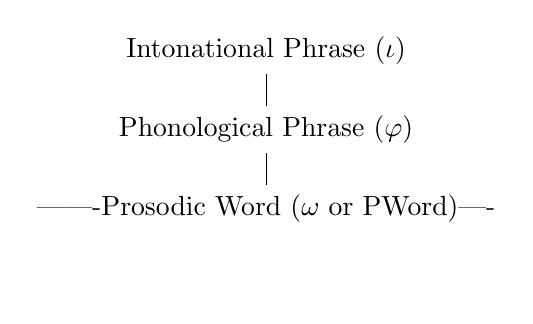
\begin{tikzpicture}[node distance = 1cm, auto]
				\node (6) [] {Intonational Phrase ($\iota$)}; 
				\node (5) [below of=6] {Phonological Phrase ($\varphi$)}; 
				\node (3) [below of=5] {-------Prosodic Word ($\omega$ or PWord)----}; 
				\node (2) [below of=3] { }; 
				
				\draw (6) -- (5);
				\draw (5) -- (3);
			\end{tikzpicture} 
			
			\ex ~\label{nlttPapertree hierarchy pstem redpaperhydbsbfsv}
			
			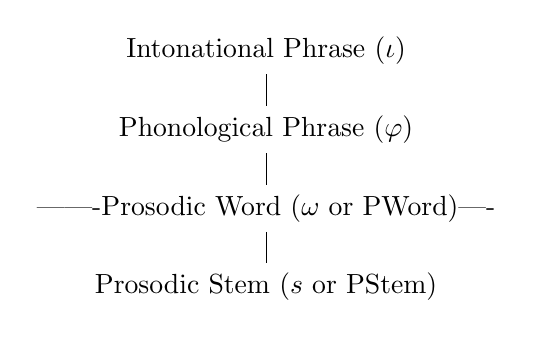
\begin{tikzpicture}[node distance = 1cm, auto]
				\node (6) [] {Intonational Phrase ($\iota$)}; 
				\node (5) [below of=6] {Phonological Phrase ($\varphi$)}; 
				\node (3) [below of=5] {-------Prosodic Word ($\omega$ or PWord)----}; 
				\node (2) [below of=3] {Prosodic Stem ($s$ or PStem)}; 
				
				\draw (6) -- (5);
				\draw (5) -- (3);
				\draw (3) -- (2);
			\end{tikzpicture}
		\end{xlist}
	\end{multicols}
	
\end{exe}

\begin{exe}
	\ex \label{nlttPapertree hierarchy table wesbdthewegashr}
	
	\begin{tabular}{ll}
		a. &b. \\
		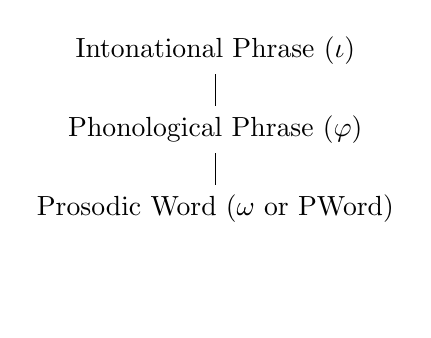
\begin{tikzpicture}[node distance = 1cm, auto]
			\node (6) [] {Intonational Phrase ($\iota$)}; 
			\node (5) [below of=6] {Phonological Phrase ($\varphi$)}; 
			\node (3) [below of=5] {Prosodic Word ($\omega$ or PWord)}; 
			\node (2) [below of=3] {\textcolor{white}{(}}; 
			
			\draw (6) -- (5);
			\draw (5) -- (3);
		\end{tikzpicture} 
		& 
		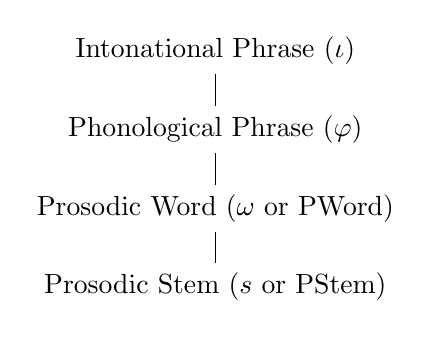
\begin{tikzpicture}[node distance = 1cm, auto]
			\node (6) [] {Intonational Phrase ($\iota$)}; 
			\node (5) [below of=6] {Phonological Phrase ($\varphi$)}; 
			\node (3) [below of=5] {Prosodic Word ($\omega$ or PWord)}; 
			\node (2) [below of=3] {Prosodic Stem ($s$ or PStem)}; 
			
			\draw (6) -- (5);
			\draw (5) -- (3);
			\draw (3) -- (2);
		\end{tikzpicture}
		
	\end{tabular}
	\begin{multicols}{2}
		
		\begin{xlist}
			\ex ~\label{nlttPapertree hierarchy traditional redpaperhydbsbfsv} 
			
			
			\ex ~\label{nlttPapertree hierarchy pstem redpaperhydbsbfsv}
			
		\end{xlist}
	\end{multicols}
	
\end{exe}


Just as syntactic phrases and morphological words are the sources of prosodic phrases and prosodic words, MStems are the source of PStems. The bulk of the evidence for the PStem comes from agglutinative languages and language families \citep{CzaykowskaHiggins-1997-MorphologicalPhonoConstituentSalish,Downing-2016-ProsodicLevelsChichewa}. The diagnostics used to detect PStems in other languages also show the PStem in Armenian. In Armenian, the overapplication of DHR straddles the boundary between the MStem and V-initial inflection. In other agglutinative languages, stem-level processes have been shown to be sensitive to the syllabification of MStems with V-initial suffixes or C-final prefixes. 
To illustrate, \citet{Aronoff-1988-HeadOperationsStrateRED} analyzes reduplication in KiHehe as targetting the morphological stem of the word (in italics). The reduplicant (underlined) is linearly found between inflectional prefixes and the stem (\ref{nlttPaperkihehe c redpapergbbdff}). The reduplicant generally copies only stem segments. But when the stem is V-initial, prefix-final consonants are copied because of syllabification (\ref{nlttPaperkihehe v redpapergbbdff}). 











\begin{exe}
	\ex 
	\begin{multicols}{2}
		\begin{xlist}
			\ex \makebox[3cm][l]{\textipa{ku-\textit{haata}}}`to ferment'\label{nlttPaperkihehe c redpapergbbdff}\\
			\makebox[3cm][l]{\textipa{ku-\underline{haata}$\sim${\textit{haata}}}}`to start fermenting'
			\ex \makebox[3cm][l]{\textipa{kw-\textit{iita}}}`to pour'\label{nlttPaperkihehe v redpapergbbdff}\\
			\makebox[3cm][l]{\textipa{\underline{kw-iita}$\sim${kw-\textit{iita}}}}`to start pouring'
		\end{xlist}
		
	\end{multicols}
\end{exe}

To explain prefix-copying in V-initial stems, \citet{Aronoff-1988-HeadOperationsStrateRED} analyzes reduplication as also targeting a prosodic head but does not formalize this concept. \citet{Downing-1998-ProsodicMisalignmentReduplication} reanalyzes KiHehe and formalizes the prosodic head as the PStem. It is mapped from the MStem, but it misaligns because of syllabification.

As a constituent, the PStem can be the target of reduplication, tonal processes, vowel harmony, minimality, and other sublexical processes \citep{Downing-1998-ProsodicMisalignmentOnsetlessNLLT,Downing-1999-ProsodicStem,Downing-1999-VerbalRed3BantuLanguages}. Further evidence for the PStem as a domain for phonological rules comes from cross-linguistic work on reduplication \citep{FitzpatrickCole-1994-ProsodicHierarchyReduplication,InkelasZoll2005-MorphoDouble,Shaw-2005-NonAdjacencyRed}, prefix-suffix asymmetries \citep{Hyman-2008-DirectionalAsymmetries}, minimality \citep{Downing-2005-MorphoCompelexityProsodicMinimality,Downing-2006-CanonicalForms}, strata \citep{Inkelas-1989-ProsodicLexicon,Inkelas-1993-DerivingCyclicity}, problems in bracket erasure \citep{Inkelas-2014-Interplay}, and bracketing paradoxes in compounds \citep{Han-1995-ProsodicStructureCompounds}. For a summary of the cross-linguistic evidence for the PStem, see \citet{Downing-2006-CanonicalForms,Downing-2016-ProsodicLevelsChichewa}, \citeauthor{DowningKadenge-2020-ReplacingPStemProsodicHierarchy} (to appear).

\subsubsection{The Prosodic Stem in Armenian}\label{nlttPapersection: reduction: destressed reduction EA: pstem: apply}
Applying the PStem to Armenian, I argue that MStems are mapped to non-recursive PStems while MWords are mapped to PWords. Before V-initial inflection, the PStem is misaligned from the MStem and expands. Before C-initial inflection, the PStem stays isomorphic with the MStem.


\begin{exe}
	\ex \textit{Different PStem structures in the two Armenian dialects.}\label{nlttPapertable: prosodic trees of EA WA} 
	
	\hspace*{-1cm}		\begin{tabular}{l|| l|l|l|l}
		\hline
		Type of structure&Base&Derivative&V-initial inflection&C-initial inflection\\\hline
		Morphology&
		\begin{tikzpicture}[scale = 0.8]
			
			\Tree [.MWord [.MStem \edge[roof];{{/\textipa{ɑmusin}/} -$\emptyset$} ] [.\textsc{nom} $\emptyset$ ] ] 
			
			
		\end{tikzpicture}
		&
		\begin{tikzpicture}[scale = 0.8]
			
			\Tree [.MWord [.MStem [.{MStem} \edge[roof];{{/\textipa{ɑmusin}/} -$\emptyset$} ] [.a /\textipa{-utjun}/ ] ] [ [.\textsc{nom} $\emptyset$ ] ] ] 
			
			
		\end{tikzpicture}
		&
		\begin{tikzpicture}[scale = 0.8]
			
			\Tree [.MWord [.MStem \edge[roof];{{/\textipa{ɑmusin}/} -$\emptyset$} ] [.{\ins} /\textipa{-ov}/ ] ] 
		\end{tikzpicture}
		&
		\begin{tikzpicture}[scale = 0.8]
			
			\Tree [.MWord [.MStem \edge[roof];{{/\textipa{ɑmusin}/} -$\emptyset$} ] [.{\pl} /\textipa{-ner}/ ] ] 
			
			
			
		\end{tikzpicture}
		\\\hline
		Prosody&
		\begin{tikzpicture}[scale = 0.75]
			\Tree [.PWord [.PStem \edge[roof];\textipa{ɑmus\'in} ] 					] 
			
			%	\Tree [.{Not Western Armenian} \edge[color=white];[.PWord [.PStem amusn-\'i ] ] 					]
			
		\end{tikzpicture}
		&
		\begin{tikzpicture}[scale = 0.75]
			\Tree [.PWord [.PStem \edge[roof];\textipa{ɑmusn-utj\'un} ] 					] 
			
			%	\Tree [.{Not Western Armenian} \edge[color=white];[.PWord [.PStem amusn-\'i ] ] 					]
			
		\end{tikzpicture}
		&
		\begin{tikzpicture}[scale = 0.75]
			
			\Tree [.PWord [.PStem \edge[roof];\textipa{ɑmus(i)n-\'ov} ] ] 				 
		\end{tikzpicture}
		&
		\begin{tikzpicture}[scale = 0.75]
			\Tree [.PWord [.PStem \edge[roof];\textipa{ɑmusin} ] [.$\sigma$ \textipa{-n\'er} ] 					] 
			
			%	\Tree [.{Not Western Armenian} \edge[color=white];[.PWord [.PStem amusn-\'i ] ] 					]
			
		\end{tikzpicture}
		\\\hline
		
		
	\end{tabular}
	
\end{exe} 



I argue that the PStem is indexed with its own cophonology. In EArm, the PStem triggers Stress Shift and Destressed High Vowel Reduction (DHR) but not Destressed Diphthong \textit{uj-}Reduction (DDR).\footnote{In order for the EArm PStem-level cophonology to trigger high vowel reduction but not diphthong reduction, we need the ranking: \textsc{*Reduce^2} $>>$ *\textit{\v{i},\v{u}} $>>$ {\textsc{ Id[f]} $>>$ \textsc{Max-V}} $>>$ *\textit{\v{uj}}. The faithfulness constraints \textsc{Id[f],Max-V} are outranked by *\textit{\v{i},{u}}. This triggers high vowel reduction. However, these faithfulness constraints outrank *\textit{\v{uj}}. This ranking blocks *\textit{\v{uj}} from triggering high diphthong reduction. The constraint \textsc{*Reduce^2} also dominates *\textit{\v{i},\v{u}}. This prevents \text{*\textit{\v{i},\v{u}}} from triggering diphthong reduction. \label{nlttPaperfootnote destressed diphtohng pstem}
} This is more than the stem-level cophonology, and less than the word-level cophonology. In WArm, the PStem cophonology is equivalent to the word-level stratum. It triggers stress shift but not reduction. 







\begin{exe}
	\ex \textit{Distribution of processes and domains across cophonologies}\\
	
	\begin{tabular}{l | llll}
		Morphological domain&Derivation&\multicolumn{2}{c}{V-initial Inflection}&Inflection\\
		Relevant constituent&MStems&\multicolumn{2}{c}{Misaligned PStems}&MWords\\
		Cophonology&Stem-level&\multicolumn{2}{c}{PStem-level}& Word-level\\
		% Domain&MStems&\mulExpanded PStem=MStem + V-Infl.&MWord\\
		\hline
		backslashbox[71mm]{Process}{Dialect} &Both&EArm&WArm&Both\\\cline{2-5}
		Destressed Diphthong \textit{uj} Reduction (DDR) &\ding{51} &\ding{55} &\ding{55} &\ding{55} \\
		Destressed High Vowel Reduction (DHR)&\ding{51} &\ding{51} &\ding{55} &\ding{55} \\
		Stress Shift &\ding{51} &\ding{51} &\ding{51} &\ding{51} \\
		
	\end{tabular}
\end{exe}


The stem-level and word-level strata are morphologically triggered by derivation and inflection. In contrast, the PStem-level cophonology is an intermediate cophonology: it applies after the stem-level and before the word-level when the right prosodic conditions are met. Specifically, it applies when V-initial inflection is added to an MStem and PStem misalignment: \textit{\textipa{//(a.mu.si.n)_s-ov// $\rightarrow$(a.mu.si.n-ov)_s}}. I stipulate that the PStem-cophonology \textit{only} occurs when we have PStem misalignment. I formalize the constraints needed (S\ref{nlttPapersection: reduction: destressed reduction EA: pstem: apply: constreaint}) to generate the PStem in uninflected (S\ref{nlttPapersection: reduction: destressed reduction EA: pstem: apply: der}) and inflected words (S\ref{nlttPapersection: reduction: destressed reduction EA: pstem: apply: infl}).

\subsubsubsection{Overview and constraint definitions}\label{nlttPapersection: reduction: destressed reduction EA: pstem: apply: constreaint} 

I use the following constraints adapted from \textsc{Match} theory \citep{Selkirk-2011-SyntaxPhonoInterface}. I have adapted them for mapping PStems \citep{Downing-1999-VerbalRed3BantuLanguages}, for mapping nested domains (\ref{nlttPaperconstraint: pstem wrapstem redpapertgdfsnd}; \citealt{Truckenbrodt-1999-RelationSyntaxPhonologyWRAP}), and for mapping non-isomorphic PStems (\ref{nlttPaperconstraint: pstem overmatch redpapertgdfsnd},\ref{nlttPaperconstraint: pstem undermatch redpapertgdfsnd}; \citealt{Guekguezian-2017-ProsodicRecursionCyclicityWord,Guekguezian-2017-TemplatesInteractionRecursionWordProsodic}). 



\begin{exe}
	\ex 
	\begin{xlist}
		\ex \textsc{MatchStem} $\sim$ \textsc{Match}: An MStem must correspond to a PStem\label{nlttPaperconstraint: pstem match redpapertgdfsnd}
		\ex \textsc{OverMatch} $\sim$ \textsc{Over}: A PStem does not contain a segment which isn't in its MStem (= overparse)\label{nlttPaperconstraint: pstem overmatch redpapertgdfsnd}
		\ex \textsc{UnderMatch} $\sim$ \textsc{Under}: A PStem does not lack a segment which isn't in its MStem (= underparse)\label{nlttPaperconstraint: pstem undermatch redpapertgdfsnd}
		\ex \textsc{AlignSyll} $\sim$ \textsc{Align}: A PStem must be aligned with syllable boundaries \label{nlttPaperconstraint: pstem alignsyll redpapertgdfsnd}
		\ex \textsc{NonRec}: PStems cannot be recursive\label{nlttPaperconstraint: pstem nonrec redpapertgdfsnd}
		\ex \textsc{WrapStem} or $\sim$ \textsc{Wrap}: An MStem must either a) correspond to a PStem, or b) be dominated by an MStem which corresponds to a PStem\label{nlttPaperconstraint: pstem wrapstem redpapertgdfsnd}
		
		
	\end{xlist}
\end{exe}

Contra \citet{Selkirk-2011-SyntaxPhonoInterface}, \citet{Elfner-2015-RecursionProsodicPhrasingIrish}, and \citet{Truckenbrodt-1999-RelationSyntaxPhonologyWRAP}, I define these constraints in terms of correspondence, not in terms of matching terminal nodes. I use the term `mapping' to mean the creation of PStems and of establishing a correspondence relationship between MStems and PStems \citep[cf. correspondence relations in ][]{MccarthyPrince-1995-Reduplication,itoMester-2019-matchSyntaxProsodyMaxDepProsodicEnclisisEnglish}. The constraint \textsc{MatchStem} requires that an MStem is mapped to a PStem, i.e., it is in correspondence with a PStem. The constraint does not require that a PStem contains all, only, or any of the segments of the MStem. The constraints \textsc{UnderMatch}, \textsc{OverMatch} handle what segments are contained in the PStem. \textsc{WrapStem} is a weaker version of \textsc{MatchStem} that allows an MStem's segments to be parsed into a higher MStem's PStem.%. A MStem is wrapped into a PStem by being in correspondence with the PStem, or by being dominated by a larger MStem which is in correspondence with the PStem. %If a candidate violates \textsc{WrapStem} then it also violates \textsc{MatchStem}; but a candidate can violate \textsc{MatchStem} without violating \textsc{WrapStem}. The constraint \textsc{MatchStem} will be shown to be inactive due to high-ranking \textsc{NonRec} and \textsc{WrapStem}. %ithat the MStem is in correspo It requires .% They are ranked differently in WArm and EArm, showing that the dialects vary in some but not all of their prosodic constraints The constraints \textsc{AlignSyll}, \textsc{NonRec}, and \textsc{WrapStem} are undominated and not violated on the surface.

\subsubsubsection{Mapping non-recursive PStems in roots and derivatives}\label{nlttPapersection: reduction: destressed reduction EA: pstem: apply: der}

In (\ref{nlttPaperderivation table: stratal prosody amusin amusnutjun}), I show the condensed cyclic derivation of the free-standing root \textit{\textipa{ɑmusi\'n}} and its derivative \textit{\textipa{ɑmusn-utj\'un}}. I use an explicit prosody step for syllabification and PStem mapping. Both uninflected MStems are parsed to a single non-recursive PStem. Without PStem misalignment, these words don't undergo the PStem-cophonology. MStems are marked with \{...\}\textsubscript{S} in the input, PStems with (...)\textsubscript{s} in the output. 

% \begin{exe}
	
	% \ex 
	% \begin{xlist}
		
		% \ex \makebox[3cm][l]{Base}\makebox[3cm][l]{\textipa{ɑmus\'in}}\makebox[3cm][l]{`husband'}\label{nlttPaperexample: warm earm reduce high list repeat: base} 
		% \ex \makebox[3cm][l]{Der. Suffix}\makebox[3cm][l]{\textipa{ɑmusn-utj\'un}}\makebox[3cm][l]{`marriage'}\label{nlttPaperexample: warm earm reduce high list repeat: der} 
		% %\ex \makebox[3cm][l]{Compound}\makebox[3cm][l]{\textipa{s\'er}}\makebox[3cm][l]{`love'}\label{nlttPaperexample: warm earm reduce high list repeat: compound}\\
		% %\makebox[3cm][l]{}\makebox[3cm][l]{\textipa{ɑmusn-a-s\'er}}\makebox[3cm][l]{`loving one's husband'} 
		% \ex \makebox[3cm][l]{V-initial Infl.}\makebox[3cm][l]{\textipa{ɑmusn-\'ov}}\makebox[4cm][l]{`husband-{\ins}'}EArm\label{nlttPaperexample: warm earm reduce high list repeat: V inf ea} 
		% \ex \makebox[3cm][l]{}\makebox[3cm][l]{\textipa{ɑmusin-\'ov}}\makebox[4cm][l]{`husband-{\ins}'}WArm\label{nlttPaperexample: warm earm reduce high list repeat: V inf wa} 
		% \ex \makebox[3cm][l]{C-initial Infl.}\makebox[3cm][l]{\textipa{ɑmusin-n\'er}}\makebox[4cm][l]{`husband-{\pl}'}EArm, WArm\label{nlttPaperexample: warm earm reduce high list repeat: C inf both}
		% \end{xlist}\label{nlttPaperexample: warm earm reduce high list repeat}
	
	
	% \end{exe}

















\begin{exe}
	\ex \textit{Stratal and prosodic derivation of the root} \textipa{ɑmusin} \textit{and its derivative} \textipa{ɑmusn-utjun} \label{nlttPaperderivation table: stratal prosody amusin amusnutjun}\\
	
	\begin{tabular}{||llll l|| ll||}
		\hline
		
		% &&&
		% \begin{tikzpicture}[scale = 0.8]
			
			% 		\Tree [.MW_{\textsc{nom}} [.MS_{\textit{n}} [.$\sqrt{}$ /\textipa{ɑmusin}/ ] [.n -$\emptyset$ ] ] [ [.\textsc{nom} -$\emptyset$ ] ] ]
			
			% 		\end{tikzpicture} 
		% &
		% \begin{tikzpicture}[scale = 0.8]
			
			% 		\Tree [.MW_{nom} [.MS_{\textit{n}} [. MS_{\textit{n}} [.$\sqrt{}$ /\textipa{ɑmusin}/ ] [.n -$\emptyset$ ] ] ] [ [ [.n /\textipa{-utjun}/ ] ] ] ]
			
			% 		\end{tikzpicture} 
		
		% \\
		Input & &&& \textipa{/amusin -$\emptyset$_{S} /} & &\textipa{/amusin -$\emptyset$_{S1} -utjun_{S2}/} \\\hline\hline
		\textit{Cycle 1}& \textsc{Morph}& &Spell-out & \textipa{/amusin -$\emptyset$_{S} /} &\textit{Cycle 2} & \textipa{(a.mu.s\'in)_{s1} - /-utjun_{S2}}/ \\
		& \textsc{Prosody} &&Syllabify & \textipa{ɑ.mu.s\'in} & & \textipa{(a.mu.si.n)_{s1}-u.tjun} \\ 
		& &&Map PStem & \textipa{(a.mu.s\'in)_{s}} &&
		\textipa{(a.mu.si.n-u.tjun)_{s2}} \\
		& \textsc{Phono}& \textit{SLevel} &Stress & \textipa{(a.mu.s\'in)_{s}}& &\textipa{(a.mu.s\v{i}.n-u.tj\'un)_{s2}} \\
		&&&DHR && &\textipa{(a.mus.n-utj\'un)_s} 
		\\
		% && DHR & & \\
		% \hline
		% \\
		
		
		% \\
		% \\
		% \\
		% \hline
		% Cycle 3&\textsc{Morph}& Spell-out &\textipa{(amus\'in)_s /-$\emptyset$_W/} &\textipa{(amusn-utj\'un)_s /-$\emptyset$_W/} \\
		% & \textsc{Prosody} & Map PWord & \textipa{((amus\'in)_s)_w}& \textipa{((amusn-utj\'un)_s)_w} \\
		% & \textsc{Phono} & \textit{WLevel} & & \\
		% & & Stress & \textipa{((amus\'in)_s)_w}& \textipa{((amusn-utj\'un)_s)_w} \\
		
		\hline\hline
		Output& &&&\textipa{ɑmus\'in} && \textipa{ɑmusn-utj\'un} \\
		\hline 
	\end{tabular}
	
\end{exe}























In both dialects, a free-standing root forms an MStem that is mapped to an isomorphic PStem: \textit{\textipa{(amusin)_{s}}} (\ref{nlttPaperot tableau: base amusin}d). This is mandated by the parsing constraints \textsc{MatchStem} and \textsc{WrapStem} which are violated by the unparsed candidate (\ref{nlttPaperot tableau: base amusin}a). Constraint \textsc{UnderMatch} blocks candidates where no MStem segments are parsed (\ref{nlttPaperot tableau: base amusin}b), or only some are (\ref{nlttPaperot tableau: base amusin}c). Losing candidates (b,c) satisfy \textsc{MatchStem} because the MStem is in correspondence with a PStem, regardless of what the PStem contains. 






\begin{exe}
	\ex ~\\
	
	\vspace{-1cm}\label{nlttPaperot tableau: base amusin}\renewcommand*\arraystretch{1.2}
	\scalebox{1}[1]{\begin{tabular}[t]{|rrl||c:c:c:c:c:c|} \hline
			\multicolumn{3}{|c||}{\textipa{\{amusin\}_{S}}} & \textsc{Align} & \textsc{NonRec} & \textsc{Wrap} & \textsc{Match} & \textsc{Under} & \textsc{Over} \\[0.5ex]
			% \multicolumn{3}{|c||}{}& \textsc{Syll} & \textsc{} & \textsc{Stem} & \textsc{Stem} & \textsc{Match} & \textsc{Match} \\[0.5ex]
			
			% \multicolumn{3}{|c||}{} & \textsc{Syll} & \textsc{} & \textsc{Stem} & \textsc{Stem} & \textsc{Match} & \textsc{Match} \\[0.5ex]
			\hline
			\hline a. & & \textipa{ɑmusin} & & & $\ast$ & $\ast$ & & \\
			\hline b. & & \textipa{()_{s}amusin} & & & & & $\ast\ast\ast\ast\ast\ast$ & \\
			\hline c. & & \textipa{(amu)_{s}sin} & & & & & $\ast\ast\ast$ & \\
			\hline d. & \ding{43} & \textipa{(amusin)_{s}} & & & & & & \\
			\hline \end{tabular}} \renewcommand*\arraystretch{1} 
	
\end{exe}







In derived words like \textit{\textipa{ɑmusn-utjun}}, the two MStems are mapped to a single PStem: \textit{\textipa{(a.mu.si.n-utjun)_{s2}}} (\ref{nlttPaperot tableau: der amsuinutjun}k). The different numerical subscripts \textsubscript{1,2} 
mark the correspondence of different stems. The inner MStem \textit{S1} does not correspond to a PStem (= violates \textsc{MatchStem}) but it is dominated by an MStem which does have a PStem (= satisfies \textsc{WrapStem}). The required ranking is that \textsc{AlignSyll, NonRec, WrapStem} outrank \textsc{MatchStem}. I remove stress marks to reduce clutter.












\begin{exe}
	\ex ~\\
	
	\vspace{-1cm} \label{nlttPaperot tableau: der amsuinutjun} \resizebox{1\textwidth}{!}{%
		\renewcommand*\arraystretch{1.2}
		\scalebox{1}[1]{\begin{tabular}[t]{|l|rrl||c:c:c|c:c:c|} \hline
				&\multicolumn{3}{|c||}{\textipa{\{\{amusin\}_{S1}-utjun\}_{S2}}} & \textsc{Align} & \textsc{NonRec} & \textsc{Wrap} & \textsc{Match} & \textsc{Under} & \textsc{Over} \\[0.5ex]
				% &\multicolumn{3}{|c||}{}& \textsc{Syll} & \textsc{} & \textsc{Stem} & \textsc{Stem} & \textsc{Match} & \textsc{Match} \\[0.5ex]
				\hline \hline 
				\textit{Recursive }& a. & & \textipa{((amusi.n-u)_{s1}tjun)_{s2}} & & $\ast$! & & \cellcolor{lightgray} & \cellcolor{lightgray} & \cellcolor{lightgray}$\ast$ \\\cline{5-10}
				\textit{Candidates}& b. & & \textipa{((amusi.n)_{s1}-utjun)_{s2}} & $\ast$! & $\ast$! & & \cellcolor{lightgray} & \cellcolor{lightgray} & \cellcolor{lightgray} \\ \cline{5-10}
				& c. & & \textipa{((amusi)_{s1}n-utjun)_{s2}} & & $\ast$! & & \cellcolor{lightgray} & \cellcolor{lightgray}$\ast$ & \cellcolor{lightgray} \\
				
				\hline
				\textit{Unwrapped}
				& d. & & \textipa{(amusin-u)_{s1}tjun} & & & $\ast$! & \cellcolor{lightgray}$\ast$ & \cellcolor{lightgray} & \cellcolor{lightgray}$\ast$ \\\cline{5-10}
				\textit{Candidates}
				&e. & & \textipa{(amusi.n)_{s1}utjun} & $\ast$! & & $\ast$! & \cellcolor{lightgray}$\ast$ & \cellcolor{lightgray} & \cellcolor{lightgray} \\\cline{5-10}
				&f. & & \textipa{(amusi.)_{s1}n-utjun} & & & $\ast$! & \cellcolor{lightgray}$\ast$ & \cellcolor{lightgray}$\ast$ & \cellcolor{lightgray} \\
				\hline 
				\textit{Underparsed}
				&g. & & \textipa{(amusin-u)_{s2}tjun} & & & & $\ast$ & $\ast$!$\ast \ast \ast$ & \\
				\cline{5-10}
				\textit{Candidates}&h. & & \textipa{(amusi.n)_{s2}utjun} & $\ast$! & & & \cellcolor{lightgray}$\ast$ & \cellcolor{lightgray}$\ast \ast \ast \ast \ast$ & \cellcolor{lightgray} \\ \cline{5-10}
				&i. & & \textipa{(amusi.)_{s2}n-utjun} & & & & $\ast$ & $\ast$!$\ast \ast \ast \ast \ast$ & \\
				\hline \textit{Overparsed C.}& j. & & \textipa{(amusin-utjun)_{s1}} & & & $\ast$! & \cellcolor{lightgray}$\ast$ & \cellcolor{lightgray} & \cellcolor{lightgray}$\ast \ast \ast \ast \ast$ \\
				\hline &k. & \ding{43} & \textipa{(amusin-utjun)_{s2}} & & & & $\ast$ & & \\
				\hline \end{tabular}} \renewcommand*\arraystretch{1}
	}
\end{exe}

The constraints \textsc{AlignSyll, NonRec, WrapStem} are inviolable. High-ranking \textsc{AlignSyll} blocks candidates (\ref{nlttPaperot tableau: der amsuinutjun}b,e,h) where the PStem is not aligned with syllable boundaries: \textit{\textipa{(amusi.n)_{s1}utjun}} (b). High-ranking \textsc{NonRec} blocks candidates with recursive structure (a,b,c). High-ranking \textsc{WrapStem} blocks candidates (d,e,f) where the larger MStem \textit{S2} is not mapped to any PStem: \textit{\textipa{(amusin)_{s1}-utjun}} (e). Candidates (g,h,i) violate \textsc{UnderMatch} because MStem \textit{S2} is mapped to a small PStem \textit{s2}: \textit{\textipa{(amusin)_{s2}-utjun}} (h). The last losing candidate has MStem \textit{S1} map to a large PStem \textit{s1}: \textit{\textipa{(amusin-ujtun)_{s1}}}. Even though all the segments of MStem \textit{S2} are parsed inside a PStem $s1$, the candidate violates \textsc{WrapStem} because the larger MStem \textit{S2} is not in correspondence with any PStem.\footnote{I omit one logically possible candidate: \textit{\textipa{(amusinu-utjun)_{s1,2}}}. This candidate has a single large PStem. This PStem is in correspondence with both MStems. It only violates \textsc{OverMatch} because the PStem has 5 segments \textit{-utjun} which aren't in MStem \textit{S1}. It does not violate \textsc{MatchStem} or \textsc{WrapStem} because the MStems do have a correspondent PStem; these correspondents just happen to be the same PStem. I assume this candidate is not generated because a PStem cannot have multiple correspondents. 
} 


\subsubsubsection{Mapping misaligned PStems in inflection}\label{nlttPapersection: reduction: destressed reduction EA: pstem: apply: infl}

Before inflection, the shape of the PStem varies depending on the shape of the inflectional suffix. Briefly, V-initial inflection triggers resyllabification and PStem expansion. I \textit{stipulate} that PStem misalignment triggers the PStem-cophonology. This cophonology includes DHR in EArm. I illustrate below for the different inflected items with V-initial inflection: \textit{\textipa{ɑmusn-\'ov}} (EArm), \textit{\textipa{ɑmusin-\'ov}} (WArm), and C-initial inflection: \textit{\textipa{ɑmusin-n\'er}}. %The variation in the shape of the PStem is due to a constraint \textsc{AlignSyll} that requires PStems to align with syllable boundaries. % Table (\ref{nlttPaperderivation table: strata prosody amusinov amusnov amusinner}) illustrates this. 

















\begin{exe}
	\ex \textit{Stratal and prosodic derivation of} \textipa{ɑmusn-ov} (EArm), \textipa{ɑmusin-ov} (WArm), \textit{and} \textipa{ɑmusin-ner} (both)\label{nlttPaperderivation table: strata prosody amusinov amusnov amusinner}\\
	
	\hspace*{-1.25cm}\resizebox{1.05\textwidth}{!}{%\hspace*{-1.2cm}
		\begin{tabular}{||lll l| lll||}
			\hline
			&&&&EArm & WArm & EArm \&WArm\\
			
			% &&&
			% \begin{tikzpicture}[scale = 0.8]
				
				% 		\Tree [.MW_{{\ins}} [.MS_{\textsc{n}} [.$\sqrt{}$ /\textipa{ɑmusin}/ ] [.\textit{n} -$\emptyset$ ] ] [ [.{\ins} \textipa{/-ov/} ] ] ] 
				
				% 		\end{tikzpicture} 
			% &
			% \begin{tikzpicture}[scale = 0.8]
				
				% 		\Tree [.MW_{{\ins}} [.MS_{\textsc{n}} [.$\sqrt{}$ /\textipa{ɑmusin}/ ] [.\textit{n} -$\emptyset$ ] ] [ [.{\ins} \textipa{/-ov/} ] ] ] 
				
				% 		\end{tikzpicture} 
			% &
			% \begin{tikzpicture}[scale = 0.8]
				
				% 		\Tree [.MW_{{\pl}} [.MS_{\textsc{n}} [.$\sqrt{}$ /\textipa{ɑmusin}/ ] [.\textit{n} -$\emptyset$ ] ] [ [.{\pl} \textipa{/-ner/} ] ] ] 
				
				% 		\end{tikzpicture} 
			
			% \\
			Input & && &\textipa{/amusin -$\emptyset$_S -ov_W/} & \textipa{/amusin -$\emptyset$_S -ov_W/} & \textipa{/amusin -$\emptyset$_S -ner_W/} \\\hline\hline
			Cycle 1 & & & & \textipa{(a.mu.s\'in)_s} & \textipa{(a.mu.s\'in)_s} & \textipa{(a.mu.s\'in)_s} \\
			\hline\hline
			Cycle 2 &\textsc{Morph}&& Spell-out & \textipa{(a.mu.s\'in)_s - /-ov_W}/ & \textipa{(a.mu.s\'in)_s - /-ov_W}/ & \textipa{(a.mu.s\'in)_s - /-ner_W}/ \\
			%Cycle 2a 
			& \textsc{Prosody} &&Syllabify &\textipa{(a.mu.s\'i.n)_s-ov}&\textipa{(a.mu.s\'i.n)_s-ov}&\textipa{(a.mu.s\'in)_s-ner} \\
			% Cycle 2b
			& && Readjust PStem &\textipa{(a.mu.s\'i.n-ov)_s}&\textipa{(a.mu.s\'i.n-ov)_s}& \\
			% & & Map PWord &\textipa{((a.mu.si.n-ov)_s)_w}&\textipa{((a.mu.sin-ov)_s)_w}&{\textipa{((amusin)_s-ner)_w}} \\\hline
			% Cycle 2c 
			& \textsc{Phono}& \textit{PStem-level} & Stress &\textipa{(a.mu.s\v{i}.n-\'ov)_s}&\textipa{(a.mu.s\v{i}.n-\'ov)_s}&\cellcolor{lightgray} \\
			&&& DHR (EArm) & \textipa{(a.mus.n-\'ov)_s}&\cellcolor{lightgray}&\cellcolor{lightgray} \\
			% \hline
			% Cycle 2d & \textsc{Phono}& \textit{PStem-level} (WArm) &\cellcolor{lightgray} &&\cellcolor{lightgray} \\
			% && Stress &\cellcolor{lightgray}&\textipa{((a.mu.s\v{i}.n-\'ov)_s)_w}& \cellcolor{lightgray}\\
			% \hline
			% Cycle 2d 
			& \textsc{Phono} & \textit{WLevel}& Stress&\textipa{(a.mu.sn-\'ov)_s}&\textipa{((a.mu.sin-\'ov)_s}&\textipa{(a.mu.sin)_s-n\'er)}\\\hline\hline
			Output&&&& \textipa{ɑmusn-\'ov}&\textipa{ɑmusin-\'ov}&\textipa{ɑmusin-n\'er} \\
			\hline 
		\end{tabular}
	}
\end{exe}




Given the base \textit{\textipa{(a.mu.sin)_s}}, inflection is spelled out and syllabified in Cycle 2. 
Before C-initial inflection, the PStem stays isomorphic with the MStem and with syllable boundaries. C-initial inflection is PStem-external: \textit{\textipa{(a.mu.sin)_s-ner}}. Before V-initial inflection, the PStem becomes misaligned from syllable boundaries: \textit{\textipa{*(a.mu.si.n)_s-ov}}. To repair this, the PStem is readjusted by incorporating the V-initial inflectional suffix: \textit{\textipa{(a.mu.si.n-ov)_s}}. The PStem cophonology is then triggered for the misaligned PStems. EArm's PStem triggers stress and DHR \textit{\textipa{ɑmusn-\'ov}}, WArm's PStem only triggers stress \textit{\textipa{ɑmusin-\'ov}}. The MWord is mapped to a PWord, and the word-level phonology applies.% reduction in. For the C-initial suffix \textit{\textipa{(amusin)_s-ner}}, the PStem is not misaligned so the PStem-level cophonology does not apply. The PStem-level cophonology only applies for V-initial inflection: \textit{\textipa{(amusin-ov)_s}}. High vowel reduction is in the PStem-level cophonology of EArm but not of WArm. In EArm in Cycle 2c, the PStem-level cophonology applies with DHR: \textit{\textipa{(amusn-ov})_s}. But in WArm in Cycle 2d, the PStem-level cophonology applies without DHR: \textit{\textipa{(amusin-\'ov)_s}}. The PStem-level cophonology in WArm is thus the same as the word-level cophonology. The word-level cycle then applies for all inflected words. These various changes in PStem shape are formalized in the appendix by ranking \textsc{AlignSyll} with various \textsc{Match} constraints. 








% In Table (\ref{nlttPapertable: prosodic trees of EA WA}), I summarize the morphological and prosodic structure for the different items in (\ref{nlttPaperexample: warm earm reduce high list repeat}). For ease of contrast, the non-terminal nodes are labelled as MWords, PWords, MStems, and PStems. I show covert inflection for the root and derivative.



I formalize the prosody step in Cycle 2 where the PStem is potentially readjusted before inflection. Before C-initial inflection in \textit{amusin-ner}, the PStem is isomorphic with the MStem and syllable boundaries because it violates no parsing constraints: \textit{\textipa{(a.mu.sin)_s-ner}} (\ref{nlttPaperot tableau: c initiai inf}). The losing candidates are harmonically bounded by the winner.



\begin{exe}
	\ex ~\\
	
	\vspace{-1cm}\label{nlttPaperot tableau: c initiai inf} \renewcommand*\arraystretch{1.2}
	\scalebox{1}[1]{\begin{tabular}[t]{|rrl||c:c:c|c:c:c|} \hline
			\multicolumn{3}{|c||}{\textipa{\{amusin\}_{S}-ner}} & \textsc{Align} & \textsc{NonRec} & \textsc{Wrap} & \textsc{Match} & \textsc{Under} & \textsc{Over} \\[0.5ex]
			% \multicolumn{3}{|c||}{}& \textsc{Syll} & \textsc{} & \textsc{Stem} & \textsc{Stem} & \textsc{Match} & \textsc{Match} \\[0.5ex]
			\hline \hline a. & \ding{43} & \textipa{(amusin)_{s}-ner} & & & & & & \\
			\hline b. & & \textipa{(amusin-ner)_{s}} & & & & & & $\ast\ast\ast$ \\
			\hline c. & & \textipa{ɑmusin-ner} & & & $\ast$! & \cellcolor{lightgray}$\ast$ & \cellcolor{lightgray} & \cellcolor{lightgray} \\
			\hline \end{tabular}} \renewcommand*\arraystretch{1} 
	
\end{exe}

% So far, there is no ranking among the constraints. But before V-initial inflection, mismatches are created and we see the need for constraint ranking: high-ranked \textsc{AlignSyll, WrapStem}. Crucially, the dialects will have different rankings of \textsc{UnderMatch} and \textsc{OverMatch} \citep[cf.][]{Anttila-2002-MorpholConditionedPhonoAlternation}. 

In both dialects, misalignment or non-isomorphism occurs in V-initial inflection due to syllabification (\ref{nlttPaperot tableau: v inf}). The losing faithful candidate \textit{\textipa{(a.mu.si.n)_s-ov}} violates the undominated constraint \textsc{AlignSyll}. To repair this, the PStem can be either contracted \textit{\textipa{(a.mu.si)_sn-ov}} (= violate \textsc{UnderMatch}) or expanded \textit{\textipa{(a.mu.si.n-ov)_s}} (= violate \textsc{OverMatch}). I argue it expands in both dialects. This means {\textsc{OverMatch}} outranks \textsc{UnderMatch}. Both constraints are dominated by \textsc{AlignSyll}. Regardless of misalignment, a PStem must be formed because \textsc{WrapStem} is undominated (cf. candidate d).

\begin{exe}
	% \ex
	% \begin{xlist}
		\ex ~\\
		
		\vspace{-1cm}\label{nlttPaperot tableau: v inf WA}\label{nlttPaperot tableau: v inf} \renewcommand*\arraystretch{1.2}
		\scalebox{1}[1]{\begin{tabular}[t]{|rrl||c:c|c|c|} \hline
				\multicolumn{3}{|c||}{\textipa{\{amusin\}_{S}-ov}} & \textsc{Wrap} &\textsc{Align} & \textsc{Under} & \textsc{Over} \\[0.5ex]
				\hline \hline a. & & \textipa{(amusi.n)_{s}-ov} && $\ast$! & \cellcolor{lightgray} & \cellcolor{lightgray} \\
				\hline b. & & \textipa{(amusi)_{s}n-ov} & & & $\ast$! & \cellcolor{lightgray} \\
				\hline c. & \ding{43} & \textipa{(amusin-ov)_{s}} & & & & \cellcolor{lightgray}$\ast\ast$ \\
				\hline d. & & \textipa{ɑmusin-ov} & $\ast!$ & & \cellcolor{lightgray} & \cellcolor{lightgray} \\
				\hline \end{tabular}} \renewcommand*\arraystretch{1} 
		
		
		
		
		% \ex \textit{Mapping PStems in }/\textipa{ɑmusin-ov}/ [\textipa{ɑmusn-ov]} \textit{with V-initial inflection in Eastern Armenian}\label{nlttPaperot tableau: v inf EA}
		
		% \renewcommand*\arraystretch{1.2}
		% \scalebox{1}[1]{\begin{tabular}[t]{|rrl||c:c|c|c|} \hline
				% \multicolumn{3}{|c||}{\textipa{{amusin}_S-ov}} & \textsc{Wrap} &\textsc{AlignSyll} & \textsc{OverMatch} & \textsc{UnderMatch} \\[0.5ex]
				% \hline \hline a. & & \textipa{(amusi.n)_s-ov} && $\ast$! & \cellcolor{lightgray} & \cellcolor{lightgray} \\
				% \hline b. &\ding{43} & \textipa{(amusi)_sn-ov} & & & & \cellcolor{lightgray}$\ast$ \\
				% \hline c. & & \textipa{(amusin-ov)_{s}} & & & $\ast!\ast$& \cellcolor{lightgray} \\
				% \hline d. & & \textipa{ɑmusin-ov} & $\ast!$ & & \cellcolor{lightgray} & \cellcolor{lightgray} \\
				% \hline \end{tabular}} \renewcommand*\arraystretch{1} 
		
		% \end{xlist}
	
\end{exe}





% In Table (\ref{nlttPapertable: prosodic trees of EA WA}), I summarize the morphological and prosodic structure for the different items in (\ref{nlttPaperexample: warm earm reduce high list repeat}). For ease of contrast, the non-terminal nodes are labelled as MWords, PWords, MStems, and PStems. I show covert inflection for the root and derivative.




\section{old:dissPre-inflectional DHR in  the Prosodic Stem}\label{disssection: reduction: destressed reduction EA: pstem}

In modern Armenian DHR, the relevant morphological constituent is the MStem and the relevant cophonology is the stem-level cophonology.   In this section,  I argue that the relevant prosodic constituent \textit{X} is the Prosodic Stem or PStem \citep{Downing-1999-ProsodicStem}. I first summarize the  cross-linguistic evidence for the PStem, and show how the EArm data match that of other languages which have PStems. 

\subsubsection{The role of Prosodic Stems}\label{disssection: reduction: destressed reduction EA: pstem: role}

The traditional prosodic hierarchy assumes only three levels of morphosyntactically derived constituents: the prosodic word, the prosodic phrase, and the intonational phrase (\ref{disstree hierarchy traditional redchapterhydbsbfsv}).  However, there is  cross-linguistic work on morphologically complex languages  which  argues for a more enriched hierarchy that includes at least one constituent below the PWord: the Prosodic Stem (\ref{disstree hierarchy pstem redchapterhydbsbfsv}).\footnote{The Prosodic Root (PRoot) has also been posited as a constituent mapped from morphological roots. The evidence for the PRoots, however, is less than for PStems. } 



\begin{exe}
	\ex 
	\begin{multicols}{2}
		
		\begin{xlist}
			\ex ~\label{disstree hierarchy traditional redchapterhydbsbfsv} 
			
			\begin{tikzpicture}[node distance = 1cm, auto]
				\node (6) [] {Intonational Phrase ($\iota$)}; 
				\node (5) [below of=6] {Phonological Phrase ($\varphi$)}; 
				\node (3) [below of=5] {-------Prosodic Word ($\omega$ or PWord)----}; 
				\node (2) [below of=3] { }; 
				
				\draw (6) -- (5);
				\draw (5) -- (3);
			\end{tikzpicture}  
			
			\ex ~\label{disstree hierarchy pstem redchapterhydbsbfsv}
			
			\begin{tikzpicture}[node distance = 1cm, auto]
				\node (6) [] {Intonational Phrase ($\iota$)}; 
				\node (5) [below of=6] {Phonological Phrase ($\varphi$)}; 
				\node (3) [below of=5] {-------Prosodic Word ($\omega$ or PWord)----}; 
				\node (2) [below of=3] {Prosodic Stem ($s$ or PStem)}; 
				
				\draw (6) -- (5);
				\draw (5) -- (3);
				\draw (3) -- (2);
			\end{tikzpicture}
		\end{xlist}
	\end{multicols}
	
\end{exe}



Just as syntactic phrases and morphological words are the sources of prosodic phrases and prosodic words, MStems are the source of   PStems.  The bulk of the evidence for the PStem comes from agglutinative languages and language families \citep{CzaykowskaHiggins-1997-MorphologicalPhonoConstituentSalish,Downing-2016-ProsodicLevelsChichewa}.  The diagnostics used to detect PStems in other languages  also show  the PStem in Armenian. In Armenian, the  overapplication of DHR straddles the boundary between the MStem and V-initial inflection. In other agglutinative languages, stem-level processes have been shown to be sensitive to the syllabification of MStems with V-initial suffixes or C-final prefixes. 
To illustrate,  \citet{Aronoff-1988-HeadOperationsStrateRED} analyzes   reduplication in KiHehe   as targetting the morphological stem of the word (in italics).  The reduplicant   (underlined) is linearly found between inflectional prefixes and the stem (\ref{disskihehe c redchaptergbbdff}).   The reduplicant generally copies only stem segments. But    when the stem is V-initial, prefix-final consonants are copied  because of syllabification (\ref{disskihehe v redchaptergbbdff}).  





\begin{exe}
	\ex 
	\begin{multicols}{2}
		\begin{xlist}
			\ex \makebox[3cm][l]{\textipa{ku-\textit{haata}}}`to ferment'\label{disskihehe c redchaptergbbdff}\\
			\makebox[3cm][l]{\textipa{ku-\underline{haata}$\sim${\textit{haata}}}}`to start fermenting'
			\ex \makebox[3cm][l]{\textipa{kw-\textit{iita}}}`to pour'\label{disskihehe v redchaptergbbdff}\\
			\makebox[3cm][l]{\textipa{\underline{kw-iita}$\sim${kw-\textit{iita}}}}`to start pouring'
		\end{xlist}
		
	\end{multicols}
\end{exe}

To explain  prefix-copying   in V-initial stems, \citet{Aronoff-1988-HeadOperationsStrateRED} analyzes reduplication as also targeting a prosodic head but does not formalize this concept.  \citet{Downing-1998-ProsodicMisalignmentReduplication} reanalyzes KiHehe   and formalizes the prosodic head as the PStem. It is mapped from the MStem, but it misaligns because of syllabification.

As a constituent, the PStem can be the target of reduplication, tonal processes, vowel harmony, minimality,  and other sublexical processes \citep{Downing-1998-ProsodicMisalignmentOnsetlessNLLT,Downing-1999-ProsodicStem,Downing-1999-VerbalRed3BantuLanguages}.   Further evidence for the PStem as a domain for phonological rules comes from cross-linguistic work on reduplication \citep{FitzpatrickCole-1994-ProsodicHierarchyReduplication,InkelasZoll2005-MorphoDouble,Shaw-2005-NonAdjacencyRed}, prefix-suffix asymmetries \citep{Hyman-2008-DirectionalAsymmetries}, minimality \citep{Downing-2005-MorphoCompelexityProsodicMinimality,Downing-2006-CanonicalForms}, strata \citep{Inkelas-1989-ProsodicLexicon,Inkelas-1993-DerivingCyclicity}, problems in bracket erasure \citep{Inkelas-2014-Interplay}, and   bracketing paradoxes in compounds \citep{Han-1995-ProsodicStructureCompounds}. For a summary of the cross-linguistic evidence for the PStem, see \citet{Downing-2006-CanonicalForms,Downing-2016-ProsodicLevelsChichewa},  \citeauthor{DowningKadenge-2020-ReplacingPStemProsodicHierarchy} (to appear).

\subsubsection{The Prosodic Stem in Armenian}\label{disssection: reduction: destressed reduction EA: pstem: apply}
Applying the PStem to Armenian, I argue that MStems are mapped to non-recursive PStems while MWords are mapped to PWords. Before V-initial inflection, the PStem is misaligned from the MStem and expands. Before C-initial inflection, the PStem stays isomorphic with the MStem.


\begin{exe}
	\ex  \textit{Different PStem structures   in the two Armenian dialects.}\label{disstable: prosodic trees of EA WA} 
	
	\hspace*{-1cm}		\begin{tabular}{l|| l|l|l|l}
		\hline
		Type of structure&Base&Derivative&V-initial inflection&C-initial inflection\\\hline
		Morphology&
		\begin{tikzpicture}[scale = 0.8]
			
			\Tree [.MWord [.MStem \edge[roof];{{/\textipa{ɑmusin}/}  -$\emptyset$} ]    [.\textsc{nom} $\emptyset$ ] ]  
			
			
		\end{tikzpicture}
		&
		\begin{tikzpicture}[scale = 0.8]
			
			\Tree [.MWord [.MStem [.{MStem} \edge[roof];{{/\textipa{ɑmusin}/}  -$\emptyset$} ]   [.a /\textipa{-utjun}/ ] ]   [ [.\textsc{nom} $\emptyset$ ] ] ]  
			
			
		\end{tikzpicture}
		&
		\begin{tikzpicture}[scale = 0.8]
			
			\Tree [.MWord [.MStem \edge[roof];{{/\textipa{ɑmusin}/}  -$\emptyset$} ]   [.\textsc{inst} /\textipa{-ov}/ ] ]  
		\end{tikzpicture}
		&
		\begin{tikzpicture}[scale = 0.8]
			
			\Tree [.MWord [.MStem \edge[roof];{{/\textipa{ɑmusin}/}  -$\emptyset$} ]   [.\textsc{pl} /\textipa{-ner}/ ] ]  
			
			
			
		\end{tikzpicture}
		\\\hline
		Prosody&
		\begin{tikzpicture}[scale = 0.75]
			\Tree [.PWord [.PStem \edge[roof];\textipa{ɑmus\'in} ] 					] 
			
			%	\Tree [.{Not Western Armenian} \edge[color=white];[.PWord [.PStem amusn-\'i ] ] 					]
			
		\end{tikzpicture}
		&
		\begin{tikzpicture}[scale = 0.75]
			\Tree [.PWord [.PStem \edge[roof];\textipa{ɑmusn-utj\'un} ] 					] 
			
			%	\Tree [.{Not Western Armenian} \edge[color=white];[.PWord [.PStem amusn-\'i ] ] 					]
			
		\end{tikzpicture}
		&
		\begin{tikzpicture}[scale = 0.75]
			
			\Tree [.PWord [.PStem \edge[roof];\textipa{ɑmus(i)n-\'ov} ] ] 				 
		\end{tikzpicture}
		&
		\begin{tikzpicture}[scale = 0.75]
			\Tree [.PWord [.PStem \edge[roof];\textipa{ɑmusin} ] [.$\sigma$ \textipa{-n\'er} ] 					] 
			
			%	\Tree [.{Not Western Armenian} \edge[color=white];[.PWord [.PStem amusn-\'i ] ] 					]
			
		\end{tikzpicture}
		\\\hline
		
		
	\end{tabular}
	
\end{exe} 



I argue that the PStem is indexed with its own cophonology. In EArm, the PStem triggers  Stress Shift and   Destressed High Vowel Reduction (DHR) but not Destressed Diphthong \textit{uj-}Reduction (DDR). This is more than the stem-level cophonology, and less than the word-level cophonology. In WArm, the PStem cophonology is equivalent to the word-level stratum. It triggers stress shift but not   reduction. 






\begin{exe}
	\ex \textit{Distribution of processes and domains across cophonologies}\\
	
	\begin{tabular}{l | llll}
		Morphological domain&Derivation&\multicolumn{2}{c}{V-initial Inflection}&Inflection\\
		Relevant constituent&MStems&\multicolumn{2}{c}{Misaligned PStems}&MWords\\
		Cophonology&Stem-level&\multicolumn{2}{c}{PStem-level}& Word-level\\
		% Domain&MStems&\mulExpanded PStem=MStem + V-Infl.&MWord\\
		\hline
		backslashbox[71mm]{Process}{Dialect}  &Both&EArm&WArm&Both\\\cline{2-5}
		Destressed Diphthong \textit{uj} Reduction (DDR) &\ding{51}    &\ding{55}  &\ding{55}  &\ding{55} \\
		Destressed High Vowel  Reduction (DHR)&\ding{51}    &\ding{51}  &\ding{55}  &\ding{55} \\
		Stress Shift &\ding{51}    &\ding{51}  &\ding{51}  &\ding{51} \\
		
	\end{tabular}
\end{exe}


The stem-level and word-level strata are morphologically triggered by derivation and inflection. In contrast, the PStem-level cophonology is an intermediate cophonology: it applies after the stem-level and before the word-level when the right prosodic conditions are met. Specifically, it applies when V-initial inflection is added to an MStem and causes the misalignment of the PStem: \textit{\textipa{(a.mu.sin)_s $\rightarrow$ //(a.mu.si.n)_s-ov// $\rightarrow$(a.mu.si.n-ov)_s}}. I stipulate that the PStem-cophonology \textit{only} occurs when we have PStem misalignment. 

Without inflection, an MStem is mapped to an isomorphic   PStem as a prosodic process.\footnote{In the table, the prosodic mapping of a PStem is    a separate step or rule in the serial derivation   \citep[cf.][]{Selkirk-1980-ProsodicDomainSanskrit,Nespor-Vogel-1986-ProsodicPhon,Selkirk-1986-DerivedDomains,Gunes-2015-TurkishDerivingProsody}. An alternative parallelist formalization is to adapt constraints from   \textsc{Match} theory and \textsc{Wrap} theory \citep{Selkirk-2011-SyntaxPhonoInterface,Truckenbrodt-1999-RelationSyntaxPhonologyWRAP,Guekguezian-2017-ProsodicRecursionCyclicityWord,Guekguezian-2017-TemplatesInteractionRecursionWordProsodic} for PStems. }  In (\ref{dissderivation table: stratal prosody amusin amusnutjun}), I show the condensed cyclic derivation of the free-standing root \textit{\textipa{ɑmusi\'n}}   and its derivative  \textit{\textipa{ɑmusn-utj\'un}}. Both are uninflected. 
% by using the data in (\ref{dissexample: warm earm reduce high list repeat}), repeated from (\ref{dissexample: warm earm reduce high list}) but omitting compounds.




%  \begin{exe}
	
	% \ex 
	% \begin{xlist}
		
		% \ex \makebox[3cm][l]{Base}\makebox[3cm][l]{\textipa{ɑmus\'in}}\makebox[3cm][l]{`husband'}\label{dissexample: warm earm reduce high list repeat: base} 
		% \ex \makebox[3cm][l]{Der. Suffix}\makebox[3cm][l]{\textipa{ɑmusn-utj\'un}}\makebox[3cm][l]{`marriage'}\label{dissexample: warm earm reduce high list repeat: der} 
		% %\ex \makebox[3cm][l]{Compound}\makebox[3cm][l]{\textipa{s\'er}}\makebox[3cm][l]{`love'}\label{dissexample: warm earm reduce high list repeat: compound}\\
		% %\makebox[3cm][l]{}\makebox[3cm][l]{\textipa{ɑmusn-a-s\'er}}\makebox[3cm][l]{`loving one's husband'} 
		% \ex \makebox[3cm][l]{V-initial Infl.}\makebox[3cm][l]{\textipa{ɑmusn-\'ov}}\makebox[4cm][l]{`husband-\textsc{inst}'}EArm\label{dissexample: warm earm reduce high list repeat: V inf ea} 
		% \ex \makebox[3cm][l]{}\makebox[3cm][l]{\textipa{ɑmusin-\'ov}}\makebox[4cm][l]{`husband-\textsc{inst}'}WArm\label{dissexample: warm earm reduce high list repeat: V inf wa} 
		% \ex \makebox[3cm][l]{C-initial Infl.}\makebox[3cm][l]{\textipa{ɑmusin-n\'er}}\makebox[4cm][l]{`husband-\textsc{pl}'}EArm, WArm\label{dissexample: warm earm reduce high list repeat: C inf both}
		% \end{xlist}\label{dissexample: warm earm reduce high list repeat}
	
	
	%  \end{exe}

















\begin{exe}
	\ex \textit{Stratal and prosodic derivation of the root} \textipa{ɑmusin}  \textit{and its derivative} \textipa{ɑmusn-utjun} \label{dissderivation table: stratal prosody amusin amusnutjun}\\
	
	\begin{tabular}{||llll  l|| ll||}
		\hline
		
		% &&&
		% \begin{tikzpicture}[scale = 0.8]
			
			% 		\Tree  [.MW_{\textsc{nom}} [.MS_{\textit{n}} [.$\sqrt{}$ /\textipa{ɑmusin}/ ]  [.n  -$\emptyset$ ] ]  [ [.\textsc{nom}  -$\emptyset$ ]  ] ]
			
			% 		\end{tikzpicture} 
		% &
		% \begin{tikzpicture}[scale = 0.8]
			
			% 		\Tree  [.MW_{nom} [.MS_{\textit{n}} [. MS_{\textit{n}} [.$\sqrt{}$ /\textipa{ɑmusin}/ ] [.n  -$\emptyset$ ] ]  ]  [ [ [.n  /\textipa{-utjun}/ ] ]  ]  ]
			
			% 		\end{tikzpicture} 
		
		% \\
		Input   & &&& \textipa{/amusin -$\emptyset$_S /} & &\textipa{/amusin -$\emptyset$_S -utjun_S/}  \\\hline\hline
		\textit{Cycle 1}& \textsc{Morph}& &Spell-out  &  \textipa{/amusin -$\emptyset$_S /} &\textit{Cycle 2} & \textipa{(a.mu.s\'in)_s - /-utjun_S}/  \\
		&  \textsc{Prosody} &&Syllabify &  \textipa{ɑ.mu.s\'in} &      &    \textipa{(a.mu.si.n)_{s1}-u.tjun}  \\ 
		&   &&Map PStem &  \textipa{(a.mu.s\'in)_{s}} &&
		\textipa{(a.mu.si.n-u.tjun)_{s2}}   \\
		& \textsc{Phono}& \textit{SLevel}  &Stress  &  \textipa{(a.mu.s\'in)_s}&  &\textipa{(a.mu.s\v{i}.n-u.tj\'un)_s} \\
		&&&DHR && &\textipa{(a.mus.n-utj\'un)_s}  
		\\
		%  && DHR  &  & \\
		% \hline
		% \\
		
		
		%  \\
		%  \\
		%  \\
		%  \hline
		%  Cycle 3&\textsc{Morph}& Spell-out   &\textipa{(amus\'in)_s /-$\emptyset$_W/}  &\textipa{(amusn-utj\'un)_s /-$\emptyset$_W/}  \\
		%   &  \textsc{Prosody} & Map PWord &  \textipa{((amus\'in)_s)_w}&   \textipa{((amusn-utj\'un)_s)_w}  \\
		%  & \textsc{Phono} & \textit{WLevel}    &  &   \\
		%   & & Stress  &  \textipa{((amus\'in)_s)_w}&   \textipa{((amusn-utj\'un)_s)_w}  \\
		
		\hline\hline
		Output& &&&\textipa{ɑmus\'in} && \textipa{ɑmusn-utj\'un}  \\
		\hline 
	\end{tabular}
	
\end{exe}



In  Cycle 1,  the base is formed. The input MStem is syllabified and mapped to a PStem: \textit{\textipa{(amusin)}_s}. The stem-level phonological process of stress assignment applies: \textit{\textipa{(amus\'in)}}. In Cycle 2, the derivative is formed. The larger MStem is syllabified and prosodified as a larger non-recursive PStem: \textit{\textipa{(amus\'in-utjun)_s}}. The stem-level phonology applies again with stress shift and destressed high vowel reduction:  \textit{\textipa{(amusn-utj\'un)_s}}. In Cycle 3,   the MWord maps to a PWord for both the base and derivative. The word-level cophonology vacuously applies. The PStem-level cophonology does not apply because there is no misaligned PStem.







Before inflection, the PStem-level cophonology can apply   depending on the shape of the  suffix and of the PStem. I illustrate below for the different inflected items with V-initial inflection: \textit{\textipa{ɑmusn-\'ov}} (EArm), \textit{\textipa{ɑmusin-\'ov}} (WArm), and C-initial inflection: \textit{\textipa{ɑmusin-n\'er}}.  %The variation in the shape of the PStem is due to a constraint \textsc{AlignSyll} that requires PStems to align with syllable boundaries.   % Table (\ref{dissderivation table: strata prosody amusinov amusnov amusinner}) illustrates this. 















\begin{exe}
	\ex \textit{Stratal and prosodic derivation of}      \textipa{ɑmusn-ov} (EArm), \textipa{ɑmusin-ov} (WArm), \textit{and} \textipa{ɑmusin-ner} (both)\label{dissderivation table: strata prosody amusinov amusnov amusinner}\\
	
	\hspace*{-1.25cm}\resizebox{1.05\textwidth}{!}{%\hspace*{-1.2cm}
		\begin{tabular}{||lll l| lll||}
			\hline
			&&&&EArm & WArm & EArm \&WArm\\
			
			% &&&
			% \begin{tikzpicture}[scale = 0.8]
				
				% 		\Tree  [.MW_{\textsc{inst}} [.MS_{\textsc{n}} [.$\sqrt{}$ /\textipa{ɑmusin}/ ]  [.\textit{n}  -$\emptyset$ ] ] [  [.\textsc{inst} \textipa{/-ov/} ]  ] ]  
				
				% 		\end{tikzpicture} 
			% &
			% \begin{tikzpicture}[scale = 0.8]
				
				% 		\Tree  [.MW_{\textsc{inst}} [.MS_{\textsc{n}} [.$\sqrt{}$ /\textipa{ɑmusin}/ ]  [.\textit{n}  -$\emptyset$ ] ] [  [.\textsc{inst} \textipa{/-ov/} ]  ] ]  
				
				% 		\end{tikzpicture} 
			% &
			% \begin{tikzpicture}[scale = 0.8]
				
				% 		\Tree  [.MW_{\textsc{pl}} [.MS_{\textsc{n}} [.$\sqrt{}$ /\textipa{ɑmusin}/ ]  [.\textit{n}  -$\emptyset$ ] ] [  [.\textsc{pl} \textipa{/-ner/} ]  ] ]  
				
				% 		\end{tikzpicture} 
			
			% \\
			Input &  && &\textipa{/amusin -$\emptyset$_S -ov_W/} & \textipa{/amusin -$\emptyset$_S  -ov_W/}  & \textipa{/amusin -$\emptyset$_S  -ner_W/}  \\\hline\hline
			Cycle 1 & &  & & \textipa{(a.mu.s\'in)_s}  &  \textipa{(a.mu.s\'in)_s}  &  \textipa{(a.mu.s\'in)_s} \\
			\hline\hline
			Cycle 2 &\textsc{Morph}&& Spell-out  &  \textipa{(a.mu.s\'in)_s - /-ov_W}/ & \textipa{(a.mu.s\'in)_s - /-ov_W}/ & \textipa{(a.mu.s\'in)_s - /-ner_W}/  \\
			%Cycle 2a 
			&  \textsc{Prosody} &&Syllabify &\textipa{(a.mu.s\'i.n)_s-ov}&\textipa{(a.mu.s\'i.n)_s-ov}&\textipa{(a.mu.s\'in)_s-ner}  \\
			% Cycle 2b
			& &&  Readjust PStem  &\textipa{(a.mu.s\'i.n-ov)_s}&\textipa{(a.mu.s\'i.n-ov)_s}&  \\
			%   & &  Map PWord   &\textipa{((a.mu.si.n-ov)_s)_w}&\textipa{((a.mu.sin-ov)_s)_w}&{\textipa{((amusin)_s-ner)_w}}  \\\hline
			% Cycle 2c 
			& \textsc{Phono}& \textit{PStem-level}  & Stress  &\textipa{(a.mu.s\v{i}.n-\'ov)_s}&\textipa{(a.mu.s\v{i}.n-\'ov)_s}&\cellcolor{lightgray} \\
			&&& DHR (EArm) &  \textipa{(a.mus.n-\'ov)_s}&\cellcolor{lightgray}&\cellcolor{lightgray}  \\
			%  \hline
			% Cycle 2d & \textsc{Phono}& \textit{PStem-level} (WArm)  &\cellcolor{lightgray} &&\cellcolor{lightgray} \\
			%  && Stress  &\cellcolor{lightgray}&\textipa{((a.mu.s\v{i}.n-\'ov)_s)_w}& \cellcolor{lightgray}\\
			%  \hline
			% Cycle 2d 
			&  \textsc{Phono} & \textit{WLevel}&  Stress&\textipa{(a.mu.sn-\'ov)_s}&\textipa{((a.mu.sin-\'ov)_s}&\textipa{(a.mu.sin)_s-n\'er)}\\\hline\hline
			Output&&&& \textipa{ɑmusn-\'ov}&\textipa{ɑmusin-\'ov}&\textipa{ɑmusin-n\'er} \\
			\hline 
		\end{tabular}
	}
\end{exe}




Given the    base \textit{\textipa{(a.mu.sin)_s}}, inflection is spelled out and syllabified in Cycle 2. Before C-initial inflection, the PStem stays isomorphic with the MStem and with syllable boundaries. C-initial inflection is PStem-external: \textit{\textipa{(a.mu.sin)_s-ner}}. Before V-initial inflection, the PStem becomes misaligned from syllable boundaries: \textit{\textipa{*(a.mu.si.n)_s-ov}}. To repair this,  the PStem is readjusted   by   incorporating the V-initial inflectional suffix:  \textit{\textipa{(a.mu.si.n-ov)_s}}.\footnote{In an earlier analysis \citep{dolatian-2017-CLS2PublicationArm,dolatian-2019-PLCArmenianCycles}, I argued that the PStem contracted in WArm: \textit{\textipa{(a.mu.si.)_sn-ov}}. The PStem-level cophonology was the same in both dialects. I argued that PStem expansion would trigger DHR while PStem contraction would not. I have changed the analysis to make the illustration easier. Both analyses work, but the current analysis fits better with the variation data.} The PStem cophonology is then triggered    for the misaligned PStems. EArm's PStem triggers stress and DHR \textit{\textipa{ɑmusn-\'ov}}, WArm's PStem only triggers stress \textit{\textipa{ɑmusin-\'ov}}. The MWord is mapped to a PWord, and the word-level phonology applies.% reduction in. For the C-initial suffix \textit{\textipa{(amusin)_s-ner}}, the PStem is not misaligned so the PStem-level cophonology does not apply. The PStem-level cophonology only applies for V-initial inflection: \textit{\textipa{(amusin-ov)_s}}. High vowel reduction is in the PStem-level cophonology of EArm but not of WArm. In EArm in Cycle 2c, the PStem-level cophonology applies with DHR:  \textit{\textipa{(amusn-ov})_s}.  But in WArm in Cycle 2d, the PStem-level cophonology applies without DHR: \textit{\textipa{(amusin-\'ov)_s}}. The PStem-level cophonology in WArm is thus the same as the word-level cophonology.    The word-level cycle then applies for all inflected words.  These various changes in PStem shape are formalized in the appendix by ranking \textsc{AlignSyll} with various \textsc{Match} constraints. 








% In  Table (\ref{disstable: prosodic trees of EA WA}), I summarize the morphological and prosodic structure for the different items in (\ref{dissexample: warm earm reduce high list repeat}). For ease of contrast, the non-terminal nodes are labelled as MWords, PWords, MStems, and PStems. I show covert inflection for the root and derivative.

\subsection{High vowel reduction and prosodic misalignment }\label{disssection: reduction: destressed reduction EA: pword and feet}

The previous section showed that   pre-inflectional   DHR depends on  whether the inflectional suffix is V- vs.\ C-initial. This points to syllabification as a possible factor.   Specifically, pre-inflectional  DHR correlates with the misalignment of the MStem (= the base) and syllables. Before C-initial inflection, the MStem ends in a syllable: \textit{\textipa{ɑmusin.-n\'er}}. Before V-initial inflection, the MStem boundary and syllable boundary are not aligned: \textit{\textipa{ɑmusi.n-\'ov}$\rightarrow$amusn-\'ov}. 


Cross-linguistically, morphological constituents often get misaligned from syllable boundaries. When misaligned, phonological processes  can apply differently. This suggests that the relevant phonological process references a prosodic constituent that is mapped from the morphology. For example,  English level-1 suffixes are mostly V-initial and  trigger the stem-level rule of stress shift, while level-2 suffixes are mostly  C-initial and do not trigger stress shift (\ref{dissexample: english pword misalignment}). Dutch has similar misalignment patterns \citep{Oostendorp-2004-CrossingMorphemeBoundariesDutch}.






\begin{exe}
	
	
	\ex \makebox[3cm][l]{\textit{(m\'edicine)_w}}\makebox[4cm][l]{\textit{(s\'ynonym)_w}}\makebox[3cm][l]{\textit{(\'ɑccurate)_w}}\makebox[4cm][l]{\textit{(dev\'elop)_w}}\label{dissexample: english pword misalignment} \\
	\makebox[3cm][l]{\textit{(med\'icin-al)_w}}\makebox[4cm][l]{\textit{(syn\'onym-ous)_w}}\makebox[3cm][l]{\textit{(\'ɑccurate)_w-ness}}\textit{(dev\'elop)_w-ment}
	
	
\end{exe} 


\cite{Raffelsiefen-1999-PhonoConstraintEnglishWords,Raffelsiefen-2005-ParadigmvsBoundary} analyzed stress shift as caused by the misalignment of the prosodic word (PWord). V-initial suffixes  are outside the MWord but they incorporate into the PWord. By incorporating, these suffixes cause the PWord to expand and trigger the stem-level phonology. In other words, English stress-shift applies whenever the PWord gets larger than the MWord. 

I argue for a similar analysis for Armenian. The MStem maps to some prosodic constituent \textit{X}. Before V-initial inflection,  \textit{X} gets misaligned from syllable boundaries and must expand. In WArm, the expansion of \textit{X} has no effect. But in EArm, the expansion of \textit{X} triggers pre-inflectional DHR. The problem is defining what \textit{X} is. In this section, I show that two common prosodic constituents (feet and PWords) are unlikely to be involved in DHR. The evidence points to a distinct prosodic constituent which mediates between feet and PWords: the Prosodic Stem (PStem).



\subsubsection{Feet as the domain of pre-inflectional DHR}\label{disssection: reduction: destressed reduction EA: pword and feet: feet}

%In this section, I show that the relevant constituent \textit{X} cannot be the foot.
One hypothetical solution is to have \textit{X} be a foot: the stem-level cophonology creates  feet which later trigger  pre-inflectional DHR \citep[cf.][]{Anttila-2006-VariationOpacityFinnish}. But  it is unclear how feet would  trigger pre-inflectional DHR. Both V-initial and C-initial suffixes take final stress and would form iambic feet. I sketch out a failed analysis below for the two inflected items \textit{\textipa{ɑmusn-\'ov, amusin-n\'er}}.




\begin{exe}
	\ex \textit{A failed hypothetical derivation using feet}\\
	
	\hspace*{-1.5cm}
	\begin{tabular}{||lll|ll|}
		\hline\hline
		Input&&&\textipa{/amusin -$\emptyset$_S -ov_W/}&\textipa{/amusin -$\emptyset$_S -ner_W/}\\
		\hline\hline
		\textit{Cycle 1  } && 
		&\textipa{ɑ.(mu.s\'in)}&\textipa{ɑ.(mu.s\'in)}  \\
		\hline
		\textit{Cycle 2}& 
		\textsc{Morph}&Spell-out suffix&\textipa{ɑ.(mu.s\'in) /-ov/}&\textipa{ɑ.(mu.s\'in) /-ner/}\\
		&\textsc{Prosody}&Syllabify  suffix&\textipa{ɑ.(mu.s\'i.n)-ov}&\textipa{ɑ.(mu.s\'in)-ner}\\
		
		&&Align foot with syllables&\textipa{ɑ.mu.(s\'i.n-ov)}& \\
		& \textsc{Phono}&Stress \& {Shift feet}&\textipa{ɑ.mu.(s\v{i}.n-\'ov)}&\textipa{ɑ.mu.(s\v{i}n-n\'er)}\\
		&&DHR in 1\textsuperscript{st} syllable of foot&\textipa{ɑ.(mus.n-\'ov)}&*\textipa{ɑ.mu.(s@n-n\'er)}\\
		
		\hline\hline
		\textit{Predicted Output}&&\textipa{ɑmusn-\'ov}&&*\textipa{ɑmus@n-n\'er}\\
		\textit{Correct Output}&&&\textipa{ɑmusn-\'ov}&\textipa{ɑmusin-n\'er}\\
		\hline\hline
		
	\end{tabular}
\end{exe}

At the end of the stem-level cycle, the base forms a final foot: \textit{\textipa{ɑ(mu.s\'in)}}. Upon syllabification with V-initial inflection, the   foot is misaligned from syllable boundaries: \textit{\textipa{ɑ.(mu.s\'i.n)-ov}}. This triggers shifting the foot to the suffix: \textit{\textipa{ɑmu(s\'in-ov)}}. Before C-initial inflection, no misalignment occurs and thus no shift (at first): \textit{\textipa{ɑ(mu.s\'in)-ner}}. 
So far the derivation shows a prosodic difference between V-initial vs.\ C-initial inflection: \textit{\textipa{ɑmu(s\'in-ov), a(mu.s\'in)-ner}}. At this stage, we could argue that DHR targets the first syllable of feet. But this analysis falls apart once we actually apply stress shift in the word-level:    \textit{\textipa{ɑmu.(s\v{i}n-n\'er)}}. Now, both V-initial and C-initial inflection have the same foot structure:   \textit{\textipa{ɑmu(s\v{i}n-\'ov), amu.(s\v{i}n-n\'er)}}.  If DHR is formulated to apply in the first syllable of feet, then we incorrectly predict reduction in both inflected words: \textit{\textipa{ɑmusin-\'ov, *amus@n-ner}}. Without additional machinery, pre-inflectional DHR cannot be formulated in terms of feet.\footnote{One workaround is to argue that DHR applies if the destressed syllable is 1) the weak part of an iambic foot, and 2) was aligned with the MStem in the input, but 3) is no longer aligned with the MStem in the output. This works; however it is then unclear what role is played by the feet. Conditions (2,3) are the descriptive generalizations and do trigger DHR; the use of feet (1) is superfluous.} Furthermore, as explained in S\ref{disssection: reduction: stress overview}, there is no independent evidence for iambic feet in Armenian.% evidence for iambic feet in  %Feet are irrelevant. 




\subsubsection{Recursive PWords and masking different domains}\label{disssection: reduction: destressed reduction EA: pword and feet: pword}

Instead of feet, we could argue that \textit{X} is a PWord. But this is problematic. All inflectional suffixes are incorporated into the PWord and   obligatorily trigger  the word-level process of  stress shift (\ref{dissexample: final stress earm pword}). Thus, the domain of final stress (inflection = the PWord) is larger than  the   domain  of DHR (V-initial inflection = X). 




% \begin{exe}
	% \ex 
	% \begin{multicols}{2}
		
		%  \begin{xlist}
			% \ex \makebox[2.5cm][l]{\textipa{tʰ\'uxtʰ}}\makebox[2.5cm][l]{\textipa{(tʰ\'uxtʰ)_w}}`paper'\\
			% \makebox[2.5cm][l]{\textipa{tʰ\'@xtʰ-\'ov}}\makebox[2.5cm][l]{\textipa{(tʰ@xtʰ-\'ov)_w}}`paper-\textsc{inst}'\\ 
			% \makebox[2.5cm][l]{\textipa{tʰ\'@xtʰ-\'er}}\makebox[2.5cm][l]{\textipa{(tʰ@xtʰ-\'er)_w}}`paper-\textsc{pl}'\\ 
			% \makebox[2.5cm][l]{\textipa{tʰ\'@xtʰ-er-\'ov}}\makebox[2.5cm][l]{\textipa{(tʰ@xtʰ-er-\'ov)_w}}`paper-\textsc{pl-inst}'
			% %\\\makebox[2.5cm][l]{\textipa{tʰ\'@xtʰ-er-\'ov} e}\makebox[2.5cm][l]{\textipa{(tʰ@xtʰ-er-\'ov)_w e}}`is paper-\textsc{pl-inst}'
			
			
			% \ex \makebox[2.6cm][l]{\textipa{ɑmus\'in}}\makebox[2.6cm][l]{\textipa{(amus\'in)_w}}`husband'\\
			% \makebox[2.6cm][l]{\textipa{ɑmusn-\'ov}}\makebox[2.6cm][l]{\textipa{(amusn-\'ov)_w}}`husband-\textsc{inst}'\\ 
			% \makebox[2.6cm][l]{\textipa{ɑmusin-n\'er}}\makebox[2.6cm][l]{\textipa{(amusin-n\'er)_w}}`husband-\textsc{pl}'\\ 
			% \makebox[2.6cm][l]{\textipa{ɑmusin-ner-\'ov}}\makebox[2.6cm][l]{\textipa{(amus-n-ner-\'ov)_w}}`husband-\textsc{pl-inst}'
			% %\\\makebox[2.6cm][l]{\textipa{ɑmusin-ner-\'ov}}\makebox[2.6cm][l]{\textipa{(amus-n-ner-\'ov)_w} e}`is husband-\textsc{pl-inst}'
			
			% \end{xlist}
		
		% \end{multicols}
	
	
	% \end{exe}





\begin{exe}
	\ex 
	
	\begin{xlist}
		
		\ex \makebox[2.6cm][l]{Base}\makebox[2.6cm][l]{\textipa{ɑmus\'in}}\makebox[2.8cm][l]{\textipa{(amus\'in)_w}}\makebox[3cm][l]{`husband'}\makebox[2cm][l]{\textit{Stress shift?}}\textit{Reduce?}
		\ex \makebox[2.6cm][l]{V-initial Infl.}\makebox[2.6cm][l]{\textipa{ɑmusn-\'ov}}\makebox[2.8cm][l]{\textipa{(amusn-\'ov)_w}}\makebox[3cm][l]{`husband-\textsc{inst}'}\makebox[2cm][l]{\textit{\ding{51}}}\textit{\ding{51}}
		\ex \makebox[2.6cm][l]{C-initial Infl.}\makebox[2.6cm][l]{\textipa{ɑmusin-n\'er}}\makebox[2.8cm][l]{\textipa{(amusin-n\'er)_w}}\makebox[3cm][l]{`husband-\textsc{pl}'}\makebox[2cm][l]{\textit{\ding{51}}}\textit{\ding{55}}
		\ex \makebox[2.6cm][l]{Stacked Infl.}\makebox[2.6cm][l]{\textipa{ɑmusin-ner-\'ov}}\makebox[2.8cm][l]{\textipa{(amusin-ner-\'ov)_w}}\makebox[3cm][l]{`husband-\textsc{inst-pl}'}\makebox[2cm][l]{\textit{\ding{51}}}\textit{\ding{55}}
		
		
	\end{xlist}\label{dissexample: final stress earm pword}
	
	
\end{exe}

This problem can't be fixed by pushing   stress-assignment to  a higher domain, e.g., a recursive   PWord' \citep{Peperkamp-1997-ProsodicWord,Selkirk-1996-ProsodicFunctionWords,ItoMester-2009-ExtendedProsodicWord,KabakRevithiadou-2009-InterfaceProsodicWordRecursionUgh} or the Clitic/Composite Group CG \citep{Vogel-2009-StatusCliticGroup,Vogel-2016-LifeAfterSLH}.  Enclitics are outside the stress domain and syllabify with word-final consonants (\ref{dissexample: earm clitic pword recursion}).   Clitics thus follow  a PWord boundary and belong to the PWord' or CG.  




\begin{exe}
	\ex \textit{Cliticization on...}\label{dissexample: earm clitic pword recursion}
	
	\begin{xlist}
		
		\ex \makebox[2.6cm][l]{Base}\makebox[3cm][l]{\textipa{ɑmus\'in} e}\makebox[3.5cm][l]{\textipa{(amus\'i)_w}n=e}`husband is'
		\ex \makebox[2.6cm][l]{V-initial Infl.}\makebox[3cm][l]{\textipa{ɑmusn-\'ov e}}\makebox[3.5cm][l]{\textipa{(amusn-\'o)_wv=e}}`husband-\textsc{inst} is' 
		\ex \makebox[2.6cm][l]{C-initial Infl.}\makebox[3cm][l]{\textipa{ɑmusin-n\'er} e}\makebox[3.5cm][l]{\textipa{(amusin-n\'e)_wr=e}}`husband-\textsc{pl} is' 
		\ex \makebox[2.6cm][l]{Stacked Infl.}\makebox[3cm][l]{\textipa{ɑmusin-ner-\'ov} e }\makebox[3.5cm][l]{\textipa{(amusin-ner-\'o)_wv=e}}`husband-\textsc{inst-pl} is' 
		
		
	\end{xlist}
	
	
\end{exe}


Disregarding clitics, one could argue that the relevant constituent is a minimal vs. maximal PWord (Berm\'udez-Otero, p.c.).  I illustrate below. In the word-level stratum, the base first forms a single PWord; this is before the syllabification of     V-initial or C-initial inflection: \textit{\textipa{(amusin)_w /-ov,-ner/}}. When V-initial inflection is syllabified, the MStem's PWord is misaligned from its syllable boundaries: \textit{\textipa{(a.mu.si.n)_w-ov}}. This triggers PWord expansion: \textit{\textipa{(amusin-ov)_w}}. Before C-initial inflection, there is no misalignment and the MWord is mapped to a recursive PWord: \textit{\textipa{((amusin)_w-ner)_w}}.





\begin{exe}
	\ex \textit{Hypothetical derivation using recursive PWords}
	
	\hspace*{-1cm}
	\begin{tabular}{||lll|ll|}
		\hline\hline
		Input&&&\textipa{/amusin -$\emptyset$_S -ov_W/}&\textipa{/amusin -$\emptyset$_S -ner_W/}\\
		\hline\hline
		\textit{Cycle 1  }&  & &\textipa{(a.mu.s\'in)_w}&\textipa{(a.mu.s\'in)_w}  \\
		\hline
		\textit{Cycle 2}& 
		\textsc{Morph}&Spell-out suffix&\textipa{(a.mu.s\'in)_w /-ov/}&\textipa{(a.mu.s\'in)_w /-ner/}\\
		&\textsc{Prosody}&Syllabify  suffix&\textipa{(a.mu.s\'i.n)_w-ov}&\textipa{(a.mu.s\'in)_w-ner}\\
		&&Align PWord with syllables&\textipa{(a.mu.s\'i.n-ov)_w}&\textipa{((a.mu.s\'in)_w-ner)}\\
		&&Map MWord to PWord&&\textipa{((a.mu.s\'in)_w-ner)_w}\\
		& \textsc{Phono}&Stress&\textipa{(a.mu.s\v{i}n.-\'ov)_w}&\textipa{((a.mu.s\v{i}n)_w-n\'er)_w}\\
		&&DHR&\textipa{(a.mus.n-\'ov)_w}&\textit{blocked}
		\\
		&&*\textit{blocked in  PWord-final $\sigma$}&&\\
		\hline\hline
		\textit{Output}&&\textipa{ɑmusn-\'ov}&\textipa{ɑmusin-n\'er}&\\\hline\hline
	\end{tabular}
\end{exe}

Moving on to the cophonologies, stress shift applies: \textit{\textipa{(amus\v{i}n-\'ov)_w}}, \textit{\textipa{((amus\v{i}n)_w-n\'er)_w}}. This analysis would argue that DHR is a word-level process and it apples inside PWords: \textit{\textipa{(amusn-\'ov)_w}}. A faithfulness constraint protects destressed high vowels in PWord-final syllables: \textit{\textipa{((amusin)_w-ner)_w}}.\footnote{This is essentially the same analysis in  \citet{Macak-2016-StudiesClassicalModernArmenianPhono}. The difference is that he doesn't use any strata and he uses weakly bracketed feet \citep{Hyde-2002-RestrictiveStressWeakBracketing}, e.g., \textit{\textipa{ɑ\textsubscript{(}mu\textsuperscript{(}sin\textsubscript{)}-n\'er\textsuperscript{)}}}, \textit{\textipa{*a\textsubscript{(}mu\textsuperscript{(}si\textsubscript{)}n-\'ov\textsuperscript{)}}}.} 

The problem with this analysis is that it argues that DHR is word-level in EArm. But there is evidence against this.  DHR does not apply in  regularized inflection (\ref{dissexample word level dhr irreg ygerfrtbsv}), inflected adjectives (\ref{dissexample word level dhr adj ygerfrtbsv}), or loanwords (\ref{dissexample word level dhr loan ygerfrtbsv}).   PWords are a common target for post-lexical rules which  tend to be   exceptionless and blind to the  diacritics  of individual lexemes. But, DHR  does not apply to every PWord. Furthermore,  post-cyclic lexical word-level rules  tend  to be exceptionless \citep{Pesetsky-1979-RussianMorphoLexicalTheory}. The   data show  that DHR has not generalized into a post-cyclic word-level process.     This   is further discussed in S\ref{disssection: reduction: variation: inf ea} in the context of DHR variation.  



\begin{exe}
	\ex 
	\begin{multicols}{3}
		\begin{xlist}
			\ex \makebox[2cm][l]{\textipa{mɑn\'uk}}`child'\label{dissexample word level dhr irreg ygerfrtbsv}\\
			\makebox[2cm][l]{\textipa{mank-ɑk\'ɑn}}`childish'\\
			\makebox[2cm][l]{\textipa{mank-\'ɑn}}\text{`child-\textsc{gen} (irreg.)'}\\
			\makebox[2cm][l]{\textipa{manuk-\'i}}`\text{child-\textsc{gen} (reg.)}'
			
			\ex \makebox[2cm][l]{\textipa{l\'ur\t{dZ}}}`serious'\label{dissexample word level dhr adj ygerfrtbsv}\\
			\makebox[2cm][l]{\textipa{l@r\t{dZ}-ɑn\'ɑl}}\text{`to get serious'}\\
			\makebox[2cm][l]{\textipa{lur\t{dZ}-\'i}}`serious-\textsc{gen}' \\
			
			
			\ex \makebox[2cm][l]{\textipa{f\'ilm}}`film'\label{dissexample word level dhr loan ygerfrtbsv}\\
			\makebox[2cm][l]{\textipa{film-ɑj\'in}}`cinematic'\\
			\makebox[2cm][l]{\textipa{film-\'er}}`film-\textsc{pl}' 
		\end{xlist}
		
	\end{multicols}
	
\end{exe}


Setting aside the  empirical problems above, using recursion is also conceptually problematic with unclear motivation.  
There is no explicit consensus on the behavior of recursive prosodic constituents. There is debate over whether recursive constituents can trigger categorically different processes vs.\ gradiently different processes \citep{Ladd-1986-IntonationalPhrasingRecursiveProsodic,ItoMester-2009-ExtendedProsodicWord,ItoMester-2012-RecursiveProsodicPhrasingJapanese,ItoMester-2013-ProsodicSubcategoriesJapanese,Wagner-2010-ProsodyRecursionCoordinate,FrotaVigario-2013-ProsodyMattersReview,Elfner-2015-RecursionProsodicPhrasingIrish}, whether they can block or trigger  lexical processes \citep{Szpyra-1989-PhonoMorphoInterface,Booij-1996-CliticizationProsodicIntegrationDutch,Peperkamp-1997-ProsodicWord,Raffelsiefen-2005-ParadigmvsBoundary,KabakRevithiadou-2009-InterfaceProsodicWordRecursionUgh,Bennett-2018-RecursiveProsodicWordMayan}, whether they are restricted to the post-lexical phonology of clitics \citep{Inkelas-1989-ProsodicLexicon,Booij-1996-CliticizationProsodicIntegrationDutch,Selkirk-1996-ProsodicFunctionWords,Zec-2005-ProsodicDifferenceFunctionWords,Tyler-2019-SimplifyingWordEnglishFunctionalCategories}, and whether they act as diacritics for  behaviorally different constituents \citep{Vogel-2009-StatusCliticGroup,Vogel-2012-Recursion,Vogel-2016-LifeAfterSLH,Vigario-2010-ProsodicWordGroupWordvsPhraseRecursionIndependentDomain,Guzzo-2018-ProsodicCompositePortugese,Miller-2018-PhonologySyntaxInterfacePolysynthesisKiowaSaulteauxOjibwe,Miller-2020-NavigatingPhonologySyntaxInterfaceTriPMapping}. 


To summarize,   there is no positive evidence that the relevant prosodic constituent \textit{X} should be the PWord. Treating \textit{X} as a recursive PWord masks the fact that DHR is a lexical process, not a gradient word-level process.  Pre-inflectional DHR instead references a prosodic constituent which is bigger than a foot yet smaller than a PWord, and bigger than an MStem yet smaller than the MWord. %The prosodic constituent triggers the overapplication of a stem-level process, not a word-level process. 






\section{Phonological life cycle}
\paragraph{old:nlltDomain narrowing from Classical to modern Armenian}\label{nlttPapersection: reduction: history of reduction in classical}

%This section acts as a segue to understanding how Eastern Armenian minimally differs from Western Armenian (WArm). 
The previous sections established the stratal and prosodic systems for the two modern Armenian dialects, mostly based on vowel reduction. One question is why the two dialects differ in the domain of DHR. In this section, I explain this difference by analyzing the history of reduction in Classical Armenian (CArm), the earliest attested variety of Armenian ($\sim$ 5\textsuperscript{th} century AD). I show how various destressed reduction processes underwent domain narrowing from the word-level in CArm to the stem-level in WArm or fossilization (S\ref{nlttPapersection: reduction: history of reduction in classical: CA is word level}). The analysis highlights the role of the phonological life-cycle as the origin of modern Armenian's strata. I speculate on what morphological factors encouraged domain narrowing from Classical to Modern Armenian (S\ref{nlttPapersection: reduction: history of reduction in classical: change}). I argue that these factors led to the emergence of the PStem cophonology (S\ref{nlttPapersection: reduction: history of reduction in classical: discussion}).% I apply the historical analysis to understand why diachronic analysis %In S\ref{nlttPapersection: reduction: history of reduction in classical: CA is word level}, I show that Destressed High Vowel and Diphthong \textit{uj-}Reduction were word-level processes in CArm. They narrowed in scope on their way to WArm. A contributing factor was that inflection changed from being fusional in CArm to agglutinative to WArm.
%In S\ref{nlttPapersection: reduction: history of reduction in classical: residuals of reduction in modern}, I note that CArm had other destressed reduction processes. But these became obsolete during the change from CArm to WArm. 
%LOST I then speculate on how destressed reduction probably arose in CArm in the first place via reanalysis (S\ref{nlttPapersection: reduction: history of reduction in classical: diachronic origin}).









\subsection{Morphological change and confounds in syllabification}\label{nlttPapersection: reduction: history of reduction in classical: change}

In this section, I argue that contributing factors to the domain narrowing are the significant changes in Armenian inflection. I later use these changes to explain how DHR diverged between EArm and WArm, and how they created the PStem.% created the PStem-level cophonology.


Nominal inflection in Classical Armenian was largely syncretic and fusional with the same suffix encoding number and case (\citeauthor{Adjarian-1909-ClassificationArmenianDialect} \citeyear[5]{Adjarian-1909-ClassificationArmenianDialect}, \citeauthor{HalleVaux-1998-IndoEuroNominalInflLatinArm} \citeyear[15]{HalleVaux-1998-IndoEuroNominalInflLatinArm}; \citealt{Donabedian-2000-ArmenianChangeClassicalModernTypology}; \citealt{Caha-2013-CaseNanosyntax}; \citeauthor{SayeedVaux-2017-EvolutionArmenian} \citeyear[1154]{SayeedVaux-2017-EvolutionArmenian}). But in modern Armenian, nominal inflection became agglutinative and less syncretic, with separate morphemes for number and case. The partial paradigms in (\ref{nlttPapertable: paradigm infl of CArm WArm}) illustrate this for regular inflection.\footnote{ For simplicity, I omit the locative because it hasn't survived into Western Armenian, but it has survived into Eastern Armenian (S\ref{nlttPapersection: reduction: destressed reduction EA: different reduction}). The segment \textit{-o-} can be segmented as a nominal theme vowel \citep{HalleVaux-1998-IndoEuroNominalInflLatinArm}; these theme vowels have not survived into modern Armenian nominal inflection as separate morphs. } %Remnants of fusional inflection survive in irregular declension classes (S\ref{nlttPapersection: reduction: destressed high reduction WA: inflection overapply}). 



\begin{exe}
	\ex \textit{Regular nominal inflection in Classical and Modern Western Armenian for the word `mouth'} \label{nlttPapertable: paradigm infl of CArm WArm}\\
	
	\hspace*{-1cm}\begin{tabular}{||l |l| llllll||}\hline\hline
		& & \textsc{Nom}& \textsc{Acc}& \textsc{Dat}& \textsc{Gen}& \textsc{Abl}& {\ins} \\\hline
		CArm & Singular & \textipa{beran} & \textipa{beran} & \textipa{beran-oj} & \textipa{beran-oj} & \textipa{beran-oj} & \textipa{beran-ow} \\
		& Plural & \textipa{beran-k} & \textipa{beran-s} & \textipa{beran-ot͡sʰ} & \textipa{beran-ot͡sʰ} & \textipa{beran-ot͡sʰ} & \textipa{beran-ow-k} \\
		WArm & Singular & \textipa{peran} & \textipa{peran} & \textipa{peran-i} & \textipa{peran-i} & \textipa{peran-e} & \textipa{peran-ov} \\
		& Plural & \textipa{peran-ner} & \textipa{peran-ner} & \textipa{peran-ner-u} & \textipa{peran-ner-u} & \textipa{peran-ner-e} & \textipa{peran-ner-ov} \\ \hline
		\hline \end{tabular}
	
	
\end{exe}

By becoming agglutinative, nominal inflection became more \textit{morphologically} distinguishable from derivation. This would make it easier to treat inflection as also \textit{phonologically} distinguishable from derivation. An additional change is the introduction of the stressable C-initial inflectional suffix \textit{-ner}. Unlike the modern dialects, CArm nominal inflection \textit{lacked} a stressable C-initial suffix which contains vowels.\footnote{On the surface, aorist formation in CArm verbal conjugation creates C-initial suffixes: \textit{sir-e-\textbf{t͡s}ʰ-i} `I loved'. But see \citet[217]{Hammalian-1984-PhonoOldArmenian} and \citet[205]{Macak-2016-StudiesClassicalModernArmenianPhono} on how this is actually derived from an underlying V-initial suffix /\textit{\textipa{-it͡sʰ}}/. Similar V-initial analyses are also extended to other apparent C-initial suffixes in the subjunctive \citep{Hammalian-1984-PhonoOldArmenian}. Besides, verbal inflection is morphologically stem-based in Armenian.} It only had unstressable lone-consonant suffixes: \textit{-k, -s}. In the next section, I argue that the creation of this new contrast between C-initial and V-initial inflection in modern Armenian plays a role in the development of DHR in Eastern Armenian. % (S\ref{nlttPapersection: reduction: destressed reduction EA}).

% In (\ref{nlttPapertable: domains across 2 carm warm}), I summarize the differences between Classical and Western Armenian in the domain of their prosodic processes. CArm did not distinguish between the stem- and word-level so I give it only one cophonology. WArm developed a new stem-level cophonology. Destressed High Vowel and Diphthong \textit{uj-}Reduction had narrowed from the word-level to the stem-level. Two other reduction processes, \textit{ja}- and \textit{\={e}}-reduction, narrowed from the word-level to being fossilized. 


% \begin{exe}
	% \ex \textit{Domain of prosodic processes across Classical and modern Western Armenian}\label{nlttPapertable: domains across 2 carm warm}\\
	
	% \hspace*{-1cm}
	% \begin{tabular}{|ll | lll | l|}
		% \hline\hline
		% Lect &Process &\multicolumn{3}{c|}{Morphological Domain} &Cophonology and status\\
		% & &Derivation & \multicolumn{2}{c|}{Inflection} & \\
		% & & & V-initial & C-initial & \\\hline
		
		% CArm & Stress Shift&\ding{51}&\ding{51} & & word-level\\
		% & High Vowel Reduction (DHR) &\ding{51}&\ding{51} && word-level\\
		% & Diphthong \textit{uj-}Reduction (DDR) &\ding{51}&\ding{51}& & word-level\\
		% & Diphthong \textit{ja-}Reduction &\ding{51}&\ding{51} && word-level\\
		% & \textit{\={e}-}Reduction &\ding{51}&\ding{51} && word-level\\\hline
		
		
		% WArm & Stress Shift&\ding{51}&\ding{51} & \ding{51} & stem-level and word-level\\
		% & High Vowel Reduction (DHR)&\ding{51}&\ding{55} &\ding{55} & stem-level \\
		% & Diphthong \textit{uj-}Reduction (DDR) &\ding{51}&\ding{55} & \ding{55} & stem-level \\
		% & Diphthong \textit{ja-}Reduction &$\sim$&\ding{55} & \ding{55} & fossilized\\
		% & \textit{\={e}-}Reduction &$\sim$&\ding{55} &\ding{55} & fossilized\\\hline
		
		
		
		
		
		
		% \end{tabular}
	
	% \end{exe}

%Note that in nominal inflection, Modern Armenian introduced a C-initial inflection suffix which \textit{could} trigger stress shift: the plural allomorph \textit{-ner} (S\ref{nlttPapersection: reduction: destressed high reduction WA: inflection overapply}).

% As mentioned in S\ref{nlttPapersection: reduction: history of reduction in classical: CA is word level}, CArm lacked stressable C-initial inflection unlike modern Armenian. Modern Armenian thus created a prosodic contrast between V-initial and C-initial inflection. In the next section, I show that the creation of this contrast causes Eastern Armenian (EArm) to display almost the same domain narrowing as WArm except for DHR: DHR overapplies in V-initial but not C-initial inflection. % Thus, the domain narrowing of DHR is incomplete in EArm due to syllabification and prosodic misalignment.










\subsection{Incomplete narrowing and the Prosodic Stem }\label{nlttPapersection: reduction: history of reduction in classical: discussion}
This section synthesizes the data from this paper in order to explain the microvariation of the two dialects as the consequence of morphological, prosodic, and historical factors. Three prosodic processes were studied: Stress Shift, Destressed High Vowel Reduction (DHR), and Destressed Diphthong \textit{uj}-Reduction (DDR). As shown in (\ref{nlttPapertable: domains across 3 carm warm earm}), these processes have different morphological domains in the three Armenian lects: Classical (CArm), modern Western (WArm), and modern Eastern (EArm).\footnote{ The sources listed in S\ref{nlttPapersection: reduction: history of reduction in classical} do not {explicitly} state that clitics do not trigger stress shift or reduction in CArm. I assume they do not because I have found no mention of it. } These different morphological domains correspond to different cophonologies. The narrowing of reduction processes from CArm to the modern dialects is predicted from the life-cycle of phonological processes \citep{Ramsammy-2015-LifeCyclephonoDialectalTypology}.




%I show that Armenian requires a fusion of lexical/stratal and prosodic phonology.% I briefly discuss an alternative cyclic model, e.g., phase-based phonology, and argue that it ultimately needs to adopt similar stratal or prosodic structure (S\ref{nlttPapersection: reduction: history of reduction in classical: discussion: phase}). %LOST I then explain that the role of strata mediates the controversy over the productivity of destressed reduction in modern Armenian (S\ref{nlttPapersection: reduction: history of reduction in classical: discussion: productivity}).
% \subsection{Domains in Armenian and Prosodic Lexical Phonology}\label{nlttPapersection: reduction: history of reduction in classical: discussion: domains prosodic lexical phonology}

%I set aside destressed \textit{ja-} and \textit{\={e}-}reduction (S\ref{nlttPapersection: reduction: history of reduction in classical: residuals of reduction in modern}). They were stem- and word-level in CArm but are now fossilized in WArm and EArm. I set aside hiatus rules for the modern dialects which still obey strata (S\ref{nlttPapersection: reduction: strata elsewhere in WA: stem edge and hiatus}) and misalignment (S\ref{nlttPapersection: reduction: pstem elsewhere: vowel hiatus EA}).




\begin{exe}
	\ex \textit{Domain of prosodic processes across Classical, Western, and Eastern Armenian}\label{nlttPapertable: domains across 3 carm warm earm}
	
	\hspace*{-1.3cm}
	\begin{tabular}{|ll | llll | l|}
		\hline\hline
		Process &Lect &\multicolumn{4}{c|}{Morphological Domain} &Cophonology \\
		& &Derivation & V-initial Infl. & C-initial Infl. & Clitics& \\\hline
		Stress & CArm & \ding{51}&\ding{51}&&\ding{55} & word-level\\
		& EArm & \ding{51}&\ding{51}&\ding{51}&\ding{55}& stem-, PStem-, word-level\\
		& WArm & \ding{51}&\ding{51}&\ding{51}&\ding{55}& stem-, PStem-, word-level\\\hline
		\textit{i,u} Reduction & CArm & \ding{51}&\ding{51}&&\ding{55}& word-level\\
		& EArm & \ding{51}&\ding{51}&\ding{55}&\ding{55}& stem-, PStem-level\\
		& WArm & \ding{51}&\ding{55}&\ding{55}&\ding{55}& stem-level\\\hline
		\textit{uj} Reduction & CArm & \ding{51}&\ding{51}&&\ding{55}& word-level\\
		& EArm & \ding{51}&\ding{55}&\ding{55}&\ding{55}&stem-level\\
		& WArm & \ding{51}&\ding{55}&\ding{55}&\ding{55}&stem-level\\
		\hline\hline
		
		
	\end{tabular}
	
\end{exe}


Classical Armenian did not show any word-internal stratification. I assume it only has one cophonology: a cyclic word-level cophonology. This cophonology has to be cyclic because of destressed reduction. Final stress has been constant in the three lects: it applies in every cophonology at every cycle. Reduction was word-level in CArm but it has narrowed in scope in the modern dialects. For most lexemes in WArm, both DHR and DDR have completely narrowed from the word-level to the stem-level. But in EArm, narrowing is partial. DDR has completely narrowed to the stem-level, but DHR occupies an intermediate zone: it applies in derivation, V-initial but not C-initial inflection. I modeled this zone as a separate cophonology: the PStem-level. This cophonology is triggered by prosodic misalignment of the Prosodic Stem. 

The question now is why DHR did not completely narrow down to the stem-level. The answer is the interaction of diachronic change and prosody. However, my answer is speculative at best because of limitations on the data between CArm and the modern dialects. 

Domain narrowing from CArm to the modern dialects was confounded with syllabification. Classical Armenian nominal inflection \textit{lacked} a stressable C-initial suffix which contains a vowel, while modern Armenian developed one: the plural \textit{-ner}.\footnote{This suffix appeared sometime during medieval or Middle Armenian \citep{Karst-1901-MiddleArmenain}. Future work will examine the stratal phonology of Middle Armenian.} I argue that this confound caused the emergence of the Prosodic Stem, i.e., the prosodic constituent which is mapped from misaligned (resyllabified) MStems before V-initial inflection. The PStem exists in both dialects as the site of appendixes like \textit{k} (S\ref{nlttPapersection: pstem elsewhere}).

In terms of domain narrowing and morphology, CArm only had V-initial inflection. When EArm learners developed a C-initial suffix, they reanalyzed DHR as applying only in V-initial inflection, not C-initial inflection. By reanalyzing DHR in terms of prosody (V-initiality), they narrowed DHR down to the PStem-level. In contrast in WArm, the PStem was still created; but, the above confound was ignored. Speakers generalized based on morphology (derivation vs. inflection) and DHR completely narrowed from word-level inflection to the stem-level. I have no theory as to why the two dialects chose different routes (prosody vs. morphology); my analysis only provides the existence of these two routes. 
%They narrowed DHR from the word-level to the PStem-level. In contrast, WArm learners ignored this confound and narrowed DHR down to the stem-level. 

%In all three lects, DHR is cyclic and can apply potentiaully unbounded number of times. 
%In Classical Armenian, DHR applied through derivation and inflection. But in modern Western Armenian, DHR has narrowed in scope and is sensitive to lexical strata. It applies in derivation but not inflection. Eastern Armenian also shows this stratal sensitivity. But in EArm, syllabification and prosodic misalignment creates a grey-zone for the domain of DHR. It can apply in V-initial inflection but not C-initial under various lexeme-level conditions.


% Prosody can also explain how some but not all stem-level rules can paradoxically be triggered by some but not all word-level morphology.





\paragraph{old:diss:change:story odmains causes}
\subsection{Morphological change   and confounds in syllabification}\label{disssection: reduction: history of reduction in classical: change}

In this section, I argue  that   contributing factors to the domain narrowing    are the significant changes in Armenian inflection. I later use these  changes  to explain  how DHR diverged between EArm and WArm, and how they created the PStem.% created the PStem-level cophonology.


Nominal inflection in Classical Armenian was largely syncretic and fusional with the same suffix encoding  number and case (\citeauthor{Adjarian-1909-ClassificationArmenianDialect} \citeyear[5]{Adjarian-1909-ClassificationArmenianDialect}, \citeauthor{HalleVaux-1998-IndoEuroNominalInflLatinArm} \citeyear[15]{HalleVaux-1998-IndoEuroNominalInflLatinArm}; \citealt{Donabedian-2000-ArmenianChangeClassicalModernTypology}; \citealt{Caha-2013-CaseNanosyntax};  \citeauthor{SayeedVaux-2017-EvolutionArmenian} \citeyear[1154]{SayeedVaux-2017-EvolutionArmenian}). But in modern  Western  Armenian, nominal inflection   became  agglutinative and less syncretic, with separate morphemes for number and case.  The partial paradigms in (\ref{disstable: paradigm infl of CArm WArm}) illustrate this  for regular inflection.\footnote{ For simplicity, I omit the locative because it hasn't survived into Western Armenian, but it has survived into Eastern Armenian (S\ref{disssection: reduction: destressed reduction EA: similar morphophono}). The segment \textit{-o-} can be segmented as a nominal theme vowel \citep{HalleVaux-1998-IndoEuroNominalInflLatinArm};   these theme vowels have not survived  into modern Armenian nominal inflection as separate morphs.} %Remnants of fusional inflection survive in irregular declension classes (S\ref{disssection: reduction: destressed high reduction WA: inflection overapply}). 




\begin{exe}
	\ex \textit{Regular nominal inflection in Classical and Modern Western Armenian for the word `mouth'} \label{disstable: paradigm infl of CArm WArm}\\
	
	\hspace*{-1cm}\begin{tabular}{||l |l| llllll||}\hline\hline
		&  &  \textsc{Nom}&  \textsc{Acc}&  \textsc{Dat}&  \textsc{Gen}&  \textsc{Abl}&  \textsc{Inst} \\\hline
		CArm &  Singular &  \textipa{beran} & \textipa{beran} & \textipa{beran-oj} & \textipa{beran-oj} & \textipa{beran-oj} & \textipa{beran-ow}  \\
		&  Plural &  \textipa{beran-k} & \textipa{beran-s} & \textipa{beran-o\t{ts}ʰ} & \textipa{beran-o\t{ts}ʰ} & \textipa{beran-o\t{ts}ʰ} & \textipa{beran-ow-k}  \\
		WArm &  Singular &  \textipa{peran} & \textipa{peran} & \textipa{peran-i} & \textipa{peran-i} & \textipa{peran-e} & \textipa{peran-ov}  \\
		&  Plural &  \textipa{peran-ner} & \textipa{peran-ner} & \textipa{peran-ner-u} & \textipa{peran-ner-u} & \textipa{peran-ner-e} & \textipa{peran-ner-ov}  \\ \hline
		\hline \end{tabular}
	
	
\end{exe}

By becoming agglutinative, nominal inflection became more \textit{morphologically} distinguishable from derivation. This would make it easier to treat inflection as also \textit{phonologically} distinguishable from derivation. An additional change is the introduction of the stressable C-initial inflectional suffix \textit{-ner}. Unlike the modern dialects, CArm nominal inflection  \textit{lacked} a stressable C-initial  suffix which contains vowels.\footnote{On the surface, aorist formation in CArm verbal conjugation creates C-initial suffixes: \textit{sir-e-\textbf{\t{ts}}ʰ-i} `I loved'. But see \citet[217]{Hammalian-1984-PhonoOldArmenian} and  \citet[205]{Macak-2016-StudiesClassicalModernArmenianPhono} on how this is actually derived from an underlying V-initial suffix /\textit{\textipa{-i\t{ts}ʰ}}/. Similar V-initial analyses are also extended to other apparent C-initial suffixes in the subjunctive \citep{Hammalian-1984-PhonoOldArmenian}.  Besides, verbal inflection  is morphologically stem-based in Armenian.}  It only had unstressable lone-consonant suffixes: \textit{-k, -s}. In the next section, I argue that the creation of this new contrast between C-initial and V-initial inflection in modern Armenian plays a role in the development of DHR in Eastern Armenian.% (S\ref{disssection: reduction: destressed reduction EA}).

% In (\ref{disstable: domains across 2 carm warm}), I summarize the differences between Classical and   Western Armenian in the domain of their prosodic processes. CArm did not distinguish between the   stem- and word-level so I give it only one cophonology. WArm developed a new stem-level cophonology.   Destressed High Vowel and Diphthong \textit{uj-}Reduction had narrowed from the word-level to the stem-level. Two other reduction processes, \textit{ja}- and  \textit{\={e}}-reduction,   narrowed from the   word-level   to being  fossilized. 


% \begin{exe}
	% \ex \textit{Domain of prosodic processes  across Classical and modern Western  Armenian}\label{disstable: domains across 2 carm warm}\\
	
	% \hspace*{-1cm}
	%   \begin{tabular}{|ll | lll | l|}
		% \hline\hline
		% Lect  &Process   &\multicolumn{3}{c|}{Morphological Domain} &Cophonology and status\\
		%   & &Derivation & \multicolumn{2}{c|}{Inflection} & \\
		%   & &  & V-initial & C-initial  & \\\hline
		
		% CArm & Stress Shift&\ding{51}&\ding{51} &  &      word-level\\
		% & High Vowel Reduction (DHR) &\ding{51}&\ding{51} &&     word-level\\
		% & Diphthong \textit{uj-}Reduction (DDR) &\ding{51}&\ding{51}& &  word-level\\
		% & Diphthong \textit{ja-}Reduction &\ding{51}&\ding{51} &&   word-level\\
		% & \textit{\={e}-}Reduction &\ding{51}&\ding{51} &&    word-level\\\hline
		
		
		% WArm & Stress Shift&\ding{51}&\ding{51} & \ding{51} &    stem-level and  word-level\\
		% & High Vowel Reduction  (DHR)&\ding{51}&\ding{55} &\ding{55} &    stem-level \\
		% & Diphthong \textit{uj-}Reduction (DDR) &\ding{51}&\ding{55} & \ding{55} &   stem-level \\
		% & Diphthong \textit{ja-}Reduction &$\sim$&\ding{55} & \ding{55} &   fossilized\\
		% & \textit{\={e}-}Reduction &$\sim$&\ding{55} &\ding{55} & fossilized\\\hline
		
		
		
		
		
		
		% \end{tabular}
	
	% \end{exe}

%Note that in nominal inflection,   Modern Armenian introduced a C-initial inflection suffix which \textit{could} trigger stress shift: the plural allomorph \textit{-ner} (S\ref{disssection: reduction: destressed high reduction WA: inflection overapply}).

% As mentioned in S\ref{disssection: reduction: history of reduction in classical: CA is word level}, CArm lacked stressable C-initial inflection unlike modern Armenian. Modern Armenian thus created a prosodic contrast between V-initial and C-initial inflection.  In the next section, I show that the creation of this contrast causes  Eastern Armenian (EArm) to display almost the same domain narrowing as   WArm except for DHR:  DHR overapplies in V-initial but not C-initial inflection.   %  Thus,  the domain narrowing of DHR is incomplete in EArm due to syllabification and prosodic misalignment.










\subsection{Incomplete narrowing and the Prosodic Stem }\label{disssection: reduction: history of reduction in classical: discussion}
This section synthesizes the data from this chapter in  order to explain the microvariation of the two dialects as the consequence of morphological, prosodic, and historical factors.  Three prosodic processes were studied: Stress Shift, Destressed High Vowel Reduction (DHR), and Destressed Diphthong \textit{uj}-Reduction (DDR). As shown in   (\ref{disstable: domains across 3 carm warm earm}), these   processes have different  morphological domains in the three Armenian lects: Classical (CArm), modern Western (WArm), and  modern Eastern  (EArm).\footnote{ The sources listed in S\ref{disssection: reduction: history of reduction in classical}  do not {explicitly} state that clitics  do not trigger stress shift or reduction in CArm. I assume  they do not because I have found no mention of it. }  These different morphological domains correspond to different cophonologies. The narrowing of   reduction processes from CArm to the modern dialects is   predicted from the life-cycle of phonological processes \citep{Ramsammy-2015-LifeCyclephonoDialectalTypology}.

%I show that Armenian requires a fusion of lexical/stratal and prosodic phonology.% I briefly discuss an  alternative cyclic model, e.g., phase-based phonology, and argue that it ultimately needs to adopt similar stratal or prosodic structure (S\ref{disssection: reduction: history of reduction in classical: discussion: phase}). %LOST I then explain that the role of strata  mediates the controversy over the  productivity of destressed reduction in modern Armenian (S\ref{disssection: reduction: history of reduction in classical: discussion: productivity}).
% \subsection{Domains in Armenian and Prosodic Lexical Phonology}\label{disssection: reduction: history of reduction in classical: discussion: domains prosodic lexical phonology}

%I set aside destressed \textit{ja-} and \textit{\={e}-}reduction (S\ref{disssection: reduction: history of reduction in classical: residuals of reduction in modern}). They were stem- and word-level in CArm but are now fossilized in WArm and EArm. I set aside hiatus rules for the modern dialects which still obey strata (S\ref{disssection: reduction: strata elsewhere in WA: stem edge and hiatus}) and misalignment (S\ref{disssection: reduction: pstem  elsewhere: vowel hiatus EA}).




\begin{exe}
	\ex \textit{Domain of prosodic processes  across Classical, Western, and Eastern Armenian}\label{disstable: domains across 3 carm warm earm}
	
	\hspace*{-1.3cm}
	\begin{tabular}{|ll | llll | l|}
		\hline\hline
		Process  &Lect &\multicolumn{4}{c|}{Morphological Domain} &Cophonology \\
		& &Derivation & V-initial Infl. & C-initial Infl. & Clitics& \\\hline
		Stress  & CArm & \ding{51}&\ding{51}&&\ding{55} &   word-level\\
		& EArm & \ding{51}&\ding{51}&\ding{51}&\ding{55}&  stem-, PStem-, word-level\\
		& WArm & \ding{51}&\ding{51}&\ding{51}&\ding{55}&  stem-, PStem-, word-level\\\hline
		\textit{i,u} Reduction  & CArm & \ding{51}&\ding{51}&&\ding{55}& word-level\\
		& EArm & \ding{51}&\ding{51}&\ding{55}&\ding{55}& stem-,  PStem-level\\
		& WArm & \ding{51}&\ding{55}&\ding{55}&\ding{55}& stem-level\\\hline
		\textit{uj} Reduction & CArm & \ding{51}&\ding{51}&&\ding{55}&  word-level\\
		& EArm & \ding{51}&\ding{55}&\ding{55}&\ding{55}&stem-level\\
		& WArm & \ding{51}&\ding{55}&\ding{55}&\ding{55}&stem-level\\
		\hline\hline
		
		
	\end{tabular}
	
\end{exe}


Classical Armenian did not show any word-internal stratification. I assume it only has one cophonology: a cyclic word-level cophonology. This cophonology has to be cyclic because of destressed reduction. Final stress has been constant in the three lects: it applies in every cophonology at every cycle. Reduction was word-level in CArm but it has narrowed in scope in the modern dialects. For most lexemes in WArm, both DHR and DDR have completely narrowed from the word-level to the stem-level. But in EArm, narrowing is partial. DDR has completely narrowed to the stem-level, but  DHR occupies an intermediate  zone:  it applies in derivation,   V-initial but not C-initial inflection. I modeled this zone as a separate cophonology: the PStem-level. This  cophonology is triggered by  prosodic misalignment of the   Prosodic Stem. 

The question now is why DHR did not completely narrow down to the stem-level. The answer is the interaction of diachronic change and prosody. Domain narrowing from CArm to the modern dialects  was confounded with syllabification.  Classical Armenian nominal inflection \textit{lacked} a stressable C-initial suffix which contains a vowel, while modern Armenian developed one: the plural \textit{-ner}.\footnote{This suffix appeared sometime during medieval or Middle Armenian \citep{Karst-1901-MiddleArmenain}. Future work will examine the stratal phonology of Middle Armenian.}  I argue that this confound caused the emergence of the Prosodic Stem, i.e., the prosodic constituent which is mapped from misaligned (resyllabified) MStems before V-initial inflection.   CArm only had V-initial inflection. When EArm learners developed a C-initial suffix, they reanalyzed DHR as applying in V-initial inflection, not C-initial inflection. They narrowed DHR down to the PStem-level. In contrast in WArm, the PStem was still created; but, the above confound was ignored and DHR completely narrowed to the stem-level. %They narrowed DHR from the word-level to the PStem-level. In contrast, WArm learners ignored this confound and narrowed DHR down to the stem-level.  

%In all three lects, DHR is cyclic and can apply potentiaully unbounded number of times. 
%In Classical Armenian, DHR applied through derivation and inflection. But in modern Western Armenian, DHR has narrowed in scope and is sensitive to lexical strata. It applies in derivation but not inflection. Eastern Armenian also shows this stratal sensitivity. But in EArm, syllabification and prosodic misalignment creates a grey-zone for the domain of DHR. It can apply in V-initial inflection  but not C-initial under various lexeme-level conditions.


% Prosody can also explain how some but not all stem-level rules can paradoxically be triggered by some but not all word-level morphology.








\section{old"Introduction}\label{nlttPapersection: reduction: intro}
\subsection{nllt}




Phonological processes are often sensitive to morphological, prosodic, and derivational structure \citep{Nespor-Vogel-1986-ProsodicPhon,HargusKaisse-1993-StudiesLexicalPhono,Scheer-2011-GuideMorphoPhonologyInterface}. In terms of derivational structure, a common factor are strata or levels, as in Lexical Phonology \citep{Kiparsky-1982-lexicalMorphoPhono} or Stratal OT \citep{BermudezOtero-2018-StratalPhonology}. Two commonly argued strata are the stem-level and word-level cophonologies which are morphologically triggered. In this paper, I argue that Armenian has cyclic processes which follow this stratal model. However, I also show that Armenian phonology utilizes a prosodically-triggered cophonology. This cophonology is triggered by the prosodic misalignment between the morphological stem (MStem) and syllable boundaries. This occurs before vowel-initial inflection. I argue that this MStem is parsed into a misaligned sublexical prosodic constituent, the Prosodic Stem (PStem: \citealt{Downing-1999-ProsodicStem}). This PStem-level cophonology applies between the stem-level and word-level cophonologies.% These three cophonologies are diagnosed based on cyclic phonological processes. 


Armenian is an Indo-European language with two modern standard dialects: Western (WArm) and Eastern Armenian (EArm). In both dialects, stress is final (\ref{nlttPaperexample: warm earm reduce high list intro: base}) and suffixation triggers stress shift. Derivational suffixes also trigger the reduction of {destressed} (\ref{nlttPaperexample: warm earm reduce high list intro: der}), not {unstressed} high vowels (\ref{nlttPaperexample: warm earm reduce high list intro: der unstress}), in a process of Destressed High Vowel Reduction (DHR). But the dialects vary on DHR in inflection. In WArm, DHR is not triggered by inflection (\ref{nlttPaperexample: warm earm reduce high list intro: V inf wa},\ref{nlttPaperexample: warm earm reduce high list intro: C inf both}); while in EArm, DHR is triggered by V-initial but not by C-initial inflection (\ref{nlttPaperexample: warm earm reduce high list intro: V inf ea},\ref{nlttPaperexample: warm earm reduce high list intro: C inf both}).\footnote{
	Data is collected from the grammars cited in the bibliography, dictionaries from \url{www.nayiri.com}, Wiktionary, and my own native (Western) judgments. More details on the Armenian data are found in \citet{Dolatian-2020-Diss}. Glosses are taken from Armenian-English dictionaries if available, otherwise my own translation. Data is transcribed in IPA. The tap is transcribed as /r/ while the trill is /\.{r}/ and the lax mid-vowels /\textipa{E,O}/ are transcribed as /\textipa{e,o}/. In Western Armenian, voiceless consonants are aspirated. I do not mark aspiration because it is not contrastive. Armenian citations are Romanized based on the ISO 9985 transliteration system. Glossing follows the Leipzig standards. The glosses which I use are: \textsc{abl} ablative, \textsc{acc} accusative, \textsc{aor} aorist, \textsc{dat} dative, \textsc{def} definite, \textsc{dim} diminutive, \textsc{gen} genitive, \textsc{imp} imperative, \textsc{inf} infinitive, {\ins} instrumental, \textsc{loc} locative, \textsc{nmlz} nominalization, \textsc{nom} nominative, {\pl} plural, \textsc{poss} possessive, \textsc{prs} present, \textsc{prtp} participle, \textsc{pst} past. I refer to Classical and Modern Armenian as separate lects. Modern Western and Eastern Armenian are separate dialects or lects. The three form three lects.
	
} 


\begin{exe}
	
	\ex 
	\begin{xlist}
		
		\ex \makebox[3cm][l]{Base}\makebox[3cm][l]{\textipa{ɑmus\'in}}\makebox[3cm][l]{`husband'}\label{nlttPaperexample: warm earm reduce high list intro: base} 
		\ex \makebox[3cm][l]{Der. Suffix}\makebox[3cm][l]{\textipa{ɑmusn-utj\'un}}\makebox[3cm][l]{`marriage'}\label{nlttPaperexample: warm earm reduce high list intro: der} 
		\ex \makebox[3cm][l]{}\makebox[3cm][l]{*\textipa{ɑmsin-utj\'un}}\label{nlttPaperexample: warm earm reduce high list intro: der unstress} 
		
		%\ex \makebox[3cm][l]{Compound}\makebox[3cm][l]{\textipa{s\'er}}\makebox[3cm][l]{`love'}\label{nlttPaperexample: warm earm reduce high list repeat: compound}\\
		%\makebox[3cm][l]{}\makebox[3cm][l]{\textipa{ɑmusn-a-s\'er}}\makebox[3cm][l]{`loving one's husband'} 
		\ex \makebox[3cm][l]{V-initial Infl.}\makebox[3cm][l]{\textipa{ɑmusn-\'ov}}\makebox[4cm][l]{`husband-{\ins}'}Eastern\label{nlttPaperexample: warm earm reduce high list intro: V inf ea} 
		\ex \makebox[3cm][l]{}\makebox[3cm][l]{\textipa{ɑmusin-\'ov}}\makebox[4cm][l]{`husband-{\ins}'}Western\label{nlttPaperexample: warm earm reduce high list intro: V inf wa} 
		\ex \makebox[3cm][l]{C-initial Infl.}\makebox[3cm][l]{\textipa{ɑmusin-n\'er}}\makebox[4cm][l]{`husband-{\pl}'}Eastern \& Western\label{nlttPaperexample: warm earm reduce high list intro: C inf both} 
	\end{xlist}\label{nlttPaperexample: warm earm reduce high list intro}
	
	
\end{exe}


Focusing first on Western Armenian, I show how primary stress is assigned (S\ref{nlttPapersection: reduction: stress overview}). Then in S\ref{nlttPapersection: reduction: destressed high reduction WA}, I break down DHR into its phonological, derivational, and morphological factors in WArm. 

Phonologically, DHR targets high vowels which lost stress (S\ref{nlttPapersection: reduction: destressed high reduction WA: phono}). DHR is insensitive to other phonological factors such as the distance between the destressed and the newly stressed syllables . Derivationally, I show that DHR is a cyclic process that applies when certain suffixes trigger stress shift (S\ref{nlttPapersection: reduction: destressed high reduction WA: organization}). DHR thus shows a Derived Environment Effect. In fact, DHR can apply a potentially unbounded number of times, depending on how much derivational morphology we have. But morphologically, not every suffix can trigger DHR in WArm (S\ref{nlttPapersection: reduction: destressed high reduction WA: morpho strata}). Specifically in WArm, DHR applies in derivation but not inflection.
I argue that this morphological distinction is the basis for stem-level vs. word-level strata. DHR is a {stem-level} rule in WArm, not word-level. Section S\ref{nlttPapersection: reduction: strata elsewhere in WA} then provides more evidence for strata in Armenian. 

Moving on to Eastern Armenian, I argue that DHR is also a stem-level rule in EArm In S\ref{nlttPapersection: reduction: destressed reduction EA}. The reason why V-initial inflection can trigger DHR is {prosodic}: syllabification and prosodic misalignment. I argue that the relevant prosodic constituent is not a metrical foot or the prosodic word (PWord). Instead, pre-inflectional DHR is due to the misalignment of the Prosodic Stem \citep{Downing-1999-ProsodicStem} (S\ref{nlttPapersection: reduction: destressed reduction EA: pstem}). This constituent is straddled between the Morphological Stem and V-initial inflection. It triggers some but not all stem-level rules; this means that the PStem is a prosodic constituent which is indexed with its own cophonology. 
However, the use of the Prosodic Stem for DHR is not stipulative, and in S\ref{nlttPapersection: reduction: pstem elsewhere} I give independent evidence for the PStem from appendix incorporation.

Based on DHR in WArm and EArm, I posit a hierarchy of cophonologies: the stem-level, PStem-level, and word-level. In S\ref{nlttPapersection: reduction: variation}, I show that lexically-conditioned variation in DHR supports the existence of the PStem-level cophonology. These cophonologies form a monotonic hierarchy where possible constraint rerankings are controlled by the Strong Domain Hypothesis \citep{Myers-1991-StructurePreservationStrongDomainHypothesis}. 




Finally, I argue that this dialectal microvariation and the emergence of the PStem are due to diachrony (S\ref{nlttPapersection: reduction: history of reduction in classical}). Both dialects descend from Classical Armenian (CArm), where DHR was word-level. In terms of the phonological life-cycle, DHR narrowed from the word-level in CArm to the stem-level in WArm and to PStem-level in EArm (\ref{nlttPapertable: domain of DHR intro across 3 carm warm earm}). I argue that this divergence happened because of CArm's morpheme inventory. In Classical Armenian, nominal inflection was either V-initial suffixes like dative \textit{-oj}, or single consonantal suffixes like plural \textit{-k}. There were no stressable C-initial consonants like \textit{*-ner}.\footnote{I use the term `C-initial inflection' to mean C-initial inflectional suffixes which contain a vowel like \textit{-ner} but unlike \textit{-k}. 
} The modern dialects developed stressable C-initial inflection like \textit{-ner}. I argue this change created the PStem in modern Armenian. In EArm, DHR narrowed down to the PStem-level instead of all the way to the stem-level. I conclude in S\ref{nlttPapersection: reduction: conclusion}. 


\begin{exe}
	\ex \textit{Domain of Destressed High Vowel Reduction across Classical, Western, and Eastern Armenian}\label{nlttPapertable: domain of DHR intro across 3 carm warm earm}
	\begin{center}
		\begin{tabular}{|l| ccc | l|}
			\hline\hline
			Lect &\multicolumn{3}{c|}{Morphological Domain} &Cophonology \\
			
			&Derivation & V-initial Inflection & C-initial Inflection & \\\hline
			CArm & \ding{51}&\ding{51}&& word-level\\
			EArm & \ding{51}&\ding{51}&\ding{55}& stem-level and PStem-level\\
			WArm & \ding{51}&\ding{55}&\ding{55}& stem-level \\
			
			\hline\hline
			
			
		\end{tabular}
		
	\end{center}
\end{exe} 









\subsection{diss}\label{disssection: reduction: intro}




Phonological processes are   often sensitive to morphological, prosodic, and derivational structure  \citep{Kiparsky-1982-lexicalMorphoPhono,Nespor-Vogel-1986-ProsodicPhon,InkelasZec-1990P-PhonoSyntax,HargusKaisse-1993-StudiesLexicalPhono,Wiese-1994-RecentDevelopmentLexicalPhono,Scheer-2011-GuideMorphoPhonologyInterface}.  In this chapter, I establish the architecture of the morphology-phonology interface for Armenian.


In terms of \textbf{Morphology}, Armenian distinguishes between morphological stems (MStems) vs.\ morphological words (MWords). The former is created from derivational morphology, while the latter from inflectional morphology. For the \textbf{Prosody}, MWords map to prosodic words (PWords),while MStems map to a smaller prosodic constituent called the prosodic stem (PStem). For the \textbf{Phonology} of rule domains, MStems and MWords trigger stem- vs. word-level strata. Interestingly, misaligned PStems trigger a separate PStem-level cophonology or rule domain. These three aspects of the interface (Morphology, Prosody, Phonology) are \textbf{organized} in a cyclic or interactionist  derivation. 

I establish the above architecture  based on a widespread morphophonological process: Destressed High Vowel Reduction (\ref{dissexample: warm earm reduce high list intro}). Armenian is an Indo-European language with two modern standard dialects: Western (WArm) and Eastern Armenian (EArm). In both dialects,   stress is final  (\ref{dissexample: warm earm reduce high list intro: base}) and suffixation triggers stress shift. Derivational suffixes also  trigger   the reduction of {destressed}  (\ref{dissexample: warm earm reduce high list intro: der}), not {unstressed} high vowels (\ref{dissexample: warm earm reduce high list intro: der unstress}), in a process of  Destressed High Vowel Reduction (DHR). But the   dialects vary on DHR in inflection. In WArm, DHR is not triggered by inflection (\ref{dissexample: warm earm reduce high list intro: V inf wa},\ref{dissexample: warm earm reduce high list intro: C inf both}); while in EArm, DHR is triggered by V-initial but not by  C-initial inflection (\ref{dissexample: warm earm reduce high list intro: V inf ea},\ref{dissexample: warm earm reduce high list intro: C inf both}).

\begin{exe}
	
	\ex 
	\begin{xlist}
		
		\ex \makebox[3cm][l]{Base}\makebox[3cm][l]{\textipa{ɑmus\'in}}\makebox[3cm][l]{`husband'}\label{dissexample: warm earm reduce high list intro: base} 
		\ex \makebox[3cm][l]{Der. Suffix}\makebox[3cm][l]{\textipa{ɑmusn-utj\'un}}\makebox[3cm][l]{`marriage'}\label{dissexample: warm earm reduce high list intro: der} 
		\ex \makebox[3cm][l]{}\makebox[3cm][l]{*\textipa{ɑmsin-utj\'un}}\label{dissexample: warm earm reduce high list intro: der unstress} 
		
		%\ex \makebox[3cm][l]{Compound}\makebox[3cm][l]{\textipa{s\'er}}\makebox[3cm][l]{`love'}\label{dissexample: warm earm reduce high list repeat: compound}\\
		%\makebox[3cm][l]{}\makebox[3cm][l]{\textipa{ɑmusn-a-s\'er}}\makebox[3cm][l]{`loving one's husband'} 
		\ex \makebox[3cm][l]{V-initial Infl.}\makebox[3cm][l]{\textipa{ɑmusn-\'ov}}\makebox[4cm][l]{`husband-\textsc{inst}'}Eastern\label{dissexample: warm earm reduce high list intro: V inf ea} 
		\ex \makebox[3cm][l]{}\makebox[3cm][l]{\textipa{ɑmusin-\'ov}}\makebox[4cm][l]{`husband-\textsc{inst}'}Western\label{dissexample: warm earm reduce high list intro: V inf wa} 
		\ex \makebox[3cm][l]{C-initial Infl.}\makebox[3cm][l]{\textipa{ɑmusin-n\'er}}\makebox[4cm][l]{`husband-\textsc{pl}'}Eastern \& Western\label{dissexample: warm earm reduce high list intro: C inf both} 
	\end{xlist}\label{dissexample: warm earm reduce high list intro}
	
	
\end{exe}


Focusing first on Western Armenian, I show how primary stress is assigned   (S\ref{disssection: reduction: stress overview}). Then in S\ref{disssection: reduction: destressed high reduction WA}, I break down DHR   into its phonological, derivational, and morphological factors in WArm. 

Phonologically, DHR targets high vowels which lost stress (S\ref{disssection: reduction: destressed high reduction WA: phono}). DHR is insensitive to other phonological factors such as the distance between the destressed and the newly stressed syllables . Derivationally, I show that DHR is a cyclic process that applies when certain suffixes trigger stress shift  (S\ref{disssection: reduction: destressed high reduction WA: organization}).  DHR thus  shows a Derived Environment Effect. In fact, DHR can apply a potentially unbounded number of times, depending on how much derivational morphology we have. But morphologically, not every suffix can trigger DHR in WArm (S\ref{disssection: reduction: destressed high reduction WA: morpho strata}).  Specifically in WArm, DHR applies in derivation but not inflection.
I argue that this morphological distinction is the basis for   stem-level vs. word-level strata.  DHR is a {stem-level} rule in WArm, not word-level.  Section S\ref{disssection: reduction: strata elsewhere in WA} then provides more evidence for strata in Armenian. 

Moving on to   Eastern Armenian, I argue that  DHR is also a stem-level rule in EArm In S\ref{disssection: reduction: destressed reduction EA}.    The reason why V-initial inflection can trigger DHR is {prosodic}: syllabification and prosodic misalignment. I argue that the relevant prosodic constituent is not a metrical foot or the prosodic word (PWord). Instead, pre-inflectional DHR is due to the misalignment of the Prosodic Stem  \citep{Downing-1999-ProsodicStem}  (S\ref{disssection: reduction: destressed reduction EA: pstem}). This constituent is   straddled between the Morphological Stem and  V-initial inflection. It triggers some but not all stem-level rules; this means that the PStem is a prosodic constituent which is indexed with its own cophonology.  
However, the use of the Prosodic Stem for DHR  is not stipulative,  and in S\ref{disssection: reduction: pstem  elsewhere}  I give independent evidence for the PStem from appendix incorporation.

Based on DHR in WArm and EArm, I  posit   a hierarchy of cophonologies: the stem-level, PStem-level, and word-level. In S\ref{disssection: reduction: variation}, I show that lexical variation in DHR supports the existence of the PStem-level cophonology. These cophonologies form a monotonic hierarchy where possible constraint rerankings are controlled by  the Strong Domain Hypothesis \citep{Myers-1991-StructurePreservationStrongDomainHypothesis}. 




Finally, I explain the microvariation between the two dialects as due to diachrony   (S\ref{disssection: reduction: history of reduction in classical}). Both dialects   descend from Classical Armenian (CArm), where  DHR was word-level.  In terms of the phonological life-cycle, DHR narrowed from the word-level in CArm to the stem-level in WArm and to   PStem-level in EArm  (\ref{disstable: domain of DHR intro across 3 carm warm earm}). I argue that this divergence happened because of CArm's morpheme inventory.  In Classical Armenian, nominal inflection was either V-initial suffixes like dative \textit{-oj}, or single consonantal suffixes like plural \textit{-k}. There were no stressable C-initial consonants like \textit{*-ner}.\footnote{Throughout this chapter, the term `C-initial inflection' is used to mean  C-initial inflectional suffixes which contain a vowel like \textit{-ner} but unlike \textit{-k}. 
} The modern dialects developed  stressable C-initial inflection like \textit{-ner}. I argue this change created the PStem in modern Armenian. In EArm,   DHR   narrowed down to the PStem-level instead of all the way to the stem-level.
\begin{exe}
	\ex \textit{Domain of Destressed High Vowel Reduction across Classical, Western, and Eastern Armenian}\label{disstable: domain of DHR intro across 3 carm warm earm}
	\begin{center}
		\begin{tabular}{|l| ccc |  l|}
			\hline\hline
			Lect &\multicolumn{3}{c|}{Morphological Domain} &Cophonology \\
			
			&Derivation & V-initial Inflection  & C-initial Inflection & \\\hline
			CArm & \ding{51}&\ding{51}&&   word-level\\
			EArm & \ding{51}&\ding{51}&\ding{55}&   stem-level and PStem-level\\
			WArm & \ding{51}&\ding{55}&\ding{55}&   stem-level \\
			
			\hline\hline
			
			
		\end{tabular}
		
	\end{center}
\end{exe}


I conclude in S\ref{disssection: reduction: conclusion}.  In the appendix, I sketch a diachronic analysis for the origins of destressed reduction based on opacity (S\ref{disssection: reduction: origins}). I also summarize the judgment of different grammarians on the productivity of destressed reduction (S\ref{dissappendix productive}).

















\section{old:Conclusion}\label{nlttPapersection: reduction: conclusion}
This paper examined destressed high vowel reduction (DHR) in modern Armenian. I showed that DHR is cyclic; and it is sensitive to differet diachronic, morphosyntactic, and prosodic factors across different Armenian lects. Briefly, these factors are the existence of two lexical strata: the stem-level and word-level. These two morphologically-derived strata exist alongside the Prosodic Stem and its prosodically-derived cophonology.

% In the three lects, stress is final but the rest of the phonology is different.
DHR was word-level in Classical Armenian. Over the millennia, reduction underwent domain narrowing and is now a stem-level rule in modern Western Armenian. But in Eastern Armenian, confounds in strata and prosody cause reduction to apply in derivation, V-initial inflection, but not C-initial inflection. I argued that this is because the dialects developed a new prosodic constituent: the Prosodic Stem (PStem). The PStem is straddled between derivational morphology and vowel-initial inflectional morphology. It triggers its own cophonology. In Eastern Armenian, reduction narrowed down to the stem-level and PStem-level cophonologies. The PStem-level cophonology is triggered by the prosodic misalignment of morphological stems and syllables before V-initial inflection. 


All of the above factors require a model of the morphology-phonology interface such that i) it cyclically creates prosodic structure and ii) rule application is sensitive to this prosodic structure. Previous work has shown that lexical phonology and prosodic phonology are partially sensitive to each other \citep{BooijRubach-1984-MorphoProsoLexicalPhonology,Nespor-Vogel-1986-ProsodicPhon,Szpyra-1989-PhonoMorphoInterface,Cohn-1989-StressIndonesian,Inkelas-1989-ProsodicLexicon,Inkelas-1993-DerivingCyclicity,BooijLieber-1993-SimultaenousMorphoProsodicStructure,Hall-1999-PhonologicalWord}. What Armenian shows is that prosodic constituents can trigger their own cophonology and trigger cyclic processes \citep[cf.][]{Mansfield-2017-PWordsCyclicDerivationMurrinhpatha}.\footnote{An open question is if this PStem analysis can extend to superficially similar cases of conflicts between stem-level strata and syllabification-induced processed, e.g., in Kashaya \citep{buckley-2016-globalStructureEffectsKashayaProsodicStructure}.} However, my analysis \textit{stipulates} that prosodic misalignment of the PStem triggers the PStem cophonology. It is an open question as to how we can reduce this stipulation. 









%input{chapters/morphophonoStrata}

%

\part{Derivational morphology}
\chapter{Parts of speech}
proper nouns. acn be inflected. dispute over whether can be made definite.
\chapter{Derivational suffixation}
can get lists frm Dum-Tragut, Cholakian grammar, variosu teaching grammars.
\section{Root attachment and derivation}
\section{Nominalizing suffixes}
\section{Adjectivalizing suffixes}
\section{Adverbalizing suffixes}
\section{Verbalizing suffixes}

intensive suffixes
\chapter{Derivational prefixation}
\section{Simple prefixes}
\section{Prefixoids  and compounding}
use the word interfix

ʃɑn-ɑ-X in kouyoumdjian with irregular dog
" 	\chapter{Prosodic morphology}"
\section{Reduplication}
discuss voicing assimilation for reduplicated verbs

look for words like թնդռչուկ
 թրթռալ
 կաթկթում
\section{Hypocoristics and truncation}


\chapter{Compounding}
olsen book
\section{Compound structure}
\section{Linking vowels in compounds}
\section{Morphological and semantic classifications}
\section{Bracketing paradox in compound inflection}
\section{Variation and fluctuation in compound inflection}
\chapter{Numerals and their derivatives}
tabita: ksan@yerrort
\part{Inflectional morphology}
suspended affixation for nouns and verbs

իմին մարդս 
\chapter{Nominal inflection and noun declension classes}
give each declension class
then a separate secion on all the flunctations, like how verbs jump across class
talk about irregular percolation and leveling of inflection in compounds
\section{Regular inflection}
talk about template for regular word 

{[tsi-jə]}

\section{Inflection classes}
\section{Leveling and fluctuations in irregular inflection}
semantic nuances, cholakian 2017:83
\section{Irregular inflection in compounds}
\section{Rules for definite marking}
proper noun and names. god. cholakian. polinsky. irregular cases.

ggenitive cholakian 112. maybe just postpone to syntax of noun-phrase section

\section{Uses of possessive suffix}
\section{Variation in plural possessives}
\section{Recursive inflection}

\chapter{Adjectival inflection in noun ellipsis} 
\chapter{Verbal inflection and verb conjugation classes}

xosvav
gervadz
\chapter{Lingua}

to be processed

2. Morphology

2.1. inflection
2.1.1. Noun-inflection
2.1.1.1. Which of the following means are used to express the syntactic and semantic functions of noun phrases?
2.1.1.1.1. bound affixes
2.1.1.1.2. morphophonemic alternations alone (internal change)
2.1.1.1.3. clitic particles
2.1.1.1.4. pre-/postpositions
2.1.1.1.5. word order
2.1.1.1.6. derivational processes (e.g. adjectivalization)
2.1.1.1.7. other means - specify
2.1.1.1.8. combinations of the above
2.1.1.2. How are the following syntactic functions expressed? Give full details regarding the various means utilized, their conditioning, and their productivity.
2.1.1.2.1. subject of intransitive verb
2.1.1.2.1.1. subject is agent (has control over situation)
2.1.1.2.1.2. subject is not agent
(e.g. Bats as wo?e ÔI fell down (sc. and it was my own fault)Õ, agentive; but so wo?e ÔI fell down (sc. through no fault of my own)Õ, nonagentive)
2.1.1.2.2. subject of transitive verb
2.1.1.2.2.1. subject is agent
2.1.1.2.2.2. subject is not agent
2.1.1.2.3. subject of copular construction
2.1.1.2.4. direct object
2.1.1.2.4.1. subject expressed as free element
2.1.1.2.4.2. subject expressed as bound (affixal) element only
2.1.1.2.4.3. subject unexpressed
(In some languages if there is no subject expressed the object will take a nominative case instead of an accusative case.)
2.1.1.2.5. indirect object (if there are several possibilities, describe any semantic differences)
2.1.1.2.6. object of comparison (e.g. Ôhe is bigger than meÕ)
2.1.1.2.7. object of equation (e.g. Ôhe is as big as meÕ)
2.1.1.2.8. other objects governed by verbs - list the possibilities and illustrate amply (we are concerned with the ÔobjectsÕ of verbs which are distinguished in some way, e.g. by case, from direct objects)
2.1.1.2.9. complement of copular construction
2.1.1.2.9.1. defining, e.g. Ôhe is a manÕ
2.1.1.2.9.2. identity, e.g. Ôhe is JohnÕ
2.1.1.2.9.3. role, e.g. Ôhe is a soldierÕ
2.1.1.2.9.4. other copular verbs, e.g. ÔbecomeÕ
2.1.1.2.10. subject-complement, e.g. ÔI was made kingÕ
2.1.1.2.11. object-complement, e.g. Ôwe made him kingÕ
2.1.1.2.12. objects governed by adjectives, e.g. Ôhe is like his fatherÕ, Ôhe is different from his brotherÕ. List the possibilities and illustrate them amply.
2.1.1.2.13. agent in passive/pseudopassive/impersonal constructions
2.1.1.2.14. topic (cf. section 1.12)
2.1.1.2.15. emphasized element (if specially marked) (cf. section 1.11 )
2.1.1.3. Apply the questions of 2.1.1.2 to all types of nonfinite or nominalized verb. Note any differences from the situation with finite verbs. The following types of nonfinite or nominalized verb may occur:
2.1.1.3.1. ÔabsoluteÕ construction, e.g. ÔJohn being a fool....Õ
2.1.1.3.2. infinitive, e.g. Ôfor me to go to heaven...Õ
2.1.1.3.3. gerund (verbal noun), e.g. ÔJohnÕs singing (of) two psalmsÕ
2.1.1.3.4. nominalization, e.g. ÔJohnÕs refusal (refusing) of the offerÕ
2.1.1.4. How are the following nonlocal semantic functions expressed?
2.1.1.4.1. benefactive e.g. ÔI did it for BillÕ
2.1.1.4.2. source ÔI heard it from BillÕ, Ôwool from a sheepÕ
2.1.1.4.3. instrumental ÔI hit him with a hammerÕ
2.1.1.4.3a. negative instrumental ÔI hit him without a hammerÕ
2.1.1.4.4. comitative ÔI went with BillÕ
2.1.1.4.4a. negative comitative ÔI went without BillÕ
2.1.1.4.5. circumstance Ôa man with dirty handsÕ
2.1.1.4.5a. negative circumstance Ôa man without dirty handsÕ
2.1.1.4.6. possessive
If different types of possessive occur, give full details of all the various types. The following types of distinction seem to occur:
2.1.1.4.6.1. alienable-inalienable (sometimes different types of inalienable possession)
2.1.1.4.6.2. temporary-permanent
2.1.1.4.6.3. present-past
2.1.1.4.7. possessed (may well have no special marking)
2.1.1.4.7.1. Is there a distinction between alienable and inalienable possessed¬ness?
2.1.1.4.8. quality
a man of/with humour
2.1.1.4.8a. negative quality
a man without humour
2.1.1.4.8b. reference quality
the honour of the man
2.1.1.4.9. quantity
a boat of a thousand tons
2.1.1.4.9a. reference quantity
a pound of sugar
2.1.1.4.10. material
a house of bricks
This house is built of bricks.
2.1.1.4.10a. negative material
This house was build without bricks.
2.1.1.4.11. manner
He kissed her with verve.
2.1.1.4.11a. negative manner
He kissed her without verve.
2.1.1.4.12. cause
exhausted by his wounds
2.1.1.4.13. purpose
I used it for my work.
2.1.1.4.14. function
I used the stick as a club.
2.1.1.4.15. reference
I told him about the incident.
2.1.1.4.16. essive
I was in Berlin as a soldier.
2.1.1.4.17. translative
We appointed him as general.
2.1.1.4.18. part-whole
the head of the dog, the top of the tree
2.1.1.4.19. partitive
2.1.1.4.19.1. partitive numeral
2.1.1.4.19.2. nonpartitive numeral Ôtwo boysÕ (if specially marked)
2.1.1.4.19.3. partitive quantifier Ôsome of the boysÕ
2.1.1.4.19.4. nonpartitive quantifier Ôsome boysÕ (if specially marked), Ôsome cheese Ô
2.1.1.4.19.5. partitive negative quantifier Ônone of the boysÕ
2.1.1.4.19.6. nonpartitive negative quantifier Ôno boysÕ (if specially marked), Ôno cheeseÕ
2.1.1.4.20. price ÔI bought it for two poundsÕ
2.1.1.4.21. value Ôa table worth five poundsÕ
2.1.1.4.22. distance ÔI chased him for a mileÕ
2.1.1.4.23. extent Ôa building a mile highÕ, Ôa car twelve feet longÕ
2.1.1.4.24. concessive Ôhe came despite the rainÕ
2.1.1.4.25. inclusion Ôeveryone including JohnÕ
2.1.1.4.26. exclusion Ôeveryone excluding/except JohnÕ
2.1.1.4.27. addition Ôthree people in addition to JohnÕ
2.1.1.4.28. vocative - is there a vocative particle, e.g. English O, and if so, is it obligatory?
2.1.1.4.29. citation form
2.1.1.4.30. label form (e.g. for shop-fronts, parcel-labels, etc.)



Top
2.1.1.5. How are the following local semantic functions expressed?

"Type of location 	at rest 	motion to 	motion from 	motion past"
"2.1.1.5.1. 	general 	at 	to 	from 	past"
"2.1.1.5.2. 	proximate 	near (to) 	near 	from near 	near"
"2.1.1.5.3. 	interior 	in(side) 	in(to) 	out of 	through"
"2.1.1.5.4. 	exterior 	outside 	up to 	away from 	past"
"2.1.1.5.5. 	anterior 	in front of 	in front of 	from in front of 	in front of"
"2.1.1.5.6. 	posterior 	behind 	behind 	from behind 	behind"
"2.1.1.5.7. 	superior 	above/over 	above 	from above 	over"
"2.1.1.5.8. 	superior-contact 	on 	on(to) 	off 	over"
"2.1.1.5.8a. 	surface 	on 	on(to) 	off 	over/across"
"2.1.1.5.9. 	inferior 	below/under 	below/under 	from under 	under"
"2.1.1.5.10. 	inferior-contact 	under 	under 	from under 	under"
"2.1.1.5.11. 	lateral 	beside 	beside 	from beside 	past"
"2.1.1.5.12. 	lateral-contact 	on 	on(to) 	off 	over, along"
"2.1.1.5.13. 	citerior 	on this side of 	to this side of 	from this side of 	on this side of"
"2.1.1.5.14. 	citerior-contact 	on this side of 	to this side of 	from this side of 	on this side of"
"2.1.1.5.15. 	ulterior 	beyond 	beyond 	from beyond 	beyond"
"2.1.1.5.16. 	ulterior-contact 	on the other side of/across 	across 	from across 	on the other side of"
"2.1.1.5.17. 	medial (2) 	between 	between 	from between 	between"
"2.1.1.5.18. 	medial (3+) 	among 	among 	from among 	through"
"2.1.1.5.19. 	circumferential 	- 	- 	- 	round"
"2.1.1.5.20. 	citerior-anterior 	opposite 	opposite 	from opposite 	on the other side"
"2.1.1.5.21. 	interior (long object) 	  	  	  	through/along"
"2.1.1.5.22. 	exterior (long object) 	  	  	  	past/along"
"2.1.1.5.23. 	superior 	  	  	  	along (above)"
"2.1.1.5.24. 	superior-contact (long object) 	  	  	  	along (on top of)"
"2.1.1.5.24a. 	surface (long object) 	  	  	  	along"
"2.1.1.5.25. 	inferior (long object) 	  	  	  	along (under)"
"2.1.1.5.26. 	inferior-contact (long object) 	  	  	  	along (under)"



Top

In types 21-26 we are concerned with motion past a long object in the direction of its length. As far as the first three columns are concerned there will normally be no difference from nonlong objects. The following questions concern motion past a long object in the direction at right angles to its length.
2.1.1.5.27. interior (long object) through/across
2.1.1.5.28. superior (long object) over
2.1.1.5.29. superior-contact (long object) over
2.1.1.5.29a. surface (long object) across
2.1.1.6. The following questions are concerned with location in time:
2.1.1.6.1. general
2.1.1.6.1.1. time of day Ôat 7 oÕclockÕ
2.1.1.6.1.2. period of day Ôin the afternoonÕ
2.1.1.6.1.3. day of the week Ôon MondayÕ
2.1.1.6.1.4. month of the year Ôin JanuaryÕ
2.1.1.6.1.5. year Ôin 1976Õ
2.1.1.6.1.6. festivals Ôat ChristmasÕ
2.1.1.6.1.7. seasons Ôin springÕ
2.1.1.6.2. frequentative: is there a means of indicating the frequentative expressions corresponding to 2.1.1.6.1.1-4 (e.g. Ôon MondaysÕ)?
2.1.1.6.3. punctual-future ÔIÕll be back in two hoursÕ
2.1.1.6.4. punctual-past ÔI was here two hours agoÕ
2.1.1.6.5. duration ÔI lived there for two yearsÕ, ÔIÕve arrived for a weekÕ
2.1.1.6.6. anterior-duration-past Ônothing happened until MondayÕ
2.1.1.6.7. anterior-duration-future Ônothing is going to happen until Monday Ô
2.1.1.6.8. posterior-duration-past Ônothing has happened since MondayÕ
2.1.1.6.9. posterior-duration-future ÔIÕll be here after MondayÕ, ÔIÕll be here from Monday (on)Õ
2.1.1.6.10. anterior-general ÔIÕve been here previous to MondayÕ
2.1.1.6.11. posterior-general ÔIÕll be here subsequent to MondayÕ
2.1.1.6.12. point in period-past ÔlieÕs been here within the last 2 hoursÕ, ÔIÕve had five calls in the last hourÕ, ÔIÕve had five calls in an hourÕ
2.1.1.6.13. point in period-future Ôbe back within (the next) two hoursÕ
Note any restrictions between the occurrence of these temporal constructions and the tense/aspect of the verb.
All the questions in sections Z.1.1.4-6 should be answered with the following syntactic positions in mind:
a) as modifying (adverbial) element in a normal clause/sentence
b) as the complement of a copular (not cleft) construction c) as attributive element in a noun phrase.
If any of the categories above cannot occur in any of these contexts, please note this.
2.1.1.7. Does the language display double case-marking?
In other words, do nouns standing in a particular attributive relationship to another (head) noun exhibit, in addition to their own case-marking, case agreement with the head noun? If this is so, describe:
2.1.1.7.1. under what circumstances it occurs.
2.1.1.7.2. which combinations of cases are possible.
2.1.1.7.3. whether it is optional or obligatory to have the second case-marking.
2.1.1.7.4. any phonological variation resulting from the juxtaposition of the two case-markers.
2.1.1.8.1. Does the language have a number-marking system in nouns? If so, qualify this as e.g.
2.1.1.8.1.1. singular-plural
2.1.1.8.1.2. singular-dual-plural
2.1.1.8.1.3. singular-dual-trial-plural
2.1.1.8.1.4. singular-dual-paucal-plural
2.1.1.8.1.5. other - specify
Do different classes of nouns behave differently in this respect (e.g. animate versus inanimate)?
2.1.1.8.2. Is the system of marking number obligatory or optional? In situations where number-marking is not obligatory, is there always some disambiguating factor present?
2.1.1.8.3. If the language has no system of number-marking in the noun, does it have other means of indicating number, such as the use of a word meaning ÔmanyÕ, etc.?
2.1.1.8.4. Is there a distinction between a collective and a distributive plural or dual, etc.? Give details.
2.1.1.8.5. If collective nouns occur, is it possible to form singulatives from these? Do these have noncollective plurals in addition?
2.1.1.8.6. Describe in detail how the number distinctions marked in the noun are realized, i.e. list the various morphs (if identifiable) or changes, describing any phonological or morphological conditioning involved, and indicating the degree of productivity of the various processes.
2.1.1.8.7. Do foreign words retain their native number marking or are they integrated? If they are integrated, how does this proceed?
2.1.1.9. Are nouns divided into classes or genders?
2.1.1.9.1. If this is so, list the classes together with their distinguishing affixes or markers. Give examples of members of the various classes. Describe any phonologically or morphologically conditioned variation in the class/gender markers and indicate the relative productivity of the various formations.
2.1.1.9.2. If the answer to 2.1.1.9 is yes, give a characterization, if possible, of the class-meaning of each class. If this is not possible, indicate if there are any semantically associated groups of nouns which belong overwhelmingly to individual classes.
2.1.1.9.3. If the various noun-classes are not marked on the noun itself but on other elements of the sentence (e.g. numerals, prepositions, verbs, etc.), describe the system in the same way as requested in 2.1.1.9.1.
2.1.1.9.4. Does the language have classifiers?
In other words does it possess a closed class of nouns which function as the heads of noun phrases when enumeration is involved? If so, list the various classifiers (supplying also their gloss as normal nouns) and describe the semantic classes of nouns associated with each, illustrating amply. Are the classifiers marked for any other semantic feature, e.g. politeness, size?
2.1.1.9.5. Are loan-words from other languages assigned to particular classes/genders on the basis of phonological or semantic criteria, or a mixture of both? Illustrate.
2.1.1.10. Is definiteness marked in noun phrases?
2.1.1.10.1. If so, describe how and where it is marked (e.g. separate word, affix on noun, affix on classifier, etc.), indicating if there is more than one method the conditions under which the various methods are used.
2.1.1.10.2. Is the marking of definiteness in the noun phrase optional or obligatory?
2.1.1.10.3. Does the form of the definiteness marker vary according to the spatial relationship between the entity concerned and participants in the speech act?
2.1.1.10.4. Is this optional or obligatory?
2.1.1.10.5. Is definiteness indicated with
2.1.1.10.5.1. proper names?
2.1.1.10.5.2. abstract nouns?
Distinguish here between normal use and cases where two contrasting examples of the same noun are involved with different qualifications.
2.1.1.10.6. If so, is this obligatory or optionalÕ?
2.1.1.11. Is indefiniteness marked in noun phrases?
2.1.1.11.1. If so, describe how it is marked, indicating if there is more than one method the conditions under which the various methods are used.
2.1.1.11.2. Is the marking of indefiniteness in the noun phrase optional or obligatory?
2.1.1.11.3. Does the form of the indefiniteness marker vary according to the spatial relationship between the entity concerned and participants in the speech act?
2.1.1.11.4. Is this optional or obligatory?
2.1.1.11.5. Is indefiniteness indicated with
2.1.1.11.5.1. nonsingular nouns?
2.1.1.11.5.2. mass nouns?
Distinguish here between the paradigm use of mass nouns and their use as count nouns indicating ÔsortsÕ.
2.1.1.11.6. If so, is this obligatory or optional?
2.1.1.12. Are referential and nonreferential indefiniteness distinguished, e.g. Persian Hasan yek kita:b-ra: xarid ÔHasan bought a specific bookÕ, Hasan yek kita:b xarid ÔHasan bought some book or otherÕ?
2.1.1.12.1. If so, describe how the distinction is marked, indicating if there is more than one method the conditions under which the various methods are used.
2.1.1.12.2. Is the marking of referentiality in the noun phrase optional or obligatory?
2.1.1.12.3. Is referentiality indicated with
2.1.1.12.3.1. nonsingular nouns?
2.1.1.12.3.2. mass nouns?
Distinguish here between the paradigm use of mass nouns and their use as count nouns indicating ÔsortsÕ.
2.1.1.12.4. If so, is this obligatory or optional?
2.1.1.13. Is genericness marked in noun phrases?
2.1.1.13.1. If so, describe how it is marked, indicating if there is more than one method the conditions under which the various methods are used.
2.1.1.13.2. Is the marking of genericness in the noun phrase optional or obligatory?
2.1.1.14. Are more important noun actors distinguished from less important (obviative) ones by any means? For example, affixation of either or both kinds of nouns? Is the distinction more than two-way?
2.1.1.14.1. If so, describe the affixation or other means involved, giving full details of any variation in the markers.
2.1.1.14.2. Does this only apply with animate (or pseudoanimate) nouns?
2.1.1.14.3. Does this system operate only when two possible actors are involved in the same sentence, or in some other unit, or are all animate nouns defined as more important and less important?
2.1.1.14.4. Is the system described optional or obligatory?



Top

2.1.2. Pronouns
2.1.2.1. Personal pronouns
2.1.2.1.1. Do free pronouns occur in the language? Answer questions in 2.1.2.1.1 with respect to: subject, direct object, indirect object, other positions.
2.1.2.1.1.1. Are free pronouns obligatory in all circumstances in
2.1.2.1.1.1.1. the first person?
2.1.2.1.1.1.2. the second person?
2.1.2.1.1.1.3. the third person?
2.1.2.1.1.2. Are free pronouns optional in all circumstances in
2.1.2.1.1.2.1. the first person?
2.1.2.1.1.2.2. the second person?
2.1.2.1.1.2.3. the third person?
2.1.2.1.1.3. Do free pronouns occur
2.1.2.1.1.3.1. in noncontrastive nonemphatic contexts in general?
2.1.2.1.1.3.2. in contexts where the referent(s) of the pronoun is/are emphasized?
2.1.2.1.1.3.3. in unemphatic contexts with imperative verbs?
2.1.2.1.1.3.4. in contexts with imperative verbs where the referent(s) of the pronoun is/are emphasized?
2.1.2.1.1.3.5. in answer to questions of the type Ôwho is that?Õ, i.e. Ô(it is) IÕ?
2.1.2.1.1.3.6. in cleft or pseudocleft constructions?
2.1.2.1.1.3.7. If the conditions of occurrence of free pronouns do not correspond with any of the above, state them in as much detail as possible.
2.1.2.1.1.4. If free pronouns occur in both emphatic and unemphatic contexts, is there a difference in either segmental (i.e. reduced versus unreduced) or suprasegmental (accented versus unaccented, tone variation, long vowel versus short vowel, etc.) structure?
2.1.2.1.1.5. Are reduced pronouns restricted to particular positions in the sentence structure? If so, give details.
2.1.2.1.2. What person distinctions are made in the pronouns?
2.1.2.1.2.1. 1st v. 2nd v. 3rd person
2.1.2.1.2.2. 1st v. nonfirst person
2.1.2.1.2.3. other - give details.
2.1.2.1.3. Does the language distinguish inclusion v. exclusion of the second person in the first person (Ôwe including youÕ v. Ôwe excluding youÕ), or inclusion v. exclusion of the third person in the first or second person (Ôwe including themÕ, Ôwe excluding themÕ, Ôyou including themÕ, Ôyou excluding themÕ)? If so, describe for each whether we have
2.1.2.1.3.1. inclusive v. exclusive
2.1.2.1.3.2. inclusive only
2.1.2.1.3.3. exclusive only
2.1.2.1.3.4. inclusive v. exclusive \
2.1.2.1.3.5. inclusive \
2.1.2.1.3.6. exclusive \
2.1.2.1.3.7. general only
2.1.2.1.4. Are pronouns marked for number?
2.1.2.1.4.1. Which of the following sets of distinctions occurs?
2.1.2.1.4.1.1. singular-plural
2.1.2.1.4.1.2. singular-dual-plural
2.1.2.1.4.1.3. singular-dual-trial-plural
2.1.2.1.4.1.4. singular-dual-trial-quadral-plural
2.1.2.1.4.1.5. singular-paucal-plural
2.1.2.1.4.1.6. singular-dual-paucal-plural
2.1.2.1.4.1.7. other - give details
2.1.2.1.4.2. Is the marking of any particular number distinction optional in any instance? If a particular distinction is not made which other subcategory takes over?
2.1.2.1.4.3. Is there overlapping reference between any of the subcategories? For example, in some languages with a dual and plural, the plural may also be used where two objects or persons are concerned, as well as the dual. In other languages with a dual and plural, the plural has only the meaning of Ôthree or moreÕ. Define in any case the reference of the plural subcategory in pronouns. Describe any features that determine the choice between the overlapping terms.
2.1.2.1.4.4. In some languages we have another kind of overlapping reference, where more than one term has unbounded reference, e.g. X = ÔoneÕ, Y = Ôtwo or moreÕ, Z = Ôthree or moreÕ. Does this exist? If so, describe any factors that determine the choice of the overlapping terms.
2.1.2.1.4.5. If the language has a paucal what is the exact range of this?
2.1.2.1.4.6. Can pronouns be associated in noun phrases with numerals, e.g. Ôwe two (men)Õ? Are such formations distinct from true duals, trials etc. in any way? Is there any obvious limit on the association of pronouns and numerals, e.g. Ôwe threeÕ, Ôwe hundred thousandÕ where the second might not be possible in some languages?
2.1.2.1.4.7. Is there a distinction between collective and distributive plurals, duals, etc.?
2.1.2.1.4.8. Is there a distinction between different types of nonsingular such that one indicates that the referents include all the possible referents (however defined), whereas the other indicates that only a subset of the possible referents is involved?
2.1.2.1.5.1. Does the language mark the different status of various 3rd person actors referred to by pronouns as more important versus less important (obviative/4th person)? Is this compulsory?
2.1.2.1.5.2. Do further degrees of obviation exist in pronouns (5th person, etc.)?
2.1.2.1.6. Are different degrees of proximity to the participants in the speech act marked in third person pronouns? If so, is this optional or obligatory?
2.1.2.1.6.1. Which distinctions are made?
2.1.2.1.7. Are there special anaphoric third person pronouns?
2.1.2.1.7.1. Do clashes between natural gender and grammatical gender arise with pronouns used anaphorically? How are these resolved?
2.1.2.1.8. Are there gender/class distinctions in pronouns? If so, describe
2.1.2.1.8.1. In contradistinction to the gender of the referent, is the sex of the speaker or hearer distinguished? If so, describe.
2.1.2.1.9. Are there special pronominal forms indicating the tribal, sectional, or family relationships of the referents? If so, describe.
2.1.2.1.9.1. Are there special pronominal forms indicating the tribal, sectional, or family relationships of the speaker or hearer to the referents? If so, describe.
2.1.2.1.10. List all the forms arising from the intersection of the above-mentioned categories - person, inclusion, number, obviation, proximity, anaphoricity, gender/class, kinship/tribal affiliation - in the unmarked case and most neutral status form (if case or status is marked in the pronouns of the language). If the gender/class distinctions are very numerous, and the various forms reflecting these distinctions are regularly formed by some process or other, it is not necessary to give all the gender/class variants provided their formation is explicated. Give details of any variant or reduced forms.
2.1.2.1.11. Does the pronoun agree with the verb in tense? Give full details of any tense-marking in the pronouns. Do the same for any other verbal category marked in the pronoun.
2.1.2.1.12. Does the language mark status distinctions in the pronoun, e.g. familiar, honorific, etc.? Describe all nonneutral forms here, giving an indication of the degree of status of the relevant participants (speaker, hearer, or third person), or of the circumstances of use involved.
2.1.2.1.12.1. If in certain circumstances the use of titles or other nouns is preferred, describe the conditions under which this is so, and
2.1.2.1.12.1.1. give a complete list of the forms if only a small closed class is involved
2.1.2.1.12.1.2. if a large number of terms is involved, state whether an open or closed class is involved, describe any subclasses of significance, and give examples
2.1.2.1.12.2. Indicate if forms from the neutral system acquire a different reference as status forms. List these cases.
2.1.2.1.12.3. If the system of person/inclusion/number/obviation/proximity/anaphoricity/gender/class/kinship/tribal affiliation distinctions made among the status forms is different from those made in the neutral system, describe the differences.
2.1.2.1.13.1. Are there special nonspecific indefinite pronouns (e.g. English one, French on)? If so, give the forms, explaining any differences in their usage.
2.1.2.1.13.2. Are any forms from the personal system used also as nonspecific indefinite pronouns (cf. English you)?
2.1.2.1.13.3. Do any nouns have the function of nonspecific indefinite pronouns? Which?
2.1.2.1.14. Describe any system of specific indefinite pronouns (e.g. English someone).
2.1.2.1.15. Are there special emphatic pronouns?
2.1.2.1.15.1. If so, are there any distinctions made in degrees of emphasis? Describe these.
2.1.2.1.15.2. If the various emphatic forms are derived according to some regular process, describe this, giving examples; otherwise list all the forms. If different distinctions are made among the emphatic pronouns from those made among the normal pronouns list all the forms in any case.
2.1.2.1.15.3. Are there selective emphatic pronouns? I.e. pronouns with the meanings Ôwe, but especially IÕ, Ôyou, but especially thouÕ, Ôthey, but especially he/sheÕ. If so, describe the system in detail.
2.1.2.1.16. Do complex pronouns occur giving a combination of different types of reference (e.g. both subject and object reference)? If so, give all the possible forms and their meanings.
2.1.2.1.17. Are constructions of the type pronoun-noun possible where both elements have the same reference, e.g. we firemen... . If so, is this possible with all pronouns or only with some. List those forms for which it is impossible.
2.1.2.1.18. Do constructions of the general type Ôwe (and) the priestÕ occur with the meaning ÔI and the priestÕ? If this phenomenon occurs in various numbers, dual, trial, etc., describe the meanings of the various types of combination.
2.1.2.1.18.1. Does this phenomenon also occur with pairs of pronouns, e.g. do constructions of the type Ôwe (and) thouÕ occur with the meaning ÔI and youÕ? If so, illustrate, describing any phonological changes occurring in the form of the pronouns. If there is a coordinating element present is this the normal coordinator for noun phrases?
2.1.2.1.19. Some languages have a sort of secondary pronoun system available, by which it is possible to specify in greater detail the precise composition of various nonsingular combinations of persons. In this system the different forms are constructed out of:
2.1.2.1.19.1. combinations of free pronouns (other than those produced by the ordinary means of coordination)
2.1.2.1.19.2. a free pronoun affixed with various pronominal affixes
2.1.2.1.19.3. other means.
If the language has such a system, describe the principles of its construction and list the various forms that occur, together with their meanings.
2.1.2.1.20. Is there a case system in pronouns?
2.1.2.1.20.1. If so, describe fully any deviations from that occurring with nouns, e.g.:
2.1.2.1.20.1.1. additional cases and their functions
2.1.2.1.20.1.2. absent cases
2.1.2.1.20.1.3. different uses of the cases
2.1.2.1.20.1.4. different markers for the cases
2.1.2.1.20.1.5. irregular forms of cases (give full details here, with paradigms if necessary)
2.1.2.2. Reflexive pronouns
2.1.2.2.1. Does the language have special reflexive pronouns, or common nouns used as reflexives?
2.1.2.2.2. If so, do these distinguish the following subcategories?
2.1.2.2.2.1. person
2.1.2.2.2.2. inclusion
2.1.2.2.2.3. number
2.1.2.2.2.4. obviation
2.1.2.2.2.5. proximity
2.1.2.2.2.6. anaphoricity
2.1.2.2.2.7. gender/class
2.1.2.2.2.8. kinship/tribal affiliation
2.1.2.2.2.9. status (for these see further 2.1.2.1)
2.1.2.2.3. Give all the forms resulting from the (intersection of the) above subcategories, unless the reflexive pronoun is derived from the personal pronoun by some regular process, in which case it is sufficient to describe the process and illustrate it amply. If there is just one reflexive, give it.
2.1.2.2.4. Are reflexive pronouns marked for case?
2.1.2.2.4.1. Is the means of expressing case in the reflexive the same as that used in the pronoun?
2.1.2.2.4.2. Describe any differences in detail.
2.1.2.2.5. If there is no reflexive pronoun, how is reflexivity expressed?
2.1.2.2.6. If there is a reflexive pronoun, are there also other ways of expressing reflexivity? Specify.
2.1.2.2.7. Does the reflexive pronoun have other uses? Specify.
2.1.2.3. Reciprocal pronouns
2.1.2.3.1. Does the language have special reciprocal pronouns, or common nouns used as reciprocals?
2.1.2.3.2. If so, do these distinguish the following subcategories?
2.1.2.3.2.1. person
2.1.2.3.2.2. inclusion
2.1.2.3.2.3. number
2.1.2.3.2.4. obviation
2.1.2.3.2.5. proximity
2.1.2.3.2.6. anaphoricity
2.1.2.3.2.7. gender/class
2.1.2.3.2.8. kinship/tribal affiliation
2.1.2.3.2.9. status (for these see further 2.1.2.1)
2.1.2.3.3. Give all the forms resulting from the (intersection of the) above subcategories, unless the reciprocal pronoun is derived from the personal pronoun by some regular process, in which case it is sufficient to describe the process and illustrate it amply. If there is just one reciprocal pronoun, give it.
2.1.2.3.4. Are reciprocal pronouns marked for case?
2.1.2.3.4.1. Is the means of expressing case in the reciprocal the same as in the noun?
2.1.2.3.4.2. Describe any differences in detail.
2.1.2.3.5. If there is no reciprocal pronoun, how is reciprocality expressed?
2.1.2.3.6. If there is a reciprocal pronoun, are there also other ways of expressing reciprocality?
2.1.2.3.7. Does the reciprocal pronoun have other uses? Specify.
2.1.2.4. Possessive pronouns
2.1.2.4.1. Does the language have special possessive pronouns?
2.1.2.4.2. Is there a distinction made between the following types of possession?
2.1.2.4.2.1. alienable/inalienable or subtypes of these
2.1.2.4.2.2. temporary/permanent
2.1.2.4.2.3. persons/animals/things
2.1.2.4.2.4. present/past
2.1.2.4.2.5. other
How are these distinctions marked?
2.1.2.4.3. Give a list of all the possessive pronouns of all the above types, unless they are derived by a regular process from the personal pronouns, in which case describe this process and illustrate amply.
2.1.2.4.4. Are possessive pronouns marked for case?
2.1.2.4.4.1. If so, is the means of expressing case in the possessive pronoun the same as in the noun?
2.1.2.4.4.2. Describe any differences in detail.
2.1.2.4.5. If there is no possessive pronoun, how is possession expressed with pronouns?
2.1.2.4.6. If there is a possessive pronoun, are there alternative ways of expressing possession with pronouns?
2.1.2.4.7. Does the language have reflexive possessive pronouns?
2.1.2.4.7.1. If so, describe them fully.
2.1.2.4.8. Does the language have reciprocal possessive pronouns?
2.1.2.4.8.1. If so, describe them fully.
2.1.2.4.9. Does the language have emphatic possessive pronouns?
2.1.2.4.9.1. If so, describe them fully.
2.1.2.4.10. Are there other types of possessive pronouns?
2.1.2.4.10.1. If so, describe them fully.
2.1.2.4.11. Can the above forms be used adjectivally (i.e. as a modifier of a nominal construction)?
2.1.2.4.11.1. Are there separate adjectival forms? If so, describe.
2.1.2.5. Demonstrative pronouns
2.1.2.5.1. Which of the following parameters are involved in the demonstrative pronouns of the language?
2.1.2.5.1.1. relative distance from the speaker; specify the number of degrees of distance, and their approximate reference (e.g. near, middle distance, far)
2.1.2.5.1.2. relative distance from the hearer; specify the number of degrees of distance, and their approximate reference
2.1.2.5.1.3. relative distance from speaker and hearer; specify the number of degrees of distance, and their approximate reference
2.1.2.5.1.4. equidistance from speaker and hearer
2.1.2.5.1.5. contact with the speaker
2.1.2.5.1.6. contact with the hearer
2.1.2.5.1.7. behind speaker
2.1.2.5.1.8. behind hearer
2.1.2.5.1.9. between speaker and hearer
2.1.2.5.1.10. on other side of hearer from speaker
2.1.2.5.1.11. on other side of speaker from hearer
2.1.2.5.1.12. equidistant from the speaker and some object
2.1.2.5.1.13. equidistant from the hearer and some object
2.1.2.5.1.14. on other side of some object from speaker
2.1.2.5.1.15. on other side of some object from hearer
2.1.2.5.1.16. inside some object
2.1.2.5.1.17. outside some object
2.1.2.5.1.18. near some object
2.1.2.5.1.19. vertical orientation with respect to the speaker; specify the number of degrees of height, and their approximate reference (e.g. higher, level, lower)
2.1.2.5.1.20. other spatial relationship with speaker, hearer, or other reference point; specify
2.1.2.5.1.21. visible/invisible
2.1.2.5.1.21.1. to the speaker
2.1.2.5.1.21.2. to the hearer
2.1.2.5.1.21.3. to both speaker and hearer
2.1.2.5.1.21.4. to some other person
2.1.2.5.1.22. known/unknown
2.1.2.5.1.22.1. to the speaker
2.1.2.5.1.22.2. to the hearer
2.1.2.5.1.22.3. to both speaker and hearer
2.1.2.5.1.22.4. to some other person
2.1.2.5.1.23. referred to in previous discourse
2.1.2.5.1.23.1. neutral
2.1.2.5.2.23.2. relative lapse of time, e.g. recently v. longer ago
2.1.2.5.1.24. time dimension; specify the number of degrees of relative time, and their approximate reference (e.g. future, present, past)
2.1.2.5.1.25. other parameters - specify
2.1.2.5.1.26. Is there a neutral demonstrative pronoun as distinct from a third person pronoun? If this is not the only demonstrative in the language, under what circumstances is it used?
2.1.2.5.2. Describe the various demonstrative pronouns resulting from the employment of the above parameters and their combinations, and give their meanings.
Since many demonstrative pronouns with basically spatial reference will have various derived meanings (e.g. the pronoun meaning Ôfar from the speakerÕ may in some languages receive the derived meaning Ôout of sightÕ, etc.), it is desirable to give as full detail as possible on such usages. Try and distinguish between primary and secondary usages, if possible. If it is the case that many combinations of the above parameters are possible and that these involve series of affixes corresponding with particular parameters affixed to a few basic stems, it is sufficient (assuming the processes involved are regular) to describe the means of formation of these complex pronouns, giving ample illustration, and stating which combinations of the various parameters are possible.
2.1.2.5.3. Are there demonstrative pronouns part of whose phonological structure may vary iconically in proportion to the degree of distance involved? Is this a continuum, or is there a fixed number of discrete distinctions involved?
2.1.2.5.4. Are demonstrative pronouns marked for number?
2.1.2.5.4.1. Is the means of expressing number in the demonstrative the same as that used with the noun?
2.1.2.5.4.2. Describe any differences in full detail.
2.1.2.5.5. Are demonstrative pronouns marked for class/gender?
2.1.2.5.5.1. Is the means of expressing class/gender in the demonstrative the same as that used in the noun?
2.1.2.5.5.2. Describe any differences in full detail.
2.1.2.5.6. Are demonstrative pronouns marked for case?
2.1.2.5.6.1. Is the means of expressing case in the demonstrative the same as that used in the noun?
2.1.2.5.6.2. Describe any differences in detail.
2.1.2.5.7. Are any other grammatical categories marked in the demonstrative?
2.1.2.5.7.1. If so, describe fully.
2.1.2.5.8. Can the above demonstrative pronouns all also be used adjectivally (attributively) or/and are there special adjectival forms?
2.1.2.5.8.1. If so, describe fully all differences between the pronominal and adjectival forms.
2.1.2.6. Interrogative pronouns and other question words
2.1.2.6.1. Does the language have interrogative pronouns?
2.1.2.6.1.1. If so, which of the following types does it have? List the forms.
2.1.2.6.1.1.1. general
2.1.2.6.1.1.2. selective (from a group)
2.1.2.6.1.1.3. other types - specify
Here follow
2.1.2.6.1.2 (parallel to 2.1.2.5.4) through 2.1.2.6.1.6.1 (parallel to 2.1.2.5.8.1 ).
2.1.2.6.2. List all other question words and their meanings. Specify whether different forms are used in direct and indirect questions.
2.1.2.7. Relative pronouns and other relative words
2.1.2.7.1. Does the language have special relative pronouns?
2.1.2.7.1.1. If so, which of the following types does it have? List the forms.
2.1.2.7.1.1.1. restrictive
2.1.2.7.1.1.2. nonrestrictive
2.1.2.7.1.1.3. other types - specify
Here follow
2.1.2.7.1.2 (parallel to 2.1.2.5.4) through 2.1.2.7.1.6.1 (parallel to 2.1.2.5.8.1).
2.1.2.7.2. List all other relative words and their meanings.
2.1.2.7.3. Do the words for ÔplaceÕ and ÔtimeÕ take relative pronouns, or relative words corresponding to ÔwhereÕ and ÔwhenÕ?



Top

2.1.3. Verb morphology
2.1.3.1. Voice
2.1.3.1.1. Passive
2.1.3.1.1.1. Personal passive: Which of the following passive constructions exist, and how are they formed (here and throughout section 2.1.3.1, indicate both changes in the morphology of the verb and in the syntactic expression of the noun phrase arguments of the verb):
2.1.3.1.1.1.1. The direct object of the active appears as subject of the passive.
2.1.3.1.1.1.2. The indirect object of the active appears as subject of the passive.
2.1.3.1.1.1.3. Some other constituent of the active appears as subject of the passive.
2.1.3.1.1.2. Impersonal passive: Are there passive constructions where no constituent appears in subject position? If so, can these be formed, and how, from verbs which in the active have
2.1.3.1.1.2.1. a direct object?
2.1.3.1.1.2.2. an indirect object?
2.1.3.1.1.2.3. some other object?
2.1.3.1.1.2.4. no object?
2.1.3.1.1.3. For each of the above types, indicate whether it is possible for the subject of the active to be expressed in the passive construction, and if so, how. Are there different forms depending on whether or not the subject of the active is agentive?
2.1.3.1.1.4.1. Does the passive have the same tenses and aspects as the active? Specify any differences fully.
2.1.3.1.1.4.2. Is there a distinction between dynamic and static passive (e.g. the house is being built versus the house is (already) built)? Specify.
2.1.3.1.2. Means of decreasing the valency (number of arguments) of a verb: Does the language have means, other than the passive, of decreasing the valency of a verb, and if so, how? (Note in particular any similarities to passives.)
2.1.3.1.2.1. formation of an intransitive verb from a transitive verb by not specifying the subject of the transitive (e.g. the water is boiling from John is boiling the water)
2.1.3.1.2.2. formation of an intransitive verb from a transitive verb by not specifying the direct object (e.g. John is eating from John is eating fish )
2.1.3.1.2.3. formation of a reciprocal intransitive verb by expressing both subject and direct object of the transitive as subject (e.g. John and Bill are fighting from John is fighting Bill)
2.1.3.1.2.4. other means of decreasing the valency of a verb
2.1.3.1.3. Means of increasing the valency of a verb: Does the language have means of increasing the valency of a verb, and if so, how? (One widespread pattern of valency-increasing is the relation between noncausative and causative.)
2.1.3.1.3.1.1. How is an intransitive verb made causative?
2.1.3.1.3.1.2. How is a transitive verb made causative?
2.1.3.1.3.1.3. How is a ditransitive verb (i.e. a verb with both direct and indirect object) made causative?
2.1.3.1.3.2. Is there any formal difference depending on the agentivity or otherwise of the causee?
2.1.3.1.3.3. Is it possible for the causee to be omitted? If so, can this lead to ambiguity (e.g. French j Ôai fait manger les cochons (i) ÔI have made the pigs eatÕ, (ii) ÔI have made someone eat the pigsÕ).
2.1.3.1.4. Are there special reflexive or reciprocal verb forms? Do these have any other uses? If so, describe.
2.1.3.2. Tense
Tense and aspect should be carefully distinguished in 2.1.3.2 and 2.1.3.3, though note should be made of forms that combine tense and aspect (e.g. the imperfect as combination of past tense and imperfective aspect), or that have both tense and aspect values (e.g. the pluperfect as past-in-the-past or perfect-iii-the-past); similarly, some forms may have both tense and mood values.
Distinguish absolute and relative tense. Absolute tenses involve a time specification relative to the present moment; relative tenses involve a time specification relative to some other specified point in time.
Indicate for each case whether tense specification is obligatory or optional.
2.1.3.2.1. Which of the following tenses are distinguished formally, and how?
2.1.3.2.1.1. universal (i.e. characteristic of all time, past, present, and future)
2.1.3.2.1.2. present
2.1.3.2.1.3. past
2.1.3.2.1.3.1. Is past further subdivided according to degree of remoteness?
2.1.3.2.1.3.2. Are there also relative tenses, relative to a point in the past, i.e. pluperfect (past-in-the-past), future-in-the-past?
2.1.3.2.1.4. future
2.1.3.2.1.4.1. Does this form also have modal and/or aspectual values?
2.1.3.2.1.4.2. Is future further subdivided according to degree of remoteness?
2.1.3.2.1.4.3. Are there also relative tenses, relative to a point in the future, i.e. future perfect (past-in-the-future), future-in-the-future?
2.1.3.2.2. Do the same tense distinctions obtain in all moods and nonfinite forms? If not, indicate the differences.
2.1.3.2.3. To what extent are the tenses absolute, and to what extent relative? Answer with respect to each of the following criteria:
2.1.3.2.3.1. mood
2.1.3.2.3.2. finiteness
2.1.3.2.3.3: main versus subordinate clause
2.1.3.3. Aspect
2.1.3.3.1. Perfect aspect
2.1.3.3.1.1. Is there a separate perfect aspect, i.e. distinct forms for indicating a past situation (event, process, state, act) that has present relevance? If so, how is it formed?
2.1.3.3.1.2. Which tenses does this form exist in (e.g. English present perfect I have seen, pluperfect (past perfect, perfect-in-the-past) I had seen, future perfect (perfect-in-the-future) I shall have seen )?
2.1.3.3.1.3. If there is a perfect aspect, which of the following can it indicate? Do any of the following have separate forms?
2.1.3.3.1.3.1. present result of a past situation
2.1.3.3.1.3.2. a situation that has held at least once in the period leading up to the present (e.g. have you ever been to London ?)
2.1.3.3.1.3.3. a situation that began in the past and is still continuing (e.g. I have been waiting for an hour already)
2.1.3.3.1.3.4. any others (e.g. a situation completed a short time ago, a situation that will shortly be completed, etc.)
2.1.3.3.1.4. Are there similarities between the expression of perfect aspect and recent past tense?
2.1.3.3.2. Aspect as different ways of viewing the duration of a situation
2.1.3.3.2.1. Which of the following, if any, are marked formally, either (a) regularly for all verbs where applicable, (b) only for certain lexical items?
2.1.3.3.2.1.1. perfective (aoristic) aspect (a situation viewed in its totality, without distinguishing beginning, middle, and end)
2.1.3.3.2.1.2. imperfective aspect (a situation viewed with respect to its internal constituency)
2.1.3.3.2.1.3. habitual aspect (a situation characteristic of a considerable stretch of time, e.g. English I used to play chess)
2.1.3.3.2.1.4. continuous aspect (nonhabitual imperfective aspect)
2.1.3.3.2.1.5. progressive aspect (continuous aspect of a nonstative (dynamic) verb)
2.1.3.3.2.1.6. ingressive aspect (beginning of a situation)
2.1.3.3.2.1.7. terminative aspect (end of a situation)
2.1.3.3.2.1.7.1. Is there a special form indicating the completion of another situation prior to the situation being described?
2.1.3.3.2.1.8. iterative aspect (repetition of a situation; note that habitual aspect (2.1.3.3.2.1.3) need not be iterative, e.g. the capital of Russia used to be St. Petersburg)
2.1.3.3.2.1.9. semelfactive aspect (a single occurrence of a situation)
2.1.3.3.2.1.10. punctual aspect (a situation that is viewed as not being able to be analyzed temporally, e.g. he coughed, referring to a single cough; contrast perfective aspect, where the situation is not analyzed, although there is no specification that it could not be)
2.1.3.3.2.1.11. durative aspect (a situation that is viewed as necessarily lasting in time)
2.1.3.3.2.1.12. simultaneous aspect (simultaneity with some other situation)
2.1.3.3.2.1.13. other aspects
2.1.3.3.2.1.14. Is there any way of indicating overtly a situation that leads to a logical conclusion (telic, accomplishment), as opposed to one that does not?
Thus English drink a gallon of water is telic (the action must come to an end when the gallon of water is consumed, and may not come to an end before then), and drink some water atelic (it can continue indefinitely, or stop at any time), although English makes no overt distinction here. Is there a way of indicating that the logical conclusion of a telic situation has been reached?
2.1.3.3.2.2.1. What possibilities are there for combining different aspectual values?
2.1.3.3.2.2.2. Are there any restrictions on the combination of different aspectual values with the various
2.1.3.3.2.2.2.1. voices?
2.1.3.3.2.2.2.2. tenses?
2.1.3.3.2.2.2.3. moods?
2.1.3.3.2.2.2.4. finite and nonfinite forms?
2.1.3.4. Mood
Which of the following exist as distinct morphological categories, and how are they marked?
2.1.3.4.1. indicative (this will exist as a separate form only in contrast to one or more other moods)
2.1.3.4.2. conditional
2.1.3.4.3. imperative
2.1.3.4.3.1. In which persons and numbers does the imperative have special forms?
2.1.3.4.4. optative (expression of a wish for something to come about)
2.1.3.4.5. intentional (intention to bring about some situation)
2.1.3.4.6. debitive (obligation to do something)
2.1.3.4.6.1. Is any distinction made between moral and physical obligation?
2.1.3.4.6.2. Is there any expression of different degrees of obligation?
2.1.3.4.7. potential (ability to do something)
2.1.3.4.7.1. Is there any distinction between physical ability and permission?
2.1.3.4.7.2. Is there a separate form for learned ability?
2.1.3.4.8. degree of certainty: are there ways in which the speaker can indicate the degree of certainty with which he makes an assertion (e.g. English he must be there, he is there, he may be there)?
2.1.3.4.9. authority for assertion: are there ways in which the speaker can indicate his authority for making an assertion, e.g. personal witnessing of situation, reliable secondhand information, unreliable secondhand information?
2.1.3.4.10. hortatory (encouraging)
2.1.3.4.11. monitory (warning)
2.1.3.4.12. narrative
2.1.3.4.13. consecutive (the situation being described follows on from some previously mentioned situation)
2.1.3.4.14. contingent (it is possible that...)
2.1.3.4.15. others - specify
2.1.3.5. Finite and nonfinite forms
Does the language distinguish finite and nonfinite verbal forms? List the forms and their uses, and indicate which forms have overt expression of the various:
2.1.3.5.1. voices
2.1.3.5.2. tenses
2.1.3.5.3. aspects
2.1.3.5.4. moods
2.1.3.6. Person/number/etc. (cf. 2.1.2.1 )
2.1.3.6.1. Which of the following (a) must be (b) may be coded in the verb?
2.1.3.6.1.1. subject
2.1.3.6.1.2. direct object
2.1.3.6.1.3. indirect object
2.1.3.6.1.4. benefactive
2.1.3.6.1.5. other - specify
2.1.3.6.2. For each of 2.1.3.6.1.1-5, how is agreement marked?
2.1.3.6.2.1. marker on verb - give these in detail
2.1.3.6.2.2. pronoun (a) clitic (b) nonclitic
2.1.3.6.2.3. other - describe processes involved
2.1.3.6.3. If only certain members of each class 2.1.3.6.1.1-5 are coded in the verb, what are the conditioning factors, and how do they operate?
2.1.3.6.3.1. word order
2.1.3.6.3.2. topic/comment structure
2.1.3.6.3.3. definiteness of noun phrase
2.1.3.6.3.4. animacy of noun phrase
2.1.3.6.3.5. deletion (nonoccurrence) of noun phrase
2.1.3.6.3.6. other - specify
2.1.3.6.4. What features of the noun phrase are coded in the verb? Refer to the list of features for pronouns (2.1.2.1.2 ff.) and nouns (2.1.1.10 ff.).
2.1.3.6.5. How is coding affected by
2.1.3.6.5.1. discrepancy between syntactic and semantic features?
2.1.3.6.5.2. coordination of noun phrases of different agreement classes?
2.1.3.6.6. Is agreement the same for all
2.1.3.6.6.1. voices?
2.1.3.6.6.2. tenses?
2.1.3.6.6.3. aspects?
2.1.3.6.6.4. moods?
2.1.3.6.6.5. finite and nonfinite forms?
Describe any differences.
2.1.3.6.7. Is identity or nonidentity between the subject of a verb and the subject of the following or preceding verb indicated? How?
2.1.3.6.7.1. With what degree of specificity (e.g. for person, number, etc.) is such agreement?
2.1.3.6.8. Are there special reflexive forms of the verb? If so, describe the formation of these forms in detail.
2.1.3.6.9. Are there special reciprocal forms of the verb? If so, describe the formation of these forms in detail.
2.1.3.6.10. Is there any distinction made between actions
2.1.3.6.10.1. towards the speaker?
2.1.3.6.10.2. away from the speaker?
2.1.3.6.10.3. towards the hearer?
2.1.3.6.10.4. away from the hearer?
2.1.3.6.10.5. towards a third person?
2.1.3.6.10.6. away from a third person?
2.1.3.6.10.7. other kinds of directionals?
2.1.3.6.11. Is a distinction made between different modes of body orientation, e.g. standing up, sitting down, with hands?
2.1.3.6.12.1. Does incorporation of the following elements take place? optionally/obligatorily
2.1.3.6.12.1.1. transitive noun subject
2.1.3.6.12.1.2. intransitive noun subject
2.1.3.6.12.1.3. noun direct object
2.1.3.6.12.1.4. noun indirect object
2.1.3.6.12.1.5. other nominal elements
2.1.3.6.12.1.6. adjectives; if so, referring to which argument?
2.1.3.6.12.1.7. adverbs; if so, which kinds?
2.1.3.6.12.1.8. pre-/postpositions
2.1.3.6.12.1.9. other elements - specify
2.1.3.6.12.2. For each of the above, describe the incorporation process, describing any changes that take place in the incorporated elements, any categories that are neutralized, and listing all irregular (suppletive or otherwise) incorporation forms.
2.1.3.7. If strings of verbs occur together in any construction, is there any change or loss of any features normally marked on the verb? Are any elements interposed?



Top

2.1.4. Adjectives
If the language has subclasses of adjectives that behave differently according to the various criteria below, please specify the subclasses, with any semantic or other correlates, and answer separately for each subclass; thus with verbal adjectives and nominal adjectives in Japanese. Similarly if there are individual adjectives or groups of adjectives that behave aberrantly.
2.1.4.1. Is any distinction made between predicative and attributive forms of adjectives? If so, specify.
2.1.4.2. Is there any distinction between absolute (permanent, normal) and contingent (temporary, abnormal) state? If so, how is this distinction expressed?
2.1.4.3.1. Do (a) attributive (b) predicative adjectives agree with nouns in terms of the following categories, and if so, how?
2.1.4.3.1.1. number
2.1.4.3.1.2. person
2.1.4.3.1.3. gender/class
2.1.4.3.1.4. case
2.1.4.3.1.5. definiteness/indefiniteness
2.1.4.3.1.6. other - specify
2.1.4.3.2. Does agreement depend on
2.1.4.3.2.1. relative position of noun and adjective?
2.1.4.3.2.2. whether or not the noun is overtly expressed?
2.1.4.3.3. How is agreement affected by
2.1.4.3.3.1. conflict between grammatical and semantic category values?
2.1.4.3.3.2. agreement with coordinated nouns some of which belong to different classes?
2.1.4.4. How are the various kinds of comparison expressed?
2.1.4.4.1. equality (e.g. as tall as John)
2.1.4.4.2. comparative (e.g. taller than John)
2.1.4.4.3. superlative
2.1.4.4.3.1. compared to other entities (e.g. this river is the widest, i.e. wider than any other river)
2.1.4.4.3.2. compared to itself at other points/times (e.g. this river is widest here, i.e. compared to the same river at other points)
2.1.4.4.3.4. others - specify
2.1.4.5. How are various degrees of a quality expressed?
2.1.4.5.1. in large measure (e.g. very tall)
2.1.4.5.2. in superabundance (e.g. too tall)
2.1.4.5.3. in small measure (e.g. rather tall)
2.1.4.5.4. others - specify
2.1.4.6. With predicative adjectives, are the categories that characterize the verbal morphology of the language
2.1.4.6.1. expressed in the adjective morphology? If so, how?
2.1.4.6.2. expressed by means of a copular verb?
2.1.5. Prepositions/postpositions
2.1.5.1. Give all pre-/postpositions or pre-/postpositional usages not mentioned in 2.1.1 and list these exhaustively together with their grammatical effects.
2.1.5.2. Do prepositions agree for any grammatical category with the nouns they govern?
2.1.5.2.1. If so, describe the system fully.
2.1.5.3. Do prepositions combine with the personal pronouns they govern to form series of personal forms? If so, describe all regularities and irregularities of the system.
2.1.5.4. Do prepositions combine with the articles of the noun phrases they govern to form prepositional articles? If so, describe all regularities and irregularities of the system.
2.1.6. Numerals/quantifiers
2.1.6.1. List the forms of the numerals used in counting, indicating the processes by which new numerals can be created for numbers between those expressed by separate forms.
2.1.6.2. Are distinct cardinal numeral forms used as attributes? If so, specify.
2.1.6.3. Are distinct numerals used for counting different kinds of objects? If so, specify.
2.1.6.4. How are ordinal numerals formed?
2.1.6.5. What other derivatives of numerals exist, and how are they formed?
2.1.6.6. List all the quantifiers, giving as precise a translation (or explanation) as possible. Quantifiers are words like some, each, all, every, no, either, neither, both, other.
2.1.6.6.1. List all quantifier compounds, e.g. English anyone, everybody, nothing, nowhere, whoever, Latin quivis, quicumque. Indicate all regularities and irregularities in form and meaning within the system.
2.1.6.6.2. Is quantification expressed by any other means, e.g. reduplication of a noun to mean Ôevery...Õ?
2.1.7. Adverbs
2.1.7.1. How are various kinds of comparison expressed?
2.1.7.1.1. equality (e.g. as quickly as)
2.1.7.1.2. comparative (e.g. more quickly than)
2.1.7.1.3. superlative (e.g. most quickly (of all))
2.1.7.1.4. others - specify
2.1.7.2. How are various degrees of a quality expressed?
2.1.7.2.1. in large measure (e.g. very quickly)
2.1.7.2.2. in superabundance (e.g. too quickly)
2.1.7.2.3. in small measure (e.g. rather quickly)
2.1.7.2.4. others - specify
2.1.8. Clitics
2.1.8.1. What kinds of clitic elements occur in the language?
2.1.8.1.1. personal pronouns
2.1.8.1.2. possessive pronouns
2.1.8.1.3. reflexive pronouns
2.1.8.1.4. reciprocal pronouns
2.1.8.1.5. auxiliary verbs
2.1.8.1.6. sentence (modal, interrogative, negative) particles
2.1.8.1.7. sentence connectives
2.1.8.1.8. anaphoric particles
2.1.8.1.9. others - specify
2.1.8.2. What positions do these clitics occupy?
2.1.8.2.1. preverbal
2.1.8.2.2. postverbal
2.1.8.2.3. sentence-final
2.1.8.2.4. sentence-initial
2.1.8.2.5. sentence-second position; if so, how is this defined (e.g. after first phonological word? after first phrasal constituent)?
2.1.8.2.6. other positions - specify
2.1.8.3. What is the relative order of clitics?
2.1.8.4. Are there any restrictions on possible combinations of clitics?
2.1.8.5. Are there means of expressing the meaning of the excluded combinations?



Top

2.2. Derivational morphology
What possibilities exist for deriving members of one category from those of the same or another category? For each pair of categories, indicate the formal means of derivation, and their semantic correlates. Are any of these processes iterative (e.g. double diminutive, causative of causative)? Indicate the degree of productivity of each process, and of its semantic regularity.
2.2.1.1. nouns from nouns
2.2.1.2. nouns from verbs
2.2.1.2.1. To what extent is the syntax of deverbal nouns similar to that of a sentence, and to what extent like that of a nonderived noun?
2.2.1.3. nouns from adjectives
2.2.1.3.1. To what extent is the syntax of deadjectival nouns similar to that of a sentence, and to what extent like that of a nonderived noun?
2.2.1.4. nouns from adverbs
2.2.1.5. nouns from any other category
2.2.2.1. verbs from nouns
2.2.2.2. verbs from verbs (see also the section on voice, 2.1.3.1 )
2.2.2.3. verbs from adjectives
2.2.2.4. verbs from adverbs
2.2.2.5. verbs from any other category
2.2.3.1. adjectives from nouns
2.2.3.2. adjectives from verbs
2.2.3.3. adjectives from adjectives
2.2.3.4. adjectives from adverbs
2.2.3.5. adjectives from any other category
2.2.4.1. adverbs from nouns
2.2.4.2. adverbs from verbs
2.2.4.3. adverbs from adjectives
2.2.4.4. adverbs from adverbs
2.2.4.5. adverbs from any other category
2.2.5. any other possibilities
2.2.6.1. Describe the possibilities for forming complex pre-/postpositions.
2.2.6.1.1. two prepositions (distinguish genuine compound prepositions of the type on to from sequences resulting from cases where a preposition has as its argument a prepositional phrase, e.g. from behind. In English these can for example be distinguished by means of the modification, e.g. from ten yards behind the car, *on ten yards to the table)
2.2.6.1.2. nominal formations, e.g. in front of
2.2.6.1.3. verbal formations, e.g. depending on
2.2.6.1.4. adjectival formations
2.2.6.1.5. other types
2.2.6.2. Are there simple derived prepositions?
2.2.6.2.1. denominal
2.2.6.2.2. deverbal, e.g. given
2.2.6.2.3. deadjectival, e.g. like
2.2.6.2.4. others
2.2.6.3. Compound morphology
What possibilities exist for compounding members of the same or different categories, and what semantic value(s) does each have? Answer for each of the combinations in 2.2.1-5. Indicate whether the components of a compound word may themselves be compound (e.g. English blackboard eraser).
\part{Function words}
clitics, particles, pronouns
make sure to cite clitic chapter in the phonology of stress section



There's an enclitic \textit{=ne} which indues a meaning of conditionality, among other subtle semantic effects  \cite[72ff]{Khanjian-2013-DissNegativeConcord}. It often goes with subjunctive verbs but can also go with indicative verbs. The presence vs absence of the indicative prefix gives a sense of "reality" vs "counterfactual/hypothetical" for the general sentence. Though it's really hard to pinpoint what feels different between the two sentences.

\begin{exe}
	\ex  \gll {ad-\'e-s=ne}, {g@-neG-v-\'i-m}\\
	hate-\textsc{th-2sgpres=ne}, \textsc{indc}-be.upset-\textsc{th-1sgpres}\\
	\trans `SUBJ: If you hate it, I will be upset.'
	\ex  \gll {g-ad-\'e-s=ne}, {g@-neG-v-\'i-m}\\
	\textsc{indc}-hate-\textsc{th-2sgpres=ne}, \textsc{indc}-be.upset-\textsc{th-1sgpres}\\
	\trans `INDC: If you hate it, then I am upset.'
	
\end{exe}

Lists of such unstressable clitics can be found in \citet[78]{Margaryan-1997-ArmenianPhonology} and \citet[72]{Khanjian-2013-DissNegativeConcord}.



Apparently Soukyasyan 2004:25 treats particles and pronouns as PWords

List of unstresed clitics (Margaryan 1997:78) though his data looks like postpositions too and ia gree



\part{Syntax of simple sentences}
\chapter{Sentence  structure and word order in declaratives}
\chapter{Simple transitives and intransitive sentences}
\chapter{Ditransitive sentences}
\part{Complex sentence of single sentences}
\chapter{Question formation and interrogatives}

clitic mə is always final, the stress section has data
\chapter{Effects of focus and backgrounding in word order}
\chapter{Negation}
\chapter{Reflexives and reciprocals}
\chapter{Special sentences}
\section{Weather terms}
\section{'Seems' }
\section{Imperatives and prohibitives}








\part{Syntax of the noun phrase}
\chapter{Structure of noun phrase}
\chapter{Genitive possession}
recursive. definite marking semantics. yeghiazaryan, cholakian
\chapter{Number-marking, numerals, and classifiers}
\section{Nouns that can't take plural}
abstract
mass
family անք
numeral+noun for dates or time (cholakian 2017:78)
\chapter{Differential object marking}
\chapter{Quantifiers}
\chapter{Pronouns, logophors, demonstratives, and substantives}
\part{Syntax of verbal valency and modalities}
\chapter{Transitivity alternations in verbal voice}
\chapter{Causativization}
\chapter{Passivization}
\chapter{Evidentiality}
\chapter{Particles}

\part{Structure of modifier phrases, adverbials, and adpositions}
\chapter{Adjective phrases}
\chapter{Adverbials}
\chapter{Postpositional phrases}
\chapter{Prepositional phrases}
\chapter{Comparative and superlative}
\part{Syntax of complex clauses}
\chapter{Coordination}
\chapter{Subordinate or subjunctive clauses}
\chapter{Relative clauses}
check out hodgson's RC papers to find any differences 
\part{Nominalized verbal clauses}
\chapter{Infinitival clause}
\chapter{Participial clause}

\part{Lexicon and sociolinguistics}
\chapter{Migrations, dialects, and general sociolinguistics}

joukoulian

kavassian
\chapter{Social phrases}
double check how to do rents and loan verbs, like is վարձել used for both
\section{Time}
\section{'Can'}
\section{Greetings and gratitude}
\chapter{Common terms}
\section{Kinship terms}
\section{Body part terms}
\section{Color}
\section{Lingua questionnaire}
5. Lexicon
5.1. Structured semantic fields
List the lexical items in the following semantic fields, with glosses or explanations, indicating the parameters that are relevant to the semantic distinctions made:
5.1.1. kinship terminology
5.1.1.1. by blood
5.1.1.2. by partial blood
5.1.1.3. by marriage
5.1.1.4. by adoption
5.1.1.4.1. permanent/temporary
5.1.1.4.2. religious/secular
5.1.1.5. by fostering
5.1.1.6. by affiliation
5.1.1.7. other parameters
5.1.2. colour terminology
Distinguish basic colour terms and other colour terms that indicate finer distinctions within the basic terms. Where possible, for each colour term indicate (a) its approximate range (b) its locus (the most typical value referred to by that colour term).
5.1.3. body parts
5.1.4. cooking terminology
5.1.5. any other structured semantic fields
5.2. Basic vocabulary
Give the normal equivalent, in the language concerned, of the following items:
5.2.1. all
5.2.2. and
5.2.3. animal
5.2.4. ashes
5.2.5. at
5.2.6. back
5.2.7. bad
5.2.8. bark
5.2.9. because
5.2.10. belly
5.2.11. big
5.2.12. bird
5.2.13. bite
5.2.14. black
5.2.15. blood
5.2.16. blow
5.2.17. bone
5.2.18. breast
5.2.19. breathe
5.2.20. burn
5.2.21. child
5.2.22. claw
5.2.23. cloud
5.2.24. cold
5.2.25. come
5.2.26. count
5.2.27. cut
5.2.28. day
5.2.29. die
5.2.20. dig
5.2.31. dirty
5.2.32. dog
5.2.33. drink
5.2.34. dry
5.2.35. dull
5.2.36. dust
5.2.37. ear
5.2.38. earth
5.2.39. eat
5.2.40. egg
5.2.41. eye
5.2.42. fall
5.2.43. far
5.2.44. fat/grease
5.2.45. father
5.2.46. fear
5.2.47. feather
5.2.48. few
5.2.49. fight
5.2.50. fire
5.2.51. fish
5.2.52: five
5.2.53. float
5.2.54. flow
5.2.55. flower
5.2.56. fly
5.2.57. fog
5.2.58. foot
5.2.59. four
5.2.60. freeze
5.2.61. fruit
5.2.62. full
5.2.63. give
5.2.64. good
5.2.65. grass
5.2.66. green
5.2.67. guts
5.2.68. hair
5.2.69. hand
5.2.70. he
5.2.71. head
5.2.72. hear
5.2.73. heart
5.2.74. heavy
5.2.75. here
5.2.76. hit
5.2.77. hold/take
5.2.78. horn
5.2.79. how
5.2.80. hunt
5.2.81. husband
5.2.82. I
5.2.83. ice
5.2.84. if
5.2.85. in
5.2.86. kill
5.2.87. knee
5.2.88. know
5.2.89. lake
5.2.90. laugh
5.2.91. leaf
5.2.92. leftside
5.2.93. leg
5.2.94. lie (i.e. be in lying position)
5.2.95. live
5.2.96. liver
5.2.97. long
5.2.98. louse
5.2.99. man/male
5.2.100. many
5.2.101. meat/flesh
5.2.102. moon
5.2.103. mother
5.2.104. mountain
5.2.105. mouth
5.2.106. name
5.2.107. narrow
5.2.108. near
5.2.109. neck
5.2.110. new
5.2.111. night
5.2.112. nose
5.2.113. not
5.2.114. old
5.2.115. one
5.2.116. other
5.2.117. person
5.2.118. play
5.2.119. pull
5.2.120. push
5.2.121. rain
5.2.122. red
5.2.123. right/correct
5.2.124. rightside
5.2.125. river
5.2.126. road
5.2.127. root
5.2.128. rope
5.2.129. rotten
5.2.130. round
5.2.131. rub
5.2.132. salt
5.2.133. sand
5.2.134. say
5.2.135. scratch
5.2.136. sea
5.2.137. see
5.2.138. seed
5.2.139. sew
5.2.140. sharp
5.2.141. short
5.2.142. sing
5.2.143. sit
5.2.144. skin
5.2.145. sky
5.2.146. sleep
5.2.147. small
5.2.148. smell
5.2.149. smoke
5.2.150. smooth
5.2.151. snake
5.2.152. snow
5.2.153. some
5.2.154. spit
5.2.155. split
5.2.156. squeeze
5.2.157. stab/pierce
5.2.158. stand
5.2.159. star
5.2.160. stick
5.2.161. stone
5.2.162. straight
5.2.163. suck
5.2.164. sun
5.2.165. swell
5.2.166. swim
5.2.167. tail
5.2.168. that
5.2.169. there
5.2.170. they
5.2.171. thick
5.2.172. thin
5.2.173. think
5.2.174. this
5.2.175. thou
5.2.176. three
5.2.177. throw
5.2.178. tie
5.2.179. tongue
5.2.180. tooth
5.2.181. tree
5.2.182. turn
5.2.183. two
5.2.184. vomit
5.2.185. walk
5.2.186. warm
5.2.187. wash
5.2.188. water
5.2.189. we
5.2.190. wet
5.2.191. what
5.2.192. when
5.2.193. where
5.2.194. white
5.2.195. who
5.2.196. wide
5.2.197. wife
5.2.198. wind
5.2.199. wing
5.2.200. wipe
5.2.201. with
5.2.202. woman
5.2.203. woods
5.2.204. worm
5.2.205. ye
5.2.206. year
5.2.207. yellow


%\include{chapters/01}  %add a percentage sign in front of the line to exclude this chapter from book

% copy the lines above and adapt as necessary

%%%%%%%%%%%%%%%%%%%%%%%%%%%%%%%%%%%%%%%%%%%%%%%%%%%
%%             Backmatter                       %%%
%%%%%%%%%%%%%%%%%%%%%%%%%%%%%%%%%%%%%%%%%%%%%%%%%%%

% \include{localseealso.tex}
% % There is normally no need to change the backmatter section
\include{backmatter.tex}
\end{document}

% you can create your book by running
% xelatex main.tex
